\item (002692)用适当符号($\in$, $\notin$, $=$, $\subsetneqq$)填空:$\pi$\blank{10}$\mathbf{Q}$; $\{x|x=2k+1, \ k\in \mathbf{Z}\}$\blank{10}$\{x|x=2k-1,k\in \mathbf{Z}\}$; $\{3.14\}$\blank{10}$\mathbf{Q}$; $\{y|y=x^2\}$\blank{10}$\{x|y=x^2\}$.
\item (002693)已知$P=\{y=x^2+1\}$, $Q=\{y|y=x^2+1, \ x\in \mathbf{R}\}$, $E=\{x|y=x^2+1, \  x\in \mathbf{R}\}$, $F=\{(x,y)|y=x^2+1, \ x\in \mathbf{R}\}$, $G=\{x|x\ge 1\}$, $H=\{x|x^2+1=0, \ x\in \mathbf{R}\}$, 则各集合间关系正确的有\blank{50}. (答案可能不唯一)\\
(A) $P=F$   (B) $Q=E$   (C) $E=F$   (D) $Q\subseteq G$  (E) $H\subsetneqq P$
\item (002694)设全集是实数集$\mathbf{R}$, $M=\{x|-2 \le x\le 2\}$, $N=\{x|x<1\}$, 则$\complement_U M\cap N=$\blank{50}.
\item (002695)设$A=\{x|-4<x<4, \ x\in \mathbf{R}\}$, $B=(-\infty,1]\cup [3,+\infty)$, 则$\{x|x\in A, \ x\notin A\cap B  \}$=\blank{50}.
\item (002696)设$A=\{x|x=\sqrt k, \ k\in \mathbf{N}\}$,$B=\{x|x\le 3,\ x\in \mathbf{Q}\}$, 则$A\cap B=$\blank{50}.
\item (002697)设全集$U=\{2,3,a^2+2a-3\}$, 集合$A=\{|2a-1|,2\}$, $\complement_U A=\{5\}$, 则实数$a=$\blank{50}.
\item (002698)(1) 设$M=\{y|y=x^2, x\in \mathbf{R}\}$, $N=\{x|x=t,\ t\in \mathbf{R}\}$, 则$M\cap N=$\blank{50}.\\
(2) 设$M=\{(x,y)|y=x^2,\ x\in \mathbf{R}\}$, $N=\{(t,x)|x=t,\ t\in \mathbf{R}\}$, 则$M\cap N=$\blank{50}.
\item (002699)设全集$U=\{1,2,3,4\}$, $\complement_U A\cap B=\{3\}$, $A\cap \complement_U B=\{2\}$, $\complement_U A\cup \complement_U B=\{2,3,4\}$, 则$\complement_U A\cap \complement_U B=$\blank{50}.
\item (002700)集合$C=\{x|x=\dfrac k2\pm \dfrac14, \ k\in \mathbf{Z}\},D=\{x|x=\dfrac k4,\ k\in \mathbf{Z}\}$, 试判断$C$与$D$的关系, 并证明.
\item (002701)集合$A=\{x|x^2+4x=0\}$, $B=\{x|x^2+2(a+1)x+a^2-1=0,\ x\in \mathbf{R}\}$.\\
(1) 若$A\cap B=A$, 求实数$a$的取值范围;\\
(2) 若$A\cup B=A$, 求实数$a$的取值范围.
\item (002702)若集合$A=[2,3]$, 集合$B=[a,2a+1]$.\\
(1) 若$A\subsetneqq B$, 求实数$a$的取值范围;\\
(2) 若$A\cap B\ne \varnothing$, 求实数$a$的取值范围.
\item (002703)设全集$U=\mathbf{R}$, 集合$A=\{x|f(x)=0\}$, $B=\{x|g(x)=0\}$, $C=\{x|h(x)=0, \ x\in \mathbf{R}\}$, 则方程$\dfrac{f^2(x)+g^2(x)}{h(x)}=0$的解集是\blank{50}(用$U,A,B,C$表示).
\item (002704)(1) 已知集合$A=\{y|y=x^2, \ x\in \mathbf{R}\}, B=\{y|y=4-x^2, \ x\in \mathbf{R}\}$, 则$A\cap B=$\blank{50}.\\
(2) 已知集合$A=\{(x,y)|y={x^2},\ x\in \mathbf{R}\}$, $B=\{(x,y)|y=4-x^2, \ x\in \mathbf{R}\}$, 则$A\cap B=$\blank{50}.
\item (002705)设$m\in \mathbf{R}$, 已知$A=\{x|x^2-3x+2=0\}$, $B=\{x|mx+1=0\}$, 且$B\subsetneqq A$, 则$m=$\blank{50}.
\item (002706)(1) 集合$A$满足$\{1\}\subseteq A \subsetneqq \{1,2,3,4\}$, 则满足条件的集合$A$有\blank{50}个.
(2) 若$A\cup B=\{1,2\}$, 将满足条件的集合$A$, $B$写成有序集合对$(A,B)$, 则有序集合对$(A,B)$有\blank{50}个.
\item (002707)已知$A=\{x|x^2-3x+2=0\}$, $B=\{x|x^2-ax+a=0, \ x\in \mathbf{R}\}$, 若$B\subsetneqq A$, 求满足题意的实数$a$.
\item (002708)设集合$A=\{x|x^2+px+1=0,\ x\in \mathbf{R}\}$, 若$A\cap \mathbf{R}^+=\varnothing$. 求实数p的取值范围.
\item (002709)设函数$f(x)=\lg (\dfrac2{x+1}-1)$的定义域为集合$A$, 函数$g(x)=\sqrt{1-|x+a|}$的定义域为集合$B$.\\
(1) 当$a=1$时, 求集合$B$.\\
(2) 问: $a\ge 2$是$A\cap B=\varnothing$的什么条件(在``充分非必要条件、必要非充分条件、充要条件、既非充分也非必要条件''中选一)?并证明你的结论.
\item (002710)如图, $U$为全集, $M,P,S$是$U$的三个子集, 则阴影部分所表示的集合是\bracket{20}.
\fourch{$(M\cap P)\cap S$}{$(M\cap P)\cup S$}{$(M\cap P)\cap \complement_U S$}{$(M\cap P)\cup \complement_U S$}
\begin{center}
    \begin{tikzpicture}
        \begin{scope}
            \clip (1,0) circle (1);
            \begin{scope}[even odd rule]
                \clip (0,0) circle (1) (0,0) circle (0.5);
                \filldraw [pattern = {north east lines}] (-2,-2) rectangle (2,2);
            \end{scope}
        \end{scope}
        \draw (0,0) circle (1) (1,0) circle (1) (0,0) circle (0.5);
        \draw (-1.8,-1.3) rectangle (2.8,1.3);
        \draw (-1.8,1.3) node [below right] {$U$} (-1,0) node [right] {$P$} (-0.5,0) node [right] {$S$} (1,0) node [right] {$M$};
    \end{tikzpicture}
\end{center}
\item (002711)设集合$A=\{5,\log_2(a+3)\}$, $B=\{a,b\}$, 若$A\cap B=\{2\}$, 则$A\cup B=$\blank{50}.
\item (002712)设集合$A\cap \{-2,0,1\}=\{0,1\}$, $A\cup \{-2,0,2\}=\{-2,0,1,2\}$, 则满足上述条件的集合$A$的个数为\blank{50}个.
\item (002713)若集合$A=\{x|x\le 2\}$, $B=\{x|x\ge a\}$, 满足$A\cap B=\{2\}$, 则实数$a=$\blank{50}.
\item (002714)若集合$M=[a-1,a+1]$, $N=(-\infty,-1)\cup [2,+\infty)$, 且$M\cap N=\varnothing$, 则实数$a$的取值范围为\blank{50}.
\item (002715)集合$A=\{(x,y)|x^2+y^2=25\}$, $B=\{(x,y)|x=3y=4\}$, 则$A\cap B$的子集个数是\blank{50}个.
\item (002716)已知集合$M=\{x|x=3m+1, \ m\in \mathbf{Z}\}$, $N=\{y|y=3m+2, \ m\in \mathbf{Z}\}$, 若$x_0\in M$, $y_0\in N$, 则$x_0y_0$与集合$M,N$的关系是\bracket{20}.
\twoch{$x_0y_0\in M$但$x_0y_0$$\notin N$}{$x_0y_0\in N$但$x_0y_0\notin M$}{$x_0y_0\notin M$且$x_0y_0\notin N$}{$x_0y_0$$\in M$且$x_0y_0\in N$}
\item (002717)若$A=\{x|x=2n,\ n\in \mathbf{Z}\}$, $B=\{x|x=4m,\ m\in \mathbf{Z}\}$, 求证:$B\subsetneqq A$.
\item (002718)设常数$a\in \mathbf{R}$, 集合$A=\{x|\dfrac{3-2x}{x-1}+1 \ge 0, \ x\in \mathbf{R}\}$, $B=\{x|2ax<a+x, \ x\in \mathbf{R} \}$.若$A\cup B=B$, 求$a$的取值范围.
\item (002719)设常数$m\in \mathbf{R}$, $A=\{(x,y)|x^2+mx-y+2=0,\ x\in \mathbf{R}\}$, $B=\{(x,y)|x-y+1=0, x\in M\}$, 且$A\cap B\ne\varnothing$.\\
(1) 若$M=\mathbf{R}$, 求实数$m$的取值范围;\\
(2) 若$M=(\dfrac13,2]$, 求实数$m$的取值范围.
\item (002720)设常数$k\in \mathbf{R}$, 关于$x$的不等式组$\begin{cases} x^2-x-2>0, \\ 2x^2+(2k+5)x+5k<0 \end{cases}$ 整数解的集合为$\{-2\}$, 求实数$k$的取值范围.
\item (002721)设$A=\{(x,y)|y=-4x+6,\ x\in \mathbf{R}\}, B=\{(x,y)|y=5x-3,\ x\in \mathbf{R}\}$, 则$A\cap B=$\blank{50}.
\item (002722)已知$M=\{a|\dfrac6{5-a}\in \mathbf{N}, \ a\in \mathbf{Z}\}$, 则用列举法表示$M=$\blank{50}.
\item (002723)定义集合运算: $A\odot B=\{z|z=xy(x+y), \ x\in A, \ y\in B \}$, 设集合$A=\{0,1\}$, $B=\{2,3\}$, 则集合$A\odot B$的所有元素之和为\blank{50}.
\item (002724)已知全集$U=\mathbf{R}$, $A=\{-1\}$, $B=\{x|\lg (x^2-2)=\lg x\}$, 则\bracket{20}
\fourch{$A\subseteq B$}{$A\cup B=\varnothing$}{$A\supseteq B$}{$(\complement_U A)\cap B=\{2\}$}
\item (002725)集合$A=\{(x,y)|y=|x|+1\}$, $B=\{(x,y)|y=\dfrac12x+a\}$, 若$A\cap B=\varnothing$, 则$a$的取值范围是\blank{50}.
\item (002726)调查某班$50$名学生, 音乐爱好者有$40$人, 体育爱好者有$24$人, 则两方面都爱好的人数最少\blank{50}人, 最多\blank{50}人.
\item (002727)已知集合$A=\{x|ax^2-3x+2=0\}$至多有一个元素, 则$a$的取值范围是\blank{50}; 若至少有一个元素, 则$a$的取值范围是\blank{50}.
\item (002728)设含有三个实数的集合既可以表示为$\{a,\dfrac ba,1\}$, 又可以表示为$\{a^2,a+b,0\}$, 那么$a+b=$\blank{50}.
\item (002729)设$f(x)=x^2-12x+36$, $A=\{a|1\le a\le 10, \ a\in \mathbf{N}\}$, $B=\{b|b=f(a),\ a\in A\}$, 又设$C=A\cap B$. 求集合$C$.
\item (002730)设常数$m\in \mathbf{R}$, $A=\{(x,y)|y=-x^2+mx-1,\ x\in \mathbf{R}\}$, $B=\{(x,y)|x+y=3,\ x\in M\}$, 且$A\cap B$的子集有两个.\\
(1) 若$M=\mathbf{R}$, 求实数$m$的值;\\
(2) 若$M=[0,3]$, 求实数$m$的取值范围.
\item (002731)填写下列命题的否定形式:\\
(1) $m\le 0$或$n>0$: \blank{200};\\
(2) 空间三条直线$l,m,n$两两相交: \blank{200};\\
(3) 复数$z_1,z_2,z_3$中至多一个为纯虚数: \blank{200}.
\item (002732)已知$a,b$是整数, 写出命题``若$ab$为偶数, 则$a+b$为偶数''的逆命题、否命题、逆否命题, 并判断所写命题的真假.\\
逆命题:\blank{200}, 真假: \blank{20};\\
否命题:\blank{200}, 真假: \blank{20};\\
逆否命题:\blank{200}, 真假: \blank{20}.
\item (002733)设甲是乙的充分非必要条件, 乙是丙的充要条件, 丁是丙的必要非充分条件, 则丁是甲的\bracket{20}.
\twoch{充分非必要条件}{必要非充分条件}{充要条件}{既非充分又非必要条件}
\item (002734)若$A$是$B$的必要非充分条件, 则$\overline{A}$是$\overline{B}$的\blank{50}条件.
\item (002735)下列各组命题中互为等价命题的是\bracket{20}.
\twoch{$A\subseteq B$与$A\cup B=B$}{$x\in A$且$x\in B$与$x\in A\cup B$}{$a\in A\cap B$与$a\in A$或$a\in B$}{$m\in A\cap B$与$m\in A\cup B$}
\item (002736)填空(在``充分不必要''、``必要不充分''、``充要''、``既不充分也不必要''中选一种作答):\\
(1) ``$\alpha \ne \beta$''是$\cos \alpha \ne \cos \beta$''的\blank{50}条件;\\
(2) 在$\triangle ABC$中, ``$A=B$''是``$\sin A=\sin B$''的\blank{50}条件.
\item (002737)``$a>0b>0$''的一个必要非充分条件是\bracket{20}.
\fourch{$a>0$}{$b>0$}{$a>0b>0$}{$a,b\in \mathbf{R}$}
\item (002738)``函数$f(x)\ (x\in \mathbf{R})$存在反函数''是``函数$f(x)$在$\mathbf{R}$上为增函数''的\bracket{20}.
\twoch{充分而不必要条件}{必要而不充分条件}{充分必要条件}{既不充分也不必要条件}
\item (002739)填空: (填``充分不必要''、``必要不充分''、``充要''、``既不充分也不必要'')\\ 
(1) 对于实数$x,y$, $p$: $xy>1$且$x+y>2$是$q$: $x>1$且$y>1$的\blank{50}条件;\\
(2) 对于实数$x,y$, $p$: $x+y\ne 8$是$q$: $x\ne 2$或$y\ne 6$的\blank{50}条件;\\
(3) 已知$x,y\in \mathbf{R}$, $p$: $(x-1)^2+(y-2)^2=0$是$q$: $(x-1)(y-2)=0$的\blank{50}条件;\\
*(4) 设$x,y\in \mathbf{R}$, 则``$x^2+y^2<2$''是``$|x|+|y|\le \sqrt2$''的\blank{50}条件; 又是``$|x|+|y|<2$''的\blank{50}条件; 又是``$|x|<\sqrt2$且$|y|<\sqrt2$''的\blank{50}条件.\\
(5) 设$a_1,b_1,c_1,a_2,b_2,c_2$均为非零实数, 方程$a_1x^2+b_1x+c_1=0$和方程$a_2x^2+b_2x+c_2=0$的实数解集分别为$M$和$N$, 则``$\dfrac{a_1}{a_2}=\dfrac{b_1}{b_2}=\dfrac{c_1}{c_2}$''是``$M=N$''的\blank{50}条件.
\item (002740)(1) 是否存在实数$m$, 使得$2x+m<0$是${x^2}-2x-3>0$的充分条件? 说明理由.\\
(2) 是否存在实数$m$, 使得$2x+m<0$是$x^2-2x-3>0$的必要条件? 说明理由.
\item (002741)已知关于$x$的实系数二次方程$a x^2 +bx+c=0\ (a>0)$, 分别求下列命题的一个充要条件:\\
(1) 方程有一正根, 一根是零;\\
(2) 两根都比$2$小.
\item (002742)设$a,b\in \mathbf{R}$, 写出命题``若$a+b>0$且$ab>0$, 则$a>0$且$b>0$''的逆否命题.
\item (002743)填空(填``充分不必要''、``必要不充分''、``充要''、``既不充分也不必要''):\\
(1) 若$x,y\in \mathbf{R}$, 则$x^2+y^2 \ne 0$是``$x,y$不全为零''的\blank{50}条件;\\
(2) 若$x,y$$\in \mathbf{R}$, 则``$xy>0,x+y>0$''是``$x>0,y>0$'' 的\blank{50}条件;\\
(3) 设$a,b\in \mathbf{R}$, 则``$|a|+|b|=|a+b|$''是``$ab=0$''的\blank{50}条件;\\   
(4) 若$a,b,c$是常数, 则``$a>0$且$b^2-4ac<0$''是``对任意$x\in \mathbf{R}$, 有$ax^2+bx+c>0$''的\blank{50}条件;\\
(5) 设$a,b\in \mathbf{R},$则$b=\tan a$是$a=\arctan b$的\blank{50}条件.
\item (002744)已知$x,y\in \mathbf{R}$, 有如下四个命题: \textcircled{1} $x^2+y^2<1$; \textcircled{2} $|x|+|y|<1$; \textcircled{3} $|x|<1$且$y|<1$; \textcircled{4} $|x+y|<1$. 则\blank{50}是\blank{50}的充分非必要条件(答案可能不唯一).
\item (002745)使不等式$2x^2-5x-3\ge 0$成立的一个充分不必要条件是\bracket{20}. 
\fourch{$x<0$}{$x\ge 0$}{$x\in \{-1,3,5\}$}{$x\le \dfrac12$或x$\ge 3$}
\item (002746)已知$\alpha$:``$x\ge a$'', $\beta$:``$|x-1|\le 1$'', 若$\alpha$是$\beta$的必要非充分条件, 则实数$a$的取值范围是\blank{50}.
\item (002747)命题甲: 关于$x$的方程$x^2+x+m=0$有两个相异的负根; 命题乙: 关于$x$的方程$4x^2+x+m=0$无实根, 若这两个命题有且只有一个是真命题, 求实数$m$的取值范围.
*
\item (002748)已知$P=\{x|x^2-8x-20 \le 0\}$, $S=\{x||x-a|\le m\}$, 求实数$a,m$的值, 使得``$x\in P$''是``$x\in S$''的充要条件.
*
\item (002749)设$f(x)=ax^2+x+a$, 写出一个$a$的值,\\
(1) 使$f(x)>0\ (x\in \mathbf{R})$恒成立;\\
(2) 使$f(x)>0\ (x\in \mathbf{R})$恒不成立;\\
(3) 使$f(x)>0\ (x\in \mathbf{R})$不恒成立.
\item (002750)命题(1) $a>b\Rightarrow ac^2>bc^2$;   (2) $ac^2>bc^2\Rightarrow a>b$;     (3) $a>b\Rightarrow \dfrac 1a<\dfrac 1b$; (4) $a<b<0, \ c<d<0\Rightarrow ac>bd$;   (5) $\sqrt[n]a>\sqrt[n]b\Rightarrow a>b \ (n\in \mathbf{N}^*)$;    (6) $a+c<b+d\Leftrightarrow \begin{cases} a<b, \\ c<d; \end{cases}$ (7) $a<b<0\Rightarrow a^2>ab>b^2$. 其中真命题的序号是\blank{50}.
\item (002751)已知$a,b\in \mathbf{R}$, 则$ab(a-b)<0$成立的一个充要条件是\bracket{20}.
\fourch{$\dfrac 1a>\dfrac 1b>0$}{$\dfrac 1a<\dfrac 1b$}{$0<\dfrac 1a<\dfrac 1b$}{$\dfrac 1a>\dfrac 1b$}
\item (002752)``$\begin{cases} 2<x+y<4, \\ 0<xy<3 \end{cases}$''是``$\begin{cases} 2<x<3, \\ 0<y<1 \end{cases}$''的\blank{50}条件.
\item (002753)下列函数中, 最小值为$2$的函数有\blank{50}.\\
(1) $y=x+\dfrac 1x, \ x\in (0,+\infty)$; (2) $y=x+\dfrac 1x,\ x\in (1,+\infty)$;    (3) $y=\dfrac{x^2+3}{\sqrt{x^2+2}}$;    (4)$y=\log_3x+\log_x3$.
\item (002754)$z=(x+y)(\dfrac 1x+\dfrac 1{4y}), \ (x,y>0)$的最小值是\blank{50}.
\item (002755)若正实数$a,b$满足$a+b=1$, 则\bracket{20}.
\fourch{$\dfrac 1a+\dfrac 1b$的最大值是$4$}{$ab$的最小值是$\dfrac 14$}{$\sqrt a+\sqrt b$有最大值$\sqrt 2$}{$a^2+b^2$有最小值$\dfrac{\sqrt 2}2$}
\item (002756)如果$0<a<b$, $t>0$, 设$M=\dfrac ab$, $N=\dfrac{a+t}{b+t}$, 那么\bracket{20}.
\twoch{$M>N$}{$M<N$}{$M=N$}{$M$与$N$的大小随$t$的变化而变化}
\item (002757)将一根铁丝切割成三段做一个面积为$2$平方米、形状为直角三角形的框架, 则至少需要\blank{50}米的铁丝(不计损失, 精确到$0.1$米).
\item (002758)(1) 比较$1+a^2$与$\dfrac 1{1-a}$的大小;\\
(2) 设$a>0,\ a\ne 1$, $t>0$, 比较$\dfrac 12\log_at$和$\log_a\dfrac{t+1}2$的大小, 证明你的结论.
\item (002759)已知$x,y\in \mathbf{R}^+$且$x+y=4$, 求$\dfrac 1x+\dfrac 2y$的最小值. 某学生给出如下解法: 由$x+y=4$得, $4\ge 2\sqrt{xy}$\textcircled{1}, 即$\dfrac 1{\sqrt{xy}}\ge \dfrac 12$\textcircled{2}, 又因为$\dfrac 1x+\dfrac 2y\ge 2\sqrt{\dfrac 2{xy}}$\textcircled{3}, 由\textcircled{2}\textcircled{3}得$\dfrac 1x+\dfrac 2y\ge \sqrt 2$\textcircled{4}, 即所求最小值为$\sqrt 2$\textcircled{5}.请指出这位同学错误的步骤, 并给出正确的解法.
\item (002760)已知$x,y\in \mathbf{R}^+, \ xy=x+y+1$, 求$x+y$的取值范围(试用两种方法求解).
\item (002761)设$a,b\in \mathbf{R}$, 若$a-|b|>0$, 则下列不等式中正确的是\bracket{20}.
\fourch{$b-a>0$}{$a^3+b^3<0$}{$b+a>0$}{$a^2-b^2<0$}
\item (002762)已知$0<x<y<a<1$, 则\bracket{20}.
\fourch{$\log_a(xy)<0$}{$0<\log_a(xy)<1$}{$1<\log_a(xy)<2$}{$\log_a(xy)>2$}
\item (002763)设$a>1>b>-1$, 则下列不等式中恒成立的是\bracket{20}.
\fourch{$\dfrac 1a<\dfrac 1b$}{$\dfrac 1a>\dfrac 1b$}{$a>b^2$}{$a^2>2b$}
\item (002764)若$1<a<3$, $-4<b<2$, 则$\dfrac 12a-b$的取值范围是\blank{50}.
\item (002765)已知$x,y\in \mathbf{R}^+$, 且$x+4y=1$, 则$x\cdot y$的最大值为\blank{50}.
\item (002766)函数$y=\log_a(x+3)-1 \ (a>0, \ a\ne 1)$的图像恒过定点$A$, 若点$A$在直线$mx+ny+1=0$上, 其中$mn>0$, 则$\dfrac 1m+\dfrac 2n$的最小值为\blank{50}.
\item (002767)*如果正数$a,b,c,d$满足$a+b=cd=4$, 那么\bracket{20}.
\onech{$ab\le c+d$且等号成立时, $abcd$的取值唯一}{$ab\ge c+d$且等号成立时, $abcd$的取值唯一}{$ab\le c+d$且等号成立时, $abcd$的取值不唯一}{$ab\ge c+d$且等号成立时, $abcd$的取值不唯一}
\item (002768)(1) 设$x<2$, 则$2x+\dfrac 8{x-2}$有最\blank{50}值是\blank{50}, 此时$x=$\blank{50};\\
(2) 设$0<x<\sqrt 2$, 则$x\sqrt{4-2{x^2}}$的最大值是\blank{50}, 此时$x=$\blank{50}.
\item (002769)在等差数列$\{a_n\}$和等比数列$\{b_n\}$中, $a_1=b_1>0$, $a_3=b_3>0$, $a_1\ne a_3$, 试比较$a_5$与$b_5$的大小.
\item (002770)下列不等式中解集为$\mathbf{R}$的是\bracket{20}.
\fourch{$x^2-6x+9>0$}{$4x^2+12x+9<0$}{$3x^2-x+2>0$}{$3x^2-x+2<0$}
\item (002771)不等式$(x-1)^2(2-x)\le 0$的解集是\blank{50}; $(x-1)^2(2-x)>0$的解集是\blank{50}.
\item (002772)已知关于$x$的不等式$x^2+ax+b<0$的解集为$(-1,2)$, 则$a+b=$\blank{50}.
\item (002773)不等式$-1<x^2+2x-1\le 2$的解集是\blank{50}.
\item (002774)用一根长为$100$米的绳子能否围成一个面积大于$600$平方米的矩形?\blank{50}(用``能''或``不能''填空).
\item (002775)已知关于$x$的不等式$ax^2-bx+c>0$的解集是$(-\dfrac 12,2)$, 对于$a,b,c$有以下结论: \textcircled{1} $a>0$; \textcircled{2} $b>0$; \textcircled{3} $c>0$; \textcircled{4} $a+b+c>0$; \textcircled{5} $a-b+c>0$. 其中正确的序号有\blank{50}.
\item (002776)若关于$x$的不等式$(a-2)x^2+2(a-2)x-4<0$对一切$x\in \mathbf{R}$成立, 则实数$a$的取值范围是\blank{50}.
\item (002777)已知关于$x$的不等式$(2a-b)x+a-5b>0$的解集是$(-\infty,\dfrac{10}7)$, 则关于$x$的不等式$ax>b$的解集是\blank{50}.
\item (002778)已知关于$x$的不等式$ax^2+bx+c>0$的解集为$\{x|2<x<4\}$, 求关于$x$的不等式$cx^2+bx+a<0$的解集.
\item (002779)解关于$x$的不等式: $(ax+4)(x-1)>0$($a\in \mathbf{R}$).
\item (002780)已知$f(x)=x^2+2(a-2)x+4$.\\
(1) 如果对一切$x\in \mathbf{R}$, $f(x)>0$恒成立, 求实数$a$的取值范围;\\
(2) 如果对$x\in [-3,1]$, $f(x)>0$恒成立, 求实数$a$的取值范围.
\item (002781)不等式$-6x^2-x+2\le 0$的解集是\blank{50}.
\item (002782)解关于$x$的不等式 $x^2-3(a+1)x+2(3a+1)\le 0$($a\in \mathbf{R}$).
\item (002783)解关于$x$的不等式组: $\begin{cases} ax>-1, \\ x+a>0 \end{cases}$($a\in \mathbf{R}$).
\item (002784)若关于$x$的不等式$ax^2+bx+c>0$的解集为$(-1,2)$, 求关于$x$的不等式$a(x^2+1)+b(x-1)+c>2ax$的解集.
\item (002785)若关于$x$的不等式$(a^2-4)x^2+(a+2)x-1\ge 0$的解集为$\varnothing$, 求实数$a$的取值范围.
\item (002786)若关于$x$的不等式$(a^2-4)x^2+(a+2)x+1\ge 0$对一切$x\in \mathbf{R}$均成立, 求实数$a$的取值范围.
\item (002787)*设$f(x)$是定义在$\mathbf{R}$上的偶函数, 在区间$(-\infty ,0)$上单调递增, 且满足$f(-a^2+2a-5)<f(2a^2+a+1)$, 求实数$a$的取值范围.
\item (002788)*已知$A=\{x|x^2-3x+2\le 0\}$, $B=\{x|x^2-(a+1)x+a\le 0\}$.\\ (1) 若$A\subsetneqq B$, 求$a$的取值范围;\\
(2) 若$B\subseteq A$, 求$a$的取值范围.
\item (002789)下列不等式中, 与$x^2>2$同解的不等式的序号为\blank{50}.\\
(1) $x^2+\dfrac 1{x-3}>2+\dfrac 1{x-3}$;  (2) $x^2+\sqrt{x-4}>2+\sqrt{x-4}$; (3) $x^2-(x-1)>2-(x-1)$; (4) $x^2(x-2)>2(x-2)$.
\item (002790)不等式$\dfrac{3x+4}{5-x}\ge 6$的解集是\blank{50}.
\item (002791)若不等式$\dfrac{2x+a}{x+b}\le 1$的解集为$\{x|1<x\le 3\}$, 则$a+b$的值是\blank{50}.
\item (002792)不等式$(x-1)^2(2-x)(x+1)\le 0$的解集是\blank{50}.
\item (002793)不等式$2<|x+1|<3$的解集是\blank{50}.
\item (002794)不等式$|x-2|>9x$的解集是\blank{50}.
\item (002795)不等式$4^{x-\frac 5x+1}\le 2$的解集是\blank{50}.
\item (002796)不等式$\log_{\frac 14}4{x^2}>\log_{\frac 14}(3-x)$的解集是\blank{50}.
\item (002797)解下列不等式:\\
(1) $|x-5|-|2x+3|<1$;\\
(2) $\dfrac{2x^2+x-3}{x^2+x+1}\ge 1$;\\
(3) $4^{2x}-2^{2x+2}+3<0$;\\
(4) $\log_2(x-1)<\log_4(2-x)+1$.
\item (002798)(1) 关于$x$的不等式$|x-1|-|x-2|<a^2+a-1$的解集是$\mathbf{R}$, 求实数$a$取值范围;\\
(2) 关于$x$的不等式$|x-1|-|x-2|<a^2+a-1$有实数解, 求实数$a$的取值范围.
\item (002799)*设全集$U=\mathbf{R}$, 已知关于x的不等式$|x-1|+a-1>0$($a\in \mathbf{R}$)的解集为$A$, 若$\complement_U A\cap \mathbf{Z}$恰有$3$个元素, 求$a$的取值范围.
\item (002800)不等式$|\dfrac x{1+x}|>\dfrac x{1+x}$的解集是\blank{50}.
\item (002801)不等式$\dfrac{2x}{1-x}\le 1$的解集是\blank{50}.
\item (002802)不等式$\dfrac{1+|x|}{|x|-1}\ge 3$的解集是\blank{50}.
\item (002803)设函数$f(x)=\begin{cases} 2^{-x}-1, & x\le 0, \\ x^{\frac 12}, & x>0, \end{cases}$ 若$f(x_0)>1$, 则$x_0$的取值范围是\blank{50}.
\item (002804)已知$a>0$且$a\ne 1$, 关于$x$的不等式$a^x>\dfrac 12$的解集是$(-\infty ,1)$, 则$a=$\blank{50}.
\item (002805)关于$x$的不等式$\log_{\frac 12}(x-\dfrac 1x)>0$的解集是\blank{50}.
\item (002806)若不等式$|3x-b|<4$的解集中的整数有且仅有$1$, $2$, $3$, 则$b$的取值范围为\blank{50}.
\item (002807)已知关于$x$的不等式$\dfrac{ax-5}{x^2-a}<0$的解集为$M$.\\
(1) 当$a=5$时, 求集合$M$;\\
(2) 若$2\in M$且$5\notin M$, 求实数$a$的取值范围.
\item (002808)(1) 对任意实数$x$, $|x-1|-|x+3|>a$恒成立, 求实数$a$的取值范围;\\
(2) *对任意实数$x$, $|x-1|-|x+3|>a$恒不成立, 求实数$a$的取值范围.
\item (002809)(1) 若关于$x$的不等式$x^2-kx+1>0$的解集为$\mathbf{R}$, 求实数$k$的取值范围;\\
(2) *若关于$x$的不等式$x^2-kx+1>0$在$[1,2]$上有解, 求实数$k$的取值范围.
\item (002810)已知$a,b\in \mathbf{R}^+$, 求证: $\dfrac a{\sqrt b}+\dfrac b{\sqrt a}\ge \sqrt a+\sqrt b$.
\item (002811)已知$x,y\in \mathbf{R}$, 求证: $x^2+y^2+1\ge x+y+xy$.
\item (002812)已知$a,b\in \mathbf{R}^+$且$a\ne b$, 求证: $|a^3+b^3-2ab\sqrt{ab}|>|a^2b+ab^2-2ab\sqrt{ab}|$.
\item (002813)已知$0<a<1$ ,$0<b<1$, $0<c<1$, 求证: $(1-a)b,(1-b)c,(1-c)a$中至少有一个小于等于$\dfrac 14$.
\item (002814)$a$、$b$、$c$是互不相等的正数, 则下列不等式中不正确的序号是\blank{50}.\\
(1) $|a-b|\le |a-c|+|c-b|$; (2) ${a^2}+\dfrac 1{a^2}\ge a+\dfrac 1a$; (3) $|a-b|+\dfrac 1{a-b}\ge 2$; (4) $\sqrt{a+3}-\sqrt{a+1}\le \sqrt{a+2}-\sqrt a$.
\item (002815)已知$a>b>c>0$, 试比较$\dfrac{a-c}b$与$\dfrac{b-c}a$的大小.
\item (002816)已知$a>0$, 试比较$a$与$\dfrac 1a$的大小.
\item (002817)若$x,y,m,n$均为正数, 求证: $\sqrt{(m+n)(x+y)}\ge \sqrt{mx}+\sqrt{ny}$.
\item (002818)已知$a,b,c\in \mathbf{R}^+$, 求证: $a^2b^2+b^2c^2+c^2a^2\ge a^2bc+ab^2c+abc^2$.
\item (002819)设$f(x)=\sqrt{1+x}\ (x>0)$. 若$x_1\ne x_2$, 求证: $|f(x_1)-f(x_2)|<|x_1-x_2|$.
\item (002820)若实数$x$、$y$、$m$满足$|x-m|>|y-m|$, 则称$x$比$y$远离$m$.\\
(1) 若$x^2-1$比$1$远离$0$, 求$x$的取值范围;\\
(2)定义: 在$\mathbf{R}$上的函数$f(x)$等于$x^2$和$x+2$中远离$0$的那个值. 求证: $f(x)\ge 1$在$\mathbf{R}$上恒成立.
\item (002821)函数$y=\dfrac{\sqrt{2x+1}}{x-3}+(x-1)^0$的定义域为\blank{50}.
\item (002822)若函数$y=f(x)$的定义域是$[-2,4]$, 则函数$g(x)=f(x)+f(-x)$的定义域是\blank{50}.
\item (002823)下列各组中, 两个函数是同一个函数的组的序号是\blank{50}.\\
(1) $y=\lg x$与$y=\dfrac 12\lg {x^2}$; (2) $f(x)=2^x$, $D=\{0,1,2,3\}$与$g(x)=\dfrac 16{x^3}+\dfrac 56x+1$, $D=\{0,1,2,3\}$; \\
(3) $f(x)=x^2-2x-1$, $g(t)=t^2-2t-1$; (4) $y=\sqrt{x^2}-1$, $y=\sqrt[3]{x^3}-1$.
\item (002824)已知函数$f(x)=6+5x-x^2$, 函数$g(x)=\dfrac {1}{\sqrt{x^2-5x-6}}$, 则$f(x)\cdot g(x)=$	\blank{50}.
\item (002825)函数$y=f(x)$满足对于任意$x>0$, 恒有$f(x+1)=\lg x$, 则$y=f(x)$在$x>1$时的解析式为\blank{50}.
\item (002826)函数$y=f(x)$满足对于任意$x\ne 0$, 恒有$f(x-\dfrac 1x)=x^3-\dfrac 1{x^3}$. 若存在$x_0$使得$f(x_0)=0$, 则$x_0=$\blank{50}.
\item (002827)已知$y=f(x)$为偶函数, 且$y=f(x)$的图像在$x\in [0,1]$时的部分是半径为1的圆弧, 在$x\in [1,+\infty)$时的部分是过点$(2,1)$的射线, 如图.\\
\begin{center}
    \begin{tikzpicture}[>=latex]
        \draw [->] (-1,0) -- (4,0) node [below] {$x$};
        \draw [->] (0,-1) -- (0,3) node [left] {$y$};
        \draw (0,1) arc (90:0:1) -- (3,2);
        \draw (0,0) node [below left] {$O$};
        \draw (1,0) node [below] {$1$};
        \draw (0,1) node [left] {$1$};
        \draw [dashed] (2,0) -- (2,1) -- (0,1);
        \draw (2,0) node [below] {$2$};
    \end{tikzpicture}
\end{center}
(1) 写出函数$y=f(x)$在$x<0$时的单调性:\blank{50};\\
(2) 写出$f(f(-2))$的值:\blank{50};\\
(3) 写出方程$f(x)=\dfrac{\sqrt 3}2$的解集:\blank{50}.
\item (002828)某工厂生产一种仪器的元件, 由于受生产能力和技术水平等因素的限制, 会产生较多次品, 根据经验知道, 次品数$p$(万件)与日产量$x$(万件)之间满足关系: $p=\begin{cases}  \dfrac{x^2}6,  &1\le x<4, \\ x+\dfrac 3x-\dfrac{25}{12}, & x\ge 4. \end{cases}$ 已知每生产$1$万件合格的元件可以盈利$20$万元, 但每产生$1$万件次品将亏损$10$万元. ($\text{实际利润}=\text{合格产品的盈利}-\text{生产次品的亏损}$), 试将该工厂每天生产这种元件所获得的实际利润$T$(万元)表示为日产量$x$(万件)的函数.
\item (002829)设常数$a$、$b$满足$1<a<b$, 函数$f(x)=\lg(a^x-b^x)$, 求函数$y=f(x)$的定义域.
\item (002830)如图, 用长为$l$的铁丝弯成下部为矩形, 上部为半圆形的空心框架, 若矩形底边长为$2x$, 试用解析式将此框架围成的面积$y$表示$x$的函数.
\begin{center}
    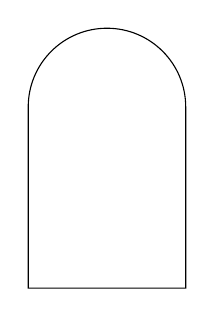
\begin{tikzpicture}
        \draw (0,0) -- (2,0) -- (2,2.3) arc (0:180:1) -- cycle;
    \end{tikzpicture}
\end{center}
\item (002831)已知函数$f(x)=\sqrt{ax^2+x+1}$.\\
(1) 若函数$y=f(x)$的定义域为$(-\infty ,+\infty)$, 求实数$a$的取值范围;\\
(2) 若函数$y=f(x)$的值域为$[0,+\infty)$, 求实数$a$的取值范围.
\item (002832)已知函数$f(x)=\sqrt x$, 函数$g(x)=\sqrt{1-x}-\sqrt x$, 则函数$y=f(x)+g(x)$的定义域为\blank{50}.
\item (002833)已知函数$y=f(x)$的定义域为$[1,4]$, 则函数$y=\dfrac{f(2x)}{x-2}$的定义域是\blank{50}.
\item (002834)(1)设函数$D(x)=\begin{cases} 1, & x\in \mathbf{Q}, \\  0, &x\notin\mathbf{Q}. \end{cases}$ 令$F(x)=D(\sqrt 2x)$, 则$F(1)=$\blank{50};\\
(2) 已知函数$f(x)=\begin{cases} 2-x, & x<-2, \\ x^2, & -2\le x<1, \\ x, & x\ge 1. \end{cases}$ 若$f(x)=2$, 则$x$=\blank{50}.
\item (002835)已知$f(x)=\begin{cases} x-2, & x>8, \\ f(x+3), & x\le 8, \end{cases}$ 则$f(2)=$\blank{50}.
\item (002836)设常数$a\in \mathbf{R}$, $f(x)=\begin{cases}x+a, &x<a, \\ \dfrac 1x+a, & x\ge a. \end{cases}$ 若$f(2)=2$, 则$a=$\blank{50}.
\item (002837)已知函数$f(x)=\begin{cases} \sqrt x, & x>1, \\ x, &x\le 1,  \end{cases}$ 函数$g(x)=1-\sqrt x$. 求函数$y=f(x)+g(x)$的解析式及定义域.
\item (002838)*设$D$是含数$1$的有限实数集, $f(x)$是定义在$D$上的函数, 若$f(x)$的图像绕原点逆时针旋转$\dfrac \pi6$后与原图像重合, 则在以下各项中, $f(1)$的可能取值只能是\bracket{20}
\fourch{$\sqrt3$}{$\dfrac{\sqrt{3}}2$}{$\dfrac{\sqrt{3}}3$}{$0$}
\item (002839)设常数$p\in \mathbf{R}$, 设函数$f(x)=\log_2\dfrac{x+1}{x-1}+\log_2(x-1)+\log_2(p-x)$.\\
(1) 求$p$的取值范围以及函数$y=f(x)$的定义域;\\
(2) 若$y=f(x)$存在最大值, 求$p$的取值范围, 并求出最大值.
\item (002840)已知$xy<0$, 且$4x^2-9y^2=36$. 问: 能否由此条件将$y$表示成$x$的函数? 若能, 求出该函数的解析式; 若不能, 说明理由.
\item (002841)已知常数$a\in \mathbf{R}$, 函数$g(x)=\dfrac x{x+2}$, 函数$h(x)=\dfrac 1{x+a}$. 设函数$F(x)=g(x)\cdot h(x)$, $D_F$是其定义域; $f(x)=g(x)-h(x)$, $D_f$是其定义域.\\
(1) 设$a=2$, 求函数$F(x)$的值域;\\
(2) 对于给定的常数$a$, 是否存在实数$t$, 使得$f(t)=0$成立? 若存在, 求出这样的所有$t$的值; 若不存在, 说明理由;\\
(3) *是否存在常数$a$的值, 使得对于任意$x\in {D_f}\cap \mathbf{R}^+$, 有$f(x)\ge 0$恒成立? 若存在, 求出所有这样的a的值; 若不存在, 说明理由.
\item (002842)给定六个函数: \textcircled{1} $y=\dfrac 1x$; \textcircled{2} $y=x^2+1$; \textcircled{3} $y={x^{-\frac 13}}$; \textcircled{4} $y=2^x$; \textcircled{5} $y=\log_2x$; \textcircled{6} $y=\sqrt{x^2-1}+\sqrt{1-x^2}$.\\
在这六个函数中, 是奇函数但不是偶函数的是\blank{50}, 是偶函数但不是奇函数的是\blank{50}, 既不是奇函数也不是偶函数的是\blank{50}, 既是奇函数又是偶函数的是\blank{50}.
\item (002843)设常数$a$、$b\in \mathbf{R}$. 若定义在$[a-2,2a]$上的$f(x)=ax^2+bx$是偶函数, 则$a=$\blank{50}, $b=$\blank{50}.
\item (002844)设常数$a$、$b\in \mathbf{R}$. 若定义在$[a-1,a+1]$上的$f(x)=ax^2+x+b$是奇函数, 则$a=$\blank{50}, $b=$\blank{50}.
\item (002845)若函数$f(x)=\dfrac{(x+1)(x+a)}x$为奇函数, 则实数$f(x)$\blank{50}.
\item (002846)设函数$y=f(x)$为定义在$\mathbf{R}$上的函数, 则命题: ``$f(-1)\ne f(1)$且$f(-1)\ne -f(1)$''是命题``$y=f(x)$既不是奇函数也不是偶函数''的\blank{50}条件(填``充分不必要''、``必要不充分''、``充要''、``既不充分也不必要''之中一个).
\item (002847)设$y=f(x)$是定义在$\mathbf{R}$上的函数, 当$x\ge 0$时, $f(x)=x^2-2x$.\\
(1) 当$y=f(x)$为奇函数时, 则当$x<0$时, $f(x)$=\blank{50};\\
(2) 当$y=f(x)$为偶函数时, 则当$x<0$时, $f(x)$=\blank{50}.
\item (002848)设奇函数$y=f(x)$的定义域为$[-5, 5]$.若当$x\in [0,5]$时, $y=f(x)$的图像如图, 则不等式$xf(x)<0$的解是\blank{50}.
\begin{center}
    \begin{tikzpicture}[>=stealth]
        \draw [->] (-1,0) -- (6,0) node [below] {$x$};
        \draw [->] (0,-2.5) -- (0,2.5) node [left] {$y$};
        \draw (2,0) node [below] {$2$};
        \draw (5,0) node [above] {$5$};
        \draw [domain = 0:2,samples = 100] plot (\x,-\x*\x+2*\x);
        \draw [domain = 2:5,samples = 100] plot (\x, \x*\x/2-4*\x+6);
        \draw [dashed] (5,0) -- (5,-1.5);
        \draw (0,0) node [below left] {$O$};
    \end{tikzpicture}
\end{center}
\item (002849)若定义在$\mathbf{R}$上的两个函数$y=f(x)$、$y=g(x)$均为奇函数. 设$F(x)=af(x)+bg(x)+1$.\\
(1) 若$F(-2)=10$, 则$F(2)=$\blank{50};\\
(2) 若函数$y=F(x)$在$(0,+\infty)$上存在最大值$4$, 则$y=F(x)$在$(-\infty ,0)$上的最小值为\blank{50}.
\item (002850)判断下列函数$y=f(x)$的奇偶性:\\
(1) $f(x)=(x-1)\cdot \sqrt{\dfrac{1+x}{1-x}}$;\\
(2)$f(x)=\begin{cases} x(1-x), & x<0, \\ x(1+x),& x>0. \end{cases}$.
\item (002851)已知函数$f(x)=x^2-2a|x-1|$, $x\in \mathbf{R}$, 常数$a\in \mathbf{R}$.\\
(1) 求证: 函数$y=f(x)$不是奇函数;\\
(2) 若函数$y=f(x)$是偶函数, 求实数$f(x)=\log_3| 2x+a |$的值.
\item (002852)判断下列函数$y=f(x)$的奇偶性:\\
(1) $f(x)=\dfrac 1{a^x-1}+\dfrac 12$(常数$a>0$且$a\ne 1$);\\
(2) $f(x)=\dfrac{ax}{x^2-a}$(常数$a\in \mathbf{R}$).
\item (002853)设$y=f(x)$是定义在$\mathbf{R}$上的函数, 则下列叙述正确的是\bracket{20} .
\twoch{$y=f(x)f(-x)$是奇函数}{$y=f(x)|f(-x)|$是奇函数}{$y=f(x)-f(-x)$是偶函数	}{$y=f(x)+f(-x)$是偶函数}
\item (002854)设函数$y=f(x)$为定义在$\mathbf{R}$上的函数, 则``$f(0)\ne 0$''是``函数$y=f(x)$不是奇函数''的\bracket{20}.
\twoch{充分非必要条件}{必要非充分条件}{充要条件}{既不是充分条件, 也不是必要条件}
\item (002855)设$y=f(x)$是定义在$\mathbf{R}$上的奇函数, 当$x<0$时, $f(x)=\lg(2-x)$, 则$x\in \mathbf{R}$时, $f(x)$=\blank{50}.
\item (002856)判断下列函数$y=f(x)$的奇偶性, 并说明理由:\\
(1) $f(x)=x^3-\dfrac 1x$;\\
(2) $f(x)=\dfrac{|x+3|-3}{\sqrt{4-x^2}}$.
\item (002857)根据常数$a$的不同取值, 讨论下列函数$y=f(x)$的奇偶性, 并说明理由:\\
(1) $f(a)\ge f(0)$;\\
(2) $f(x)=x|x-a|$.
\item (002858)设函数$y=f(x)$是定义在$\mathbf{R}$上的奇函数. 若$x>0$时, $f(x)=\lg x$.\\
(1) 求方程$f(x)=0$的解集;\\
(2) 求不等式$f(x)>-1$的解集.
\item (002859)是否存在实数$b$, 使得函数$g(x)=\dfrac{2^x}{{4^x}-b}$是奇函数? 若存在, 求$b$的值; 若不存在, 说明理由.
\item (002860)常数$a\in \mathbf{R}$. 若函数$f(x)=\lg(10^x+1)+ax$是偶函数, 则$a=$\blank{50}.
\item (002861)已知$y=f(x)$为定义在$\mathbf{R}$上的奇函数, $y=g(x)$为定义在$\mathbf{R}$上的偶函数, 且任意$x\in \mathbf{R}$, 都有$f(x)=g(x)+\dfrac{1}{x^2+x+1}$, 则$f(1)+g(1)=$\blank{50}.
\item (002862)设常数$a\ne 0$. 若函数$f(x)=\lg \dfrac{x+1-2a}{x+1+3a}$. 是否存在实数$a$, 使函数$y=f(x)$为奇函数或偶函数? 若存在, 求出$a$的值, 并判断相应的$y=f(x)$的奇偶性; 若不存在, 说明理由.
\item (002863)函数$y=\dfrac 1{x^2-4x+5}$的图像关于\bracket{20}.
\fourch{$y$轴对称}{原点对称}{直线$x=2$对称}{点$(2,1)$对称}
\item (002864)函数$y=x+\dfrac 1{x-1}$的图像关于\bracket{20}.
\fourch{点$(1,1)$对称}{点$(-1,1)$对称}{点$(1,-1)$对称}{点$(-1,-1)$对称}
\item (002865)若函数$y=f(x)$的定义域为$\mathbf{R}$, 且$f(x-1)=-f(3-x)$, 则$y=f(x)$的图像关于\bracket{20}.
\fourch{原点中心对称}{点$(1,0)$中心对称}{点$(2,0)$中心对称}{点$(4,0)$中心对称}
\item (002866)设常数$a,b\in \mathbf{R}$.若函数$y=x^2+ax$在区间$[a,b]$上的图像关于直线$x=1$对称, 则$b=$\blank{50}.
\item (002867)已知函数$y=f(x)$满足: 对于任意$x\in \mathbf{R}$, 都有$f(x+1)=-f(x)$. 若$f(1)=1$, 则$f(4)=$\blank{50}; $f(2015)=$\blank{50}.
\item (002868)已知函数$y=f(x)$图像关于$(1,0)$对称. 若$x\le 1$时, $f(x)=x^2-1$, 则$f(x)=$\blank{50}.
\item (002869)已知函数$y=f(x)$满足: 对于任意$x\in \mathbf{R}$, 都有$f(x+3)=f(x)$. 若$x\in [0,3)$时, $f(x)=x-1$, 则$x\in [6,9)$时, $f(x)=$\blank{50}.
\item (002870)设常数$a\in \mathbf{R}$.已知函数$y=f(x)$满足: 对于任意$x\in \mathbf{R}$, 都有$f(x-1)=f(1-x)$. 若函数$y=f(x)$图像总是关于直线$x=a$对称, 则$a$=\blank{50}.
\item (002871)设常数$a\in \mathbf{R}$.若直线$x=2$是函数$f(x)=\log_3|2x+a|$的图像的一条对称轴, 则$a$=\blank{50}.
\item (002872)设函数$y=f(x)$为$\mathbf{R}$上的奇函数, 且对于任意$x\in \mathbf{R}$都有$f(x+2)=-f(x)$.\\
(1) 求证: 函数$y=f(x)$为周期函数;\\
(2) 对于任意$x\in \mathbf{R}$, 求证: $f(1+x)=f(1-x)$;\\
(3) 设$0\le x\le 1$时, $f(x)=\dfrac 12x$. 求函数$y=f(x)+\dfrac 12$在$-4\le x\le 4$时的所有零点;\\
(4) 设$-1\le x\le 1$时, $f(x)=\sin x$.\\
\textcircled{1} 写出$1\le x\le 5$时, $y=f(x)$的解析式;\\
\textcircled{2} 求$y=f(x)$在$\mathbf{R}$上的解析式.
\item (002873)常数$a$、$b\in \mathbf{R}$. 函数$f(x)=\dfrac x{\sqrt 3}+\dfrac 1{x+a}+b$的图像关于点$(1,2)$对称.\\
(1) 求$y=f(x)$的解析式;\\
(2) *若$y=f(x)$的图像关于某一条直线对称, 写出这样的一条对称轴直线的方程(无需证明).
\item (002874)函数$y=\log_2\dfrac{2-x}{2+x}$的图像关于\bracket{20}.
\fourch{原点对称}{$y$轴对称}{直线$y=x$对称}{直线$y=-x$对称}
\item (002875)函数$y=\log_2(2-2^x)$的图像关于\bracket{20}.
\fourch{原点对称}{$y$轴对称}{直线$y=x$对称}{直线$y=-x$对称}
\item (002876)设常数$a$、$b\in \mathbf{R}$. 若二次函数$f(x)=ax^2+bx+1$满足: 对任意$t\in \mathbf{R}$, $f(2+t)=f(2-t)$, 则$\dfrac ba=$\blank{50}.
\item (002877)设定义在$\mathbf{R}$上的函数$y=f(x)$的图像关于直线$x=1$对称. 若$x\ge 1$时, $f(x)=1-3^{x-1}$, 则$x<1$时, $f(x)=$\blank{50}.
\item (002878)设函数$y=\log_2(x+3)$的图像与函数$y=f(x)$的图像关于直线$x=1$对称. \textcircled{1} $f(1)$=\blank{50}; \textcircled{2} 若$f(a)$有意义, 则$f(a)=$\blank{50}(结果用$a$的表达式表示).
\item (002879)已知定义域为$\mathbf{R}$的函数$y=f(x)$是偶函数, 并且其图像关于直线$x=1$对称.\\
(1) 若$f(0)=1$, $f(1)=2$, 求$f(15)+2f(20)$的值;\\
(2) 设$x\in [0,1]$时, $f(x)=x^3$.\\
\textcircled{1} $1<x\le 2$时, 求$y=f(x)$的解析式;\\
\textcircled{2} $-2\le x<0$时, 求$y=f(x)$的解析式;\\
\textcircled{3} 求函数$y=f(x)-\dfrac 18$在$[-2,2]$上的所有零点;\\
\textcircled{4} 求$y=f(x)$在$\mathbf{R}$上的解析式.
\item (002880)已知$f(x)$是定义域为$(-\infty,+\infty)$的奇函数, 满足$f(1-x)=f(1+x)$. 若$f(1)=2$, 则$f(1)+f(2)+f(3)+\cdots +f(50)=$\bracket{20}.
\fourch{$-50$}{$0$}{$2$}{$50$}
\item (002881)已知函数$y=f(x)$对一切$u,v\in \mathbf{R}$, 都有$f(u+v)=f(u)+f(v)$.\\
(1)	求证: $y=f(x)$是奇函数;\\ 
(2) 若$f(-3)=a$, 用$a$表示$f(6)$以及$f(300)$.
\item (002882)已知定义在$\mathbf{R}$上的函数$y=f(x)$是奇函数, 且$y=f(x)$也是以4为周期的一个周期函数.\\
(1) 若$f(1)=1$, 则$f(-1)+f(0)=$\blank{50}; $f(10)+f(11)=$\blank{50};\\
(2) *若$f(1)=0$, 则在区间$[-3,3]$上的零点的个数的最小值为\blank{50}.
\item (002883)*设定义在$\mathbf{R}$上的函数$y=f(x)$的满足: 对于任意$x\in \mathbf{R}$, 恒有$f(-x+1)=-f(x+1)$且$f(-x-1)=-f(x-1)$. 则下面命题中, 正确的命题的序号是\blank{50}.\\
\textcircled{1} 函数$y=f(x)$是偶函数; \textcircled{2} $2$是$y=f(x)$的周期; \textcircled{3} 函数$y=f(x)$图像关于$(1,0)$对称; \textcircled{4} 函数$y=f(x)$图像关于$(3,0)$对称.
\item (002884)下列函数中, 在其定义域上是单调函数的序号为\blank{50}.\\
\textcircled{1} $y=\dfrac{2-x}x$; \textcircled{2} $y=x-\dfrac 1x$; \textcircled{3} $y={3^{x-1}}$; \textcircled{4} $y=ln\dfrac 1x$; \textcircled{5} $y=tanx$.
\item (002885)函数$y=|x-1|$递减区间的是\blank{50}.
\item (002886)函数$y=x+\dfrac 2x$($x>0$)的递减区间是\blank{50}.
\item (002887)函数$y=(\dfrac 12)^{x^2}$的递减区间是\blank{50}.
\item (002888)函数$y=\dfrac 1{\sqrt{x^2+2x-3}}$的递增区间是\blank{50}.
\item (002889)设常数$a\in \mathbf{R}$.若$y=\dfrac{ax}{x+1}$在区间$(-1,+\infty)$上递增, 则$a$的取值范围是\blank{50}.
\item (002890)设常数$a\in \mathbf{R}$.若函数$y=x^2+ax+1$在$(-\infty,2]$上递减, 则$a$的取值范围是\blank{50}.
\item (002891)若函数$y=f(x)$, $y=g(x)$均为$\mathbf{R}$上增函数, 则下列命题中, 正确的命题的序号是\blank{50}.\\
\textcircled{1} $y=f(x)+g(x)$为增函数; \textcircled{2} $y=f(x)\cdot g(x)$为增函数; \textcircled{3} $y=f(g(x))$为增函数.
\item (002892)若$y=f(x)$为$\mathbf{R}$上的奇函数, 且在$(-\infty,0)$上是减函数, 又$f(-2)=0$, 则$f(x)\le 0$的解集为\blank{50}.
\item (002893)设常数$a\in \mathbf{R}$. 若函数$f(x)=\begin{cases} x+a,& x<1, \\ x^2,& x\ge 1 \end{cases}$在$\mathbf{R}$上递增, 则$a$的取值范围为\blank{50}.
\item (002894)设函数$f(x)=\mathrm{e}^x+\dfrac 1{\mathrm{e}^x}$.\\
(1) 求证: $y=f(x)$在$\mathbf{R}$上不是增函数;\\
(2) 求证: $y=f(x)$在$[0,+\infty)$上是增函数.
\item (002895)设常数$a\in \mathbf{R}$. 若$y=\log_{\frac 12}(x^2-ax+2)$在$[-1,+\infty)$上是减函数, 求$a$的取值范围.
\item (002896)已知定义在区间$(-1,1)$上的函数$y=f(x)$是奇函数, 也是减函数. 若$f(1-a)+f(1-a^2)<0$, 求实数$a$的取值范围.
\item (002897)下列函数中, 在区间$(0 ,+\infty)$上递增的函数的序号为\blank{50}.\\
\textcircled{1} $y=|x+1|$;  \textcircled{2} $y=x-\dfrac 1x$;    \textcircled{3} $y={x^{\frac 12}}$;    \textcircled{4} $y=\sqrt{1-\dfrac 1x}$; \textcircled{5} $y=\lg x$.
\item (002898)函数$y=\log_{0.7}(x^2-3x+2)$的单调减区间为\blank{50}.
\item (002899)已知$y=f(x)$是偶函数, 且在区间$[0,4]$上递减. 记$a=f(2)$, $b=f(-3)$, $c=f(-4)$, 则将$a,b,c$按从小到大的顺序排列是	\blank{50}.
\item (002900)设常数$a\in \mathbf{R}$. ``$a=1$''是``$f(x)=|x-a|$在区间$[1, +\infty)$上为增函数''的\blank{50}条件(填: ``充分不必要''、``必要不充分''、``充要''、``既不充分也不必要''之一).
\item (002901)(1) 设常数$a\in \mathbf{R}$.若函数$y=\dfrac 1{x-a}$在区间$(0,+\infty)$上单调, 则$a$的取值范围为\blank{50}.\\
(2) 设常数$k\in \mathbf{R}$.若函数$f(x)=kx^2-4x+8$在区间$[5,20]$上单调递减, 则$k$的取值范围是\blank{50}.
\item (002902)*设$f(x)$、$g(x)$、$h(x)$是定义域为$R$的三个函数, 对于下列命题:\\
\textcircled{1} 若$f(x)+g(x)$、$f(x)+h(x)$、$g(x)+h(x)$均为增函数, 则$f(x)$、$g(x)$、$h(x)$中至少有一个是增函数;\\
\textcircled{2} 若$f(x)+g(x)$、$f(x)+h(x)$、$g(x)+h(x)$均是以$T$为周期的函数, 则$f(x)$、$g(x)$、$h(x)$均是以$T$为周期的函数, 下列判断正确的是\bracket{20}.
\twoch{\textcircled{1}和\textcircled{2}均为真命题}{\textcircled{1}和\textcircled{2}均为假命题}{\textcircled{1}为真命题, \textcircled{2}为假命题}{\textcircled{1}为假命题, \textcircled{2}为真命题}
\item (002903)设常数$a,b\in \mathbf{R}$. 已知$f(x)=\dfrac{ax^2+1}{x+b}$是奇函数, $f(1)=5$.\\
(1) 求$a,b$的值;\\
(2) 求证: $y=f(x)$在区间$(0,\dfrac 12]$上是减函数.
\item (002904)求证: 函数$f(x)=\dfrac 1x-\lg\dfrac{1+x}{1-x}$是奇函数, 且在区间$(0,1)$上递减.
\item (002905)设常数$a\in \mathbf{R}$.若函数$f(x)=\log_a(2-ax)$在$[0,1]$上是减函数, 求$a$的取值范围.
\item (002906)已知定义$\mathbf{R}$上的函数$y=f(x)$满足下面两个条件:\\
(I) 对于任意$x_1,x_2\in \mathbf{R}$, 都有$f(x_1+x_2)=f(x_1)+f(x_2)$; (II)当$x>0$时, $f(x)>0$, 且$f(1)=1$.\\
(1) 求证: $y=f(x)$是奇函数;\\
(2) 求证: $y=f(x)$在$\mathbf{R}$上是增函数;\\
(3) *解不等式$f(x^2-1)<2$.
\item (002907)函数$y=x^{-\frac 32}$的定义域为\blank{50}.
\item (002908)下列命题中, 正确的命题的序号是\blank{50}.\\
\textcircled{1} 当$\alpha =0$时, 函数$y={x^{\alpha }}$的图像是一条直线;\\
\textcircled{2} 幂函数的图像都经过(0, 0)和(1, 1)点;\\
\textcircled{3} 当$\alpha <0$且$y={x^{\alpha }}$是奇函数时, 它也是减函数;\\
\textcircled{4} 第四象限不可能有幂函数的图像.
\item (002909)图中曲线是幂函数$y=x^n$在第一象限的图像, 已知$n$取$\pm 2$, $\pm\dfrac 12$四个值, 则相应于曲线$c_1,c_2,c_3,c_4$的$n$依次为\bracket{20}.
\begin{center}
    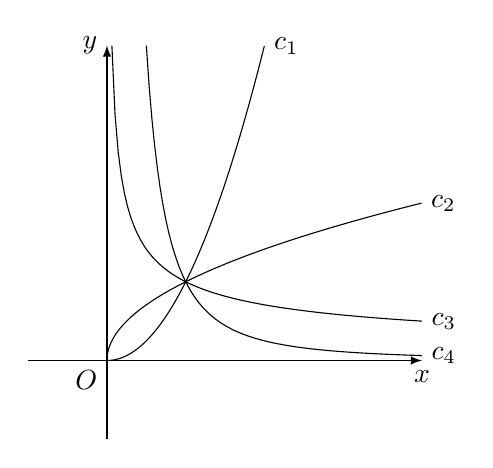
\begin{tikzpicture}[>=latex]
        \draw [->] (-1,0) -- (4,0) node [below] {$x$};
        \draw [->] (0,-1) -- (0,4) node [left] {$y$};
        \draw (0,0) node [below left] {$O$};
        \draw [domain = 0:2, samples = 100] plot (\x,\x*\x) node [right] {$c_1$};
        \draw [domain = 0:2, samples = 100] plot (\x*\x,\x) node [right] {$c_2$};
        \draw [domain = 0.0625:4, samples = 100] plot (\x, {1/sqrt(\x)}) node [right] {$c_3$};
        \draw [domain = 0.5:4, samples = 100] plot (\x, {1/\x/\x}) node [right] {$c_4$};
    \end{tikzpicture}
    \end{center}
\fourch{$-2,-\dfrac 12,\dfrac 12,2$}{$2,\dfrac 12,-\dfrac 12,-2$
}{$-\dfrac 12,-2,2,\dfrac 12$}{$2,\dfrac 12,-2,-\dfrac 12$}
\item (002910)下列函数的图像为(A)、(B)、(C)、(D)之一, 试将正确的字母标号填在相应函数后面的横线上.
\begin{center}
    \begin{tikzpicture}[>=latex,scale = 0.5]
        \draw [->] (-3,0) -- (3,0) node [below] {$x$};
        \draw [->] (0,-3) -- (0,3) node [left] {$y$};
        \draw (0,0) node [below right] {$O$};
        \draw [domain = {-3^(1/4)}:{3^(1/4)}] plot (\x*\x*\x,\x*\x*\x*\x);
        \draw (0,-3) node [below] {(A)};
    \end{tikzpicture}
    \begin{tikzpicture}[>=latex,scale = 0.5]
        \draw [->] (-3,0) -- (3,0) node [below] {$x$};
        \draw [->] (0,-3) -- (0,3) node [left] {$y$};
        \draw (0,0) node [below right] {$O$};
        \draw [domain = {-3^(1/5)}:{3^(1/5)}] plot (\x*\x*\x,\x*\x*\x*\x*\x);
        \draw (0,-3) node [below] {(B)};
    \end{tikzpicture}
    \begin{tikzpicture}[>=latex,scale =0.5]
        \draw [->] (-3,0) -- (3,0) node [below] {$x$};
        \draw [->] (0,-3) -- (0,3) node [left] {$y$};
        \draw (0,0) node [below right] {$O$};
        \draw [domain = {0}:{3^(1/3)}] plot (\x*\x,\x*\x*\x);
        \draw (0,-3) node [below] {(C)};
    \end{tikzpicture}
    \begin{tikzpicture}[>=latex,scale = 0.5]
        \draw [->] (-3,0) -- (3,0) node [below] {$x$};
        \draw [->] (0,-3) -- (0,3) node [left] {$y$};
        \draw (0,0) node [below right] {$O$};
        \draw [domain = {3^(-3/2)}:3] plot (\x,{\x^(-2/3)}) plot (-\x,{\x^(-2/3)});
        \draw (0,-3) node [below] {(D)};
    \end{tikzpicture}
    \end{center}
(1) $y=x^\frac 32$\blank{50}; (2) $y=x^\frac 43$\blank{50}; (3) $y=x^\frac 53$\blank{50}; (4) $y=x^{-\frac 23}$\blank{50}.
\item (002911)已知$\alpha\in \{-2,-1,-\dfrac 12,\dfrac 12,1,2,3\}$, 若幂函数$f(x)=x^\alpha$为奇函数, 且在$(0,+\infty)$上递减, 则$\alpha=$\blank{50}.
\item (002912)函数$y=f(x)$满足两个条件:
\textcircled{1} $y=f(x)$是两个幂函数的和函数; \textcircled{2} $y=f(x)$的最小值为2, 则$y=f(x)$的解析式可以是\blank{50}.
\item (002913)若集合$A=\{y|y={x^{\frac 13}}, \ -1\le x\le 1\}$, $B=\{y|y={x^{-\frac 12}}\}$, 则$A\cap B$等于\bracket{20}.
\fourch{$(0,1]$}{$[-1,1]$}{$\{1\}$}{$\{0,1\}$}
\item (002914)设常数$m\in \mathbf{R}$. 若幂函数$y=(m^2-m-1)x^{m^2-2m-1}$在$(0,+\infty)$上是增函数, 则$m$的值为\blank{50}.
\item (002915)设常数$n\in \mathbf{Z}$. 若函数$y=x^{n^2-2n-3}$的图像与两条坐标轴都无公共点, 且图像关于$y$轴对称, 则$n$的值为\blank{50}.
\item (002916)函数$y=1-(x+2)^{-2}$可以先将幂函数$y=x^{-2}$的图像向\blank{50}平移$2$个单位, 再以\blank{50}轴为对称轴作对称变换, 最后向\blank{50}平移$1$个单位.
\item (002917)在$f(x)=(2m^2-7m-9)x^{m^2-9m+19}$中, 当实数$m$为何值时,\\
(1) $y=f(x)$是正比例函数, 且它的图像的倾斜角为钝角?\\
(2) $y=f(x)$是反比例函数, 且它的图像在第一, 三象限?
\item (002918)设常数$t\in \mathbf{Z}$. 已知幂函数$y=(t^3-t+1){x^{\frac 13(1+2t-t^2)}}$是偶函数, 且在区间$(0,+\infty)$上是增函数, 求整数$t$的值, 并作出相应的幂函数的大致图像.
\item (002919)设$a\in \mathbf{R}$.\\
(1) 若$(a+2)^{\frac 23}>{(1-2a)}^{\frac 23}$, 求$a$的取值范围;\\
(2) 若$(a+2)^{-\frac 13}>(1-2a)^{-\frac 13}$, 求$a$的取值范围.
\item (002920)已知函数: \textcircled{1} $y=\dfrac 1x$; \textcircled{2} $y=x^{\dfrac 12}$; \textcircled{3} $y=x^{-\dfrac 12}$; \textcircled{4} $y={x^{\dfrac 23}}$; \textcircled{5} $y=x^{-\dfrac 23}$, 填写分别具有下列性质的函数序号:\\ 
(1) 图像与$x$轴有公共点的:\blank{50};\\
(2) 图像关于原点对称的:\blank{50};\\
(3) 定义域内递减的:\blank{50};\\
(4) 在定义域内有反函数的:\blank{50}.
\item (002921)函数$y=-(x+1)^{-3}$的图像可以先将幂函数$y=x^{-3}$的图像向\blank{50}平移1个单位, 再以\blank{50}轴为对称轴作对称变换.
\item (002922)设$\alpha \in \{-3,-\dfrac 23,-\dfrac 12,-\dfrac 13,\dfrac 13,1,\dfrac 32,2\}$. 已知幂函数$y=x^{\alpha}$是奇函数, 且在区间$(0,+\infty)$上是减函数, 则满足条件的$\alpha$的值是\blank{50}.
\item (002923)下列关于幂函数图像及性质的叙述中, 正确的叙述的序号是\blank{50}.\\
\textcircled{1} 对于一个确定的幂函数, 第二、三象限不可能同时有该幂函数的图像上的点;\\
\textcircled{2} 若某个幂函数图像过$(-1,-1)$, 则该幂函数是奇函数;\\
\textcircled{3} 若某个幂函数在定义域上递增, 则该幂函数图像必经过原点;\\
\textcircled{4} 幂函数图像不会经过点$(-\dfrac 12,8)$以及$(-8,-4)$.
\item (002924)设$y=f(x)$与$y=g(x)$是两个不同的幂函数, 集合$M=\{x|f(x)=g(x)  \}$, 则集合$M$中的元素是\bracket{20}.
\fourch{$1$或$2$}{$1$或$3$}{$1$或$2$或$3$}{$1$或$2$或$3$或$4$}
\item (002925)已知幂函数$y=x^{\frac qp}$($p\in \mathbf{N}^*,\ q\in \mathbf{N}^*$, $p,q$互质)的图像如图所示, 则\bracket{20}.
\begin{center}
    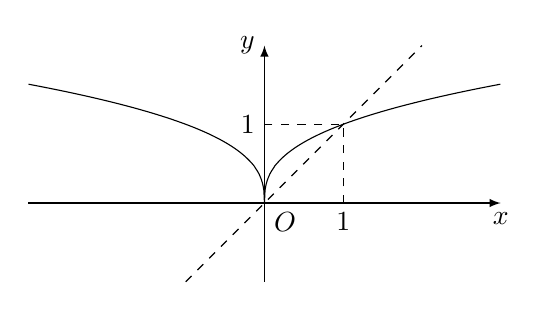
\begin{tikzpicture}[>=latex]
        \draw [->] (-3,0) -- (3,0) node [below] {$x$};
        \draw [->] (0,-1) -- (0,2) node [left] {$y$};
        \draw (0,0) node [below right] {$O$};
        \draw [dashed] (-1,-1) -- (2,2);
        \draw [domain = 0:3, samples = 400] plot (\x,{\x^(3/8)}) plot (-\x,{\x^(3/8)});
        \draw [dashed] (1,0) node [below] {$1$} -- (1,1) -- (0,1) node [left] {$1$};
    \end{tikzpicture}
\end{center}
\twoch{$p,q$均为奇数}{$p$是奇数, $q$是偶数, 且$0<\dfrac qp<1$}{$p$是偶数, $q$是奇数}{$p$是奇数, $q$是偶数, 且$\dfrac qp>1$}
\item (002926)若$(x+1)^{-\frac 13}<(3-2x)^{-\frac 13}$, 求实数$x$的取值范围.
\item (002927)设常数$a,b$满足$a>b>0$. 已知函数$f(x)=\dfrac{x+a}{x+b}$.
(1) 写出函数$y=f(x)$的单调性;\\
(2) 写出函数$y=f(x)$图像的一个对称中心的坐标.
\item (002928)已知函数$f(x)=\dfrac{x^{\frac 13}-x^{-\frac 13}}5$, $g(x)=\dfrac{x^{\frac 13}+x^{-\frac 13}}5$.\\
(1) 分别计算$f(4)-5f(2)g(2)$和$f(9)-5f(3)g(3)$的值;\\
(2) 由(1)概括出涉及函数$y=f(x)$和$y=g(x)$的, 对所有不等于零的实数$x$都成立的一个等式, 并加以证明.
\item (002929)*设常数$a,b$满足$a>b>0$. 已知函数$f(x)=\dfrac{x+a}{x+b}$. 证明: 该函数图像的对称中心是唯一的.
\item (002930)函数$y=\log_2 \dfrac 1{x-1}$的反函数是\blank{50}.
\item (002931)函数$y=x^2$($x\le 0$)的反函数是\blank{50}.
\item (002932)函数$y=\dfrac{2^x}{{2^x}-1}$($x>0$)的反函数是\blank{50}.
\item (002933)已知函数$y=f(x)$的反函数是$f^{-1}(x)=\dfrac{4x+3}{2x-1}$, 则$f(x)$=\blank{50}.
\item (002934)记$y=f^{-1}(x)$是$y=f(x)$的反函数. 若函数$f(x)=\log_3x$, 则$f^{-1}(-\log_9 2)$=\blank{50}.
\item (002935)若命题``函数$y=x+\dfrac ax$在区间$[1,2]$上存在反函数''为真命题, 则在下列值中, 能作为实数$a$的值的序号是\blank{50}.\\
\textcircled{1} $a=-1$; \textcircled{2} $a=1$; \textcircled{3} $a=\sqrt 2$; \textcircled{4} $a=\sqrt 5$.
\item (002936)若函数$f(x)=1-\sqrt{1-x^2}\ (-1\le x\le 0)$,
请画出函数$y={f^{-1}}(x)$的大致图像.
\begin{center}
    \begin{tikzpicture}[>=latex,scale =1.8]
        \foreach \i in {-1,-0.5,0,0.5,1} {\draw [dashed, gray!90] (\i,-1) -- (\i,1) (-1,\i) -- (1,\i);};
        \draw [->] (-1.5,0) -- (1.5,0) node [below] {$x$};
        \draw [->] (0,-1.5) -- (0,1.5) node [left] {$y$};
        \draw (0,0) node [below left] {$O$};
        \draw (1,0) node [below] {$1$} (0,1) node [left] {$1$};
    \end{tikzpicture}
\end{center}
\item (002937)已知定义在$\mathbf{R}$上的函数$y=f(x)$是奇函数, 且有反函数$y=f^{-1}(x)$. 若$a,b$是两个实数, 则下列点中, 必在$y=f^{-1}(x)$的图像上的点的序号是\blank{50}.\\
\textcircled{1} $(-f(a),a)$; \textcircled{2} $(-f(a),-a)$;\textcircled{3} $(-b,-f(b))$; \textcircled{4} $(b,-f^{-1}(-b))$.
\item (002938)已知定义在$\mathbf{R}$上的函数$y=f(x)$的反函数为$y=f^{-1}(x)$.若$y=f(x+1)$的图像过点$(-\dfrac 12,1)$, 则$y=f^{-1}(x+1)$的图像必过\bracket{20}.
\fourch{$(1,-\dfrac 12)$}{$(1,\dfrac 12)$}{$(0,-\dfrac 12)$}{$(0,\dfrac 12)$}
\item (002939)设常数$a\ne 0$. 若函数$f(x)=\dfrac{1-ax}{1+ax}$的图像关于直线$y=x$对称, 求实数$a$的值以及$y=f(x)$的反函数$y=f^{-1}(x)$.
\item (002940)记$y=f^{-1}(x)$是$y=f(x)$的反函数.\\
(1) 若函数$f(x+1)=\dfrac x{x+1}$, 求函数$y=f^{-1}(x+1)$的解析式;\\
(2) 设函数$f(x)=\dfrac{1-2x}{1+x}$. 若$y=g(x)$的图像与$y=f^{-1}(x+1)$的图像关于直线$y=x$对称, 求$y=g(x)$的解析式.
\item (002941)(1) 函数$y=x^2+2x-3\ (x\ge 0)$的反函数为\blank{50};\\
(2) 函数$y=\dfrac{\mathrm{e}^x-1}{{\mathrm{e}}^x+1}$的反函数为\blank{50};\\
(3) 函数$y=x|x|$的反函数为\blank{50}.
\item (002942)已知函数$y=f(x)$是奇函数, 且$y=g(x)$是$y=f(x)$的反函数. 若$x\ge 0$时, $f(x)=3^x-1$, 则$g(-8)$=\blank{50}.
\item (002943)设常数$a\in \mathbf{R}$. 若函数$y=x+\dfrac ax$在区间$[1,2]$上存在反函数, 求$a$的取值范围.
\item (002944)求函数$y=\begin{cases}x^2-2x+2, & x\le 1,\\(\dfrac 12)^x, & x>1  \end{cases}$的反函数.
\item (002945)设常数$a>0$且$a\ne 1$. 求函数$f(x)=\log_a(x+\sqrt{x^2-1})$的反函数.
\item (002946)已知函数$y=f(x)$的图像经过点$(0,-1)$. 若函数$y=f(x+4)$存在反函数$y=g(x)$, 则$y=g(x)$的图像总经过的定点的坐标为\blank{50}.
\item (002947)设$y=f^{-1}(x)$, $y=g^{-1}(x)$分别是定义在$\mathbf{R}$上的函数$y=f(x)$, $y=g(x)$的反函数. 若函数$y=f(x-1)$和$y=g^{-1}(x-3)$的图像关于直线$y=x$对称, 且$g(5)=2018$, 则 $f(4)$的值为\blank{50}.
\item (002948)设$a>0$, 函数$f(x)=\dfrac 1{1+a\cdot 2^x}$.\\
(1) 若$a=1$, 求$f(x)$的反函数$f^{-1}(x)$;\\
(2) 求函数$y=f(x)\cdot f(-x)$的最大值(用$a$表示);\\
(3) *设$g(x)=f(x)-f(x-1)$. 若对任意$x\in (-\infty ,0]$, $g(x)\ge g(0)$恒成立, 求$a$的取值范围.
\item (002949)已知函数$y=f^{-1}(x)$是$y=f(x)$的反函数. 定义: 若对给定的实数$a(a\ne 0)$, 函数$y=f(x+a)$与$y=f^{-1}(x+a)$互为反函数, 则称$y=f(x)$满足``$a$和性质''.\\
(1) 判断函数$g(x)=x^2+1(x>0)$是否满足``$1$和性质'', 并说明理由;\\
(2) *求所有满足``$2$和性质''的一次函数.
\item (002950)若$\log_35=a$, $\log_57=b$ , 用$a,b$表示$\log_{75}63=$\blank{50}.
\item (002951)若$3^a=4^b=6^c$, 且$a,b,c$都是正数, 则$\dfrac{-2ab+2bc+ac}{abc}$的值为\blank{50}.
\item (002952)若不等式$(a-1)^x<1$的解集为$(-\infty,0)$, 则实数$a$的取值范围是\blank{50}.
\item (002953)函数$f(x)=\dfrac{\sqrt{4-x^2}}{\lg |x-1|}$的定义域为\blank{50}.
\item (002954)为了得到函数$y=\lg\dfrac{x+3}{10}$的图像, 只需把函数$y=\lg x$的图像上所有的点\bracket{20}.
\onech{向左平移$3$个单位长度, 再向上平移$1$个单位长度}{向右平移$3$个单位长度, 再向上平移$1$个单位长度}{向左平移$3$个单位长度, 再向下平移$1$个单位长度}{向右平移$3$个单位长度, 再向下平移$1$个单位长度}
\item (002955)设常数$a>0,\ a\ne 1$. 函数$f(x)=a^x$在$[0,1]$上的最大值和最小值之和为$a^2$, 则$a=$\blank{50}.
\item (002956)若集合$A=\{y|y=2\cdot (\dfrac 13)^{|x|}\}$, $B=\{ a|\log_a(3a-1)>0\}$, 则$A\cap B$=\blank{50}.
\item (002957)*已知函数$f(x)=|3^x-1|$, $c<b<a$, 且$f(b)<f(a)<f(c)$, 在下列关系式中, 一定成立的关系式的序号是\blank{50}.
\textcircled{1} $3^a+3^b>2$; \textcircled{2} $3^a+3^b<2$; \textcircled{3} $3^c<1$; \textcircled{4} $3^a+3^c<2$.
\item (002958)已知函数$f(x)=\dfrac{3^x-3^{-x}}{3^x+3^{-x}}$.\\
(1) 证明$f(x)$在$(-\infty,+\infty)$上是增函数;\\
(2) 求$f(x)$的值域.
\item (002959)已知函数$y=(\log_2\dfrac x{2^a})(\log_2\dfrac x4)$, $x\in [\sqrt 2,4]$, 试求该函数的最大值$g(a)$.
\item (002960)已知函数$f(x)=a\cdot 2^x+b\cdot 3^x$, 其中常数$a,b$满足$ab\ne 0$.\\
(1) 若$ab>0$, 判断函数$y=f(x)$的单调性;\\
(2) 若$ab<0$, 求$f(x+1)>f(x)$时$x$的取值范围.
\item (002961)不等式$\log_{\frac 12}(x-1)\ge 1$的解集为\blank{50}.
\item (002962)设常数$a\in \mathbf{R}$. 若函数$f(x)=\dfrac 1{2^x-1}+a$为奇函数, 则$a$=\blank{50}.
\item (002963)若$\log_23=a$, $3^b=7$, 用$a,b$表示$\log_{3\sqrt 7}2$, 则$\log_{3\sqrt 7}2$=\blank{50}.
\item (002964)对于函数$y=f(x)$的定义域中的任意的$x_1,x_2$($x_1\ne x_2$), 有如下结论:\\
\textcircled{1} $f(x_1+x_2)=f(x_1)\cdot f(x_2)$; \textcircled{2} $f(x_1\cdot x_2)=f(x_1)+f(x_2)$;\\ \textcircled{3} $\dfrac{f(x_1)-f(x_2)}x_1-x_2>0$; \textcircled{4} $f(\dfrac{x_1+x_2}2)<\dfrac{f(x_1)+f(x_2)}2$. 
\\当$y=\ln x$时, 上述结论中, 正确结论的序号是\blank{50}.
\item (002965)(1) *函数$y=\log_a|x-b|$在$(0,+\infty)$上递增, 则$a$、$b$满足\bracket{20}.
\fourch{$a>1$且$b\ge 0$}{$a>1$且$b\le 0$}{$0<a<1$且$b\ge 0$}{$0<a<1$且$b\le 0$}
(2) 函数$f(x)=\log_a|ax^2-x| \ (a>0,\ a\ne 1)$在区间$[3,4]$上是增函数, 则实数$a$的范围是\blank{50}.
\item (002966)*已知常数$a>1$, 函数$y=|\log_ax|$的定义域为区间$[m,n]$, 值域为区间$[0,1]$. 若$n-m$的最小值为$\dfrac 56$, 则$a$=\blank{50}.
\item (002967)*设常数$a>0$ ,$a\ne 1$. 已知函数$f(x)=\log_ax$. 若对于任意$x\in [3,+\infty)$都有$|f(x)|\ge 1$成立, 则$a$的取值范围为\blank{50}.
\item (002968)*已知函数$f(x)=2+\log_3 x\ (3\le x\le 27)$.\\
(1) 求函数$y=f(x^2)$的定义域;\\
(2) 求函数$g(x)={[f(x)]}^2+f(x^2)$的值域.
\item (002969)已知定义域为$\mathbf{R}$的函数$y=f(x)$为奇函数, 且满足$f(x+2)=-f(x)$. 当$x\in [0,1]$时, $f(x)=2^x-1$.\\
(1) 求$y=f(x)$在区间$[-1,0)$上的解析式;\\
(2) 求$f(\log_{\frac 12}24)$的值.
\item (002970)*已知函数$f(x)=1+a\cdot (\dfrac 12)^x+(\dfrac 14)^x$.\\
(1) 当$a=1$时, 求函数$y=f(x)$在$(-\infty,0)$上的值域;\\
(2) 对于定义在集合$D$上的函数$y=f(x)$, 如果存在常数$M>0$, 满足: 对任意$x\in D$, 都有$|f(x)|\le M$成立, 则称$f(x)$是$D$上的有界函数, 其中$M$称为函数$f(x)$的一个上界.若函数$y=f(x)$在$[0,+\infty)$上是以$3$为一个上界的有界函数, 求实数$a$的取值范围.
\item (002971)二次函数图像的顶点是$(-1,2)$, 且图像经过点$(1,6)$, 则此二次函数的解析式为\blank{50}.
\item (002972)二次函数$y=f(x)$满足$f(2-x)=f(2+x)$, 且$y=f(x)$的图像在$y$轴的截距为$3$, 被$x$轴截得的线段长为$2$, 则$y=f(x)$的解析式为\blank{50}.
\item (002973)设常数$a\in \mathbf{R}$. 若二次函数$f(x)=a(x-a^2)(x+a)$为偶函数, 则$a=$\blank{50}.
\item (002974)设常数$b\in \mathbf{R}$.若函数$y=x+\dfrac{2^b}x \ (x>0)$在$(0,4]$上是减函数, 在$[4,+\infty)$上是增函数, 则$b=$\blank{50}.
\item (002975)设常数$a\in \mathbf{R}$. 若函数$y=-x^2+2ax$($0\le x\le 1$)的最小值用$g(a)$表示, 则$g(a)=$\blank{50}.
\item (002976)设常数$m>0$. 若二次函数$f(x)=x^2-2x$在区间$[0,m]$上的最大值为$0$、最小值为$-1$, 则$m$的取值范围为\blank{50}.
\item (002977)若函数$f(x)=x+\dfrac 4x$($1\le x\le 5$), 则函数$y=f(x)$的递减区间是\blank{50}, 递增区间是\blank{50}, 最小值是\blank{50}, 最大值是\blank{50}.
\item (002978)已知$g(x)=-x^2-3$, $y=f(x)$是二次函数, 且$y=f(x)+g(x)$为正比例函数.\\
(1) 若$0\le x\le 1$时, $y=f(x)$的最大值为6, 则$y=f(x)$的表达式是\blank{50};\\
(2)若$0\le x\le 1$时, $y=f(x)$的最小值为$2\sqrt 2$, 则$y=f(x)$的表达式是\blank{50}.
\item (002979)已知$a>0$, 函数$f(x)=x-\dfrac ax$, 求函数$y=f(x)$的递增区间.
\item (002980)已知函数$y=x+\dfrac ax$有如下性质: 如果常数$a>0$, 那么该函数在$(0, \sqrt a]$上是减函数, 在$[\sqrt a, +\infty)$上是增函数.\\
(1) 设常数$c\in [1,+\infty)$, 求函数$f(x)=x+\dfrac cx \ (1\le x\le 2)$的最大值和最小值;\\
(2) *设常数$c>0$. 当$n$是正整数时, 研究函数$g(x)=x^n+\dfrac c{x^n}$的单调性, 并说明理由.
\item (002981)已知函数$f(x)=|x-\dfrac 1x|, \ x>0$.\\
(1)	画出函数$y=f(x)$的草图;\\
(2) 当$0<a<b$, 且$f(a)=f(b)$时, 求证: $ab=1$.
\item (002982)函数$y=2x+\dfrac 1x$($x<0$)的递增区间是\blank{50}.
\item (002983)设$x<1$, 则$\dfrac{2x^2-2x+1}{x-1}$的最大值为\blank{50}.
\item (002984)函数$y=(x-3)(x-1)(x+1)(x+3)$的最小值为\blank{50}.
\item (002985)函数$f(x)=\dfrac 12x^2-x+\dfrac 32$的定义域、值域都是区间$[1,b]$, 则实数$b$=\blank{50}.
\item (002986)设常数$m\in \mathbf{R}$. 若函数$f(x)=x^2-(m-2)x+m-4$的图像与x轴交于$A$, $B$两点, 且$|AB|=2$, 则函数$y=f(x)$的最小值为\blank{50}.
\item (002987)函数$f(x)=ax^2+bx+c$ 与函数$g(x)=cx^2+bx+a$($ac\ne 0,\ a\ne c)$的值域分别为$M$、$N$, 则下列结论正确的是\blank{50}.
\fourch{$M=N$}{$M\subseteq N$}{$M\supseteq N$}{$M\cap N\ne \varnothing$}
\item (002988)函数$f(x)=x^2-2a|x-a|-2ax+1$的图像与$x$轴有且只有三个不同的公共点, 则$a=$\blank{50}.
\item (002989)设常数$a\in \mathbf{R}$.已知函数$f(x)=x^2-2ax+1$($1\le x\le 3$)存在反函数. 若函数$y=f(x)$的最大值为$4$, 求实数$a$的值.
\item (002990)设常数$a,m\in \mathbf{R}$. 已知函数$f(x)=\dfrac{x^2+2x+a}x\  (x\ge m)$.\\
(1) 设$a=\dfrac 12$, 求函数$y=f(x)$的值域;\\
(2) 设$m=1$, 求函数$y=f(x)$的值域.
\item (002991)设常数$a\in \mathbf{R}$, 并将函数$f(x)=1-2a-2a\cos x-2\sin^2 x$的最小值记为$g(a)$.\\
(1) 写出$g(a)$的表达式;\\
(2) 是否存在$a$的值, 使得$g(a)=\dfrac 12$? 若存在, 求出$a$的值以及此时函数$y=f(x)$的最大值; 若不存在, 说明理由.
\item (002992)函数$y=\dfrac 1{x^2-2x+3}$的最大值是\blank{50}.
\item (002993)函数$y=\dfrac{3^x-1}{3^x-2}$的值域是\blank{50}.
\item (002994)函数$y=\log_{\frac 12}(-x^2+2x+3)$的值域是\blank{50}.
\item (002995)函数$y=|x-1|+|x-3|$的值域是\blank{50}.
\item (002996)(1) 函数$y=x^2+\dfrac 8{x^2+1}$($1\le x\le 7$)的最小值是\blank{50}, 此时$x$=\blank{50};\\
(2) 函数$y=\dfrac{3x}{x^2+4}$的值域是\blank{50};\\
(3) 函数$y=x+\dfrac m{x+3}$ , $x\in [0,+\infty)$的最小值为\blank{50};\\
(4) 设常数$m\in \mathbf{R}$. 若函数$y=\dfrac{mx}{x^2+1}$的最大值为$1$, 则$m$的值为\blank{50}.
\item (002997)(1) 函数$y=x-\sqrt{1-2x}$的最大值为\blank{50}, 此时$x$=\blank{50};\\
(2) 函数$y=2x+\sqrt{1-2x}$的值域是\blank{50}.
\item (002998)函数$y=\dfrac{2x-3}{x^2-2x+3}$的值域是\blank{50}.
\item (002999)设$x,y\in \mathbf{R}$. 若$x^2+y^2=1$, 则$3x^2-4y^2$的取值范围是\blank{50}.
\item (003000)已知函数$f(x)=\log_a(x+\sqrt{x^2+1}), \ a>1$.\\
(1) 求$f(x)$的定义域和值域;\\
(2) 求$f^{-1}(x)$;\\
(3) 判断$f^{-1}(x)$的奇偶性、单调性;\\
(4) 若实数$m$满足$f^{-1}(1-m)+f^{-1}(1-m^2)<0$, 求$m$的范围.
\item (003001)*设常数$m,n\in \mathbf{R}$. 若函数$y=\dfrac{mx^2+4x+n}{x^2+1}$的值域为$[1,6]$, 求$m,n$的值.
\item (003002)设常数$a\in \mathbf{R}$, 区间$E\subseteq (0,+\infty)$. 已知函数$f(x)=\dfrac 1a-\dfrac 1x$, $x\in E$.\\
(1) 求证: $y=f(x)$在区间$E$上递增;\\
(2) 是否存在$a$, 使得对于这样的$a$, 总是存在 $E=[m,n]$($m<n$), 使得$y=f(x)$在区间$E$上的值域也是$E$? 若存在, 求出$a$的取值范围; 若不存在, 说明理由.
\item (003003)函数$y=2x+\dfrac 4x$($\dfrac 12<x\le 2$)的值域是\blank{50}.
\item (003004)函数$y=|x-3|-|x+2|$的值域是\blank{50}.
\item (003005)函数$y=(\dfrac 12)^{x^2-x}$的值域是\blank{50}.
\item (003006)函数$y=\dfrac{\sqrt x}{x+1}$的值域是\blank{50}.
\item (003007)设$x,y\in \mathbf{R}$, 且$2x+3y=1$. 若$x^2+y^2\ge t$恒成立, 则实数$t$的最大值是\blank{50}.
\item (003008)设$x,y\in [0,+\infty)$, $2x+y=6$, 求$z=5x^2-y^2-2x+13y+35$的最值.
\item (003009)求函数$y=\dfrac{2x^2-4x-1}{x^2-2x-1}$的值域.
\item (003010)求函数$y=\dfrac{x^2+4x-1}{x^2-2x+1}$($2\le x\le 3$)的值域.
\item (003011)记$\max\{a_1,a_2,\cdots,a_n\}$为$a_1,\cdots,a_n$中的最大值. 已知$f(x)=\max\{x,x^2\}$($-1\le x\le 3$).\\
(1) 求函数$y=f(x)$的值域;\\
(2) 设$PAB$三点的坐标分别为$(x,f(x))$, $(0,-1)$, $(2,0)$, 且$PAB$三点可以构成三角形, 求$\triangle PAB$的面积的取值范围.
\item (003012)是否存在实数$m,n$($m<n$), 使得函数$f(x)=-x^2+2$的定义域、值域分别是区间$[m,n]$、$[2m,2n]$. 若存在, 求出$m,n$的值; 若不存在, 说明理由.
\item (003013)函数$f(x)=3ax-2a+1$在$[-1,1]$上存在一个零点, 则实数$a$的取值范围是\blank{50}.
\item (003014)用二分法, 可以计算得方程$6-x=\lg x$的解是\blank{50}(结果精确到0.01).
\item (003015)方程$6-x=\log_2 x$的解集是\blank{50}.
\item (003016)方程$3^{x+1}=5^{x^2+x}$的解集是\blank{50}.
\item (003017)若方程$2^x=(\dfrac 12)^{-\frac 1x+1}$的两个实数解为$x_1, x_2$, 则$x_1+x_2$=\blank{50}.
\item (003018)设常数$a\in \mathbf{R}$. 若关于$x$的方程$\lg^2x-\lg x^2+a-2=0$有两个不同的实数解$x_1, x_2$, 则\\
(1) $x_1\cdot x_2$=\blank{50};\\
(2) $a$的取值范围是\blank{50}.
\item (003019)(1) 设常数$a\in \mathbf{R}$. 若关于$x$的方程$9^x-(a+2)\cdot 3^x+4=0$有实数解, 则$a$的取值范围是\blank{50};\\
(2)设常数$a\in \mathbf{R}$.若关于$x$的方程$9^x-3^x+a=0$有两个不同的实数解$x_1, x_2$, 则$a$的取值范围是\blank{50}.
\item (003020)设常数$a\in \mathbf{R}$.若方程$ax^2+2x+1=0$至少有一个负实根, 则$a$的取值范围是\blank{50}.
\item (003021)设常数$k\in \mathbf{R}$, 试根据$k$的值, 分别讨论下列关于$x$的方程的根的个数.\\
(1) $x^2-k|x|+1=0$;\\
(2) $x^2-|x|+k=0$.
\item (003022)设常数$m,n\in \mathbf{R}$.已知$f(x)=(x-m)(x-n)-2$, 且$\alpha ,\beta$是方程$f(x)=0$的两个根, 则实数$m$, $n$, $\alpha$, $\beta$的大小关系可能是\bracket{20}.
\fourch{$\alpha<m<n<\beta$}{$m<\alpha<\beta<n$}{$m<\alpha<n<\beta$}{$\alpha<m<\beta<n$	}
\item (003023)设常数$m\in \mathbf{R}$.已知函数$f(x)=x^2+mx+2$.\\
(1) 若函数$y=f(x)$在区间$(0, 2)$上有且仅有一个零点, 求$m$的取值范围;\\
(2) 在区间$[0,2]$上, 函数$y=f(x)$是否存在两个不同的零点? 若存在, 求出$m$的取值范围, 若不存在, 说明理由.
\item (003024)方程$4^{x+1}-13\cdot 2^x+3=0$的解集是\blank{50}.
\item (003025)方程$\log_2(x-1)=\log_4(2-x)$的解集是\blank{50}.
\item (003026)方程$2\log_2(x-1)=2+\log_2 x$的解集是\blank{50}.
\item (003027)方程$\log_3(3^{x-1}-3^{-1})\cdot \log_3(3^{x-2}-3^{-2})=2$的解集是\blank{50}.
\item (003028)方程$3^{x+1}+2^{x+1}=7\cdot 5^{x-1}$的解集是\blank{50}.
\item (003029)方程$2(4^x+4^{-x})-3(2^x-2^{-x})-4=0$的解集是\blank{50}.
\item (003030)设常数$a\in \mathbf{R}$.若关于$x$的方程$ax-\sqrt x+1=0$有实数解, 则$m$的取值范围是\blank{50}.
\item (003031)设常数$m\in \mathbf{R}$.若关于$x$的方程$\sqrt{2x}=x+m$有两个不同的实数解, 则$m$的取值范围是\blank{50}.
\item (003032)设常数$a\in \mathbf{R}$.已知函数$f(x)=4^x-a\cdot 2^x+a+3$.\\
(1) 若函数$y=f(x)$有且仅有一个零点, 求$a$的取值范围;\\
(2) 若函数$y=f(x)$有零点, 求$a$的取值范围.
\item (003033)设常数$m\in \mathbf{R}$. 已知$f(x)=x^2+(m-1)x-m^2+1$.\\
(1) 若函数$y=f(x)$在区间$(0,+\infty)$内有两个不同的零点, 求$m$的取值范围;\\
(2) 若函数$y=f(x)$在区间$(0,+\infty)$内有零点, 求$m$的取值范围;\\
(3) 若函数$y=f(x)$在区间$(0,3)$内有零点, 求$m$的取值范围.
\item (003034)(1) 设常数$a\in \mathbf{R}$. 已知函数$f(x)=ax$.若对于任意$x\in [-3,-1]$, 不等式$f(x)\ge 5$恒成立, 则$a$的取值范围为\blank{50};\\
(2) 设常数$a\in \mathbf{R}$. 已知函数$f(x)=ax$, 若存在$x_0\in [-3,1]$, 使得不等式$f(x)+5<0$成立, 则$a$的取值范围为\blank{50};\\
(3) 设常数$a\in \mathbf{R}$. 已知函数$f(x)=ax$. 若对于任意$x\in (-3,1)$, 不等式$f(x)+5\ge 0$恒成立, 则$a$的取值范围为\blank{50}.
\item (003035)设常数$a\in \mathbf{R}$.已知函数$f(x)=x+a$. 若存在$x_0\in (-1,2)$, 使得$f(x_0)>1$成立, 则$a$的取值范围为\blank{50}.
\item (003036)设常数$a\in \mathbf{R}$. 已知函数$f(x)=x^2-x-a$. 若不等式$f(x)>0$恒成立, 则$a$的取值范围为\blank{50}.
\item (003037)设常数$a\in \mathbf{R}$. 已知函数$f(x)=x^2-x-a$, $-2<x<-1$. 若不等式$f(x)>0$恒成立, 则$a$的取值范围为\blank{50}.
\item (003038)已知函数$f(x)=x^2$. 若常数$a$满足: 存在$x\in (-2,a)$, 使得$f(x)>5$, 则$a$的取值范围为\blank{50}.
\item (003039)设常数$a\in \mathbf{R}$.已知函数$f(x)=(a-1)x^2+(a-1)x-1$. 若关于$x$的不等式$f(x)\ge 0$解集为$\varnothing$, 则$a$的取值范围为\blank{50}.
\item (003040)设常数$a\in \mathbf{R}$. 若关于$x$的不等式$a|x|>x+2$有实数解, 则$a$的取值范围为\blank{50}.
\item (003041)已知实数$ab$满足等式$(\dfrac 12)^a=(\dfrac 13)^b$, 下列五个关系式:\\
\textcircled{1} $0<b<a$; \textcircled{2} $a<b<0$; \textcircled{3} $0<a<b$; \textcircled{4} $b<a<0$; \textcircled{5} $a=b=0$. 其中不可能成立的关系式的序号为\blank{50}.
\item (003042)设常数$k\in \mathbf{R}$. 已知函数$f(x)=kx^2+kx+k+1$.\\
(1) 对于任意的$x\in [-1,1]$, 不等式$f(x)\ge 0$恒成立, 求$k$的取值范围;\\
(2) 存在$x_0\in [-1,1]$, 使得不等式$f(x_0)<0$成立, 求$k$的取值范围.
\item (003043)设常数$k\in \mathbf{R}$. 已知关于x的不等式$k\cdot 4^x-2^{x+1}+6k<0$.\\
(1) 若不等式的解集为开区间$(1, \log_2 3)$, 求$k$的取值范围;\\
(2) 若不等式对一切$x\in (1,\log_2 3)$都成立, 求$k$的取值范围;\\
(3) *若不等式的解集为开区间$(1,\log_2 3)$的子集, 求$k$的取值范围;\\
(4) *若不等式在开区间$(1,\log_2 3)$内存在解, 求$k$的取值范围.
\item (003044)设常数$a\in \mathbf{R}$. 已知不等式$2a-1>(a^2-1)x$对于满足$-1\le x\le 1$的任意$x$恒成立, 则$a$的取值范围为\blank{50}.
\item (003045)设常数$a\in \mathbf{R}$. 已知函数$f(x)=ax^2-ax+1$. 若不等式$f(x)>0$恒成立, 则$a$的取值范围为\blank{50}.
\item (003046)设常数$a\in \mathbf{R}$. 已知不等式$x^2-mx+3\ge 0$对于满足$1\le x\le 2$的任意$x$恒成立, 则$a$的取值范围为\blank{50}.
\item (003047)设常数$a\in \mathbf{R}$. 已知函数$f(x)=|x-a|$, $0\le x\le 1$. 若$f(x)\le 2$恒成立, 则$a$的取值范围为\blank{50}.
\item (003048)设常数$a\in \mathbf{R}$.已知函数$f(x)=|x-a|$. 若存在${x_0}\in (0,1)$, 使得$f({x_0})>2$成立, 则$a$的取值范围为\blank{50}.
\item (003049)设常数$a\in \mathbf{R}$. 关于$x$的不等式$a|x|\ >x^2-2$的解集为$E$. 若区间$(1,2)\subseteq E$, 则$a$的取值范围为\blank{50}.
\item (003050)设常数$m\in \mathbf{R}$, $m\le -2$, 函数$f(x)=x^2+mx+4$. 问: 是否存在这样的$m$, 使对于任意$x\in [-1,1]$, 使得$f(x)+m\ge 0$都成立? 若存在, 求出所有这样的$m$; 若不存在, 说明理由.
\item (003051)设常数$a\in \mathbf{R}$.若对于任意实数$x\in [-2,2]$, 不等式$x^2+ax+3\ge a$恒成立, 求$a$的取值范围.
\item (003052)设常数$a\in \mathbf{R}$.若对于任意实数$x\in (-\infty ,-1]$, 不等式$1+2^x+(a-a^2)\cdot 4^x>0$恒成立, 求$a$的取值范围.
\item (003053)已知常数$m, n\in \mathbf{R}$, $m<-2$, 函数$f(x)=x^2+mx+n$. 问: 是否存在$x_0\in [-1,1]$, 使得$|f(x_0)|\ge |m|$成立?
\item (003054)若$\alpha=2022^\circ$, 则与$\alpha$具有相同终边的最小正角$\beta=$\blank{50}.
\item (003055)下列用弧度制表示的各角中, 是第二象限角的是\bracket{20}.
\fourch{$\dfrac{12\pi}5$}{$-\dfrac{12\pi}5$}{$2$}{$-2$}
\item (003056)若角$\alpha$的终边与角$\dfrac{\pi}3$的终边垂直, 则$\alpha=$\blank{50}.
\item (003057)若角$\alpha$与角$\beta$的正弦值相等, 则$\beta$可用$\alpha$表示为\blank{50}.
\item (003058)若点$P(-2,y)$在角$\alpha$的终边上, $\sin\alpha=-\dfrac 23$, 则$\cos\alpha=$\blank{50}.
\item (003059)若$0<\alpha<2\pi$, 且$|\cos\alpha|<|\sin\alpha|$, 则$\alpha$的取值范围是\blank{50}.
\item (003060)一动点$P$从$(1,0)$出发, 沿单位圆$x^2+y^2=1$按逆时针方向运动, 到达点$Q(-\dfrac 12,\dfrac{\sqrt 3}2)$, 则圆$x^2+y^2=1$上的劣弧$PQ$的长为\blank{50}.
\item (003061)函数$f(x)=\dfrac{\sin x}{|\sin x|}+\dfrac{|\cos x|}{\cos x}+\dfrac{\tan x}{|\tan x|}+\dfrac{|\cot x|}{\cot x}$的值域是\blank{50}.
\item (003062)求周长为$c$的扇形面积的最大值, 并求面积取到最大值时扇形圆心角$\alpha$的弧度数.
\item (003063)若$\alpha$是第二象限的角, 试分别确定$2\alpha,\dfrac{\alpha}2,\dfrac{\alpha}3$的终边与象限、坐标轴的位置关系.
\item (003064)在单位圆中分别画出适合下列条件的角$\alpha$的终边的范围, 并写出角$\alpha$的集合.\\
(1) $\sin\alpha\ge \dfrac{\sqrt 3}2$;\\
(2) $\cos\alpha\le -\dfrac 12$;\\
(3) $\tan\alpha<-1$.
\item (003065)与$-45^\circ$角终边相同的角的集合是\blank{50}.
\item (003066)设角$\alpha$的终边与角$\dfrac{7\pi}5$的终边关于$y$轴对称, 且$\alpha\in (0,2\pi)$, 则$\alpha=$\blank{50}.
\item (003067)如图, 已知扇形$OAB$的圆心角为$\dfrac{5\pi}6$, 面积为$\dfrac{5\pi}3$, 则扇形内以$AB$为弦的弓形面积为\blank{50}.
\item (003068)若$\sin\alpha\cdot\cos\alpha>0$, 则$\alpha$的值的集合是\blank{50}.
\item (003069)若角$\alpha$的终边不在坐标轴上, $\sin\dfrac{\alpha}2>0$, $\cos\dfrac{\alpha}2<0$ , 则关于角$\alpha$, 以下命题正确的有\blank{50}(填序号).\\
\textcircled{1} 不在第一象限; \textcircled{2} 不在第二象限; \textcircled{3} 不在第三象限; \textcircled{4} 不在第四象限.
\item (003070)若角$\alpha$终边上一点$P$为$(2\sin 3,-2\cos 3)$, 则$\sin\alpha=$\bracket{20}.
\fourch{$\sin 3$}{$\cos 3$}{$-\sin 3$}{$-\cos 3$}
\item (003071)设$\theta$为第三象限角.\\
(1) 判断$\dfrac{\sin\dfrac{\theta}2}{\cos\dfrac{\theta}2}$的符号, 并说明理由;\\
(2) 判断$\dfrac{\sin \dfrac{\theta }2}{\cos \dfrac{\theta }2}+1$的符号, 并说明理由.
\item (003072)设常数$a\ne 0$, 角$\alpha$终边上的点$P$与点$A(a,2a)$关于$x$轴对称, 角$\beta$终边上的点$Q$与$A$关于直线$y=x$对称, 求$\sin\alpha\cdot \cos\alpha+\sin\beta\cdot\cos\beta+\tan\alpha\cdot\tan\beta$的值.
\item (003073)若$\sin(\pi +\alpha)=\dfrac 35$, $\alpha$是第四象限角, 则$\cos(\alpha-2\pi)=$\blank{50}.
\item (003074)若$\cos(\pi+\alpha)=-\dfrac 13$, $\alpha$是第四象限角, 则$\sin(2\pi-\alpha)=$\blank{50}.
\item (003075)如果$\cot(\pi-\alpha)=\dfrac 23$, $\alpha \in (0,\pi)$, 则$\tan \alpha$的值为\blank{50}.
\item (003076)若$\cos(\dfrac{\pi}6-\alpha)=\dfrac{\sqrt 3}3$, 则$\cos(\dfrac{5\pi}6+\alpha)=$\blank{50}.
\item (003077)已知$-\dfrac{\cos\alpha}{\sqrt{1+\tan^2\alpha}}+\dfrac{\sin\alpha}{\sqrt{1+\cot^2\alpha}}=-1$, 则$\alpha$的终边在第\blank{50}象限.
\item (003078)若$\tan\alpha=-\dfrac 35$, 则$\dfrac{2\sin\alpha-3\cos\alpha}{3\sin\alpha+4\cos\alpha}=$\blank{50}.
\item (003079)设常数$m$满足$m^2\ne 1$, 若$\sin\theta+\cos\theta=m$, 则$\sec\theta\cdot \csc\theta=$\blank{50}.
\item (003080)已知$\sin\theta+\cos\theta=\dfrac{\sqrt 2}3$, $\pi<\theta<2\pi$, 求下列各式的值:\\
(1) $\tan \theta +\cot \theta$;\\
(2) $\sin\theta-\cos\theta$;\\
(3) $\sin^3\theta-\cos^3\theta$.
\item (003081)设$k$为整数, 化简: $\dfrac{\sin (k\pi -\alpha)\cos [(k-1)\pi -\alpha ]}{\sin [(k+1)\pi +\alpha ]\cos (k\pi +\alpha)}$.
\item (003082)已知$\sin (3\pi -\alpha)=\sqrt 2\cos (\dfrac{3\pi }2+\beta)$, $\sqrt 3\cos(-\alpha)=-\sqrt 2\cos(\pi+\beta)$, 且$0<\alpha<\pi$, $0<\beta<\pi$, 求$\alpha,\beta$的值.
\item (003083)化简: $\dfrac{\cot (\dfrac{\pi}2+\alpha)\sin(\dfrac{3\pi}2+\alpha)}{\sin(\pi-\alpha)}=$\blank{50}.
\item (003084)设$k\in \mathbf{Z}$, 若$\sin(k\pi-\alpha)=-\sin\alpha$, 则$\cos(k\pi-\alpha)=$\bracket{20}.
\fourch{$\sin\alpha$}{$\cos\alpha$}{$-\sin\alpha$}{$-\cos\alpha$}
\item (003085)若角$\alpha$在第三象限, 化简: $\dfrac{2\tan\alpha}{\sqrt{\sec^2\alpha-1}}+\dfrac 1{\sin\alpha\cdot \sqrt{1+\tan^2\alpha}}=$\blank{50}.
\item (003086)若$\sin\alpha\cdot \cos\alpha=\dfrac 18$, $\alpha\in (\dfrac{\pi}4,\dfrac{\pi}2)$, 则$\cos\alpha-\sin\alpha=$\blank{50}.
\item (003087)已知$\tan\alpha=-3$, 求值:\\
(1) $4\sin^2\alpha-3\sin\alpha\cdot \cos\alpha$;\\
(2) $\dfrac{5\sin^3\alpha+\cos\alpha}{2\cos^3\alpha+\sin^2\alpha\cdot \cos\alpha}$.
\item (003088)已知$m\in (0,1)$. 若$\cos\alpha=m$, 求$\csc\alpha,\cot\alpha$的值.
\item (003089)设常数$k\in \mathbf{R}$. 若$\tan\alpha,\cot\alpha$是方程$2x^2-2kx+k^2-3=0$的两个实根, 且$\pi<\alpha<\dfrac{5\pi}4$.\\
(1) 求$k$的值;\\
(2) 求$\cos\alpha-\sin\alpha$的值.
\item (003090)设常数$a\in (0,1)$. 若$\tan\theta=\sqrt{\dfrac{1-a}a}$, 求证: 无论$a$为何值, $\dfrac{\sin^2\theta}{a+\cos\theta}+\dfrac{\sin^2\theta}{a-\cos\theta}$总是与$a$无关的常数, 并求出该常数.
\item (003091)已知$\sin\alpha=\dfrac 45$, $\alpha\in (\dfrac{\pi}2,\dfrac{3\pi}2)$, 则$\sin 2\alpha=$\blank{50}.
\item (003092)求值: $\cos(31^\circ-\alpha)\cos(29^\circ+\alpha)-\sin(31^\circ-\alpha)\sin(29^\circ+\alpha)=$\blank{50}.
\item (003093)将$\sin\alpha-\sqrt 3\cos\alpha$化为$A\sin(\alpha+\varphi)$的形式($A>0$, $\varphi\in [0,2\pi)$): $\sin\alpha-\sqrt 3\cos\alpha=$\blank{50}.
\item (003094)若$\sin \alpha =\dfrac 78$, $\cos \beta =-\dfrac 14$, $\alpha,\beta$在同一象限, 则$\cos(\alpha-\beta)=$\blank{50}.
\item (003095)已知$\cos\theta=-\dfrac 35$, $\theta\in (\dfrac{\pi}2,\pi)$, 则$\sin(\theta+\dfrac{\pi}4)=$\blank{50}.
\item (003096)若$\alpha$为锐角, 且$\sin(\alpha-\dfrac{\pi}6)=\dfrac 16$, 则$\sin\alpha=$\blank{50}.
\item (003097)已知$\tan(\alpha+\beta)=\dfrac 23$, $\tan(\beta-\dfrac{\pi}4)=\dfrac 14$, 则$\tan(\alpha+\dfrac{\pi}4)=$\blank{50}.
\item (003098)若$\tan\alpha$与$\tan\beta$是方程$3x^2+5x-2=0$的两个根, 且$0<\alpha<\dfrac{\pi}2$, $\dfrac{\pi}2<\beta<\pi$, 则$\alpha+\beta$的值为\blank{50}.
\item (003099)设$\alpha,\alpha+\beta$均为象限角. 若$2\sin\beta=\sin(2\alpha+\beta)$, 求$\dfrac{\tan(\alpha+\beta)}{\tan\alpha}$的值.
\item (003100)*已知$\tan\alpha=-\dfrac 17$, $\tan\beta=-\dfrac 13$, 且$\alpha,\beta$均为钝角, 求$\alpha+2\beta$的值.
\item (003101)*是否存在锐角$\alpha ,\beta ,\theta$, 使得$\sin\theta=\sin\beta-\sin\alpha$, $\cos\theta=\cos\alpha-\cos\beta$? 若存在, 求出$\alpha-\beta$的所有可能值; 若不存在, 说明理由.
\item (003102)若$\sin\alpha-\sin\beta=-\dfrac 13$, $\cos\alpha-\cos\beta=\dfrac 12$, 则$\cos(\alpha-\beta)=$\blank{50}.
\item (003103)若$\dfrac{\pi}2<\beta<\alpha<\dfrac{3\pi}4$, $\cos(\alpha-\beta)=\dfrac{12}{13}$, $\sin(\alpha+\beta)=-\dfrac 35$, 则$\sin2\alpha=$\blank{50}.
\item (003104)若$\sin(\alpha+\beta)=\dfrac 12$, $\sin(\alpha-\beta)=\dfrac 13$, 则$\dfrac{\tan\alpha}{\tan\beta}=$\blank{50}.
\item (003105)若$\sin A=\dfrac{\sqrt 5}5$, $\sin B=\dfrac{\sqrt{10}}{10}$, 且$A,B$均为钝角, 则$A+B=$\blank{50}.
\item (003106)若定义在$\mathbf{R}$上的函数$y=f(x)$满足对任意给定的$\alpha\in \mathbf{R}$, 都有$f(\sin\alpha)=\cos 2\alpha$, 则$f(\dfrac 12)\text{=}$\blank{50}, $f(1)$的值能否确定? $f(2)$呢?
\item (003107)设常数$m\ne 0$, 若关于$x$的方程$mx^2+(2m-3)x+m-2=0$的两实数根为$\tan\alpha,\tan\beta$, 求$\tan(\alpha+\beta)$的取值范围.
\item (003108)是否存在锐角$\alpha,\beta$, 使得$\alpha+2\beta=\dfrac{2\pi}3$, 且$\tan\beta=(2-\sqrt 3)\cot\dfrac{\alpha}2$? 若存在, 求出所有的$\alpha,\beta$的值; 若不存在, 说明理由.
\item (003109)$\sqrt{\dfrac{1+\cos 4}2}=$ \bracket{20}.
\fourch{$\sin 2$}{$-\sin 2$}{$\cos 2$}{$-\cos 2$}
\item (003110)设$\alpha$是第二象限角, 且$\sin\alpha=\dfrac{\sqrt 3}2$, 则$\cos\dfrac{\alpha}2$\bracket{20}.
\fourch{一定等于$\dfrac{\sqrt 3}2$}{一定等于$\dfrac 12$}{可能等于$-\dfrac{\sqrt 3}2$}{可能等于$-\dfrac 12$}
\item (003111)若$\cos\alpha=\dfrac 35$, $\alpha\in (0,\dfrac{\pi}2)$, 则$\tan\dfrac{\alpha}2=$\blank{50}.
\item (003112)若$\tan\theta=2$, 则$3\cos 2\theta+4\sin 2\theta=$\blank{50}.
\item (003113)若$\cos(\alpha+\dfrac{\pi}4)=\dfrac 35$, $\dfrac{\pi}2<\alpha<\dfrac{3\pi}2$, 则$\cos 2\alpha=$\blank{50}.
\item (003114)化简: $\dfrac{\tan (45^\circ-\alpha)}{1-\tan^2(45^\circ-\alpha)}\cdot \dfrac{\sin \alpha \cos \alpha}{\cos^2\alpha -\sin ^2\alpha}=$\blank{50}.
\item (003115)若$\tan\dfrac{\alpha}2+\cot\dfrac{\alpha}2=\dfrac 52$, 则$\sin\alpha=$\blank{50}.
\item (003116)下列命题中, 是$\tan\dfrac{\alpha}2=m$的充要条件的是\blank{50}(填序号).\\
\textcircled{1} $\dfrac{1-\cos \alpha}{\sin \alpha}$有意义且值为$m$; 	\textcircled{2} $\dfrac{\sin \alpha}{1+\cos \alpha}$有意义且值为$m$; \textcircled{3} $\sin \alpha =\dfrac{2m}{1+{m^2}}$.
\item (003117)化简: $\dfrac{2\tan (\dfrac{\pi}4-\theta)\sin^2(\dfrac{\pi}4+\theta)}{\dfrac 12-\cos^2\theta}$.
\item (003118)设$\dfrac{3\pi}2<\alpha<2\pi$, $\beta\in \mathbf{R}$, 已知$\cos(\alpha+\beta)\cos\beta+\sin(\alpha+\beta)\sin\beta=\dfrac 13$, 求$\cot(\dfrac{\pi}4-\dfrac{\alpha}2)$的值.
\item (003119)若存在$\theta\in [0,\dfrac{\pi}2)$, 使得$\cos\theta+t\sin\theta=t$, 求实数$t$的取值范围.
\item (003120)若$\tan \theta=\dfrac 13$, 则$\dfrac{\sin\theta}{1-\cos\theta}=$\blank{50}.
\item (003121)当$\alpha\in (0,\dfrac{\pi}2)$时, 化简: $2\sqrt{1-\sin \alpha}-\sqrt{2+2\cos\alpha}=$\blank{50}.
\item (003122)已知$\sin(\alpha-\beta)=\dfrac{36}{85}$, $\cos\beta=\dfrac 45$, $\alpha,\beta$都是锐角. 则$\tan(\dfrac{\alpha}2+\dfrac{\pi}4)=$\blank{50}.
\item (003123)*若$\pi<\alpha<\dfrac{3\pi}2$, 化简$\dfrac{1+\sin\alpha}{\sqrt{1+\cos\alpha}-\sqrt{1-\cos\alpha}}+\dfrac{1-\sin\alpha}{\sqrt{1+\cos\alpha}+\sqrt{1-\cos\alpha}}=$\blank{50}.
\item (003124)*若$\dfrac{1-\cos\alpha}{1+\cos\alpha}=6$, 且$(\dfrac 14)^{\sin\alpha}>1$, 则$\tan\dfrac{\alpha}2=$\blank{50}.
\item (003125)*求证: $\dfrac{2\cos\alpha}{1+\sin\alpha+\cos\alpha}=1-\tan\dfrac{\alpha}2$.
\item (003126)化简: $\sin^2\alpha\sin^2\beta+\cos^2\alpha\cos^2\beta-\dfrac 12\cos2\alpha\cos 2\beta$.
\item (003127)已知$0<\alpha<\dfrac{\pi}4$, 且$\dfrac{2\sin^2\alpha+\sin 2\alpha}{1+\tan \alpha}=k$, 分别用$k$表示$\sin\alpha\cdot \cos\alpha$及$\sin\alpha-\cos\alpha$.
\item (003128)在三角形$ABC$中,
(1) 用三个角$A,B,C$及外接圆半径$R$表示三角形的面积$S$, 得$S=$\blank{50};\\
(2) 用三条边$a,b,c$及外接圆半径$R$表示三角形的面积$S$, 得$S=$\blank{50};\\
(3) 用内切圆半径$r$, 周长$2p$表示三角形面积$S$, 得$S=$\blank{50}.
\item (003129)在以$A$为顶角的等腰三角形$ABC$中,\\
(1) 若$\sin A=\dfrac 35$, 则这样的三角形有\blank{50}种不同的形状, $\cos B=$\blank{50};\\
(2) 若$\sin B=\dfrac 35$, 则这样的三角形有\blank{50}种不同的形状, $\cos A=$\blank{50}.
\item (003130)在三角形$ABC$中, 若$a^2+c^2-b^2=\dfrac 12ac$, 则角$B=$\blank{50}.
\item (003131)在三角形$ABC$中,\\
(1) 若$\cos B=\dfrac 45$, $\sin C=\dfrac 5{13}$, 则$\sin A=$\blank{50};\\
(2) 若$\cos B=\dfrac 45$, $\sin C=\dfrac{12}{13}$, 则$\sin A=$\blank{50}.
\item (003132)在三角形$ABC$中, $a=3$, $b=2$, $\sin B=\dfrac 13$.\\
(1) 若$A$是钝角, 则角$A=$\blank{50};\\
(2) 若三角形$ABC$是钝角三角形, 则角$A=$\blank{50}.
\item (003133)在三角形$ABC$中, $\tan A\tan B>1$, 则以下命题正确的是\blank{50}(填序号).\\
\textcircled{1} 三角形$ABC$一定是锐角三角形;
\textcircled{2} 三角形$ABC$可能是钝角三角形;
\textcircled{3} 三角形$ABC$可能是直角三角形.
\item (003134)在三角形$ABC$中, 若$\sin A=\sqrt 3\sin C$, $B=\dfrac{\pi}6$, $b=2$, 则三角形$ABC$的面积为\blank{50}.
\item (003135)在锐角三角形$ABC$中, 已知$a=1$, $b=2$, 则$c$的取值范围为\blank{50}.
\item (003136)解下列三角形($S$表示面积, $R$表示外接圆半径):\\
(1) $A=30^\circ$, $b=2$, $a=2\sqrt 3$, 求$C$;\\
(2) $S=15$, $ab=60$, $\sin A=\cos B$, 求$A,B,c$;\\
(3) $a=30$, $S=105$, $R=17$, 求$b,c$.
\item (003137)判断下列三角形的形状:\\
(1) $2\sin A\sin B=1+\cos C$;\\
(2) $a\sin A=b\cos C+c\cos B$.
\item (003138)如图, 某居民小区的平面图呈扇形$AOC$. 小区的两个出入口设置在点$A$及点$C$处. 小区里有两条笔直的小路$AD,DC$, 且$\angle ADC$的大小为$120^\circ$. 已知某人从$C$沿$CD$走到$D$用了$10$分钟, 从$D$沿$DA$走到$A$用了$6$分钟. 若此人步行的速度为每分钟$50$米, 求该扇形的半径$OA$的长(精确到$1$米).
\begin{center}
    \begin{tikzpicture}[>=latex]
        \draw (0,0) coordinate (O) node [below] {$O$};
        \draw ({90-51.79}:3) coordinate (C) node [right] {$C$};
        \draw ({90+51.79}:3) coordinate (A) node [left] {$A$};
        \draw ({90+51.79}:{48/49}) coordinate (D) node [left] {$D$};
        \draw (A) -- (O) -- (C) arc ({90-51.79}:{90+51.79}:3) (C) -- (D);
    \end{tikzpicture}
    \end{center}
\item (003139)在三角形$ABC$中, $A=120^\circ$, $c=5$, $a=7$, 则$b=$\blank{50}.
\item (003140)在三角形$ABC$中, $A=60^\circ$, $a=1$, 则$\dfrac{a+b+c}{\sin A+\sin B+\sin C}=$\blank{50}.
\item (003141)在三角形$ABC$中, $(a+b)^2-c^2=4$, $C=\dfrac{\pi}3$, 则面积$S=$\blank{50}.
\item (003142)在三角形$ABC$中, $\sin^2 A=\sin(B+C)\sin(B-C)$, 则\bracket{20}.
\fourch{$A=90^\circ$}{$B=90^\circ$}{$C=90^\circ$}{$A=B=C$}
\item (003143)在三角形$ABC$中, $a=\sqrt 3$, $b=\sqrt 5$, $c=\sqrt 7$, 则$bc\cos A+ca \cos B+ab \cos C=$\blank{50}.
\item (003144)在三角形$ABC$中, $\sin A\sin C=\sin^2B$, 求角$B$的取值范围.
\item (003145)已知$D,C,B$三点在地面同一直线上, $DC=a$, 从$C,D$两点测得$A$点的仰角分别为$\alpha,\beta$($\alpha>\beta$), 则点$A$离地面的高$AB=$\blank{50}.
\begin{center}
    \begin{tikzpicture}[>=latex]
        \draw (0,0) node [below left] {$D$} -- (4,0) node [below] {$C$} -- (7,0) node [below right] {$B$} -- (7,3) node [above right] {$A$};
        \draw (4,0) -- (7,3);
        \draw (0,0) -- (7,3);
        \draw (4.5,0) arc (0:atan(1):0.5);
        \draw (5,0) node [above] {$\alpha$};
        \draw (0.5,0) arc(0:atan(3/7):0.5);
        \draw (1.5,0) node [above] {$\beta$};
    \end{tikzpicture}
\end{center}
\item (003146)在一个特定时段内, 以点$E$为中心的$7$海里以内海域被设为警戒水域. 点$E$正北$55$海里处有一个雷达观测站$A$. 某时刻测得一艘匀速直线行驶的船只位于点$A$北偏东$45^\circ$且与点$A$相距$40\sqrt 2$海里的位置$B$, 经过$40$分钟又测得该船已行驶到点$A$北偏东$45^\circ+\arcsin\dfrac{\sqrt{26}}{26}$且与点$A$相距$10\sqrt{13}$海里的位置$C$.
(1) 求该船的行驶速度(单位: 海里$/$小时);
(2) 若该船不改变航行方向继续行驶, 判断它是否会进入警戒水域, 并说明理由.
\begin{center}
    \begin{tikzpicture}[>=latex, line cap = round, scale = 0.5]
        \draw (0,0) -- (0,5.5) node [left] {$A$} coordinate (A);
        \draw (0,5.5) -- ++ (45:{4*sqrt(2)}) coordinate (B) node [right] {$B$};
        \draw (A) ++ ({45-asin(1/sqrt(26))}:{sqrt(13)}) coordinate (C) node [right] {$C$} -- (B);
        \draw (C) -- (A);
    \end{tikzpicture}
\end{center}
\item (003147)函数$y=\lg \sin x$的值域为\blank{50}.
\item (003148)函数$y=\sqrt{-\cos x}$的定义域为\blank{50}.
\item (003149)函数$y=\sin x+\sqrt 3\cos x$ ($-\dfrac{\pi}2\le x\le \dfrac{\pi}2$)的值域为\blank{50}.
\item (003150)函数$y=2\cos^2 x+5\sin x-2$的值域为\blank{50}.
\item (003151)下列函数中, 在区间$[-\dfrac{\pi}2,\dfrac{\pi}2]$上是减函数的是\bracket{20}.
\fourch{$y=\sin x$}{$y=\cos x$}{$y=-\sin x$}{$y=-\cos x$}
\item (003152)已知函数$f(x)=a\sin 2x+b\tan x+1$. 若实数$t$满足$f(t)=7$, 则$f(\pi-t)=$\blank{50}.
\item (003153)若函数$f(x)=\dfrac{\cos^2 x}{1+\sin x}$, 则函数$f(x)$\bracket{20}.
\twoch{有最大值, 也有最小值}{有最大值, 但无最小值}{无最大值, 但有最小值}{无最大值, 也无最小值}
\item (003154)已知$T>0$. 下列命题中, 能成为命题``函数$f(x)$的一个周期为$T$''的必要不充分条件的是\bracket{20}.
\twoch{函数$f(x)$的一个周期是$-T$}{函数$f(x)$的一个周期是$2T$}{函数$f(x)$的一个周期是$\dfrac T2$}{函数$f(x)$存在最小正周期}
\item (003155)求下列函数的定义域:\\
(1) $y=\log_{\sin x}(1+2\cos x)$;\\
(2) $y=\sqrt{\sin x}+\dfrac 1{\sqrt{16-x^2}}$.
\item (003156)求下列函数的最大值与最小值:\\
(1) $y=2\sin x(\sin x+\cos x)$;\\
(2) $y=\sin(\dfrac{\pi}4+\dfrac x2)\sin(\dfrac{\pi}4-\dfrac x2)$, $\dfrac{\pi}4\le x\le \dfrac{5\pi}4$;\\
(3) $y=1+\sin x+\cos x+\sin x\cos x$, $x\in [-\pi,0]$.
\item (003157)实数$x,y$满足$x^2+y^2=1$, 用三角代换求下列表达式的取值范围:\\
(1) $x^2+y$;\\
(2) $2x+y$.
\item (003158)函数$y=2\cos x$, $\dfrac{\pi}3\le x\le \dfrac{4\pi}3$的值域为\blank{50}.
\item (003159)函数$y=2\cos 2x$, $0<x<\pi$的增区间为\blank{50}.
\item (003160)设常数$a\in \mathbf{R}$, 关于$x$的方程$\cos^2 x+4\sin x-a=0$有实数解, 则$a$的取值范围为\blank{50}.
\item (003161)实数$x,y$满足$x^2-2y+y^2=0$, 用三角代换求下列表达式的取值范围:\\
(1) $x^2+y$;\\
(2) $2x+y$.
\item (003162)求函数$f(x)=\dfrac{\cos^2 x}{\cos x\sin x-\sin^2 x}, \ 0<x<\dfrac{\pi}4$的值域.
\item (003163)求函数$y=\dfrac{\cos^2 x-2}{1-\sin x}, \ 0\le x<\dfrac{\pi}2$的最大值.
\item (003164)*设函数$f(x)=\dfrac{2\sin x\cos x+\dfrac 52}{\sin x+\cos x}, 0\le x\le \dfrac{\pi}2$, 求$f(x)$的最大值与最小值.
\item (003165)*如图, 在直角三角形$ABC$中, $\angle C=90^\circ$, $\angle CBA=\theta$, $BC=1$, 正方形$DEFG$的顶点$D,G$在斜边$BA$上, 顶点$E,F$分别在边$BC,CA$上.\\
(1) 试用$\theta$表示三角形$ABC$的面积$S_1$, 与正方形$DEFG$的面积$S_2$;\\
(2) 设$f(\theta)=\dfrac{S_2}{S_1}$, 求$f(\theta)$的最大值, 并判断取到最大值时三角形$ABC$的形状.
\begin{center}
    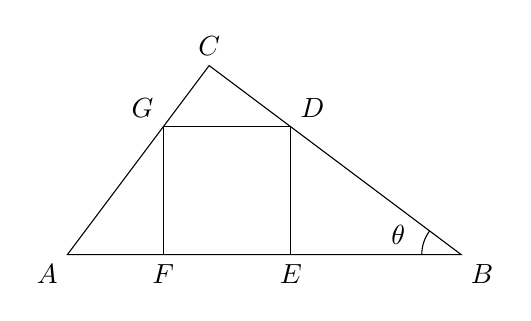
\begin{tikzpicture}[>=latex, line cap = round]
        \draw (0,0) node [below left] {$A$}-- (5,0) node [below right] {$B$}-- (9/5,12/5) node [above] {$C$}-- cycle;
        \draw (45/37,0) node [below] {$F$} -- (45/37,60/37) node [above left] {$G$}-- (105/37,60/37) node [above right] {$D$}-- (105/37,0) node [below] {$E$}; 
        \draw (5,0) ++ (180:0.5) arc (180:180-atan(3/4):0.5); 
        \draw (4.2,0) node [above] {$\theta$};
    \end{tikzpicture}
\end{center}
\item (003166)函数$y=2\sin(3x-\dfrac{\pi}4)$的图像的相邻两对称中心的距离是\blank{50}.
\item (003167)设$A>0$, $\omega>0$, $0\le \varphi<2\pi$. 如图为定义在$\mathbf{R}$上的函数$f(x)=A\sin (\omega x+\varphi)$的图像的一部分, 则$f(x)$的解析式为\blank{50}.
\begin{center}
    \begin{tikzpicture}[>=latex, line cap = round, scale = 0.8]
        \draw [->] (-1,0) -- (7,0) node [below] {$x$};
        \draw [->] (0,-3) -- (0,3) node [left] {$y$};
        \draw (0,0) node [below right] {$O$};
        \draw [domain = -pi/6:25*pi/12, samples = 1000] plot (\x, {2*sin(2*\x/3/pi*180+20)});
        \draw [dashed] (7*pi/12,2) -- (0,2) node [left] {$2$};
        \draw [dashed] (25*pi/12,0) node [above] {$\dfrac{25\pi}{12}$} --++ (0,-2) -- (0,-2) node [left] {$-2$};
        \draw (-pi/6,0) node [below] {$-\dfrac{\pi}{6}$};
    \end{tikzpicture}
\end{center}
\item (003168)要得到$y=\sin(\dfrac x2+\dfrac{\pi}4)$的图像, 可以将$y=\sin\dfrac x2$的图像\bracket{20}.
\fourch{向左平移$\dfrac{\pi}2$个单位}{向右平移$\dfrac{\pi}2$个单位}{向左平移$\dfrac{\pi}4$个单位}{向右平移$\dfrac{\pi}4$个单位}
\item (003169)把函数$y=\sin x$的图像上所有点向左平移$\dfrac{\pi}3$个单位长度, 再把所得图像上所有点的横坐标变为原来的$\dfrac 12$(纵坐标不变), 得到的图像是函数\blank{50}的图像.
\item (003170)若直线$x=a$与$f(x)=2\sin x$和$g(x)=3\cos x$的图像分别交于$M,N$两点, 则$|MN|$的最大值是\blank{50}.
\item (003171)设常数$\theta\in \mathbf{R}$. 函数$f(x)=\cos(x+\theta)$是偶函数, 当且仅当$\theta=$\blank{50}.
\item (003172)若函数$y=\tan \omega x$在$(-\dfrac{\pi}2,\dfrac{\pi}2)$上是减函数, 则实数$\omega$的取值范围是\blank{50}.
\item (003173)*设常数$t\in \mathbf{R}^+$. 若函数$y=-\sin (\dfrac{\pi }3x)$在区间$[0,t]$上恰好取得两次最大值, 则$t$的取值范围为\blank{50}.
\item (003174)设$f(x)=A\sin(\omega x+\varphi) \ (A>0, \ \omega>0, \ -\pi<\varphi<\pi)$, $D(2,\sqrt 2)$是图像的一个最高点, 一动点从$D$出发, 沿函数图像运动至相邻的最低点. 若$P$经过点$E(6,0)$, 求$f(x)$的解析式.
\item (003175)已知函数$f(x)=(2\sin(x+\dfrac{\pi}3)+\sin x)\cos x-\sqrt 3\sin^2 x$.\\
(1) 求函数$f(x)$的值域与周期;\\
(2) 若$x\in [0,\dfrac{\pi}2]$, 求$f(x)$的单调递减区间;\\
(3) *设常数$a>0$, 若函数$y=f(x)$的图像关于直线$x=a$对称, 求$a$的最小值;\\
(4) 设常数$m\in \mathbf{R}$, 若存在$x_0\in [0,\dfrac{5\pi}{12}]$, 使得$mf(x_0)-2=0$成立, 求$m$的取值范围.
\item (003176)设$A\ne 0$, $\omega>0$, $-\dfrac{\pi}2<\varphi<\dfrac{\pi}2$, 函数$f(x)=A\sin(\omega x+\varphi)$的部分图像如右图所示, 则$f(x)$的解析式为\blank{50}.
\begin{center}
    \begin{tikzpicture}[>=latex, line cap = round, scale = 0.4]
        \draw [->] (-4,0) -- (11,0) node [below] {$x$};
        \draw [->] (0,-5) -- (0,5) node [left] {$y$};
        \draw (0,0) node [below right] {$O$};
        \draw [domain = -2:11, samples = 1000] plot (\x, {-4*sin(180*\x/8+45)});
        \draw [dashed] (2,-4) -- (0,-4) node [left] {$-4$} (10,4) -- (0,4) node [left] {$4$};
        \draw (-2,0) node [above] {$-2$};
        \draw (6,0) node [below] {$6$};
    \end{tikzpicture}
\end{center}
\item (003177)函数$f(x)=\tan 2x$的图像的对称中心是\blank{50}.
\item (003178)函数$y=\sin(2x+\dfrac{\pi}4)$图像的对称轴可以是 \bracket{20}.
\fourch{$x=-\dfrac{3\pi}4$}{$x=-\dfrac{3\pi}8$}{$x=\dfrac{3\pi}8$}{$x=\dfrac{3\pi}4$}
\item (003179)与函数$y=\tan(2x+\dfrac{\pi}4)$没有公共点的直线可以是\bracket{20}.
\fourch{$x=-\dfrac{\pi}2$}{$x=-\dfrac{\pi}4$}{$x=\dfrac{\pi}8$}{$x=\dfrac{\pi}4$}
\item (003180)*设$\omega>0$, $0<\varphi <\pi$, 若函数$f(x)=\cos(\omega x+\varphi)$为奇函数, 且图像与直线$y=\dfrac 12$的所有交点中, 距离最近的两个交点的距离为$\pi$, 则$\omega =$\blank{50}, $\varphi=$\blank{50}.
\item (003181)*设常数$a\in \mathbf{R}$. 若函数$y=\sin 2x+a\cos 2x$的图像关于直线$x=-\dfrac{\pi}6$对称, 则$a=$\blank{50}.
\item (003182)*设常数$a\in \mathbf{R}$. 若关于$x$的方程$3\sin x+4\cos x=a$在区间$(0,2\pi)$内恰有两个相异实根$\alpha,\beta$, 求$a$的取值范围及$\alpha+\beta$的值.
\item (003183)求函数$y=\sin^4 x+2\sqrt 3\sin x\cos x-\cos^4 x$的最小正周期和值域, 写出该函数在$[0,\pi]$上的递增区间.
\item (003184)求值: $\arcsin\dfrac 12=$\blank{50}; $\arccos(-\dfrac{\sqrt 2}2)=$\blank{50}; $\arctan(-\sqrt 3)=$\blank{50}.
\item (003185)用含反三角函数的表达式表示下列各式中的角$x$:\\
(1) $\sin x=-\dfrac 13, \ x\in [-\dfrac{\pi}2,\dfrac{\pi}2]$, $x=$\blank{50};\\
(2) $\sin x=\dfrac 14, \ x\in [0,\pi]$, $x=$\blank{50};\\
(3) $\cos x=-\dfrac 14, \ x\in [0,\pi]$, $x=$\blank{50};\\ 
(4) $\cos x=\dfrac 15, \ x\in [-\pi,0]$, $x=$\blank{50};\\
(5) 三角形$ABC$中, $\sin A=\dfrac 14$, $\tan B=-2$, 则$A=$\blank{50}, $B=$\blank{50}.
\item (003186)设$|a|\le 1$, 则$\arccos a+\arccos(-a)=$\blank{50}.
\item (003187)化简下列各式: $\sin(\arcsin\dfrac 1{a^2+1})=$\blank{50}; $\cos(\arcsin(-\sqrt{1-a^4}))=$\blank{50}; $\cot(\arctan\dfrac 1a)=$\blank{50}.
\item (003188)函数$y=\sin x, \ x\in [-\dfrac{\pi}2,\dfrac{\pi}4]$的反函数是\blank{50}.
\item (003189)满足不等式$\arccos(1-x)\ge \arccos x$的$x$的取值范围是\blank{50}.
\item (003190)函数$y=(\arctan x)^2+\arctan x-1$的最小值是\blank{50}.
\item (003191)方程$2\sin x=1, \ x\in [-2\pi,2\pi]$的解集是\blank{50}.
\item (003192)研究函数$y=\arccos(x-x^2)$的定义域, 值域, 单调性, 并给出单调性的严格证明.
\item (003193)解下列三角方程:\\
(1) $\sin 2x=\sin 5x$;\\
(2) $\sin 2x-\sqrt 3\cos 2x=1, \ x\in [-\pi,\pi]$;\\
(3) $\dfrac{\sin 2x}{\cos x+\sin x}=4$;\\
(4) $\tan 2x=\tan 6x$;\\
(5) $\sin^2 x-4\sin x\cos x+2\cos^2 x=-\dfrac 12$.
\item (003194)下列等式成立的是\blank{50}(填序号).\\
\textcircled{1} $\arccos 0=1$; \textcircled{2} $\cos(\arccos \dfrac{\pi}2)=\dfrac{\pi}2$; \textcircled{3} $\sin(\arcsin\dfrac{\pi}4)=\dfrac{\pi}4$; 
\textcircled{4} $\arctan\dfrac{\pi}3=\sqrt 3$; \textcircled{5} $\tan(\arctan\dfrac{\pi}2)=\dfrac{\pi}2$.
\item (003195)若$\cos\alpha=-\dfrac 34$, $\alpha\in (\pi,\dfrac{3\pi}2)$, 则$\alpha=$\blank{50}.
\item (003196)设$x=\sin\alpha$, $\alpha\in (-\dfrac{\pi}6,\dfrac{5\pi}6]$, 则$\arccos x$的取值范围为\blank{50}.
\item (003197)方程$2\sin^2 x+5\sin x+2=0$在$(-2\pi,0)$上的解集为\blank{50}.
\item (003198)方程$2\sin^2 x-3\sin x\cos x-2\cos^2 x=0$的解集为\blank{50}.
\item (003199)若$\tan x=a, \ x\in (\dfrac{\pi}2,\pi)$, 则$x=$\blank{50}.
\item (003200)若$-\pi<x<-\dfrac{\pi}2$, 则$\arcsin(\sin x)=$\blank{50}.
\item (003201)设常数$m\in \mathbf{R}$, 关于$x$的方程$2-\sin 2x=m(2+\sin 2x), \ x\in [0,\pi)$的解集为$A$.\\
(1) 若$A\ne \varnothing$, 求$m$的取值范围;\\
(2) 若$A\subseteq (0,\pi)$, 且$A$中至少有两个元素, 求$m$的取值范围.
\item (003202)写出下列数列的一个通项公式:\\
(1) $-3,1,5,9,13,\cdots$: $a_n$=\blank{50}; (2)$\dfrac 27,\dfrac 4{11},\dfrac 12,\dfrac 45,2$: $a_n$=\blank{50}.
\item (003203)已知数列$\{a_n\}$满足: $a_n=n+\dfrac 6n$, 则数列$\{a_n\}$中最小项为第\blank{50}项.
\item (003204)(1) 数列$\{a_n\}$满足:  $a_1+a_2+a_3+\cdots +a_n=8$, 则$a_n=$\blank{50};\\
(2) 数列$\{a_n\}$满足:  $a_1\cdot a_2\cdot a_3\cdots a_n=8$, 则$a_n=$\blank{50}.
\item (003205)已知$a_1=1$, $a_2=3$, $a_{n+2}=a_{n+1}-a_n$, 则$a_{2030}=$\blank{50}.
\item (003206)数列$\{a_n\}$满足$a_{n+1}=\begin{cases}2a_n,&  0\le a_n<\dfrac 12,\\ 2a_n-1, &\dfrac 12\le a_n<1. \end{cases}$ 若$a_1=\dfrac 67$, 则$a_2=$\blank{50}; $a_3=$\blank{50}; $a_{2021}=$\blank{50}.
\item (003207)已知数列$\{a_n\}$和$\{b_n\}$, 其中$a_n=n^2$, $n\in \mathbf{N}^*$, $\{b_n\}$的项是互不相等的正整数, 若对于任意$n\in \mathbf{N}^*$, $\{b_n\}$的第$a_n$项等于$\{a_n\}$的第$b_n$项, 则$\dfrac{\lg (b_1b_4b_9b_{16})}{\lg (b_1b_2b_3b_4)}=$\blank{50}.
\item (003208)已知数列$\{a_n\}$的通项$a_n=n+\mathrm{e}^n$.\\
(1) 把该数列的前$10$项去掉, 得到新数列$\{b_n\}$, 则通项$b_n=$\blank{50};\\
(2) 将该数列的奇数项按原来的先后顺序排列, 得到新数列$\{c_n\}$, 则通项${c_n}=$\blank{50}.
\item (003209)已知数列$\{a_n\}$的前$n$项和是$S_n=2\cdot 3^n+3$, 求数列$\{a_n\}$的通项$a_n$.
\item (003210)已知数列$\{a_n\}$的通项$a_n=(n+1)(\dfrac{10}{11})^n$, 试问该数列有没有最大项? 若有, 求出最大项; 若没有, 说明理由.
\item (003211)已知$\{a_n\}$是递增数列, 且$a_n=n^2+\lambda n$, 求实数$\lambda$的取值范围.
\item (003212)已知数列$\{a_n\}$的通项$a_n=2^n$. 对任意的$k\in \mathbf{N}^*$, 在$a_{2k}$与$a_{2k+1}$中间插入一项$k$, 构成新数列$\{b_n\}:2,4,1,8,16,2,32,64,3,128,\cdots$. 求数列$\{b_n\}$的通项公式.
\item (003213)已知数列$\{a_n\}$满足$a_{n+2}=a_n$, ${a_1}=1$, ${a_2}=2$, 则通项$a_n=$\blank{50}.
\item (003214)已知数列$\{a_n\}$满足$a_{n+1}=a_n^2-k$, $a_1=1$, $a_3=-1$, 则常数$k=$\blank{50}.
\item (003215)已知数列$\{a_n\}$满足: $a_n=\dfrac 1{n-5.5}$, 则此数列中最大项的值为\blank{50}, 最小项的值为\blank{50}.
\item (003216)已知数列$\{a_n\}$满足: $a_n=2^n$, 删去数列中第$1,4,\cdots,3n-2,\cdots$项, 得到新数列的通项$b_n=$\blank{50}.
\item (003217)无穷数列$\{a_n\}$由$k$个不同的数组成, $S_n$为$\{a_n\}$的前$n$项和, 若对任意$n\in \mathbf{N}*$, $S_n\in \{2,3\}$, , 则$k$的最大值为\blank{50}.
\item (003218)设$\lambda$是实常数, 数列$\{a_n\}$的通项$a_n=n+\dfrac{\lambda}n$.\\
(1) 若数列$\{a_n\}$递增, 求$\lambda$的取值范围;\\
(2) 若数列$\{a_n\}$中, 唯一最小项为$a_4$, 求$\lambda$的取值范围.
\item (003219)已知正项数列$\{a_n\}$满足$a_n-\dfrac 1a_n=-2n$, 求证: 数列$\{a_n\}$是递减数列.
\item (003220)等差数列$\{a_n\}$中, 已知$a_1=3$, $d=2$, 则通项$a_n=$\blank{50}, 前$n$项和$S_n=$\blank{50}.
\item (003221)等差数列$\{a_n\}$中, 已知$a_1=3$, $a_2+a_5=-4$, $a_n=-11$, 则$n=$\blank{50}.
\item (003222)记等差数列$\{a_n\}$的前$n$项和为$S_n$, 若$a_3=0$, $a_7+a_8=0$, 则$S_7=$\blank{50}.
\item (003223)等差数列$\{a_n\}$中, 已知$a_1=1$, $a_1+a_2+a_5=13$, 则前$n$项和$S_n=$\blank{50}.
\item (003224)已知等差数列$\{a_n\}$的前$n$项之和为$S_n$, 若$S_{15}$为一确定常数, 则下列各式也为确定常数的是\bracket{20}.
\fourch{$a_2+a_{13}$}{$a_2\cdot a_{13}$}{$a_1+a_8+a_{15}$}{$a_1\cdot a_8\cdot a_{15}$}
\item (003225)在$a$和$b$($a<b$)之间插入$n$个数, 使这$n+2$个数组成递增的等差数列, 则该数列的公差为\blank{50}.
\item (003226)已知数列$\{a_n\}$的通项为$a_n=\sqrt{99}-n$, 前$n$项和为$S_n$, 则\\
(1) $\{a_n\}$中最后一个为正数的项是第\blank{50}项;\\
(2) 数列$\{S_n\}$中, 第\blank{50}项最大.
\item (003227)设数列$\{a_n\}$中, $a,b$为常数. 在下列三个条件中: \textcircled{1} $a_{n+1}-a_n=a$; \textcircled{2} $2a_{n+1}=a_n+a_{n+2}$; \textcircled{3} $a_n=an+b$, 可推出$\{a_n\}$是等差数列的条件为\blank{50}(填入序号).
\item (003228)已知数列$\{a_n\}$为等差数列, 公差为$d$. 求证: 数列$\{2a_{2n}\}$也是等差数列.
\item (003229)已知数列$\{a_n\}$的前$n$项和是$S_n=an^2+bn+c$, 其中$a,b,c$为常数, 若数列$\{a_n\}$为等差数列, 求实数$a,b,c$应满足的条件.
\item (003230)设等差数列$\{a_n\}$的前$n$项和为$S_n$, 已知$a_2=6$, $S_6>0$, $S_7<0$.\\
(1) 求公差$d$的取值范围;\\
(2) 数列$\{S_n\}$是否有最大项? 若有, 求出该项为第几项; 若无, 说明理由.
\item (003231)等差数列$\{a_n\}$中, $a_1+a_4+a_7=9$, $a_2+a_5+a_8=3$, 则$a_3+a_6+a_9=$\blank{50}.
\item (003232)设$S_n$为等差数列$\{a_n\}$的前n项和, 若$S_5=10$, $S_{10}=-5$, 则$S_{15}=$\blank{50}.
\item (003233)设$a$是实数, 若等差数列$\{a_n\}$的前$n$项和$S_n=n+a$, 则$a=$\blank{50}.
\item (003234)已知等差数列$\{a_n\}$, $\{b_n\}$的前$n$项和分别为$S_n,T_n$, 若$\dfrac{S_n}{T_n}=\dfrac{n-1}{n+1}$, 则$\dfrac{a_8}{b_8}=$\blank{50}.
\item (003235)等差数列$\{a_n\}$中, $S_n$为前$n$项和, 且$S_6<S_7$,$S_7>S_8$, 给出下列命题:\\
(1) 数列$\{a_n\}$中前$7$项是递增的, 从第$8$项开始递减;
(2) $S_9$一定小于$S_6$;
(3) $a_1$是$\{a_n\}$各项中的最大的;
(4) $S_7$不一定是$\{S_n\}$中最大项. 其中正确的序号是\blank{50}.
\item (003236)设等比数列$\{b_n\}$各项为正, 数列$\{a_n\}$满足: $a_n=\dfrac{\lg b_1+\lg b_2+\cdots+\lg b_n}n$, 证明: 数列 $\{a_n\}$为等差数列.
\item (003237)设数列$\{a_n\}$的通项公式为$a_n=pn+q$($n\in \mathbf{N}^*, \ p>0$). 数列$\{b_n\}$定义如下: 对于正整数$m$, $b_m$是使得不等式$a_n>m$成立的所有$n$中的最小值.\\
(1) 若$p=\dfrac{1}{2}$, $q=-\dfrac{1}{3}$求$b_3$;\\
(2) 若$p=2$, $q=-1$, 求数列$\{b_n\}$的前$2m$项和公式.
\item (003238)实数组成的等比数列$\{a_n\}$中, 已知$a_1=2$, $a_4=54$, 则通项$a_n=$\blank{50}.
\item (003239)等比数列$\{a_n\}$中, $a_1=4$, $a_2=2$, 则$a_1a_2+a_2a_3+\cdots +a_na_{n+1}=$\blank{50}.
\item (003240)已知数列$\{a_n\}$是等比数列, 且$a_n>0$, 若$b_n=\log_2a_n$, 则\bracket{20}
\twoch{$\{b_n\}$一定是递增的等差数列}{$\{b_n\}$不可能是等比数列}{$\{b_n+1\}$一定是等差数列}{$\{3^b_n\}$不是等比数列}
\item (003241)等比数列$\{a_n\}$满足$a_1=1$, $a_3=81$, 则$a_2=$\blank{50}.
\item (003242)若实数$a$、$b$、$c$、$d$、$e$依次构成等比数列, 且$a=-1$, $e=-81$, 则$c$=\blank{50}.
\item (003243)若等比数列$\{a_n\}$的前$n$项和为$S_n=3^n+a$, 则实数$a=$\blank{50}.
\item (003244)设等差数列$\{a_n\}$的前$n$项和为$S_n$, 则$S_4,S_8-S_4,S_{12}-S_8,S_{16}-S_{12}$成等差数列. 类比以上结论有: 设等比数列$\{b_n\}$的前$n$项积为$T_n$, 则$T_4$,\blank{50}, \blank{50}, $\dfrac{T_{16}}{T_{12}}$成等比数列.
\item (003245)几位大学生响应国家的创业号召, 开发了一款应用软件. 为激发大家学习数学的兴趣, 他们推出了``解数学题获取软件激活码''的活动. 这款软件的激活码为下面数学问题的答案: 已知数列$1, 1, 2, 1, 2, 4, 1, 2, 4, 8, 1, 2, 4, 8, 16, \cdots$, 其中第一项是$2^0$, 接下来的两项是$2^0,2^1$, 再接下来的三项是$2^0,2^1,2^2$, 依此类推.求满足如下条件的最小整数$N$($N>100$), 且该数列的前$N$项和为2的整数幂.那么该款软件的激活码是\bracket{20}.
\fourch{$440$}{$330$}{$220$}{$110$}
\item (003246)已知由实数组成的数列$\{a_n\}$, 前$n$项和记为$S_n$, 若数列$\{a_n\}$为等比数列, $S_{100}=100S_{50}$, 求$\dfrac{a_{100}}{a_{50}}$的值.
\item (003247)已知数列$\{c_n\}$, 其中$c_n=2^n+3^n$, 是否存在实数$p$使得数列$\{c_{n+1}-p{c_n}\}$为等比数列, 若存在, 求出$p$; 若不存在, 说明理由.
\item (003248)已知等比数列$\{a_n\}$中每一项均为实数, 设数列$\{a_n\}$的前$n$项和为$S_n$.\\
(1) 证明: $(S_{2n}-S_n)^2=S_n(S_{3n}-S_{2n})$;\\
(2) 试给出一个例子使得$S_n,S_{2n}-S_n,S_{3n}-S_{2n}$依次不构成等比数列;\\
(3) 若$S_{10}=2$, $S_{30}=14$, 求$S_{20}$.
\item (003249)等比数列$\{a_n\}$满足$a_1=2$, $a_2=1$, 则通项$a_n=$\blank{50}.
\item (003250)若等比数列$\{a_n\}$的公比为$3$, 则等比数列$\{a_n\cdot a_{n+3}\}$的公比为\blank{50}.
\item (003251)若实数$a$使得$a,a^2,a$依次构成等比数列, 则$a=$\blank{50}.
\item (003252)若数列$\{a_n\}$为等差数列, 则$a_9=4a_3-3a_1$. 类比以上结论有: 若数列$\{b_n\}$为等比数列, 则$b_9=$\blank{50}.
\item (003253)设$\{a_n\}$是各项为正数的无穷数列, $A_i$是边长为$a_i$、$a_{i+1}$的矩形的面积($i=1,2,\cdots$), 则$\{a_n\}$为等比数列的充要条件是\bracket{20}.
\onech{$\{a_n\}$是等比数列}{$a_1,a_3,\cdots,a_{2n-1},\cdots$或$a_2,a_4,\cdots,a_{2n},\cdots$是等比数列}{$a_1,a_3,\cdots,a_{2n-1},\cdots$和$a_2,a_4,\cdots,a_{2n},\cdots$均是等比数列}{$a_1,a_3,\cdots,a_{2n-1},\cdots$和$a_2,a_4,\cdots,a_{2n},\cdots$均是等比数列, 且公比相同}
\item (003254)设$p\in \mathbf{R}$, 已知数列$\{a_n\}$满足$a_1=1$, $a_{n+1}=a_n^2-p$, 是否存在$p$使得$\{a_n\}$是等比数列? 若存在, 求出$p$的值; 若不存在, 说明理由.
\item (003255)设数列$\{a_n\}$的前$n$项和为$S_n$, 已知$a_1=1$, $S_{n+1}=4a_n+2$.\\
(1) 设$b_n=a_{n+1}-2a_n$, 证明数列$\{b_n\}$是等比数列;\\
(2) 求数列$\{a_n\}$的通项公式.
\item (003256)求和: $\sin^21^\circ +\sin^22^\circ+\sin^23^\circ+\cdots+\sin^288^\circ+\sin^289^\circ=$\blank{50}.
\item (003257)设$f(x)=\dfrac 1{3^x+\sqrt 3}$, 利用课本中推导等差数列前$n$项和的公式的方法, 可求得$f(-5)+f(-4)+\cdots+f(0)+\cdots+f(5)+f(6)$的值为\blank{50}.
\item (003258)已知数列$\{a_n\}$的通项$a_n=1+2+2^2+\cdots+2^n$, 则其前$n$项和$S_n=$\blank{50}.
\item (003259)已知数列$\{a_n\}$的通项$a_n=\dfrac 1{(2n-1)(2n+1)}$, 则其前$n$项和$S_n=$\blank{50}.
\item (003260)已知数列$\{a_n\}$的通项$a_n=\dfrac 3{n(n+3)}$, 则其前$n$项和$S_n$=\blank{50}.
\item (003261)等比数列$\{a_n\}$中前$n$项和为$S_n$, $n\in \mathbf{N}^*$, 若$S_n=48$, $S_{2n}=60,$则$S_{4n}=$\blank{50}.
\item (003262)在等差数列$\{a_n\}$中, 满足$3a_4=7a_7$, 且$a_1>0$, $S_n$是数列$\{a_n\}$前$n$项的和, 若$S_n$取得最大值, 则$n=$\blank{50}.
\item (003263)已知数列$\{a_n\}$的通项$a_n=n\cdot 2^n$, 求其前$n$项和$S_n$.
\item (003264)已知数列$\{a_n\}$的前$n$项和为$S_n=n^2-20n$, 求数列$\{|a_n|\}$的前$n$项和$T_n$.
\item (003265)求数列$\{\dfrac{(n+1)^2+1}{(n+1)^2-1}\}$的前$n$项和$S_n$.
\item (003266)(1) 设$n$为正整数, 求和: $1-3+5-7+9+\cdots +(-1)^{n-1}\cdot (2n-1)$;\\
(2) 已知数列$\{a_n\}$的通项$a_n=\begin{cases}3n+1, & n\text{为奇数}, \\ 2^{\frac n2}, & n\text{为偶数},  \end{cases}$ 求其前$n$项和$S_n$.
\item (003267)数列$\{a_n\}$的通项$a_n=2^n\cdot 3^n$, 则其前$n$项和$S_n=$\blank{50}.
\item (003268)已知数列$\{a_n\}$的通项$a_n=\dfrac 2{\sqrt{n+2}+\sqrt n}$, 则其前$n$项和$S_n=$\blank{50}.
\item (003269)等差数列$\{a_n\}$的前$n$项和为$S_n$, $a_3=3$, $S_4=10$, 则数列$\{S_n\}$的前$n$项和为\blank{50}.
\item (003270)求数列$\{\dfrac n{2^n}\}$的前$n$项和$S_n$.
\item (003271)已知数列$\{a_n\}$满足$a_n=\begin{cases}n, & n
\text{是奇数}, \\ 2^n, & n\text{是偶数}. \end{cases}$ 试求数列$\{a_n\}$的前$n$项和$S_n$.
\item (003272)如果有穷数列$a_1,a_2,a_3,\cdots,a_m$($m$为正整数)满足条件$a_1=a_m$, $a_2=a_{m-1}$, $\cdots$, $a_m=a_1$, 即$a_i=a_{m-i+1}$($i=1,2,\cdots,m$), 我们称其为``对称数列''.  例如数列$1,2,5,2,1$与数列$8,4,2,2,4,8$都是``对称数列''.\\
(1) 设$\{c_n\}$是$49$项的``对称数列'', 其中$c_{25},c_{26},\cdots,c_{49}$是首项为$1$, 公比为$2$的等比数列, 求$\{c_n\}$各项的和$S$;\\
(2) 设$\{d_n\}$是$100$项的``对称数列'', 其中$d_{51},d_{52}\cdots,d_{100}$是首项为$2$, 公差为$3$的等差数列. 求$\{d_n\}$前$n$项的和$S_n$($n=1,2,\cdots,100$).
\item (003273)设数列$\{a_n\}$满足$a_1=0$且$\dfrac 1{1-a_{n+1}}-\dfrac 1{1-a_n}=1$.\\
(1) 求$\{a_n\}$的通项公式;\\
(2) 设$b_n=\dfrac{1-\sqrt{a_{n+1}}}{\sqrt n}$, 记$S_n={b_1}+{b_2}+\cdots +b_n$, 求$\{S_n\}$的通项公式.
\item (003274)数学归纳法证明$1+a+a^2+\cdots+a^{n+1}=\dfrac{1-a^{n+2}}{1-a}\ (a\ne 1)$, 在验证$n=1$时, 左边计算所得项为\blank{50}.
\item (003275)用数学归纳法证明``对于任意正偶数$n$, $a^n-b^n$能被$a+b$整除''时, 其第二步论证应该是\bracket{20}.
\onech{假设$n=k$, $k\in \mathbf{N}^*$时命题成立, 证明$n=k+1$时, 命题也成立}{假设$n=2k$, $k\in \mathbf{N}^*$时命题成立, 证明$n=2k+1$时, 命题也成立}{假设$n=k$, $k\in \mathbf{N}^*$时命题成立, 证明$n=k+2$时, 命题也成立}{假设$n=2k$, $k\in \mathbf{N}^*$时命题成立, 证明$n=2k+2$时, 命题也成立}
\item (003276)用数学归纳法证明: $1^2-2^2+3^2-4^2+\cdots+(2n-1)^2-(2n)^2=-n(2n+1)$, $n$从$k$到$k+1$时, 等式左边增加的项为\blank{50}.
\item (003277)根据$1=1$, $1-4=-(1+2)$, $1-4+9=1+2+3$, $1-4+9-16=-(1+2+3+4)$, $\cdots$, 请写一个能体现其一般规律的数学表达式:\blank{50}.
\item (003278)设$f(x)$是定义在正整数集上的函数, 且$f(x)$满足: ``当$f(k)\ge k^2$成立时, 总可推出$f(k+1)\ge (k+1)^2$成立''. 那么, 下列说法中正确的是\bracket{20}.
\onech{若$f(3)\ge 9$成立, 则当$k\ge 1$时, 均有$f(k)\ge k^2$成立}{若$f(5)\ge 25$成立, 则当$k\le 5$时, 均有$f(k)\ge k^2$成立}{若$f(7)<49$成立, 则当$k\ge 8$时, 均有$f(k)<k^2$成立}{若$f(4)=25$成立, 则当$k\ge 4$时, 均有$f(k)\ge k^2$成立 }
\item (003279)已知数列$\{a_n\}$满足$a_1=2$, $a_{n+1}=\dfrac{1-a_n}{1+a_n}$, 则$\{a_n\}$的通项$a_n=$\blank{50}.
\item (003280)已知数列$\{a_n\}$满足$a_1=1$, $a_{n+1}=n+\dfrac 2{a_n-n+2}$, 猜测$\{a_n\}$的通项, 并用数学归纳法证明.
\item (003281)是否存在实数$a$, 使得等式$\dfrac 1{1^2}+\dfrac 1{2^2}+\cdots +\dfrac 1{n^2}=\dfrac{an}{3n-1}$对一切正整数$n$成立? 请说明理由.
\item (003282)用数学归纳法证明: 对一切正整数$n$, $5^n+12n-1$是$16$的倍数.
\item (003283)正数数列$\{a_n\}$前$n$项和为$S_n$, 若$S_n=\dfrac 12(a_n+\dfrac 1{a_n})$.\\
(1) 求$a_1,a_2,a_3$的值;\\
(2) 猜测通项$a_n$, 并用数学归纳法加以证明.
\item (003284)数学归纳法证明: $1-\dfrac 12+\dfrac 13-\dfrac 14+\cdots +\dfrac 1{2n-1}-\dfrac 1{2n}=\dfrac 1{n+1}+\dfrac 1{n+2}+\cdots +\dfrac 1{2n}$时, 当$n$从$k$到$k+1$时等式右边增加与减少的项分别为\blank{50}, \blank{50}.
\item (003285)若$S_n=1+\dfrac 12+\dfrac 13+\cdots +\dfrac 1n$, 用数学归纳法证明: $S_{2^n}>1+\dfrac n2\ (n\ge 2)$, $n$从$k$到$k+1$时, 不等式左边增加的项为\blank{50}.
\item (003286)根据 $1=1$, $2+3+4=9$, $3+4+5+6+7=25$, $\cdots$, 请写一个能体现其一般规律的数学表达式:\blank{50}.
\item (003287)(1) 已知数列$\{a_n\}$满足$a_1=3$, $a_{n+1}=a_n^2-2\ (n\in \mathbf{N}^*)$. 求证: 当$n\in \mathbf{N}^*$时, $a_n\ge 3$;\\
(2) *已知数列$\{a_n\}$满足$a_n\ge 0$, $a_1=0$, $a_{n+1}^2+a_{n+1}-1=a_n^2 \ (n\in \mathbf{N}^*)$. 求证: 当$n\in \mathbf{N}^*$时, $a_n<a_{n+1}$.
\item (003288)在数列$\{a_n\}$, $\{b_n\}$中, $a_1=2$, $b_1=4$, 且$a_n,b_n,a_{n+1}$成等差数列, $b_n,a_{n+1},b_{n+1}$成等比数列($n\in \mathbf{N}^*)$. 写出$a_2,a_3,a_4$及$b_2,b_3,b_4$的值, 由此猜测$\{a_n\}$, $\{b_n\}$的通项公式, 并证明你的结论.
\item (003289)(1) 用数学归纳法证明: 对一切正整数$n$, $2^{n+2}\cdot 3^n+5n+21$能被$25$整除;\\
(2) *是否存在大于$1$的正整数$m$, 使得对于任意正整数$n$, $f(n)=(2n+7)\cdot 3^n+9$都能被$m$整除? 若存在, 求出$m$的最大值, 并证明你的结论; 若不存在, 说明理由.
\item (003290)数列$\{a_n\}$中, $a_n=\begin{cases}\dfrac 1{n^2}, & 1\le n\le 10^{10},  \\ \dfrac{2020n^2}{2020n^2-2022n}, & n\ge 10^{10},\end{cases}$ 则数列$\{a_n\}$的极限值\bracket{20}.
\fourch{等于$0$}{等于$1$}{等于$0$或$1$}{不存在}
\item (003291)(1) $\displaystyle\lim_{n\to \infty}(\dfrac{n^2+1}n-\dfrac{n^2}{n+1})=$\blank{50};\\
(2) 设$m\in \mathbf{N}^*$, 则$\displaystyle\lim_{n\to \infty}(\dfrac mn-\dfrac 1{n+1}-\dfrac 1{n+2}-\dfrac 1{n+3}-\cdots -\dfrac 1{n+m})=$\blank{50}.
\item (003292)设等比数列$\{a_n\}$的通项公式为$a_n={q^{n+1}}$($n\in \mathbf{N}^*$), 前$n$项和为$S_n$.若$\displaystyle\lim_{n\to \infty}\dfrac {S_n}{a_{n+1}}=\dfrac 12$, 则$q$=\blank{50}
\item (003293)设$a$是实常数, 则:\\
(1) $\displaystyle\lim_{n\to \infty}\dfrac{2an^2+n+1}{an^2-n+1}=$\blank{50};\\
(2) $\displaystyle\lim_{n\to \infty}\dfrac{1-2a^n}{1+a^n}=$\blank{50}($a\ne -1$).
\item (003294)无穷等比数列$\{a_n\}$的前$n$项和为$S_n$, 则数列$\{a_n\}$有极限是数列$\{S_n\}$有极限的\bracket{20}条件.
\fourch{充分不必要}{必要不充分}{充要}{既不充分又不必要}
\item (003295)化简: $0.\dot1\dot6=$\blank{50}; $0.1\dot6$=\blank{50};
 $0.1\dot6+0.01\dot6+0.001\dot6+\cdots$=\blank{50}(用最简分数表示)
.
\item (003296)如图, 正方形$ABCD$边长为1, 联结该正方形各边的中点得到一个新的正方形$A_1B_1C_1D_1$, 再在正方形$A_1B_1C_1D_1$中用同样的方法得到又一个新的正方形$A_2B_2C_2D_2$, 这样无限地继续下去, 则所有这些得到的新正方形面积之和为\blank{50}.
\begin{center}
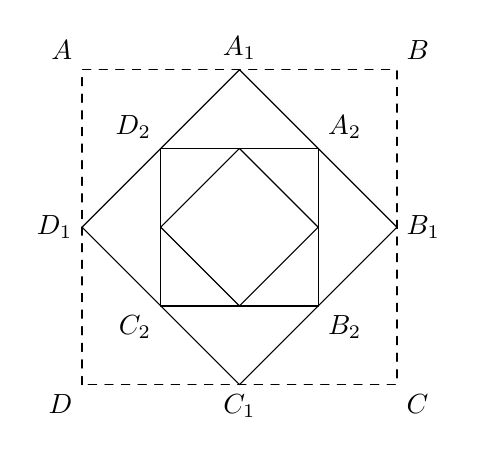
\begin{tikzpicture}[>=latex, line cap = round, line join = round]
    \draw [dashed] (0,0) rectangle (4,4);
    \draw (0,2) -- (2,4) -- (4,2) -- (2,0) -- cycle;
    \draw (1,3) -- (3,3) -- (3,1) -- (1,1) -- cycle;
    \draw (2,3) -- (3,2) -- (2,1) -- (1,2) -- cycle;
    \draw (0,4) node [above left] {$A$} (4,4) node [above right] {$B$} (4,0) node [below right] {$C$} (0,0) node [below left] {$D$};
    \draw (2,4) node [above] {$A_1$} (4,2) node [right] {$B_1$} (2,0) node [below] {$C_1$} (0,2) node [left] {$D_1$};
    \draw (3,3) node [above right] {$A_2$} (3,1) node [below right] {$B_2$} (1,1) node [below left] {$C_2$} (1,3) node [above left] {$D_2$};
\end{tikzpicture}
\end{center}
\item (003297)已知公比为$q(0<q<1)$的无穷等比数列$\{a_n\}$各项的和为$9$, 无穷等比数列$\{a_n^2\}$各项的和为$\dfrac{81}5$.则数列$\{a_n\}$的首项$a_1=$\blank{50}, 公比$q$=\blank{50}.
\item (003298)已知$a_n=\begin{cases} \dfrac 1{2^n}, & n\text{为奇数}, \\ \dfrac 1{3^n}, & n\text{为偶数}, \end{cases}$ 求$\displaystyle\lim_{n\to \infty}(a_1+a_2+\cdots +a_{2n})$.
\item (003299)已知$a,b,c$是实数, $\displaystyle\lim_{n\to \infty}\dfrac{an+1}{bn+3}=\dfrac 13$, $\displaystyle\lim_{n\to \infty}\dfrac{bn^2-4}{cn^2+2}=-2$. 求$\displaystyle\lim_{n\to \infty}\dfrac{an^3+2n+5}{cn^3+4n+3}$.
\item (003300)设$\{a_n\}$是首项为$a$, 公比为$q(q>0)$的等比数列, 前$n$项和为$S_n$, 若$G_n=a_1^2+a_2^2+\cdots+a_n^2$, 求$\displaystyle\lim_{n\to \infty}\dfrac{S_n}{G_n}$.
\item (003301)设无穷等比数列$\{a_n\}$满足$\displaystyle\lim_{n\to \infty}(a_1+a_3+a_5+\cdots +a_{2n-1})=\dfrac 83$, 则首项$a_1$的取值范围为\blank{50}.
\item (003302)(1) $\displaystyle\lim_{n\to \infty}\dfrac{(-2)^n+1}{(-2)^{n+1}+1}$=\blank{50};\\
(2) $\displaystyle\lim_{n\to \infty}\dfrac{6-2+4-8+\cdots+(-2)^{n+1}}{4+3+9+27+\cdots+3^n}$=\blank{50}.
\item (003303)(1)若$\displaystyle\lim_{n\to \infty}(\dfrac{n^3-1}{2n^2+n}-an-b)=0$, 则$a$=\blank{50}, $b$=\blank{50};\\
(2) 若$\displaystyle\lim_{n\to \infty}\dfrac{5^n}{5^{n+1}+(a+1)^n}=\dfrac 15$, 则实数$a$的取值范围是\blank{50}.
\item (003304)设$\{a_n\}$为无穷等比数列, 若$\{a_n\}$的任意一项都是它后面所有项和的$4$倍, 则公比为\blank{50}.
\item (003305)已知无穷等比数列$\{a_n\}$的公比为$q$, 前$n$项和为$S_n$, 且$\displaystyle\lim_{n\to \infty}S_n=S$, 下列条件中, 使得$2S_n<S$($n\in \mathbf{N}*$)恒成立的是\bracket{20}.
\twoch{$a_1>0,\ 0.6<q<0.7$}{$a_1<0,\ -0.7<q<-0.6$}{$a_1>0, \ 0.7<q<0.8$}{$a_1<0,\ -0.8<q<-0.7$}
\item (003306)设等差数列$\{a_n\}$的公差为$d$, 若$a_n$恒不为零, 求$\displaystyle\lim_{n\to \infty}\dfrac{S_n}{na_n}$.
\item (003307)已知等差数列$\{a_n\}$的首项为$1$, 公差为$d$, 前$n$项的和为$A_n$; 等比数列的首项为$1$, 公比为$q$, $|q|<1$, 前$n$项的和为$B_n$, 记$S_n=B_1+B_2+\cdots+B_n$, 若$\displaystyle\lim_{n\to \infty}(\dfrac{a_n}n-S_n)=1$, 求$d$、$q$.
\item (003308)已知数列$\{a_n\}$是公差不为$0$的等差数列, $a_1=\dfrac 12$, 数列$\{b_n\}$是等比数列, 且$b_1=a_1$, $b_2=a_3$, $b_3=a_4$. 数列$\{b_n\}$的前$n$项和为$S_n$, 记点${Q_n}(b_n,S_n)$, $n\in \mathbf{N}*$.\\
(1) 求数列$\{b_n\}$的通项公式;\\
(2) 证明点$Q_1,Q_2,\cdots,Q_n,\cdots$在同一条直线$l$上, 并求出直线$l$的方程;\\
(3) 若记$\triangle OQ_nQ_{n+1}$($n\in \mathbf{N}*$)的面积为$a_n$, 且${T_n}$为数列$\{a_n\}$的前$n$项和, 求$\displaystyle\lim_{n\to \infty}a_n$、$\displaystyle\lim_{n\to \infty}T_n$.
\item (003309)数列$\{a_n\}$满足: $a_1=1$, $a_{n+1}=a_n+2^n$, 则$a_n=$\blank{50}.
\item (003310)数列$\{a_n\}$满足: $a_1=1$, $a_{n+1}=2^na_n$, 则$a_n=$\blank{50}.
\item (003311)数列$\{a_n\}$满足: $a_1=2$, $a_{n+1}=\sqrt a_n$, 则$a_n=$\blank{50}.
\item (003312)数列$\{a_n\}$满足: $a_1=3$, $a_{n+1}=4a_n+6$, 则$a_n=$\blank{50}.
\item (003313)数列$\{a_n\}$及前$n$项和$S_n$满足: $S_n=2a_n+n-4$, 则$a_n$=\blank{50}.
\item (003314)数列$\{a_n\}$及前$n$项和$S_n$满足: $a_1=3$, $S_{n-1}=a_n+n$, $n\ge 2$, 则$a_n=$\blank{50}.
\item (003315)数列$\{a_n\}$满足: $a_1=1$, $a_{n+1}=\dfrac{2a_n}{a_n+4}$, 则$a_n=$\blank{50}.
\item (003316)已知数列$\{a_n\}$满足$a_1=3$, $a_n\times a_{n+1}=(\dfrac 12)^n$, 求此数列的通项$a_n$.
\item (003317)数列$\{a_n\}$满足$a_1=\dfrac 35$, $a_n=2-\dfrac 1{a_{n-1}}$, 数列$\{b_n\}$满足$b_n=\dfrac 1{a_n-1}$.\\
(1) 求证: 数列$\{b_n\}$是等差数列;\\
(2) 求数列$\{a_n\}$的通项.
\item (003318)数列$\{a_n\}$的首项为$\dfrac 12$, 且前$n$项和$S_n$和$a_n$满足: 当$n\ge 2$时, $S_n^2=a_n(S_n-1)$, 求$a_n$、$S_n$.
\item (003319)已知数列$\{a_n\}$满足$a_1=1$, $a_{n+1}+a_n=8$, 则通项$a_n=$\blank{50}.
\item (003320)已知数列$\{a_n\}$满足$a_1=1$, $a_n=a_1+2a_2+3a_3+\cdots+(n-1)a_{n-1}$, $n\ge 2$, 则通项$a_n=$\blank{50}.
\item (003321)已知数列$\{a_n\}$满足$a_n=\begin{cases} 5, & n=1, \\ a_1+a_2+...+a_{n-1}, & n\ge 2. \end{cases}$ 则通项$a_n=$\blank{50}.
\item (003322)已知数列$\{a_n\}$满足: $a_1=3$, $a_{n+1}=-2a_n+6$, 求$a_n$.
\item (003323)数列$\{a_n\}$中, $a_1=1$, $a_2=2$, 且$a_{n+1}=(1+q)a_n-qa_{n-1}$($n\ge 2, \ q\ne 0$).\\
(1) 设$b_n={a_{n+1}}-a_n$($n\in \mathbf{N}^*$), 证明$\{b_n\}$是等比数列;\\
(2) 求数列$\{a_n\}$的通项公式.
\item (003324)设数列$\{a_n\}$的前$n$项和为$S_n$, 满足$6S_n=(a_n+1)(a_n+2)$.\\
(1) 若$a_n>0$, 求通项$a_n$;
(2) (不需要理由)试写出所有可能的数列$\{a_n\}$的前三项.
\item (003325)已知数列$\{a_n\}$和$\{b_n\}$满足: $a_1=\lambda$, $a_{n+1}=\dfrac 23a_n+n-4$, $b_n=(-1)^n(a_n-3n+21)$, 其中$\lambda$为实数.\\
(1) 对任意实数$\lambda$, 证明数列$\{a_n\}$不是等比数列;\\
(2) *若数列$\{b_n\}$是等比数列, 求$\lambda$的取值范围;\\
(3) *若$a_n<3n$对一切$n\in \mathbf{N}^*$成立, 求$\lambda$的取值范围.
\item (003326)若$OEF$是不共线的任意三点, 则以下各式中成立的是\bracket{20}.
\twoch{$\overrightarrow{EF}=\overrightarrow{OF}+\overrightarrow{OE}$	}{$\overrightarrow{EF}=\overrightarrow{OF}-\overrightarrow{OE}$	 }{$\overrightarrow{EF}=-\overrightarrow{OF}+\overrightarrow{OE}$	 }{$\overrightarrow{EF}=-\overrightarrow{OF}-\overrightarrow{OE}$}
\item (003327)已知$\overrightarrow a$、$\overrightarrow b$、$\overrightarrow c$为非零向量, 下列命题中假命题是\blank{50}.\\
(1) $\overrightarrow a+(-\overrightarrow a)=0$;\\
(2) 若$| \overrightarrow a|=|\overrightarrow b|$, 则$\overrightarrow a=\overrightarrow b$或$\overrightarrow a=-\overrightarrow b$;\\
(3) $\overrightarrow a\parallel \overrightarrow b$是$| \overrightarrow a+\overrightarrow b|=|\overrightarrow a|+|\overrightarrow b|$成立的充分非必要条件;\\
(4) $\overrightarrow a+\overrightarrow b+\overrightarrow c=\overrightarrow 0$是$\overrightarrow a$、$\overrightarrow b$、$\overrightarrow c$可以首尾相接构成三角形的必要非充分条件.
\item (003328)设$\overrightarrow m$、$\overrightarrow n$为非零向量, 则``存在负数$\lambda$, 使得$\overrightarrow m=\lambda \overrightarrow n$''是``$\overrightarrow m\cdot \overrightarrow n<0$''的\bracket{20}.
\twoch{充分而不必要条件}{必要而不充分条件}{充分必要条件}{既不充分也不必要条件}
\item (003329)若$\overrightarrow{P_1O}=-3\overrightarrow{OP_2}$, 则$\overrightarrow{P_1P_2}=$\blank{50}$\overrightarrow{P_2O}$.
\item (003330)已知$\triangle ABC$中, $AB=2$, $AC=3$, $\angle A=120^\circ$, 设$\overrightarrow a=\overrightarrow{AB},\overrightarrow b=\overrightarrow{AC}$, 用$\overrightarrow a,\overrightarrow b$表示$\overrightarrow{BC}$的单位向量为\blank{50};$|\overrightarrow a+\overrightarrow b|=$\blank{50}.
\item (003331)若$|\overrightarrow{AB}|=8$, $|\overrightarrow{AC}|=9$, 则$|\overrightarrow{BC}|$的取值范围是\blank{50}.
\item (003332)已知向量$\overrightarrow a$、$\overrightarrow b$是单位向量, $\overrightarrow a\cdot \overrightarrow b=0$, 且向量$\overrightarrow c$满足$|\overrightarrow c-\overrightarrow a-\overrightarrow b|=1$, 则$|\overrightarrow c|$的取值范围是\bracket{20}.
\fourch{$[\sqrt 2-1,\sqrt 2+1]$}{$[\sqrt 2-1,\sqrt 2]$}{$[\sqrt 2,\sqrt 2+1]$}{$[2-\sqrt 2,2+\sqrt 2]$}
\item (003333)若平面上三点$A,B,C$共线, $O$是直线$AB$外一点, 且$\overrightarrow{OC}=\lambda \overrightarrow{OA}+\mu \overrightarrow{OB}$($\lambda,\mu \in \mathbf{R}$), 求$\lambda +\mu$的值.
\item (003334)已知$|\overrightarrow a+\overrightarrow b|=2| \overrightarrow a-\overrightarrow b|$, $|\overrightarrow a|=1$, $|\overrightarrow b|=2$. 求:\\
(1) $|3\overrightarrow a-2\overrightarrow b|$;\\
(2) $\overrightarrow a$与$\overrightarrow a+\overrightarrow b$的夹角;\\
(3) $\overrightarrow a$在$\overrightarrow a+\overrightarrow b$方向上的投影.
\item (003335)已知$|\overrightarrow{a}|$=$\sqrt 2$, $|\overrightarrow{b}|=3$, $\overrightarrow{a}$和$\overrightarrow{b}$的夹角为$45^\circ$, 求当向量$\overrightarrow{a}+\lambda \overrightarrow{b}$与$\lambda \overrightarrow{a}+\overrightarrow{b}$夹角为锐角时, 求 $\lambda$的取值范围.
\item (003336)若点$O$是$\triangle ABC$内一点, $\overrightarrow{OA}+\overrightarrow{OB}+\overrightarrow{OC}=\overrightarrow 0$, 则点$O$是$\triangle ABC$的\blank{50}心.
\item (003337)在平行四边形$ABCD$中, $AC$与$BD$交于点$O$, $E$是线段$OD$的中点, $AE$的延长线与$CD$交于点$F$. 若$\overrightarrow{AC}=\overrightarrow a$, $\overrightarrow{BD}=\overrightarrow b$, 则$\overrightarrow{AF}=$\blank{50}.
\begin{center}
    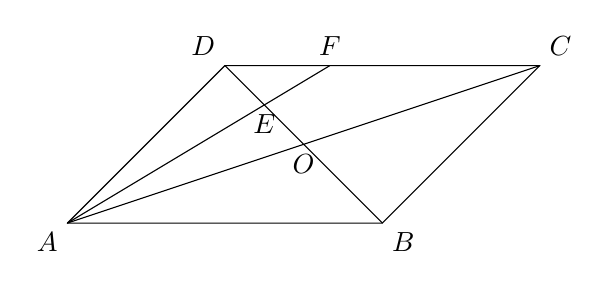
\begin{tikzpicture}[>=stealth, line cap = round, line join = round, scale = 2]
        \draw (0,0) node [below left] {$A$} -- (2,0) node [below right] {$B$}-- (3,1) node [above right] {$C$} -- (1,1) node [above left] {$D$}-- cycle;
        \draw (0,0) -- (3,1) (2,0) -- (1,1);
        \draw (0,0) -- (5/3,1) node [above] {$F$};
        \draw (1.5,0.5) node [below] {$O$};
        \draw (1.25,0.75) node [below] {$E$};
    \end{tikzpicture}
\end{center}
\item (003338)平面上点$ABC$满足$|\overrightarrow{AB}|=3$, $|\overrightarrow{BC}|=4$, $|\overrightarrow{CA}|=5$, 则$\overrightarrow{AB}\cdot \overrightarrow{BC}+\overrightarrow{BC}\cdot \overrightarrow{CA}+\overrightarrow{CA}\cdot \overrightarrow{AB}$=\blank{50}.
\item (003339)在$\triangle ABC$中, $\angle A=60^\circ$, $AB=3$, $AC=2$. 若$\overrightarrow{BD}=2\overrightarrow{DC}$, $\overrightarrow{AE}=\lambda \overrightarrow{AC}-\overrightarrow{AB}$, 且$\overrightarrow{AD}\cdot \overrightarrow{AE}=-4$, 则$\lambda$的值为\blank{50}.
\item (003340)$\overrightarrow a$、$\overrightarrow b$是非零向量且满足$(\overrightarrow a-2\overrightarrow b)\perp \overrightarrow a$, $(\overrightarrow b-2\overrightarrow a)\perp \overrightarrow b$, 则$\overrightarrow a$与$\overrightarrow b$的夹角是\blank{50}.
\item (003341)(1) 已知$\overrightarrow a$与$\overrightarrow b$都是非零向量, 且$|\overrightarrow a|=|\overrightarrow b|=|\overrightarrow a-\overrightarrow b|$, 求$\overrightarrow a$与$\overrightarrow a+\overrightarrow b$的夹角;\\
(2) 已知向量$\overrightarrow a$与$\overrightarrow b$的夹角为$120^\circ$, $|\overrightarrow a|=3,|\overrightarrow a+\overrightarrow b|=\sqrt{13}$, 求$|\overrightarrow b|$的值.
\item (003342)*已知向量$\overrightarrow a$、$\overrightarrow b$满足$| \overrightarrow a|=1$, $|\overrightarrow{b}|=2$, 求$|\overrightarrow a+\overrightarrow b|+|\overrightarrow a-\overrightarrow b|$的最小值、最大值.
\item (003343)若$\overrightarrow{AB}=(2,4)$, $\overrightarrow{AC}=(1,3)$, 则$\overrightarrow{BC}$方向相反的单位向量是\blank{50}.
\item (003344)已知点$P_1(2,-1)$、$P_2(0,5)$, 若点$P$在直线$P_1P_2$上, 且满足$|\overrightarrow{P_1P_2}|=2|\overrightarrow{PP_2}|$, 则点$P$的坐标为\blank{50}.
\item (003345)若三点$A(2,2)$、$B(a,0)$、$C(0,4)$共线, 则$a$的值等于\blank{50}.
\item (003346)已知$\overrightarrow{e_1},\overrightarrow{e_2}$是不平行的向量, 设$\overrightarrow a=\overrightarrow {e_1}+k\overrightarrow {e_2}$, $\overrightarrow b=k\overrightarrow {e_1}+\overrightarrow {e_2}$, 则$\overrightarrow a$与$\overrightarrow b$平行的充要条件是实数$k$等于\blank{50}.
\item (003347)已知向量$\overrightarrow a=(1,2)$, $\overrightarrow b=(0,3)$, 则与$\overrightarrow a$垂直的单位向量的坐标为\blank{50}; $\overrightarrow b$在$\overrightarrow a$的方向上的投影为\blank{50}.
\item (003348)已知$\triangle ABC$的三个顶点分别是$A(1,\dfrac 32)$, $B(4,-2)$, $C(1,y)$, 其重心坐标为$G(x,-1)$, 则$x,y$的值分别是
\blank{50}.
\item (003349)若$\overrightarrow a=(x,1)$, $\overrightarrow b=(2,3x)$, 那么$\dfrac{\overrightarrow a\cdot \overrightarrow b}{| \overrightarrow a|^2}+{|\overrightarrow b |^2}$的取值范围为\blank{50}.
\item (003350)设向量$\overrightarrow{OA}=(1,-2)$, $\overrightarrow{OB}=(a,-1)$, $\overrightarrow{OC}=(-b,0)$, 其中点$O$为坐标原点, $a>0$, $b>0$, 若$A$、$B$、$C$三点共线, 则$\dfrac 1a+\dfrac 2b$的最小值为\blank{50}.
\item (003351)已知直线$l$上两个点$A(0,3)$、$C(3,0)$, $O$为坐标原点.\\
(1) 若$\overrightarrow{OD}=-\dfrac 13\overrightarrow{OA}+\dfrac 43\overrightarrow{OC}$, 试确定点$D$与直线$l$的位置关系;\\
(2) 已知点$B(1,2)$是直线$l$上的一点, 求证: 若存在实数$m,n$使向量$\overrightarrow{OB}=m\cdot \overrightarrow{OA}+n\cdot \overrightarrow{OC}$, 则 $m+n=1$;\\
(3) 若存在实数$m,n$使向量$\overrightarrow{OB}=m\overrightarrow{OA}+n\overrightarrow{OC}$, 且$m+n=2$, 写出满足条件的所有点$B$的轨迹.
\item (003352)已知$\overrightarrow m=(2\sqrt 3,1)$, $\overrightarrow n=(\cos^2\dfrac A2,\sin A)$, $A$、$B$、$C$是$\triangle ABC$的内角.\\
(1) 当$A=\dfrac{\pi}2$时, 求$|\overrightarrow n|$的值;\\
(2) 若$C=\dfrac{2\pi}3$, $|AB|=3$, 当$\overrightarrow m\cdot\overrightarrow n$取最大值时, 求$A$的大小及边$BC$的长.
\item (003353)已知$\triangle ABC$的顶点坐标分别为$A(1,0)$, $B(5,8)$, $C(7,-4)$, 在边$AB$上有一点$P$, 其横坐标为$4$, 在边$AC$上求一点$Q$, 使线段$PQ$把$\triangle ABC$分成面积相等的两个部分.
\item (003354)给出下列命题:\\
\textcircled{1} 非零向量$\overrightarrow a$、$\overrightarrow b$满足$|\overrightarrow a|=|\overrightarrow b|=|\overrightarrow a-\overrightarrow b|$, 则$\overrightarrow a$与$\overrightarrow a+\overrightarrow b$的夹角为$30^\circ$;\\
\textcircled{2} $\overrightarrow b\cdot \overrightarrow b>0$, 是$\overrightarrow a$、$\overrightarrow b$的夹角为锐角的充要条件;\\
\textcircled{3}  将函数$y=|x-1|$的图像按向量$\overrightarrow a=(-1,0)$平移, 得到的图像对应的函数表达式为$y=|x|$;\\
\textcircled{4} 在$\triangle ABC$中, 若$(\overrightarrow{AB}+\overrightarrow{AC})\cdot (\overrightarrow{AB}-\overrightarrow{AC})=0$, 则$\triangle ABC$为等腰三角形.\\
以上命题正确的是\blank{50}(注: 把你认为正确的命题的序号都填上).
\item (003355)若$\overrightarrow a$和$\overrightarrow b$夹角为$120^\circ$, 且$|\overrightarrow a|=|\overrightarrow b|=1$, $| \overrightarrow c|=2$, $\overrightarrow c$与$\overrightarrow a$、$\overrightarrow b$夹角均为$60^\circ$, 用$\overrightarrow a$和$\overrightarrow b$表示$\overrightarrow c$为\blank{50}.
\item (003356)在平面直角坐标系中, 已知$A(1,0)$、$B(0,-1)$, $P$是曲线$y=\sqrt{1-x^2}$上一个动点, 则$\overrightarrow{BP}\cdot \overrightarrow{BA}$的取值范围是\blank{50}.
\item (003357)设$\overrightarrow{PA}=(k,12)$, $\overrightarrow{PB}=(4,5)$, $\overrightarrow{PC}=(10,k)$, 则$k=$\blank{50}时, 点$A$、$B$、$C$共线.
\item (003358)已知直角梯形$ABCD$ , $AD\parallel BC$, $\angle BAD=90^\circ$. $AD=2$, $BC=1$, $P$是腰$AB$上的动点, 则$|\overrightarrow{PC}+\overrightarrow{PD}|$的最小值为\blank{50}.
\item (003359)已知三角形$ABC$, $\overrightarrow{AB}=(k-1,2)$, $\overrightarrow{AC}=(-1,2)$.\\
(1) 若$k=4$, 求$S_{\triangle ABC}$; (2)若三角形为直角三角形, 求$S_{\triangle ABC}$.
\item (003360)已知平面内三点$P(-2,0)$, $Q(-1,1)$和$R(-3,0)$, 设$\overrightarrow m=\overrightarrow{PQ}$, $\overrightarrow n=\overrightarrow{PR}$, 当实数$k$为何值时, 向量$k\overrightarrow m+\overrightarrow n$与向量$k\overrightarrow m-2\overrightarrow n$互相垂直、平行?
\item (003361)在矩形$ABCD$中, $AB=1$, $AD=2$, 动点$P$在以点$C$为圆心且与$BD$相切的圆上. 若$\overrightarrow{AP}=\lambda \overrightarrow{AB}+\mu \overrightarrow{AD}$, 求$\lambda +\mu$的最大值.
\item (003362)直线$bx+ay=ab$($a<0,\ b<0$)的倾斜角为\blank{50}.
\item (003363)过原点、且倾斜角为直线$y=\dfrac 12x-3$的倾斜角两倍的直线方程为\blank{50}.
\item (003364)$f(x)=a\sin x-b\cos x$($ab\ne 0$)的一条对称轴方程是$x=\dfrac{\pi}4$, 则直线$ax-by+c=0$的倾斜角为\blank{50}.
\item (003365)若$\triangle ABC$顶点的坐标分别为$A(2,3)$, $B(-1,4)$, $C(0,-3)$, 则$BC$边上的高所在的直线的方程是\blank{50}, $BC$边的中线所在的直线的方程是\blank{50}.
\item (003366)(1) 已知直线$l_1:(a+3)x+(2a+5)y-3=0$和$l_2:(1-2a)x+(a-3)y+4=0$, 若$l_1$的方向向量是$l_2$的法向量, 则$a$的值为\blank{50};\\
(2)若直线$l_1:mx+2y+6=0$和直线$l_2:x+(m-1)y+m^2-1=0$平行, 则实数$m$的值为\blank{50}.
\item (003367)已知直线$l:5x+2y+3=0$.\\
(1) 直线$l_1:3x+7y-13=0$与$l$所成的角的大小为\blank{50};\\
(2) 若$l_2$经过点$P(2,1)$、且与$l$的夹角等于$\dfrac{\pi}4$, 则直线$l_2$的方程为\blank{50}.
\item (003368)过点$P(1,2)$作直线$l$, 使它到两点$A(2,3)$、$B(4,-5)$的距离相等, 则直线$l$的方程为\blank{50}.
\item (003369)(1) 点$P(-2,-1)$关于直线$l:x+2y-2=0$的对称点$Q$的坐标为\blank{50};\\
(2) 直线$l_1:y=2x+3$关于直线$l:y=x+1$对称的直线$l_2$的方程为\blank{50}.
\item (003370)直线$l$过点$M(-1,2)$且与以$A(-2,-3)$、$B(3,0)$为端点的线段(含端点)有公共点.\\
(1) 求直线$l$的倾斜角$\alpha$的取值范围;\\
(2) 若直线$l$的斜率存在, 求其斜率$k$的取值范围.
\item (003371)已知点$A(4,1)$、$B(6,-3)$, 在$x$轴上求一点$M$, 使
(1) $|MA|^2+|MB|^2$最小;\\
(2) $|MA|+|MB|$最小;\\
(3) $||MA|-|MB||$最小;\\
(4) $|MB|-|MA|$最大.
\item (003372)(1) 求过点$P(1,2)$且在两坐标轴上截距相等的直线方程;\\
(2) 求过点$P(1,2)$并且在两坐标轴上的截距的绝对值相等的直线方程;\\
(3) 直线过点$P(1,2)$分别与$x$轴和$y$轴的正半轴交于$A$、$B$两点, 求使$\triangle OAB$面积最小的直线方程.
\item (003373)直线$x-y\cos \theta +1=0$的倾斜角$\alpha$的范围是\blank{50}.
\item (003374)写出满足下列条件的直线方程:\\
(1) 过点$(1,-1)$, 且倾斜角为$\alpha=\pi-\arctan\dfrac 12$:\blank{50};\\
(2) 过点$(2,3)$与$(-1,-2)$:\blank{50};\\
(3) 过点$(2,3)$、方向向量为$\overrightarrow d=(4,7)$的直线方程是\blank{50};\\
(4) 过点$(2,3)$、法向量$\overrightarrow{n}=(8,9)$的直线方程是\blank{50};\\
(5) 已知直线$l$过直线$l_1:3x-5y-10=0$和$l_2:x+y+1=0$的交点, 且平行于$l_3:x+2y-5=0$, 则直线$l$的方程为\blank{50}.
\item (003375)已知两直线$l_1:x+m^2y+6=0$与$l_2:(m-2)x+3my+2m=0$. 若$l_1$、$l_2$相交, 则$m$的取值范围为\blank{50}; 若$l_1$、$l_2$平行, 则$m$的值为\blank{50}; 若$l_1$、$l_2$重合, 则$m$的值为\blank{50}.
\item (003376)(1) 点$P(-1,-1)$到直线$l:2x-3y-11=0$的距离$d$的值是\blank{50};\\
(2) 直线$x=3$与直线$2x-y+3=0$的夹角是\blank{50};\\
(3) 直线$l$过点$P(-4,1)$, 且与直线$m:3x-y+1=0$的夹角大小为$\arccos\dfrac{3\sqrt{10}}{10}$, 则$l$的方程是\blank{50}.
\item (003377)(1) 点$P(-2,-1)$关于直线$x+y-2=0$的对称点的坐标是\blank{50};\\
(2) 直线$l:x+2y-11=0$关于点$(-1,1)$对称的直线方程是\blank{50};\\
(3) 直线$m:3x-2y-6=0$关于直线$l:2x-3y+1=0$对称的直线方程是\blank{50}.
\item (003378)将直线$l_1:nx+y-n=0$、$l_2:x+ny-n=0$($n\in \mathbf{N}^*$)、$x$轴、$y$轴围成的封闭区域的面积记为$S_n$, 则$\displaystyle\lim_{n\to \infty}S_n=$\blank{50}.
\item (003379)已知实数$x_1,x_2,y_1,y_2$满足: $x_1^2+y_1^2=1$, $x_2^2+y_2^2=1$, $x_1x_2+y_1y_2=\dfrac 12$, 则$\dfrac{|x_1+y_1-1|}{\sqrt 2}+\dfrac{|x_2+y_2-1|}{\sqrt 2}$的最大值为\blank{50}.
\item (003380)如图, 用$35$个单位正方形拼成一个矩形, 点$P_1$、$P_2$、$P_3$、$P_4$以及四个标记为``
\begin{tikzpicture} \filldraw ({-0.0625*sqrt(3)},-0.0625) -- ({0.0625*sqrt(3)},-0.0625) -- (0,0.125) -- cycle; \end{tikzpicture}''的点在正方形的顶点处, 设集合$\Omega =\{P_1,P_2,P_3,P_4\}$, 点$P\in \Omega$, 过$P$作直线$l_P$, 使得不在$l_P$上的``
\begin{tikzpicture} \filldraw ({-0.0625*sqrt(3)},-0.0625) -- ({0.0625*sqrt(3)},-0.0625) -- (0,0.125) -- cycle; \end{tikzpicture}''的点分布在$l_P$的两侧. 用$D_1(l_P)$和$D_2(l_P)$分别表示$l_P$一侧和另一侧的``
\begin{tikzpicture} \filldraw ({-0.0625*sqrt(3)},-0.0625) -- ({0.0625*sqrt(3)},-0.0625) -- (0,0.125) -- cycle; \end{tikzpicture}''的点到$l_P$的距离之和. 若过$P$的直线$l_P$中有且只有一条满足$D_1(l_P)=D_2(l_P)$, 则$\Omega$中所有这样的$P$为\blank{50}.
\begin{center}
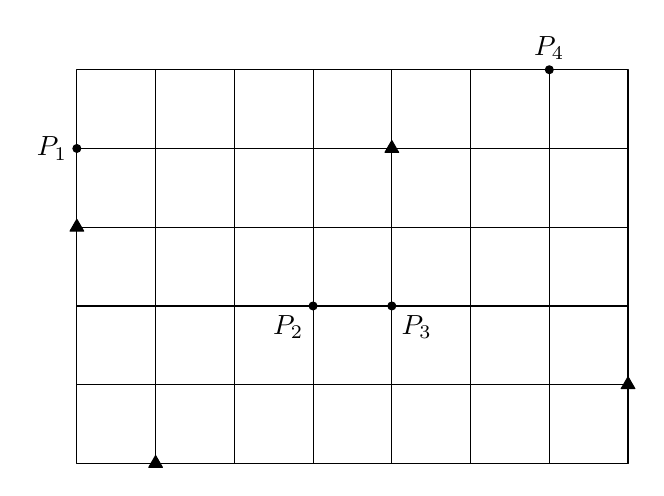
\begin{tikzpicture}[>=latex, line cap = round, line join = round]
    \foreach \i in {0,1,...,7}
        \draw (\i,0) -- (\i,5);
    \foreach \i in {0,1,...,5}
        \draw (0,\i) -- (7,\i);
    \filldraw (0,4) circle (0.05) node [left] {$P_1$};
    \filldraw (3,2) circle (0.05) node [below left] {$P_2$};
    \filldraw (4,2) circle (0.05) node [below right] {$P_3$};
    \filldraw (6,5) circle (0.05) node [above] {$P_4$};
    \filldraw (1,0) ++ (210:0.1) --++ ({0.1*sqrt(3)},0) --++ (120:{0.1*sqrt(3)}) -- cycle;
    \filldraw (0,3) ++ (210:0.1) --++ ({0.1*sqrt(3)},0) --++ (120:{0.1*sqrt(3)}) -- cycle;
    \filldraw (4,4) ++ (210:0.1) --++ ({0.1*sqrt(3)},0) --++ (120:{0.1*sqrt(3)}) -- cycle;
    \filldraw (7,1) ++ (210:0.1) --++ ({0.1*sqrt(3)},0) --++ (120:{0.1*sqrt(3)}) -- cycle;
\end{tikzpicture}
\end{center}
\item (003381)已知三点$A(2,-3)$、$B(-2,-5)$, 求分别满足下列条件的圆方程:\\
(1) 以$A$、$B$两点为直径的圆为\blank{50};\\
(2) 过$A$、$B$两点, 且圆心在直线$x-2y-3=0$上的圆为\blank{50}.
\item (003382)若方程$x^2+y^2+ax+2ay+2a^2+a-1=0$表示圆, 则$a$的取值范围是\blank{50}.
\item (003383)(1) 过点$(3,4)$作圆$x^2+y^2=25$的切线$l$, 则$l$的方程为\blank{50};\\
(2) 过点$(2,4)$作圆$x^2+y^2-2x=0$的切线$m$, 则$m$的方程为\blank{50}.
\item (003384)若点$P$在圆$x^2+y^2+4x-6y+12=0$上运动, 点$Q$在直线$4x+3y=21$上运动, 则$|PQ|$的最小值是\blank{50}.
\item (003385)已知圆$x^2+y^2=8$内一点$P(-1,2)$, 过点$P$作直线$l$交圆于$A$、$B$, 若弦$AB$恰被点$P$平分, 则直线$l$的方程为\blank{50}.
\item (003386)若直线$ax+by=1$与圆$C:x^2+y^2=1$相交, 则点$P(a,b)$与圆$C$的位置关系是\bracket{20}.
\twoch{点在圆内}{点在圆上}{点在圆外}{随$a,b$取值的变化而变化}
\item (003387)若关于$x$的方程$x+\sqrt{4-x^2}=m$有且仅有一个实数解, 则实数$m$的取值范围是\blank{50}.
\item (003388)设$f(x,y)=ax+by+c$, 其中$a,b$不全为零. 给定直线$l:f(x,y)=0$及其外一点$P(x_0,y_0)$, 直线$m:f(x,y)-f(x_0,y_0)=0$, 则\bracket{20}
\twoch{点$P$在直线$m$上, 直线$m$与$l$平行}{点$P$在直线$m$上, 直线$m$与$l$不平行}{点$P$在直线$m$外, 直线$m$与$l$平行}{点$P$在直线$m$外, 直线$m$与$l$不平行}
\item (003389)已知圆$C:x^2+y^2-4x-14y+45=0$及点$Q(-2,3)$.\\
(1) 若$P(m,m+1)$在圆$C$上, 求线段$PQ$的长及直线$PQ$的斜率;\\
(2) 若$P$为圆$C$上任意一点, 求线段$PQ$的长的最大值和最小值;\\
(3) 若点$M(a,b)$在圆$C$上, 求$u=\dfrac{b-3}{a+2}$的最大值和最小值.
\item (003390)过原点的直线与圆$x^2+y^2-6x+5=0$相交于$A$、$B$两点, 求弦$AB$的中点$M$的轨迹方程.
\item (003391)已知圆$C:x^2+y^2=25$, 过定点$P(-4,0)$的直线$l$交圆$C$于$A$、$B$两点.\\
(1) 若直线$l$的斜率为$1$, 求弦长$|AB|$;\\
(2) 求弦长$|AB|$的取值范围;\\
(3) 求$\triangle AOB$面积的取值范围.
\item (003392)圆$x^2+y^2-2x-4y-1=0$关于直线$x-y+3=0$的对称的曲线的方程为\blank{50}.
\item (003393)若直线$mx+ny-3=0$与圆$x^2+y^2=3$没有公共点, 则$m^2+n^2$的取值范围为\blank{50}.
\item (003394)方程$|x|-1=\sqrt{1-y^2}$表示的曲线是\bracket{20}.
\twoch{一条直线}{两条射线}{一个圆}{两个半圆(即两段圆弧)}
\item (003395)求满足下列条件的圆的方程:\\
(1) 经过点$(2,-1)$且和直线$x-y=1$相切, 同时圆心在直线$y=-2x$上的圆的方程为\blank{50};\\
(2) 经过点$A(-2,-4)$, 且与直线$l:x+3y-26=0$相切于点$B(8,6)$的圆的方程为\blank{50}.
\item (003396)已知方程$x^2+y^2+Dx+Ey+F=0$表示一个圆. ``$D^2=4F$''是``该圆与$x$轴相切''的\bracket{20}条件.
\fourch{充分非必要}{必要非充分}{充要}{既非充分又非必要}
\item (003397)圆$x^2+y^2=4$与$x$轴相交于$A$、$B$两点, 圆内的动点$P$使$|PA|$, $|PO|$, $|PB|$成等比数列, 求$\overrightarrow{PA}\cdot \overrightarrow{PB}$的取值范围.
\item (003398)已知$m\in \mathbf{R}$, 直线$l:mx-(m^2+1)y=4m$和圆$C:x^2+y^2-8x+4y+16=0$.\\
(1) 求直线$l$的斜率$k$的取值范围;\\
(2) 直线$l$能否将圆$C$分割成弧长的比值为$\dfrac{1}{2}$的两段圆弧? 为什么?
\item (003399)若点$P(-3,0)$是椭圆$x^2+2y^2-k=0$上的点, 则椭圆的焦点坐标是\blank{50}.
\item (003400)方程$\dfrac{x^2}{k-5}+\dfrac{y^2}{3-k}=-1$表示焦点在$y$轴上的椭圆, 则实数$k$的取值范围是\blank{50}.
\item (003401)(1) 焦距是$2\sqrt 5$, 长轴长是$8$的椭圆的标准方程是\blank{50};\\
(2) 长轴长是短轴长的2倍, 且经过点$(2,1)$的椭圆的标准方程是\blank{50};\\
(3) 经过点$A(\sqrt 3,-2)$、$B(\sqrt 5,\dfrac{\sqrt{30}}3)$的椭圆的方程是\blank{50}.
\item (003402)已知点$P$是椭圆$\dfrac{x^2}{25}+\dfrac{y^2}9=1$上一点, $F_1F_2$是焦点, 若$\angle F_1PF_2=60^\circ$, 则三角形$F_1PF_2$的面积为\blank{50}.
\item (003403)已知椭圆$\dfrac{x^2}{36}+\dfrac{y^2}{16}$=1的弦过点$P(3,2)$且被$P$平分, 则此弦所在的直线方程为\blank{50}.
\item (003404)椭圆$\dfrac{x^2}{45}+\dfrac{y^2}{20}=1$的焦点为$F_1$、$F_2$, 过原点$O$作直线交椭圆于$A$、$B$两点, 若$\triangle ABF_2$的面积为$20$, 则点$A$的纵坐标为\blank{50}.
\item (003405)若曲线$\dfrac{x^2}2+y^2=1 \ (y\ge 0)$与$y=x+m$有两个公共点, 则实数$m$的取值范围为\blank{50}.
\item (003406)已知椭圆$\dfrac{x^2}m+\dfrac{y^2}6=1$, $F_1,F_2$是它的两个焦点, 若椭圆上存在两个不同的点$P$, 使$\angle F_1PF_2=90^\circ$, 则$m=$\blank{50}.
\item (003407)已知椭圆$\dfrac{y^2}9+{x^2}=1$, 一条不与坐标轴平行的直线$l$与该椭圆交于不同的两点$M$、$N$, 且线段$MN$的中点的横坐标为$-\dfrac 12$.\\
(1) 求直线$l$的斜率的取值范围;\\
(2) 求直线$l$的倾斜角的取值范围.
\item (003408)已知椭圆$\dfrac{x^2}2+{y^2}=1$.\\
(1) *过椭圆的左焦点$F$引椭圆的割线, 求截得的弦的中点$P$的轨迹方程;\\
(2) 求斜率为2的平行弦中点$Q$的轨迹方程;\\
(3) 求过点$M(\dfrac 12,\dfrac 12)$且被$M$平分的弦所在直线方程.
\item (003409)设椭圆$C:\dfrac{x^2}2+{y^2}=1$的右焦点为$F$, 过$F$的直线$l$与$C$交于$AB$两点, 点$M$的坐标为$(2,0)$.\\
(1) 当$l$与$x$轴垂直时, 求直线$AM$的方程;\\
(2) 设$O$为坐标原点, 证明: $\angle OMA=\angle OMB$.
\item (003410)若椭圆的中心为原点, 焦点在坐标轴上, 焦点到长轴端点的距离分别为$\sqrt 2-1$与$\sqrt 2+1$, 则椭圆的方程为\blank{50}.
\item (003411)与椭圆$\dfrac{x^2}9+\dfrac{y^2}4=1$有相同的焦点, 且经过点$(3,-2)$的椭圆为\blank{50}.
\item (003412)已知圆$A:(x-4)^2+y^2=100$, 圆$B:(x+4)^2+y^2=1$, 动圆P与圆$A$内切且与圆$B$外切, 则点P的轨迹方程是\blank{50}.
\item (003413)椭圆${x^2}+\dfrac{y^2}4=1$上的点$P(x,y)$到定直线$x+y-6=0$的最远距离是\blank{50}.
\item (003414)记椭圆$\dfrac{x^2}4+\dfrac{n{y^2}}{4n+1}=1$围成的区域(含边界)为$\Omega_n \ (n=1,2,\cdots)$, 当点$(x,y)$分别在$\Omega_1,\Omega_2,\cdots$上时, $x+y$的最大值分别是$M_1,M_2,\cdots$, 则$\displaystyle\lim_{n\to \infty}M_n=$\blank{50}.
\item (003415)椭圆$\dfrac{x^2}9+\dfrac{y^2}4=1$上的动点$P(x,y)$与定点$M(m,0)$($0<m<3$)的距离的最小值为$1$, 求$m$的值.
\item (003416)在平面直角坐标系$xOy$中, 经过点$(0,\sqrt 2)$且斜率为$k$的直线$l$与椭圆$\dfrac{x^2}2+y^2=1$有两个不同的交点$P$、$Q$.\\
(1) 求$k$的取值范围;\\
(2) 设椭圆与$x$轴正半轴、$y$轴正半轴的交点分别为$A$、$B$. 问是否存在常数$k$, 使得向量$\overrightarrow{OP}+\overrightarrow{OQ}$与$\overrightarrow{AB}$共线? 如果存在, 求出$k$的值; 如果不存在, 说明理由.
\item (003417)*在平面直角坐标系$xOy$中, 已知椭圆$\Gamma:\dfrac{x^2}4+{y^2}=1$, $A$为$\Gamma$的上顶点, $P$为$\Gamma$上异于上、下顶点的动点, $M$为正半轴上的动点.\\
(1) 若$P$在第一象限, 且$|OP|=\sqrt 2$, 求$P$的坐标;\\
(2) 设$P(\dfrac 85,\dfrac 35)$, 若以$A$、$P$、$M$为顶点的三角形是直角三角形, 求$M$的横坐标$m$;\\
(3) 若$|MA|=|MP|$, 直线$AQ$与$\Gamma$交于另一点$C$, 且$\overrightarrow{AQ}=2\overrightarrow{AC}$, $\overrightarrow{PQ}=4\overrightarrow{PM}$, 求直线$AQ$的方程.
\item (003418)已知双曲线的中心在原点, 焦点在坐标轴上. 分别求满足下列条件的双曲线的标准方程:\\
(1) 以椭圆$\dfrac{x^2}{25}+\dfrac{y^2}9=1$的长轴顶点为焦点, 且过$P(4\sqrt 2,3)$的双曲线方程为\blank{50};\\
(2) 点$P(\sqrt 2,1)$在双曲线上, 且它到双曲线的右焦点的距离是$1$, 该双曲线方程为\blank{50}.
\item (003419)双曲线顶点间距离为$6$, 渐近线方程为$y=\pm \dfrac 32x$, 该双曲线方程为\blank{50}.
\item (003420)双曲线$4x^2+ky^2-4k=0$的虚轴长为\blank{50}.
\item (003421)双曲线$\dfrac{x^2}4-\dfrac{y^2}8=1$的两条渐近线所夹的锐角的大小为\blank{50}.
\item (003422)已知$F_1$、$F_2$是双曲线$\dfrac{x^2}{16}-\dfrac{y^2}{20}=1$的焦点, 点$P$在双曲线上. 若$|PF_1|=9$, 则$|PF_2|=$\blank{50}.
\item (003423)直线$y=kx+2$与双曲线$x^2-y^2=6$的右支交于不同的两点, 则$k$的取值范围为\blank{50}.
\item (003424)已知动圆$M$与圆$C_1:(x+4)^2+y^2=2$, 与圆$C_2:(x-4)^2+y^2=2$相内切, 则动圆圆心$M$的轨迹方程为\blank{50}.
\item (003425)已知两点$M(-5,0)$, $N(5,0)$. 在下列直线上, 存在点$P$满足$|MP|-|NP|=6$的所有直线方程是\blank{50}(填写序号).\\ \textcircled{1} $y=\dfrac 53(x+2)$; \textcircled{2} $y=\dfrac 53(x-5)$; \textcircled{3} $y=x-2$; \textcircled{4} $y=4(x+2)$.
\item (003426)已知双曲线$C$的一个顶点$A(0,\sqrt 2)$, 其渐近线经过原点且与圆$M:(x-\sqrt 2)^2+y^2=1$相切.\\
(1) 求双曲线$C$的方程;\\
(2) 已知直线$l:y=x-\sqrt 2$, 在双曲线的上支求点$P$, 使点$P$与直线$l$的距离等于$\sqrt 2$.
\item (003427)在双曲线$\dfrac{y^2}{12}-\dfrac{x^2}{13}=1$上支上有不同三点$A(x_1,y_1)$、$B(\sqrt{26},6)$、$C(x_2,y_2)$到焦点$F(0,5)$的距离成等差数列.\\
(1) 求$y_1+y_2$的值;\\
(2) 证明: 线段$AC$的垂直平分线经过一个定点$T$并且求出这个点$T$的坐标.
\item (003428)若椭圆$\dfrac{x^2}{m^2}+\dfrac{y^2}{n^2}=1$($m>n>0$)和双曲线$\dfrac{x^2}{a^2}-\dfrac{y^2}{b^2}=1$($a>0$, $b>0$)有相同的焦点$F_1,F_2$, 点$P$是椭圆和双曲线的一个交点.\\
(1) 求证: $|PF_1|\cdot |PF_2|=m^2-a^2$;\\
(2) 求证: $\triangle PF_1F_2$的面积$S=nb$.
\item (003429)若双曲线$8mx^2-my^2=8$的一个焦点是$(0,3)$, 则$m=$\blank{50};
\item (003430)和双曲线$\dfrac{x^2}9-\dfrac{y^2}{16}=1$有共同的渐近线, 并且实轴长为$12$的双曲线方程是\blank{50};
\item (003431)过$P(1,0)$作直线$l$与双曲线${x^2}-\dfrac{y^2}4=1$只有一个公共点, 则这样的直线共有\blank{50}条.
\item (003432)已知双曲线$\dfrac{x^2}{12}-\dfrac{y^2}4=1$的右焦点为$F$, 若过点$F$的直线$l$与双曲线的右支有且只有一个公共点, 则直线$l$的斜率的取值范围为\blank{50}.
\item (003433)若关于$x$的方程$\sqrt{x^2-1}=x+m$没有实数解, 则实数$m$的取值范围是\blank{50};
\item (003434)求渐近线为$3x\pm 4y=0$, 焦点为椭圆$\dfrac{x^2}{10}+\dfrac{y^2}5=1$的一对顶点的双曲线方程.
\item (003435)已知$F_1F_2$是双曲线${x^2}-\dfrac{y^2}{b^2}=1$($b>0$)的左、右焦点, 直线$l$过$F_2$且与双曲线交于$AB$两点.\\
(1) 若$l$的倾斜角为$\dfrac{\pi}2$, $\triangle F_1AB$是等边三角形, 求双曲线的渐近线方程;\\
(2) 设$b=\sqrt 3$, 若$l$的斜率存在, 且$(\overrightarrow{F_1A}+\overrightarrow{F_1B})\cdot \overrightarrow{AB}=0$, 求$l$的斜率.
\item (003436)设双曲线${x^2}-\dfrac{y^2}4=1$的右顶点为$A$, 定点$B$的坐标为$(\dfrac 12,1)$.\\
(1) 是否存在过$B(\dfrac 12,1)$点且被点$B$平分的双曲线的弦$PQ$, 若存在求出弦$PQ$所在直线方程, 若不存在说明理由;\\
(2) 过点$B$的动直线$l$交双曲线于$P,Q$两点, $M$为线段$PQ$的中点, 求直线$AM$的斜率的取值范围.
\item (003437)已知抛物线的顶点在原点, 焦点在坐标轴上. 分别求适合下列条件的抛物线的标准方程:\\
(1) 过点$(-2,3)$的抛物线为\blank{50};\\
(2) 准线过点$(2,3)$的抛物线为\blank{50};\\
(3) 焦点在直线$3x-4y-12=0$上的抛物线为\blank{50};\\
(4) 焦点在$y$轴上, 抛物线上一点$M(m,-3)$到焦点的距离等于$5$的抛物线为\blank{50}.
\item (003438)过点$(2,1)$与抛物线$y=x^2$恰有一个公共点的直线有\blank{50}条.
\item (003439)抛物线$y=x^2$上到直线$2x-y=4$距离最短的点的坐标为\blank{50}.
\item (003440)已知点$A(3,4)$, $F$是抛物线$y^2=8x$的焦点, $M$是抛物线上的动点.当$|MA|+|MF|$最小时, $M$的坐标是\blank{50}.
\item (003441)若$AB$是抛物线$y=x^2$的一条过焦点的弦, 且$|AB|=4$, 则$AB$的中点到直线$y+1=0$的距离是\blank{50}.
\item (003442)一动点到定点$A(0,2)$的距离比定直线$y=-3$的距离小$1$, 则动点的轨迹方程是\blank{50}.
\item (003443)已知$F$是抛物线$C:y^2=4x$的焦点, $AB$是抛物线$C$上的两个点, 线段$AB$的中点为$M(2,2)$, 则$\triangle ABF$的面积等于\blank{50}.
\item (003444)已知$A,B$是抛物线$y^2=2px(p>0)$上的两个点, $O$为坐标原点, 若$|OA|=|OB|$, 且抛物线的焦点恰为$\triangle AOB$的垂心, 则直线$AB$的方程是\blank{50}.
\item (003445)已知点$M$到点$F(1,0)$和直线$x=3$的距离之和等于$4$, 设点$M$的轨迹为曲线$\Gamma$.\\
(1) 求曲线$\Gamma$的方程;\\
(2) 过点$F$作倾斜角为$\dfrac{\pi}4$的直线交曲线$\Gamma$于$A$、$B$两点, 求$|AB|$的值.
\item (003446)如图, $M$是抛物线上$y^2=x$上的一点(异于原点), 动弦$ME$、$MF$分别交$x$轴于$AB$两点, 且$MA=MB$.\\
(1) 若$M$为定点, 证明: 直线$EF$的斜率为定值;\\
(2) 若$M$为动点, 且$\angle EMF={90}^{\circ}$, 求$\triangle EMF$的重心$G$的轨迹.
\begin{center}
\begin{tikzpicture}[>=latex, line cap = round, line join = round, scale = 1.5]
    \draw [->] (-0.5,0) -- (4,0) node [below] {$x$};
    \draw [->] (0,-2) -- (0,2) node [left] {$y$};
    \draw (0,0) node [below left] {$O$};    
    \draw [domain = -1.8:1.8, samples = 1000] plot (\x*\x, \x);
    \draw (1.44,1.2) node [above] {$M$};
    \draw (0.49,-0.7) node [below] {$E$} -- (1.44,1.2) -- (2.89,-1.7) node [below] {$F$} -- cycle;
    \draw (0.84,0) node [below right] {$A$} (2.04,0) node [above right] {$B$};
\end{tikzpicture}
\end{center}
\item (003447)求证: 抛物线的准线上任意一点引抛物线的两切线互相垂直并且切点弦过定点.
\item (003448)抛物线$y=-4x^2$的焦点坐标是\blank{50}.
\item (003449)抛物线的焦点在双曲线$\dfrac{x^2}{25}-\dfrac{y^2}4=1$上, 则抛物线的标准方程\blank{50}.
3.点$A(-4,2)$是抛物线$y^2=-8x$内一点, 抛物线上的点$M$到$A$点的距离与它到焦点的距离之和最小, 则点$M$的坐标是\blank{50}, 最小距离是\blank{50}.
4.设$F$为抛物线$y^2=4x$的焦点, $ABC$为该抛物线上三点.若$\overrightarrow{FA}+\overrightarrow{FB}+\overrightarrow{FC}=\overrightarrow 0$, 则$|\overrightarrow{FA}|+|\overrightarrow{FB}|+|\overrightarrow{FC}|=$\blank{50}.
5.设抛物线$y^2=2x$的焦点为$F$, 过点$M(\sqrt 3,0)$的直线与抛物线相交于$AB$两点, 与抛物线的准线相交于$C$, $| BF |=2$, 则$\triangle BCF$与$\triangle ACF$的面积之比为\blank{50}.
\item (003450)设直线$a$与抛物线$\Omega:y^2=4x$相交于不同的两点$AB$, $O$为坐标原点.\\
(1) 求抛物线$\Omega$的焦点到准线的距离;\\
(2) 若$\overrightarrow{OA}\cdot \overrightarrow{OB}=0$, 点$Q$在线段$AB$上, 满足$OQ\perp AB$, 求点$Q$的轨迹.
\item (003451)如图, 已知点$P$是$y$轴左侧(不含$y$轴)一点, 抛物线$C:y^2=4x$上存在不同的两点$A$、$B$满足$PA$、$PB$的中点均在$C$上.\\
(1) 设$AB$中点为$M$, 证明: $PM\perp y$轴;\\
(2) 若$P$是半椭圆${x^2}+\dfrac{y^2}4=1x<0$上的动点, 求$\triangle PAB$面积的取值范围.
\begin{center}
\begin{tikzpicture}[>=latex, line cap = round, line join = round, scale = 0.7]
    \draw [->] (-1.5,0) -- (5,0) node [below] {$x$};
    \draw [->] (0,-5) -- (0,5) node [left] {$y$};
    \draw (0,0) node [below right] {$O$};    
    \draw [domain = -4.5:4.5, samples = 1000] plot (\x*\x/4, \x);
    \draw ({11/4+sqrt(10)/2},{1+sqrt(10)}) node [above] {$A$} coordinate (A);
    \draw ({11/4-sqrt(10)/2},{1-sqrt(10)}) node [below] {$B$} coordinate (B);
    \draw ($(A)!0.5!0:(B)$) node [right] {$M$} coordinate (M);
    \draw (-1,1) node [left] {$P$} coordinate (P);
    \draw (P) -- (M) (A) -- (P) -- (B) -- cycle;
\end{tikzpicture}
\end{center}
\item (003452)下列命题中, 假命题有\blank{50}(填入序号).\\
(1) 平行于同一平面的两直线平行; (2) 平行于同一直线的两平面平行; (3) 平行于同一直线的两直线平行; (4) 平行于同一平面的两平面平行.
\item (003453)给定空间中的直线$l$及平面$\alpha$. ``直线$l$与平面$\alpha$内无数条直线都垂直''是``直线$l$与平面$\alpha$垂直''的\blank{50}条件.
\item (003454)对于空间三条直线$a,b,c$, 若$a\perp b$, $b\perp c$, 则$a$与$c$\bracket{20}.
\twoch{一定相交}{一定平行}{一定异面}{平行、相交、异面都有可能}
\item (003455)如图是一个正方体的展开图. 在原正方体中, 直线$AB$与$CD$所成的角的大小为\blank{50}.
\begin{center}
    \begin{tikzpicture}[>=latex, line cap = round, line join = round, scale = 1.5]
        \draw (0,0) -- (3,0) (0,1) node [above left] {$A$} -- (4,1) (1,-1) -- (2,-1) (2,2) node [above left] {$C$} -- (4,2);
        \draw (0,0) -- (0,1) (1,-1) -- (1,1) (2,-1) -- (2,2) (3,0) -- (3,2) (4,1) -- (4,2);
        \draw (0,1) -- (1,0) node [below right] {$B$} coordinate (B) (2,2) -- (3,1) node [below right] {$D$};
        \draw [dashed] (B) --++ (45:1/2) --++ (1,0) --++ (225:1/2);
        \draw [dashed] (B) ++ (0,1) --++ (45:1/2) --++ (1,0) --++ (225:1/2);
        \draw [dashed] (B) ++ (45:1/2) --++ (0,1) ++ (1,0) --++ (0,-1);
    \end{tikzpicture}
\end{center}
\item (003456)直线$PA$垂直于矩形$ABCD$所在的平面. 设$AP=AD=1$, $DC=2$, 则点$P$到直线$BD$的距离为\blank{50}.
\item (003457)空间四边形$ABCD$中, 点$E,F,G$分别是边$AB,BC,CD$的中点. 若异面直线$AC$与$BD$所成的角的大小为$60^\circ$, 则$\angle EFG$的大小为\blank{50}.
\item (003458)已知$P$是二面角$\alpha-l-\beta$内一点, 过$P$作$PA\perp \alpha$, $PB\perp \beta$, $A,B$为垂足, 若直线$PA$与$PB$所成角的大小是$80^\circ$, 则二面角$\alpha-l-\beta$的大小是\blank{50}.
\item (003459)由一点$P$出发引三条射线$PA$, $PB$, $PC$, 若$\angle APB=45^\circ$, $\angle APC=60^\circ$, $\angle BPC=90^\circ$, 则$PA$与平面$BPC$所成角的大小是\blank{50}.
\item (003460)如图, 在长方体$ABCD-A_1B_1C_1D_1$中, 点$E,F$分别在棱$BB_1, DD_1$上, 且$AE\perp A_1B$, $AF\perp A_1D$. 求证: $A_1C\perp$平面$AEF$.
\begin{center}
    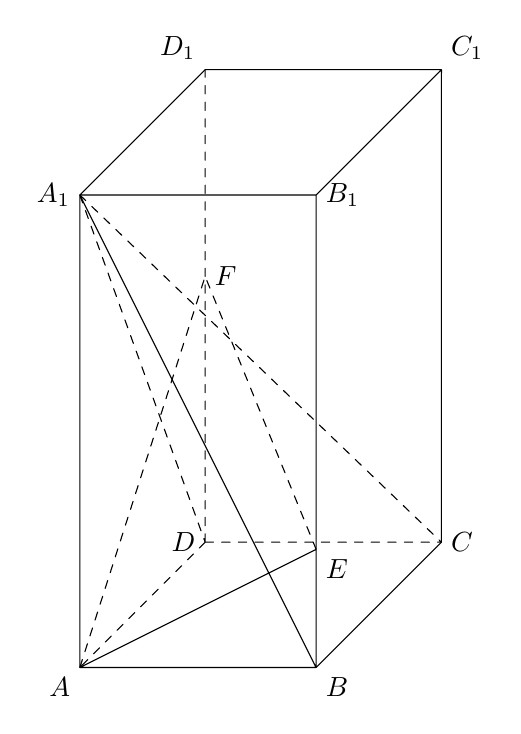
\begin{tikzpicture}[>=latex, line cap = round, line join = round, scale = 1.5]
        \draw (0,0) coordinate (A) node [below left] {$A$};
        \draw (A) ++ (2,0) coordinate (B) node [below right] {$B$};
        \draw (A) ++ (45:1.5) coordinate (D) node [left] {$D$};
        \draw (D) ++ (2,0) coordinate (C) node [right] {$C$};
        \draw (B) ++ (0,1) coordinate (E) node [below right] {$E$};
        \draw (D) ++ (0,9/4) coordinate (F) node [right] {$F$};
        \draw (A) ++ (0,4) coordinate (A1) node [left] {$A_1$};
        \draw (B) ++ (0,4) coordinate (B1) node [right] {$B_1$};
        \draw (C) ++ (0,4) coordinate (C1) node [above right] {$C_1$};
        \draw (D) ++ (0,4) coordinate (D1) node [above left] {$D_1$};
        \draw (A) -- (B) -- (C) -- (C1) -- (D1) -- (A1) -- cycle (C1) -- (B1) -- (B) (B1) -- (A1) (A1) -- (B) (A) -- (E);
        \draw [dashed] (D) -- (A) (D) -- (C) (D) -- (D1) (A1) -- (C) (A) -- (F) -- (E) (A1) -- (D);
    \end{tikzpicture}
\end{center}
\item (003461)如图, 在棱长为$2$的正方体$ABCD-A_1B_1C_1D_1$中, $E$是$BC_1$的中点.
\begin{center}
\begin{tikzpicture}[>=latex, line cap = round, line join = round]
    \draw (0,0) node [below left] {$A$} coordinate (A) -- (4,0) node [below right] {$B$} coordinate (B) --++ (45:{4/2}) node [right] {$C$} coordinate (C)
    --++ (0,4) node [above right] {$C_1$} coordinate (C1)
    --++ (-4,0) node [above left] {$D_1$} coordinate (D1) --++ (225:{4/2}) node [left] {$A_1$} coordinate (A1) -- cycle;
    \draw (4,4) node [right] {$B_1$} coordinate (B1) -- (B) (B1) --++ (45:{4/2}) (B1) --++ (-4,0);
    \draw [dashed] (0,0) --++ (45:{4/2}) node [left] {$D$} coordinate (D) --++ (4,0) (D) --++ (0,4);
    \draw (C1) -- (B);
    \draw ($(B)!0.5!0:(C1)$) node [right] {$E$} coordinate (E);
    \draw [dashed] (E) -- (D);
    \filldraw ($(A)!0.5!0:(B)$) node [below] {$P$} circle (0.02);
    \filldraw ($(A)!0.5!0:(D)$) node [left] {$Q$} circle (0.02);
    \filldraw ($(B1)!0.5!0:(C1)$) node [above] {$R$} circle (0.02);
\end{tikzpicture}
\end{center}
(1) 求直线$DE$与平面$ABCD$所成的角的大小;\\
(2) 在图中作出过点$D_1,D,E$三点的正方体$ABCD-A_1B_1C_1D_1$的截面, 并求出该截面的面积;\\
(3) $P,Q,R$分别是$AB,AD,B_1C_1$的中点, 作出过$P,Q,R$的截面.
\item (003462)如图, $P$为三角形$ABC$所在平面外一点, $PA\perp$平面$ABC$, $\angle ABC=90^\circ$, $AE\perp PB$于$E$, $AF\perp PC$于$F$.
\begin{center}
\begin{tikzpicture}[>=latex, line cap = round, line join = round]
    \draw (0,0) coordinate (B) (3,0) coordinate (C) (1,1) coordinate (A) node [below] {$A$} (1,4) coordinate (P);
    \draw (B) node [below left] {$B$} -- (C) node [below right] {$C$} -- (P) node [above] {$P$} -- cycle;
    \draw ($(B)!0.6!0:(P)$) coordinate (E) node [left] {$E$} ($(C)!0.65!0:(P)$) coordinate (F) node [right] {$F$};
    \draw (E) -- (F);
    \draw [dashed] (A) -- (P) (A) -- (B) (A) -- (C) (A) -- (E) (A) -- (F); 
\end{tikzpicture}
\end{center}
(1) 求证: $BC\perp$平面$PAB$, $AE\perp$平面$PBC$, $PC\perp$平面$AEF$;\\
(2) 若$AP=AC=2$, $\angle BPC=\theta$, 当$\theta$为何值时, 三角形$AEF$的面积$S$取到最大值? 最大值是多少?
\item (003463)空间中有四个点, ``这四个点中恰好有三点在同一直线上''是``这四个点在同一个平面上''的\blank{50}条件;
\item (003464)两条直线$a$、$b$满足$a\parallel b$, $b\subsetneqq \alpha$, 则$a$与平面$\alpha$的关系是\blank{50}.
\item (003465)对于平面$M$、$N$. ``$M$内有不共线的三点到$N$的距离相等''是``$M\parallel N$''成立的\blank{50}条件;
\item (003466)对于分别与两条异面直线都相交的两条直线, 下列结论中, 真命题有\blank{50}(填入序号).\\
(1) 一定是异面直线; (2) 不可能是平行直线; (3) 不可能是相交直线.
\item (003467)已知$A,B$两点到平面$\alpha$的距离分别是$1$和$3$, 那么线段$AB$的中点到平面$\alpha$的距离是\blank{50}.
\item (003468)如图, 点$P$为三棱柱$ABC-A_1B_1C_1$的侧棱$BB_1$上一点, $PM\perp BB_1$交$AA_1$于点$M$, $PN\perp BB_1$交$CC_1$于点$N$. 求证: $CC_1\perp MN$.
\begin{center}
\begin{tikzpicture}[>=latex, line cap = round, line join = round, scale = 1.4]
    \draw (0,0) node [below left] {$B_1$} coordinate (B1) -- (2,0) node [below right] {$C_1$} coordinate (C1) 
    -- ++ (0.5,3) node [right] {$C$} coordinate (C) --++ (-2,0) node [left] {$B$} coordinate (B) -- cycle;
    \draw (B) --++ (1.7,0.5) node [above] {$A$} coordinate (A) -- (C);
    \draw [dashed] (A) --++ (-0.5,-3) node [above left] {$A_1$} coordinate (A1) -- (C1) (A1) -- (B1);
    \draw ($(B)!0.5!0:(B1)$) node [left] {$P$} coordinate (P);
    \draw ($(C)!0.6!0:(C1)$) node [right] {$N$} coordinate (N);
    \draw ($(A)!0.55!0:(A1)$)node [above left] {$M$} coordinate (M);
    \draw (P) -- (N);
    \draw [dashed] (N) -- (M) -- (P);
\end{tikzpicture}
\end{center}
\item (003469)如图, 在长方体$ABCD-A'B'C'D'$中, $AB=2$, $AD=1$, $AA'=1$. 证明:\\
(1) 直线$BC'$与直线$AC$异面;\\
(2) 直线$BC'\parallel\text{平面}ACD'$, 并求$BC'$到平面$ACD'$的距离.
\begin{center}
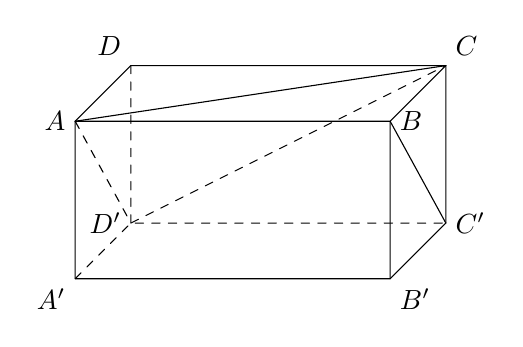
\begin{tikzpicture}[>=latex, line cap = round, line join = round, scale = 2]
    \draw (0,0) node [below left] {$A'$} coordinate (AP) --++ (2,0) node [below right] {$B'$} coordinate (BP) --++ (45:{1/2}) node [right] {$C'$} coordinate (CP)
    --++ (0,1) node [above right] {$C$} coordinate (C)
    --++ (-2,0) node [above left] {$D$} coordinate (D) --++ (225:{1/2}) node [left] {$A$} coordinate (A) -- cycle;
    \draw (AP) ++ (2,1) node [right] {$B$} coordinate (B) -- (BP) (B) --++ (45:{1/2}) (B) --++ (-2,0);
    \draw [dashed] (AP) --++ (45:{1/2}) node [left] {$D'$} coordinate (DP) --++ (2,0) (DP) --++ (0,1);
    \draw (B) -- (CP) (A) -- (C);
    \draw [dashed] (A) -- (DP) -- (C);
\end{tikzpicture}
\end{center}
\item (003470)下列命题中, 假命题有\blank{50}(填入序号).\\
(1) 底面是正多边形的棱锥是正棱锥; (2) 侧棱都相等的棱锥是正棱锥; (3) 有两个侧面是矩形的棱柱是直棱柱.
\item (003471)正四棱锥底面边长为$4$, 侧棱长为$3$, 则其侧面积为\blank{50}, 其体积为\blank{50}.
\item (003472)棱锥的高是$1$, 一个平行于底面的平面把棱锥分成体积相等的两个部分, 则顶点到这个平行于底面的平面的距离为\blank{50}.
\item (003473)棱长为$1$的正四面体的高为\blank{50}, 体积为\blank{50}, 对棱中点的距离为\blank{50}.
\item (003474)若两个长方体的长, 宽, 高分别为$5$, $4$, $3$, 把它们两个全等的面重合在一起组成大长方体, 则大长方体的对角线最长为\blank{50}.
\item (003475)若一个圆柱的侧面展开图是一个正方形, 则这个圆柱的表面积与侧面积的比是\blank{50}.
\item (003476)若圆锥的侧面展开图恰好是一个半圆, 则该圆锥的母线与底面所成的角的大小是\blank{50}.
\item (003477)过半径为$2$的球$O$表面上一点$A$作球$O$的截面, 若$OA$与该截面所成的角的大小为$60^\circ$, 则该截面的面积是\blank{50}.
\item (003478)如图, 圆锥的轴截面为等边三角形$SAB$, $Q$为底面圆周上一点.
\begin{center}
\begin{tikzpicture}[>=latex, line cap = round, line join = round, scale = 1]
    \draw (-3,0) node [left] {$A$} arc (180:360:3 and 1) node [right] {$B$} -- (0,6) coordinate (S) node [above] {$S$} -- cycle;
    \draw [dashed] (-3,0)  arc (180:0:3 and 1);
    \draw ({-3*cos(40)},{-sin(40)}) node [below left] {$Q$} coordinate (Q) -- (0,6);
    \draw [dashed] (Q) -- (3,0) coordinate (B);
    \draw [dashed] ($(Q)!0.5!0:(B)$) node [below] {$C$} coordinate (C) -- (S) -- (0,0) node [above left] {$O$} coordinate (O);
    \draw [dashed] (O) -- ($(C)!0.08!0:(S)$) node [right] {$M$} (B) -- (-3,0);
\end{tikzpicture}
\end{center}
(1) 设$C$为线段$BQ$的中点, $M$是$SC$上一点, 且$OM\perp SC$, 证明: $OM\perp\text{平面}SBQ$;\\
(2) 若$\angle AOQ=60^\circ$, $QB=2\sqrt 3$, 求圆锥的体积.
\item (003479)取地球的半径为$6370$千米, 在北纬$45^\circ$线上, 求相隔$30^\circ$的两条经线之间的球面距离(精确到$0.1$千米).
\item (003480)直三棱柱$ABC-A_1B_1C_1$中, 底面$ABC$为等腰直角三角形, 且$AB\perp AC$, $AB=AC=2$, $AA_1=4$, $M$是侧棱$CC_1$上一点, 设$MC=h$.\\
(1) 若$BM\perp A_1C$, 求$h$的值;\\
(2) 若直线$AM$与平面$ABC$所成的角为$\dfrac{\pi}4$, 求多面体$ABM-A_1B_1C_1$的体积.
\item (003481)过棱锥的高的三等分点作两个平行于底面的截面, 它们将棱锥的侧面分成三部分的面积的比(自顶点开始向底面排序)为\blank{50}.
\item (003482)已知一个凸多面体共有$9$个面, 所有棱长都为$1$, 其平面展开图如图所示, 则该凸多面体的体积为\blank{50}.
\begin{center}
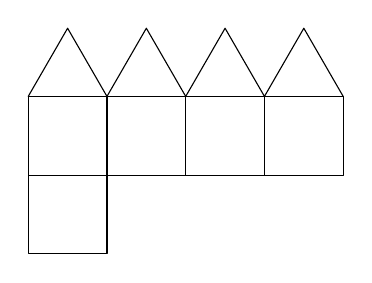
\begin{tikzpicture}[>=latex, line cap = round, line join = round, scale = 1]
    \draw (0,0) -- (4,0) -- (4,1) -- (0,1) -- cycle;
    \draw (0,0) -- (0,-1) -- (1,-1) -- (1,1) (2,1) -- (2,0) (3,1) -- (3,0);
    \draw (0,1) --++ ({1/2},{1/2*sqrt(3)}) --++ ({1/2},{-1/2*sqrt(3)}) --++ ({1/2},{1/2*sqrt(3)}) --++ ({1/2},{-1/2*sqrt(3)}) --++ ({1/2},{1/2*sqrt(3)}) --++ ({1/2},{-1/2*sqrt(3)})
    --++ ({1/2},{1/2*sqrt(3)}) --++ ({1/2},{-1/2*sqrt(3)});
\end{tikzpicture}
\end{center}
\item (003483)若圆锥的侧面积为$20\pi$, 且母线与底面所成的角的大小为$\arccos\dfrac 45$, 则该圆锥的体积为\blank{50}.
\item (003484)下列命题中, 假命题有\blank{50}(填入序号).\\
(1) 经过球上任意两点, 能且仅能作一个大圆;\\
(2) 与球的一条直径垂直的大圆有且只有一个;\\
(3) 球的表面积是它大圆面积的$4$倍;\\
(4) 如果过球面上两点可以作小圆, 那么``小圆的劣弧长''大于``过这两点的大圆的劣弧长''.
\item (003485)圆柱形容器内部盛有高度为$8\text{cm}$的水, 若放入三个相同的球(球的半径与圆柱的底面半径相同)后, 水恰好淹没最上面的球(如图所示), 则球的半径是\blank{50}.
\begin{center}
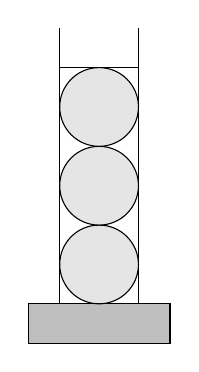
\begin{tikzpicture}
    \draw (0,3.5) -- (0,0) -- (1,0) -- (1,3.5);
    \filldraw [fill = gray!50] (-0.4,0) rectangle (1.4,-0.5);
    \filldraw [fill = gray!20] (0.5,0.5) circle (0.5);
    \filldraw [fill = gray!20] (0.5,1.5) circle (0.5);
    \filldraw [fill = gray!20] (0.5,2.5) circle (0.5);
    \draw (0,3) -- (1,3);
\end{tikzpicture}
\end{center}
\item (003486)在四棱锥$A-BCDE$中, 已知$AD\perp\text{底面}BCDE$, $AC\perp BC$, $AE\perp BE$, 若$\angle CBE=90^\circ$, $CE=\sqrt 3$, $AD=1$, 求$B,D$两点在棱锥$A-BCDE$外接球表面的球面距离.
\begin{center}
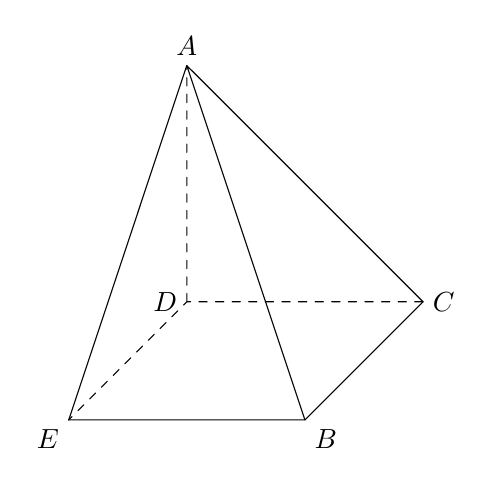
\begin{tikzpicture}[>=latex, line cap = round, line join = round, scale = 3]
    \draw (0,0) node [below left] {$E$} -- (1,0) node [below right] {$B$} --++ (45:{sqrt(2)/2}) node [right] {$C$} coordinate (C);
    \draw [dashed] (C) --++ (-1,0) node [left] {$D$} coordinate (D) -- (0,0) (D) --++ (0,1) node [above] {$A$} coordinate (A);
    \draw (A) -- (0,0) (A) -- (C) (A) -- (1,0);
\end{tikzpicture}
\end{center}
\item (003487)已知$SA$、$SB$是圆锥$SO$的两条母线, $O$是底面圆的圆心, 底面圆的半径为$10$, $C$是$SB$中点, $\angle AOB=60^\circ$, $AC$与底面所成角为$45^\circ$, 求此圆锥的侧面积和体积.
\item (003488)已知长方体$ABCD-A_1B_1C_1D_1$中, $AB=BC=4$, $CC_1=2$, 则直线$BC_1$和平面$DBB_1D_1$所成角的大小为\blank{50}.
\item (003489)设$ABCD$是一个正方形, $PA\perp$平面$ABCD$, $PA=AB$, 则:\\
(1) 直线$AB$与$PC$所成的角的大小为\blank{50};\\
(2) 直线$PC$与平面$ABCD$所成的角的大小为\blank{50};\\
(3) 二面角$P-BC-A$的大小为\blank{50}.
\item (003490)棱长为$1$的正四面体$ABCD$中, $E,F,G$分别是棱$AB,AC,AD$的中点.\\
(1) 点$A$和平面$BCD$的距离为\blank{50};\\
(2) 直线$EF$和平面$BCD$的距离为\blank{50};\\
(3) 平面$EFG$和平面$BCD$的距离为\blank{50};\\
(4) 异面直线$AD$和$BC$的距离为\blank{50}.
\item (003491)在正四棱锥$P-ABCD$中, 若侧面与底面所成二面角的大小为$60^\circ$, 则异面直线$PA$与$BC$所成角的大小为\blank{50}.
\item (003492)如图, 有一种多面体的饰品, 其表面由$6$个正方形和$8$个正三角形组成, 直线$AB$与$CD$所成角的大小是\blank{50}.
\begin{center}
    \begin{tikzpicture}[>=latex, line cap = round, line join = round,scale =0.5]
        \draw (0,0) coordinate(M) (4,0) coordinate (N) (N) ++ (50:2) coordinate (P) (M) ++ (50:2) coordinate (Q);
        \draw (M) ++ (0,4) coordinate (M1) (N) ++ (0,4) coordinate (N1) (P) ++ (0,4) coordinate (P1) (Q) ++ (0,4) coordinate (Q1);
        \draw ($(N)!0.5!0:(P)$) coordinate (D) node [right] {$D$} -- ($(M)!0.5!0:(N)$) coordinate (D1) -- ($(M)!0.5!0:(Q)$) coordinate (D2);
        \draw [dashed] (D2) -- ($(P)!0.5!0:(Q)$) coordinate (D3) -- (D);
        \draw ($(P)!0.5!0:(P1)$) coordinate (C) node [right] {$C$} -- (D) -- ($(N)!0.5!0:(N1)$) coordinate (C1) -- (D1) -- ($(M)!0.5!0:(M1)$) coordinate (C2) -- (D2);
        \draw [dashed] (D2) -- ($(Q1)!0.5!0:(Q)$) coordinate (C3) -- (D3) -- (C);
        \draw ($(N1)!0.5!0:(P1)$) coordinate (A1) -- ($(P1)!0.5!0:(Q1)$) coordinate (B) node [above] {$B$} -- ($(M1)!0.5!0:(Q1)$) coordinate (A) node [left] {$A$} 
        -- ($(M1)!0.5!0:(N1)$) coordinate (B1) --  cycle;
        \draw (C) -- (A1) -- (C1) -- (B1) -- (C2) -- (A);
        \draw [dashed] (A) -- (C3) -- (B) -- (C);  
    \end{tikzpicture}
\end{center}
\item (003493)山坡与平面成$30^\circ$角, 坡面上有一条与坡脚水平线成$30^\circ$的直线小路. 某人沿小路上坡走了一段路程后升高了$100$米, 则此人行走的路程为\blank{50}米.
\item (003494)已知正三棱锥$P-ABC$的体积为$72\sqrt 3$, 侧面与底面所成的二面角的大小为$60^\circ$.
\begin{center}
    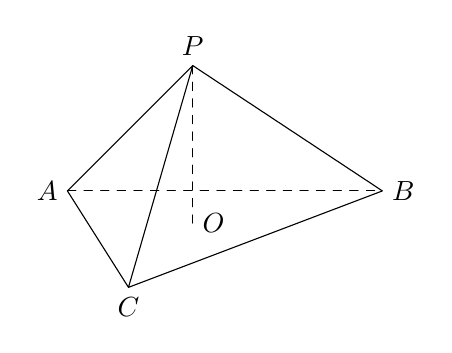
\begin{tikzpicture}[>=latex, line cap = round, line join = round]
        \draw (0,0) coordinate (A) node [left] {$A$} (4,0) coordinate (B) node [right] {$B$};
        \draw (2,0) ++ (225:{sqrt(3)}) coordinate (C) node [below] {$C$};
        \draw (2,0) ++ (225:{sqrt(3)/3}) coordinate (O) node [right] {$O$};
        \draw (O) ++ (0,2) coordinate (P) node [above] {$P$};
        \draw (A) -- (C) -- (B) -- (P) -- (A) (P) -- (C);
        \draw [dashed] (A) -- (B) (P) -- (O);
     \end{tikzpicture}
\end{center}
(1) 证明: $PA\perp BC$;\\
(2) 求底面中心$O$到侧面的距离;\\
(3) 求正三棱锥$P-ABC$的表面积.
\item (003495)如图, 在直三棱柱$ABC-A_1B_1C_1$中, $AA_1=BC=AB=2$, $AB\perp BC$.
\begin{center}
    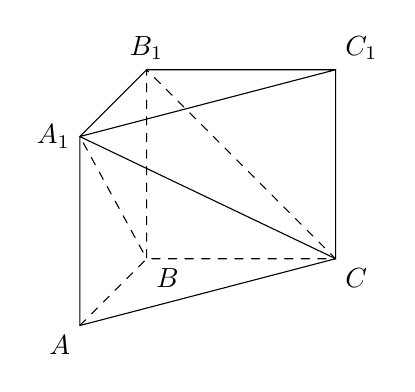
\begin{tikzpicture}[>=latex, line cap = round, line join = round, scale = 0.6]
        \draw (0,0) node [below left] {$A$} coordinate (A) ++ (45:2) node [below right] {$B$} coordinate (B) 
        ++ (4,0) node [below right] {$C$} coordinate (C);
        \draw (A) ++ (0,4) coordinate (A1) node [left] {$A_1$};
        \draw (B) ++ (0,4) coordinate (B1) node [above] {$B_1$};
        \draw (C) ++ (0,4) coordinate (C1) node [above right] {$C_1$};
        \draw (A1) -- (B1) -- (C1) -- cycle;
        \draw (C1) -- (C) -- (A) -- (A1) -- (C);
        \draw [dashed] (A) -- (B) -- (C) -- (B1)-- (B) -- (A1);
    \end{tikzpicture}
\end{center}
(1) 求直线$A_1C$和直线$B_1C_1$所成的角的大小;\\
(2) 求二面角$C-A_1B_1-C_1$的大小;\\
(3) 求点$A$到平面$A_1BC$的距离.
\item (003496)已知$ABCD-A_1B_1C_1D_1$是底面边长为$1$的正四棱柱.
\begin{center}
    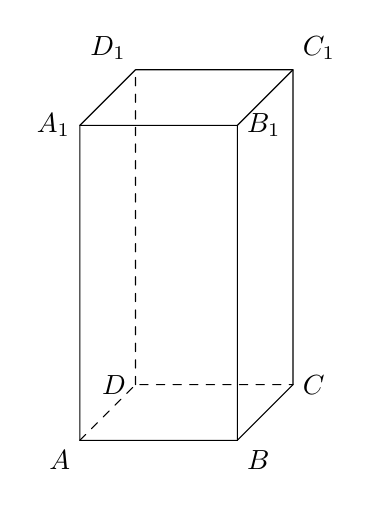
\begin{tikzpicture}[>=latex, line cap = round, line join = round, scale = 2]
        \draw (0,0) node [below left] {$A$} coordinate (A) --++ (1,0) node [below right] {$B$} coordinate (B) --++ (45:{1/2}) node [right] {$C$} coordinate (C)
        --++ (0,2) node [above right] {$C_1$} coordinate (C1)
        --++ (-1,0) node [above left] {$D_1$} coordinate (D1) --++ (225:{1/2}) node [left] {$A_1$} coordinate (A1) -- cycle;
        \draw (A) ++ (1,2) node [right] {$B_1$} coordinate (B1) -- (B) (B1) --++ (45:{1/2}) (B1) --++ (-1,0);
        \draw [dashed] (A) --++ (45:{1/2}) node [left] {$D$} coordinate (D) --++ (1,0) (D) --++ (0,2);
    \end{tikzpicture}
\end{center}
(1) 设$AB_1$与面$A_1B_1C_1D_1$所成的角的大小为$\alpha$, 二面角$A-B_1D_1-A_1$的大小为$\beta$, 试求$\alpha$与$\beta$的一个(非平凡的)等式关系;\\
(2) 若点$C$到平面$AB_1D_1$的距离为$\dfrac 43$, 求该正四棱柱的高;\\
(3) 若正四棱柱的高为$2$, 求四面体$A_1C_1BD$的体积.
\item (003497)在底面边长为$2$的正三棱锥$V-ABC$中, $E$是$BC$的中点, 若三角形$VAE$的面积为$\dfrac 14$, 则侧棱$VA$与底面所成的角的大小为\blank{50}.
\item (003498)在棱长为$2$的正方体$ABCD-A_1B_1C_1D_1$中, $O$为$BD$的中点.\\
(1) 直线$AB_1$与直线$C_1O$所成的角的大小为\blank{50};\\
(2) 直线$BD_1$与平面$A_1B_1C_1D_1$所成的角的大小为\blank{50};\\
(3) 二面角$C_1-BD-A$的大小为\blank{50}.
\item (003499)在棱长为$2$的正方体$ABCD-A_1B_1C_1D_1$中, $O$为$BD$的中点.\\
(1) 点$B$到平面$AB_1D_1$的距离为\blank{50};\\
(2) 直线$C_1O$和平面$AB_1D_1$的距离为\blank{50};\\
(3) 平面$AB_1D_1$和平面$C_1BD$的距离为\blank{50};\\
(4) 异面直线$BD$与$CC_1$的距离为\blank{50}.
\item (003500)在四棱锥$P-ABCD$中, 底面是边长为$2$的菱形. $\angle DAB=60^\circ$, 对角线$AC$与$BD$相交于点$O$, $PO\perp$平面$ABCD$, $PB$与平面$ABCD$所成的角的大小为$60^\circ$.
\begin{center}
    \begin{tikzpicture}[>=latex, line cap = round, line join = round, scale = 1.3]
        \draw ({-sqrt(3)},0) coordinate (A) node [left] {$A$};
        \draw ({sqrt(3)},0) coordinate (C) node [right] {$C$};
        \draw (45:0.5) coordinate (D) node [above right] {$D$};
        \draw (225:0.5) coordinate (B) node [below left] {$B$};
        \draw (0,{sqrt(3)}) coordinate (P) node [above] {$P$};
        \draw ($(P)!0.5!(B)$) coordinate (E) node [left] {$E$};
        \draw (A) -- (B) -- (C) -- (P) -- cycle (P) -- (B);
        \draw [dashed] (D) -- (A) (D) -- (E) (D) -- (C) (D) -- (P);
    \end{tikzpicture}
\end{center}
(1) 求四棱锥$P-ABCD$的体积;\\
(2) 若$E$是$PB$的中点, 求异面直线$DE$与$PA$所成的角的大小.
\item (003501)用``$\subseteq$''连接集合$\mathbf{Z}$、$\mathbf{Q}$、$\mathbf{R}$、$\mathbf{C}$:\blank{50}.
\item (003502)设复数$z=1-2\mathrm{i}$, 则复数$z-\overline{z+1}=$\blank{50}.
\item (003503)已知$a$是实常数, 则$\dfrac{a+\mathrm{i}}{1+\mathrm{i}}$的虚部$\mathrm{Im}\dfrac{a+\mathrm{i}}{1+\mathrm{i}}=$\blank{50}.
\item (003504)若复数$z$满足$z=\mathrm{i}(2-z)$, 则$z=$\blank{50}.
\item (003505)已知$2z+|z|=1-2\mathrm{i}$, 则复数$z=$\blank{50}.
\item (003506)若纯虚数$z$的模为$2$, 则$z^2=$\blank{50}.
\item (003507)求值: $|\dfrac{(1-\mathrm{i})^{10000}(3-4\mathrm{i})^2}{(-\sqrt{3}+\mathrm{i})^{5000}}|$.
\item (003508)判断下列命题的真假, 对于假命题请至少举一个反例.
\begin{center}
    \begin{tabular}{|c|c|p{.25\textwidth}<{\centering}|}
        \hline
        命题 & 填``真''或``假'' & 反例\\ \hline
        (1) 复数$z$是实数的充要条件是$z-\overline z=0$.	& & \\ \hline
        (2) 复数$z$是纯虚数的充要条件是$z+\overline z=0$. & & \\ \hline
        (3) $z+\overline{z}$和$z\cdot \overline{z}$都是实数. & & \\ \hline
        (4) 已知$|z|=2$, 那么$z=\pm 2$或$\pm 2\mathrm{i}$. & & \\ \hline
    \end{tabular}
\end{center}
\item (003509)求当$a$为何实数时, 复数$z=\dfrac{a^2+a-30}{a+2}+(a^2-3a-10)\mathrm{i}$分别是:\\
(1) 实数;\\
(2) 虚数;\\
(3) 纯虚数;\\
(4) 零.
\item (003510)已知复数$w$满足$w-4=(3-2w)\mathrm{i}$, $z=\dfrac 5w+|w-2|$, 求$|z|$.
\item (003511)已知$z$是虚数, $w=z+\dfrac{1}{z}$是实数, 且$-1<w<2$.\\
(1) 求$|z|$的值及$z$的实部取值范围;\\
(2) 设$u=\dfrac{1-z}{1+z}$, 求证: $u$为纯虚数;\\
(3) 求$w-u^2$的最小值.
\item (003512)复数$2-3\mathrm{i}$的虚部为\bracket{20}.
\fourch{$-3$}{$-3\mathrm{i}$}{$3$}{$3\mathrm{i}$}
\item (003513)若复数$z$满足$z+2\overline z=3-\mathrm{i}$, 则$z=$\blank{50}.
\item (003514)设$b$是实数, 若$\dfrac{1+\mathrm{i}}{2+b\mathrm{i}}+\dfrac 12$的实部与虚部相等, 则$b=$\blank{50}.
\item (003515)设$a$是实数, 若$|\dfrac{(1+\mathrm{i})^3(a-\mathrm{i})^2}{\sqrt{2}(a-3\mathrm{i})^2}|=\dfrac 32$, 则$a=$\blank{50}.
\item (003516)下列命题中正确的有:\blank{50}.\\
(1) 设$z_1,z_2$为复数, 若$z_1^2+z_2^2=0$, 则$z_1+z_2=0$;\\
(2) 设$z_1,z_2$为复数, $z_1\cdot z_2=0$的充要条件为$z_1=0$或$z_2=0$;\\
(3) 若$z_1+z_2>0$, 那么$z_1>-z_2$;\\
(4) 若$|z|\le 1$, 则$-1\le z\le 1$;\\
(5) 若$z\in \mathbf{C}$, 那么$|z^2|=|z|^2$;\\
(6) 若$z\in \mathbf{C}$, 那么$|z|=\sqrt{z^2}$.
\item (003517)已知虚数$z$使得$m=z+\dfrac 4z$是实数.\\
(1) 求$|z|$的值;\\
(2) 求$m$的取值范围;\\
(3) 若$(z+2)(1+\mathrm{i})$是纯虚数, 求$z$的值.\\
\item (003518)已知$|z_1|=2$, $|z_2|=3$, $|z_1+z_2|=4$, 求 $|z_1-2z_2|$.
\item (003519)复数$z$与$\overline z$在复平面内对应的点\bracket{20}.
\fourch{关于原点对称}{关于$x$轴对称}{关于$y$轴对称}{关于直线$y=x$对称}
\item (003520)若复数$z_1$、$z_2$满足$z_1+z_2=0$, 则$z_1$、$z_2$在复平面上对应的点$Z_1$、$Z_2$\bracket{20}.
\fourch{关于原点对称}{关于$x$轴对称}{关于$y$轴对称}{关于直线$y=x$对称}
\item (003521)满足$\begin{cases} |z-\mathrm{i}|\le 1, \\ \mathrm {Re}z\ge 0 \end{cases}$的复数、在复平面内对应点所构成图形的面积为\blank{50}.
\item (003522)平行四边形$ABCD$的三个顶点$A,B,C$依次对应复数$z_1=0$, $z_2=1+\mathrm{i}$, $z_3=-1+2\mathrm{i}$, 则点$D$对应的复数为\blank{50}.
\item (003523)设$z=a+b\mathrm{i}$($a,b\in\mathbf{R}$), 则$\mathrm{i}\cdot \overline{z}$所表示的点、关于直线$y=x$对称的点的复数表示为\blank{50}.
\item (003524)满足下列条件的复数$z$所对应点的轨迹是什么? 在空格内填入轨迹类型和直角坐标系下方程.\\
例子: (0) $|z|=1$: 圆$x^2+y^2=1$;\\
(1) $|z-\mathrm{i}|=|z+\mathrm{i}|$:\blank{50};\\
(2) $|z+1|=1$:\blank{50};\\
(3) $|z-5|+|z+5|=12$:\blank{50};\\
(4) $|z-1|+|z+1|=2$:\blank{50};\\
(5) $|z-2\mathrm{i}|-|z+2\mathrm{i}|=2$:\blank{50}.
\item (003525)已知$|z_1|=1$, $|z_2|=\sqrt{3}$, $|z_1-z_2|=2$, 则$|z_1+z_2|=$\blank{50}.
\item (003526)已知$|z|=|z-1|=1$, 则$z=$\blank{50}.
\item (003527)(1) 已知$|z|=1$, 求$|z-2|$的取值范围;\\
(2) 已知$|z-\mathrm{i}|=3$, 求$|z+1|$的取值范围.
\item (003528)设复数$z$满足$|z+1-2\mathrm{i}|=3$, 复数$w=4z-\mathrm{i}+1$, 求复数$w$对应点的轨迹.
\item (003529)由方程:$|z|^2-8|z|+15=0$所确定的复平面内对应的点所组成的图形是\bracket{20}.
\fourch{四个点}{四条直线}{一个圆}{ 两个圆}
\item (003530)已知$|z-2|=|z-1+\mathrm{i}|$, 则复数$z$在复平面上所对应的点$Z$的轨迹是\blank{50}.
\item (003531)满足方程$z\overline{z}-z-\overline{z}=8$的复数$z$在复平面上所对应的点的轨迹是\blank{50}.
\item (003532)设复数$z$满足$|z+1|+|z-1|=2$, 则$|z-4-\mathrm{i}|$的最小值为\blank{50}.
\item (003533)若集合$A=\{z||z+5\mathrm{i}|-|z-5\mathrm{i}|=8\}$, $B=\{z||z|=4\}$, 则$A\cap B=$\blank{50}.
\item (003534)已知复数z满足$|z-3+4\mathrm{i}|=2$,\\
(1) 求$|z+1|$的取值范围;\\
(2) 求出使$|z+1|$取最大值的$z$的值.
\item (003535)已知复数$z$满足$|z|=2$, 求复数$w=\dfrac{1+z}z$在复平面内的对应点的轨迹.
\item (003536)负实数$a$的平方根为\blank{50}.
\item (003537)$8$的立方根为\blank{50}.
\item (003538)计算: $1+\mathrm{i}+\mathrm{i}^2+\cdots+\mathrm{i}^{100}=$\blank{50}.
\item (003539)设$\omega=-\dfrac 12+\dfrac{\sqrt 3}2\mathrm{i}$, 则$1+\omega+\omega^2+\omega^3+\cdots+\omega^{2000}=$\blank{50}.
\item (003540)计算: $(1+\mathrm{i})^{10000}=$\blank{50}.
\item (003541)(1) $2x^2+4x+1=0$的解为\blank{50};\\
(2) 复数集中分解因式: $2x^2+4x+1=$\blank{50}.
\item (003542)已知关于$x$的实系数一元二次方程$ax^2+bx+c=0\ (a\ne 0)$在复数集中的两个根为$\alpha,\beta$, 下列命题中正确的有\blank{50}.\\
\textcircled{1} $\alpha$和$\beta$互为共轭复数;\\
\textcircled{2} $\alpha +\beta =-\dfrac ba$, $\alpha \beta =\dfrac ca$;\\
\textcircled{3} $\alpha$和$\beta$分别为$\dfrac{-b\pm \sqrt{b^2}-4ac}{2a}$;\\
\textcircled{4} $|\alpha -\beta|^2=(\alpha-\beta)^2$;\\
\textcircled{5} $ax^2+bx+c=a(x-\alpha)(x-\beta)$.
\item (003543)求$-\dfrac{13}4+2\sqrt 3\mathrm{i}$的平方根.
\item (003544)设$p,q\in \mathbf{R}$, 若关于$x$的方程$2x^2+px+q=0$的一个根为$-3+2\mathrm{i}$, 求$p,q$的值.
\item (003545)设$m$是实数, 关于$x$的方程$x^2-mx+1=0$的两个复数根为$\alpha,\beta$. 若$|\alpha-\beta|=1$, 求$m$的值.
\item (003546)设$m$是实数, 若关于$x$的方程$2x^2+3mx+m^2-m=0$至少有一个模为$1$的根, 求$m$的值.
\item (003547)实数$-2$的平方根为\blank{50}.
\item (003548)实数$-1$的立方根为\blank{50}.
\item (003549)若复数$a+b\mathrm{i}$($a,b\in \mathbf{R}$)是关于$x$的实系数方程$x^2+px+q=0$的两根, 则$p=$\blank{50}, $q=$\blank{50}.
\item (003550)计算: $\mathrm{i}\cdot\mathrm{i}^2\cdot\mathrm{i}^3\cdot \cdots \cdot \mathrm{i}^{100}=$\blank{50}.
\item (003551)设$m$是实数, 关于$x$的方程$x^2-2\sqrt 2x+m=0$的两个复数根为$\alpha,\beta$.\\
(1) 若$|\alpha-\beta|=3$, 求实数$m$的值;\\
(2) 若$|\alpha|+|\beta|=3$, 求实数$m$的值.
\item (003552)设$m$是实数, 若$\alpha$是实系数一元二次方程$mx^2+x+1=0$的根, 且满足$|\alpha+1|=1$, 求$m$的取值范围.
\item (003553)已知关于$x$的方程$x^2+(4+\mathrm{i})x+3+p\mathrm{i}=0$($p\in \mathbf{R}$)有实数根, 求$p$的值, 并解这个方程.
\item (003554)若矩阵$\begin{pmatrix}a & b \\ c & d\end{pmatrix}$为$n$阶单位阵, 则$a-b-c+d+n=$\blank{50}.
\item (003555)方程组$\begin{cases} 2x+y=7, \\ x-y=2 \end{cases}$的系数行列式的值为\blank{50}, 系数矩阵的行向量为\blank{50}.
\item (003556)行列式$\begin{vmatrix}1 & 2 & 0 \\ 1 & 5 & 1 \\ 1 & 8 & 0 \end{vmatrix}=$\blank{50}.
\item (003557)在三阶行列式$\begin{vmatrix}1 & 2 & 3 \\4 & 5 & 6  \\7 & 8 & -9 \end{vmatrix}$中, 元素$6$的余子式为\blank{50}, 元素$8$的代数余子式的值为\blank{50}.
\item (003558)关于$x$、$y$的方程组$\begin{cases} mx+2y=m+4, \\ 2x+my=m \end{cases}$无解, 则实数$m=$\blank{50}.
\item (003559)设$m$是实数, 解关于$x,y$的方程组$\begin{cases} mx+2y=m, \\ x+(m-1)y=-m. \end{cases}$
\item (003560)已知关于$x,y,z$的方程组$\begin{cases} x+y+z=1, \\ x+y+az=1, \\ x+ay+a^2z=2, \end{cases}$其中$a\in \mathbf{R}$.\\
(1) 若关于$x$、$y$的方程组$\begin{cases} a_1x+b_1y=c_1, \\ a_2x+b_2y=c_2 \end{cases}$可以用矩阵记号$\begin{pmatrix}
 a_1 & b_1 \\ a_2 & b_2  \end{pmatrix}\begin{pmatrix}    x  \\ y  \end{pmatrix}=\begin{pmatrix} c_1 \\ c_2 \end{pmatrix}$来表示, 请试给出上述三元一次方程组的矩阵表示;\\
(2) 用行列式的方法解此方程组.
\item (003561)已知平面直角坐标系内点$A(0,3)$, 点$B(2,0)$, 点$C(5,\lambda)$.\\
(1)	若三角形$ABC$面积为$10$, 求$\lambda$的值;\\
(2)	若$A,B,C$三点共线, 求$\lambda$的值.
\item (003562)行列式$\begin{vmatrix} 1 & 3 & 0  \\ 4 & 5 & 1  \\ 7 & 8 & 2 \end{vmatrix}$中, 元素$4$的余子式的值为\blank{50}, 元素$3$的代数余子式的值为\blank{50}.
\item (003563)将 $a\begin{vmatrix} 1 & 2 \\0 & 4 \end{vmatrix}+b \begin{vmatrix}
-1 & 3  \\ 0 & 4 \end{vmatrix}+c \begin{vmatrix}
-1 & 3  \\ 1 & 2 \end{vmatrix}$化为一个三阶行列式: $\begin{vmatrix}a & -1 & 3 \\ \blank{10} & \blank{10} & \blank{10} \\ \blank{10} & \blank{10} & \blank{10}\end{vmatrix}$.
\item (003564)若关于$x$、$y$的方程组$\begin{cases} mx+y=-1,\\ x+my=1 \end{cases}$有解, 则实数$m$的取值范围为\blank{50}.
\item (003565)关于$x,y,z$的方程组$\begin{cases} x+y+az=1, \\ x+ay+z=a, \\ x-y+z=3 \end{cases}$的增广矩阵是\blank{50}; 若此方程组有唯一解, 则实数a的取值范围为\blank{50}.
\item (003566)设$m$是实数, 用行列式的方法解关于$x$、$y$的方程组$\begin{cases} (m+1)x-(2m-1)y=3m, \\ (3m+1)x-(4m-1)y=5m+4. \end{cases}$
\item (003567)若$m\in \mathbf{N}^*$, $m<27$, 则$(27-m)(28-m)\cdots (34-m)=$\blank{50}(用排列数表示).
\item (003568)$540$的不同的正约数共有\blank{50}个, 这些正约数中是$3$的倍数的有\blank{50}个.
\item (003569)$3000$和$8000$之间有\blank{50}个能被5整除的且在数位上无重复数字的数.
\item (003570)平面上有$10$个点, 其中除有$4$个点在同一条直线上外, 不再有其它三点共线的情形, 经过这些点可以确定\blank{50}条直线.
\item (003571)从$5$男$3$女共$8$名学生中选出队长$1$人, 副队长$1$人, 普通队员$2$人组成$4$人志愿者服务队, 要求服务队中至少有$1$名女生, 共有\blank{50}种不同的选法(用数字作答).
\item (003572)$(2x-\dfrac 1{\sqrt x})^6$的展开式中第三项的二项式系数为\blank{50}, 第三项的系数为\blank{50}.
\item (003573)化简: (1) $1+2\mathrm{C}_n^1+4\mathrm{C}_n^2+\cdots+2^n\mathrm{C}_n^n=$\blank{50};\\
(2) $\mathrm{C}_3^3+\mathrm{C}_4^3+\mathrm{C}_5^3+\cdots+\mathrm{C}_n^3=$\blank{50}.
\item (003574)随机抽取$9$个同学中, 至少有$2$个同学在同一月出生的概率是\blank{50}(默认每月天数相同, 结果精确到$0.001$).
\item (003575)从一副$52$张扑克牌中随机抽取$4$张牌.\\
(1) 在放回抽取的情形下, $4$张牌都是A的概率为\blank{50};
(2) 在不放回抽取的情形下, $4$张牌都是A的概率为\blank{50}.
\item (003576)*已知总体的各个体的值由小到大依次为$2,3,3,7,a,b,12, 13.7,18.3,20$, 且总体的中位数为$10.5$. 若要使该总体的方差最大, 则$a$=\blank{50}, $b$=\blank{50}.
\item (003577)有$3$名男生, $4$名女生, 全体排成一行, 在下列不同的要求下, 分别求不同排列的方法数:\\
(1) 男生必须排在一起;\\
(2) 任意两个男生都不相邻;\\
(3) 甲不在最左边, 乙不在最右边;\\
(4) 甲必须站在乙的左方(不一定相邻);\\
(5) 其中甲、乙、丙三人从左至右的顺序不变(都不一定相邻).
\item (003578)求二项式$(2+x^2)^{32}$展开式中,\\
(1) 二项式系数最大的项;\\
(2) 系数最大的项;\\
(3) 所有项的系数之和.
\item (003579)某中学共有学生$2000$名, 各年级男、女生人数如下表.
\begin{center}
    \begin{tabular}{|c|c|c|c|}
        \hline
        & 一年级 & 二年级 & 三年级\\ \hline
        女生 & $373$ & $x$ & $y$ \\ \hline
        男生 & $377$ & $370$ & $z$ \\ \hline
    \end{tabular}
\end{center}
已知在全校学生中随机抽取$1$名, 抽到二年级女生的概率是0.19.\\
(1) 求$x$的值;\\
(2) 现用分层抽样的方法在全校抽取$48$名学生, 问应在三年级抽取多少名?\\
(3) 已知$y\ge 245$, $z\ge 245$, 求三年级中女生比男生多的概率.
\item (003580)已知$\mathrm{C}_{18}^{2x}=\mathrm{C}_{18}^{x+3}$, 则$x$=\blank{50}.
\item (003581)用$0$、$1$、$2$、$3$、$4$、$5$组成的无重复数字的数中比$240135$大的数有\blank{50}个.
\item (003582)甲、乙、丙三人值周一至周六的班, 每人值两天班, 若甲不值周一、乙不值周六, 则可排出不同的值班表数为\blank{50}.
\item (003583)在$(\sqrt[3]x-\dfrac 1{2\cdot \sqrt[3]x})^{10}$的二项展开式中, 常数项是\blank{50}; 含$x^2$项的二项式系数是\blank{50}; 含$x^2$项的系数是\blank{50}.
\item (003584)设$1+(1+x)+(1+x)^2+\cdots+(1+x)^{2021}=a_0+a_1x+a_2x^2+\cdots +a_{2021}x^{2021}$, 则$a_{100}+a_{101}=$\blank{50}.
\item (003585)已知$a,b\in \{-3,-2,-1,1,2,3\}$且$a\ne b$, 则复数$z=a+b\mathrm{i}$对应点在第二象限的概率为\blank{50}(用最简分数表示).
\item (003586)盒子中装着标有$1,2,3,4$的卡片各两张, 从盒中任取$3$张, 每张卡片被抽到的概率相等, 则抽出的$3$张卡片上的数字互不相同的概率为\blank{50}.
\item (003587)某区有$200$名学生参加数学竞赛, 随机抽取10名学生成绩如下:
\begin{center}
    \begin{tabular}{|c|c|c|c|c|c|c|}
        \hline
        成绩 & $40$ & $50$ & $60$ & $70$ & $80$ & $90$\\ \hline
        人数 & $2$ & $1$ & $2$ & $2$ & $1$ & $2$ \\ \hline        
    \end{tabular}
\end{center}
则总体标准差的点估计值是\blank{50}.(精确到$0.01$)
\item (003588)某学校组织学生参加英语测试, 成绩的频率分布直方图如图所示, 数据的分组依$[20,40)$, $[40,60)$, $[60,80)$, $[80,100)$, 若低于$60$分的人数是$15$人, 则该班的学生人数是\blank{50}.
\begin{center}
\begin{tikzpicture}[>=latex, line cap = round, line join = round, scale = 1.2]
    \draw [->] (-2,0) -- (6.5,0) node [below] {成绩(分)};
    \draw [->] (0,-1) -- (0,3) node [left] {$\dfrac{\text{频率}}{\text{组距}}$};
    \draw (0,0) node [below left] {$O$};
    \draw (1,0) -- (1,0.5) -- (2,0.5);
    \draw (2,0) -- (2,1) -- (3,1);
    \draw (3,0) -- (3,2) -- (4,2) -- (4,0);
    \draw (4,1.5) -- (5,1.5) -- (5,0);
    \draw [dashed] (0,0.5) -- (1,0.5) (0,1) -- (2,1) (0,1.5) -- (4,1.5) (0,2) -- (3,2);
    \foreach \i in {20,40,...,100}
        \draw ({\i/20},0) node [below] {$\i$};
    \foreach \i in {0.005,0.01,0.015,0.02}
        \draw (-1.2,{\i*100}) node [right] {$\i$};
\end{tikzpicture}
\end{center}
\item (000001)用列举法表示下列集合:\\
(1) 十二生肖组成的集合;\\
(2) 中国国旗上所有颜色组成的集合.
\item (000002)用描述法表示下列集合:\\
(1) 平面直角坐标系中第一象限的角平分线上的所有点组成的集合;\\
(2) $3$的所有倍数组成的集合.
\item (000003)(1) 若$\alpha$: $x^2-5x+6=0$, $\beta$: $x=2$, 则$\alpha$是$\beta$的\blank{50}条件;
(2) 若$\alpha$: 四边形$ABCD$是正方形, $\beta$: 四边形$ABCD$的两条对角线互相垂直平分, 则$\alpha$是$\beta$的\blank{50}条件.
\item (000004)已知方程$x^2+px+4=0$的所有解组成的集合为$A$, 方程$x^2+x+q=0$的所有解组成的集合为$B$, 且$A\cap B=\{4\}$. 求集合$A\cup B$的所有子集.
\item (000005)已知集合$A=(-2, 1)$, $B=(-\infty, -2)\cup [1, +\infty)$. 求: $A\cup B$, $A\cap B$.
\item (000006)已知全集$U=(-\infty, 1)\cup [2, +\infty)$, 集合$A=(-1, 1)\cup [3, +\infty)$. 求$\overline{A}$.
\item (000007)已知集合$A=\{x|x^2+px+q=0\}$, $B=\{x|x^2-x+r=0\}$, 且$A\cap B=\{-1\}$, $A\cup B=\{-1, 2\}$. 求实数$p$、$q$、$r$的值.
\item (000008)设$a$是实数. 若$x=1$是$x>a$的一个充分条件, 则$a$的取值范围为\blank{50}.
\item (000009)已知陈述句$\alpha$是$\beta$的充分非必要条件. 若集合$M=\{x|x\text{满足}\alpha\}$, $N=\{x|x\text{满足}\beta\}$, 则$M$与$N$的关系为\bracket{20}.
\fourch{$M\subset N$}{$M\supset N$}{$M=N$}{$M\cap N=\varnothing$}
\item (000010)证明: 若梯形的对角线不相等, 则该梯形不是等腰梯形.
\item (000011)若集合$M=\{a|a=x+\sqrt2y, x,y\in \mathbf{Q}\}$, 则下列结论正确的是\bracket{20}.
\fourch{$M\subseteq \mathbf{Q}$}{$M=\mathbf{Q}$}{$M\supset \mathbf{Q}$}{$M\subset \mathbf{Q}$}
\item (000012)若$\alpha$是$\beta$的必要非充分条件, $\beta$是$\gamma$的充要条件, $\gamma$是$\delta$的必要非充分条件, 则$\delta$是$\alpha$的\blank{50}条件, $\gamma$是$\alpha$的\blank{50}条件.
\item (000013)已知全集$U=\{x|x\text{为不大于}20\text{的素数}\}$. 若$A\cap \overline{B}=\{3, 5\}$, $\overline{A}\cap B=\{7, 19\}$, $\overline{A\cup B}=\{2, 17\}$, 则A=\blank{50} , B=\blank{50}.
\item (000014)已知集合$P=\{x|-2\le x\le 5\}$, $Q=\{x|x\ge k+1\text{且}x\le 2k-1\}$, 且$Q\subseteq P$. 求实数$k$的取值范围.
\item (000015)已知全集$U=\mathbf{R}$, 集合$A=\{x|x\le a-1\}$, $B=\{x|x>a+2\}$, $C=\{x|x<0\text{或}x\ge 4\}$, 且$\overline{A\cup B}\subseteq C$. 求实数$a$的取值范围.
\item (000016)已知集合$A=\{x|(a-1)x^2+3x-2=0\}$. 是否存在这样的实数$a$, 使得集合$A$有且仅有两个子集? 若存在, 求出实数$a$的值及对应的两个子集; 若不存在, 说明理由.
\item (000017)证明: $\sqrt[3]{2}$是无理数.
\item (000018)设$a,b$是正整数. 求证: 若$ab-1$是$3$的倍数, 则$a$与$b$被$3$除的余数相同.
\item (000019)已知非空数集$S$满足: 对任意给定的$x,y\in S$($x,y$可以相同), 有$x+y\in S$且$x-y\in S$.\\
(1) 哪个数一定是$S$中的元素? 说明理由;\\
(2) 若$S$是有限集, 求$S$;\\
(3) 若$S$中最小的正数为$5$, 求$S$.
\item (000020)设一元二次方程$2x^2-6x-3=0$的两个实根为$x_1,x_2$, 求下列各式的值:\\
(1) $(x_1+1)(x_2+1)$;\\
(2) $(x_1^2-1)(x_2^2-1)$.
\item (000021)设$a>b>0$, 比较$\dfrac{b+2a}{a+2b}$与$\dfrac ab$的值的大小.
\item (000022)已知$x>y$, 求证: $x^3-y^3>x^2y-xy^2$.
\item (000023)若关于$x$的不等式$(a+1)x-a<0$的解集为$(2,+\infty)$, 求实数$a$的值, 并求不等式$(a-1)x+3-a>0$的解集.
\item (000024)解下列一元二次不等式:\\
(1) $-x^2+11<-2x-4$;\\
(2) $3x^2<13x+10$;\\
(3) $6x+2\ge 5x^2$;\\
(4) $x^2\le 8(1-x)$;\\
(5) $-x^2\ge 9(9-2x)$;\\
(6) $3(x-3)\le x^2$.
\item (000025)试写出一个二次项系数为$1$的一元二次不等式, 使它的解集分别为:\\
(1) $(-\infty, \sqrt 2)\cup  (\sqrt 2, +\infty)$;\\
(2) $[2-\sqrt 3, 2+\sqrt 3]$.
\item (000026)求不等式$5\le x^2-2x+2<26$的所有正整数解.
\item (000027)解下列分式不等式:\\
(1) $\dfrac{2x+1}{x+7}>-3$;\\
(2) $\dfrac{3x}{x^2+2}\ge 1$.
\item (000028)设关于$x$的不等式$a_1x^2+b_1x+c_1>0$与$a_2x^2+b_2x+c_2>0$的解集分别为$A$、$B$,
试用集合运算表示下列不等式组的解集:\\
(1) $\begin{cases} a_1x^2+b_1x+c_1>0, \\ a_2x^2+b_2x+c_2>0;\end{cases}$\\
(2) $\begin{cases} a_1x^2+b_1x+c_1\le 0, \\ a_2x^2+b_2x+c_2>0;\end{cases}$\\
(3) $\begin{cases} a_1x^2+b_1x+c_1\le 0, \\ a_2x^2+b_2x+c_2\le 0.\end{cases}$
\item (000029)解下列含绝对值的不等式:\\
(1) $|2x-1|\le x$;\\
(2) $|2x+1|+|x-2|<8$.
\item (000030)已知$a$、$b$是正数, 求证: $\sqrt{(1+a)(1+b)}\ge 1+\sqrt{ab}$.
\item (000031)如图, 在直角三角形$ABC$中, $AD$垂直于斜边$BC$, 且垂足为$D$. 设$BD$及$CD$的长度分别为$a$与$b$.\\
(1) 求斜边上的高$AD$与中线$AE$的长;\\
(2) 用不等式表示斜边上的高$AD$与中线$AE$长度的大小关系.
\begin{center}
    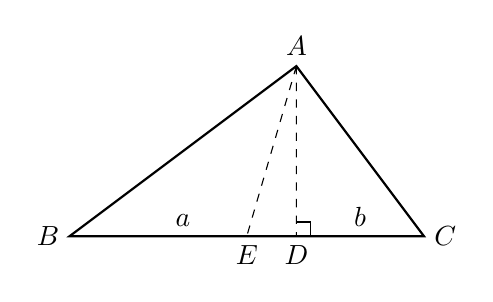
\begin{tikzpicture}[scale = 1.8]
        \draw [thick] (0,0) node [left] {$B$} -- (2.5,0) node [right] {$C$} -- (1.6,1.2) node [above] {$A$} -- cycle;
        \draw [dashed] (1.6,1.2) -- (1.6,0) node [below] {$D$} (1.6,1.2) -- (1.25,0) node [below] {$E$};
        \draw [thin] (1.7,0) -- (1.7,0.1) -- (1.6,0.1);
        \draw (0.8,0) node [above] {$a$} (2.05,0) node [above] {$b$};
    \end{tikzpicture}
\end{center}
\item (000032)如图, 已知直角梯形$ABCD$的顶点$A(a, 0)$、$B(b, 0)$位于$x$轴上, 顶点$C$、$D$落在函数$y=|x|$的图像上, $M$、$N$分别为线段$AB$、$CD$的中点, $O$为坐标原点, $Q$为线段$OC$与线段$MN$的交点.\\
(1) 求中点$M$的坐标, 以及线段$MQ$、$MN$的长度;\\
(2) 用不等式表示$MQ$、$MN$长度的大小关系.
\begin{center}
    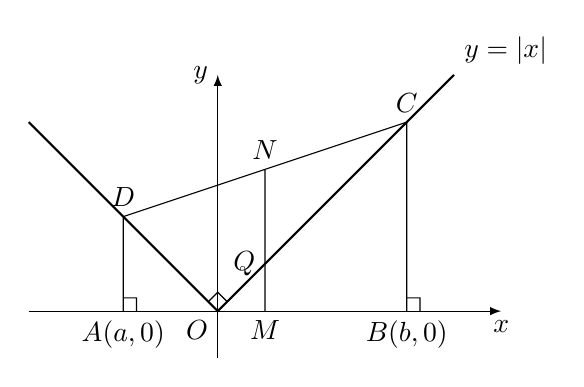
\begin{tikzpicture}[scale = 1.2,>=latex]
        \draw [->] (-2,0) -- (3,0) node [below] {$x$};
        \draw [->] (0,-0.5) -- (0,2.5) node [left] {$y$};
        \draw (0,0) node [below left] {$O$};
        \draw [thick] (-2,2) -- (0,0) -- (2.5,2.5) node [above right] {$y=|x|$};
        \draw [thin] (-0.1,0.1) -- (0,0.2) -- (0.1,0.1) (2.14,0) -- (2.14,0.14) -- (2,0.14) (-0.86,0) -- (-0.86,0.14) -- (-1,0.14);
        \draw (-1,0) node [below] {$A(a,0)$} -- (-1,1) node [above] {$D$} -- (0.5,1.5) node [above] {$N$} -- (2,2) node [above] {$C$} -- (2,0) node [below] {$B(b,0)$} (0.5,1.5) -- (0.5,0.5) node [left] {$Q$} -- (0.5,0) node [below] {$M$}; 
    \end{tikzpicture}
\end{center}
\item (000033)已知一元二次方程$x^2+px+p=0$的两个实根分别为$\alpha$、$\beta$, 且$\alpha^2$+$\beta^2=3$, 求实数$p$的值.
\item (000034)已知一元二次方程$2x^2-4x+m+3=0$有两个同号实根, 求实数$m$的取值范围.
\item (000035)设$a,b\in \mathbf{R}$, 已知关于$x$的不等式$(a+b)x+(b-2a)<0$的解集为$(1, +\infty)$, 求不等式$(a-b)x+3b-a>0$的解集.
\item (000036)解下列不等式:\\
(1) $-2< \dfrac 1{2x+1}\le 3$;\\
(2) $2<|x+1|\le 3$.
\item (000037)已知集合$A=\{x||x-a|<2\}$, $B=\{x|\dfrac{2x-1}{x+2}<1\}$, 且$A\subseteq B$. 求实数$a$的取值范围.
\item (000038)证明: 若$x>-1$, 则$x+\dfrac 1{x+1}\ge 1$, 并指出等号成立的条件.
\item (000039)设$a$、$b$为正数, 且$a+b=2$. 求$\dfrac 1a+\dfrac 1b$的最小值.
\item (000040)已知$a$、$b$、$c$都是正数, 求证: $\dfrac{b+c}{a}+\dfrac{c+a}{b}+\dfrac{a+b}{c}\ge 6$.
\item (000041)设实数$x$、$y$满足$|x+y|=1$, 求$xy$的最大值.
\item (000042)已知$a$、$b$为实数, 求证:$|a|+|b| \le |a+b| +|a-b|$, 并指出等号成立的条件.
\item (000043)已知$a$、$b$是实数,\\
(1) 求证: $a^2+ab+b^2\ge 0$, 并指出等号成立的条件;\\
(2) 求证: 如果$a>b$, 那么$a^3>b^3$.
\item (000044)解下列不等式:\\
(1) $\dfrac{3x-11}{x^2-6x+9}\le 1$;\\
(2) $|3-2x| \ge |x+1|$.
\item (000045)已知集合$A=\{x|x^2-2x-3>0\}$, $B=\{x|x^2+px+q\le 0\}$. 若$A\cup B=\mathbf{R}$, 且$A\cap B=[-2,-1)$, 求实数$p$及$q$的值.
\item (000046)已知实数$0<a<b$, 求证: $a<\dfrac{2ab}{a+b}<\sqrt{ab}<\dfrac{a+b}{2}<\sqrt{\dfrac{a^2+b^2}{2}}<b$.
\item (000047)方程$(x-1)(x-2)(x-3)=0$的三个根$1$、$2$、$3$将数轴划分为四个区间, 即$(-\infty, 1)$, $(1, 2)$, $(2, 3)$, $(3, +\infty)$. 试在这四个区间上分别考察$(x-1)(x-2)(x-3)$的
符号, 从而得出不等式$(x-1)(x-2)(x-3)>0$与$(x-1)(x-2)(x-3)<0$的解集.\\
一般地, 对$x_1$、$x_2$、$x_3\in \mathbf{R}$, 且$x_1\le x_2\le x_3$, 试分别求不等式$(x-x_1)(x-x_2)(x-x_3)>0$与$(x-x_1)(x-x_2)(x-x_3)<0$的解集(提示: $x_1$、$x_2$、$x_3$相互之间可能相等, 需要分情况讨论).
\item (000048)填空题:\\
(1) 若$x^3=5$, 则$x=$\blank{50}; 若$3^x=5$, 则$x=$\blank{50}.\\
(2) 将$\sqrt[4]{a\sqrt[3]{a}} \ (a>0)$化成有理数指数幂的形式为\blank{50}.\\
(3) 若$\log_8x=-\dfrac 23$, 则$x=$\blank{50}.\\
(4) 若$\log_a b\cdot \log_5 a=3$($a>0$且$a\ne 1$), 则$b=$\blank{50}.
\item (000049)选择题:\\
(1) 若$\lg a$与$\lg b$互为相反数, 则有\bracket{20}.
\fourch{$a+b=0$}{$ab=1$}{$\dfrac ab=1$}{以上答案均不对}
(2) 设$a>0$, 下列计算中正确的是\bracket{20}.
\twoch{$a^\frac{2}{3}\cdot a^\frac{3}{2}=a$}{$a^\frac{2}{3}\div a^\frac{3}{2}=a$}{$a^{-4}\cdot a^4=0$}{$(a^\frac{2}{3})^\frac{3}{2}=a$}
\item (000050)已知$10^\alpha=3$, $10^\beta=4$. 求$10^{\alpha+\beta}$及$10^{\alpha-\frac{\beta}2}$的值.
\item (000051)求下列各式的值:\\
(1) $\dfrac{1}{4^x+1}+\dfrac{1}{4^{-x}+1}$;\\
(2) $4^{\sqrt 2+1}\times 2^{3-2\sqrt 2}\times 8^{-\frac 23}$.
\item (000052)已知$\lg a<1$, 化简$\sqrt{\lg^2 a-\lg \dfrac{a^2}{10}}$.
\item (000053)已知$m=\log_2 10$, 求$2^m-m\lg 2-4$的值.
\item (000054)填空题:\\
(1) 若$4^x=2^{-\frac{1}{2}}$, $4^y=\sqrt[3]{32}$, 则$2x-3y=$\blank{50}.\\
(2) 若$\log_3(\log_4 x)=1$, 则$x=$\blank{50}.\\
(3) 若$3^a=7^b=63$, 则$\dfrac 2a+\dfrac 1b$的值为\blank{50}.\\
\item (000055)已知$\log_{18}9=a$, $18^b=5$, 则$\log_{36}45$等于\bracket{20}.
\fourch{$\dfrac{a+b}{2+a}$}{$\dfrac{a+b}{2-a}$}{$\dfrac{a+b}{2a}$}{$\dfrac{a+b}{a^2}$}
\item (000056)设$\log_{0.2}a>0$, $\log_{0.2}b>0$, 且$\log_{0.2}a\cdot \log_{0.2}b=1$, 求$\log_{0.2}(ab)$的最小值.
\item (000057)化简$\dfrac{(1+2^x)(1+2^{2x})(1+2^{4x})(1+2^{8x})(1+2^{16x})}{1-2^{32x}}$(其中$x\ne 0$).
\item (000058)已知$a>1$, $b>0$. 求证: 对任意给定的实数$k$, $a^{2b+k}-a^{b+k}>a^{b+k}-a^k$.
\item (000059)甲、乙两人同时解关于$x$的方程: $\log_2x+b+c\log_x2=0$. 甲写错了常数$b$, 得两根
$\dfrac 14$及$\dfrac 18$; 乙写错了常数$c$, 得两根$\dfrac 12$及$64$. 求这个方程的真正根.
\item (000060)已知$a$、$b$及$c$是不为$1$的正数, 且$\lg a+\lg b+\lg c=0$. 求证: $a^{\frac{1}{\lg b}+\frac{1}{\lg c}}\cdot b^{\frac{1}{\lg c}+\frac{1}{\lg a}}\cdot c^{\frac{1}{\lg a}+\frac{1}{\lg b}}=\dfrac{1}{1000}$.
\item (000061)填空题:\\
(1) 若点$(2, \sqrt 2)$在幂函数$y=x^a$的图像上, 则该幂函数的表达式为\blank{50}; 若点$(2, \sqrt 2)$在指数函数$y=a^x$($a>0$且$a\ne 1$)的图像上, 则该指数函数的表达式为\blank{50}; 若点$(\sqrt 2, 2)$在对数函数$y=\log_a x$($a>0$且$a\ne 1$)的图像上, 则该对数
函数的表达式为\blank{50}.\\
(2) 若幂函数$y=x^k$在区间$(0, +\infty)$上是严格减函数, 则实数$k$的取值范围为\blank{50}.\\
(3) 已知常数$a>0$且$a\ne 1$, 假设无论$a$为何值, 函数$y=a^{x-2}+1$的图像恒经过一
个定点. 则这个点的坐标为\blank{50}.
\item (000062)选择题:\\
(1) 若指数函数$y=a^x$($a>0$且$a\ne 1$)在$\mathbf{R}$上是严格减函数, 则下列不等式中, 一定能成立的是\bracket{20}.
\fourch{$a>1$}{$a<0$}{$a(a-1)<0$}{$a(a-1)>0$}
(2) 在同一平面直角坐标系中, 一次函数$y=x+a$与对数函数$y=\log_ax$($a>0$且$a\ne 1$)的图像关系可能是\bracket{20}.
\fourch{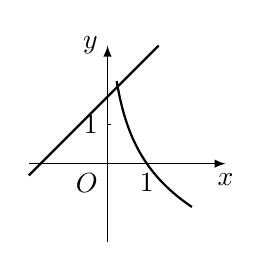
\begin{tikzpicture}[scale = 0.5,>=latex]
    \draw [->] (-2,0) -- (3,0) node [below] {$x$};
    \draw [->] (0,-2) -- (0,3) node [left] {$y$};
    \draw (0,0) node [below left] {$O$};
    \draw (0.1,1) -- (0,1) node [left] {$1$};
    \draw (1,0) node [below] {$1$};
    \draw [thick] (-2,-0.3) -- (1.3,3);
    \draw [thick,domain =-1.1:2.1,samples = 200] plot ({0.5^\x},\x);
\end{tikzpicture}
}{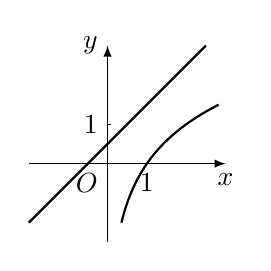
\begin{tikzpicture}[scale = 0.5,>=latex]
    \draw [->] (-2,0) -- (3,0) node [below] {$x$};
    \draw [->] (0,-2) -- (0,3) node [left] {$y$};
    \draw (0,0) node [below left] {$O$};
    \draw (0.1,1) -- (0,1) node [left] {$1$};
    \draw (1,0) node [below] {$1$};
    \draw [thick] (-2,-1.5) -- (2.5,3);
    \draw [thick,domain =1.5:-1.5,samples = 200] plot ({0.5^\x},-\x);
\end{tikzpicture}
}{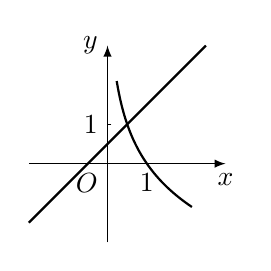
\begin{tikzpicture}[scale = 0.5,>=latex]
    \draw [->] (-2,0) -- (3,0) node [below] {$x$};
    \draw [->] (0,-2) -- (0,3) node [left] {$y$};
    \draw (0,0) node [below left] {$O$};
    \draw (0.1,1) -- (0,1) node [left] {$1$};
    \draw (1,0) node [below] {$1$};
    \draw [thick] (-2,-1.5) -- (2.5,3);
    \draw [thick,domain =-1.1:2.1,samples = 200] plot ({0.5^\x},\x);
\end{tikzpicture}
}{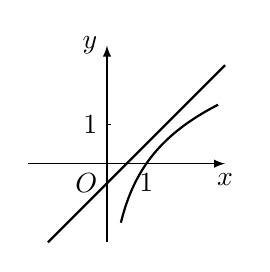
\begin{tikzpicture}[scale = 0.5,>=latex]
    \draw [->] (-2,0) -- (3,0) node [below] {$x$};
    \draw [->] (0,-2) -- (0,3) node [left] {$y$};
    \draw (0,0) node [below left] {$O$};
    \draw (0.1,1) -- (0,1) node [left] {$1$};
    \draw (1,0) node [below] {$1$};
    \draw [thick] (-1.5,-2) -- (3,2.5);
    \draw [thick,domain =1.5:-1.5,samples = 200] plot ({0.5^\x},-\x);
\end{tikzpicture}
}
\item (000063)求下列函数的的定义域:\\
(1) $y=(x-1)^{\frac 52}$;\\
(2) $y=3^{\sqrt{x-1}}$;\\
(3) $y=\lg \dfrac{1+x}{1-x}$.
\item (000064)比较下列各题中两个数的大小:\\
(1) $0.1^{0.7}$与$0.2^{0.7}$;\\
(2) $0.7^{0.1}$与$0.7^{0.2}$;\\
(3) $\log_{0.7}0.1$与$\log_{0.7}0.2$.
\item (000065)设点$(\sqrt 2, 2)$在幂函数$y_1=x^a$的图像上, 点$(-2,\dfrac 14)$在幂函数$y_2=x^b$的图像上. 当$x$取何值时, $y_1=y_2$?
\item (000066)设$a=(\dfrac 23)^x$, $b=x^{\frac 32}$及$c=\log_\frac{2}{3}x$, 当$x>1$时, 试比较$a$、$b$及$c$之间的大小关系.
\item (000067)设常数$a>0$且$a\ne 1$, 若函数$y=\log_a(x+1)$在区间$[0, 1]$上的最大值为$1$, 最小值为$0$, 求实数$a$的值.
\item (000068)如果光线每通过一块玻璃其强度要减少$10\%$, 那么至少需要将多少块这样的玻璃重叠起来, 才能使通过它们的光线强度低于原来的$\dfrac 13$?
\item (000069)填空题:\\
(1) 已知$m\in \mathbf{Z}$, 设幂函数$y=x^{m^2-4m}$的图像关于原点成中心对称, 且与$x$轴及$y$轴均无交点, 则$m$的值为\blank{50}.\\
(2) 设$a$、$b$为常数, 若$0<a<1$, $b<-1$, 则函数$y=a^x+b$的图像必定不经过第\blank{50}象限.
\item (000070)选择题:\\
(1) 若$m>n>1$, 而$0<x<1$, 则下列不等式正确的是\bracket{20}.
\fourch{$m^x<n^x$}{$x^m<x^n$}{$\log_x m>\log_x n$}{$\log_m x<\log_n x$}
(2) 在同一平面直角坐标系中, 二次函数$y=ax^2+bx$与指数函数$y=(\dfrac ba)^x$的图像关系可能为\bracket{20}.
\fourch{
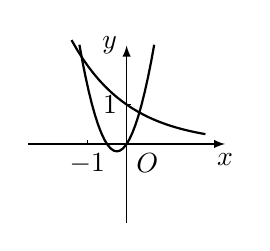
\begin{tikzpicture}[scale = 0.5, >=latex]
    \draw [->] (-2.5,0) -- (2.5,0) node [below] {$x$};
    \draw [->] (0,-2.) -- (0,2.5) node [left] {$y$};
    \draw (0,0) node [below right] {$O$};
    \draw (-1,0.1) -- (-1,0) node [below] {$-1$};
    \draw (0.1,1) -- (0,1) node [left] {$1$};
    \draw [domain = -1.2:0.7,thick] plot (\x,{3*\x * (\x+0.5)});
    \draw [domain = -1.4:2,thick] plot (\x,{(0.5)^\x}); 
\end{tikzpicture}
}{
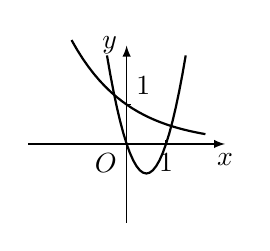
\begin{tikzpicture}[scale = 0.5, >=latex]
    \draw [->] (-2.5,0) -- (2.5,0) node [below] {$x$};
    \draw [->] (0,-2.) -- (0,2.5) node [left] {$y$};
    \draw (0,0) node [below left] {$O$};
    \draw (1,0.1) -- (1,0) node [below] {$1$};
    \draw (0.1,1) -- (0,1) node [above right] {$1$};
    \draw [domain = -0.5:1.5,thick] plot (\x,{3*\x*(\x-1)});
    \draw [domain = -1.4:2,thick] plot (\x,{(0.5)^\x}); 
\end{tikzpicture}
}{
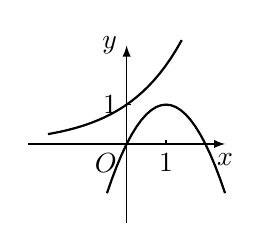
\begin{tikzpicture}[scale = 0.5, >=latex]
    \draw [->] (-2.5,0) -- (2.5,0) node [below] {$x$};
    \draw [->] (0,-2.) -- (0,2.5) node [left] {$y$};
    \draw (0,0) node [below left] {$O$};
    \draw (1,0.1) -- (1,0) node [below] {$1$};
    \draw (0.1,1) -- (0,1) node [left] {$1$};
    \draw [domain = -0.5:2.5,thick] plot ({\x},{-\x*(\x-2)});
    \draw [domain = -1.4:2,thick] plot ({-\x},{(0.5)^\x}); 
\end{tikzpicture}
}{
\begin{tikzpicture}[scale = 0.5, >=latex]
    \draw [->] (-2.5,0) -- (2.5,0) node [below] {$x$};
    \draw [->] (0,-2.) -- (0,2.5) node [left] {$y$};
    \draw (0,0) node [below right] {$O$};
    \draw (-1,0.1) -- (-1,0) node [below] {$-1$};
    \draw (0.1,1) -- (0,1) node [right] {$1$};
    \draw [domain = -2.5:0.5,thick] plot ({\x},{-\x*(\x+2)});
    \draw [domain = -1.4:2,thick] plot ({\x},{(0.5)^\x}); 
\end{tikzpicture}   
}
\item (000071)设$a$为常数且$0<a<1$, 若$y=(\log_a \dfrac 35)^x$在$\mathbf{R}$上是严格增函数, 求实数$a$的取值范围.
\item (000072)在同一平面直角坐标系中, 作出函数$y=(\dfrac 12)^x$及$y=x^{\frac 12}$的大致图像, 并求方程$(\dfrac 12)^x=x^{\frac 12}$的解的个数.
\item (000073)已知集合$A=\{y|y=(\dfrac 12)^x,\  x\in [-2, 0)\}$, 用列举法表示集合$B=\{y|y=\log_3x,\  x\in A\text{且}y\in \mathbf{Z}\}$.
\item (000074)$\log_23$是有理数吗? 请证明你的结论.
\item (000075)仅利用对数函数的单调性和计算器上的乘方功能来确定对数$\log_23$第二位小数的值.
\item (000076)求函数$y=\dfrac1{2-x}+\sqrt{x^2-1}$的定义域.
\item (000077)判断下列函数$y=f(x)$的奇偶性, 并说明理由:\\
(1) $f(x)=|\dfrac 12 x-3|+|\dfrac 12 x+3|$;\\
(2) $f(x)=x^3+\dfrac 2x$;\\
(3) $f(x)=x^2$, $x\in (k, 2)$(其中常数$k<2$).
\item (000078)已知$m$、$n$是常数, 而函数$y=(m-1)x^2+3x+(2-n)$为奇函数. 求$m$、$n$的值.
\item (000079)求函数$y=x+\dfrac 4x$的单调区间.
\item (000080)分别作出下列函数的大致图像, 并指出它们的单调区间:\\
(1) $y=|x^2-4x|$;\\
(2) $y=2|x|-3$.
\item (000081)已知二次函数$y=f(x)$, 其中$f(x)=ax^2-2ax+3-a \ (a>0)$. 比较$f(-1)$和$f(2)$的大小.
\item (000082)已知$k$是常数, 设$\alpha$、$\beta$是二次方程$x^2-2kx+k+20=0$的两个实根. 问: 当$k$为
何值时, $(\alpha+1)^2+(\beta+1)^2$取到最小值?
\item (000083)邮局规定: 当邮件质量不超过$100$g时, 每$20$g邮费$0.8$元, 且不足$20$g时按$20$g计算; 超过$100$g时, 超过$100$g的部分按每$100$g邮费$2$元计算, 且不足$100$g按$100$g
计算; 同时规定邮件总质量不得超过$2000$g. 请写出邮费关于邮件质量的函数表达式, 并计算$50$g和$500$g的邮件分别收多少邮费.
\item (000084)若函数$y=(a^2+4a-5)x^2-4(a-1)x+3$的图像都在$x$轴上方(不含$x$轴), 求实数$a$的取值范围.
\item (000085)已知$y=f(x)$是奇函数, 其定义域为$\mathbf{R}$; 而$y=g(x)$是偶函数, 其定义域为$D$. 判断函数$y=f(x)g(x)$的奇偶性, 并说明理由.
\item (000086)设函数$y=x^2+10x-a+3$, 当$x\in [-2, +\infty)$时, 其函数值恒大于等于零. 求实数$a$的取值范围.
\item (000087)已知函数$y=-x^2+2ax+1-a$, $x\in [0, 1]$的最大值为$2$. 求实数$a$的值.
\item (000088)设$f(x)=x^2+ax+1$. 若对任意给定的实数$x$, $f(2+x)=f(2-x)$恒成立, 求实数$a$的值.
\item (000089)已知$y=f(x)$是定义在$(-1, 1)$上的奇函数, 在区间$[0, 1)$上是严格减函数, 且$f(1-a)+f(1-a^2)<0$, 求实数$a$的取值范围.
\item (000090)已知$f(x)=2-x^2$及$g(x)=x$. 定义$h(x)$如下: 当$f(x)\ge g(x)$时, $h(x)=g(x)$; 而当$f(x)<g(x)$时, $h(x)=f(x)$. 求函数$y=h(x)$的最大值.
\item (000091)试讨论函数$y=\dfrac{x}{1-x^2}$的单调性.
\item (000092)作出函数$y=(x^2-1)^2-1$的大致图像, 写出它的单调区间, 并证明你的结论.
\item (000093)已知函数$y=f(x)$为偶函数, $y=g(x)$为奇函数, 且$f(x)+g(x)=x^2+2|x-1|+3$. 求$y=f(x)$及$y=g(x)$的表达式.
\item (000094)设函数$y=f(x)$, $x\in \mathbf{R}$的反函数是$y=f^{-1}(x)$.\\
(1) 如果$y=f(x)$是奇函数, 那么$y=f^{-1}(x)$的奇偶性如何?\\
(2) 如果$y=f(x)$在定义域上是严格增函数, 那么$y=f^{-1}(x)$的单调性如何?
\item (000095)选择题:\\
(1) 与$\sin(\theta -\dfrac\pi 2)$一定相等的是\bracket{20}.
\fourch{$\sin(\dfrac{3\pi}2-\theta)$}{$\cos(\theta -\dfrac{\pi}2)$}{$\cos (2\pi -\theta)$}{$\sin (\theta +\dfrac\pi 2)$}
(2) 当$0<\alpha<\dfrac\pi 4$时, 化简$\sqrt{1-\sin 2\alpha}$的结果是\bracket{20}.
\fourch{$\cos \alpha$}{$\sin \alpha-\cos \alpha$}{$\cos\alpha-\sin\alpha$}{$\sin\alpha+\cos\alpha$}
\item (000096)填空题:\\
(1) 若$\theta$为锐角, 则$\log_{\sin \theta} (1+\cot^2\theta)=$\blank{50};\\
(2) 若$-\dfrac\pi 2<\alpha<0$, 则点$(\cot \alpha, \cos \alpha)$必在第\blank{50}象限;\\
(3) 若$\sin (\pi -\alpha)=\dfrac 23$, $\alpha\in (\dfrac\pi 2, \pi)$, 则$\sin 2\alpha=$\blank{50}.
\item (000097)已知圆$O$上的一段圆弧长等于该圆的内接正方形的边长, 求这段圆弧所对的圆心角的弧度.
\item (000098)已知角$\alpha$的终边经过点$P(3a, 4a)$($a\ne 0$), 求$\sin \alpha$、$\cos \alpha$和$\tan \alpha$.
\item (000099)化简:\\
(1) $\dfrac{\sin (\theta -5\pi )}{\tan (3\pi -\theta )}\cdot \dfrac{\cot (\dfrac\pi 2-\theta )}{\tan (\theta -\dfrac{3\pi} 2)}\cdot \dfrac{\cos (8\pi -\theta )}{\sin(-\theta-4\pi)}$;\\
(2) $\sin (\theta -\dfrac\pi 4)+\cos (\theta +\dfrac\pi 4)$.
\item (000100)已知$\tan \alpha=3$, 求$\dfrac 1{\sin^2\alpha+2\sin \alpha\cos \alpha}$的值.
\item (000101)在$\triangle ABC$中, 已知$a=5$, $b=4$, $A=2B$. 求$\cos B$.
\item (000102)已知$\triangle ABC$的面积为$S$, 求证:\\
(1) $S=\dfrac{a^2\sin B\sin C}{2\sin (B+C)}$;\\
(2) $S=\dfrac{a^2}{2(\cot B+\cot C)}$.
\item (000103)(1) 已知$\sin \alpha=\dfrac{\sqrt 5}5$, $\sin \beta=\dfrac{\sqrt {10}}{10}$, 且$\alpha$及$\beta$都是锐角. 求$\alpha+\beta$的值;\\
(2) 在$\triangle ABC$中, 已知$\tan A$与$\tan B$是方程$x^2-6x+7=0$的两个根, 求$\tan C$.
\item (000104)证明: $(\sin \alpha+\sin \beta)^2+(\cos \alpha+\cos \beta)^2=4\cos^2\dfrac{\alpha-\beta}{2}$.
\item (000105)选择题:\\
(1) 若$0<x<\dfrac\pi 4$, 且$\lg (\sin x+\cos x)=\dfrac12(3\lg 2-\lg 5)$, 则$\cos x-\sin x$的值为\bracket{20}.
\fourch{$\dfrac{\sqrt{6}}3$}{$\dfrac{\sqrt{3}}2$}{$\dfrac{\sqrt{10}}5$}{$\dfrac{\sqrt{5}}4$}
(2) 下列命题中, 真命题为\bracket{20}.
\onech{若点$P(a, 2a)$($a\ne 0$)为角$\alpha$的终边上一点, 则$\sin \alpha=\dfrac{2\sqrt 5}5$}
{同时满足$\sin \alpha=\dfrac 12$, $\cos \alpha=\dfrac{\sqrt3}2$的角$\alpha$有且只有一个}
{如果角$\alpha$满足$-3\pi <\alpha<-\dfrac 52\pi$, 那么角$\alpha$是第二象限的角}
{$\tan x=-\sqrt 3$的解集为$\{x|x=k\pi -\dfrac\pi 3, \  k\in \mathbf{Z}\}$}
\item (000106)填空题:\\
(1) 在$\triangle ABC$中, 若$a^2+b^2+ab=c^2$, 则$C=$\blank{50};\\
(2) 若$\sin \theta =a$, $\cos \theta =-2a$, 且$\theta$为第四象限的角, 则实数$a=$\blank{50}.\\
\item (000107)已知$\sin \alpha=a\sin \beta$, $b\cos \alpha=a\cos \beta$, 且$\alpha$及$\beta$均为锐角, 求证: $\cos \alpha= \sqrt{\dfrac{a^2-1}{b^2-1}}$.
\item (000108)已知$0<\alpha<\dfrac\pi 2<\beta<\pi$, 且$\cos \beta=-\dfrac13$, $\sin (\alpha+\beta)=\dfrac79$, 求$\sin \alpha$的值.
\item (000109)已知$\pi <\alpha<\dfrac{3\pi} 2$, $\pi <\beta<\dfrac{3\pi} 2$, 且$\sin \alpha=-\dfrac{\sqrt 5}5$, $\cos \beta=-\dfrac{\sqrt{10}}{10}$. 求$\alpha-\beta$的值.
\item (000110)已知$(1+\tan \alpha)(1+\tan \beta)=2$, 且$\alpha$及$\beta$都是锐角. 求证: $\alpha+\beta=\dfrac{\pi}{4}$.
\item (000111)已知$\alpha$是第二象限的角, 且$\sin \alpha=\dfrac{\sqrt {15}}4$. 求$\dfrac{\sin (\alpha+\dfrac{\pi}{4})}{1+\sin 2\alpha+\cos 2\alpha}$的值.
\item (000112)证明:\\
(1) $\dfrac{2(1+\sin 2\alpha)}{1+\sin 2\alpha+\cos 2\alpha}=1+\tan \alpha$;\\
(2) $2\sin \alpha+\sin 2\alpha=\dfrac{2\sin^3\alpha}{1-\cos \alpha}$.
\item (000113)根据下列条件, 分别判断三角形$ABC$的形状:\\
(1) $\sin C+\sin (B-A)=\sin 2A$;\\
(2) $\dfrac{\tan A}{\tan B}=\dfrac{a^2}{b^2}$.
\item (000114)在$\triangle ABC$中, 求证: $\tan \dfrac A2\tan \dfrac B2+\tan \dfrac B2\tan\dfrac C2+\tan\dfrac C2\tan\dfrac A2=1$.
\item (000115)(1) 完成下表($\theta$为弧度数):
\begin{center}
\begin{tabular}{|c|p{.15\textwidth}<{\centering}|p{.15\textwidth}<{\centering}|p{.15\textwidth}<{\centering}|p{.15\textwidth}<{\centering}|p{.15\textwidth}<{\centering}|}
    \hline
    $\theta$ & $1$ & $0.5$ & $0.1$ & $0.01$ & $0.001$\\ \hline
    $\sin\theta$ & & & & &\\ \hline
    $\dfrac{\sin\theta}{\theta}$ & & & & &\\ \hline
\end{tabular}
\end{center}
(2) 观察上表中的数据, 你能发现什么规律?\\
(3) 已知$0<\theta <\dfrac \pi 2$, 利用图形面积公式证明$\sin \theta <\theta <\tan \theta$, 并应用该公式说明(2)中猜想的合理性.
\item (000116)在$\triangle ABC$中, 已知$A=30^\circ$, $b=18$. 分别根据下列条件求$B$:\\
(1) \textcircled{1} $a=6$, \textcircled{2} $a=9$, \textcircled{3} $a=13$, \textcircled{4} $a=18$, \textcircled{5} $a=22$;\\
(2) 根据上述计算结果, 讨论使$B$有一解、两解或无解时$a$的取值情况.
\item (000117)(1) 根据$\cos 54^\circ=\sin 36^\circ$和三倍角公式, 求$\sin 18^\circ$的值;\\
(2) 你还能使用其他方法求$\sin 18^\circ$的值吗? 若能, 请给出你的求法.
\item (000118)如图, 要在$A$和$D$两地之间修建一条笔直的隧道, 现在从$B$地和$C$地测量得到: $\angle DBC=24.2^\circ$, $\angle DCB=35.4^\circ$, $\angle DBA=31.6^\circ$, $\angle DCA=17.5^\circ$. 试求$\angle DAB$以确定隧道$AD$的方向(结果精确到$0.1^\circ$).
\begin{center}
    \begin{tikzpicture}
        \draw (0,0) node [below] {$D$} coordinate (D) (0,1.5) node [above] {$C$} coordinate (C) (-0.8287,-1.12831) node [below left] {$A$} coordinate (A) (1.82829,-1.07265) node [below right] {$B$} coordinate (B);
        \draw [thick] (A) -- (B) -- (C) -- cycle;
        \draw [thick] (D) -- (A) (D) -- (B) (D) -- (C);
    \end{tikzpicture}
\end{center}
\item (000119)求下列函数的最小正周期:\\
(1) $y=\sin \dfrac x2$;\\
(2) $y=2\cos (3x-\dfrac \pi 4)$.
\item (000120)判断下列函数的奇偶性, 并说明理由:\\
(1) $y=\sin |2x|$;\\
(2) $y=\tan 5x$;\\
(3) $y= \dfrac1 {\cos x}$;\\
(4) $y=\sin (x+\dfrac\pi 6)$.
\item (000121)已知$2\sin (2x)=\sqrt 3, \ x\in (-\dfrac \pi 4, \dfrac\pi 4)$. 求$x$的值.
\item (000122)求下列函数的单调区间:\\
(1) $y=-\sin 2x$;\\
(2) $y=2\sin (x+\dfrac\pi 3)$;\\
(3) $y=\cos (\dfrac x2-\dfrac \pi 4)$;\\
(4) $y=2\tan (2x+\dfrac \pi 4)$.
\item (000123)作出函数$y=2\sin (2x+\dfrac \pi 3)$的大致图像.
\item (000124)已知函数$y=A\sin (\omega x+\varphi) \ (A>0, \ \omega>0)$的振幅是$3$, 最小正周期是$\dfrac{2\pi} 3$, 初始相位是$\dfrac\pi 6$. 求这个函数的表达式.
\item (000125)求下列函数的最大值和最小值, 并求出取得最大值和最小值时所有$x$的值:\\
(1) $y=\cos^2x+\cos x-2$;\\
(2) $y=\sin 2x, \ x\in [ -\dfrac{2\pi} 3, \dfrac \pi 3]$;\\
(3) $y=\sin^22x-2\sin 2x$;\\
(4) $y=\cos (x-\dfrac\pi 6),\  x\in  [-\dfrac\pi 6, \dfrac\pi 4]$.
\item (000126)某实验室一天的温度$y$(单位:$^\circ\text{C}$)随时间$t$(单位:$\text{h}$)的变化近似满足函数关系$y=10-\sqrt 3\cos\dfrac \pi {12}t-\sin \dfrac\pi {12} t, \ t\in [0, 24)$.\\
(1) 求实验室一天中的最大温差;\\
(2) 若要求实验室温度不高于$11^\circ\text{C}$, 则在哪段时间实验室需要降温?
\item (000127)求函数$y=\sin (2x-\dfrac \pi 4)-2\sqrt 2\sin^2x$的最小正周期.
\item (000128)在$(0, 2\pi )$内, 求使$\sin x>\cos x$成立的$x$的取值范围.
\item (000129)求下列函数的最大值, 并求出取得最大值时所有$x$的值:\\
(1) $y=2\sin^2x+\sin 2x-1$;\\
(2) $y=1-\sin x-2\cos^2x, \  x\in  [\dfrac \pi 3, \dfrac{4\pi} 3]$.
\item (000130)若函数$y=2\sin \omega x$(其中常数$\omega$是小于$1$的正数)在区间$[0, \dfrac\pi 3]$上的最大值是$\sqrt 2$, 求$\omega$的值.
\item (000131)如图, 摩天轮上一点$P$距离地面的高度$y$关于时间$t$的函数表达式为$y=A\sin (\omega t+\varphi)+b$, $\varphi\in [-\pi , \pi]$. 已知摩天轮
的半径为$50\text{m}$, 其中心点$O$距地面$60\text{m}$, 摩天轮以每$30$分钟转一圈的方式做匀速转动, 而点$P$的起始位置在摩天轮的最低
点处.
\begin{center}
    \begin{tikzpicture}[>=latex,scale = 0.4]
        \draw [thick] (0,0) circle (0.3) (0,0) circle (5);
        \foreach \i in {0,30,...,330}{\draw [thick] (\i:0.3) -- (\i:5);};
        \draw [thick] (-80:0.3) -- (-80:5.5) coordinate (R) (-100:0.3) -- (-100:5.5) coordinate (L) (L) -- (R);
        \draw [thick] (L) --++ (-135:0.3) --++ (-4,0) -- (-5.5,-6) (R) --++ (-45:0.3) --++ (4,0) -- (5.5,-6); 
        \draw [thick] (-6,-6) -- (6,-6);
        \draw (-6.2,-6) -- (-7.5,-6) (-5.2,0) -- (-7.5,0) (0,-5) -- (-6.5,-5);
        \draw [->] (-5.6,-2) -- (-5.6,0);
        \draw [->] (-5.6,-3) -- (-5.6,-5);
        \draw (-5.6,-2.5) node {$50$};
        \draw [->] (-7,-2.5) -- (-7,0);
        \draw [->] (-7,-3.5) -- (-7,-6);
        \draw (-7,-3) node {$60$};
        \draw (225:2) node {$O$};
        \draw (-30:5) node [below right] {$P$};
    \end{tikzpicture}
\end{center}
(1) 根据条件具体写出$y$($\text{m}$)关于$t$($\text{min}$)的函数表达式;\\
(2) 在摩天轮转动的一圈内, 点$P$有多长时间距离地面超过$85\text{m}$?
\item (000132)说明: 用上一章6.3节给出的记号$\arcsin$与$\arccos$(见必修第二册教材第45页), 可以定义函数$y=\arcsin x \ (x\in [0, 1])$与$y=\arccos x \ (x\in [0, 1])$.\\
验证:\\
(1) 函数$y=\sin x\ (x\in [0, \dfrac\pi 2])$与函数$y=\arcsin x \ (x\in [0, 1])$互为反函数;\\
(2) 函数$y=\cos x \ (x\in [0, \dfrac \pi 2])$与函数$y=\arccos x\ (x\in [0, 1])$互为反函数.
\item (000133)把上题的记号略作推广: 对实数$x\in [-1, 1]$, 若实数$y\in [-\dfrac \pi 2, \dfrac\pi 2]$使得$\sin y=x$, 则记$y=\arcsin x$; 类似地, 对实数$x\in [-1, 1]$, 若实数$y\in [0, \pi]$使得$\cos y=x$, 则记$y=\arccos x$. 说明: 经过推广的记号$\arcsin$与$\arccos$, 定义了函数$y=\arcsin x \ (x\in [-1, 1])$与$y=\arccos x \ (x\in [-1, 1])$.\\
验证:
(1) 函数$y=\sin x \ (x\in  [-\dfrac\pi 2, \dfrac\pi 2])$与函数$y=\arcsin x \ (x\in [-1, 1])$互为反函数;\\
(2) 函数$y=\cos x\ (x\in [0, \pi])$与函数$y=\arccos x \ (x\in [-1, 1])$互为反函数.
\item (000134)对$y=\tan x$与$y=\arctan x$做类似的工作.
\item (000135)定义在区间$(0, \dfrac\pi 2)$上的函数$y=6\cos x$的图像与$y=5\tan x$的图像的交点为$P$, 过点$P$作垂直于$x$轴的垂线$PP_1$, 其垂足为$P_1$. 设直线$PP_1$与$y=\sin x$的图像交于点$P_2$, 求线段$P_1P_2$的长.
\item (000136)已知定义在$\mathbf{R}$上的偶函数$y=f(x)$的最小正周期为$2$, 当$0\le x\le 1$时, $f(x)=x$.\\
(1) 求当$5\le x\le 6$时函数$y=f(x)$的表达式;\\
(2) 若函数$y=kx,\ x\in \mathbf{R}$与函数$y=f(x)$的图像恰有$7$个不同的交点, 求$k$的值.
\item (000137)如图, 有一块边长为$3\text{m}$的正方形铁皮$ABCD$, 其中阴影部分$ATN$是一个半径为$2\text{m}$的扇形. 设这个扇形已经腐蚀不能
使用, 但其余部分均完好. 工人师傅想在未被腐蚀的部分截下一块其边落在$BC$与$CD$上的矩形铁皮$PQCR$, 使点$P$在弧$TN$上. 设$\angle TAP=\theta$, 矩形$PQCR$的面积为$S\text{m}^2$.
\begin{center}
    \begin{tikzpicture}
        \begin{scope}[even odd rule]
            \clip (0,0) rectangle (3,3) (0.55,0.15) circle (0.15);
            \fill [gray!30] (0,0) -- (2,0) arc (0:90:2) -- cycle;
        \end{scope}

        \draw [thick] (0,0) node [below left] {$O$} -- (3,0) node [below right] {$B$} -- (3,3) node [above right] {$C$} -- (0,3) node [above left] {$D$} -- cycle;
        \draw [thick] (0,0) -- (40:2) node [above right] {$P$} -- (3,{2*sin(40)}) node [right] {$Q$} (40:2) -- ({2*cos(40)},3) node [above] {$R$};
        \draw [thick] (0,0) -- (2,0) node [below] {$T$} arc (0:90:2) node [left] {$N$} -- cycle;
        \draw (0.4,0) arc (0:40:0.4) (0.55,0.15) node {$\theta$};
    \end{tikzpicture}
\end{center}
(1) 求$S$关于$\theta$的函数表达式;\\
(2) 求$S$的最大值及$S$取得最大值时$\theta$的值.
\item (000138)如图, 在边长为$1$的小正方形组成的网格上, 求:
\begin{center}
    \begin{tikzpicture}[>=latex,scale = 0.5]
        \foreach \i in {0,1,...,4} {\draw [dashed, very thin] (0,\i) -- (6,\i);};
        \foreach \i in {0,1,...,6} {\draw [dashed, very thin] (\i,0) -- (\i,4);};
        \draw [thick,->] (0,1) node [left] {$A$} -- (3,4) node [above] {$B$};
        \draw [thick,->] (1,0) node [below] {$C$} -- (6,1) node [right] {$D$};
        \draw [thick, ->] (4,4) node [above] {$E$} -- (6,2) node [right] {$F$};       
    \end{tikzpicture}
\end{center}
(1) $|\overrightarrow{AB}|$;\\
(2) $|\overrightarrow{CD}|$;\\
(3) $|\overrightarrow{EF}|$.
\item (000139)已知$\overrightarrow a$、$\overrightarrow b$均为非零向量, 写出$|\overrightarrow a+\overrightarrow b|=|\overrightarrow a|+|\overrightarrow b|$成立的充要条件.
\item (000140)已知$\overrightarrow a$、$\overrightarrow b$为非零向量, 且$\overrightarrow a$、$\overrightarrow b$、$5\overrightarrow a-4\overrightarrow b$在同一起点上. 求证: 它们的终点在同一条直线上.
\item (000141)在矩形$ABCD$中, 边$AB$、$AD$的长分别为$2$、$1$, 若$M$、$N$分别是边$BC$、$CD$上的点, 且满足$\dfrac{|\overrightarrow{BM}|}{|\overrightarrow{BC}|}=\dfrac{|\overrightarrow{CN}|}{|\overrightarrow{CD}|}$, 则$\overrightarrow{AM}\cdot \overrightarrow{AN}$的取值范围是\blank{50}.
\item (000142)已知两个向量$\overrightarrow {e_1}$、$\overrightarrow {e_2}$满足$|\overrightarrow {e_1}|=2$, $|\overrightarrow {e_2}|=1$, $\langle \overrightarrow {e_1}, \overrightarrow {e_2}\rangle=60^\circ$, 且向量$2\lambda \overrightarrow {e_1}+7\overrightarrow {e_2}$与向量$\overrightarrow {e_1}+\lambda \overrightarrow {e_2}$的夹角为钝角. 求实数$\lambda$的取值范围.
\item (000143)已知向量$\overrightarrow a=(1, 0)$, $\overrightarrow b=(2, 1)$.\\
(1) 求$|\overrightarrow a+3\overrightarrow b|$;\\
(2) 当$k$为何实数时, $k\overrightarrow a-\overrightarrow b$与$\overrightarrow a+3\overrightarrow b$平行? 平行时它们是同向还是反向?
\item (000144)已知在平面直角坐标系中, $O$为原点, 点$A(4, -3)$, $B(-5, 12)$.\\
(1) 求向量$\overrightarrow{AB}$的坐标及$|\overrightarrow{AB}|$;\\
(2) 已知向量$\overrightarrow{OC}=2\overrightarrow{OA}+\overrightarrow{OB}$, $\overrightarrow{OD}=\overrightarrow{OA}-3\overrightarrow{OB}$, 求$\overrightarrow{OC}$及$\overrightarrow{OD}$的坐标;\\
(3) 求$\overrightarrow{OA}\cdot\overrightarrow{OB}$.
\item (000145)已知向量$\overrightarrow a=(3, -2)$, $\overrightarrow b=(-2, 1)$, $\overrightarrow c=(7, -4)$, 求$\lambda,\mu$, 使得$\overrightarrow c=\lambda \overrightarrow a+\mu \overrightarrow b$.
\item (000146)已知点$M(3, -2)$、$N(-5, -1)$, 且$\overrightarrow{MP}=\dfrac 13\overrightarrow{MN}$. 求点$P$的坐标.
\item (000147)在等腰三角形$ABC$中, 已知$D$为底边$BC$的中点. 求证: $AD\perp BC$.
\item (000148)如图, 在四边形$ABCD$中, $G$为对角线$AC$与$BD$中点连线$MN$的中点, $P$为平面上任意给定的一点. 求证: $4\overrightarrow{PG}=\overrightarrow{PA}+\overrightarrow{PB}+\overrightarrow{PC}+\overrightarrow{PD}$.
\item (000149)在四边形$ABCD$中, 向量$\overrightarrow{AB}=\overrightarrow i+2\overrightarrow j$, $\overrightarrow{BC}=-4\overrightarrow i-\overrightarrow j$, $\overrightarrow{CD}=-5\overrightarrow i-3\overrightarrow j$. 求证: $ABCD$为梯形.
\begin{center}
    \begin{tikzpicture}
        \draw [thick] (0,0) node [below left] {$B$} coordinate (B) -- (2,0) node [below right] {$C$} coordinate (C) -- (2.4,2.5) node [above right] {$D$} coordinate (D) -- (-0.1,1.5) node [above left] {$A$} coordinate (A) -- cycle;
        \draw [thick] (A) -- (C) (B) -- (D);
        \filldraw ($(B)!0.5!(D)$) circle (0.03) node [above] {$M$} coordinate (M);
        \filldraw ($(A)!0.5!(C)$) circle (0.03) node [below] {$N$} coordinate (N);
        \filldraw ($(M)!0.5!(N)$) circle (0.03) node [right] {$G$} coordinate (G);
        \filldraw (3,1) circle (0.03) node [right] {$P$};
        \draw [thick] (M) -- (N);
    \end{tikzpicture}
\end{center}
\item (000150)已知$\overrightarrow a$、$\overrightarrow b$、$\overrightarrow c$均为非零向量, 其中的任意两个向量都不平行, 且$\overrightarrow a+\overrightarrow b$与$\overrightarrow c$是平行向量, $\overrightarrow a+\overrightarrow c$与$\overrightarrow b$是平行向量. 求证: $\overrightarrow b+\overrightarrow c$与$\overrightarrow a$是平行向量.
\item (000151)如图, 点$A$、$M$、$B$在同一条直线上, 点$O$不在该直线上, 且$\overrightarrow{AM}=\dfrac 13 \overrightarrow{AB}$. 设
$\overrightarrow{OA}=\overrightarrow a$, $\overrightarrow{OB}=\overrightarrow b$, $\overrightarrow{OM}=\overrightarrow c$, 试用向量$\overrightarrow a$、$\overrightarrow b$表示$\overrightarrow c$.
\begin{center}
    \begin{tikzpicture}[>=latex]
        \draw [thick] (-0.5,0) -- (3.5,0);
        \draw [->,thick] (1.5,-1.5) node [below] {$O$}-- (0,0) node [above] {$A$};
        \draw [->,thick] (1.5,-1.5) -- (3,0);
        \draw [->,thick] (1.5,-1.5) -- (1,0);
        \draw [->,thick] (0,0) -- (1,0) node [above] {$M$};
        \draw [->,thick] (1,0) -- (3,0) node [above] {$B$};
    \end{tikzpicture}
\end{center}
\item (000152)设平面上有两个向量$\overrightarrow a=(\cos \alpha, \sin \alpha)  (0^\circ\le \alpha<360^\circ)$, $\overrightarrow b=(-\dfrac 12, \dfrac{\sqrt 3}2)$.\\
(1) 求证: 向量$\overrightarrow a+\overrightarrow b$与$\overrightarrow a-\overrightarrow b$垂直;\\
(2) 当向量$\sqrt 3\overrightarrow a+\overrightarrow b$与$\overrightarrow a-\sqrt 3\overrightarrow b$的模相等时, 求$\alpha$的大小.
\item (000153)如图, 在矩形$ABCD$中, $AB=\sqrt 2$, $BC=2$, $E$为$BC$的中点, 点$F$在边$CD$上且$\overrightarrow{AB}\cdot \overrightarrow{AF}=\sqrt{2}$. 求$\overrightarrow{AE}\cdot \overrightarrow{BF}$的值.
\begin{center}
    \begin{tikzpicture}[>=latex,thick,scale = 1.3]
        \draw (0,0) node [below left] {$A$} rectangle ({sqrt(2)},2) node [above right] {$C$};
        \draw [->,thick] (0,0) -- ({sqrt(2)},1) node [right] {$E$};
        \draw [->] (0,0) -- (1,2) node [above] {$F$};
        \draw [->] ({sqrt(2)},0) node [below right] {$B$} -- (1,2);
        \draw (0,2) node [above left] {$D$};
    \end{tikzpicture}
\end{center}
\item (000154)已知等边三角形$ABC$的边长为$1$, $\overrightarrow{BC}=\overrightarrow a$, $\overrightarrow{CA}=\overrightarrow b$, $\overrightarrow{AB}=\overrightarrow c$. 求$\overrightarrow a\cdot \overrightarrow b+\overrightarrow b\cdot \overrightarrow c+\overrightarrow c\cdot \overrightarrow a$.
\item (000155)已知向量$\overrightarrow{OA}=(k, 12)$, $\overrightarrow{OB}=(4, 5)$, $\overrightarrow{OC}=(-k, 10)$, 且$A$、$B$、$C$三点共线. 求实数$k$的值.
\item (000156)已知向量$\overrightarrow{OA}=(1, 7)$, $\overrightarrow{OB}=(5, 1)$, $\overrightarrow{OP}=(2, 1)$, $K$为直线$OP$上的一个动点, 当$\overrightarrow{KA}\cdot\overrightarrow{KB}$取最小值时, 求向量$\overrightarrow{OK}$的坐标.
\item (000157)如图, 在正方形$ABCD$中, $P$是对角线$AC$上一点, $PE$垂直$AB$于点$E$, $PF$垂直$BC$于点$F$. 求证: $PD\perp EF$.
\begin{center}
    \begin{tikzpicture}[thick]
        \draw (0,0) node [below left] {$A$} rectangle (2,2) node [above right] {$C$};
        \draw (0,2) node [above left] {$D$} -- (1.5,1.5) node [above] {$P$};
        \draw (1.5,1.5) -- (1.5,0) node [below] {$E$} -- (2,1.5) node [right] {$F$} -- cycle;
        \draw (2,0) node [below right] {$B$};
        \draw (0,0) -- (2,2);
    \end{tikzpicture}
\end{center}
\item (000158)证明: 三角形的三条高相交于一点.
\item (000159)如图, 甲、乙分处河的两岸, 欲拉船$M$逆流而上, 需在正前方有$3000\text{N}$的力. 已知甲所用的力$\overrightarrow{f_1}$的大小为$2000\text{N}$, 且与$M$的前进方向的夹角为$\dfrac\pi 6$, 求乙所用的力$\overrightarrow{f_2}$.
\begin{center}
    \begin{tikzpicture}[thick,>=latex,scale = 1.5]
        \fill [fill = gray!20] (0,0.3) -- (0,1.4) -- (3,1.7) -- (3,0.6) -- cycle;
        \draw (0,1.4) -- (3,1.7) (0,0.3) -- (3,0.6);
        \draw [->] (0.6,1) node [below left] {$M$} -- (3,1);
        \draw [dashed,thin] (0,1) -- (0.6,1);
        \draw [->] (0.6,1) --++ (30:1.6) node [above right] {$\overrightarrow{f_1}$};
        \draw [->] (0.6,1) --++ ({2.4-1.6*cos(30)},{-1.6*sin(30)}) node [below right] {$\overrightarrow{f_2}$};
        \draw (2.2,1) node [above] {前进方向};
    \end{tikzpicture}
\end{center}
\item (000160)在$\triangle ABC$中, $AB=AC=5$, $BC=6$, $M$是边$AC$上靠近$A$的一个三等分点. 问: 在线段$BM$上是否存在点$P$, 使得$PC\perp BM$?
\item (000161)在$\triangle ABC$中, 已知点$O$、$G$、$H$分别是三角形的外心、重心和垂心. 求证: $O$、$G$、$H$三点共线(此直线称为欧拉线).
\item (000162)选择题:\\
(1) 虚数的平方一定是\bracket{20}.
\fourch{正实数}{负实数}{虚数}{虚数或负实数}
(2) 如果复平面上的向量$\overrightarrow{AB}$所对应的复数是$-3+2\mathrm{i}$, 那么向量$\overrightarrow{BA}$所对应的复数是\bracket{20}.
\fourch{$3-2\mathrm{i}$}{$3+2\mathrm{i}$}{$-3+2\mathrm{i}$}{$-3-2\mathrm{i}$}
\item (000163)填空题:\\
(1) 设$z=11-60\mathrm{i}$, 则$\mathrm{Re}z=$\blank{50}; $\mathrm{Im}z=$\blank{50}; $|z|=$\blank{50}; $\overline{z}=$\blank{50}.\\
(2) 下列三个命题中, 真命题是\blank{50}.\\
\textcircled{1} 在复平面上, 表示实数的点都在实轴上, 表示虚数的点都在虚轴上;\\
\textcircled{2} 任何一个表示虚数的点一定在某一个象限内;\\
\textcircled{3} 复数的模表示该复数在复平面上所对应的点到原点的距离.
\item (000164)已知复数$z=(a^2-2a-3)+(a^2-4a+3)\mathrm{i}$, 其中$a$是实数.\\
(1) 若$z\in \mathbf{R}$, 求$a$的值;\\
(2) 若$z$在复平面上所对应的点位于第一象限, 求$a$的取值范围.
\item (000165)已知复数$z_1=(a^2-a-6)+(1-2a)\mathrm{i}$, $z_2=(a-3)+(a^2-2a+2)\mathrm{i}$, 其中$a\in \mathbf{R}$.
若$\overline{z_1}=z_2$, 求$a$的值.
\item (000166)计算:\\
(1) $(4+\mathrm{i})(3+2\mathrm{i})$;\\
(2) $(\sqrt 2+\sqrt 3\mathrm{i})(\sqrt 2-\sqrt 3\mathrm{i})(-\sqrt 3+\sqrt 2\mathrm{i})(-\sqrt 3-\sqrt 2\mathrm{i})$;\\
(3) $\dfrac{-3+29\mathrm{i}}{1+2\mathrm{i}}$;\\
(4) $\dfrac{(1+\mathrm{i})^4}{1+2\mathrm{i}}+\dfrac{(1-\mathrm{i})^4}{1-2\mathrm{i}}$;\\
(5) $[(\sqrt 3+1)+(\sqrt 3-1)\mathrm{i}]^2$.
\item (000167)已知复数$z=\dfrac{(-3-\mathrm{\mathrm{i}})^2(2-\mathrm{\mathrm{i}})}{(1+2\mathrm{i})^3}$, 求$|z|$.
\item (000168)在复数范围内解下列方程:\\
(1) $x^2-4x+8=0$;\\
(2) $3x^2+2x-3=0$.
\item (000169)选择题:\\
(1) 设$z_1$、$z_2\in \mathbf{C}$, 则``$|z_1|=|z_2|$''是``$z_1=z_2$''的\bracket{20}.
\twoch{充分非必要条件}{必要非充分条件}{充要条件}{既非充分也非必要条件}\\
(2)设复数$z=a+b\mathrm{i}$($a,b\in \mathbf{R}$), 则$z^2$是纯虚数的充要条件是\bracket{20}.
\fourch{$a^2=b^2$}{$a^2+b^2=0$}{$|a|=|b|\ne 0$}{$ab\ne 0$}
\item (000170)若复数$z$满足$z+\overline{z}=2$, $(z-\overline{z})\mathrm{i}=2$, 求$|z|$.
\item (000171)若复数$z_1$和复数$z_2$满足$z_1z_2=3-4\mathrm{i}$, $|z_1|=2$, 求$|z_2|$.
\item (000172)若$x_1$和$x_2$是方程$x^2-5x+8=0$的两个根, 求$|x_1|+|x_2|$的值.
\item (000173)若复数$z_1$和复数$z_2$满足$|z_1|=3$, $|z_2|=4$, $|z_1+z_2|=5$, 求$|z_1-z_2|$.
\item (000174)已知复数$z_1$和复数$z_2$满足$z_1+z_2=3-5\mathrm{i}$, $\overline{z_1}-\overline{z_2}=-2+3\mathrm{i}$. 求$z_1^2-z_2^2$.
\item (000175)如图, 在长方体$ABCD-A_1B_1C_1D_1$中, $E$为$A_1B_1$的中点, $AB=BB_1=2$, $AC=2\sqrt 5$. 求异面直线$BE$与$AC$所成角的
大小. 
\begin{center}
    \begin{tikzpicture}[thick]
        \draw (0,0) node [below left] {$A$} coordinate (A) --++ (2,0) node [below right] {$B$} coordinate (B) --++ (45:{2*sqrt(5)/2}) node [right] {$C$} coordinate (C)
        --++ (0,2) node [above right] {$C_1$} coordinate (C1)
        --++ (-2,0) node [above left] {$D_1$} coordinate (D1) --++ (225:{2*sqrt(5)/2}) node [left] {$A_1$} coordinate (A1) -- cycle;
        \draw (A) ++ (2,2) node [right] {$B_1$} coordinate (B1) -- (B) (B1) --++ (45:{2*sqrt(5)/2}) (B1) --++ (-2,0);
        \draw [dashed] (A) --++ (45:{2*sqrt(5)/2}) node [left] {$D$} coordinate (D) --++ (2,0) (D) --++ (0,2);
        \draw ($(A1)!0.5!(B1)$) node [above] {$E$} -- (B);
        \draw [dashed] (A) -- (C);
    \end{tikzpicture}
\end{center}
\item (000176)如图, 设$P$为矩形$ABCD$所在平面外的一点, 矩形对角线的交点为$O$, $M$为$PB$的中点. 判断下列结论是否正确, 并说
明理由:\\
\begin{center}
    \begin{tikzpicture}[thick]
        \draw (0,0) node [below left] {$A$} coordinate (A) -- (3,0) node [below right] {$B$} coordinate (B)--++ (45:1.5) node [above right] {$C$} coordinate (C);
        \draw [dashed] (C) --++ (-3,0) node [above right] {$D$} coordinate (D) -- (A);
        \draw [dashed] (A) -- (C) (B) -- (D);
        \draw ($(A)!0.5!(C)$) node [below] {$O$} coordinate (O) ++ (0,3) node [above] {$P$} coordinate (P);
        \draw (P) -- (A) (P) -- (B) (P) -- (C);
        \draw ($(P)!0.5!(B)$) node [above right] {$M$} coordinate (M);
        \draw [dashed] (M) -- (O) (P) -- (D);
    \end{tikzpicture}
\end{center}
(1) $OM\parallel PD$;\\
(2) $OM\parallel\text{平面}PCD$;\\
(3) $OM\parallel\text{平面}PDA$;\\
(4) $OM\parallel\text{平面}PBA$;\\
(5) $OM\parallel\text{平面}PBC$.
\item (000177)如图, 正方体的棱长是$a$, 点$E$、$F$分别是两条棱的中点.
\begin{center}
    \begin{tikzpicture}[thick]
        \path (0,0) node [below left] {$A$} coordinate (A) --++ (2.5,0) node [below right] {$B$} coordinate (B) --++ (45:{2.5/2}) node [right] {$C$} coordinate (C)
        --++ (0,2.5) node [above right] {$C_1$} coordinate (C1)
        --++ (-2.5,0) node [above left] {$D_1$} coordinate (D1) --++ (225:{2.5/2}) node [left] {$A_1$} coordinate (A1) -- cycle;
        \path (A) ++ (2.5,2.5) node [right] {$B_1$} coordinate (B1) -- (B) (B1) --++ (45:{2.5/2}) (B1) --++ (-2.5,0);
        \path [dashed] (A) --++ (45:{2.5/2}) node [left] {$D$} coordinate (D) --++ (2.5,0) (D) --++ (0,2.5);
        \draw ($(A1)!0.5!(D1)$) node [above left] {$E$} coordinate (E) ($(A1)!0.5!(B1)$) node [above] {$F$} coordinate (F);
        \fill [gray!30] (B) -- (D) -- (E) -- (F);
        \draw (B) -- (F) -- (E);
        \draw [dashed] (B) -- (D) -- (E) (D) -- (C) (D) -- (A) (D) -- (D1);
        \draw (A) -- (B) -- (C) -- (C1) -- (D1) -- (A1) -- (A) (B1) -- (A1) (B1) -- (C1) (B1) -- (B);
    \end{tikzpicture}
\end{center}
(1) 求证: 四边形$BDEF$(图中阴影部分)是一个梯形;\\
(2) 求四边形$BDEF$的面积.
\item (000178)判断下列命题的真假, 并说明理由:\\
(1) 若直线$l$与平面$M$斜交, 则$M$内不存在与$l$垂直的直线;\\
(2) 若直线$l\perp\text{平面}M$, 则$M$内不存在与$l$不垂直的直线;\\
(3) 若直线$l$与平面$M$斜交, 则$M$内不存在与$l$平行的直线;\\
(4) 若直线$l\parallel\text{平面}M$, 则$M$内不存在与$l$不平行的直线.
\item (000179)如果不在平面上的一条直线上有两点到这个平面的距离相等, 那么这条直线和这个平面有什么位置关系? 画示意图表示.
\item (000180)如图, 直线$AA'$、$BB'$、$CC'$相交于点$O$, 且$AO=A'O$, $BO=B'O$, $CO=C'O$. 求证: $\text{平面}ABC\parallel \text{平面}A'B'C'$.
\begin{center}
    \begin{tikzpicture}[thick]
        \draw (0,0) node [below left] {$A$} coordinate (A);
        \draw (2.5,-0.5) node [below right] {$B$} coordinate (B);
        \draw (1.5,0.5) node [below] {$C$} coordinate (C);
        \draw (1,1.5) node [left] {$O$} coordinate (O);
        \draw (A) -- (B) -- (O) -- cycle;
        \draw [dashed] (A) -- (C) -- (B) (C) -- (O);
        \draw ($(O)!-1!(C)$) node [above] {$C'$} coordinate (C1);
        \draw ($(O)!-1!(A)$) node [right] {$A'$} coordinate (A1);
        \draw ($(O)!-1!(B)$) node [left] {$B'$} coordinate (B1);
        \draw (O) -- (A1) -- (B1) -- (C1) -- (O) (A1) -- (C1) (B1) -- (O);
    \end{tikzpicture}
\end{center}
\item (000181)已知直线$l\perp\text{平面}\alpha$, 直线$m\subset\text{平面}\beta$, 判断下列命题的真假, 并说明理由:\\
(1) 若$\alpha\parallel \beta$, 则$l\perp m$;\\
(2) 若$\alpha\perp \beta$, 则$l\parallel m$;\\
(3) 若$l\parallel m$, 则$\alpha\perp \beta$;\\
(4) 若$l\perp m$, 则$\alpha\parallel \beta$.
\item (000182)如图, 已知线段$AB$垂直于三角形$BCD$所在的平面, 且$AB=BC=CD=1$, $\angle BCD=90^\circ$. $BE\perp AD$, $E$为垂足, $F$为$AC$的中点. 求$EF$的长.
\begin{center}
    \begin{tikzpicture}[thick,scale = 2]
        \draw (0,0) node [left] {$B$} coordinate (B) -- (0,1) node [above left] {$A$} coordinate (A);
        \draw ({sqrt(2)/2},0) ++ (-45:{sqrt(2)/4}) coordinate (C) node [below] {$C$};
        \draw ({sqrt(2)},0) node [right] {$D$} coordinate (D) -- (C) -- (B) (A) -- (C) (A) -- (D);
        \draw ($(A)!{1/3}!(D)$) node [above] {$E$} coordinate (E) -- ($(A)!0.5!(C)$) node [right] {$F$} coordinate (F);
        \draw (E) -- (F) -- (B);
        \draw [dashed] (E) -- (B) -- (D);
    \end{tikzpicture}
\end{center}
\item (000183)设正六边形$ABCDEF$的边长为$a$, 线段$PA$垂直于正六边形所在的平面, 且$PA=2a$. 分别求点$P$到$CD$、$DE$与$BC$所在直线的距离.
\item (000184)已知直线$a$、$b$和平面$\alpha$、$\beta$, 判断下列命题的真假, 并说明理由:\\
(1) 若$a\parallel \alpha$, $b\perp a$, 则$b\perp \alpha$;\\
(2) 若$a\parallel \alpha$, $\alpha\perp \beta$, 则$a\perp \beta$;\\
(3) 若$a\parallel b$, $b\subset\alpha$, 则$a\parallel \alpha$.
\item (000185)证明: 如果平面$\alpha$和不在这个平面上的直线$a$都垂直于平面$\beta$, 那么直线$a$必平行于平面$\alpha$.
\item (000186)三个平面两两相交, 得到三条交线. 求证: 这三条交线交于一点或两两平行.
\item (000187)如图, 已知$\triangle ABC$是正三角形, $EA$、$CD$都垂直于平面$ABC$, 且$EA=AB=2a$, $DC=a$, $F$是$BE$的中点.
\begin{center}
    \begin{tikzpicture}[thick,scale = 1.2]
        \draw (0,0) node [left] {$A$} coordinate (A) -- (0,2) node [above left] {$E$} coordinate (E);
        \draw (2,0) node [right] {$C$} coordinate (C) -- (2,1) node [right] {$D$} coordinate (D);
        \draw (1,0) ++ (-135:{sqrt(3)/2}) node [below] {$B$} coordinate (B) -- (E) (B) -- (D) -- (E) ;
        \draw ($(E)!0.5!(B)$) node [above right] {$F$} coordinate (F) -- (A) (F) -- (D);
        \draw [dashed] (A) -- (C);
        \draw (A) -- (B) -- (C);
    \end{tikzpicture}
\end{center}
(1) 求证: $FD\parallel \text{平面}ABC$;\\
(2) 求证: $AF\perp \text{平面}EDB$.
\item (000188)证明: 如果一个平面的一条平行线垂直于另一个平面, 那么这两个平面互相垂直.
\item (000189)如图, 以等腰直角三角形$ABC$斜边$BC$上的高$AD$为折痕, 使$\triangle ABD$和$\triangle ACD$折成互相垂直的两个面. 求证: $BD\perp CD$, 且$\angle BAC=60^\circ$.
\begin{center}
    \begin{tikzpicture}[thick]
        \draw (0,0) node [left] {$A$} coordinate (A) -- (2,0) node [above right] {$D$} coordinate (D) -- (2,2) node [above right] {$C$} coordinate (C) -- cycle;
        \draw (2,0) --++ (-45:1) node [below] {$B$} coordinate (B) -- (A);
    \end{tikzpicture}
\end{center}
\item (000190)证明: 如果共点的三条直线两两垂直, 那么它们中每两条直线所确定的平面也两两垂直.
\item (000191)如图, $P$是平面$\alpha$外一点, 直线$PA$与平面$\alpha$斜交于点$A$, 从点$P$作平面$\alpha$上的一条直线$OA$的垂线$PO$, 垂足为$O$. 又设$a$是平面$\alpha$上的一条直线, 且$a\perp OA$, $a\perp PA$.

\begin{center}
    \begin{tikzpicture}[thick]
        \draw (-0.5,0) -- (0,0) node [above left] {$O$} -- (1,0) node [above right] {$A$} coordinate (A) -- (2,0);
        \draw (0,0) coordinate (O) -- (0,1.7) (0,1.5) node [above right] {$P$} coordinate (P);
        \draw ($(P)!{-0.1}!(A)$) -- (A);
        \draw (1.6,0) ++ (45:0.7) node [below] {$a$} --++ (225:1.4);
        \draw (0,-1.2) coordinate (X);
        \draw ($(A)!{-0.7}!(P)$) coordinate (Y);
        \draw (-0.3,0.6) -- (-1.9,-0.6) -- (2,-0.6) -- (3.2,0.6);
        \path [name path=line1] (O) -- (X);
        \path [name path=line2] (A) -- (Y);
        \path [name path=line3] (O) -- (P);
        \path [name path=line4] (A) -- (P);
        \path [name path=under_line] (-1.6,-0.6) -- (2,-0.6);
        \path [name path=above_line] (-0.3,0.6) -- (3.2,0.6);
        \path [name intersections={of = line1 and under_line, by=U}];
        \path [name intersections={of = line2 and under_line, by=V}];
        \path [name intersections={of = line3 and above_line, by=S}];
        \path [name intersections={of = line4 and above_line, by=T}];
        \draw (U) -- (X) (V) -- (Y) (-0.3,0.6) -- (S) (T) -- (3.2,0.6);
        \draw [dashed] (S) -- (T) (O) -- (X) (A) -- (Y);
    \end{tikzpicture}
\end{center}
求证: $PO\perp \text{平面}\alpha$, 从而$OA$是$PA$在平面$\alpha$上的投影.
\item (000192)如图, 直角三角形$ABC$在平面$\alpha$上, 且$\angle BAC=90^\circ$. 以$A$为垂足作$DA\perp \alpha$, 在$DB$上取一点$E$, 使$AE\perp DB$. 求证: $CE\perp DB$.
\begin{center}
    \begin{tikzpicture}[thick]
        \draw (-1,0) -- (3,0) --++ (45:2) coordinate (R);
        \draw (-1,0) --++ (45:2) coordinate (P);
        \path [name path = aboveline] (P) -- (R);
        \draw (1,0.3) node [left] {$A$} coordinate (A) -- (2.5,0.3) node [right] {$B$} coordinate (B) -- (1,2.3) node [left] {$D$} coordinate (D);
        \draw ($(B)!{16/41}!(D)$) node [right] {$E$} coordinate (E) -- (A) -- (D);
        \path [name path = A--D] (A) -- (D);
        \path [name path = B--D] (B) -- (D);
        \path [name intersections = {of = aboveline and A--D, by = U}];
        \path [name intersections = {of = aboveline and B--D, by = V}];
        \draw [dashed] (U) -- (V);
        \draw (P) -- (U) (V) -- (R);
        \draw [dashed] (A) ++ (45:1) node [left] {$C$} coordinate (C) -- (A) (C) -- (E) (C) -- (B); 
        \draw (R) --++ (-0.3,0) node [below left] {$\alpha$};
    \end{tikzpicture}
\end{center}
\item (000193)设平面$\alpha$与平面$\beta$平行, $A\in \alpha$, $B\in \beta$, $C$是$AB$的中点. 当$A$、$B$分别在$\alpha$、$\beta$上
运动时, 所有的动点$C$是否保持在同一个平面上? 证明你的结论.
\item (000194)在长方体$ABCD-A_1B_1C_1D_1$中, 如果对角线$AC_1$与过点$A$的相邻三个面所成的角分别为$\alpha$、$\beta$、$\gamma$, 那么$\cos^2\alpha+\cos^2\beta+\cos^2\gamma=$\blank{50}.
\begin{center}
    \begin{tikzpicture}[thick]
        \draw (0,0) node [below left] {$A$} coordinate (A) --++ (3,0) node [below right] {$B$} coordinate (B) --++ (45:{2.5/2}) node [right] {$C$} coordinate (C)
        --++ (0,2) node [above right] {$C_1$} coordinate (C1)
        --++ (-3,0) node [above left] {$D_1$} coordinate (D1) --++ (225:{2.5/2}) node [left] {$A_1$} coordinate (A1) -- cycle;
        \draw (A) ++ (3,2) node [right] {$B_1$} coordinate (B1) -- (B) (B1) --++ (45:{2.5/2}) (B1) --++ (-3,0);
        \draw [dashed] (A) --++ (45:{2.5/2}) node [left] {$D$} coordinate (D) --++ (3,0) (D) --++ (0,2);
        \draw [dashed] (A) -- (C1);
    \end{tikzpicture}
\end{center}
\item (000195)如图, 该几何体是由哪个平面图形旋转得到的? 画出其余平面图形旋转得到的几何体.
\begin{center}
    \begin{tikzpicture}[thick]
        \draw (0.4,0) -- (0.8,1) -- (0,2) -- (-0.8,1) -- (-0.4,0);
        \draw (0.4,0) arc (0:-180:0.4 and 0.1) (0.8,1) arc (0:-180:0.8 and 0.2);
        \draw [dashed] (0.4,0) arc (0:180:0.4 and 0.1) (0.8,1) arc (0:180:0.8 and 0.2);
    \end{tikzpicture}
\end{center}
\fourch{\begin{center}
    \begin{tikzpicture}[thick]
        \draw [thin] (0,-0.2) -- (0,2.2);
        \draw (0,0) -- (0.4,0) -- (0.8,1) -- (0,2);
    \end{tikzpicture}
\end{center}}{    
\begin{center}
    \begin{tikzpicture}[thick]
        \draw [thin] (0,-0.2) -- (0,2.2);
        \draw (0,0) -- (0.8,0.7) -- (0,2);
    \end{tikzpicture}
\end{center}}{    
\begin{center}
    \begin{tikzpicture}[thick]
        \draw [thin] (0,-0.2) -- (0,2.2);
        \draw (0,0) -- (0.8,0.7) -- (0.8,2) -- (0,2);
    \end{tikzpicture}
\end{center}}{    
\begin{center}
    \begin{tikzpicture}[thick]
        \draw [thin] (0,-0.2) -- (0,2.2);
        \draw (0,0) -- (0.8,0.7) -- (0.8,1.5) -- (0,2);
    \end{tikzpicture}
\end{center}}
\item (000196)判断下列命题是否正确, 并说明理由:\\
(1) 以直角三角形的一直角边为轴旋转所形成的旋转体是圆锥;\\
(2) 以直角梯形的一腰为轴旋转所形成的旋转体是圆台;\\
(3) 圆柱、圆锥、圆台都有两个底面;\\
(4) 圆锥的侧面展开图为扇形, 这个扇形所在圆的半径等于圆锥底面圆的半径.
\item (000197)已知一个圆锥的侧面展开图恰是一个半圆. 用通过圆锥的轴的平面截此圆锥, 求截面三角形的顶角.
\item (000198)过圆锥高的三等分点分别作平行于底面的截面, 求它们把圆锥侧面分成的三部分的面积之比.
\item (000199)在棱长为1的正方体上, 用过同一顶点的三条棱中点的平面分别截该正方体, 截去$8$个三棱锥. 求剩下的几何体的体积.
\item (000200)已知长方体一个顶点上的三条棱长分别是$3$、$4$、$5$, 且它的$8$个顶点都在同一球面上. 求这个球的表面积.
\item (000201)在等边圆柱(底面直径等于高的圆柱)、球、正方体的体积相等的情况下, 讨论它们的表面积的大小关系.
\item (000202)如图, 在三棱柱的侧棱$A_1A$和$B_1B$上分别取$P$、$Q$两点, 使$PQ$平分侧面$ABB_1A_1$的面积. 求平面$PQC$把棱柱所分成的两部分的体积之比.
\begin{center}
    \begin{tikzpicture}[thick]
        \draw (0,0) node [left] {$C$} coordinate (C) -- (3,0) node [right] {$A$} coordinate (A);
        \draw [dashed] (1,1) node [above right] {$B$} coordinate (B) -- (A) (B) -- (C) (B) --++ (0,2) node [above] {$B_1$} coordinate (B1);
        \draw (A) --++ (0,2) node [right] {$A_1$} coordinate (A1) -- (B1) -- (0,2) node [left] {$C_1$} coordinate (C1); 
        \draw (C) -- (C1) -- (A1);
        \draw ($(A)!0.7!(A1)$) node [right] {$P$} coordinate (P) -- (C);
        \draw [dashed] (P) -- ($(B)!0.3!(B1)$) node [left] {$Q$} -- (C);
    \end{tikzpicture}
\end{center}
\item (000203)已知用通过圆锥的轴的平面去截一个圆锥, 得到的截面是面积为$9\sqrt 3\text{cm}^2$的正三角形. 求此圆锥内接球的半径.
\item (000204)若一个长方体长、宽、高之比为$2:1:3$, 表面积为$22$, 求它的体积.
\item (000205)如果两个球的体积之比为$8:27$, 求这两个球的表面积之比.
\item (000206)设点$O_1$为圆锥的高靠近顶点的三等分点, 求过$O_1$与底面平行的截面面积与底面面积之比.
\item (000207)若棱锥的高为$16$, 底面积为$256$, 平行于底面的截面面积为$50$, 求该截面与棱锥底面之间的距离.
\item (000208)设圆锥的母线长为$1$, 高为$\dfrac{1}{2}$, 过圆锥的任意给定的两条母线作一个截面. 求截面面积的最大值.
\item (000209)将若干毫升水倒入底面半径为$2\text{cm}$的圆柱形器皿中, 量得水面高度为$6\text{cm}$. 若将这些水倒入底面半径等于母线的倒圆锥形器皿中, 且恰好装满, 求圆锥形器皿的高.
\item (000210)已知长方体$ABCD-A_1B_1C_1D_1$的三条棱长分别为$3\text{cm}$、$2\text{cm}$、$1\text{cm}$, 求表面有一只蜘蛛从$A$爬行到$C_1$的最短距离.
\item (000211)如图, 已知点$P$在圆柱$O_1O$的底面圆$O$的圆周上, $AB$为圆$O$的直径, 圆柱的表面积为$20\pi$ , $OA=2$, $\angle AOP=120^\circ$.
\begin{center}
    \begin{tikzpicture}[thick]
        \draw (0,0) node [left] {$A$} -- (0,3) node [left] {$A_1$} -- (4,3) node [right] {$B_1$} -- (4,0) node [right] {$B$};
        \draw (0,0) arc (180:360:2 and 0.5) (0,3) arc (180:360:2 and 0.5) (0,3) arc (180:0:2 and 0.5);
        \draw [dashed] (0,0) arc (180:0:2 and 0.5);
        \filldraw (2,0) circle (0.05) node [below left] {$O$} coordinate (O) (2,3) circle (0.05) node [above] {$O_1$} coordinate (O1);
        \draw [dashed] (0,0) -- (4,0) -- (0,3) -- ({2+2*cos(-75)},{0.5*sin(-75)}) node [below] {$P$} coordinate (P) (O) -- (P) -- (0,3) (4,0) -- (P) -- (0,0);
    \end{tikzpicture}
\end{center}
(1) 求三棱锥$A_1-ABP$的体积;\\
(2) 求异面直线$A_1B$与$AP$所成角的大小.
\item (000212)如图, 在圆柱中, 底面直径$AB$等于母线$AD$, 点$E$在底面的圆周上, 且$AF\perp DE$, $F$是垂足.
\begin{center}
    \begin{tikzpicture}[thick]
        \draw (0,0) node [left] {$A$} -- (0,3) node [left] {$D$} coordinate (D) (3,3) node [right] {$C$} -- (3,0) node [right] {$B$};
        \draw (0,0) arc (180:360:1.5 and 0.5) (0,3) arc (180:-180:1.5 and 0.5);
        \draw [dashed] (0,0) arc (180:0:1.5 and 0.5);
        \draw [dashed] ({1.5+1.5*cos(-105)},{0.5*sin(-105)}) node [below] {$E$} coordinate (E) -- (0,0) (E) -- (3,0) (E) -- (0,3) -- (3,0) -- (0,0) -- ($(E)!0.3!(D)$) node [left] {$F$};
    \end{tikzpicture}
\end{center}
(1) 求证: $AF\perp DB$;\\
(2) 若圆柱与三棱锥$D-ABE$的体积的比等于$3\pi$ , 求直线$DE$与平面$ABD$所成角的大小.
\item (000213)如图, 半球内有一内接正方体(即正方体的一个面在半球的底面圆上, 其余顶点在半球面上). 若正方体的棱长为$\sqrt 6$, 求半球的表面积和体积. 
\begin{center}
    \begin{tikzpicture}[thick]
        \draw [dashed] (0,0)  coordinate (A) --++ (2,0)  coordinate (B) --++ (45:{2/2})  coordinate (C)
        --++ (0,2)  coordinate (C1) --++ (-2,0)  coordinate (D1) --++ (225:{2/2}) coordinate (A1) -- cycle;
        \draw [dashed] (A) ++ (2,2) coordinate (B1) -- (B) (B1) --++ (45:{2/2}) (B1) --++ (-2,0);
        \draw [dashed] (A) --++ (45:{2/2})  coordinate (D) --++ (2,0) (D) --++ (0,2);        
        \draw ($(A)!0.5!(C)$) ++ ({-sqrt(6)},0) coordinate (L)  arc (180:0:{sqrt(6)});
        \draw (L) arc (-180:0:{sqrt(6)} and {sqrt(6)/3});
        \draw [dashed] (L) arc (180:0:{sqrt(6)} and {sqrt(6)/3});
    \end{tikzpicture}
\end{center}
\item (000214)已知圆锥的底面半径为$r$, 高为$h$, 正方体$ABCD-A_1B_1C_1D_1$内接于该圆锥. 求这个正方体的棱长.
\item (000215)如图, 一个圆锥形的空杯子上放着一个半球形的冰激凌, 如果冰激凌融化了, 会溢出来吗?
\begin{center}
    \begin{tikzpicture}[thick,>=latex]
        \draw (-1,0) -- (0,-3) -- (1,0) arc (0:180:1) arc (180:360:1 and 0.25);
        \draw [dashed] (0,-3) -- (0,1) (-1,0) -- (1,0) arc (0:180:1 and 0.25);
        \draw [thin] (1,0) -- (1.6,0) (0,-3) -- (1.6,-3) (0,1) -- (1.6,1);
        \draw [thin,<->] (1.3,0) -- (1.3,1);
        \draw [thin,<->] (1.3,0) -- (1.3,-3);
        \draw (1.5,0.5) node {\rotatebox{90}{$4\text{cm}$}};
        \draw (1.5,-1.5) node {\rotatebox{90}{$12\text{cm}$}};
    \end{tikzpicture}
\end{center}
\item (000216)如图, 用一块钢锭浇铸一个厚度均匀, 且表面积为$2\text{m}^2$的正四棱锥形有盖容器. 设容器的高为$h\text{m}$, 盖子的边长为$a\text{m}$.
\begin{center}
    \begin{tikzpicture}[thick]
        \draw (0,0) node [above] {$A$} -- (3,0) node [right] {$B$} coordinate (B) --++ (135:1.5) node [above] {$C$} coordinate (C) --++ (-3,0) node [above] {$D$} coordinate (D) -- cycle;
        \draw ($(B)!0.5!(D)$) ++ (0,-2) node [below] {$P$} coordinate (P) (P) -- (0,0) (P) -- (D) (P) -- (B);
        \draw [dashed] (P) -- (C);
    \end{tikzpicture}
\end{center}
(1) 求$a$关于$h$的函数表达式;\\
(2) 当$h$为何值时, 容器的容积$V$最大? 并求出$V$的最大值.
\item (000217)将一块边长为$10\text{cm}$的正方形铁片裁下如图所示的阴影部分, 用余下的四个全等的等腰三角形加工成一个无盖的正四棱锥形容器罩.
\begin{center}
    \begin{tikzpicture}[thick,>=latex]
        \draw (-2,-2) -- (-2,2) -- (2,2) -- (2,-2) -- cycle;
        \fill [gray!30] (0,0) -- (0.8,2) -- (2,2) -- (2,0.8) -- cycle;
        \fill [gray!30] (0,0) -- (-0.8,2) -- (-2,2) -- (-2,0.8) -- cycle;
        \fill [gray!30] (0,0) -- (0.8,-2) -- (2,-2) -- (2,-0.8) -- cycle;
        \fill [gray!30] (0,0) -- (-0.8,-2) -- (-2,-2) -- (-2,-0.8) -- cycle;
        \draw (0.8,-2) -- (-0.8,2) (-0.8,-2) -- (0.8,2) (-2,0.8) -- (2,-0.8) (-2,-0.8) -- (2,0.8);
        \draw [dashed] (0,0) -- (0,-2);
        \draw [thin] (-2,-2.1) -- (-2,-2.3) (2,-2.1) -- (2,-2.3) (-2.1,-2) -- (-2.3,-2) (-2.1,2) -- (-2.3,2) (2.1,2) -- (2.3,2) (2.1,0.8) -- (2.3,0.8);
        \draw [->,thin] (-0.4,-2.2) -- (-2,-2.2);
        \draw [->,thin] (0.4,-2.2) -- (2,-2.2);
        \draw [->,thin] (-2.2,-0.4) -- (-2.2,-2);
        \draw [->,thin] (-2.2,0.4) -- (-2.2,2);
        \draw [->,thin] (2.2,0.4) -- (2.2,0.8);
        \draw [->,thin] (2.2,2.4) -- (2.2,2);
        \draw (0,-2.2) node {$10$} (-2.2,0) node {\rotatebox{90}{$10$}} (2.2,1.4) node {\rotatebox{90}{$x$}};
    \end{tikzpicture}
    \begin{tikzpicture}[thick]
        \draw (0,0) node [left] {$A$} -- (3,0) node [right] {$B$} coordinate (B) --++ (45:1.5) node [right] {$C$} coordinate (C) ++ (-3,0) node [below right] {$D$} coordinate (D);
        \draw ($(B)!0.5!(D)$) node [below left] {$O$} coordinate (O) ++ (0,2) node [above] {$E$} coordinate (E) (E) -- (0,0) (E) -- (C) (E) -- (B);
        \draw [dashed] (E) -- (D);
        \draw [dashed] ($(B)!0.5!(C)$) node [right] {$F$} coordinate (F) -- (O) -- (E) (C) -- (D) -- (A);
        \draw (E) -- (F);
    \end{tikzpicture}
\end{center}
(1) 试把容器罩的表面积$S$表示为$x$的函数;\\
(2) 试把容器罩的体积$V$表示为$x$的函数.
\item (000218)从字母$a$、$b$、$c$、$d$、$e$中任取两个, 求取到字母$a$的概率.
\item (000219)现有$5$根细木棍, 长度(单位: $\text{cm}$)分别为$1$、$3$、$5$、$7$、$9$, 从中任取$3$根. 求能搭成一个三角形的概率.
\item (000220)将$2$本不同的英语书和$1$本语文书在书架上随机排成一行, 求$2$本英语书相邻的概率.
\item (000221)从编号分别为$1$、$2$、$3$、$4$、$5$、$6$的$6$个大小与质地相同的小球中随机取出$3$个, 求恰有$2$个小球编号相邻的概率.
\item (000222)袋中装有大小与质地相同的$5$个球, 其中红色球$3$个, 标号分别为$1$、$2$、$3$; 蓝色球$2$个, 标号分别为$1$、$2$. 从袋中任取$2$个球, 求这$2$个球颜色不同且标号之和不小于$4$的概率.
\item (000223)袋中装有大小与质地相同的$5$个球, 其中白球$3$个, 黑球$2$个, 从中一次摸出$2$个球.\\
(1) 写出该随机试验的一个等可能的样本空间;\\
(2) 求摸出来的$2$个球都是白球的概率;\\
(3) 求摸出来的$2$个球颜色不同的概率.
\item (000224)对某工厂生产的产品质量进行抽查, 数据如下表所示.
\begin{center}
    \begin{tabular}{|c|c|c|c|c|c|}
        \hline
        抽查件数 & $50$ & $100$ & $200$ & $300$ & $500$\\ \hline
        合格件数 & $47$ & $95$ & $192$ & $285$ & $478$\\ \hline        
    \end{tabular}
\end{center}
根据上表所提供的数据, 问: 合格品的概率约为多少?(结果保留两位小数)
\item (000225)射击队某选手命中环数的概率如下表所示.
\begin{center}
    \begin{tabular}{|c|c|c|c|c|}
        \hline
        命中环数 & $10$ & $9$ & $8$ & $7$\\ \hline
        概率 & $0.32$ & $0.28$ & $0.18$ & $0.12$ \\ \hline        
    \end{tabular}
\end{center}
该选手射击一次, 求:\\
(1) 命中$9$环或$10$环的概率;\\
(2) 至少命中$8$环的概率;\\
(3) 命中不足$8$环的概率.
\item (000226)某学生做两道选择题, 已知每道题均有$4$个选项, 其中有且只有一个正确答案. 该学生随意填写两个答案, 求两个答案都选错的概率.
\item (000227)盒子中有标号为$1$、$2$、$3$的$3$个大小与质地相同的球, 随机地取$1$个球, 放回后再取$1$个球, 把这$2$个球对应的号码按照取的先后顺序组成一个两位数. 求个位数与十位数不相同的概率.
\item (000228)一个盒子中装有$4$张卡片, 卡片上分别写有数字$1$、$2$、$3$、$4$. 现从盒子中随机抽取卡片.\\
(1) 若一次抽取$3$张卡片, 求$3$张卡片上数字之和大于$7$的概率;\\
(2) 若第一次抽取$1$张卡片, 放回后再抽取$1$张卡片, 求两次抽取的卡片上数字之和大于$7$的概率.
\item (000229)盒子中有散落的黑白棋子若干粒, 已知从中取出$2$粒都是黑子的概率是$\dfrac 17$, 从中取出$2$粒都是白子的概率是$\dfrac 16$. 问: 从中任意取出$2$粒恰好是同一颜色的概率是多少?
\item (000230)社会调查人员总希望从对人群的随机抽样调查中得到对他们所提问题的诚实回答, 但是被采访者常常不愿意如实做出应答. 1965年, 华纳(Stanley L. Warner)发明了一种应
用概率知识来消除这种不愿意如实回答的情绪的方法. 华纳的随机化应答方法要求人们随机地回答所提两个问题中的一个, 而不必告诉采访者究竟回答的是哪个问题, 在这两个问题中有一个是敏感的或者令人为难的, 另一个则是无关紧要的. 这样, 应答者将乐意如实地回答问题, 因为只有他自己知道回答的是哪个问题. 例如, 在调查运动员是否服用兴奋剂的时候, 设计一个从袋中摸球的试验: 袋中放有$1$黑$1$白两个大小与质地相同的小球, 运动员从中随意摸出$1$个小球. 无关紧要的问题是: 你摸出的小球是白色的吗? 而敏感的问题是: 你服用过兴奋剂吗? 然后要求被调查的运动员抛掷一枚硬币, 如果出现正面, 就回答第一个问题, 否则回答第二个问题. 假设用这个方法调查了$200$名运动员, 得到$56$个``是''的回答, 请你估计这群运动员中大约有百分之几的人服用过兴奋剂.
\item (000231)在一次知识竞赛中, 假设$A$、$B$、$C$、$D$四人独立答题, 且答对的概率分别为$P(A)=\dfrac 13$, $P(B)=\dfrac 14$, $P(C)=\dfrac 15$, $P(D)=\dfrac 23$, 如果将$A$、$B$、$C$组成一组与$D$比赛, 且$A$、$B$、$C$三人中有一人答对即算该组答对, 那么哪一方答对的概率大?
\item (000232)某高校研究人员希望调查该校大学生平均每天的自习时间. 他调查了$100$名大学生, 发现他们每天的平均自习时间是$3.5\text{h}$. 这里的总体是\bracket{20}.
\onech{该校的所有大学生}{该校所有大学生的平均每天自习时间}{所调查的$100$名大学生}{所调查的$100$名大学生的平均每天自习时间}
\item (000233)某家大型超市的日客流量(单位: 千人次)分别为: $3.4$、$3.6$、$5.6$、$1.8$、$3.7$、$4.0$、$2.5$、$2.8$、$4.4$、$3.6$. 下列图形中不利于描述这些数据的是\bracket{20}.
\fourch{散点图}{条形图}{茎叶图}{扇形图}
\item (000234)某汽车销售商销售某品牌的A、B、C三类轿车, 每类轿车均有舒适型和经济型两种型号, 其某月的销量(单位: 辆)如下表所示.
\begin{center}
    \begin{tabular}{|c|c|c|c|}
        \hline
        & A & B & C \\ \hline
        舒适型/辆 & $35$ & $28$ & $15$\\ \hline
        经济型/辆 & $50$ & $72$ & $40$\\ \hline
    \end{tabular}
\end{center}
试设计一个抽样方案, 从该月购买轿车的客户中抽取20位, 调查他们的满意度.
\item (000235)某校$30$名高一女生的扔手球记录如下(单位: $\text{m}$):
\begin{center}
    \begin{tabular}{cccccccccc}
        $16.3$ & $13.2$ & $17.7$ & $14.3$ & $16.4$ & $19.8$ & $13.5$ & $14.5$ & $11.7$ & $14.1$\\
        $14.8$ & $17.2$ & $13.8$ & $15.4$ & $16.3$ & $15.7$ & $18.5$ & $16.8$ & $17.9$ & $15.9$\\
        $17.6$ & $15.4$ & $16.8$ & $21.4$ & $16.5$ & $18.1$ & $16.0$ & $20.3$ & $16.6$ & $19.5$
    \end{tabular}
\end{center}
(1) 选择适当的组距, 制作一张频率分布表;\\
(2) 在(1)的基础上, 绘制一幅频率分布直方图.
\item (000236)某公司对应聘人员进行能力测试, 测试成绩总分为150分, 下面是50位应聘人员
的测试成绩:
\begin{center}
    \begin{tabular}{cccccccccc}
        $64$ & $67$ & $70$ & $72$ & $74$ & $76$ & $76$ & $79$ & $80$ & $81$ \\
        $82$ & $82$ & $83$ & $85$ & $86$ & $88$ & $91$ & $91$ & $92$ & $93$ \\
        $93$ & $93$ & $95$ & $96$ & $96$ & $97$ & $97$ & $99$ & $100$ & $100$ \\
        $102$ & $104$ & $106$ & $106$ & $107$ & $108$ & $108$ & $112$ & $112$ & $114$ \\
        $116$ & $118$ & $119$ & $119$ & $122$ & $123$ & $125$ & $126$ & $128$ & $133$
    \end{tabular}
\end{center}
试用这些数据绘制一幅茎叶图.
\item (000237)某超市从一家食品有限公司购进一批茶叶, 每罐茶叶的标准质量是$125\text{g}$, 为了解该批茶叶的质量情况, 从中随机抽取$20$罐, 称得各罐质量(单位: $\text{g}$)如下:
\begin{center}
    \begin{tabular}{ccccccc}
        $124.9$ & $124.7$ & $126.2$ & $124.9$ & $124.2$ & $124.9$ & $123.7$ \\
        $121.4$ & $126.4$ & $127.7$ & $121.9$ & $124.4$ & $125.2$ & $123.7$ \\
        $122.7$ & $124.2$ & $126.2$ & $125.2$ & $122.2$ & $125.4$
    \end{tabular}
\end{center}
回答下列问题:\\
(1) $20$罐茶叶的平均质量$\bar{x}$是多少, 标准差$s$是多少?
(2) 有多少罐茶叶的质量位于$\bar x-s$与$\bar x +s$之间, 所占的百分比是多少?
\item (000238)数据$x_1$、$x_2$、$\cdots$、$x_n$的方差为$s_x^2$, 数据$y_1$、$y_2$、$\cdots$、$y_n$的方差为$s_y^2$, 若$y_1=ax_1+b$, $y_2=ax_2+b$, $\cdots$, $y_n=ax_n+b$成立, $a$、$b$为常数, 求证: $s_y^2=a^2s_x^2$.
\item (000239)下表是上海市$2007$年至$2016$年的月平均气温(单位: $^\circ\text{C}$).
\begin{center}
    \begin{tabular}{|c|c|c|c|c|c|c|c|c|c|c|c|c|}
        \hline
        年份 & $1$月 & $2$月 & $3$月 & $4$月 & $5$月 & $6$月 & $7$月 & $8$月 & $9$月 & $10$月 & $11$月 & $12$月 \\ \hline
        $2007$ & $5.9$ & $9.8$ & $12.1$ & $15.9$ & $22.9$ & $25$ & $30.4$ & $29.7$ & $25.4$ & $20.6$ & $14.2$ & $9.8$ \\ \hline
        $2008$ & $4.5$ & $4.2$ & $11.6$ & $16.1$ & $21.8$ & $24.2$ & $30.4$ & $28.6$ & $26$ & $21$ & $13.3$ & $7.9$ \\ \hline
        $2009$ & $4.3$ & $9.3$ & $10.8$ & $16.7$ & $22.5$ & $26.3$ & $29$ & $28.1$ & $25.4$ & $21.4$ & $12.4$ & $6.9$ \\ \hline
        $2010$ & $5.7$ & $7.7$ & $9.6$ & $13.3$ & $20.9$ & $24.1$ & $28.8$ & $30.9$ & $26.2$ & $19.3$ & $14.2$ & $8.1$\\ \hline
        $2011$ & $1.9$ & $6.5$ & $9.5$ & $16.2$ & $21.9$ & $24.4$ & $30.2$ & $28.3$ & $24.7$ & $19.3$ & $16.7$ & $6.9$\\ \hline
        $2012$ & $5.1$ & $4.8$ & $9.8$ & $17.6$ & $21.6$ & $24.7$ & $29.9$ & $29$ & $23.9$ & $20.1$ & $12.6$ & $6.6$\\ \hline
        $2013$ & $4.6$ & $6.8$ & $11$ & $15.3$ & $21.3$ & $24.1$ & $32$ &  $31$ & $25$ & $20$ & $13.4$ & $6.1$\\ \hline
        $2014$ & $6.6$ & $6.1$ & $11.5$ & $15.7$ & $21.7$ & $23.3$ & $27.4$ & $26.3$ & $24.2$ & $20.2$ & $14.8$ & $5.7$\\ \hline
        $2015$ & $6$ & $6.8$ & $10.6$ & $15.9$ & $20.5$ & $24.2$ & $26.7$ & $27.8$ & $24.2$ & $19.6$ & $14$ & $7.8$\\ \hline
        $2016$ & $4.4$ & $6.9$ & $11$ & $16.7$ & $20.6$ & $24.2$ & $29.9$ & $29.5$ & $24.9$ & $20.8$ & $13.6$ & $9.1$\\ \hline
    \end{tabular}
\end{center}
\begin{flushright}
{\it 数据来源: 上海统计年鉴.}
\end{flushright}
回答下列问题:\\
(1) $10$年中每年最冷的月份相同吗?\\
(2) $10$年中哪个月份的气温波动最大?\\
(3) $10$年中哪一年的气温波动最大?\\
(4) 绘制$10$年中$7$月份与$8$月份气温的折线图, 比较气温的高低.
\item (000240)某高校数学专业共有$850$名学生, 从中选取$20$名学生参加学生代表大会. 试写出具体抽样方案.
\item (000241)某校高一年级学生进行了$4$次测验, 成绩(单位: 分)如下表所示. 根据$4$次测验的结果, 我们如何比较这$10$名学生的成绩? 下周有一场数学竞赛活动, 如果需要$1$名学生参赛, 那么推荐谁去最好? 如果需要$4$名学生参赛, 那么又该推荐谁去?
\begin{center}
    \begin{tabular}{|c|c|c|c|c|}
        \hline
        学生编号 & 第$1$次 & 第$2$次 & 第$3$次 & 第$4$次 \\ \hline
        $1$ & $90$ & $82$ & $97$ & $100$ \\ \hline
        $2$ & $103$ & $86$ & $101$ & $92$ \\ \hline
        $3$ & $77$ & $83$ & $106$ & $87$ \\ \hline
        $4$ & $94$ & $93$ & $99$ & $99$ \\ \hline 
        $5$ & $89$ & $97$ & $93$ & $90$\\ \hline
        $6$ & $101$ & $79$ & $87$ & $95$\\ \hline
        $7$ & $91$ & $92$ & $91$ & $93$ \\ \hline
        $8$ & $82$ & $94$ & $100$ & $106$ \\ \hline
        $9$ & $88$ & $78$ & $95$ & $78$ \\ \hline
        $10$ & $83$ & $88$ & $104$ & $89$ \\ \hline        
    \end{tabular}
\end{center}
\item (000242)某客服部门计划根据员工每个月接通的电话数给予奖金奖励, 并且要保证$50\%$的员工能拿到基本奖励, 拿到基本奖励的员工中至多$10\%$的人能够拿到额外奖励. 该部门随
机抽取了$30$名员工, 调查了他们上半个月与客户的通话数量, 数据如下:
\begin{center}
    \begin{tabular}{cccccccccc}
        $1344$ & $1428$ & $1083$ & $1239$ & $1381$ & $1099$ & $1607$ & $1041$ & $1130$ & $1610$ \\
        $1445$ & $921$ & $931$ & $1100$ & $1197$ & $1282$ & $1549$ & $1463$ & $901$ & $1354$ \\
        $1378$ & $1752$ & $1032$ & $968$ & $902$ & $1804$ & $1051$ & $1319$ & $1223$ & $1124$
    \end{tabular}
\end{center}
请利用百分位数来为该部门设计奖励方案.
\item (000243)求直线$\sqrt 2x-4y+5=0$的倾斜角(用$\arctan$表示).
\item (000244)若直线$ax+2y+6=0$和直线$x+a(a+1)y+(a^2-1)=0$互相垂直, 求实数$a$的值.
\item (000245)直线$x-y+1=0$上一点$P$的横坐标是$3$, 若该直线绕点$P$逆时针旋转$90^\circ$得到直线$l$, 求直线$l$的方程.
\item (000246)设直线$x-ay-4=0$与直线$y=-2x+4$的夹角为$\arccos \dfrac{2\sqrt 5}5$, 求实数$a$的值.
\item (000247)已知$\alpha\in [0, \dfrac\pi 2)$, 求直线$x\cos \alpha+\sqrt 3y+2=0$的倾斜角的取值范围.
\item (000248)求过点$(3, -2)$且在$x$轴、$y$轴上截距相等的直线的方程.
\item (000249)已知点$P(1, 1)$到直线$x+ay-2=0$的距离为$1$, 求实数$a$的值.
\item (000250)已知平行四边形$ABCD$中, 边$AB$所在直线的方程为$x+y-1=0$, 边$AD$所在直线的方程为$3x-y+4=0$.\\
(1) 求点$A$的坐标;\\
(2) 若点$C$的坐标为$(3, 3)$, 分别求边$BC$与$DC$所在直线的方程.
\item (000251)已知直线$l_1: x+my+6=0$, $l_2: (m-2)x+3y+2m=0$, 求实数$m$的取值范围, 使得:\\
(1) $l_1$与$l_2$相交;\\
(2) $l_1\perp l_2$;\\
(3) $l_1\parallel l_2$;\\
(4) $l_1$与$l_2$重合.
\item (000252)已知直线$l$与两坐标轴围成一个等腰直角三角形, 且此三角形的面积为$\dfrac{49}2$. 求直线$l$的方程.
\item (000253)在$\triangle ABC$中, 边$AB$、$AC$上的高所在直线的方程分别为$2x-3y+1=0$与$x+y=0$, 点$A$的坐标为$(1, 2)$. 求边$BC$所在直线的方程.
\item (000254)已知直线$l$垂直于直线$3x+4y-9=0$, 点$A(2, 3)$到直线$l$的距离为$1$. 求直线$l$的方程.
\item (000255)已知三条直线$l_1: ax+by+4=0$, $l_2: (a-1)x+y+b=0$, $l_3: x+2y+3=0$.\\
(1) 若$l_1\perp l_2$且$l_1$经过点$(-1, 1)$, 求$a$、$b$的值;\\
(2) 若$l_1\parallel l_2\parallel l_3$, 求$a$、$b$的值.
\item (000256)已知过点$(0, -2)$且具有斜率$k$的直线$l$与以点$A(3, 1)$和$B(-2, 5)$为端点的线段$AB$相交, 求实数$k$的取值范围.
\item (000257)已知两条直线$l_1: y-x=0$, $l_2: y=ax$, 其中$a\in \mathbf{R}$. 当这两条直线的夹角在$(0, \dfrac{\pi}{12})$内变化时, 求实数$a$的取值范围.
\item (000258)直线$l$过原点且平分平行四边形$ABCD$的面积, 若此平行四边形的两个顶点为$B(1, 4)$、$D(5, 0)$, 求直线$l$的方程.
\item (000259)求直线$l_1: 3x-2y-6=0$关于直线$l_2: 2x-3y+1=0$对称的直线$l_3$的方程.
\item (000260)已知动点$M(a, b)$在直线$3x+4y-15=0$上, 求$\sqrt{a^2+b^2}$的最小值.
\item (000261)已知两条平行直线$l_1$与$l_2$分别过点$P_1(1, 0)$与点$P_2(0, 5)$, $l_1$、$l_2$之间的距离为$d$. 求$d$的最大值, 并指出此时$l_1$、$l_2$的方程.
\item (000262)已知直线$l$经过点$C(2, 1)$, 且与$x$轴、$y$轴的正半轴分别交于点$A$、点$B$, $O$是坐标原点.\\
(1) 当$\triangle AOB$的面积最小时, 求直线$l$的方程;\\
(2) 当$|CA|\cdot |CB|$取最小值时, 求直线$l$的方程, 并求此最小值.
\item (000263)作出方程$|x|+|y|=1$所表示的图形, 并求该图形围成的区域的面积.
\item (000264)给定直线$l_1: y=k_1x+b_1$与$l_2: y=k_2x+b_2$, 求证: 如果直线$l_1$与$l_2$不互相垂直, 那么它们的夹角$\alpha$满足$\tan \alpha=|\dfrac{k_1-k_2}{1+k_1k_2}|$.
\item (000265)已知直线$l_1: 4x+y=4$, $l_2: mx+y=0$, $l_3: 2x-3my=4$. 当$m$为何值时, 它们不能围成三角形?
\item (000266)点到直线的距离是该点到直线上任意一点距离的最小值. 如果把一个给定点到线段上任意一点的距离的最小值定义为该点到该线段的距离, 试求点$P(1, 1)$到线段$l: x-
y-3=0 \ (3\le x\le 5)$的距离.
\item (000267)判断下列命题是否正确, 并说明理由:\\
(1) 到两坐标轴距离相等的点的轨迹方程为$y=x$;\\
(2) 若$\triangle ABC$的三个顶点的坐标分别为$A(1, 1)$、$B(3, 1)$、$C(1, 3)$, 则边$BC$上的中线所在直线的方程为$y=x$;\\
(3) 与两点$A(-1, 0)$、$B(1, 0)$的连线的夹角为$90^\circ$的动点的轨迹方程为$x^2+y^2=1$.
\item (000268)讨论圆$x^2+y^2+6x-7=0$与抛物线$y^2=-4x$准线的位置关系.
\item (000269)对圆$(x-a)^2+(y+b)^2=a^2+b^2\ (a>0, \ b>0)$, 下列说法是否正确, 请说明理由:\\
(1) 该圆的圆心为$(a, b)$;\\
(2) 该圆过原点;\\
(3) 该圆与$x$轴相交于两个不同点.
\item (000270)若椭圆$\dfrac{x^2}{4}+\dfrac{y^2}{a^2}=1$与双曲线$\dfrac{x^2}{a^2}-\dfrac{y^2}2=1$有相同的焦点, 求实数$a$的值.
\item (000271)设椭圆$\dfrac{x^2}{a^2}+\dfrac{y^2}{b^2}=1 \ (a>b>0)$的焦距为$2c$. 若$b^2=ac$, 求该椭圆的离心率.
\item (000272)已知圆$C$的半径为$3$, 它与双曲线$\dfrac{x^2}4-y^2=1$的两条渐近线均相切, 且与该双曲线的右支相交. 求圆$C$的方程.
\item (000273)已知直线$y=x+b$被曲线$y=\dfrac 12x^2$截得的弦长为$4\sqrt 2$, 求实数$b$的值.
\item (000274)点$P$是圆$x^2+y^2=4$上的动点, 过点$P$作$x$轴的垂线, 垂足为$M$. 若$\overrightarrow{PQ}=2\overrightarrow{QM}$, 求点$Q$的轨迹方程.
\item (000275)设$AB$是过抛物线$y^2=2px$焦点$F$的一条弦, 过点$A$、$B$分别作该抛物线准线的垂线, 垂足分别为$A_1$、$B_1$. 求证: $\angle A_1FB_1=\dfrac\pi 2$.
\item (000276)已知圆$O$的方程是$x^2+y^2=1$, 直线$l$与圆$O$相切.\\
(1) 若直线$l$的斜率等于$1$, 求直线$l$的方程;\\
(2) 若直线$l$在$y$轴上的截距为$\sqrt 2$, 求直线$l$的方程.
\item (000277)直线$x-\sqrt 3y=0$绕原点按逆时针方向旋转$30^\circ$后所得的直线$l$与圆$(x-2)^2+y^2=3$的位置关系是\bracket{20}.
\twoch{直线$l$过圆心}{直线$l$与圆相交, 但不过圆心}{直线$l$与圆相切}{直线$l$与圆无公共点}
\item (000278)已知点$A(-\dfrac 12, 0)$, $B$是圆$C: (x-\dfrac 12)^2+y^2=4$($C$是圆心)上一动点, 线段$AB$的垂直平分线交$BC$于$M$. 求动点$M$的轨迹方程.
\item (000279)过抛物线$y^2=4x$的焦点$F$作动直线交抛物线于$A$、$B$两点, 并从原点$O$作$AB$的垂线, 垂足为$M$. 求动点$M$的轨迹方程.
\item (000280)已知点$P$是双曲线$\dfrac{x^2}9-\dfrac{y^2}{16}=1$右支上的一点, 点$M$、$N$分别是圆$(x+5)^2+y^2=4$和$(x-5)^2+y^2=1$上的点. 求$|PM|-|PN|$的最大值.
\item (000281)已知圆$x^2+y^2+x-6y+m=0$与直线$x+2y-3=0$相交于$P$、$Q$两点, $O$为坐标原点. 若$OP\perp OQ$, 求实数$m$的值.
\item (000282)已知直线$y=ax-1$与曲线$y^2=2x$只有一个公共点, 求实数$a$的值.
\item (000283)对于实数$k$的不同取值范围, 讨论方程$kx^2+y^2-2=0$所表示的曲线的形状.
\item (000284)过椭圆$b^2x^2+a^2y^2=a^2b^2 \ (a>b>0)$的顶点$B(0, -b)$引一条弦$BP$, 求弦$BP$的最大长度.
\item (000285)已知定点$A(a, 0) \ (0<a<3)$到椭圆$\dfrac{x^2}9+\dfrac{y^2}4=1$上的点的距离的最小值为$1$, 求$a$的值.
\item (000286)据气象预报, 在气象台$A$处向东$400\text{km}B$处的海面上有一个台风中心形成, 测得台风以$40\text{km}/\text{h}$的速度向西北方向移动, 距中心不超过$300\text{km}$的地方都会受到台风的影响. 从现在起, 多少时间后气象台受到台风影响?  气象台受到台风影响的时长大约是多少(结果精确到$0.1\text{h}$)?
\item (000287)已知$\triangle ABC$的两个顶点$A$、$B$的坐标分别是$(-6, 0)$、$(6, 0)$, 且边$AC$、$BC$所在直线的斜率之积等于$k$. 讨论顶点$C$的轨迹方程.
\item (000288)以$P$为圆心的动圆与圆$C_1: (x+2)^2+y^2=1$和圆$C_2: (x-2)^2+y^2=r^2$均相切, 请分别写出$r$的某个值, 使点$P$的轨迹为椭圆和双曲线.
\item (000289)求双曲线$y=\dfrac 1x$的焦点坐标与准线方程.
\item (000290)请验证到点$(1, \dfrac 14)$的距离和到直线$y=-\dfrac 14$的距离相等的动点的轨迹方程是二次函数$y=x^2-2x+1$, 并探究一般情况.
\item (000291)求连接点$A(x, y, z)$与点$B(x', y', z')$的线段$AB$的中点$M$的坐标.
\item (000292)设正四面体$ABCD$的棱长为$a$, $E$为$BC$的中点, $F$为$CD$的中点. 求$\overrightarrow{BF}\cdot\overrightarrow{AE}$.
\item (000293)给定点$A(1, 0, 0)$、$B(3, 1, 1)$、$C(2, 0, 1)$与点$D(5, -4, 3)$.\\
(1) 求$\overrightarrow{AD}$在$\overrightarrow{AB}$、$\overrightarrow{BC}$、$\overrightarrow{CA}$方向上的投影向量;\\
(2) 求点$D$到平面$ABC$的距离.
\item (000294)如图, 在正三棱柱$ABC-A_1B_1C_1$中, $|AB|=\sqrt 2|AA_1|$, $D$是$A_1B_1$的中点, 点$E$在$A_1C_1$上, 且$DE\perp AE$.
\begin{center}
    \begin{tikzpicture}[thick]
        \draw (0,0) node [left] {$A$} coordinate (A) -- (0,2) node [left] {$A_1$} coordinate (A1) --++ ({2*sqrt(2)},0) node [right] {$C_1$} coordinate (C1) --++ (0,-2) node [right] {$C$} coordinate (C);
        \draw ({sqrt(2)},0) ++ (-45:{sqrt(6)/2}) node [below] {$B$} coordinate (B) --++ (0,2) node [left] {$B_1$} coordinate (B1) (B) -- (A) (B) -- (C) (B1) -- (A1) (B1) -- (C1);
        \draw ($(A1)!0.5!(B1)$) node [above] {$D$} coordinate (D) -- ($(A1)!0.25!(C1)$) node [above] {$E$} coordinate (E);
        \draw [dashed] (E) -- (A) -- (D) (A) -- (C1) (A) -- (C);
    \end{tikzpicture}
\end{center}
(1) 求证: $\text{平面}ADE\perp \text{平面}ACC_1A_1$;\\
(2) 求直线$AD$和平面$ABC_1$所成角的大小.
\item (000295)已知正四棱锥的体积为$12$, 底面对角线的长为$2\sqrt 6$. 求侧面与底面所成二面角的大小.
\item (000296)如图, 已知$ABCD-A_1B_1C_1D_1$是底面边长为$1$的正四棱柱, $O_1$是$A_1C_1$和$B_1D_1$的交点.
\begin{center}
    \begin{tikzpicture}[thick,scale = 2]
        \draw (0,0) node [below left] {$B_1$} coordinate (B1) --++ (1,0) node [below right] {$C_1$} coordinate (C1) --++ (45:{1/2}) node [right] {$D_1$} coordinate (D1)
        --++ (0,1.6) node [above right] {$D$} coordinate (D)
        --++ (-1,0) node [above left] {$A$} coordinate (A) --++ (225:{1/2}) node [left] {$B$} coordinate (B) -- cycle;
        \draw (B1) ++ (1,1.6) node [right] {$C$} coordinate (C) -- (C1) (C) --++ (45:{1/2}) (D) (C) --++ (-1,0);
        \draw [dashed] (B1) --++ (45:{1/2}) node [left] {$A_1$} coordinate (A1) --++ (1,0) (A1) --++ (0,1.6);
        \draw [dashed] (A) -- (B1) -- (D1) -- cycle (A1) -- (C1);
    \end{tikzpicture}
\end{center}
(1) 设$AB_1$与底面$A_1B_1C_1D_1$所成角的大小为$\alpha$, 二面角$A-B_1D_1-A_1$的大小为$\beta$. 求证: $\tan \beta=\sqrt 2\tan \alpha$;\\
(2) 若点$C$到平面$AB_1D_1$的距离为$\dfrac 43$, 求此正四棱柱的高.
\item (000297)如图, 在直三棱柱$ABC-A_1B_1C_1$中, $\angle ACB=90^\circ$, $|AC|=|BC|=|CC_1|=2$.
\begin{center}
    \begin{tikzpicture}[thick,scale = 1.5]
        \draw (0,0) node [left] {$A$} coordinate (A) -- (2,0) node [right] {$B$} coordinate (B);
        \draw [dashed] (1,0) ++ (45:0.5) node [below] {$C$} coordinate (C) -- (A) (C) -- (B) (C) --++ (0,{sqrt(2)}) node [above] {$C_1$} coordinate (C1) -- (A) (C1) -- (B);
        \draw (A) --++ (0,{sqrt(2)}) node [left] {$A_1$} coordinate (A1) (B) --++ (0,{sqrt(2)}) node [right] {$B_1$} coordinate (B1);
        \draw (A1) -- (B1) -- (C1) -- cycle (A) -- (B1);
    \end{tikzpicture}
\end{center}
(1) 求证: $AB_1\perp BC_1$;\\
(2) 求点$B$到平面$AB_1C_1$的距离.
\item (000298)如图, 四棱锥$P-ABCD$的底面$ABCD$为梯形, $AD\parallel BC$, $AB\perp BC$, $|AB|=1$, $|AD|=3$, $\angle ADC=45^\circ$, 且$PA\perp \text{平面}ABCD$, $|PA|=1$.
\begin{center}
    \begin{tikzpicture}[thick,scale = 1.5]
        \draw [dashed] (0,0) node [below] {$A$} -- (3,0) node [right] {$D$} (0,0) -- (225:0.5) node [below] {$B$} coordinate (B) (0,0) -- (0,1) node [above] {$P$};
        \draw (B) --++ (2,0) node [below] {$C$} coordinate (C) -- (3,0) -- (0,1) -- (B) (C) -- (0,1);
    \end{tikzpicture}
\end{center}
(1) 求异面直线$PB$与$CD$所成角的大小;\\
(2) 求四棱锥$P-ABCD$的体积.
\item (000299)如图, 在直三棱柱$ABC-A_1B_1C_1$中, $\angle BAC=90^\circ$, $|AB|=|AC|=a$, $|AA_1|=2a$, $D$为$BC$的中点, $E$为$CC_1$上的点, 且$|CE|=\dfrac 14 |CC_1|$.
\begin{center}
    \begin{tikzpicture}[thick,scale = 1.5]
        \draw (0,0) node [left] {$B$} coordinate (B) -- (2,0) node [right] {$C$} coordinate (C);
        \draw [dashed] (1,0) ++ (45:0.5) node [below] {$A$} coordinate (A) -- (B) (A) -- (C) (A) --++ (0,{2*sqrt(2)}) node [above] {$A_1$} coordinate (A1);
        \draw (B) --++ (0,{2*sqrt(2)}) node [left] {$B_1$} coordinate (B1) (C) --++ (0,{2*sqrt(2)}) node [right] {$C_1$} coordinate (C1);
        \draw (A1) -- (B1) -- (C1) -- cycle;
        \draw [dashed] (B1) -- (A) -- (1,0) node [below] {$D$} coordinate (D);
        \draw (B1) -- (D) (C) ++ (0,{sqrt(2)/2}) node [right] {$E$} -- (B);
    \end{tikzpicture}
\end{center}
(1) 求证: $BE\perp \text{平面}ADB_1$;\\
(2) 求二面角$B-AB_1-D$的大小.
\item (000300)在长方体$ABCD-A_1B_1C_1D_1$中, $|AB|=|BC|=2$, $A_1D$与$BC_1$所成的角为$\dfrac\pi 2$. 求$BC_1$与平面$BB_1D_1D$所成角的大小.
\item (000301)如图, 在平行六面体$ABCD-A_1B_1C_1D_1$中, 点$E$、$F$分别在$B_1B$和$D_1D$上, 且$|BE|=\dfrac 13|BB_1|$, $|DF|=\dfrac 23|DD_1|$.
\begin{center}
    \begin{tikzpicture}[thick]
        \draw (0,0) node [below left] {$A$} coordinate (A) --++ (2,0) node [below right] {$B$} coordinate (B) --++ (45:{1.8/2}) node [right] {$C$} coordinate (C)
        --++ (0.2,2.6) node [above right] {$C_1$} coordinate (C1)
        --++ (-2,0) node [above left] {$D_1$} coordinate (D1) --++ (225:{1.8/2}) node [left] {$A_1$} coordinate (A1) -- cycle;
        \draw (A) ++ (2.2,2.6) node [below left] {$B_1$} coordinate (B1) -- (B) (B1) --++ (45:{1.8/2}) (B1) --++ (-2,0);
        \draw [dashed] (A) --++ (45:{1.8/2}) node [left] {$D$} coordinate (D) --++ (2,0) (D) --++ (0.2,2.6);
        \draw ($(B)!{1/3}!(B1)$) node [right] {$E$} coordinate (E) -- (C1) (E) -- (A);
        \draw [dashed] ($(D1)!{1/3}!(D)$) node [left] {$F$} coordinate (F) -- (E) (F) -- (C1) (F) -- (A);
    \end{tikzpicture}
\end{center}
(1) 求证: $A$、$E$、$C_1$、$F$四点共面;\\
(2) 若$\overrightarrow{EF} =\lambda \overrightarrow{AB}+ \mu \overrightarrow{AD}+ \nu \overrightarrow{AA_1}$, 求$\lambda+\mu+\nu$的值.
\item (000302)如图, 在正方体$ABCD-A_1B_1C_1D_1$中, $E$、$F$分别是$BC$、$A_1D_1$的中点.
\begin{center}
    \begin{tikzpicture}[thick]
        \draw (0,0) node [below left] {$B$} coordinate (B) --++ (2,0) node [below right] {$C$} coordinate (C) --++ (45:{2/2}) node [right] {$D$} coordinate (D)
        --++ (0,2) node [above right] {$D_1$} coordinate (D1)
        --++ (-2,0) node [above left] {$A_1$} coordinate (A1) --++ (225:{2/2}) node [left] {$B_1$} coordinate (B1) -- cycle;
        \draw (A) ++ (2,2) node [right] {$C_1$} coordinate (C1) -- (C) (C1) --++ (45:{2/2}) (C1) --++ (-2,0);
        \draw [dashed] (A) --++ (45:{2/2}) node [left] {$A$} coordinate (A) --++ (2,0) (A) --++ (0,2);
        \draw [dashed] ($(B)!0.5!(C)$) node [below] {$E$} coordinate (E) -- (D) --  ($(D1)!0.5!(A1)$) node [above] {$F$} coordinate (F) (A1) -- (C);
        \draw (E) -- (B1) -- (F);
    \end{tikzpicture}
\end{center}
(1) 求证: 四边形$B_1EDF$是菱形;\\
(2) 求异面直线$A_1C$与$DE$所成角的大小.
\item (000303)在正方体$ABCD-A_1B_1C_1D_1$中, $E$、$F$分别是$BC$、$CC_1$的中点.\\
(1) 求证: 点$D_1$在平面$AEF$上;\\
(2) 求平面$AEFD_1$与底面$ABCD$所成二面角的大小.
\item (000304)如图, $ABCD-A_1B_1C_1D_1$为正方体, 动点$P$在对角线$BD_1$上, 记$\dfrac{|D_1P|}{|D_1B|}=\lambda$.
\begin{center}
    \begin{tikzpicture}[thick]
        \draw (0,0) node [below left] {$A$} coordinate (A) --++ (2,0) node [below right] {$B$} coordinate (B) --++ (45:{2/2}) node [right] {$C$} coordinate (C)
        --++ (0,2) node [above right] {$C_1$} coordinate (C1)
        --++ (-2,0) node [above left] {$D_1$} coordinate (D1) --++ (225:{2/2}) node [left] {$A_1$} coordinate (A1) -- cycle;
        \draw (A) ++ (2,2) node [right] {$B_1$} coordinate (B1) -- (B) (B1) --++ (45:{2/2}) (B1) --++ (-2,0);
        \draw [dashed] (A) --++ (45:{2/2}) node [left] {$D$} coordinate (D) --++ (2,0) (D) --++ (0,2);
        \draw (D1) -- (B1) -- (C);
        \draw [dashed] (B) -- (D1) (C) -- ($(B)!0.4!(D1)$) node [above] {$P$} -- (A);
    \end{tikzpicture}
\end{center}
(1) 求证: $AP\perp B_1C$;\\
(2) 若异面直线$AP$与$D_1B_1$所成角为$\dfrac \pi 4$, 求$\lambda$的值;\\
(3) 当$\angle APC$为钝角时, 求$\lambda$的取值范围.
\item (000305)如图, 平行六面体$ABCD-A_1B_1C_1D_1$的底面$ABCD$是正方形, $O$为底面的中心, $A_1O\perp\text{平面}ABCD$, $|AB|=|AA_1|=\sqrt 2$.
\begin{center}
    \begin{tikzpicture}[thick,scale = 1.5]
        \draw (0,0) node [below left] {$A$} coordinate (A) --++ ({sqrt(2)},0) node [below right] {$B$} coordinate (B) --++ (45:{sqrt(2)/2}) node [right] {$C$} coordinate (C);
        \draw [dashed] (C) --++ ({-sqrt(2)},0) node [below] {$D$} coordinate (D) -- (A);
        \draw ($(A)!0.5!(C)$) node [below] {$O$} coordinate (O) ++ (0,1) node [left] {$A_1$} coordinate (A1) --++ ({sqrt(2)},0) node [above] {$B_1$} coordinate (B1) --++ (45:{sqrt(2)/2}) node [right] {$C_1$} coordinate (C1) --++ ({-sqrt(2)},0) node [above] {$D_1$} coordinate (D1) -- (A1); 
        \draw (A) -- (A1) (B) -- (B1) (C) -- (C1);
        \draw [dashed] (O) -- (A1) -- (D) (D1) -- (D) -- (B) (A) -- (C);
    \end{tikzpicture}
\end{center}
(1) 求证: $A_1C\perp \text{平面}BB_1D_1D$;\\
(2) 求平面$OCB_1$与平面$BB_1D_1D$所成二面角的大小.
\item (000306)填空题:\\
(1) 已知数列$\{a_n\}$是等差数列, 下面的数列中必为等差数列的序号是\blank{50}.\\
\textcircled{1} $\{a_{2n}\}$ \textcircled{2} $\{a_n+a_{n+1}\}$ \textcircled{3} $\{3a_n+1\}$ \textcircled{4} $\{|a_n|\}$\\
(2) 已知数列$\{a_n\}$是等比数列, 下面的数列中必为等比数列的序号是\blank{50}.\\
\textcircled{1} $\{a_n^2\}$ \textcircled{2} $\{a_n+a_{n+1}\}$ \textcircled{3} $\{\dfrac 1{a_n}\}$ \textcircled{4} $\{2^{a_n}\}$
\item (000307)选择题:\\
(1) 我国古代数学名著《算法统宗》中有如下问题: ``远望巍巍塔七层, 红光点点倍加增, 共灯三百八十一, 请问尖头几盏灯?''意思是: 一座$7$层塔共挂了$381$盏灯, 且相邻两层中的下一层灯的盏数是上一层灯的盏数的$2$倍, 则塔的顶层灯的盏数是\bracket{20}.
\fourch{$1$}{$3$}{$5$}{$9$}
(2) 已知数列$\{a_n\}$, 若$a_1=3$, $a_2=6$, 且$a_{n+2}=a_{n+1}-a_n$($n$为正整数), 则数列的第$35$项为\bracket{20}.
\fourch{$6$}{$-3$}{$-12$}{$-6$}
\item (000308)在等差数列$\{a_n\}$中, 已知公差$d=\dfrac12$, 且$a_1+a_3+a_5+\cdots+a_{99}=60$. 求$a_1+a_2+a_3+\cdots+a_{99}+a_{100}$的值.
\item (000309)已知存在常数$t$, 使得等差数列$\{a_n\}$的前$n$项和为$S_n=tn^2+(t-9)n+t-\dfrac 32$. 求该数列$\{a_n\}$的通项公式.
\item (000310)设$S_n$为等差数列$\{a_n\}$的前$n$项和, 求证: 数列$\{\dfrac{S_n}n\}$是等差数列.
\item (000311)已知数列$\{\log_3a_n\}$是等差数列, 且$\log_3a_1+\log_3a_2+\cdots+\log_3a_{10}=10$. 求$a_5a_6$.
\item (000312)已知等差数列$\{a_n\}$的前$n$项和为$S_n$, 且满足$a_1=29$, $S_{10}=S_{20}$. 这个数列的前多少项和最大? 并求此最大值.
\item (000313)在$2$与$9$之间插入两个数, 使前三个数成等差数列, 后三个数成等比数列. 试写出这个数列.
\item (000314)已知数列$\{a_n\}$是等比数列, 且$a_1$, $a_2$, $a_4$成等差数列. 求数列$\{a_n\}$的公比.
\item (000315)用数学归纳法证明: $\dfrac12+\dfrac2{2^2}+\dfrac3{2^3}+\cdots+\dfrac n{2^n}=2-\dfrac{n+2}{2^n}$($n$为正整数).
\item (000316)(1) 依次计算下列各式的值: $\dfrac11,\dfrac11+\dfrac1{1+2},\dfrac11+\dfrac1{1+2}+\dfrac1{1+2+3},\dfrac11+\dfrac1{1+2}+\dfrac1{1+2+3}+\dfrac1{1+2+3+4}$.\\
(2) 根据(1)中的计算结果, 猜想$S_n=\dfrac11+\dfrac1{1+2}+\dfrac1{1+2+3}+\cdots+\dfrac1{1+2+3+\cdots+n}$($n$为正整数)的表达式, 并用数学归纳法证明相应的结论.
\item (000317)选择题:\\
(1) 已知$a, x, b$和$b, y, c$均为等差数列, 而$a, b, c$为等比数列, 且$xy\ne 0$, 则$\dfrac{a}{x}+\dfrac{c}{y}$的值等于\bracket{20}.
\fourch{$1$}{$2$}{$3$}{$4$}
(2) 已知两个等差数列$\{a_n\}$和$\{b_n\}$的前$n$项和分别为$A_n$和$B_n$, 且满足$\dfrac{A_n}{B_n}=\dfrac{7n+45}{n+3}$, 则使得$\dfrac{a_n}{b_n}$为整数的正整数$n$的个数为\bracket{20}.
\fourch{$2$}{$3$}{$4$}{$5$}
\item (000318)已知$S_n$是等比数列$\{a_n\}$的前$n$项和, 且$S_3$, $S_9$, $S_6$成等差数列. 求证: $a_2$, $a_8$, $a_5$成等差数列.
\item (000319)已知在等差数列$\{a_n\}$中, $a_{10}=0$.\\
(1) 求证: $a_1+a_2+\cdots+a_n=a_1+a_2+\cdots+a_{19-n}$对一切小于$19$的正整数$n$都成立;\\
(2) 类比上述性质, 在等比数列$\{b_n\}$中, 若$b_9=1$, 可以得到什么结论?
\item (000320)已知数列$\{a_n\}$的各项均为正数, $a_1=\dfrac 13$, 且$a_n=\dfrac{a_{n-1}}{2a_{n-1}+1} \ (n\ge 2)$.\\
(1) 求证: 数列$\{\dfrac 1{a_n}\}$是等差数列;\\
(2) 若数列$\{b_n\}$满足$b_n=\begin{cases}2, & n=1,\\ na_n, & n \ge 2,\end{cases}$ 求数列$\{b_n\}$中的最大项与最小项.
\item (000321)已知数列$\{a_n\}$的前$n$项和为$S_n$, 且$S_n=\dfrac{n(a_1+a_n)}2$. 求证: 数列$\{a_n\}$为等差数列.
\item (000322)用数学归纳法证明: $1-\dfrac12+\dfrac 13-\dfrac 14+\cdots +\dfrac{1}{2n-1}-\dfrac{1}{2n}=\dfrac{1}{n+1}+\dfrac{1}{n+2}+\cdots+\dfrac{1}{2n}$($n$为正整数).
\item (000323)是否存在常数$a$、$b$、$c$, 使等式$1\cdot (n^2-1^2)+2\cdot (n^2-2^2)+\cdots +n\cdot (n^2-n^2)=an^4+bn^2+c$对任意正整数$n$都成立? 证明你的结论.
\item (000324)如图所示, 有三根直杆和套在一根直杆上的若干金属片, 把金属片按下列规则从一根直杆上全部移到另一根直杆上:\\
\textcircled{1} 每次只移动1个金属片;\\
\textcircled{2} 较大的金属片不能放在较小的金属片上面.
\begin{center}
    \begin{tikzpicture}[thick]
        \draw (0.4,0) rectangle (0.6,3) (2.9,0) rectangle (3.1,3) (-2.1,0.8) rectangle (-1.9,3);
        \draw (-2.5,0.8) rectangle (-1.5,0.6) (-2.7,0.6) rectangle (-1.3,0.4) (-2.9,0.4) rectangle (-1.1,0.2) (-3.1,0.2) rectangle(-0.9,0);
        \draw (-2,3) node [above] {$1$} (0.5,3) node [above] {$2$} (3,3) node [above] {$3$};
    \end{tikzpicture}
\end{center}
试推测: 把$n$个金属片从$1$号直杆移到$3$号直杆, 最少需要移动多少次?
\item (000325)如图, 将一个边长为$1$的正三角形的每条边三等分, 以中间一段为边向外作正三角形, 并擦去中间这一段, 如此继续下去得到的曲线称为科克雪花曲线. 将下面的图形依次记作$M_1$、$M_2$、$M_3$、$\cdots$、$M_n$、$\cdots$.
\begin{center}
    \begin{tikzpicture}[scale = 2,thick]
        \draw (0,0) ++ (90:{1/sqrt(3)}) coordinate (A1) (0,0) ++ (210:{1/sqrt(3)}) coordinate (B1) (0,0) ++ (-30:{1/sqrt(3)}) coordinate (C1);
        \draw (A1) -- (B1) -- (C1) -- cycle;
        \draw (0,-1) node {$M_1$};
        \draw (B1) ++ (1.5,0) coordinate (B2) --++ (0:{1/3}) --++ (-60:{1/3}) --++ (60:{1/3}) --++ (0:{1/3}) --++ (120:{1/3}) --++ (60:{1/3}) --++ (180:{1/3}) --++ (120:{1/3}) --++ (240:{1/3}) --++ (180:{1/3}) --++ (-60:{1/3}) --++ (-120:{1/3});
        \draw (1.5,-1) node {$M_2$};
        \draw (B2) ++ (1.5,0) coordinate (B3) --++ (0:{1/9}) --++ (-60:{1/9}) --++ (60:{1/9}) --++ (0:{1/9}) --++ (-60:{1/9})--++ (-120:{1/9}) --++ (0:{1/9}) --++ (-60:{1/9}) --++ (60:{1/9}) --++ (0:{1/9}) --++ (120:{1/9}) --++ (60:{1/9}) --++ (0:{1/9}) --++ (-60:{1/9}) --++ (60:{1/9}) --++ (0:{1/9}) --++ (120:{1/9}) --++ (60:{1/9}) --++ (180:{1/9}) --++ (120:{1/9}) --++ (60:{1/9})--++ (0:{1/9}) --++ (120:{1/9}) --++ (60:{1/9}) --++ (180:{1/9}) --++ (120:{1/9}) --++ (240:{1/9}) --++ (180:{1/9}) --++ (120:{1/9}) --++ (60:{1/9}) --++ (180:{1/9}) --++ (120:{1/9}) --++ (-120:{1/9}) --++ (-180:{1/9}) --++ (-60:{1/9}) --++ (-120:{1/9}) --++ (-180:{1/9})--++ (-240:{1/9}) --++ (-120:{1/9}) --++ (-180:{1/9}) --++ (-60:{1/9}) --++ (-120:{1/9}) --++ (0:{1/9}) --++ (-60:{1/9}) --++ (-120:{1/9}) --++ (-180:{1/9}) --++ (-60:{1/9}) --++ (-120:{1/9});
        \draw (3,-1) node {$M_3$};
        \draw (4.5,-1) node {$\cdots$} (4.5,0) node {$\cdots$};
    \end{tikzpicture}
\end{center}
(1) 求$M_n$的周长;\\
(2) 求$M_n$的面积;\\
(3) 当$n\to +\infty$时, 科克雪花曲线所围成的图形是周长无限增大而面积却有极限的图形吗? 若是, 请求出其面积的极限; 若不是, 请说明理由.
\item (000975)下列各句是否是命题? (T or F)\\ 
\blank{30} (1) $1$是偶数;\\ 
\blank{30} (2) 线段$AB$太长;\\ 
\blank{30} (3) 所有有理数都大于零;\\ 
\blank{30} (4) $2>5$;\\ 
\blank{30} (5) 存在实数$a$使$|a|=-a$不成立.
\item (000976)在下列各命题的右边写出其否定形式(否定命题).\\ 
(1) $2 \times 2 =5$; \blank{150}.\\ 
(2) $\sqrt{3-\pi}$有意义; \blank{150}.\\ 
(3) $a$不是非负数; \blank{150}.\\ 
(4) $\sqrt{a}$不是无理数; \blank{150}.(本小题中已知$a\ge 0$)\\ 
(5) $x=1$不是方程$x(x+1)=0$的根; \blank{150}.
\item (000977)下列各组命题是否互为否定形式(否定命题)? (T or F).\\ 
\blank{30}(1) 所有直角三角形都不是等边三角形; / 所有直角三角形都是等边三角形.\\ 
\blank{30}(2) 对一切实数$x$, $x^2+1 \ne 0$; / 存在实数$x$, 使得$x^2+1=0$.\\ 
\blank{30}(3) 所有一元二次方程都没有实数根; / 有些一元二次方程没有实数根.\\ 
\blank{30}(4) 所有自然数都不是$0$; / 所有自然数都是$0$.\\ 
\blank{30}(5) 存在实数$x$, 使得$x^2-5x+6=0$; / 所有实数$x$, 都使得$x^2-5x+6\ne 0$.\\ 
\blank{30}(6) 对于一些实数$x$, $x^3+1=0$; / 对于一些实数$x$, $x^3+1\ne 0$.\\ 
\blank{30}(7) 有些三角形两边的平方和等于第三边的平方; / 所有三角形两边的平方和不等于第三边的平方.\\ 
\blank{30}(8) 对于某些实数$x$, $x=x+1$; / 对于任意实数$x$, $x \ne x+1$.\\ 
\blank{30}(9) 负实数没有平方根; / 负实数有平方根.
\item (000978)在下列各命题的右边写出其否定命题.\\ 
(1) $a=0$且$b=0$; \blank{150}.\\ 
(2) $x>0$或$x \le -3$; \blank{150}.\\ 
(3*) 平面上的点$P$在第一象限或第二象限; \blank{150}.
\item (000979)下列各组命题是否互为否定形式(否定命题)? (T or F).\\ 
\blank{30}(1) $a,b$都是偶数; / $a,b$都不是偶数.\\ 
\blank{30}(2) $a,b$不都是偶数; / $a,b$都是偶数.\\ 
\blank{30}(3) $a,b$中至少有一个是偶数; / $a,b$中至多有两个是偶数.\\ 
\blank{30}(4) $a,b$都不是偶数; / $a,b$都是奇数.
\item (000980)填写下列各词的否定词. 例如``$\cdots$是$\cdots$''的否定词是``$\cdots$不是$\cdots$''\\ 
(1) ``$\cdots$都不是$\cdots$''; \blank{150}.\\ 
(2) ``$\cdots$中至少有一个是$\cdots$''; \blank{150}.\\ 
(3) ``$\cdots$中至多有$n$个是$\cdots$''; \blank{150}.
\item (000981)在下列各命题的右边写出其否定形式.\\ 
(1) 若$x$是实数, 则$x^2+x+1>0$; \blank{30}$x$是实数, 使得$x^2+x+1$\blank{10}$0$.\\ 
(2) 若$a>0$, 则$|a|\le a$; \blank{150}.\\ 
(3) 若实数$x$满足$x^2-x=0$, 则$x=1$或$x=0$; \blank{150}.\\ 
(4) 若实数$x$满足$x^2-x<0$, 则$0<x<1$; \blank{150}.
\item (000982)模仿讲义中的真值表, 列出下列每组逻辑运算的真值表并回答各问题:\\ 
(1) ``非$(\ P$且$Q\ )$''与``$($非$P\ )$或$($非$Q\ )$'' (De Morgan律之一);
\begin{center}
\begin{tabular}{|c|c||c|c||c|c|c||}
\hline
$P$ & $Q$ & $P$且$Q$ & 非$(\ P$且$Q\ )$ & 非$P$ & 非$Q$ & $($非$P\ )$或$($非$Q\ )$\\
\hline
T & T &&&&&\\
\hline
T & F &&&&&\\
\hline
F & T &&&&&\\
\hline
F & F &&&&&\\
\hline\\ 
\end{tabular}
\end{center} 
(2) ``$P$且$(\ Q$且$R\ )$''与``$(\ P$且$Q\ )$且$R$''(模仿(1)完成); 你的结论是什么? 如果把两个运算中的``且''都换成``或'', 结论(毋需证明)又是什么?\\ 
(3) ``$P$且 $(\ Q$或$R\ )$''与``$(\ P$且$Q\ )$或$(\ P$且$R\ )$''(模仿(1)完成); 你的结论是什么? 如果把两个运算中的``且''都换成``或'', 同时把``或''都换成``且'', 结论(毋须证明)又是什么?
\item (000983)用反证法证明如下命题:\\ 
(1) 已知$n$是整数. 如果$3$整除$n^3$, 则$3$整除$n$(提示: 讨论$n=3k,3k+1,3k+2$, 其中$k$是整数);\\ 
(2) 如果实数$x$满足$x^{101}-4x^2+8x-1=0$, 则$x>0$;\\ 
(3) $\sqrt[3]{3}$是无理数(提示: 可借鉴讲义上$\sqrt{6}$是无理数的证明方法);\\ 
(4*) $\sqrt{2}+\sqrt{3}$是无理数.
\item (000984)已知$a,b$均为实数, 求证:``关于$x$的不等式$ax+b>0$对一切实数均成立''等价于``$a=0$且$b>0$''. (绝对不允许跳步骤)
\item (000985)写出下列各命题的逆命题, 否命题, 逆否命题, 并判断真假.\\ 
(1) (已知$a,b$均为实数) 若$a^2+b^2=0$, 则$a=0$. 原命题的真值: \blank{30};\\ 
逆命题: \blank{250}; 逆命题的真值: \blank{30};\\ 
否命题: \blank{250}; 否命题的真值: \blank{30};\\ 
逆否命题: \blank{250}; 逆否命题的真值: \blank{30}.\\ 
(2) 若$ab=0$, 则$a=0$或$b=0$. 原命题的真值: \blank{30};\\ 
逆命题: \blank{250}; 逆命题的真值: \blank{30};\\ 
否命题: \blank{250}; 否命题的真值: \blank{30};\\ 
逆否命题: \blank{250}; 逆否命题的真值: \blank{30}.\\ 
(3) (已知$a,b$均为整数) 若$a,b$都是偶数, 则$a+b$是偶数. 原命题的真值: \blank{30};\\ 
逆命题: \blank{250}; 逆命题的真值: \blank{30};\\ 
否命题: \blank{250}; 否命题的真值: \blank{30};\\ 
逆否命题: \blank{250}; 逆否命题的真值: \blank{30}.\\ 
(4) (已知$a,b$均为整数) 若$ab$是奇数, 则$a,b$中至少有一个是奇数. 原命题的真值: \blank{30};\\ 
逆命题: \blank{250}; 逆命题的真值: \blank{30};\\ 
否命题: \blank{250}; 否命题的真值: \blank{30};\\ 
逆否命题: \blank{250}; 逆否命题的真值: \blank{30}.
\item (000986)在下列横线上填写A, B, C 或 D. \\ 
\twoch{充分不必要条件}{必要不充分条件}{充分必要条件}{既不充分又不必要条件}\\ 
(1) ``$b=0$''是``直线$y=kx+b$过原点''的\blank{30};\\ 
(2) ``$x^2-1=0$''是``$x-1=0$''的\blank{30};\\ 
(3) ``$m$是正整数''是``$m$是有理数''的\blank{30};\\ 
(4) ``$x<5$''是``$x<3$''的\blank{30};\\ 
(5) ``一个自然数的末位数是$0$''是``这个自然数可被$5$整除''的\blank{30};\\ 
(6) ``$x+y+z>0$''是``$x,y,z$均大于零''的\blank{30};\\ 
(7) ``一个自然数的末位数是$3,6$或$9$''是``这个自然数可被$3$整除''的\blank{30};\\ 
(8) ``一个三角形中存在两个角相等''是``这个三角形是等腰三角形''的\blank{30};\\ 
(9) 已知$x$是实数, ``$x=\sqrt{2}$''是``$x^2=2$''的\blank{30};\\ 
(10) ``$x+y=0$且$xy=0$''是''$x=y=0$''的\blank{30};\\ 
(11) 已知$a,b,c$是实数, $c \ne 0$. ``$ac>bc$''是``$a>b$''的\blank{30};\\ 
(12) ``$x>y>0$''是``$x>0$且$y>0$''的\blank{30};\\ 
(13) 已知$x,y$均为实数. ``$|x|=y$''是``$x=\pm y$''的\blank{30}.
\item (000987)已知实数$t\ne 0$. 证明: ``$x=t$是方程$a x^3+b x^2+cx+d=0$的根''的充分必要条件是``$x=\dfrac{1}{t}$是方程$d x^3+c x^2+ b x+a=0$的根''.
\item (000988)已知$a,b,c$均为实数. 证明: 这三个数中``任意两数之和大于第三个数''的充分必要条件是``任意两数之差小于第三个数''.
\item (000989)判断下列各组对象是否组成集合. (T or F)\\ 
\blank{30} (1) 大于$0$的偶数全体.\\ 
\blank{30} (2) 绝对值小于$0$的实数全体.\\ 
\blank{30} (3) 很小的数的全体.
\item (000990)用描述法或列举法(自行择其一种)表示下列集合.\\ 
(1) 大于$0$且小于$3$的实数的全体.\\ 
(2) 方程$x^3-x=0$的解的全体.\\ 
(3) 一次函数$y=2x+1$图像上所有点的全体.\\ 
(4) 被$3$除余$2$的整数的全体.
\item (000991)用列举法表示下列集合:\\ 
(1) $\left\{x\left| \dfrac{6}{3-x}\in\mathbf{Z},x\in\mathbf{Z}\right.\right\}$;\\ 
(2) $\{(x,y)|x+y=4,x,y\in\mathbf{N}\}$.
\item (000992)在直角坐标系中, 用图形表示下列集合:\\ 
(1) $\{(x,y)|\ 2<x<6,1<y<4,x,y\in\mathbf{R}\}$; \hfill (2) $\{(x,y)|\ 2<x<6,1<y<4,x,y\in\mathbf{Z}\}$.
\item (000993)集合$\left\{a,\dfrac{b}{a},1\right\}$和$\{0,a+b,a^2\}$ 表示同一个集合, 求实数$a,b$的值.
\item (000994)已知$a$是实数, 集合$M=\{x|\ ax^2+2x+a=0\}$有且仅有一个元素. 求满足上述条件的$a$所构成的集合.
\item (000995)已知非空集合$M$中的元素都是正整数, 且满足性质: 若$x\in M$, 则$4-x\in M$. 求满足条件的集合$M$.
\item (000996)以下各命题中, 真命题有: \blank{80}(可能多选).
\fourch{$\varnothing \in \varnothing$}{$\varnothing \in \{\varnothing\}$}{$\varnothing \subseteq \varnothing$}{$\varnothing \subseteq \{\varnothing\}$}
\item (000997)以下各命题中, 真命题有: \blank{80}(可能多选).
\fourch{$5\in \{x|x\le 10\}$}{$\{5\} \in \{x|x\le 10\}$}{$\varnothing \in \{1,2,3,4\}$}{$\varnothing \subseteq \{1,2,3,4\}$}
\item (000998)满足$\{a_1,a_2\}\subseteq A\subsetneqq\{a_1,a_2,a_3,a_4,a_5,a_6\}$的集合$A$的个数是\blank{100}.
\item (000999)设$A=\{1,2\}$, $B=\{X|X\subseteq A\}$. 则$B=$\blank{150}.
\item (001000)设$A=\{n|\ n=3k+1,k \in \mathbf{Z}^+\}$, $B=\{n|\ n=3k-2,k \in \mathbf{Z}^+\}$.\\ 
(1) 集合$A$与集合$B$是相等的还是有真包含关系还是没有任何包含关系?\\ 
(2) 证明你的结论.
\item (001001)证明或否定: $\{y|y\ge 0\}=\{y|y=x^2, x \in \mathbf{R}\}$.
\item (001002)设$a$是一个实数, 集合$A=\{x|\ x<2\}$, $B=\{x|\ x\leq a\}$, 且$A \subseteq B$.\\ 
(1) 实数$a$的取值范围为\blank{100};\\ 
(2) 试证明(1)的结论.
\item (001003)已知集合$A=\{1,2\}$, $B=\{x|x^2-ax+a-1=0,\ x\in\mathbf{R}\}$, 若$B$不是$A$的真子集, 求实数$a$的值.
\item (001004)设集合$A=\{1,-1\}$, $B=\{x|\ x^2-2ax+b=0,x\in\mathbf{R}\}$, 若$B\subseteq A$且$B\neq\varnothing$, 求实数$a,b$的值.
\item (001005)设集合$A=\{x|x^2-x+a=0, x \in \mathbf{R}\}$, 求实数$a$的取值范围, 使得$A \subseteq \mathbf{R}^+$.
\item (001006)设$A=\{a,b,c,d\}$, $B=\{c,d,e,f,g\}$, 则$A \cap B=$\blank{50}.
\item (001007)设$A=\{1,2\}$, $A\cup B=\{1,2,3\}$, 则$B$为\blank{100}.
\item (001008)已知集合$P\cap\{4,6\}=\{4\}$, $P\cap\{8,10\}=\{10\}$, $P\cap\{2,12\}=\{12\}$,
若$P\subseteq\{2,4,6,10,12\}$, 则$P=$\blank{50}.
\item (001009)设$A=\{(x,y)|3x+2y=5\}$, $B=\{(x,y)|x+y=2\}$, 则$A\cap B=$\blank{50}.
\item (001010)试用集合$A,B,C$的交, 并, 以及关于全集$U$的补运算表示下列文氏图所示的集合.
\begin{center}
\begin{tikzpicture}[scale = 1.3]
    \begin{scope}
        \clip (1,2) circle (0.8);
        \clip (2,1.5) circle (0.8);     
        \fill [gray!50] (0,0) rectangle (3,3);
    \end{scope}
    \draw (1,2) circle (0.8) node [above left] {$A$};
    \draw (2,1.5) circle (0.8) node [right] {$B$};
    \draw (1.3,1) circle (0.8) node [below left] {$C$};
    \draw (3,0) node [above left] {$U$} rectangle (0,3);
    \draw (1.5,0) node [below] {(1)};   
\end{tikzpicture}
\begin{tikzpicture}[scale = 1.3]
    \begin{scope}
        \clip (1,2) circle (0.8);
        \clip (2,1.5) circle (0.8);     
        \fill [gray!50] (0,0) rectangle (3,3);
    \end{scope}
    \begin{scope}
        \clip (1.3,1) circle (0.8);
        \clip (2,1.5) circle (0.8);     
        \fill [gray!50] (0,0) rectangle (3,3);
    \end{scope}
    \begin{scope}
        \clip (1.3,1) circle (0.8);
        \clip (1,2) circle (0.8);     
        \fill [gray!50] (0,0) rectangle (3,3);
    \end{scope}
    \draw (1,2) circle (0.8) node [above left] {$A$};
    \draw (2,1.5) circle (0.8) node [right] {$B$};
    \draw (1.3,1) circle (0.8) node [below left] {$C$};
    \draw (3,0) node [above left] {$U$} rectangle (0,3);
    \draw (1.5,0) node [below] {(2)};   
\end{tikzpicture}
\begin{tikzpicture}[scale = 1.3]
    \begin{scope}[even odd rule]
        \clip (1,2) circle (0.8) (2,1.5) circle (0.8) (1.3,1) circle (0.8) (0,0) rectangle (3,3);
        \fill [gray!50] (1,2) circle (0.8);
        \fill [gray!50] (2,1.5) circle (0.8);
    \end{scope}
    \draw (1,2) circle (0.8) node [above left] {$A$};
    \draw (2,1.5) circle (0.8) node [right] {$B$};
    \draw (1.3,1) circle (0.8) node [below left] {$C$};
    \draw (3,0) node [above left] {$U$} rectangle (0,3);
    \draw (1.5,0) node [below] {(3)};   
\end{tikzpicture}
\begin{tikzpicture}[scale = 1.3]
    \begin{scope}[even odd rule]
        \clip (1,2) circle (0.8) (0,0) rectangle (3,3);
        \clip (2,1.5) circle (0.8) (0,0) rectangle (3,3);
        \fill [gray!50] (1.3,1) circle (0.8);
    \end{scope}
    \begin{scope}[even odd rule]
        \clip (1.3,1) circle (0.8) (0,0) rectangle (3,3);
        \clip (2,1.5) circle (0.8) (0,0) rectangle (3,3);
        \fill [gray!50] (1,2) circle (0.8);
    \end{scope}
    \begin{scope}[even odd rule]
        \clip (1,2) circle (0.8) (0,0) rectangle (3,3);
        \clip (1.3,1) circle (0.8) (0,0) rectangle (3,3);
        \fill [gray!50] (2,1.5) circle (0.8);
    \end{scope}
    \draw (1,2) circle (0.8) node [above left] {$A$};
    \draw (2,1.5) circle (0.8) node [right] {$B$};
    \draw (1.3,1) circle (0.8) node [below left] {$C$};
    \draw (3,0) node [above left] {$U$} rectangle (0,3);
    \draw (1.5,0) node [below] {(4)};   
\end{tikzpicture}
\end{center} 
1. \blank{200};2. \blank{200};\\ 
3. \blank{200};4. \blank{200}.
\item (001011)设全集$U=\{1,2,3,4,5\}$, 若$\complement_U A\cup\complement_U B=\{1,2,4,5\}$, $\complement_U A\cap B=\{5\}$, $ \complement_U B\cap A=\{2\}$, 则$A=$\blank{50}, $B=$\blank{50}.
\item (001012)$50$名学生做甲, 乙两种实验, 甲做正确者$31$人, 乙做正确者$29$人, 都正确者$21$人, 则两种实验都做错的有\blank{50}人.
\item (001013)已知集合$M=\{(x,y)|y=x+1, \ x \in \mathbf{R}\}$, $N=\{(x,y)|y=-x^2+4x,\  x \in \mathbf{R}\}$,
则$M \cap N=$\blank{80}.
\item (001014)已知集合$M=\{y|y=x+1, \ x \in \mathbf{R}\}$, $N=\{y|y=-x^2+4x,\  x \in \mathbf{R}\}$,
则$M \cap N=$\blank{80}.
\item (001015)已知集合$A=\{x|\ x^2+px+q=0\}$, $B=\{x|\ x^2-x+r=0\}$, 且$A\cap B=\{-1\}$, $A\cup B=\{-1,2\}$, 求实数$p,q,r$的值.
\item (001016)已知集合$A=\{1,2\}$, $B=\{x|mx^2+2mx-1<0, x \in\mathbf{R}\}$. 已知$A \cap B=\{1\}$, 求实数$m$的取值范围.
\item (001017)设$A,B$是两个集合, 求证: ``$A\cap B=A$''当且仅当``$A \subseteq B$''.(用文氏图画一下并不算证明)
\item (001018)用数学归纳法证明``$(n+1)(n+2)\cdots(n+n)=2^n\cdot 1\cdot 3\cdot 5\cdots(2n-1)$''时, 从``$n=k$''到``$n=k+1$''的过程中, 左边应多乘的因式是\blank{100}.
\item (001019)用数学归纳法证明: 对一切正整数$n$, $1^3+2^3+\cdots+n^3=\dfrac{n^2(n+1)^2}{4}$.
\item (001020)用数学归纳法证明: 对一切正整数$n$, $1-\dfrac{1}{2}+\dfrac{1}{3}-\dfrac{1}{4}+\cdots+\dfrac{1}{2n-1}-\dfrac{1}{2n}=\dfrac{1}{n+1}+\dfrac{1}{n+2}+\cdots+\dfrac{1}{2n}$.
\item (001021)已知数列$\{a_n\}$满足$a_1=1$, $a_{n+1}=2a_n+1(n\in\mathbf{N}^*)$. 求证:$a_n=2^n-1(n\in\mathbf{N}^*)$.
\item (001022)用数学归纳法证明: 对一切正整数$n$, $\dfrac{1}{n+1}+\dfrac{1}{n+2}+\cdots+\dfrac{1}{3n+1}>1$.
\item (001023)求证: 对任意的正整数$n$, $64$能够整除$3^{2n+1}+40n-3$.
\item (001024)设$a=x+\dfrac{1}{x}$. 证明: 对任意$n \in \mathbf{Z}^+$, $x^n+\dfrac{1}{x^n}$均可以表示成$a$的整系数多项式.
\item (001025)设数列$\{a_n\}$满足下列条件: $a_1=2,\ a_2=3$, 且对任何自然数$k$有$a_{k+2}=3a_{k+1}-2a_k$, 求证: $a_n=1+2^{n-1}, \ (n \in \mathbf{Z}^+)$.
\item (001026)已知$a_n=\dfrac{1}{1\times 4}+\dfrac{1}{4\times 7}+\cdots+\dfrac{1}{(3n-2)\times(3n+1)}$.\\ 
(1) 计算$a_1,a_2,a_3,a_4$, 并猜测$a_n$的一般形式;\\ 
(2) 用数学归纳法证明你的猜想.
\item (001027)已知$a_1=1$, $a_2=5$. 当$n \ge 2$时, $a_{n+1}=a_n+2a_{n-1}$.\\ 
(1) 求$a_1,a_2,a_3,a_4,a_5,a_6$;\\ 
(2) 猜测并用第二数学归纳法证明$a_n$的表达式.
\item (001028)是否存在常数$a,b$, 使得
$$1^2+3^2+\cdots+(2n-1)^2=\dfrac{1}{3}an(n^2+b)$$
对任意正整数$n$均成立? 证明你的结论.
\item (001029)设$f(x)$是$m$次多项式, $g(x)$是$n$次多项式, $m,n$均为正整数. 判断下列命题的真假(T or F).\\ 
\blank{30} (1) 多项式$-2f(x)$的次数为$m$;\\ 
\blank{30} (2) 多项式$f(x)+g(x)$的次数为$\max\{m,n\}$($\max$表示集合中较大的那个数);\\ 
\blank{30} (3) 多项式$f(x)\times g(x)$的次数为$m+n$;\\ 
\blank{30} (4) 多项式$[f(x)]^2+f(x)+1$的次数为$2m$;
\item (001030)写出$x^5-4x^3-8$除以$x^2-1$所得的商式和余式(不需要过程).
\item (001031)将$\dfrac{x^5 + 2 x^3 + 1}{x^2+1}$写为$q(x)+\dfrac{ax+b}{x^2+1}$的形式,
其中$q(x)$为多项式, $a,b$为实数(不需要过程).
\item (001032)设多项式$f(x)$满足$f(x+1)=3x^2+x-9$, 求$f(x)$.
\item (001033)将多项式$f(x)=x^3+2x^2-x+1$写为$a(x-1)^3+b(x-1)^2+c(x-1)+d$($a,b,c,d$为实数)的形式.
\item (001034)计算: $(x^3+y^3+z^3-3xyz)\div(x+y+z)$(需要过程, 记住这个结论. 提示: 先将$x$作为主元).
\item (001035)当$a,b$为何值时, 多项式$x^4-3x^3+6x^2+ax+b$能被$x^2-1$整除?
\item (001036)利用余数定理求下列以$x$为未知数的多项式的余数($n \in\mathbf{N}^*$).\\ 
(1) $(4x^3+2x^2b-8xb^2-12b^3)\div (2x+3b)$, 余数为\blank{150};\\ 
(2) $(x^n+a^n)\div (x-a)$, 余数为\blank{150};\\ 
(3) $(x^n+a^n)\div (x+a)$, 余数为\blank{150};\\ 
(4) $(x^n-a^n)\div (x+a)$, 余数为\blank{150}.
\item (001037)求$x+2$整除$x^3-4ax^2-10bx+16$的充分必要条件.
\item (001038)求正整数$n$的取值范围, 使得多项式$(x+3)^{2n}-(x+1)^{2n}$能被$x+2$整除.
\item (001039)求解方程: $3x^4-5x^2-2x+4=0$.
\item (001040)解方程: $x+\sqrt{2+x}=0$.
\item (001041)解方程: $\dfrac{3}{4x^2+20x+25}=\dfrac{5}{4x^2+8x-5}-\dfrac{2}{4x^2-4x+1}$.
\item (001042)设常数$b\geq 0$, 求证: 方程$\sqrt{f(x)}=b$与方程$f(x)=b^2$同解.
\item (001043)解方程: $\sqrt{1+x}=\sqrt{2x-5}+1$.
\item (001044)(1) 求证: 方程``$\sqrt{f(x)}\sqrt{g(x)}=h(x)$''与
``$f(x)g(x)=(h(x))^2$且$h(x)\geq 0$且$f(x)\geq 0$且$g(x)\geq 0$''同解.\\ 
(2) 试举一例并分析, 说明: 方程``$\sqrt{f(x)}\sqrt{g(x)}=h(x)$''和
``$f(x)g(x)=(h(x))^2$且$h(x)\geq 0$且$f(x)\geq 0$''有时会不同解.
\item (001045)(1) 求证: 方程``$\sqrt{f(x)}+\sqrt{g(x)}=\sqrt{h(x)}$''与方程``$f(x)+g(x)+2\sqrt{f(x)}\sqrt{g(x)}=h(x)$''同解.\\ 
(2) 试举一例并分析, 说明: 方程``$\sqrt{f(x)}+\sqrt{g(x)}=\sqrt{h(x)}$''与方程``$f(x)+g(x)+2\sqrt{f(x)g(x)}=h(x)$''有时会不同解.
\item (001046)解方程: $111x^2+83x-28=0$.
\item (001047)解方程: $x^2+x=\sqrt{5}+5$.
\item (001048)求实数$a,b$, 使得关于$x$的方程$x^2+2(1+a)x+(3a^2+4ab+4b^2+2)=0$有实根.
\item (001049)解关于$x$的方程: $ax-1=x+ab$.
\item (001050)解关于$x$的方程: $m^2(x-1)+m(x+3)=6x+2$.
\item (001051)已知实数$a,b,c \ne 0$. 解关于$x$的方程: $\dfrac{x-b-c}{a}+\dfrac{x-c-a}{b}+\dfrac{x-a-b}{c}=3$.
\item (001052)若关于$x$的方程$2ax=(a+1)x+6$的解集真包含于$\mathbf{Z}^+$, 求$a$.
\item (001053)[选做]
解关于$x$的方程: $\dfrac{(x-a)^2}{(x-b)(x-c)}+\dfrac{(x-b)^2}{(x-c)(x-a)}+\dfrac{(x-c)^2}{(x-a)(x-b)}=3$.
\item (001054)解方程: $x^4+x^3-7x^2-x+6=0$.
\item (001055)解方程: $2x^5-x^4-15x^3+9x^2+16x+4=0$.
\item (001056)解方程: $(9-16x^2)^3+(16-9x^2)^3+(25x^2-25)^3=0$.
\item (001057)解方程: $2(x^2+6x+1)^2+5(x^2+6x+1)(x^2+1)+2(x^2+1)^2=0$
\item (001058)解方程: $(x+1)(x+3)(x+5)(x+7)=-12$.
\item (001059)解方程: $6x^4+5x^3-38x^2+5x+6=0$.
\item (001060)解方程: $6x^4-25x^3+12x^2+25x+6=0$.
\item (001061)[选做]
解方程: $x^4+8x^3+24x^2+32x+12=0$.
\item (001062)已知关于$x$的方程$x^2+2x-1=0$的两个实根为$x_1,x_2$, 则$x_1+x_2=$\blank{50}, $x_1x_2=$\blank{50}.
\item (001063)已知关于$x$的方程$ax^2+bx+1=0$有两个实根$\dfrac{1}{2}, \dfrac{1}{3}$, 则$b=$\blank{50}.
\item (001064)已知关于$x$的方程$x^2+bx-2=0$的一个实根为$2$, 则另一实根为\blank{50}.
\item (001065)已知关于$x$的方程$-x^2-3x+3=0$的两个实根为$x_1,x_2$, 则$\dfrac{x_1}{x_2}+\dfrac{x_2}{x_1}=$\blank{50}.
\item (001066)已知关于$x$的二次方程$ax^2+bx+c=0$的两实根为$x_1,x_2$, 则$|x_1-x_2|=$\blank{50}.
\item (001067)已知关于$x$的方程$x^2+2mx+6=0$的两实根的倒数之和为$1$, 则实数$m=$\blank{50}.
\item (001068)关于$y$的方程$4y^2+(b^2-3b-10)y+4b=0$的两个实根互为相反数, 则实数$b=$\blank{50}.
\item (001069)若关于$x$的方程$x^2-mx+2m-2=0$的两实根的平方和为$1$, 则实数$m=$\blank{50}.
\item (001070)方程组$\left\{
\begin{array}{l}
x+y+xy=5,\\
x^2y+xy^2=6
\end{array}
\right.$的解为$(x,y)=$\blank{200}.
\item (001071)方程组$\left\{
\begin{array}{l}
x-y=3,\\
xy=-2
\end{array}
\right.$的解为$(x,y)=$\blank{200}.
\item (001072)关于$x$的方程$x^2+px+q=0$的两个实根之比为$1:2$, 判别式的值为$1$, 求实数$p,q$.
\item (001073)已知$\alpha,\beta$是关于$x$的二次方程$x^2+(p-2)x+1=0$的两根. 试求$(1+p\alpha+\alpha^2)(1+p\beta+\beta^2)$的值.
\item (001074)设$\alpha,\beta$是方程$2x^2+x-7=0$的两根, 试以$\dfrac{1}{\alpha^2-1},\dfrac{1}{\beta^2-1}$为根作一个新的二次方程.
\item (001075)设常数$k\in\mathbf{N}$, 若关于$x$的方程$x^2=2(k+1)x-(k^2+4k-3)$的两个实根符号相反, 求$k$的值,
并解此方程.
\item (001076)设常数$a>0,m>0$, 若方程组$\left\{
\begin{array}{l}
y^2=4a(x+a),\\
x+y+m=0
\end{array}
\right.$有两组不同的解$(x_1,y_1)$,$(x_2,y_2)$,\\ 
(1) 求$a,m$所满足的条件;\\ 
(2) 用$a,m$表示$\sqrt{(x_1-x_2)^2+(y_1-y_2)^2}$.
\item (001077)[选做]
解方程组: $\left\{
\begin{array}{l}
x+y+z=15,\\
x^2+y^2+z^2=83,\\
x^3+y^3+z^3=495.
\end{array}\right.$
\item (001078)解方程: $1+\dfrac{1}{1+\dfrac{1}{1+\dfrac{1}{1+\dfrac{1}{x}}}}=2$.
\item (001079)解方程: $\dfrac{x^4-(x-1)^2}{(x^2+1)^2-x^2}+\dfrac{x^2-(x^2-1)^2}{x^2(x+1)^2-1}+\dfrac{x^2(x-1)^2-1}{x^4-(x+1)^2}=x^2$.
\item (001080)[选做]
解方程: $\dfrac{1}{(x-5)(x-4)}+\dfrac{1}{(x-4)(x-3)}+\cdots+\dfrac{1}{(x+4)(x+5)}=\dfrac{10}{11}$.
\item (001081)解方程: $\sqrt[3]{3-\sqrt{x+1}}+\sqrt[3]{2}=0$.
\item (001082)解方程: $\sqrt{3x+4}+2=3\sqrt[4]{3x+4}$.
\item (001083)已知$a>b$, $a,b\in \mathbf{R}$. 解关于$y$的方程: $\sqrt{a-y}+\sqrt{y-b}=\sqrt{a-b}$.
\item (001084)[选做]
解方程: $\sqrt[4]{97-x}+\sqrt[4]{x}=5$.
\item (001085)判断题: (如果正确请在题目前面的横线上写``T'', 错误请在题目前面的横线上写``F'')\\ 
\blank{30}(1) 若$a>b$, $c=d$, 则$ac>bd$;\\ 
\blank{30}(2) 若$\dfrac{a}{c^2}<\dfrac{b}{c^2}$, 则$a<b$;\\ 
\blank{30}(3) 若$ac<bc$, 则$a<b$;\\ 
\blank{30}(4) 若$a>b$, 则$ac^2>bc^2$;\\ 
\blank{30}(5) 若$a>b,c<d$, 则$ac>bd$;\\ 
\blank{30}(6) 若$a>b>0$, $c>d>0$, 则$\dfrac{a}{c}>\dfrac{b}{d}$;\\ 
\blank{30}(7) 若$a>b$, $c\geq d$, 则$a+c>b+d$;\\ 
\blank{30}(8) 若$a>b$, $c\geq d$, 则$a+c\geq b+d$;\\ 
\blank{30}(9) 若$\sqrt[3]{a}>\sqrt[3]{b}$, 则$a>b$.\\ 
\blank{30}(10) 若$ab^2\geq 0$, 则$a\geq 0$.
\item (001086)设$\{a,b,m,n\}\subseteq\mathbf{R}^+$且$a>b$, 将$\dfrac{a}{b},\dfrac{b}{a},\dfrac{a+m}{b+m},\dfrac{b+n}{a+n}$按由大到小的次序排列:\\
\blank{40}$>$\blank{40}$>$\blank{40}$>$\blank{40}.
\item (001087)证明: 若$a>b$, $c\in\mathbf{R}$, $d<0$, 则$(a-c)d<(b-c)d$.
\item (001088)证明: 若$a_1>b_1>0,a_2>b_2>0,a_3>b_3>0$, 则$a_1a_2a_3>b_1b_2b_3$.
\item (001089)证明: 若$a>b>0$, $c>d>0$, 则$\dfrac{1}{ac}<\dfrac{1}{bd}$.
\item (001090)设常数$a,b\in\mathbf{R}$, 比较以下各组两数的大小:\\ 
(1) $-(a+1)^2$与$-2a^2-3a-4$;\\ 
(2) $a^2+ab+b^2$与$0$.
\item (001091)证明:\\ 
(1) 若$a>b$, 则$a^3>b^3$;\\ 
(2)(选做) 若$a>b$, 则$a^5>b^5$.
\item (001092)设$a,b\in\mathbf{R}$且$-1<a<1,1<b<3$, 求证:\\ 
(1) $-4<a-b<0$;\\ 
(2)(选做) 任取$x\in(-4,0)$, 总存在满足条件的$a,b$, 使得$a-b=x$(两小题的结论放在一起, 也就是所谓的``$a-b$的取值范围为$(-4,0)$'', 前者表示不会超出这个范围, 后者表示该范围内的每个值都能取到).
\item (001093)判断题: (如果同解请在题目前面的横线上写``T'', 否则写``F'')\\ 
\blank{30}(1) $x^2+5x>4$, $x^2+5x+3x>4+3x$;\\ 
\blank{30}(2) $x^2-2x<3$, $\dfrac{x^2-2x}{x-1}<\dfrac{3}{x-1}$;\\ 
\blank{30}(3) $(x-3)(x-5)^2>(2x+1)(x-5)^2$, $x-3>2x+1$;\\ 
\blank{30}(4) $x\ge 1$, $x(x-5)^2\ge (x-5)^2$;\\ 
\blank{30}(5) $x>5$, $x+\dfrac{1}{x^2-3x+2}> 5+\dfrac{1}{x^2-3x+2}$;\\ 
\blank{30}(6) $x<5$, $x+\dfrac{1}{x^2-3x+2}< 5+\dfrac{1}{x^2-3x+2}$;\\ 
\blank{30}(7) $x+\dfrac{1}{x-3}>1+\dfrac{1}{x-3}$, $x>1$;\\ 
\blank{30}(8) $\dfrac{(x+3)(x+1)}{x+1}>0$, $x+3>0$;\\ 
\blank{30}(9) $\dfrac{(x-3)(x+1)}{x+1}>0$, $x-3>0$;\\ 
\blank{30}(10) $|x|<3$, $-3<x<3$.
\item (001094)(1) 证明或否定: ``$|f(x)|>g(x)$''和``$f(x)>g(x)$且$-f(x)>g(x)$''等价;\\ 
(2) 证明或否定: ``$|f(x)|<g(x)$''和``$f(x)<g(x)$且$-f(x)<g(x)$''等价.
\item (001095)证明或否定: ``$\sqrt{f(x)}>g(x)$''和
``$\left\{\begin{array}{l}f(x)>g^2(x),\\g(x)\ge 0,\end{array}\right.\ \text{或} \ \left\{\begin{array}{l}f(x)\ge 0,\\g(x)<0\end{array}\right.$''
同解.
\item (001096)利用绝对值的三角不等式$|a+b|\le |a|+|b|$, 证明:\\ 
(1) 对任意$x,y\in\mathbf{R}$, $|x-y|\ge |x|-|y|$;\\ 
(2) 对任意$x,y\in\mathbf{R}$, $|x-y|\ge ||x|-|y||$.
\item (001097)已知$|x-a|\le \dfrac{\varepsilon}{2}$, $|y-b|<\dfrac{\varepsilon}{2}$. 求证:\\ 
(1) $|(x+y)-(a+b)|<\varepsilon$;\\ 
(2) $|(x-y)-(a-b)|<\varepsilon$.
\item (001098)已知$|x|<\dfrac{\varepsilon}{3}$, $|y|<\dfrac{\varepsilon}{6}$, $|z|<\dfrac{\varepsilon}{9}$. 求证: $|x-2y+3z|<\varepsilon$.
\item (001099)已知常数$\varepsilon>0$, 证明存在实常数$N$, 使得当正整数$n>N$时, $\left|\dfrac{n}{2n+3}-\dfrac{1}{2}\right|<\varepsilon$.
\item (001100)解下列关于$x$的不等式.\\ 
(1) $ax\le b$;\\ 
(2) $ax+b^2>bx+a^2$;\\ 
(3) $m(mx-1)<2(2x-1)$.
\item (001101)求不等式$3x-1>2-\dfrac{x+1}{3}\ge 1-\dfrac{2x-3}{2}$的解集.
\item (001102)关于$x$的不等式$6a-3x>ax-28$与$x-4>0$同解, 求$a$的值.
\item (001103)关于$x$的不等式$6a-3x<ax+3$与$2ax<a+\dfrac{1}{2}$同解. 求$a$的值.
\item (001104)用选择合适的方法解下列不等式.\\ 
(1) $x^2+2x-15>0$;\\ 
(2) $x^2+4x-45\ge 0$;\\ 
(3) $3x^2-2x+4\le0$;\\ 
(4) $x^2+x-1>0$.
\item (001105)关于$x$的不等式$ax^2+bx+c>0$的解集为$(-\infty,1)\cup (3,+\infty)$, 求$a:b:c$. 在你求出的这个比值下, 不等式的解集一定如题中所说吗? 为什么?
\item (001106)解不等式组: $x^2-2x-3\le 0<x^2-3x+2$.
\item (001107)设$a$是一个实常数, 解关于$x$的不等式:\\ 
(1) $x^2-ax+1\le 0$;\\ 
(2) $ax^2-2(a+1)x+4>0$.
\item (001108)对一切实数$x$, $(5-m)x^2-6x+5+m>0$恒成立. 求实数$m$的取值范围.
\item (001109)解下列不等式.\\ 
(1) $(x+2)(x^2-1)^2>0$;\\ 
(2) $(2x+1)(3x-1)(2-x)\le 0$;\\ 
(3) $(x+1)^2(x-5)(x^2+3x)(x-2)^3(2x+1)^2\le 0$;
\item (001110)解下列不等式.\\ 
(1) $3x-2+\dfrac{1}{5-x}>2x+1-\dfrac{1}{x-5}$;\\ 
(2) $\dfrac{x(x-3)}{x^2-3x+2}\le0$;\\ 
(3) $\dfrac{x+1}{(x-2)^2(x+1)}\le1$;\\ 
(4) $x+\dfrac 1x>-\dfrac 52$.
\item (001111)解关于$x$的不等式: $x+\dfrac 1x>a$.
\item (001112)解下列不等式.\\ 
(1) $4x-3+\sqrt{10-x}>3x+2+\sqrt{10-x}$;\\ 
(2) $\sqrt{x-2}<x-2$;\\ 
(3) $\sqrt{3-x}>x-4$;\\ 
(4) $\sqrt{2x^2-6x+4}<x+2$;\\ 
(5) $\sqrt{x^2-5x+6}\geq x-1$;\\ 
(6) $\sqrt{3x-15}-\sqrt{x-4}\ge0$;
\item (001113)设$a$是常数, 且$a>0$, 解关于$x$的不等式$x+\sqrt{a^2-x^2}>0$.
\item (001114)设$a$是常数, 且$a>0$, 解关于$x$的不等式$\sqrt{1-ax}<x-1$.
\item (001115)设$a,m$是实常数, 且关于$x$的不等式$\sqrt{x}>ax+\dfrac{3}{2}$的解集为$(4,m)$, 求$a,m$的值.
\item (001116)解下列不等式.\\ 
(1) $|x^2+2x-1|<2$;\\ 
(2) $\sqrt{x^2+2x+1}-2|2-x|>5-x$;\\ 
(3) $|2x-1|\le x+2$;\\ 
(4) $\left|\dfrac 1x\right|\ge \dfrac 13$;\\ 
(5) $1<\left|\dfrac 1{1+x}\right|\le 2$.
\item (001117)已知关于$x$的不等式$|ax+1|\leq b$的解集为$[2,3]$, 求实常数$a,b$的值.
\item (001118)若关于$x$的不等式$|x-1|-|x-2|<a$的解集为$\mathbf{R}$, 求实数$a$的取值范围.
\item (001119)设$a$是一个实常数, 解关于$x$的不等式$|x-1|<x+a$.
\item (001120)判断以下各不等式是否成立. 如果成立在前面的横线上写``T'', 如果不成立在前面的横线上写``F''.\\ 
\blank{30}(1) 当$x<0$时, $x+\dfrac{1}{x}\le -2$;\\ 
\blank{30}(2) 当$x>0$时, $x+\dfrac{1}{x}\ge 2$;\\ 
\blank{30}(3) 当$x>0$时, $x^2+\dfrac{1}{x}\ge 2\sqrt{x}$;\\ 
\blank{30}(4) 当$a,b\ge 0$时, $a+b\ge 2ab$;\\ 
\blank{30}(5) 当$a,b\ge 0$时, $2ab\ge a+b$;\\ 
\blank{30}(6) 当$x,y,z\in \mathbf{R}$时, $x^2+y^2+z^2\ge 2xy+yz$;\\ 
\blank{30}(7) 当$a,b\in \mathbf{R}$时, $a^2+b^2+4\ge ab+2a+2b$;\\ 
\blank{30}(8) 当$a,b\in \mathbf{R}$时, $a^3+b^3\ge 2a^2b$;\\ 
\blank{30}(9) 当$a,b \in \mathbf{R}$时, $a^3+b^3\ge a^2b+ab^2$;\\ 
\blank{30}(10) 当$a,b\in \mathbf{R}^+$时, $a^3+b^3\ge a^2b+ab^2$;\\ 
\blank{30}(11) 当$x,y>0$时, $x^2+y^2\ge (x+y)^2$;
\item (001121)设$x,y\in \mathbf{R}$, 求证:  $\dfrac{x^2+y^2}{2}\ge(\dfrac{x+y}{2})^2\ge xy$, 并分别指出两个不等式中等号成立的条件.
\item (001122)在解不等式时, 有时我们可以用不等式的性质来求解. 例如解不等式$x^2+x+1\ge 0$, 我们可以利用不等式的基本性质, 得到$x^2+x+1=\left(x+\dfrac{1}{2}\right)^2+\dfrac{3}{4}\ge\dfrac{3}{4}>0$恒成立, 因此解集为$\mathbf{R}$. 请你用基本不等式的观点解以下两个不等式:\\ 
(1) $x+\dfrac{1}{x}>1$; \hfill (2) $x+\dfrac{1}{x}>2$. \hfill
\item (001123)试确定实常数$k$使得$a^2+b^2+c^2\geq k(a+b+c)^2\geq ab+bc+ca$对任意的$a,b,c\in \mathbf{R}$成立, 并证明该不等式.
\item (001124)设$a,b,c,d>0$.\\ 
(1) 利用三元的基本不等式``$x,y,z>0$时, $x^3+y^3+z^3\ge 3xyz$'', 证明: $a^3+b^3+c^3+d^3\geq abc+bcd+cda+dab$;\\ 
(2) 该不等式能否加强为$a^3+b^3+c^3+d^3\ge k(abc+bcd+cda+dab)$, 其中$k=1.0001$? 为什么?\\ 
(3) 利用三元的基本不等式``$x,y,z>0$时, $x^3+y^3+z^3\ge 3xyz$'', 证明: $a^3+b^3+c^3+d^3\geq \dfrac{3\sqrt[3]{2}}{2}(abc+bcd)$.
\item (001125)已知正实数$x,y$满足$x+2y=1$,\\ 
(1) 求$xy$的最大值;\\ 
(2) 求$\dfrac{1}{x}+\dfrac{1}{y}$的最小值.
\item (001126)已知$a,b\in \mathbf{R}^-$, $a+b=-4$, 求$\dfrac{1}{a}+\dfrac{1}{b}$的最大值.
\item (001127)已知正实数$x,y$满足$x+\dfrac{4}{y}=1$, 求$\dfrac{1}{x}+y$的最小值.
\item (001128)已知$x>2$, 求代数式$\dfrac{x^2-3x+3}{x-2}$的最小值.
\item (001129)求$x(2-x)^3$的最大值.
\item (001130)已知直角三角形的面积为$8$, 求斜边长的最小值.
\item (001131)已知直角三角形的斜边长为$2$, 求周长的最大值.
\item (001132)用长为$4L$的篱笆在一堵墙边上圈起一块矩形的地来(只需要围三面), 问能圈到的地最大面积为多少? 如何圈?
\item (001133)求体积为定值$V$的长方体的最小表面积.
\item (001134)已知$x,y \in \mathbf{R}$, 用比较法证明: $x^2+y^2\ge 4(x+y)-8$.
\item (001135)已知$f(x)=x+\dfrac{1}{x}$, 利用比较法证明:\\ 
(1) 若$a>b\ge 1$, 证明: $f(a)>f(b)$;\\ 
(2) 若$0<a<b\le 1$, 证明: $f(a)>f(b)$.
\item (001136)已知$a<b<0$, 用分析法证明: $\dfrac{a^2+b^2}{a^2-b^2}<\dfrac{a+b}{a-b}$.
\item (001137)已知$a,b,c\in \mathbf{R}^+$, 证明: $a^2(b+c)+b^2(c+a)+c^2(a+b)\ge 6abc$.
\item (001138)已知$a,b,c$是{\bf 不全相等}的正数. 证明: $\dfrac{a+b}{c}+\dfrac{b+c}{a}+\dfrac{c+a}{b}>6$.
\item (001139)已知$x,y\in \mathbf{R}^+$且$x+y>2$, 用反证法证明: $\dfrac{1+y}{x}$与$\dfrac{1+x}{y}$中至少有一个小于$2$.
\item (001140)已知$a>b>0$, 求证: \\ 
(1) $\sqrt{a^2-b^2}+b>a$.\\ 
(2) $\sqrt{a^2-b^2}+\sqrt{2ab-b^2}>a$.
\item (001141)已知$x,y\in \mathbf{R}$, 证明: $x^2+5y^2+4xy+5\ge 2x+8y$.
\item (001142)已知$g(x)=x^3-3x$.\\ 
(1) 若$a>b\ge 1$, 证明: $g(a)>g(b)$;\\ 
(2) 若$-1\le a<b\le 1$, 证明: $g(a)>g(b)$.
\item (001143)已知$a,b,c$是{\bf 不全相等}的正数, 求证: $(ab+a+b+1)(ab+bc+ca+c^2)> 16abc$.
\item (001144)求证: $\sqrt{a^2+b^2}+\sqrt{b^2+c^2}+\sqrt{c^2+a^2}\geq \sqrt{2}(a+b+c)$.
\item (001145)已知$a>b>0$, 求证: $a^2+\dfrac{1}{(a-b)b}\ge 4$.
\item (001146)求证: $\sqrt{1\times2}+\sqrt{2\times3}+\cdots+\sqrt{9\times10}<54$.
\item (001147)已知$n\in\mathbf{Z}$, $n \ge 3$. 证明: $3^n+4^n+5^n\le 6^n$, 并求出等号成立的条件.
\item (001148)已知$a,b,c\in \mathbf{R}^+$, $a+b+c=3$. 证明:\\ 
(1) $a^2+b^2+c^2\ge 3$;\\ 
(2) $\dfrac1a+\dfrac1b+\dfrac1c\ge 3$;\\ 
(3) $a^4+b^4+c^4\ge 3$;\\ 
(4) (选做) 对一切$n\in \mathbf{N}$, $a^{2^n}+b^{2^n}+c^{2^n}\ge 3$.
\item (001149)甲乙两人同时从$A$地出发去往$B$地, 假设甲在前半程的速度为$v_1$, 后半程的速度为$v_2$; 乙在前一半时间的速度为$v_1$, 后一半时间的速度为$v_2$, 这里$v_1\ne v_2$. 问两人谁先到达$B$地?
\item (001150)(1) 设$a+b+c=6$, 且$a,b,c\in(0,3)$, 证明: $(3-a)(3-b)(3-c)\le 1$;\\ 
(2) 已知三角形的面积可以用Heron公式$S=\sqrt{p(p-a)(p-b)(p-c)}$来计算, 其中$p$是半周长, 即$p=\dfrac{a+b+c}{2}$. 据此求周长为$6$的三角形的面积的最大值.
\item (001151)(1) 已知$f(x)=Ax^2+Bx$, 并且$f(1)\in [0,1]$, $f(2)\in [0,1]$, 求$f(5)$的最大值与最小值.\\ 
(2) 已知$f(x)=Ax^2+Bx$, 并且$f(1)\in [0,1]$, $f(2)\in [0,1]$, $f(3)\in (-\infty,0]$, 求$f(-1)$的最大值与最小值.
\item (001152)设$f:\ A\rightarrow B$是集合$A$到集合$B$的映射, 则以下正确的是\blank{50}
\twoch{$A$中每一元素在$B$中必有像}{$B$中每一元素在$A$中必有原像}{$B$中每一元素在$A$中的原像是唯一的}{$A$中的不同元素的像必不同}
\item (001153)集合$A=\{1,2,3\}$, 集合$B=\{1,4\}$, 则可建立从$A$到$B$的不同映射共\blank{30}种, 从$B$到$A$的不同映射共\blank{30}种.
\item (001154)设映射$f:\ \mathbf{N}\rightarrow \mathbf{N}; \ n\mapsto 2n^2+1$, 则在该映射下, $3$的原像为\blank{30}, $3$的像为\blank{30}.
\item (001155)已知$a,b$是实数, 映射$f:\ \mathbf{R}\rightarrow \mathbf{R};\ x\mapsto ax+b$满足$f(1)=3$, $f(3)=10$, 那么在该映射下, $10$的像为\blank{30}, $10$ 的原像为\blank{30}.
\item (001156)判断下列各映射是否单射, 是否满射(``A''表示单且满, ``B''表示单但不满, ``C''表示满但不单, ``D''表示既不单又不满).
\begin{center}
\begin{tabular}{|l|c|}
\hline
映射 & 类型\\\hline
$(1) \  f: \{1,2\}\rightarrow \{1,2\};\ x\mapsto 3-x$&\\\hline
$(2) \ f: \{1,3,5,\cdots,99\}\rightarrow \{2,4,6,\cdots,100\};\ x\mapsto \sqrt{(x+1)^2}$&\\\hline
$(3) \ f: [1,2]\rightarrow [1,4];\ x\mapsto 2x$&\\\hline
$(4) \ f: [-1,1]\rightarrow [0,1];\ x\mapsto x^{2010}$&\\\hline
$(5) \ f: [-2,1]\rightarrow [-8,1];\ x\mapsto x^3$&\\\hline
$(6) \ f: (0,+\infty)\rightarrow (0,+\infty);\ x\mapsto (x+1)^2$&\\\hline
$(7) \ f: \{(x,y)|x,y\in \mathbf{R}\}\rightarrow \mathbf{R};\ (x,y)\mapsto x$&\\\hline
$(8) \ f: \mathbf{R}\rightarrow \{(x,y)|x,y\in \mathbf{R}\};\ x\mapsto (x,x)$&\\\hline
$(9) \ f: \{(x,y)|x,y\in \mathbf{R}\}\rightarrow \{(x,y)|x,y\in \mathbf{R}\};\ (x,y)\mapsto (x+y,x-y)$&\\\hline
\end{tabular}
\end{center}
\item (001157)设$A=\mathbf{Z}$, $B=\{n|n=2k+1,\ k\in \mathbf{Z}\}$, $C=\mathbf{R}$. $f:\ A\rightarrow B;\ x\mapsto 2x-1$, $g:\ B\rightarrow C;\ x\mapsto \dfrac{1}{2x+1}$. 经过两次映射,\\ 
(1) 求$A$中元素$1$在$C$中的对应元素;\\ 
(2) $C$中元素$1$在$A$中有没有对应元素?\\ 
(3) 如果把这两次映射``合成''成为一个$A$到$C$的映射$h$, 试写出$h$的对应法则.
\item (001158)(1) 试证明: 映射
\begin{align*}
f:\ [0,2]&\rightarrow \mathbf{R}\\
x&\mapsto x^2
\end{align*}
的像集为$[0,4]$;\\ 
(2) 试证明: 映射
\begin{align*}
f:\ [-1,2]&\rightarrow \mathbf{R}\\
x& \mapsto x^2
\end{align*}
的像集为$[0,4]$.
\item (001159)设集合$A=\{-1, 0, 1\}$, $B=\{2,3,4,5,6\}$, 映射$f:\ A\rightarrow B$, 对任意$x\in A$, 都有$x+f(x)+xf(x)$是奇数. 求满足条件的映射个数.
\item (001160)已知函数$f(x)=3x+5, \ x\in \mathbf{R}$, 求$f(-1)$, $f(10)$, $f(a)$, $f(a^2+1)$. 并写出函数$y=f(f(x))$的定义域, 对应法则以及值域.
\item (001161)下列两个函数是同一个函数的有\blank{50}.\\ 
(1) $y=\dfrac{x^2-1}{x-1}$与$y=x+1$;\\ 
(2) $y=\dfrac{x^3}{x}$与$y=x^2$;\\ 
(3) $y=\sqrt{x^2}-1$与$y=\sqrt[3]{x^3}-1$;\\ 
(4) $f(x)=x^2-2x-1$与$g(t)=t^2-2t-1$;\\ 
(5) $f(x)=2^x, \ x \in \{0,1,2,3\}$与$g(x)=\dfrac16x^3+\dfrac56x+1, \ x \in \{0,1,2,3\}$.
\item (001162)已知$f(x)=\left\{\begin{array}{cc}2x+1, & x>0,\\2, & x=0,\\0, & x<0.\end{array}\right.$, 则$f(f(f(3-\pi)))=$\blank{50}.
\item (001163)已知$f(x)=\left\{\begin{array}{cc}x-2, & x>8,\\f(x+3), & x\le 8.\end{array}\right.$, 则$f(9)=$\blank{50}, $f(0)=$\blank{50}.
\item (001164)写出下列函数的定义域(写在对应关系的右边):\\ 
(1) $f(x)=\dfrac{6}{x^2-3x+2}$;\\ 
(2) $f(x)=\dfrac{3x-1}{2x^3+4x^2+x-7}$;\\ 
(3) $f(x)=\dfrac{\sqrt[3]{4x+8}}{\sqrt{3x-2}}$;\\ 
(4) $f(x)=\sqrt{2x-1}+\sqrt{1-2x}+4$;\\ 
(5) $f(x)=\sqrt{x^2-4}$;\\ 
(6) $f(x)=\dfrac{\sqrt{2x+1}}{x-3}$.
\item (001165)(1) 函数$f(x)=x^2, \ x \in [0,1]$的值域为\blank{50};\\ 
(2) 函数$f(x)=-x, \ x \in [-1,0)$的值域为\blank{50};\\ 
(3) 函数$f(x)=\left\{\begin{array}{cc}x^2,&0\le x\le 1,\\-x,&-1\le x<0.\end{array}\right.$的值域为\blank{50}.
\item (001166)函数$f(x)=\sqrt{kx^2+4kx+3}$的定义域为$\mathbf{R}$, 求实数$k$的取值范围.
\item (001167)求函数$y=x^3+1$的值域(要详细过程).
\item (001168)建造一个容积为$8000$立方米, 深为$6$米的长方体蓄水池, 池壁每平方米的造价为$a$元, 池底每平方米的造价为$2a$元, 试将总价$y$表示为底的一边长度$x$(单位: 米)的函数.
\item (001169)灌溉渠的横断面是上宽下窄的等腰梯形, 底宽$2$米, 边坡的倾斜角为$45^\circ$, 渠的高度为$1$米. 假设渠中水深为$h$米, 试将横断面中有水面积$A$(单位: 平方米)表示成$h$的函数.
\item (001170)用长为$l$的铁丝弯成下部为矩形(一端不封口), 上部为半圆形(直径不封口)的框架, 若矩形底边长为$x$, 将此框架围成的面积$y$表示成$x$的函数.
\item (001171)矩形$ABCD$中, $AB=4$厘米, $BC=6$厘米, $E$为$BC$的中点, 动点$P$的速率为每秒$2$厘米, $P$
从$A$出发, 沿$\triangle AED$的边按$A\rightarrow E\rightarrow D$运动. 设$P$点从$A$出发经过$x$秒后$\triangle APD$的面积为$y$平方厘米, 试将$y$表示成$x$的函数.
\item (001172)某物流公司在上海, 杭州各有库存的某种机器$12$台和$6$台, 现销售给A市$10$台, B市$8$台. 已知调运一台机器的运费(单位: 万元)如下表.
\begin{center}\begin{tabular}{c|cc}
&上海& 杭州\\
\hline
A市 & $4$ & $3$\\
B市 & $8$ & $5$
\end{tabular}\end{center}
设从上海往A市调运$x$台, 写出总运费$W$(单位: 万元)关于$x$的函数, 并求出怎样调运最节省运费.
\item (001173)在以下坐标系中分别作出下列函数的图像(用铅笔, 要求清晰, 交代关键信息):\\ 
\begin{tabular}{ll}
(1) $y=\sqrt{|x|}$;& (2) $y=|x-1|-|x+1|$;\\
\begin{tikzpicture}[>=latex]
    \foreach \i in {-4,-3,...,4} {\draw [dashed, gray!90] (-4,\i) -- (4,\i) (\i,-4) -- (\i,4);};
    \draw [->] (-4,0) -- (4,0) node [below] {$x$};
    \draw [->] (0,-4) -- (0,4) node [left] {$y$};
    \draw (0,0) node [below left] {$O$};
    \draw (0,1) node [left] {$1$};
    \draw (1,0) node [below] {$1$};
\end{tikzpicture} & 
\begin{tikzpicture}[>=latex]
    \foreach \i in {-4,-3,...,4} {\draw [dashed, gray!90] (-4,\i) -- (4,\i) (\i,-4) -- (\i,4);};
    \draw [->] (-4,0) -- (4,0) node [below] {$x$};
    \draw [->] (0,-4) -- (0,4) node [left] {$y$};
    \draw (0,0) node [below left] {$O$};
    \draw (0,1) node [left] {$1$};
    \draw (1,0) node [below] {$1$};
\end{tikzpicture}
\end{tabular}
\begin{tabular}{ll}
(3) $y=x-[x]$;& (4) $y=x+\dfrac{1}{x}$;\\
\begin{tikzpicture}[>=latex]
    \foreach \i in {-4,-3,...,4} {\draw [dashed, gray!90] (-4,\i) -- (4,\i) (\i,-4) -- (\i,4);};
    \draw [->] (-4,0) -- (4,0) node [below] {$x$};
    \draw [->] (0,-4) -- (0,4) node [left] {$y$};
    \draw (0,0) node [below left] {$O$};
    \draw (0,1) node [left] {$1$};
    \draw (1,0) node [below] {$1$};
\end{tikzpicture} & 
\begin{tikzpicture}[>=latex]
    \foreach \i in {-4,-3,...,4} {\draw [dashed, gray!90] (-4,\i) -- (4,\i) (\i,-4) -- (\i,4);};
    \draw [->] (-4,0) -- (4,0) node [below] {$x$};
    \draw [->] (0,-4) -- (0,4) node [left] {$y$};
    \draw (0,0) node [below left] {$O$};
    \draw (0,1) node [left] {$1$};
    \draw (1,0) node [below] {$1$};
\end{tikzpicture}
\end{tabular}
\begin{tabular}{ll}
(5) $y=x-\dfrac{1}{x}$;& (6) $y=\dfrac{6x}{1+x^2}$.\\
\begin{tikzpicture}[>=latex]
    \foreach \i in {-4,-3,...,4} {\draw [dashed, gray!90] (-4,\i) -- (4,\i) (\i,-4) -- (\i,4);};
    \draw [->] (-4,0) -- (4,0) node [below] {$x$};
    \draw [->] (0,-4) -- (0,4) node [left] {$y$};
    \draw (0,0) node [below left] {$O$};
    \draw (0,1) node [left] {$1$};
    \draw (1,0) node [below] {$1$};
\end{tikzpicture} & 
\begin{tikzpicture}[>=latex]
    \foreach \i in {-4,-3,...,4} {\draw [dashed, gray!90] (-4,\i) -- (4,\i) (\i,-4) -- (\i,4);};
    \draw [->] (-4,0) -- (4,0) node [below] {$x$};
    \draw [->] (0,-4) -- (0,4) node [left] {$y$};
    \draw (0,0) node [below left] {$O$};
    \draw (0,1) node [left] {$1$};
    \draw (1,0) node [below] {$1$};
\end{tikzpicture}
\end{tabular}
\item (001174)某种茶杯每个$0.5$元, 买$x$个茶杯的钱数为$y$元. 画出$y$关于$x$的函数的图像.\\ 
\begin{tikzpicture}[>=latex]
    \foreach \i in {0,1,...,7} {\draw [dashed, gray!90] (0,\i) -- (16,\i);};
    \foreach \i in {0,1,...,16} {\draw [dashed, gray!90] (\i,0) -- (\i,7);};
    \draw [->] (-0.5,0) -- (16,0) node [below] {$x$};
    \draw [->] (0,-0.5) -- (0,7) node [left] {$y$};
    \draw (0,0) node [below left] {$O$};
    \draw (0,1) node [left] {$1$};
    \draw (1,0) node [below] {$1$};
\end{tikzpicture}
\item (001175)证明: 函数$y=\dfrac{1}{x}$的图像关于原点对称(一个图形关于原点对称是指任取该图形上的一点, 它关于原点对称所得的点也在该图形上).
\item (001176)求证: 函数$y=x^3$的图像不是一条直线(本题不能使用斜率的概念).
\item (001177)试求出函数$y=x^2$的图像分别进行如下变换后, 所得的各个图像对应的函数.\\ 
(1) 向右平移$2$个单位;\\ 
(2) 向上平移$1$个单位;\\ 
(3) 先向右平移$2$个单位, 再向上平移$1$个单位;\\ 
(4) 先向上平移$1$个单位, 再向右平移$2$个单位
\item (001178)试求出函数$y=\sqrt{x}$的图像分别进行如下变换后所得的各个图像对应的函数.\\ 
(1) 图像上的每一点的横坐标变为原来的$2$倍;\\ 
(2) 图像上的每一点的纵坐标变为原来的$\dfrac{1}{2}$;\\ 
(3) 图像上的每一点的横坐标变为原来的$2$倍, 然后向上平移$3$个单位, 所得图像上每一点的纵坐标变为原来的$3$倍, 再向左平移$2$个单位;\\ 
(4) 向左平移$3$个单位, 然后将所得图像上的每一点的横坐标变为原来的$\dfrac{1}{2}$, 最后向下平移$2$个单位
\item (001179)欲将函数$y=3x$的图像通过一次平移变为函数$y=3x-5$的图像, 可向\blank{50}平移\blank{50}个单位; 也可向\blank{50}平移\blank{50}个单位.
\item (001180)欲将函数$y=x^2$的图像通过平移和放缩变为函数$y=2x^2-4x-1$的图像, 所需的步骤依次为: (同时写出每步变换后所得图像对应的函数)
\item (001181)证明: 在平面直角坐标系中, 将函数$y=f(x),x\in \mathbf{R}$的图像绕原点旋转$180^\circ$, 得到的是函数$y=-f(-x),x\in \mathbf{R}$的图像.
\item (001182)在平面直角坐标系中, 将函数$y=f(x),x\in \mathbf{R}$的图像沿直线$x=1$翻折, 将会得到哪个函数的图像? 试写出这个函数, 并证明.
\item (001183)设函数$f(x)=2-\sqrt{x}$, $g(x)=3+\sqrt{x}$, 求$f(x)+g(x)$.
\item (001184)已知函数$f(x)=\dfrac{x}{\sqrt{x+3}}$, $g(x)=\dfrac{1}{\sqrt[6]{x+3}}$, 求$f(x)g(x)$.
\item (001185)已知$f(x)=x^2$, $g(x)=\dfrac{1}{x}$.\\ 
(1) 求$f(x)+g(x)$, $f(x)g(x)$和$\dfrac{f(x)}{g(x)}$;\\ 
(2) 求$f\circ g$和$g\circ f$;\\ 
(3) 求$f\circ g-g\circ f$, 判断它是否在其定义域上恒等于零.
\item (001186)已知$f(x)=x^2$, $g(x)=\dfrac{1}{x+1}$.\\ 
(1) 求$f(x)+g(x)$, $f(x)g(x)$和$\dfrac{f(x)}{g(x)}$;\\ 
(2) 求$f\circ g$和$g\circ f$;\\ 
(3) 求$f\circ g-g\circ f$, 判断它是否在其定义域上恒等于零.
\item (001187)求以下各函数的复合.\\ 
(1) $f(x)=2x$, $g(x)=\dfrac{x}{2}$, 求$f\circ g$, $g\circ f$;\\ 
(2) $f(x)=\sqrt{x}$, $g(x)=2x+1$, 求$f\circ g$, $g\circ f$;\\ 
(3) $f(x)=x^3+1$, $g(x)=\sqrt[3]{x-1}$, 求$f\circ f$, $f\circ g$, $g\circ f$;\\ 
(4) $f(x)=x+1,\ x \in [1,+\infty)$, $g(x)=x-1, \  x \in (-\infty,3]$, 求$f\circ g$, $g\circ f$.
\item (001188)试找出三个函数$f$, $g$, $h$, 使得$h$是$f$与$g$的和, 但是$g$不是$h$与$f$的差.
\item (001189)试找出两个定义在$\mathbf{R}$上的函数$f$和$g$, 使得对一切$x\in \mathbf{R}$, 均成立$f(g(x))-g(f(x))=1$.
\item (001190)下列各映射中, 是单射的有\blank{60}, 是满射的有\blank{60}, 存在逆映射的有\blank{60}.\\ 
\textcircled{1} $f: \{1,2,3\}\rightarrow \{1,4,9\}; \ x\mapsto x^2$;\\ 
\textcircled{2} $f: \mathbf{R}^+\rightarrow \mathbf{R}^+; \ x \mapsto x^2$;\\ 
\textcircled{3} $f: \mathbf{R}\rightarrow [0,+\infty); \ x \mapsto x^2$;\\ 
\textcircled{4} $f: \mathbf{R}^+\rightarrow \mathbf{R}^+; \ x \mapsto \dfrac{1}{x}$;\\ 
\textcircled{5} $f: \mathbf{R}^+\cup \mathbf{R}^-\rightarrow \mathbf{R}^+\cup \mathbf{R}^-; \ x \mapsto \dfrac{1}{x}$;\\ 
\textcircled{6} $f: \mathbf{R}^+\rightarrow \mathbf{R}; \ x \mapsto x+\dfrac{1}{x}$;\\ 
\textcircled{7} $f: \mathbf{R}^+\rightarrow \mathbf{R}; \ x \mapsto x-\dfrac{1}{x}$;\\ 
\textcircled{8} $f: \mathbf{R}\rightarrow \mathbf{Z}; \ x \mapsto [x]$;\\ 
\textcircled{9} $f: \{(x,y)|x,y\in \mathbf{R}\}\rightarrow \{(x,y)|x,y\in \mathbf{R}\};\ (x,y)\mapsto (x+y,x-y)$;\\ 
\textcircled{10} $f: \{(x,y)|x,y\in \mathbf{R}\}\rightarrow \{(x,y)|x,y\in \mathbf{R}\};\ (x,y)\mapsto (x+y,2x+2y)$.
\item (001191)已知一次函数$y=f(x)$满足$f(1)=3$, $f^{-1}(5)=2$. 则$f(10)=$\blank{50}; $f^{-1}(6)=$\blank{50}.
\item (001192)写出下列函数的反函数(注意定义域).\\ 
(1) $y=-\dfrac{1}{x}+3$;\\ 
(2) $y=\sqrt{2x-1}$;\\ 
(3) $y=\dfrac{2x+1}{x+2}$;\\ 
(4) $y=x^2+2, \ x\in [2,+\infty)$;\\ 
(5) $y=2^x, \ x\in \{1,2,3,4\}$ (本小题不能使用对数);\\ 
(6) $y=\sqrt{9-x^2}, \ x\in [-3,0]$;\\ 
(7) $y=x^2-4x, x \in [3,7]$.
\item (001193)已知函数$y=f(x)$的图像经过$(1,2)$, 它有反函数$y=f^{-1}(x)$. 那么函数$y=f^{-1}(x+3)$的图像一定经过点\blank{50}.
\item (001194)已知函数$y=f(x)$有反函数, 且$y=f^{-1}(3x+1)$的图像经过点$(0,-1)$. 试确定函数$y=5f(x+2)+3$的图像一定经过的点, 并说明理由.
\item (001195)[选做]
函数$f(x)=x^3-x+1$有反函数吗? 为什么? 你能找到一个实数$a$, 使得函数$g(x)=x^3-x+1, \ x \in [a,+\infty)$有反函数吗?
\item (001196)已知函数$y=f(x)$的图像经过第一, 第二象限, 且它有反函数$y=f^{-1}(x)$. 那么$y=f^{-1}(x)$的图像一定经过\blank{80}象限.
\item (001197)已知函数$f(x)=3x-1$, 那么$f^{-1}(x+1)=$\blank{80}.
\item (001198)在同一坐标系中通过平移和放缩作出以下函数的图像, 并写出变换的方法.
$y=|x|$; $y=|x-1|$; $y=\dfrac{|x-1|}2$; $y=\dfrac{|x-1|}2-3$; $y=\dfrac{|2x-1|}2-3$.
\begin{center}
\begin{tikzpicture}[>=latex]
    \foreach \i in {-4,-3,...,4} {\draw [dashed, gray!90] (-4,\i) -- (4,\i) (\i,-4) -- (\i,4);};
    \draw [->] (-4,0) -- (4,0) node [below] {$x$};
    \draw [->] (0,-4) -- (0,4) node [left] {$y$};
    \draw (0,0) node [below left] {$O$};
    \draw (0,1) node [left] {$1$};
    \draw (1,0) node [below] {$1$};
\end{tikzpicture}
\end{center}
\item (001199)(1)欲将函数$y=x^2$的图像通过先平移后放缩的方式变为函数$y=\dfrac{1}{2}x^2+x$的图像, 所需的步骤依次为: (同时写出每步变换后所得图像对应的函数)\\ 
(2)欲将函数$y=x^2$的图像通过先放缩后平移的方式变为函数$y=\dfrac{1}{2}x^2+x$的图像, 所需的步骤依次为: (同时写出每步变换后所得图像对应的函数)
\item (001200)(1)欲将函数$y=\sqrt{x}$的图像通过先平移后放缩的方式变为函数$y=\sqrt{2x-4}$的图像, 所需的步骤依次为: (同时写出每步变换后所得图像对应的函数)\\ 
(2)欲将函数$y=\sqrt{x}$的图像通过先放缩后平移的方式变为函数$y=\sqrt{2x-4}$的图像, 所需的步骤依次为: (同时写出每步变换后所得图像对应的函数)
\item (001201)将函数$y=\sqrt{x}$的图像上的每一点的横坐标变为原来的$3$倍, 然后向右平移$3$个单位, 再沿直线$y=x$翻折, 则所得图像对应的函数为\blank{50}.
\item (001202)[选做]
欲将函数$y=|x-1|+|x+1|$的图像通过平移和放缩变为函数$y=|x-2|+|x-6|$的图像, 所需的步骤依次为: (同时写出每步变换后所得图像对应的函数, 提示: 先把两个函数的图像画在一张草稿纸上找一下感觉)
\item (001203)[选做]
欲将函数$y=x+\dfrac{1}{x}$的图像通过放缩变为函数$y=x+\dfrac{4}{x}$的图像, 所需的步骤依次为: (同时写出每步变换后所得图像对应的函数, 提示: 先把两个函数的图像画在一张草稿纸上找一下感觉)
\item (001204)奇函数的图像是否都过原点? 偶函数的图像是否一定和$y$轴相交? 为什么?
\item (001205)判断下列函数的奇偶性(既奇又偶, 奇非偶, 偶非奇, 非奇非偶), 并说明理由.\\ 
(1) $f(x)=\dfrac{3}{4}-\dfrac{4}{3}x^2$;\\ 
(2) $f(x)=x^{\frac{2}{3}}$;\\ 
(3) $f(x)=x^{\frac{3}{2}}$;\\ 
(4) $f(x)=x^3+2|x|$;\\ 
(5) $f(x)=\left\{\begin{array}{ll}-x+x^2,& x>0,\\x^2+x,& x\le 0.\end{array}\right.$
\item (001206)已知$f(x)$是定义在$\mathbf{R}$上的偶函数, 当$x\in [0,+\infty)$时$f(x)=x(1+x^4)$.\\ 
(1) 求$f(-2)$;\\ 
(2) 当$x<0$时, 求$f(x)$.
\item (001207)已知$y=f(x)$, $y=g(x)$的定义域均关于原点对称且交集非空, 且$f$与$g$一奇一偶, 证明: $y=f(x)g(x)$是奇函数.
\item (001208)已知$f(x)=x^2+bx+c$是偶函数, 求$b,c$应满足的条件, 并说明理由.
\item (001209)已知$a>0$且$a\ne 1$, $f_a(x)=\dfrac{1}{2}+\dfrac{1}{a^x-1},\ x \in \mathbf{Z}^+\cup \mathbf{Z}^-$. 对于每一个$a$分析$f_a(x)$的奇偶性.
\item (001210)下列函数中, 在$[1,+\infty)$上为增函数的有\blank{50}
\fourch{$y=-(x-1)^2$}{$y=|x-1|$}{$y=\dfrac{1}{x+1}$}{$y=-(x+1)^2$}
\item (001211)求下列各函数的单调区间, 并证明.\\ 
(1) $f(x)=2x+3$;\\ 
(2) $f(x)=\dfrac{1}{x}$;\\ 
(3) $f(x)=x^2+2x$;\\ 
(4) $f(x)=x-\dfrac{1}{x}$;\\ 
(5) $f(x)=ax+\dfrac{b}{x}$, 其中$a>0, \ b>0$;
\item (001212)(1) 设函数$y=f(x)$在区间$I$上单调递增, $x_1,x_2\in I$. 证明$f(x_1)<f(x_2)$当且仅当$x_1<x_2$.\\ 
(2) 已知函数$y=f(x)$是定义在$[-1,1]$上的增函数, 解不等式: $f(x)<f(0)$;\\ 
(3) 已知函数$y=f(x)$是定义在$[-1,1]$上的增函数, 解不等式: $f(x-1)<f(x^2-1)$.
\item (001213)已知函数$y=f(x)$与$y=g(x)$的定义域均为$\mathbf{R}$.\\ 
\blank{25}(1) 如果$y=f(x)$是奇函数, 那么$y=|f(x)|$是偶函数;\\ 
\blank{25}(2) 如果$y=f(x)$是奇函数, 那么$y=\sqrt[3]{f(x)}$是奇函数;\\ 
\blank{25}(3) 如果$y=f(x)$是奇函数, 那么$y=f(|x|)$是奇函数;\\ 
\blank{25}(4) 如果$y=f(x)$是奇函数, 那么$y=f(|x|)$是偶函数;\\ 
\blank{25}(5) 如果$y=f(x)$是奇函数, $y=g(x)$是偶函数, 那么$y=f(x)g(x)$是奇函数;\\ 
\blank{25}(6) 如果$y=f(x)$是奇函数, $y=g(x)$不是偶函数, 那么$y=f(x)+2g(x)$既非奇函数又非偶函数;\\ 
\blank{25}(7) 如果$y=f(x)$不是奇函数, $y=g(x)$也不是奇函数, 那么$y=f(x)-g(x)$也不是奇函数;\\ 
\blank{25}(8) 如果$y=f(x)$是奇函数, $y=g(x)$不是偶函数, 那么$y=f(x)+g(x)$不是偶函数;\\ 
\blank{25}(9) 如果$y=f(x)-g(x)$是奇函数, $y=g(x)$是奇函数, 那么$y=f(x)$也是奇函数;\\ 
\blank{25}(10) 如果$y=(f(x))^2$是偶函数, 那么$y=f(x)$是偶函数或者是奇函数;\\ 
\blank{25}(11) 如果$y=(f(x))^2$是奇函数, 那么$y=f(x)$恒等于零, 因此是奇函数也是偶函数;\\ 
\blank{25}(12) 如果$y=(f(x))^3$是奇函数, 那么$y=f(x)$是奇函数.
\item (001214)已知函数$y=f(x),\ x \in D_f$与$y=g(x),\ x \in D_g$的定义域交集非空.\\ 
\blank{25}(1) 如果$y=f(x)$是奇函数, $y=g(x)$是奇函数, 那么$y=f(x)+x^2g(x)$是奇函数;\\ 
\blank{25}(2) 如果$y=f(x)$是奇函数, $y=g(x)$是偶函数, 而且它们都不恒等于零, 那么$y=f(x)+g(x)$既不是奇函数又不是偶函数;\\ 
\blank{25}(3) 如果$y=f(x)$是奇函数, $y=g(x)$是偶函数, 而且它们在$D_f\cap D_g$上都不恒等于零, 那么$y=f(x)+g(x)$既不是奇函数又不是偶函数;\\ 
\blank{25}(4) 如果$y=f(x)$不是奇函数, $y=g(x)$也不是奇函数, 那么$y=f(x)-g(x)$也不是奇函数;\\ 
\blank{25}(5) 如果$y=|f(x)|$是奇函数, 那么$f(x)$恒等于零;\\ 
\blank{25}(6) 如果$y=f(x)$不是奇函数, 那么$y=|f(x)|$不是偶函数;\\ 
\blank{25}(7) 如果$y=f(x)$是偶函数, 且$y=f(x)+g(x)$也是偶函数, 那么$y=g(x)$也是偶函数.
\item (001215)已知$y=f(x), \ x \in D$是偶函数.\\ 
\blank{25}(1) $y=(f(x))^3+f(x)$是偶函数;\\ 
\blank{25}(2) $y=f(2x)$是偶函数;\\ 
\blank{25}(3) $y=f(x-1)$的图像关于直线$x=-1$对称;\\ 
\blank{25}(4) $y=f(x-1)$的图像关于直线$x=1$对称;\\ 
\blank{25}(5) $y=f(3x+1)$的图像关于直线$x=-\dfrac{1}{3}$对称;\\ 
\blank{25}(6) $y=f(3x+1)$的图像关于直线$x=-1$对称;\\ 
\blank{25}(7) $y=f(x^3+1)$是偶函数;\\ 
\blank{25}(8) $y=f(x^3+x)$是偶函数.
\item (001216)已知$y=f(x)$是奇函数.\\ 
\blank{25}(1) $y=f(3x)$是奇函数;\\ 
\blank{25}(2) $y=f(x-1)+2$的图像关于点$(1,2)$对称;\\ 
\blank{25}(3) $y=3f(2x-1)+6$的图像关于点$(1,6)$对称;\\ 
\blank{25}(4) $y=3f(2x-1)+6$的图像关于点$(\dfrac{1}{2},6)$对称;\\ 
\blank{25}(5) $y=3f(2x-1)+6$的图像关于点$(\dfrac{1}{2},2)$对称;\\ 
\blank{25}(6) $y=f(x^2)$是偶函数;\\ 
\blank{25}(7) $y=f^{-1}(x)$一定存在;\\ 
\blank{25}(8) $y=f^{-1}(x)$如果存在, 则必定是奇函数.
\item (001217)已知$y=f(x)$在$\mathbf{R}$上是增函数.\\ 
\blank{25}(1) 如果$y=g(x)$在区间$I$上递增, 则$y=f(x)+g(x)$在区间$I$上递增;\\ 
\blank{25}(2) 如果$y=g(x)$在区间$I$上递增, 则$y=f(x)g(x)$在区间$I$上递增;\\ 
\blank{25}(3) 如果$y=g(x)$在区间$I$上递增, 则$y=f(g(x))$在区间$I$上递增;\\ 
\blank{25}(4) 如果$y=g(x)$在区间$I$上递增, 则$y=g(f(x))$在$\mathbf{R}$上递增;\\ 
\blank{25}(5) 如果$y=g(x)$满足$y=f(x)-g(x)$在$\mathbf{R}$上递增, 那么$y=g(x)$在$\mathbf{R}$上递减;\\ 
\blank{25}(6) 如果$y=g(x)$满足$y=f(x)-g(x)$在$\mathbf{R}$上递减, 那么$y=g(x)$在$\mathbf{R}$上递减;\\ 
\blank{25}(7) 如果定义在$\mathbf{R}$上的函数$y=g(x)$满足$y=g(f(x))$在$\mathbf{R}$上递增, 则$y=g(x)$在$\mathbf{R}$上递增;\\ 
\blank{25}(8) 如果定义在$\mathbf{R}$上的函数$y=g(x)$满足$y=g(f(x))$在$\mathbf{R}$上递减, 则$y=g(x)$在$\mathbf{R}$上递减.
\item (001218)判断下列各函数的单调性, 并证明.\\ 
(1) $f(x)=\sqrt{1+x}$;\\ 
(2) $f(x)=x+x^5,x\in[0,+\infty)$;\\ 
(3) $f(x)=(\sqrt{x}+1)(x^2+1)$;
\item (001219)设$a,b$是实常数,已知函数$f(x)=ax^4+bx^3+1,x\in[a,a+2]$是偶函数, 求$a,b$的值.
\item (001220)将$f(x)=|x+1|$表示为一个奇函数与一个偶函数的和的形式.
\item (001221)判断下列函数的奇偶性, 并说明理由.\\ 
(1) $f(x)=|1+x|+|1-x|$;\\ 
(2) $f(x)=(1-x)\sqrt{\dfrac{1+x}{1-x}}$;\\ 
(3) $f(x)=\dfrac{\sqrt{x^2+1}+x-1}{\sqrt{x^2+1}+x+1}$;
\item (001222)是非题, 在每个命题之前的横线上写上``T''或``F''即可, 不用写任何原因.\\ 
已知$y=f(x)$是定义在区间$[-1,1]$上的函数.\\ 
\blank{25}(1) 如果$f(x)$是奇函数, 则$f(x)$要么是增函数, 要么是减函数;\\ 
\blank{25}(2) 如果$f(x)$是偶函数, 则$f(x)$既不是增函数, 又不是减函数;\\ 
\blank{25}(3) 如果$f(x)$是奇函数, 且在$[0,1]$上递增, 那么$f(x)$在$[-1,0]$上也递增;\\ 
\blank{25}(4) 如果$f(x)$是奇函数, 且在$[0,1]$上递增, 那么$f(x)$在$[-1,1]$上也递增;\\ 
\blank{25}(5) 如果$f(x)$在$[-1,0),[-\dfrac{1}{2},\dfrac{1}{2}],(0,1]$上都是递增的, 那么$f(x)$ 在$[-1,1]$上也递增.
\item (001223)是非题, 在每个命题之前的横线上写上``T''或``F''即可, 不用写任何原因.\\ 
已知$y=f(x)$是定义在$[-1,1]$上的偶函数, 在$[0,1]$上递增.\\ 
\blank{25}(1) $f(\dfrac{1}{2})>f(-\dfrac{1}{3})$;\\ 
\blank{25}(2) $f(a)>f(b)$当且仅当$a>b$;\\ 
\blank{25}(3) $f(a)>f(b)$当且仅当$|a|>|b|$;\\ 
\blank{25}(4) $f(a)>f(b)$当且仅当$1\ge |a|>|b|$.
\item (001224)已知函数$f(x)=kx^2-4x+5$在$[1,3]$上单调递减, 则实数$k$的取值范围为\blank{40}.
\item (001225)[选做]
写出函数$f(x)=2x+\dfrac{1}{x^2}$的单调区间, 并证明.
\item (001226)(1) 函数$y=1-x^2, \ x\in [-1,1]$的最大值为\blank{50}, 最小值为\blank{50}, 最大值点为\blank{50}, 最小值点为\blank{50};\\ 
(2) 函数$y=2x^2-8x, \ x\in [-1,4]$的最大值为\blank{50}, 最小值为\blank{50}, 最大值点为\blank{50}, 最小值点为\blank{50};\\ 
(3) 函数$y=6x-x^2, \ x\in [-3,0]$的最大值为\blank{50}, 最小值为\blank{50}, 最大值点为\blank{50}, 最小值点为\blank{50};\\ 
(4) 函数$y=2x^2-4x+5, \ x\in [2,4]$的最大值为\blank{50}, 最小值为\blank{50}, 最大值点为\blank{50}, 最小值点为\blank{50}.
\item (001227)(1) 函数$y=x+\dfrac{4}{x}, \ x\in [1,5]$的最大值为\blank{50}, 最小值为\blank{50}, 最大值点为\blank{50}, 最小值点为\blank{50};\\ 
(2) 函数$y=x-\dfrac{4}{x}, \ x\in [1,5]$的最大值为\blank{50}, 最小值为\blank{50}, 最大值点为\blank{50}, 最小值点为\blank{50};\\ 
(3) 函数$y=\dfrac{x-5}{3x+2}, \ x\in [0,3]$的最大值为\blank{50}, 最小值为\blank{50}, 最大值点为\blank{50}, 最小值点为\blank{50};\\ 
(4) 函数$y=x^2+\dfrac{16}{x}, \ x\in [1,4]$的最大值为\blank{50}, 最小值为\blank{50}, 最大值点为\blank{50}, 最小值点为\blank{50}.
\item (001228)函数$y=\max\{|x-4|,|2x-3|\}$的最小值为\blank{50}.
\item (001229)某植物园要建形状为直角梯形的苗圃,其中的两邻边用夹角为$135^\circ$的两面墙, 另两边总长为$30$米. 以其与两底垂直的腰长$x$(单位: 米)为自变量建立面积$S$(单位: 平方米)与$x$的函数关系, 并求苗圃面积的最大值.
\item (001230)设$x,y$是关于$m$的方程$m^2-2am+a+6=0$的两个实根, 求点$(x,y)$到点$(1,1)$的距离的最小值.
\item (001231)已知函数$y=\dfrac{1}{2}x^2-x+\dfrac{3}{2}$的定义域为$[1,b]$, 最大值为$b$, 最小值为$1$. 求$b$.
\item (001232)已知函数$f(x)=\dfrac{x^2+2x+a}{x}, \ x \in [1,+\infty)$.\\ 
(1) 当$a=4$时, 求函数的最小值;\\ 
(2) 如果对一切定义域中的$x$, $f(x)$均为正数, 求实数$a$的取值范围.
\item (001233)求下列函数零点的集合, 并说明理由.\\ 
(1) 函数$f(x)=x^3+3x+1,x\in\mathbf{Z}$;\\ 
(2) 函数$f(x)=x^3-3x+1,x\in\mathbf{Z}$.
\item (001234)求函数$y=x^3+x+1$的所有零点(精确到$0.01$, 需要给出理由, 包括{\bf 为什么零点取该(这些)近似值}以及{\bf 为什么没有其他零点}).
\item (001235)求函数$y=4(x-1)(x-2)(x-3)+1$的所有零点(精确到$0.01$, 需要给出理由, 包括{\bf 为什么零点取该(这些)近似值}以及{\bf 为什么没有其他零点}).
\item (001236)函数$f(x)=2x^3-3x^2-18x+28$在区间$(1,2)$内的零点为\blank{40}.(精确到$0.1$)\\ 
试给出理由, 包括{\bf 为什么零点取该(这些)近似值}以及{\bf 为什么没有其他零点}.
\item (001237)证明: 函数$y=x^3+x,x\in [1,2]$的值域为$[2,10]$
\item (001238)函数$y=x^2-3x+1, \ x \in [1,4]$的值域为\blank{80}.
\item (001239)函数$y=\dfrac{2x+3}{x-1}$的值域为\blank{80}.
\item (001240)函数$y=\dfrac{6x}{x^2+1}$的值域为\blank{80}.
\item (001241)函数$y=x^5+3x+1, \ x \in [1,3]$的值域为\blank{80}.
\item (001242)函数$y=\sqrt{1+x}+2x$的值域为\blank{80}.
\item (001243)函数$y=|x-3|-|x-10|$的值域为\blank{80}.
\item (001244)函数$y=|x-3|+|x-10|+|x+1|+|x+2|$的值域为\blank{80}.
\item (001245)函数$y=||x-3|+x|$的值域为\blank{80}.
\item (001246)求函数$y=\dfrac{x^2-4x+5}{x^2-x-1}$的值域.
\item (001247)已知函数$y=\sqrt{x}+\sqrt{x+a}$的值域为$[\dfrac{\sqrt{3}}{2},+\infty)$, 求实数$a$.
\item (001248)求函数$y=|x-1|+|x-2|+|x-3|+\cdots+|x-20|$的值域.
\item (001249)求函数$y=|x-1|+|x-2|+|x-3|+\cdots+|x-50|+|100x-400|$的值域(提示, 某种程度上来说这题目反而比上一题简单).
\item (001250)函数$y=\sqrt{1+\sqrt{1+\sqrt{1+\sqrt{x^2+64}}}}$的值域为\blank{80}.
\item (001251)函数$y=\dfrac{1}{1+\frac{1}{x}}$的值域为\blank{80}.
\item (001252)函数$y=\dfrac{1}{x^2+x+1}$的值域为\blank{80}.
\item (001253)函数$y=\dfrac{x^2}{x^2+x+1}$的值域为\blank{80}.
\item (001254)函数$y=4-\sqrt{4-x^2}$的值域为\blank{80}.
\item (001255)函数$y=\dfrac{\sqrt{x}}{1+x}$的值域为\blank{80}.
\item (001256)函数$y=\sqrt{6-x}+\sqrt{x-3}$的值域为\blank{80}.
\item (001257)函数$y=\dfrac{6x}{x^2+1}, \ x \in [-\dfrac{1}{2},5]$的值域为\blank{80}.
\item (001258)求函数$y=\dfrac{2x^2+3x+1}{x-1}(x\in(1,+\infty))$的值域.
\item (001259)求函数$y=\dfrac{2x^2+2x+3}{x^2+x+1}(x\in(-1,+\infty))$的值域.
\item (001260)求函数$y=\dfrac{2x^2+3x+3}{x^2+x+1}(x\in(-1,+\infty))$的值域.
\item (001261)设$a$为实常数, 求函数$y=|x-|x+|x+1|+2|+a|+|10x-10|$的值域. (提示: 不觉得$10x$的系数有点突兀吗?)
\item (001262)已知函数$y=f(2x-1)$的定义域为$[0,3]$, 则函数$y=f(3x+1)$的定义域为\blank{50}.
\item (001263)已知函数$y=\dfrac{1}{3}x+a$与$y=bx-6$互为反函数, 则$a=$\blank{50}, $b=$\blank{50}.
\item (001264)已知函数$f(x)=\dfrac{a-x}{x-a-1}$的反函数$f^{-1}(x)$的图像关于点$(-1,3)$对称, 则$a=$\blank{50}.
\item (001265)已知函数$y=f(x)$满足对一切$x \in\mathbf{R}$, 均成立$f(2x+1)=6x+5$, 则$f^{-1}(11)=$\blank{50}; $f^{-1}(x)=$\blank{50}; $f^{-1}(2x+1)=$\blank{50}.
\item (001266)写出下列函数的值域.\\ 
(1) $y=3x+1, \ x \in [-2,5]$; \blank{80}\\ 
(2) $y=|2x+1|, \ x \in [-1,3]$; \blank{80}\\ 
(3) $y=\dfrac{x-1}{2x+3}$; \blank{80}\\ 
(4) $y=\dfrac{|x|+1}{|x|-1}$; \blank{80}\\ 
(5) $y=\dfrac{|x+3|}{x-4}, \ x \in [-4,0]$; \blank{80}\\ 
(6) $y=\dfrac{2x+1}{|x+1|-|x|}$; \blank{80}
\item (001267)(1) 求函数$f(x)=\dfrac{2x-1}{x+1}$的值域;\\ 
(2) 已知$a$是实数, 求函数$f(x)=\dfrac{2x-a}{x+1}$的值域.
\item (001268)已知函数$y=\dfrac{ax+1}{x+2}$在$(-2,+\infty)$上单调递增, 求$a$的取值范围.
\item (001269)(1) 求函数$f(x)=\dfrac{3+2x}{3-2x}, \ x \in [-1,1]$的最大值和最小值;\\ 
(2) 已知$a>b>0$, 求函数$f(x)=\dfrac{a+bx}{a-bx}, \ x \in [-1,1]$的最大值和最小值.
\item (001270)写出下列函数的单调减区间:\\ 
(1) $y=x^2$; \blank{80}\\ 
(2) $y=x^2+2x+3$; \blank{80}\\ 
(3) $y=-x^2+2x+3$; \blank{80}\\ 
(4) $y=\sqrt{-x^2+2x+3}$. \blank{80}
\item (001271)写出下列函数的值域:\\ 
(1) $y=x^2+2x+2$; \blank{80}\\ 
(2) $y=-x^2+3x+4$; \blank{80}\\ 
(3) $y=4x^2+x+1, \ x \in [-3,0]$; \blank{80}\\ 
(4) 已知$a>0$, $y=ax^2+ax+2a, \ x \in [-1,1)$; \blank{80}\\ 
(5) $y=\dfrac{1}{x^2+2x+2}$; \blank{80}\\ 
(6) $y=4-\sqrt{4x-4x^2}$; \blank{80}\\ 
(7) $y=\dfrac{x^2-x-2}{x^2+3x+2}$; \blank{80}\\ 
(8) $y=|x^2-2x-3|, \ x \in (\dfrac{1}{2},2]$; \blank{80}
\item (001272)函数$y=x^4-8x^2$的单调增区间为\blank{80}.
\item (001273)已知$y=x^2+2(a-2)x+5$在$[4,+\infty)$上递增, 则实数$a$的取值范围为\blank{50}.
\item (001274)已知$k$是实数, 函数$y=\sqrt{kx^2+2(k+2)x+3(4k-1)}$的定义域为$\mathbf{R}$, 则$k$的取值范围为\blank{50}.
\item (001275)已知$k$是实数, 函数$y=\sqrt{kx^2+2(k+2)x+3(4k-1)}$的值域为$[0,+\infty)$, 则$k$的取值范围为\blank{50}.
\item (001276)已知$a$是实数, 函数$y=-x^2+2ax+1-a, \ x \in [0,1]$的最大值为$2$. 求$a$.
\item (001277)已知$a,b$是实数, 函数$y=ax^2-2ax+2+b$在$[2,3]$上的最大值和最小值分别为$5$和$2$, 求$a,b$.
\item (001278)试分析函数$y=x+\sqrt{4-x^2}$的单调性. (提示, 分$x\le0$和$x \ge 0$讨论, 有一部分比较容易)
\item (001279)已知$m$是实数, 试就关于$x$的方程$x^2-mx+2m-2=0$的两个实数根(重根算两个根)的不同分布情况, 确定$m$的范围(只要写答案).
\begin{multicols}{2}
(1) 两根分别在$(-\infty,0)$和$(0,+\infty)$中;\\ 
(3) 两根分别在$(-\infty,\dfrac{3}{2})$和$(\dfrac{3}{2},+\infty)$中;\\ 
(5) 两根在$(0,\dfrac{3}{2})$中;\\ 
(7) 在$(0,\dfrac{3}{2})$内有且仅有一个根;\\ 
(9) 在$[0,\dfrac{3}{2}]$内有两个根;\\ 
(11) 在$[0,\dfrac{3}{2}]$内有根;\\ 
(2) 两根均在$(0,+\infty)$中;\\ 
(4) 两根均在$(-\infty,\dfrac{3}{2})$中;\\ 
(6) 在$(0,\dfrac{3}{2})$内有且仅有一个根, 且$0,\dfrac{3}{2}$均不是根;\\ 
(8) 在$(0,\dfrac{3}{2})$内有根;\\ 
(10) 在$[0,\dfrac{3}{2}]$内有且仅有一个根;\\ 
(12) 两根分别在$(-\infty,0)$和$(\dfrac{3}{2},+\infty)$中.\\ 
\end{multicols}
\item (001280)写出练习1-(11)的详细过程.
\item (001281)已知$a$是实数, 就关于$x$的方程$x^2+(a-5)x+(a-2)=0$的两个根(重根算两个根)的不同分布情况, 利用函数$y=\dfrac{-x^2+5x+2}{x+1}$的图像与性质确定$a$的范围.\\ 
\begin{multicols}{2}
(1) 两个根分别在$(-\infty,2)$和$(2,+\infty)$中;\\ 
(3) 有根在$[0,2)$内;\\ 
(2) 两个根都在$(-\infty,-2)$中;\\ 
(4) 有两个不同的根, 有且仅有一根在$[0,+\infty)$中.\\ 
\end{multicols}
\item (001282)若函数$f(x)=3ax-2a+1$在$[-1,1]$上存在一个零点, 则实数$a$的取值范围为\blank{50}.
\item (001283)求函数$y=2x+\sqrt{1-x^2}$的值域.
\item (001284)已知实数$a$满足$a+a^{-1}=3$, 则$a^2+a^{-2}=$\blank{80}, $a^4+a^{-4}=$\blank{80}.
\item (001285)已知实数$a$满足$a+a^{-1}=3$, 则$a^{1/2}+a^{-1/2}=$\blank{80}.
\item (001286)$\dfrac{\sqrt{3\sqrt{3\sqrt{3\sqrt{\dfrac{1}{3}}}}}}{\sqrt{27\sqrt{\dfrac{1}{3}}}}$用$3$的有理数指数幂表示为\blank{80}.
\item (001287)已知$m,n$是有理数, 则以下各说法中, 正确的有\blank{50}.
\vartwoch{对一切$m,n$均成立$2^m2^n=2^{m+n}$}{存在$m,n$使得$2^m2^n=2^{mn}$}{存在$m,n$使得$2^m+2^n=2^{m+n}$}{存在$m,n$使得$(2^m)^n=2^{m^n}$}
\item (001288)是否存在有理数$q$使得$(-8)^q=2$? 是否存在有理数$q$使得$(-4)^q=2$? 是否存在有理数$q$使得$3^q=2$? 分别是为什么?
\item (001289)证明: $a\in \mathbf{R}$时, $a^{1/3}a^{1/5}=a^{8/15}$.
\item (001290)比较以下各组中两个值的大小, 并说明理由.\\ 
(1) $3^{0.8}$与$3^{0.7}$;\\ 
(2) $0.75^{0.1}$与$0.75^{-0.1}$;
\item (001291)比较以下各组中两个值的大小, 并说明理由.\\ 
(1) $(2/3)^{-\pi}$与$(3/2)^{-\sqrt{2}}$;\\ 
(2) $(2/3)^{-\sqrt{5}}$与$(4/9)^{-3/2}$.
\item (001292)已知$a,b$是实数, 函数$f(x)=a\cdot b^x$, 且$f(4)=648$, $f(5)=1944$, 求$f(9/2)$.
\item (001293)(1) 求证: 当$a>0$时, $f(x)=\dfrac{a^x-a^{-x}}{2}$是奇函数;\\ 
(2) 求证: 当$a>0$时, $f(x)=x\cdot \dfrac{a^x-1}{a^x+1}$是偶函数.
\item (001294)设$a^{2x}=2$, 且$a>0$, $a \ne 1$, 求$\dfrac{a^{3x}+a^{-3x}}{a^x+a^{-x}}$的值.
\item (001295)在课堂上我们介绍了等式$\left(\sqrt{2}^{\sqrt{2}}\right)^{\sqrt{2}}=2$, 它的特点是左边是一些无理数指数幂, 而且左边只出现了一个实数, 而且这个实数是无理数; 右边是一个正整数. 你能再写出一个有这样特点的等式吗?
\item (001296)求值: $\log_2 0.5=$\blank{80}, $\log_9 27=$\blank{80}, $3^{1+\log_3 5}=$\blank{80}.
\item (001297)如果$\log_x\sqrt{5}=-1$, 那么$x=$\blank{80}.
\item (001298)如果$\log_2 y=6$, $\log_x 3=\dfrac{1}{2}$, 那么$x=$\blank{80}, $y=$\blank{80}.
\item (001299)如果$\log_2(\log_3(\log_4x))=0$, 那么$x=$\blank{80}.
\item (001300)用不含对数的式子表示:\\ 
(1) 若$\log_7 2=a$, 则$\log_7 14=$\blank{80}, $\log_7 \sqrt{3.5}=$\blank{80}.\\ 
(2) 若$\log_3 2=a$, 则$\log_3 4=$\blank{80}, $\log_3 \dfrac{2}{3}=$\blank{80}.\\ 
(3) 若$\lg 2=a$, 则$\lg 25=$\blank{80}.
\item (001301)如果$N=923$, 那么$N$的常用对数的首数为\blank{80}.
\item (001302)如果$N$的常用对数的首数为$1$, 那么$N$的取值范围为\blank{80}.
\item (001303)如果$N$的常用对数的首数比$M$的常用对数的首数大$3$, 尾数相同, 那么$\dfrac{N}{M}=$\blank{80}.
\item (001304)$2^{10000}$的常用对数的首数为\blank{80}, $2^{10000}$是\blank{80}位数.
\item (001305)计算下列各式(要有必要的过程):
\begin{multicols}{2}
(1) $\dfrac{1}{2}\log_{20}45-\log_{20}30$;\\ 
(2) $\dfrac{\lg3+\dfrac{2}{5}\lg9+\dfrac{3}{5}\lg\sqrt{27}-\lg\sqrt{3}}{\lg81-\lg27}$;\\ 
\end{multicols}
\begin{multicols}{2}
(3) $\lg^22+\lg^25+2\lg2\lg5$; \\ 
(4) $\lg^32+\lg^35+3\lg2\lg5$;\hfill\\ 
\end{multicols}
\begin{multicols}{2}
(5) $\lg4+2\sqrt{\lg^26-\lg6^2+1}+\lg9$.\\ 
\end{multicols}
\item (001306)如果方程$\lg^2x+(\lg2+\lg3)\lg x+\lg2\cdot\lg3=0$的两个根是$x_1,x_2$, 求$x_1x_2$的值.
\item (001307)已知$a=\log_3 36$, $b=\log_4 36$. 求$\dfrac{2}{a}+\dfrac{1}{b}$.(提示: 你学过实数指数幂的运算律的)
\item (001308)[证明对数的{\bf 换底公式}]
若$a,b,N>0$, $a\ne 1, b\ne 1$, 则
$$\log_aN=\dfrac{\log_b N}{\log_b a}.$$
\item (001309)(1) 若$\lg 3=a$, $\lg 2=b$, 则$\log_6 12=$\blank{80}.\\ 
(2) 若$\log_{\sqrt{3}} 2=a$, 则$\log_{12} 3=$\blank{80}.
\item (001310)$2^{1000}$的首位数字为\blank{40}.
\item (001311)已知$M=(\dfrac{1}{4})^{2138}\times(\dfrac{1}{5})^{41032}$, 则$M$的小数点后紧跟了\blank{40}个连续的零.
\item (001312)计算下列各式(要有必要的过程):\\ 
\begin{multicols}{2}
(1) $\log_3 5\cdot\log_5 7\cdot\log_7 9$; \\ 
(2) $(\log_4 3+\log_8 3)(\log_3 2+\log_9 2)$;\\ 
\end{multicols}
\begin{multicols}{2}
(3) $2\log_{100} 5-\sqrt{1-2\lg2+\lg^2 2}$; \\ 
(4)$\dfrac{\log_5 \sqrt{2}\cdot\log_7 9}{\log_5\dfrac{1}{3}\cdot\log_7\sqrt[3]{4}}$ ;
\end{multicols}
\begin{multicols}{2}
(5)$2^{\log_4(\sqrt{3}-2)^2}+3^{\log_9(\sqrt{3}+2)^2}$;  \\ 
(6)$\dfrac{\log_{36}4}{\log_{18}6}+\log_6^2 3$.\\ 
\end{multicols}
\item (001313)已知关于$x$的方程$x^2-(\log_2 a+\log_2 b)x+\log_a b=0$的两根分别为$-1$和$2$, 求$a,b$.
\item (001314)若$2^a=5^b=100$, 求$\dfrac{a+b}{ab}$的值.
\item (001315)某地区目前的人口增长率平均为每年$1\%$, 不考虑其他因素, 按这个增长率, 大约经过多少年人口就增加到原来的$2$倍.(精确到$1$年)
\item (001316)若$\log_2 3=a$, $\log_37=b$, 试用$a,b$表示$\log_{42} 56$.
\item (001317)不相等的两个正数$a,b$与另一个正数$x$满足$a^{\lg(ax)}=b^{\lg(bx)}$, 求$abx$的值.
\item (001318)函数$y=\sqrt{3^{2x-1}-27}$的定义域为\blank{80}.
\item (001319)已知函数$f(x)=(a^2-1)^x$在$\mathbf{R}$上是减函数, 则实数$a$的取值范围为\blank{80}.
\item (001320)已知$f_1(x)=3^x-1$, $f_2(x)=3^{x-1}$, $f_3(x)=-3^x$, $f_4(x)=-3^{-x}$, $f_5(x)=(1/3)^x$, $f_6(x)=(1/3)^{-x}$. 则将函数$y=3^x$的图像右移$1$单位得\blank{80}的图像, 下移$1$单位得\blank{80}的图像. $y=3^x$的图像与\blank{80}的图像关于$x$轴对称, 与\blank{80}的图像关于$y$轴对称, 与$\blank{80}$的图像关于原点对称, 与\blank{80}的图像完全相同.
\item (001321)已知放射性物质的衰变满足以下规律, 经过时间$t$后, 残留的放射性物质的量与初始时刻含有放射性物质的量之比是一个关于$t$的指数函数.\\ 
假设某元素的半衰期为$T$(即经过时间$T$, 所残留的放射性物质的量刚好是初始时刻的一半). 则$1$克该物质经$t$时间后, 求残留的放射性物质还有多少克.
\item (001322)写出下列函数的单调区间和值域(不用证明).\\ 
(1) $y=\left(\dfrac{1}{2}\right)^{x^2+2x+3}$;\\ 
(2) $y=\dfrac{1}{3^x-1}$;\\ 
(3) $y=4^x-2^{x+1}$.
\item (001323)已知$f(x)=-9^x-6a\cdot 3^x+(2a-a^2)$在$[1,2]$上的最大值为$-3$, 求实数$a$.
\item (001324)函数$y=\log_{x^2+x-1} 2$的定义域是\blank{150}.
\item (001325)函数$y=\log_2(x^2+x-1)$的递增区间是\blank{150}.
\item (001326)函数$y=\log_2(x^2+x-1)$的定义域是\blank{80}, 值域是\blank{80}.
\item (001327)函数$y=\sqrt{\log_{\frac{1}{2}}\left(\left(\dfrac{1}{3}\right)^x-27\right)}$的定义域为\blank{80}.
\item (001328)不等式$\log_{\frac{1}{2}}(x^2+x+1)<\log_{\frac{1}{2}}(4x-1)$的解集为\blank{80}.
\item (001329)已知函数$f(x)=\lg(kx^2-6x+k+3)$的定义域为$\mathbf{R}$, 则$k$的取值范围为\blank{80}.
\item (001330)已知函数$f(x)=\lg(kx^2-6x+k+3)$的值域为$\mathbf{R}$, 则$k$的取值范围为\blank{80}.
\item (001331)函数$y=\log_{x^2+x-1} 2$的递增区间是\blank{150}.
\item (001332)已知函数$y=f(x)$单调增, 求证:\\ 
(1) 函数$y=f(x)$有反函数$y=f^{-1}(x)$;\\ 
(2) 函数$y=f^{-1}(x)$单调增;
\item (001333)一个函数和它的反函数的图像的公共点是否一定在直线$y=x$上? 为什么?
\item (001334)求证: 若递增函数与其反函数的图像有公共点, 则公共点一定在直线$y=x$上.
\item (001335)已知幂函数的图像过点$(9,\dfrac{\sqrt{3}}{3})$, 则该幂函数为$y=$\blank{50}.
\item (001336)(1) 写出函数$y=x^{-\frac{4}{3}}$的定义域, 奇偶性, 单调区间;\\ 
(2) 写出函数$y=x^{-\frac{3}{4}}$的定义域, 奇偶性, 单调区间.
\item (001337)作出下列函数的大致图像(只要能够表明定义域和单调性, 凹凸性方面的信息):\\ 
\begin{multicols}{2}
(1) $y=x^{\frac{2}{3}}$; \\ 
(2) $y=x^{-\frac{3}{2}}$; \\ 
\end{multicols}
\begin{multicols}{2}
(3) $y=\dfrac{|x|+1}{|x+1|}$;  \\ 
(4) $y=\dfrac{1}{(x-2)^2}-1$.
\end{multicols}
\item (001338)解不等式: $(x+4)^{-\frac{1}{2}}<(3-2x)^{-\frac{1}{2}}$.
\item (001339)解不等式: $(x+4)^{-\frac{2}{3}}<(3-2x)^{-\frac{2}{3}}$.
\item (001340)在下列幂函数 (1) $y=x^{-\frac{3}{2}}$, (2) $y=x^{\frac{5}{4}}$, (3) $y=x^{-\frac{4}{3}}$, (4) $y=x^4$, (5) $y=x^{\frac{3}{7}}$, (6) $y=x^{-6}$中, 定义域关于原点对称的有\blank{80}, 值域为$\mathbf{R}$的有\blank{80}, 奇函数有$\blank{80}$, 在定义域上单调递增的有\blank{80}, 图像有一部分在第二象限的有\blank{80}.
\item (001341)方程$2^{x^2+3}=\left(\dfrac{1}{4}\right)^{-\frac{7}{2}}$的解集为\blank{80}.
\item (001342)方程$9^{-x}-2\cdot 3^{1-x}=27$的解集为\blank{80}.
\item (001343)方程$9^x+4^x=\dfrac{5}{2}\cdot 6^x$的解集为\blank{80}.
\item (001344)方程$4^x+4^{-x}-6(2^x+2^{-x})+10=0$的解集为\blank{80}.
\item (001345)解方程: $3^x+4^x=5^x$.
\item (001346)解方程: $7^{2x-1}-3^{3x-1}=7^{2x+1}-3^{3x+2}$.
\item (001347)已知实常数$a$使得关于$x$的方程$3^x=a\left(x+\dfrac{1}{2}\right)$有且仅有一个实数解, 请你写出一个这样的$a$, 解出你构造的方程, 并证明你的结论.
\item (001348)方程$\log_2(9-2^x)=3-x$的解集为\blank{100}.
\item (001349)不等式$\log_{0.5}(x^2+x+1)<\log_{0.5}(4x-1)$的解集为\blank{100}.
\item (001350)方程$\log_5(x+1)-\log_{\frac{1}{5}}(x-3)=1$的解集为\blank{100}.
\item (001351)若函数$f(x)=\log_a x$在区间$[a,2a]$上的最大值与最小值之差为$\dfrac{1}{2}$, 则$a=$\blank{100}.
\item (001352)解方程: $\log_x(x^2-x)\le \log_x 2$.
\item (001353)解方程: $x^{\log_2 x}=32x^4$.
\item (001354)已知实数$a,b$满足: \\ 
(1) $a+2^a=3$, $b+\log_2 b=3$;\\ 
(2) $a+2^a=4$, $b+\log_2 b=4$, \\ 
分别猜测$a+b$的值, 并证明.
\item (001355)已知关于$x$的方程$(a-2)x^2+(2a+1)x+a=0$存在两个相异实数根, 求实数$a$的取值范围.
\item (001356)求实数$p$的值, 使得关于$x$的方程$x^2-px-3=0$与$x^2-4x-(p-1)=0$有且仅有一个公共实根.
\item (001357)设关于$x$的整系数一元二次方程$x^2+mx+n=0$有一根为$2+\sqrt{3}$, 求其另一根.
\item (001358)[选做]
已知正整数$n$使得关于$x$的方程$2x^2-8nx+10x-n^2+35n-76=0$的两根为素数. 试求$n$以及该方程的两根.
\item (001359)解方程: $|x-2|+2x=1$.
\item (001360)解方程: $|x+4|-2|x|+4|x-1|-9=0$.
\item (001361)解方程: $x^2-6x+3=5|x-3|$.
\item (001362)解方程: $|x^2-2x-15|=4x^2-1$.
\item (001363)已知$u$为实数. 解关于$x$的方程: $|x-u|+|x-2u|=3$.
\item (001364)利用正弦定理, 回答下列各问题(其中$R$表示三角形外接圆半径).\\ 
(1) 在三角形$ABC$中, $R=5$, $A=45^\circ$, 则$a=$\blank{50};\\ 
(2) 在三角形$ABC$中, $a=5$, $A=60^\circ$, 则$R=$\blank{50};\\ 
(3) 在三角形$ABC$中, $R=5$, $a=5$, 则$\sin A=$\blank{50}, $A=$\blank{50};\\ 
(4) 在三角形$ABC$中, $A=30^\circ$, $B=120^\circ$, $a=1$, 则$C=$\blank{50}, $b=$\blank{50}, $c=$\blank{50}.
\item (001365)(1) 在三角形$ABC$中, $a=3$, $b=5$, $c=7$, 则$\cos C=$\blank{50}, $C=$\blank{50};\\ 
(2) 在三角形$ABC$中, $a=4$, $b=1$, $C=30^\circ$, 则$c=$\blank{50}.
\item (001366)判断下列命题的真假, 在横线上用``{\rm T}''或``{\rm F}''表示.
\begin{enumerate}[\blank{30}(1)]
\item 已知$A,B$均大于$0^\circ$而小于$180^\circ$. 如果$A>B$, 那么$\sin A>\sin B$;\\ 
\item 已知$A,B$均大于$0^\circ$而小于$180^\circ$. 如果$\sin A>\sin B$, 那么$ A> B$;\\ 
\item 已知$A,B$是同一个三角形的两个内角. 如果$A>B$, 那么$\sin A>\sin B$;\\ 
\item 已知$A,B$是同一个三角形的两个内角. 如果$\sin A>\sin B$, 那么$A>B$.\\ 
\end{enumerate}
\item (001367)已知$a,b,c$是$\triangle ABC$的三边. 证明: \\ 
(1) 若$\triangle ABC$是锐角三角形, 则$(a^2+b^2-c^2)(b^2+c^2-a^2)(c^2+a^2-b^2)>0$;\\ 
(2) 若$(a^2+b^2-c^2)(b^2+c^2-a^2)(c^2+a^2-b^2)>0$, 则$\triangle ABC$是锐角三角形.
\item (001368)利用余弦定理证明: 平行四边形四条边的平方和等于两对角线的平方和.
\item (001369)[Stewart定理]
在三角形$ABC$中, 在$BC$边上取一点$D$. 记$AC=b$, $AB=c$, $BD=u$, $DC=v$, $AD=t$. 利用$\angle ADB$和$\angle ADC$互补以及余弦定理, 证明:
$$t^2=\dfrac{b^2u+c^2v}{u+v}-uv.$$
\item (001370)[Heron公式, 选做]
在三角形$ABC$中, 记$p=\dfrac{a+b+c}{2}$, $S$表示三角形的面积. 利用$\sin^2A+\cos^2A=1$, 证明:
$$S=\sqrt{p(p-a)(p-b)(p-c)}.$$
\item (001371)在三角形$ABC$中, 如果$B=45^\circ, C=15^\circ, b=2$, 那么该三角形的最长边长等于\blank{80}.
\item (001372)在三角形$ABC$中, 如果$a^2=b^2+bc+c^2$, 那么$A=$\blank{80}.
\item (001373)在三角形$ABC$中, 如果$(a+b+c)(b+c-a)=3bc$, 那么$A=$\blank{80}.
\item (001374)已知三角形$ABC$的面积为$8$, 边$a=4$, 则当$b=$\blank{100}时, 这样的三角形有且仅有一解; 当$b$的范围为\blank{100}时, 这样的三角形有且仅有两解.
\item (001375)(1) 在三角形$ABC$中, $b=8$, $A=45^\circ$, 分别写出正实数$a$的范围使得该三角形有且仅有一解, 有且仅有两解, 无解;\\ 
(2) 在三角形$ABC$中, $b=8$, $A=135^\circ$, 分别写出正实数$a$的范围使得该三角形有且仅有一解, 无解.
\item (001376)(1) 在三角形$ABC$中, $a=8$, $A=45^\circ$, 分别写出正实数$b$的范围使得该三角形有且仅有一解, 有且仅有两解, 无解;\\ 
(2) 在三角形$ABC$中, $a=8$, $A=135^\circ$, 分别写出正实数$b$的范围使得该三角形有且仅有一解, 无解.
\item (001377)在三角形$ABC$中, 已知$a=7$, $b=8$, $A=60^\circ$, 求另一边$c$, 面积$S$以及外接圆半径的精确值.
\item (001378)[选做]
在三角形$ABC$中, 已知三条边上的高$h_a,h_b,h_c$分别为$1/3,1/4,1/5$, 解这个三角形.
\item (001379)若三角形$ABC$的三边长分别为$a,b,c$, 则边$BC$上中线的长为\blank{100}.
\item (001380)已知$x$是正实数, 三角形的三边分别为$2x+3,x^2+3x+3,x^2+2x$, 则该三角形的最大内角为\blank{100}.
\item (001381)(1) 如果在三角形$ABC$中, $a:b=\tan A:\tan B$, 那么三角形$ABC$为\blank{150};\\ 
(2) 如果在三角形$ABC$中, $a^2:b^2=\tan A:\tan B$, 那么三角形$ABC$为\blank{150}.
\item (001382)山脚点$A$望山顶点$P$的仰角为$\alpha$, 沿倾斜角为$\beta$的坡面斜向上行进$a$米至点$B$, 又测得点$P$的仰角为$\gamma$, 求山高$PC$.
\item (001383)在三角形$ABC$中.\\ 
(1) 已知$a=8$, $b=16$, 求证$0^\circ<A\le 30^\circ$;\\ 
(2) 承(1), 证明上述范围内的$A$都可能取到(即使得三角形有解);\\ 
(3, 选做) 已知$a=16$, $b=8$, 求角$A$的取值范围.
\item (001384)如图, 为了测定对岸$A,B$两点之间的距离, 在河的一岸定一条基线$CD$, 测得$CD=100$米, $\angle ACD=80^\circ$, $\angle BCD=45^\circ$, $\angle BDC=70^\circ$, $\angle ADC=33^\circ$, 求$A,B$间的距离.\\ 
\begin{center}
\begin{tikzpicture}
    \clip (-1.5,-1) rectangle (6.5,4);
    \fill [gray!60] (-1,1.1) rectangle (6,2.2);
    \draw (0,0) node [below left] {$C$} coordinate (C) ++ (-8:5) node [below right] {$D$} coordinate (D);
    \path [name path = lineBC] (C) --++ (37:10);
    \path [name path = lineBD] (D) --++(102:10);
    \path [name intersections={of = lineBC and lineBD, by=B}];
    \draw (C) -- (B) node [above right] {$B$} --(D);
    \path [name path = lineAC] (C) --++ (72:10);
    \path [name path = lineAD] (D) --++(139:10);
    \path [name intersections={of = lineAC and lineAD, by=A}];
    \draw (B) -- (A) -- (C) -- (D) -- (A) node [above left] {$A$};
    \draw (C) ++ (-8:0.3) arc (-8:72:0.3) node [above right] {$80^\circ$};
    \draw (C) ++ (-8:0.4) arc (-8:37:0.4) node [right] {$45^\circ$};
    \draw (D) ++ (172:0.4) arc (172:139:0.4) node [left] {$33^\circ$};
    \draw (D) ++ (172:0.3) arc (172:102:0.3) node [above left] {$70^\circ$};
    \draw (-1,1.1) -- (6,1.1) (-1,2.2) -- (6,2.2);
\end{tikzpicture}
\end{center}
\item (001385)将下列角度制下角的大小用弧度制表示:
\begin{enumerate}[(1)]
\item $90^\circ=$\blank{40}弧度;\\ 
\item $67^\circ 30'=$\blank{40}弧度;\\ 
\item $235^\circ=$\blank{40}弧度;\\ 
\item $315^\circ=$\blank{40}弧度.\\ 
\end{enumerate}
\item (001386)将下列弧度度制下角的大小用角度制表示, 要求精确到$0.01$度:
\begin{enumerate}[(1)]
\item $2$弧度$=$\blank{40}$\approx$\blank{40};\\ 
\item $\pi$弧度$=$\blank{40}$\approx$\blank{40};\\ 
\item $1.57$弧度$=$\blank{40}$\approx$\blank{40};\\ 
\item $0$弧度$=$\blank{40}.
\end{enumerate}
\item (001387)(1) 半径为$5$, 圆心角为$30^\circ$的扇形的弧长为\blank{50}. 半径为$5$, 圆心角为$2$的扇形的弧长为\blank{50}; 这个扇形的圆心角是\blank{20}角(填入``锐''或``钝'').\\ 
(2)  三点十五分时, 时针和分针的夹角的弧度数为\blank{50}.\\ 
(3)  设三角形的三个内角之比为$1:2:3$, 则这个三角形的最大内角为\blank{50}弧度.
\item (001388)如图, 已知扇形$OAB$, $OA=16$, 弧$AB$的长度为$24$, 求:\\ 
(1) $\angle AOB$的弧度数和度数;\\ 
(2) 扇形$OAB$的面积;\\ 
(3) 弓形$AMB$的面积.
\begin{center}
\begin{tikzpicture}
    \draw (0,0) node [below] {$O$} coordinate (O);
    \draw (O) ++ ({90-0.75*180/pi}:2) node [right] {$B$} coordinate (B);
    \draw (O) ++ ({90+0.75*180/pi}:2) node [left] {$A$} coordinate (A);
    \draw (A) -- (O) -- (B) -- cycle;
    \draw (A) arc ({90+0.75*180/pi}:{90-0.75*180/pi}:2);
\end{tikzpicture}
\end{center}
\item (001389)已知一扇形的周长为$20$, 当扇形的中心角为多大时, 它有最大的面积?
\item (001390)计算器上除了表示角度制的{\rm Deg}, 弧度制的{\rm Rad}外, 还有一个符号{\rm Gra}. 这个其实是百分度制, 它把一个周角分成$400$等份, 每一等份称为$1$百分度.\\ 
(1) 填空: $1$弧度$=$\blank{40}百分度; $1$百分度$=$\blank{40}弧度.\\ 
(2) 已知扇形的半径为$r$, 圆心角为$x$百分度, 求扇形的弧长与面积.
\item (001391)[选做]
已知$\theta$是三角形$ABC$中第二大的内角, 证明: $\theta$的取值范围为$\left(0,\dfrac{\pi}{2}\right)$(提示: 要证明两个方面的内容. 其一: 角必须在该范围内; 其二: 该范围内的任一角均可作为某个三角形第二大的内角).
\item (001392)分别用角度制和弧度制写出始边在$x$轴的正半轴上, 终边在下列位置的角的集合.\\ 
例如: $x$轴的正半轴: 角度制\underline{$360^\circ \cdot k, \ k\in \mathbf{Z}$}; 弧度制\underline{$2k\pi, \ k\in \mathbf{Z}$}.
\begin{enumerate}[(1)]
\item $x$轴的负半轴: 角度制\blank{100}; 弧度制\blank{100};\\ 
\item $y$轴的正半轴: 角度制\blank{100}; 弧度制\blank{100};\\ 
\item $y$轴的负半轴: 角度制\blank{100}; 弧度制\blank{100};\\ 
\item $x$轴: 角度制\blank{100}; 弧度制\blank{100};\\ 
\item $y$轴: 角度制\blank{100}; 弧度制\blank{100};\\ 
\item 坐标轴: 角度制\blank{100}; 弧度制\blank{100};\\ 
\item 坐标轴的角平分线: 角度制\blank{100}; 弧度制\blank{100};\\ 
\item 直线$y=\sqrt{3}x$: 角度制\blank{100}; 弧度制\blank{100}.\\ 
\end{enumerate}
\item (001393)\begin{enumerate}[(1)]
\item 终边和$\dfrac{\pi}{3}$的终边重合的角的集合为\blank{80}; 终边和$\dfrac{\pi}{3}$的终边垂直的角的集合为\blank{80};\\ 
\item $1$弧度角的终边逆时针旋转$2$弧度, 再顺时针旋转$3$弧度, 再逆时针旋转$4$弧度, 再逆时针旋转$5$弧度后, 所得角的大小为\blank{30}; 与其终边相同的角的集合为\blank{80}.\\ 
\item 终边和$\dfrac{\pi}{3}$的终边关于$y$轴对称的角的集合为\blank{80}, 其中在$[-\pi,\pi)$内的角有\blank{30};\\ 
\item 终边和$\dfrac{\pi}{3}$的终边关于$x$轴对称的角的集合为\blank{80}, 其中在$[-\pi,\pi)$内的角有\blank{30};\\ 
\item 终边和$\dfrac{\pi}{3}$的终边关于直线$y=x$对称的角的集合为\blank{80}, 其中在$[-\pi,\pi)$内的角有\blank{30};\\ 
\item 终边和$\dfrac{\pi}{3}$的终边关于直线$y=-x$对称的角的集合为\blank{80}, 其中在$[-\pi,\pi)$内的角有\blank{30};\\ 
\item 终边和$\dfrac{\pi}{3}$的终边关于直线$y=\dfrac{\sqrt{3}}{3}x$对称的角的集合为\blank{80}, 其中在$[-\pi,\pi)$内的角有\blank{30}.\\ 
\item 若角$\alpha$与角$\beta$的终边关于角$\dfrac{\pi}{5}$的终边所在直线对称, 则角$\alpha$与角$\beta$ 满足的关系式为\blank{80}.\\ 
\end{enumerate}
\item (001394)如果$\alpha$是第三象限角, 将$\alpha$的范围用集合表示出来. 将$\dfrac{\alpha}{2}$的范围用集合表示出来, 并且在直角坐标系中用阴影表示$\dfrac{\alpha}{2}$的范围(注意边界若取得到用实线, 若取不到用虚线表示).
\item (001395)如果$\alpha$是第二象限角, 将$\alpha$的范围用集合表示出来. 将$3\alpha$和$\dfrac{\alpha}{3}$的范围用集合表示出来, 并且在直角坐标系中分别用阴影表示$\alpha$, $3\alpha$和$\dfrac{\alpha}{3}$的范围(注意边界若取得到用实线, 若取不到用虚线表示).
\item (001396)(1) 已知角$\alpha$的终边经过点$P(5,-12)$, 则$\sin\alpha=$\blank{20}, $\cos\alpha=$\blank{20};\\
$\tan\alpha=$\blank{20}, $\cot\alpha=$\blank{20}, $\sec\alpha=$\blank{20}, $\csc\alpha=$\blank{20}.\\ 
(2) 已知角$\alpha$的终边经过点$P(\sqrt{3}a,a), \ (a>0)$, 则$\sin\alpha=$\blank{20}, $\cos\alpha=$\blank{20};\\
$\tan\alpha=$\blank{20}, $\cot\alpha=$\blank{20}, $\sec\alpha=$\blank{20}, $\csc\alpha=$\blank{20}.\\ 
(3) 已知角$\alpha$的终边经过点$P(-a,0), \ (a>0)$, 则$\sin\alpha=$\blank{20}, $\cos\alpha=$\blank{20};\\
$\tan\alpha=$\blank{20}, $\cot\alpha=$\blank{20}, $\sec\alpha=$\blank{20}, $\csc\alpha=$\blank{20}. (若某个三角比不存在, 在空格处填入``不存在'')
\item (001397)(1) 已知角$\alpha$的终边上有一点$P(3a,-4a), \ (a\ne 0)$, 则$2\sin\alpha+\cos\alpha=$\blank{50}.\\ 
(2) 设$M(x,-5)$是角$\alpha$终边上的一点, 若$\sin\alpha=-\dfrac{5}{13}$, 则$x$的值为\blank{50}.\\ 
(3) 若角$\alpha$的终边上有一点$P(3m,-4m), \ (m<0)$, 则$\sin\alpha\cdot\tan\alpha$的值为\blank{50}.\\ 
(4) 已知$\cos\alpha=-\dfrac{3}{5}$, 且角$\alpha$的终边经过点$P(x,-4)$, 则角$\alpha$是第\blank{10}象限角, 点$P$的横坐标$x=$\blank{20}, $\sin\alpha=$\blank{30}, $\tan\alpha=$\blank{30}.
\item (001398)利用三角比的定义, 写出$\dfrac{4\pi}{3}$, $-\dfrac{\pi}{3}$的正弦, 余弦, 正切与余切:\\ 
$\sin\dfrac{4\pi}{3}=$\blank{20}, $\cos\dfrac{4\pi}{3}=$\blank{20},
$\tan\dfrac{4\pi}{3}=$\blank{20}, $\cot\dfrac{4\pi}{3}=$\blank{20};\\ 
$\sin\left(-\dfrac{\pi}{3}\right)=$\blank{20}, $\cos\left(-\dfrac{\pi}{3}\right)=$\blank{20},
$\tan\left(-\dfrac{\pi}{3}\right)=$\blank{20}, $\cot\left(-\dfrac{\pi}{3}\right)=$\blank{20}.
\item (001399)确定下列各式的符号(在横线处填入``+''或``-'')\\ 
(1) $\sin 460^\circ\cdot\cos 460^\circ$; \blank{30}\\ 
(2) $\tan 580^\circ\cdot \cos(-125^\circ)$; \blank{30}\\ 
(3) $\sin (-3)\cdot \cos 3$; \blank{30}
\item (001400)根据下列条件, 确定$\theta$是第几象限的角(在横线处填入``1'',``2'',``3''或``4''中的一个或几个)\\ 
(1) $\sin\theta<0$且$\cos\theta>0$; \blank{30}\\ 
(2) $\cos\theta\cdot\cot\theta<0$; \blank{30}\\ 
(3) $\tan\theta>0$且$\sec\theta<0$; \blank{30}\\ 
(4) $\cos\theta$与$\csc\theta$异号; \blank{30}
\item (001401)求下列各式的值:\\ 
(1) $\cos (-90^\circ)+\sin 0^\circ-\tan 540^\circ+\cos 180^\circ=$\blank{50};\\ 
(2) $\sin 510^\circ+\cos 480^\circ=$\blank{50};\\ 
(3) $\sin\left(-\dfrac{11\pi}{3}\right)\cdot\cos\left(-\dfrac{17\pi}{6}\right)=$\blank{50};\\ 
(4) $\tan 495^\circ-\cot(-315^\circ)=$\blank{50};\\ 
(5) $\tan 15\pi\cdot \cos \left(\dfrac{1}{3}\right)=$\blank{50}.
\item (001402)已知$\theta$是第二象限角, 确定$\sin(\cos\theta)$和$\cos(\sin\theta)$的符号.
\item (001403)(1) 若$\sin\alpha=-\dfrac{12}{13}$, 且$\pi<\alpha<\dfrac{3\pi}{2}$, 那么$\cos\alpha=$\blank{50}, $\tan\alpha=$\blank{50}, $\cot\alpha=$\blank{50}, $\sec\alpha=$\blank{50}.\\ 
(2) 若$\tan\alpha=2$, $\alpha$是第三象限角, 那么$\sec\alpha=$\blank{50}, $\cos\alpha=$\blank{50}, $\sin\alpha=$\blank{50}.
\item (001404)(1) 已知$\sin\alpha=m$, $\alpha$是第三象限角, 则$\tan\alpha=$\blank{70}.\\ 
(2) 已知$\tan\alpha=m$, $\alpha$是第二象限角, 则$\csc\alpha=$\blank{70}.
\item (001405)(1) 设$\alpha$是第三象限的角, 则$-\cos\alpha\cdot\sqrt{1-\sin^2\alpha}-\sin\alpha\cdot\sqrt{1-\cos^2\alpha}$的值等于\blank{50}.\\ 
(2) 使$\sqrt{1-\cos^2x}=-\sin x$成立的$x$的范围为\blank{100}.
\item (001406)已知$a\cos\alpha+b\sin\alpha=c$, $a\sin\alpha-b\cos\alpha=d$, 求$(a^2+b^2)-(c^2+d^2)$.
\item (001407)是否存在实数$k$, 使得等式$3\sin^4\alpha+3\cos^4\alpha-1=k(\sin^6\alpha+\cos^6\alpha)$对一切$\alpha\in\mathbf{R}$均成立? 若存在, 请求出$k$的值; 若不存在, 说明理由.
\item (001408)写出下列各式化简后的结果(暂时不用考虑$\alpha,\beta$的取值范围问题).\\ 
(1) $\dfrac{1-\sin^2\alpha}{1-\cos^2\alpha}+\sin\alpha\csc\alpha=$\blank{100}.\\ 
(2) $\dfrac{\cos^2\alpha-\sin^2\beta}{\sin^2\alpha\sin^2\beta}-\cot^2\alpha\cot^2\beta=$\blank{100}.\\ 
(3) $\cos^4\alpha+3\sin^2\alpha\cos^2\alpha-\cos^2\alpha+2\sin^4\alpha=$\blank{100}.\\ 
(4) $\dfrac{2\sin\alpha\cos\alpha-\cos\alpha}{1-\sin\alpha+\sin^2\alpha-\cos^2\alpha}=$\blank{100}.\\ 
(5) $\tan^2\alpha(\tan^2\alpha-2\sec^2\alpha)+\sec^4\alpha=$\blank{100}.
\item (001409)已知$0<a<1$, $x$是三角形的一个内角, 且$\tan x=\dfrac{2a}{a^2-1}$, 用$a$表示$\cos x$.
\item (001410)[选做]
已知$\dfrac{\sin^4\alpha}{\sin^2\beta}+\dfrac{\cos^4\alpha}{\cos^2\beta}=1$, 求证: $\dfrac{\sin^4\beta}{\sin^2\alpha}+\dfrac{\cos^4\beta}{\cos^2\alpha}=1$.
\item (001411)(1) $\sin 240^\circ+\cos(-330^\circ)+\tan(-210^\circ)=$\blank{70}.\\ 
(2) $4\sin^2\left(-\dfrac{19\pi}{6}\right)+2\cos^2\left(-\dfrac{7\pi}{4}\right)+\tan\left(-\dfrac{13\pi}{4}\right)=$\blank{70}.\\ 
(3) $\sin\left(-\dfrac{5\pi}{3}\right)\cos\dfrac{65\pi}{6}=$\blank{70}.\\ 
(4) $\sin\left(-\dfrac{31\pi}{4}\right)\cos\left(-\dfrac{11\pi}{3}\right)+\cot\left(-\dfrac{4\pi}{3}\right)\tan\left(-\dfrac{11\pi}{6}\right)=$\blank{70}.
\item (001412)已知$\theta$是象限角, 化简下列各式.\\ 
(1) $\cos(\theta-2\pi)+\cos(\theta-3\pi)+\tan(5\pi+\theta)+\tan(3\pi-\theta)=$\blank{70}.\\ 
(2) $\dfrac{\cos(-\theta)\sin(\pi-\theta)}{\cos(\theta+3\pi)}+\dfrac{\sin(-2\pi-\theta)\sin(\theta-\pi)}{\sin(4\pi-\theta)}=$\blank{70}.\\ 
(3) $\sin\left(\dfrac{\pi}{2}-\theta\right)+\sin\left(\dfrac{5\pi}{2}+\theta\right)
+\sin\left(\dfrac{5\pi}{2}-\theta\right)+\sin\left(\dfrac{3\pi}{2}+\theta\right)=$\blank{70}.
\item (001413)已知$\cot(\alpha-3\pi)=\sqrt{5}$, 则$\sin^2\alpha(1-\tan^2\alpha)-\cos^2\alpha(1-\cot^2\alpha)=$\blank{70}.
\item (001414)已知集合$M=\left\{x\left|x=\cos\dfrac{k\pi}{3}, \ k \in \mathbf{Z}\right.\right\}$, $N=\left\{y\left|y=\sin\dfrac{2n+1}{6}\pi,\ n \in \mathbf{Z}\right.\right\}$, 则$M$\blank{20}$N$(填入``$\subsetneqq$'',``$=$'',``$\supsetneqq$''之一).
\item (001415)关于$n$的函数$f(n)=\sin\left(\dfrac{n\pi}{2}+(-1)^n\dfrac{\pi}{3}\right),\ n \in \mathbf{Z}$的值域为\blank{80}.
\item (001416)设$A,B,C$为一个三角形的三个内角, 在以下各等式中, 一定成立的有\blank{100}.\\ 
(1) $\sin(A+B)=\cos C$;\\ 
(2) $\cos(A+B)=-\cos C$;\\ 
(3) $\sin\dfrac{A+B}{2}=\cos\dfrac{C}{2}$;\\ 
(4) $\sin\dfrac{A+2B}{2}=\cos\dfrac{B-C}{2}$;\\ 
(5) $\sin\dfrac{3A}{2}=\cos\dfrac{3B+3C}{2}$;\\ 
(6) $\sin\left(\dfrac{A}{2}-\dfrac{\pi}{4}\right)=\cos\left(\dfrac{\pi}4-\dfrac{B+C}{2}\right)$.
\item (001417)在三角形$ABC$中, 不管其形状如何变化, 表达式\\ 
(1) $\sin(A+B)+\sin C$;\\ 
(2) $\cos(A+B)+\cos C$;\\ 
(3) $\tan\dfrac{A+B}{2}\tan\dfrac{C}{2}$;\\ 
(4) $\sin\dfrac{A+B}{2}\csc\left(\dfrac{\pi}{2}-\dfrac{C}{2}\right)$\\ 
中, 始终表示常数的有\blank{50}.
\item (001418)已知$\cos(2\pi-\alpha)=\dfrac{4}{5}$, $\dfrac{3\pi}{2}<\alpha<2\pi$, 求$\tan(\alpha-3\pi)$和$\csc\left(\dfrac{3\pi}{2}+\alpha\right)$.
\item (001419)已知$\sin(\pi+\alpha)=-\dfrac{\sqrt{10}}{10}$, 且$|\tan(\pi-\alpha)|=-\tan\alpha$, 求$\cos(\alpha-\pi)$.
\item (001420)设$k\in\mathbf{Z}$, 求证: $\sin(\alpha+k\pi)=(-1)^k\sin\alpha$.
\item (001421)求下列各式的值:\\ 
(1) $\cos 75^\circ=$\blank{60}; $\sin 345^\circ=$\blank{60}.\\ 
(2) 若$\alpha=\dfrac{\pi}{6}$, $\beta\in [0,2\pi)$, $\cos\alpha\cos\beta=\dfrac{1}{2}-\sin\alpha\sin\beta$, 则$\beta=$\blank{60}.\\ 
(3) $\cos 21^\circ\cos 24^\circ+\sin 159^\circ\sin 204^\circ=$\blank{60};\\ 
(4) $\cos 17^\circ\cos 28^\circ-\cos 73^\circ\cos 62^\circ=$\blank{60};\\ 
(5) $\cos\dfrac{\pi}{4}\sin(\alpha+\dfrac{\pi}{4})-\sin(\dfrac{\pi}{4}-\alpha)\sin\dfrac{\pi}{4}=$\blank{60}.
\item (001422)(1) 若$\sin\alpha+\sin\beta=m$, $\cos\alpha+\cos\beta=n$, 则$\cos(\alpha-\beta)=$\blank{50};\\ 
(2) 若$\sin\alpha+\cos\beta=m$, $\cos\alpha+\sin\beta=n$, 则$\sin(\alpha+\beta)=$\blank{50}.
\item (001423)已知$\sin\alpha=\dfrac{1}{2}$, 求$\cos(\alpha+\dfrac{\pi}{4})$ 的值.
\item (001424)已知$\alpha,\beta$均为锐角, $\cos(\alpha+\beta)=-\dfrac{11}{14}$, $\cos \alpha=\dfrac{1}{7}$, 求$\cos\beta$的值.
\item (001425)已知$\sin\alpha=-\dfrac{1}{3}$, $\cos\beta=-\dfrac{2}{5}$, 且$\dfrac{3\pi}{2}<\alpha<2\pi$, $\pi<\beta<\dfrac{3\pi}{2}$. 求$\cos(\alpha-\beta)$.
\item (001426)求下列各式的值:
(1) $\sin 12^\circ\cos 18^\circ+\sin 78^\circ\cos 72^\circ=$\blank{50};\\ 
(2) $\sin 25^\circ\cos 70^\circ+\cos 25^\circ\cos 160^\circ=$\blank{50}.
\item (001427)已知$\cos\left(\dfrac{\pi}{7}+\alpha\right)\cos\dfrac{\pi}{7}+\sin\left(\dfrac{\pi}{7}+\alpha\right)\sin\dfrac{\pi}{7}=-\dfrac{3}{5}$, 且$\dfrac{5\pi}{2}<\alpha<3\pi$, 则$\cos\left(\dfrac{3\pi}{2}-\alpha\right)=$\blank{50}.
\item (001428)若$\alpha$是锐角, 且$\sin\left(\alpha-\dfrac{\pi}6\right)=\dfrac{1}{6}$, 则$\sin\alpha=$\blank{50}.
\item (001429)(1) 证明: $\sin(x+y)\sin(x-y)=\cos^2y-\cos^2x$;\\ 
(2) 已知$\cos(\alpha+\beta)\cos(\alpha-\beta)=\dfrac{1}{4}$, 求$\cos^2\alpha+\cos^2\beta$.
\item (001430)(1) 已知$\dfrac{\sin(\alpha-\beta)}{\sin(\alpha+\beta)}=\dfrac{2}{3}$, 求$\dfrac{\tan\alpha}{\tan\beta}=$\blank{50};\\ 
(2) 已知$\dfrac{\sin\alpha}{\sin(\alpha+\beta)}=\dfrac{2}{3}$, 求$\tan\dfrac{\beta}{2}\cot\left(\alpha+\dfrac{\beta}{2}\right)=$\blank{50}.
\item (001431)(1) 点$A(3,4)$绕原点按逆时针方向旋转$\dfrac{\pi}{2}$所得点$A'$的坐标为\blank{50};\\ 
(2) 点$A(3,4)$绕原点按顺时针方向旋转$\dfrac{5\pi}2$所得点$A''$的坐标为\blank{50};\\ 
(3) 点$A(3,4)$绕原点按逆时针方向旋转$\dfrac{\pi}3$所得点$\tilde{A}$的坐标为\blank{50}.
\item (001432)在三角形$ABC$中,\\ 
(1) 已知$\cos A=\dfrac{4}{5}$, $\cos B=\dfrac{5}{13}$, 则$\cos C=$\blank{60};\\ 
(2) 已知$\cos A=\dfrac{4}{5}$, $\sin B=\dfrac{7}{25}$, 则$\cos C=$\blank{60};\\ 
(3) 已知$\cos A=\dfrac{4}{5}$, $\sin B=\dfrac{3}{5}$, 则$\cos C=$\blank{60};\\ 
(4) 已知$\cos A=\dfrac{4}{5}$, $\sin B=\dfrac{12}{13}$, 则$\cos C=$\blank{60};\\ 
(5) 已知$\sin A=\dfrac{3}{5}$, $\sin B=\dfrac{12}{13}$, 则$\cos C=$\blank{60};\\ 
(6) 写出(4)的详细解答过程.
\item (001433)已知在$\triangle ABC$中, 有以下三个命题:\\ 
P: $\triangle ABC$是钝角三角形;\\ 
Q: $\tan A\tan B<1$;\\ 
R: $\sin A\sin B<\cos A\cos B$.\\ 
(1) $P$是$Q$的\blank{50}条件; $Q$是$R$的\blank{50}条件; $R$是$P$的\blank{50}条件.
(填``充分必要'', ``充分非必要'', ``必要非充分'', ``既非充分又非必要''中的一个.)\\ 
(2) 对$P$与$Q$的关系作详细证明.
\item (001434)求值: $\dfrac{1-\tan 195^\circ}{1+\tan 195^\circ}=$\blank{50}.
\item (001435)如果$\alpha+\beta=\dfrac{3\pi}{4}$, 且$\alpha,\beta$是象限角, 则$(1-\tan\alpha)(1-\tan\beta)=$\blank{50}.
\item (001436)求值: $(1+\tan 1^\circ)(1+\tan 2^\circ)\cdots(1+\tan 45^\circ)=$\blank{50}.
\item (001437)命题``$\alpha$, $\beta$使式$\tan\alpha+\tan\beta$有意义且值为$0$''是
命题``$\alpha$, $\beta$使式$\tan(\alpha+\beta)$有意义且值为$0$''的\blank{50}条件.
(填``充分必要'', ``充分非必要'', ``必要非充分'', ``既非充分又非必要''中的一个.)
\item (001438)求值: $\tan 36^\circ+\sqrt{3}\tan 24^\circ\tan 36^\circ+\tan 24^\circ$.
\item (001439)已知$\alpha,\beta,\alpha\pm\beta$均为象限角, 化简:\\ 
(1) $\dfrac{\cos(\alpha+\beta)+\cos(\alpha-\beta)}{\sin(\alpha+\beta)+\sin(\alpha-\beta)}$; (2) $\dfrac{\tan(\alpha+\beta)-\tan\alpha-\tan\beta}{\tan\alpha\tan\beta\tan(\alpha+\beta)}$.
\item (001440)已知$\tan(\alpha+\beta)=\dfrac{3}{4}$, $\tan(\beta+\dfrac{\pi}{4})=\dfrac{1}{3}$,
求$\tan(\alpha-\dfrac{\pi}{4})$的值.
\item (001441)已知$\tan\alpha,\tan\beta$是方程$x^2+3\sqrt{3}x+4=0$的两根,\\ 
(1) 求$\tan(\alpha+\beta)$的值;\\ 
(2) 求$\sin^2(\alpha+\beta)-3\cos^2(\alpha+\beta)$的值;\\ 
(3) 若$\alpha,\beta\in\left(-\dfrac{\pi}{2},\dfrac{\pi}{2}\right)$, 求$\alpha+\beta$的值.
\item (001442)已知$\cot\alpha,\cot\beta,\cot(\alpha+\beta)$均有意义, 试用$\cot\alpha,\cot\beta$表示$\cot(\alpha+\beta)$(注意当$\cot x=0$时不能用$\cot x=\dfrac{1}{\tan x}$).
\item (001443)已知$\sin\alpha+\cos\alpha=\dfrac{\sqrt{2}}{3}$, 且$\dfrac{\pi}{2}<\alpha<\pi$, 则$\sin\alpha\cos\alpha=$\blank{50}, $\sin^3\alpha+\cos^3\alpha=$\blank{50}, $\tan\alpha+\cot\alpha=$\blank{50}, $\sin\alpha-\cos\alpha=$\blank{50}.
\item (001444)已知$\sin\alpha=-\dfrac{1}{3}$, $\cos\beta=-\dfrac{2}{5}$, 且$\dfrac{3\pi}{2}<\alpha<2\pi$, $\pi<\beta<\dfrac{3\pi}{2}$, 则$\cos(\alpha-\beta)=$\blank{60}, $\sin(\alpha+\beta)=$\blank{60}.
\item (001445)已知$\cos(\alpha-\beta)\cos\beta-\sin(\alpha-\beta)\sin\beta=-\dfrac{1}{5}$, 则$\cos(2\pi-\alpha)-\sin\left(\dfrac{3\pi}{2}-\alpha\right)=$\blank{60}.
\item (001446)若$\tan\left(\alpha-\dfrac{\pi}4\right)=3$, 则$\dfrac{1-\tan\alpha}{1+\tan\alpha}=$\blank{50}.
\item (001447)已知$\cos(\alpha-\beta)=\dfrac 13$, $\cos \beta=\dfrac 34$, $\alpha-\beta \in \left(0,\dfrac{\pi}{2}\right)$, $\beta\in \left(0,\dfrac{\pi}{2}\right)$, 则$\cos\alpha=$\blank{50}. $\alpha$在第\blank{50}象限.
\item (001448)已知$\alpha,\beta\in \left(0,\dfrac{\pi}{2}\right)$, $\tan\alpha=\dfrac{1}{7}$, $\tan\beta=\dfrac{4}{3}$, 求$\alpha-\beta$.
\item (001449)已知$\alpha,\beta,\gamma$均为锐角, $\tan\alpha=\dfrac{1}{2}$, $\tan\beta=\dfrac{1}{5}$, $\tan\gamma=\dfrac{1}{8}$. 求$\alpha+\beta+\gamma$.
\item (001450)已知$\alpha,\beta\in \left(\dfrac{\pi}{2},\pi\right)$, $\sin\alpha=\dfrac{\sqrt{2}}{10}$, $\sin\beta=\dfrac{\sqrt{10}}{10}$, 求$2\alpha+4\beta$.
\item (001451)求值: $\dfrac 1 2\sin 15^\circ-\dfrac{\sqrt{3}}{2}\sin 75^\circ=$\blank{50}.
\item (001452)将下列各式写成$A\sin(\alpha+\varphi)$的形式, 其中$A>0$, $\varphi\in [0,2\pi)$.\\ 
(1) $\sin\alpha+\sqrt{3}\cos\alpha=$\blank{100};\\ 
(2) $\sin\alpha-\sqrt{3}\cos\alpha=$\blank{100};\\ 
(3) $-\sin\alpha+\sqrt{3}\cos\alpha=$\blank{100};\\ 
(4) $-\sin\alpha-\sqrt{3}\cos\alpha=$\blank{100};\\ 
(5) $\sqrt{3}\sin\alpha+\cos\alpha=$\blank{100};\\ 
(6) $\sin\alpha-\dfrac{\sqrt{3}}{3}\cos\alpha=$\blank{100};\\ 
(7) $-\sin\alpha+\cos\alpha=$\blank{100};\\ 
(8) $-\sqrt{3}\sin\alpha-\cos\alpha=$\blank{100};\\ 
(9) $3\sin\alpha-4\cos\alpha=$\blank{100}, 其中$\varphi$满足\blank{100};\\ 
(10) $-5\cos\alpha+12\sin\alpha=$\blank{100}, 其中$\varphi$满足\blank{100}.
\item (001453)将下列各式写成$A\cos(\alpha+\varphi)$的形式, 其中$A>0$, $\varphi\in [-\pi,\pi)$.\\ 
(1) $\cos\alpha+\sin\alpha=$\blank{100};\\ 
(2) $\sqrt{3}\sin\alpha-\cos\alpha=$\blank{100};\\ 
(3) $\cos\alpha-\sqrt{3}\sin\alpha=$\blank{100};\\ 
(4) $3\sin\alpha+4\cos\alpha=$\blank{100}, 其中$\varphi$满足\blank{100};\\ 
(5) $12\sin\alpha-5\cos\alpha=$\blank{100}, 其中$\varphi$满足\blank{100}.
\item (001454)已知$m=\sin\alpha+\cos\alpha$.\\ 
(1) 若$\alpha\in \mathbf{R}$, 求$m$的取值范围;\\ 
(2) 若$\alpha \in \left[0,\dfrac{\pi}{2}\right)$, 求$m$的取值范围;\\ 
(3) 若$m>0$, 求$\alpha$的取值范围.
\item (001455)利用辅助角公式, 求函数$y=\dfrac{2-\sin x}{2-\cos x}$的值域.
\item (001456)[选做]
求函数$y=\dfrac{2-\sin x}{2-\cos x}, \ x \in \left[-\dfrac{\pi}2,\dfrac{\pi}2\right]$的值域.
\item (001457)使用二倍角公式求值:\\ 
(1) $\sin 67.5^\circ\cos 67.5^\circ=$\blank{50};\\ 
(2) $\cos^4\dfrac{\pi}{8}-\sin^4\dfrac{\pi}{8}=$\blank{50};\\ 
(3) $2-4\cos^2\dfrac{\pi}{12}=$\blank{50};\\ 
(4) $\dfrac{2\tan \dfrac{9\pi}{8}}{1-\tan^2\dfrac{9\pi}{8}}=$\blank{50};\\ 
(5) $16\sin\dfrac{\pi}{32}\cos\dfrac{\pi}{32}\cos\dfrac{\pi}{16}\cos\dfrac{\pi}{8}=$\blank{50};
\item (001458)已知$\sin\alpha=-\dfrac{3}{5}$, $\alpha\in \left(\pi,\dfrac{3\pi}{2}\right)$, 则$\sin 2\alpha=$\blank{50}; $\cos 2\alpha=\blank{50}$; $\tan 2\alpha=\blank{50}$.
\item (001459)已知$\cos(\alpha-\beta)\cos\beta-\sin(\alpha-\beta)\sin\beta=\dfrac{1}{3}$, 且$\dfrac{3\pi}{2}<\alpha<2\pi$, 则$\tan 2\alpha=$\blank{50}.
\item (001460)已知$\sin\theta=-\dfrac{1}{3}$, $\theta\in \left(\pi, \dfrac{3\pi}{2}\right)$, 则$\sqrt{1-\sin 2\theta}=$\blank{50}.
\item (001461)已知$\cos 2\theta=\dfrac{\sqrt{3}}{3}$, 则$\cos^4\theta-\sin^4\theta=$\blank{50}; $\cos^4\theta+\sin^4\theta=$\blank{50}.
\item (001462)在等腰三角形中, 已知底角的余弦为$\dfrac{3}{5}$, 则顶角的正切为\blank{50}, 正弦为\blank{50}.
\item (001463)已知$\alpha,\beta$均为锐角, $\tan\alpha=\dfrac{1}{7}$, $\sin\beta=\dfrac{\sqrt{10}}{10}$, 求$\alpha+2\beta$.
\item (001464)证明: $\dfrac{\sin 2\alpha}{\sin \alpha}-\dfrac{\cos 2\alpha}{\cos \alpha}=\dfrac{1}{\cos \alpha}$.
\item (001465)已知$\sin \theta+\cos\theta=2\sin \alpha$, $\sin^2\beta=\sin \theta\cos\theta$, 证明: $2\cos 2\alpha=\cos 2\beta$.
\item (001466)利用除按计算器外的任一方式求$\sin 18^\circ$.
\item (001467)[选做]
用$\cos\alpha$的多项式表示$\cos 2\alpha$和$\cos 4\alpha$, 并用数学归纳法证明: 当$n \in \mathbf{N}^*$时, $\cos(2^n \alpha)$可以表示成$\cos \alpha$的一个$2^n$次多项式.
\item (001468)(1) 如果$\theta$是第三象限的角, 且$\sin \dfrac{\theta}{2}<0$, 则$\dfrac{\theta}{2}$是第\blank{60}象限的角.\\ 
(2) 已知$\cos\theta=\dfrac{3}{5}$, $\theta$是第四象限的角, 则$\sin \dfrac{\theta}{2}=$\blank{60}.\\ 
(3) 如果$\sin \dfrac{\theta}{2}=-\dfrac{4}{5}$, $\cos\dfrac{\theta}{2}=\dfrac{3}{5}$, 则$\theta$角的终边在第\blank{60}象限.
\item (001469)(1) 当$0\le \theta\le \dfrac{\pi}{2}$时, $\sqrt{1+\sin 2\theta}+\sqrt{1-\sin 2\theta}=$\blank{60}.\\ 
(2) 当$\dfrac{3\pi}{2}<\alpha<2\pi$时, $\sqrt{\dfrac{1}{2}+\dfrac{1}{2}\sqrt{\dfrac{1}{2}+\dfrac{1}{2}\cos 2\alpha}}=$\blank{60}.\\ 
(3) $\left(\cos \dfrac{\pi}{8}+\sin \dfrac{\pi}{8}\right)\left(\cos^3\dfrac{\pi}{8}-\sin^3\dfrac{\pi}{8}\right)=$\blank{60}.
\item (001470)已知等腰三角形顶角的正弦等于$\dfrac{7}{25}$, 则该三角形底角的正弦为\blank{60}.
\item (001471)若$2\sin\theta=1-\cos\theta$, 则$\tan \dfrac{\theta}{2}=$\blank{60}.
\item (001472)若$\sin \dfrac{\theta}{2}=\sqrt{1+\sin\theta}-\sqrt{1-\sin\theta}$, 则$\tan\theta=$\blank{60}.
\item (001473)已知$\sin\alpha=-\dfrac{8}{17}$, 且$\pi<\alpha<\dfrac{3\pi}{2}$, 求$\sin\dfrac{\alpha}{2}, \cos\dfrac{\alpha}{2}, \tan\dfrac{\alpha}{2}$.
\item (001474)已知$\tan\theta=\dfrac{12}{5}$, 且$\theta$为第三象限角, 求$\sin\dfrac{\theta}{2}, \cos\dfrac{\theta}{2}, \tan\dfrac{\theta}{2}$.
\item (001475)已知$\tan \dfrac{\alpha}{2}=\dfrac{2}{5}$, 求$\dfrac{2\sin\alpha+3\cos\alpha}{3\cos\alpha-4\sin\alpha}$的值.
\item (001476)已知$\tan A=\dfrac{\sqrt{6}}{12}$, $\tan B=\dfrac{1}{3}$, 求$\cos^2 A-\sin 4B$.
\item (001477)已知$2\tan \alpha=3\tan \beta$, 求证: $\tan(\alpha-\beta)=\dfrac{\sin 2\beta}{5-\cos 2\beta}$.
\item (001478)求证:\\ 
(1) $\cos\theta-\cos 2\theta=6\sin^2\dfrac{\theta}{2}-8\sin^4\dfrac{\theta}{2}$.\\ 
(2) $(\cos\alpha-\cos\beta)^2+(\sin\alpha-\sin\beta)^2=4\sin^2\dfrac{\alpha-\beta}{2}$.\\ 
(3) $\tan 7.5^\circ=\sqrt{6}-\sqrt{3}+\sqrt{2}-2$.
\item (001479)在$\triangle ABC$中, 若$c^2=a^2+b^2+ab$, 则$C=$\blank{50}.
\item (001480)在$\triangle ABC$中, 若$\dfrac{a}{\cos A}=\dfrac{b}{\cos B}=\dfrac{c}{\cos C}$, 则$\triangle ABC$的形状是\blank{100}.
\item (001481)在$\triangle ABC$中, 若$\dfrac{a}{\cos A}=\dfrac{b}{\cos B}=\dfrac{c}{\sin C}$, 则$\triangle ABC$的形状是\blank{100}.
\item (001482)在$\triangle ABC$中, 若$a\sin A=b\sin B$, 则该三角形的形状是\blank{100}.
\item (001483)在$\triangle ABC$中, 若$a\cos A=b\cos B$, 则该三角形的形状是\blank{100}.
\item (001484)在$\triangle ABC$中, 若$\dfrac{a^2+b^2}{c^2}=\dfrac{\sin^2A+\sin^2B}{\sin 2C}$, 则$\tan C=$\blank{50}.
\item (001485)在$\triangle ABC$中, 若$a^4+b^4+c^4-2a^2c^2-2b^2c^2+a^2b^2=0$, 则$C=$\blank{50}.
\item (001486)在$\triangle ABC$中, 若面积$S=a^2-(b-c)^2$, 则$\tan A=$\blank{50}.
\item (001487)在$\triangle ABC$中, 若面积$S=\dfrac{a^2+b^2-c^2}{4}$, 则$C=$\blank{50}.
\item (001488)在$\triangle ABC$中, 若$(\sin A+\sin B+\sin C)(\sin A+\sin B-\sin C)=3\sin A\sin B$, 则$C=$\blank{50}.
\item (001489)在$\triangle ABC$中, 已知$\dfrac{\tan A-\tan B}{\tan A+\tan B}=\dfrac{c-b}{c}$,
求$\cos\dfrac{B+C}{2}$ 的值.
\item (001490)在$\triangle ABC$中, 化简$\sin^2 A+\sin^2 B+\sin^2 C-2\cos A\cos B\cos C$.
\item (001491)判断下列命题的真假, 真命题用``{\rm T}''表示, 假命题用``{\rm F}''表示.\\ 
\begin{enumerate}[\blank{30}(1)]
\item 设函数$y=f(x)$的定义域为$\mathbf{R}$, 若$1$是它的一个周期, 则$2$也是它的一个周期;\\ 
\item 设函数$y=f(x)$的定义域为$D$, 若$1$是它的一个周期, 则$2$也是它的一个周期;\\ 
\item 设函数$y=f(x)$的定义域为$\mathbf{R}$, 若$1$是它的一个周期, 则$-1$也是它的一个周期;\\ 
\item 设函数$y=f(x)$的定义域为$D$, 若$1$是它的一个周期, 则$-1$也是它的一个周期;\\ 
\item 设函数$f(x)$的定义域为$\mathbf{R}$, 若$1$是它的一个周期, 则$\sqrt{2}$一定不是它的周期;\\ 
\item 设函数$f(x)$的定义域为$\mathbf{R}$, 且$f(x)$不是常数函数, 若$1$是它的一个周期, 则$\sqrt{2}$一定不是它的周期;\\ 
\item 定义在$\mathbf{R}$上的常数函数是周期函数;\\ 
\item 奇函数一定是周期函数;\\ 
\item 奇函数一定不是周期函数;\\ 
\item 偶函数一定是周期函数;\\ 
\item 偶函数一定不是周期函数;\\ 
\item 单调函数一定不是周期函数;\\ 
\item 一定不存在正实数$M$, 使得周期函数$y=f(x)$的定义域包含于区间$[-M,M]$;\\ 
\item 如果$1$是函数$y=f(x)$, $y=g(x)$的周期, 且$f(x)$与$g(x)$定义域的交集非空, 那么$1$也是$y=f(x)+g(x)$的周期;\\ 
\item 设$f(x),g(x)$的定义域均为$\mathbf{R}$, 若$1$是函数$y=f(x)$的周期, 则$1$是函数$y=f(g(x))$的周期;\\ 
\item 设$f(x),g(x)$的定义域均为$\mathbf{R}$, 若$1$是函数$y=g(x)$的周期, 则$1$是函数$y=f(g(x))$的周期;\\ 
\item $y=\sin x,\ x\in (-\infty,0)\cup (0,+\infty)$是周期函数;\\ 
\item $y=\sin x,\ x\in (0,+\infty)$是周期函数;\\ 
\item 周期函数一定有最大值和最小值;\\ 
\item 定义域为$\mathbf{R}$的周期函数一定有最大值和最小值.\\ 
\end{enumerate}
\item (001492)在横线上写出下列函数的一个周期(若周期不存在则写``不存在'').\\ 
(1) $y=\cos\left(\dfrac x\pi+1\right)$;\blank{50}\\ 
(2) $y=\sin(\omega x)\ \omega>0$;\blank{50}\\ 
(3) $y=|x|$;\blank{50}\\ 
(4) $y=[x]$;\blank{50}(这里$[x]$表示$x$的整数部分)\\ 
(5) $y=x-[x]$;\blank{50}\\ 
(6) $y=\sin\dfrac x3+\sin\dfrac x5$;\blank{50}\\ 
(7) $y=[\sqrt{x}]$;\blank{50}\\ 
(8) $y=\sqrt{[x]}$.\blank{50}
\item (001493)设$y=f(x), \ x\in\mathbf{R}$是周期为$2$的函数, 若$x\in [0,2)$时, $f(x)=x$, 求$x\in [98,100)$时$f(x)$的解析式.
\item (001494)已知函数$y=f(x), \ x\in \mathbf{R}$满足$f(x+2)=-f(x)$.\\ 
(1) 求证: $y=f(x), \ x\in \mathbf{R}$是周期函数;\\ 
(2) 若$x\in [0,2)$时, $f(x)=x$, 求$x\in [98,100)$时$f(x)$的解析式.
\item (001495)下列假命题经常被误以为是正确的, 请对每个命题举出一个反例(不需要论证):\\ 
(1) 若$f(x)$与$g(x)$的最小正周期均为$T$, 则$f(x)g(x)$的最小正周期为$T$;\\ 
(2) 若$f(x)$与$g(x)$的最小正周期均为$T$, 则$f(x)+g(x)$的最小正周期为$T$.
\item (001496)写出下列函数的最小正周期:\\ 
(1) $f(x)=\sin x+\cos x$;\blank{50}\\ 
(2) $f(x)=\sin x\cos x$;\blank{50}\\ 
(3) $f(x)=\sin^2 x$;\blank{50}\\ 
(4) $f(x)=|\sin x|$;\blank{50}\\ 
(5) $f(x)=\sin^6 x+\cos^6 x$;\blank{50}\\ 
(6) $f(x)=|2\sin x+1|$;\blank{50}\\ 
(7) $f(x)=\sin x+\sin 2x$;\blank{50}\\ 
(8) $f(x)=x-[x]$.\blank{50}
\item (001497)求函数$f(x)=\cos x$的最小正周期, 并证明你的结论.
\item (001498)求函数$f(x)=|\cos 2x|$的最小正周期, 并证明你的结论.
\item (001499)函数$y=\sin x$和$y=\cos x$在区间\blank{80}上都为增函数. (写出所有的``最大''的区间)
\item (001500)函数$y=\dfrac{1}{\ln (1-2\sin x)}$的定义域是\blank{80}.
\item (001501)函数$y=\sqrt{25-x^2}+\ln \cos x$的定义域是\blank{80}.
\item (001502)函数$y=5-2\sin\left(x+\dfrac{\pi}{3}\right)$的最小值为\blank{80}.
\item (001503)使函数$y=3-\cos 2x$取到最小值的所有$x$的集合是\blank{80}.
\item (001504)函数$y=1-\sin x, \  x \in [0,\pi]$的值域是\blank{80}.
\item (001505)函数$f(x)=\cos \dfrac{\pi x}{3}, \ x \in \mathbf{Z}$的值域为\blank{80}.
\item (001506)函数$f(x)=\log_{\frac{1}{2}} (2\sin x)$的最小值是\blank{80}.
\item (001507)函数$y=\dfrac{2\sin x-1}{\sin x+3}$的值域为\blank{80}.
\item (001508)设$\cos^2x+4\sin x+a=0$, 则$a$的取值范围为\blank{80}.
\item (001509)函数与$y=\sqrt{2}\sin 2x\cos 2x$的最小正周期是\blank{80}.
\item (001510)已知函数$y=2\cos x, \ x \in [0,2\pi]$和$y=2$围成一个封闭的平面图形, 其面积为\blank{80}.
\item (001511)写出下列函数的奇偶性(奇非偶, 偶非奇, 非奇非偶, 既奇又偶)\\ 
(1) $y=\sin x+\cos x$是\blank{80}函数;\\ 
(2) $y=\ln(1-\sin x)-\ln (1+\sin x)$是\blank{80}函数.
\item (001512)根据函数奇偶性的定义证明: $y=\dfrac{\sin x}{\cos x+\cos 2x+\cos 7x}$是奇函数.
\item (001513)已知$2$是函数$y=f(x),x\in\mathbf{R}$的周期, 且当$x\in(-1,1]$时, $f(x)=1-x^2$.\\ 
(1) 写出该函数的值域以及所有单调增区间;\\ 
(2) 写出方程$f(x)=\dfrac{1}{2}$的解集;\\ 
(3) 当$x\in(99,101]$时,求$f(x)$的解析式.
\item (001514)[选做]
求函数$y=\sin^2 x\cos x$在$\left[0,\dfrac{\pi}{2}\right]$上的最大值.
\item (001515)函数$y=k\sin x+b$的最小值为$-4$, 最大值为$2$, 则$k+b$的值为\blank{80}.
\item (001516)函数$y=-\sin^2 x+2\sin x+\cos^2 x$的值域为\blank{80}.
\item (001517)函数$y=\cos(\sin x)$的值域为\blank{80}.
\item (001518)函数$y=2\cos\left(x+\dfrac{\pi}{4}\right)\cos\left(x-\dfrac{\pi}{4}\right)+\sqrt{3}\sin 2x$的值域为\blank{80}.
\item (001519)函数$y=\sin \dfrac{x}{2}+\cos\dfrac{x}{2}$的递增区间为\blank{80}.
\item (001520)函数$y=\cos^2\left(x-\dfrac{\pi}{4}\right)$的递减区间为\blank{80}.
\item (001521)函数$y=\left|\sin\left(x+\dfrac{\pi}{6}\right)\right|$的最小正周期是\blank{80}.
\item (001522)函数$y=2\sin\left(-\dfrac{x}{2}+\dfrac{\pi}{4}\right)$的递增区间为\blank{80}.
\item (001523)函数$y=\sqrt{\sin\left(-\dfrac{x}{2}+\dfrac{\pi}{4}\right)}$的递增区间为\blank{80}.
\item (001524)函数$y=\sin x+\cos x+\sin x\cos x$的值域为\blank{80}.
\item (001525)[选做]
函数$f(x)=3\sin (2x+5\theta)$的图像关于$y$轴对称当且仅当$\theta=$\blank{80}.
\item (001526)求函数$y=\sqrt{3}\sin x+\cos x, \ x \in \left(-\dfrac{\pi}{2},\dfrac{\pi}{2}\right)$的值域.
\item (001527)关于$x$的不等式$\sin^2 x-2k\cos x-5<0$恒成立, 求实数$k$的取值范围.
\item (001528)函数$y=\dfrac{1}{1+\tan x}$的定义域为\blank{80}.
\item (001529)函数$y=\sqrt{\tan 2x-1}$的定义域为\blank{80}.
\item (001530)函数$y=\sec^2x+2\tan x+1,x\in[-\dfrac{\pi}{3},\dfrac{\pi}{4}]$的值域为\blank{80}.
\item (001531)函数$y=\dfrac{\tan^2 x+1-\tan x}{\tan^2 x+1+\tan x}$的值域为\blank{80}.
\item (001532)函数$y=\dfrac{\sin x}{|\sin x|}+\dfrac{|\cos x|}{\cos x}+\dfrac{\tan x}{|\tan x|}+\dfrac{\cot x}{|\cot x|}$的定义域为\blank{100}, 值域为\blank{50}.
\item (001533)直线$y=a$与函数$y=\tan nx(n>0)$的图像交点中, 相邻两交点的距离为\blank{80}.
\item (001534)函数$y=\tan x-\cot x$的最小正周期为\blank{50}.
\item (001535)函数$y=\dfrac{2\tan x}{1-\tan^2 x}$的最小正周期为\blank{50}.
\item (001536)写出函数$y=|\tan x|$的最小正周期, 单调区间.
\item (001537)写出函数$y=\tan(\dfrac{\pi}{3}-\dfrac{x}{2})$的单调区间.
\item (001538)写出函数$y=\tan x+\cot x$的定义域, 值域, 最小正周期, 单调区间.
\item (001539)判断函数$y=\dfrac{1+\sin x-\cos x}{1+\sin x+\cos x}$的奇偶性, 写出其最小正周期, 单调区间. (最小正周期与单调性不需要论证, 提示: 可先化简, 但必须注意定义域.)
\item (001540)[选做]
已知定义在$[-1,1]$上的函数$y=f(x)$使得$f(\sin x)=\sin 15x$对一切$x$均成立, 求$f(-\cos x)$.
\item (001541)函数$y=3\sin(2x+\dfrac{\pi}{3})$的最小正周期为\blank{50}, 振幅为\blank{50}, 初相为\blank{50}, 频率为\blank{50}.
\item (001542)函数$y=3\sin(2x+\dfrac{\pi}{3})$在一个周期内的大致图像为:
\item (001543)已知函数$y=A\sin(\omega x+\varphi)$的振幅是$3$, 最小正周期为$\dfrac{2\pi}{7}$,
初相为$\dfrac{\pi}{6}$, 则使这个函数取到最大值的$x$的集合为\blank{80}.
\item (001544)在公园中, 有一个作匀速旋转运动的摩天轮, 已知小明从摩天轮的最低点进入吊篮, 他离地高度$h$(米)与乘坐摩天轮的时间$t$(分)之间的关系为$h=8-5\cos\dfrac{\pi}{4}t$, 则小明重新回到摩天轮最低点所花的时间最少为\blank{50}分钟.
\item (001545)有如下几个函数: (1)$y=\sin x+\cos x$; (2)$y=\sin x\cos x$; (3)$y=\sin x+2\cos x$; (4)$y=\dfrac{\cos(2-2x) }{2}$; (5)$y=\sin 2x$. 其中图像的形状大小相同的函数序号为\blank{80}.
\item (001546)将函数$y=\sin x$的图像向右平移$\dfrac{\pi}{3}$个单位, 所有点的横坐标变为原来的$2$倍, 则得到函数
\blank{55}的图像.
\item (001547)将函数$y=\sin x$的图像所有点的横坐标变为原来的$2$倍, 再将所得图像向右平移$\dfrac{\pi}{3}$个单位, 则得到函数
\blank{55}的图像.
\item (001548)将函数$y=\sin x$的图像所有点的纵坐标变为原来的$2$倍, 再将所得图像向上平移$1$个单位, 则得到函数
\blank{60}的图像.
\item (001549)将函数$y=\sin x$的图像向上平移$1$个单位, 再将所得图像上所有点的纵坐标变为原来的$2$倍, 则得到函数
\blank{60}的图像.
\item (001550)函数$y=f(x)$的图像中每一点的横坐标伸长为原来的$2$倍, 再将所得图像向左平移$\dfrac{\pi}2$个单位, 所得的曲线是$y=\dfrac{1}{2}\sin x$的图像, 则$y=f(x)$的解析式为\blank{80}.
\item (001551)函数$y=b+a\sin x$的最小值为\blank{50}.
\item (001552)函数$y=\cos (\dfrac{\pi}{3}-2x)$的递减区间为\blank{50}.
\item (001553)若函数$y=2\sin\omega x(\omega>0)$在$[-\dfrac{\pi}{3},\dfrac{\pi}{4}]$上单调递增, 则$\omega$的取值范围为\blank{80}.
\item (001554)已知函数$y=\dfrac{1}{2}\cos^2 x+\dfrac{\sqrt{3}}{2}\sin x \cos x+1$, $x \in \mathbf{R}$.
该函数的图像可由$y=\sin x$的图像经过怎样的变换得到?
\item (001555)讨论关于$x$的方程$\sin (2x+\dfrac{\pi}{6})=t(x\in[0, \dfrac{\pi}{2}])$的根的个数情况.(只需写出结论)
\item (001556)如图为函数$f(x)=A\sin (\omega x+\varphi), \ (A>0,\omega>0,\varphi\in [0,2\pi))$图像的一段, 求其解析式.
\item (001557)函数$y=A\sin(\omega x+\varphi)(A\neq 0)$的图像相邻最高点与最低点的坐标分别为$\left(\dfrac{5\pi}{12},3\right)$, $\left(\dfrac{11\pi}{12},-3\right)$.\\ 
(1) 若$A>0, \omega>0, \varphi\in [0,2\pi)$, 求$A, \omega, \varphi$的值;\\ 
(2) 若$A>0, \omega>0$, 求$\varphi$的值;\\ 
(3) 若$A>0, \varphi\in [0,2\pi)$, 求$\omega, \varphi$的值;\\ 
(4) 若$\omega>0, \varphi\in [0,2\pi)$, 求$A, \omega, \varphi$的值.
\item (001558)填空:\\ 
(1) $\arcsin($\blank{30}$)=\dfrac{\pi}{6}$.\\ 
(2) $\arcsin($\blank{30}$)=-\dfrac{\pi}{3}$.\\ 
(3) $\arcsin \left(-\dfrac{1}{2}\right)=$\blank{50}.\\ 
(4) $\arcsin \left(\sin \dfrac{2\pi}{3}\right)=$\blank{50}.\\ 
(5) $\arcsin\left(\sin \dfrac{3\pi}{2}\right)=$\blank{50}.
\item (001559)用反正弦的形式表示下列各式中的角:\\ 
(1) 若$\sin x=\dfrac{1}{3},x\in[\dfrac{\pi}{2},\pi]$, 则$x=$\blank{50}.\\ 
(2) 若$\sin x=-0.127,x\in[-\dfrac{\pi}{2},\dfrac{\pi}{2}]$, 则$x=$\blank{50}.\\ 
(3) 若$\sin x=-0.127,x\in[\dfrac{3\pi}{2},\dfrac{5\pi}{2}]$, 则$x=$\blank{50}.
\item (001560)下列各式中, 正确的是\blank{50}.
\twoch{$\arcsin(\sin 2)=2$}{$\arcsin(\sin 1)=\dfrac{\pi}{2}$}{$\arcsin(\sin 2)=\pi-2$}{$\arcsin(\sin 1)=0$}
\item (001561)使等式$\sin\left(\arcsin\dfrac{1}{a+1}\right)=\dfrac{1}{a+1}$成立的$a$值的范围为\blank{50}.
\item (001562)计算:\\ 
(1) $\sin\left(\arcsin \dfrac{1}{3}+\dfrac{\pi}{4}\right)=$\blank{50}.\\ 
(2) $\cos\left(\arcsin\left(-\dfrac{1}{4}\right)\right)=$\blank{50}.\\ 
(3) $\tan \left(\arcsin\left(-\dfrac{1}{4}\right)\right)=$\blank{50}.\\ 
(4) $\arcsin\left(\cos \dfrac{3\pi}{7}\right)=$\blank{50}.\\ 
(5) $\arcsin\left(\sin\left(-\dfrac{3\pi}{4}\right)\right)=$\blank{50}.\\ 
(6) $\arcsin\left(\sin 13\right)=$\blank{50}.\\ 
(7) $\arcsin\left(\cos \dfrac{7\pi}{5}\right)=$\blank{50}.\\ 
(8) $\arcsin 0.252+\arcsin(-0.252)=$\blank{50}.
\item (001563)将下列各数从小到大排列, 并用$<$连接: $\arcsin 1$, $\sin 1$, $\arcsin \dfrac{12}{13}$, $0$.\\ 
\blank{200}
\item (001564)写出下列函数的定义域和值域:\\ 
(1) $y=2\arcsin \dfrac{x}{2}$; 定义域: \blank{100}, 值域: \blank{100}.\\ 
(2) $y=\arcsin\left(\dfrac{x}{3}+1\right)$; 定义域: \blank{100}, 值域: \blank{100}.\\ 
(3) $y=\dfrac{1}{2}\arcsin \dfrac{1}{x}$; 定义域: \blank{100}, 值域: \blank{100}.\\ 
(4) $y=\arcsin \sqrt{x}$; 定义域: \blank{100}, 值域: \blank{100}.\\ 
(5) $y=\arcsin \dfrac{2x}{x+3}$; 定义域: \blank{100}, 值域: \blank{100}.\\ 
(6) $y=3\arcsin (x^2-x)$; 定义域: \blank{100}, 值域: \blank{100}.
\item (001565)函数$y=3\arcsin (x^2-x)$的单调增区间为\blank{100}.
\item (001566)不等式$\arcsin x\le \arcsin x^2$的解集为\blank{100}.
\item (001567)函数$y=\sin x$与函数$y=\arcsin x$都是\blank{50}.
\fourch{增函数}{周期函数}{奇函数}{单调函数}
\item (001568)(1) 求函数$y=\sin 2x, x\in\left[-\dfrac{\pi}{4},\dfrac{\pi}{4}\right]$的反函数;\\ 
(2) 求函数$y=\sin 2x, x\in\left[\dfrac{\pi}{4},\dfrac{3\pi}{4}\right]$的反函数.
\item (001569)求证: $\arcsin \dfrac{4}{5}+\arcsin \dfrac{5}{13}=\arcsin \dfrac{63}{65}$;
\item (001570)填空:\\ 
(1) $\arccos\dfrac{\sqrt{3}}{2}=$\blank{50}.\\ 
(2) $\arccos\left(-\dfrac{1}{2}\right)=$\blank{50}.\\ 
(3) $\arccos(-1)+\arccos 0=$\blank{50}.\\ 
(4) $\arctan 1=$\blank{50}.\\ 
(5) $\arctan($\blank{50}$)=\dfrac{\pi}{6}$;\\ 
(6) $\arctan($\blank{50}$)=-\dfrac{\pi}{3}$.\\ 
(7) $\pi=\dfrac{\pi}{3}+\arccos($\blank{50}$)$.\\ 
(8) $-\dfrac{3\pi}{4}=-\dfrac{\pi}{2}-\arccos($\blank{50}$)$.\\ 
(9) $\arctan \left(\tan \dfrac{2\pi}{3}\right)=$\blank{50}.\\ 
(10) $\arctan\left(\cot\left(-\dfrac{7\pi}{6}\right)\right)=$\blank{50}.\\ 
(11) $\cot \left(\arcsin \dfrac{3}{7}\right)=$\blank{50}.\\ 
(12) $\cos (\arcsin x)=$\blank{50}. ($-1\le x\le 1$)\\ 
(13) $\sin (2\arcsin x)=$\blank{50}. ($-1\le x\le 1$)\\ 
(14) $\tan \left(\arctan \dfrac{3}{4}+\arctan \dfrac{2}{5}\right)=$\blank{50}.\\ 
(15) $\cos \left(\dfrac{1}{2}\arctan 2\right)=$\blank{50}.
\item (001571)函数$y=\arccos(2x-3)$取到最小值时, $x$的值是\blank{50}.
\fourch{$2$}{$\dfrac{\pi}{2}$}{$\dfrac{\pi}{4}+\dfrac{3}{2}$}{$2\pi-3$}
\item (001572)函数$y=\cos(\arccos x)-x$的定义域为\blank{50}.
\fourch{$\{x|-1<x<1\}$}{$\{x|-1\le x\le 1\}$}{$\{x|x \in \mathbf{R}\}$}{$\varnothing$}
\item (001573)下列各式中, 正确的是\blank{50}.
\twoch{$\arctan \dfrac{5\pi}{4}=-1$}{$\tan\left(\arctan \dfrac{5\pi}{4}\right)=\dfrac{5\pi}{4}$}{$\arctan\left(\tan \dfrac{5\pi}{4}\right)=-\dfrac{\pi}{4}$}{$\arctan\left(\tan \dfrac{5\pi}{4}\right)=\dfrac{5\pi}{4}$}
\item (001574)$\tan 1$与$\arctan 1$之间的大小关系是\blank{50}
\fourch{$\tan 1=\arctan 1$}{$\tan 1>\arctan 1$}{$\tan 1<\arctan 1$}{不能确定}
\item (001575)写出下列函数的定义域和值域:\\ 
(1) $y=2\arccos \dfrac{x}{3}$; 定义域: \blank{100}, 值域: \blank{100}.\\ 
(2) $y=\dfrac{1}{2}\arccos \sqrt{x}$; 定义域: \blank{100}, 值域: \blank{100}.\\ 
(3) $y=\arccos(\ln x)$; 定义域: \blank{100}, 值域: \blank{100}.\\ 
(4) $y=\dfrac{1}{2}\arctan 2x$; 定义域: \blank{100}, 值域: \blank{100}.\\ 
(5) $y=\sqrt{\arctan x}$; 定义域: \blank{100}, 值域: \blank{100}.\\ 
(6) $y=\arctan \dfrac{1}{x-1}+\dfrac{\pi}{3}$; 定义域: \blank{100}, 值域: \blank{100}.
\item (001576)$\arccos x$大于$\arccos (-x)$的充分必要条件是\blank{50}.
\fourch{$x \in [0,1]$}{$x\in [-1,0)$}{$x=0$}{$x\in [-1,1]$}
\item (001577)函数$y=2\arccos(x-2)$的反函数是\blank{100}.
\item (001578)解方程: $2\arctan \dfrac{1}{2}-\arctan x=\dfrac{\pi}{4}$.
\item (001579)解不等式: $\arctan x\le \arctan x^2$.
\item (001580)[选做]
证明: 对一切$x\in [-1,1]$, $\arccos x+\arcsin x$是一个定值.
\item (001581)方程$\sin x=\dfrac{1}{2}$的解集为\blank{150}.
\item (001582)方程$\cos x=-\dfrac{1}{4}$的解集为\blank{150}.
\item (001583)方程$2\tan x+3=0$的解集为\blank{150}.
\item (001584)方程$\cos 3x=\cos 2x$的解集为\blank{150}.
\item (001585)方程$\sin 5x=\cos x$的解集为\blank{150}.
\item (001586)方程$3\sin x-4\cos x=0$的解集为\blank{150}.
\item (001587)方程$3\sin x-4\cos x=2$的解集为\blank{150}.
\item (001588)方程$\sin^2x-3\sin x\cos x+1=0$的解集为\blank{150}.
\item (001589)方程$\tan 3x=\sin 6x$的解集为\blank{150}.
\item (001590)已知$a$是实数, 解关于$x$的三角方程: $2\cos^2 x+(2-a)\sin x+(a-2)=0$.
\item (001591)小明在解方程$1+\sin 2x+\cos 2x=0$时使用了万能置换公式, 即原方程化为$1+\dfrac{2t}{1+t^2}+\dfrac{1-t^2}{1+t^2}=0$, 进而等价于$\dfrac{2+2t}{1+t^2}=0$, 其中$t=\tan x$. 解得$\tan x=-1$, 即$x=k\pi-\dfrac{\pi}{4}, \ k\in \mathbf{Z}$.\\ 
请你找出他的解法中错误的地方, 并加以纠正.
\item (001592)用集合的语言表述下列语句, 并用铅笔作出示意图(画直线需用尺).
\begin{enumerate}[(1)]
\item 点$A$在平面$\alpha$上: \blank{80};\\ 
\item 点$B$不在平面$\beta$上: \blank{80};\\ 
\item 平面$\alpha$经过直线$AC$: \blank{80};\\ 
\item 直线$BC$与平面$\alpha$相交于点$C$: \blank{80}.\\ 
\end{enumerate}
\item (001593)已知$a,b,c$是空间三条直线, 且$a\parallel b$, $c$与$a,b$都相交. 求证: 直线$a,b,c$在同一平面内(每一步均需说明根据).
\item (001594)已知$A,B,C,D$是空间四点, 且$A,B,C$同在直线$l$上. 求证: 直线$AD,BD,CD$在同一平面上(每一步均需说明根据).
\item (001595)判断下列命题的真假, 在横线上用``T''或``F''表示.
\begin{enumerate}[\blank{30}(1)]
\item 空间任意三点确定一个平面;\\ 
\item 空间任意两条直线确定一个平面;\\ 
\item 空间两条平行直线确定一个平面;\\ 
\item 空间一条直线和不在该直线上的一个点确定一个平面;\\ 
\item 空间一个点和不通过该点的一条直线确定一个平面;\\ 
\item 空间两条没有交点的直线必平行;\\ 
\item 若空间四边形$ABCD$若满足$AB=BC=CD=DA$, 则它一定是菱形;\\ 
\item 若空间的一条直线如果和一对平行直线之一相交, 则一定与另一条也相交;\\ 
\item 若空间三点$A,B,C$若满足$AB^2+BC^2=CA^2$, 则$\triangle ABC$是以$B$为直角顶点的直角三角形;\\ 
\item 若空间三条直线两两相交, 则通过它们中至少两条的平面有且仅有$1$个;\\ 
\item 若空间三条直线两两相交, 则通过它们中至少两条的平面有且仅有$3$个.\\ 
\end{enumerate}
\item (001596)已知不共线的三点$A,B,C$均在平面$\alpha$上. 证明以下命题(每一步均需说明根据):\\ 
(1) 直线$AB$上的每一点都在平面$\alpha$上;\\ 
(2) 三角形$ABC$的重心$G$在平面$\alpha$上.
\item (001597)指出图中正方体各线段所在直线的位置关系(相交, 平行或异面):
\begin{center}
\begin{tikzpicture}
    \draw (0,0) node [below left] {$A$} coordinate (A) --++ (3,0) node [below right] {$B$} coordinate (B) --++ (45:{3/2}) node [right] {$C$} coordinate (C)
    --++ (0,3) node [above right] {$C'$} coordinate (C1)
    --++ (-3,0) node [above left] {$D'$} coordinate (D1) --++ (225:{3/2}) node [left] {$A'$} coordinate (A1) -- cycle;
    \draw (A) ++ (3,3) node [right] {$B'$} coordinate (B1) -- (B) (B1) --++ (45:{3/2}) (B1) --++ (-3,0);
    \draw [dashed] (A) --++ (45:{3/2}) node [left] {$D$} coordinate (D) --++ (3,0) (D) --++ (0,3);
    \draw [dashed] (D1) -- (B) (A1) -- (C);
    \draw (C) -- (B1) (A1) -- (C1);
\end{tikzpicture}
\end{center}
\begin{enumerate}[\blank{50}(1)]
\item $AB$和$CC'$;\\ 
\item $A'C$和$BD'$;\\ 
\item $AA'$和$CB'$;\\ 
\item $A'C'$和$CB'$;\\ 
\item $A'B'$和$DC$;\\ 
\item $BD'$和$DC$.\\ 
\end{enumerate}
\item (001598)判断下列命题的真假, 在横线上用``T''或``F''表示.
\begin{enumerate}[\blank{30}(1)]
\item 已知$\alpha$, $\beta$是两个平面, $l,m$是两条直线, 若$l\subsetneqq \alpha$, $m\subsetneqq \beta$, 则$l,m$异面;\\ 
\item 已知平面$\alpha,\beta$相交于直线$l$. 若直线$m\subsetneqq \alpha$, $l \parallel m$, 直线$n\subsetneqq \beta$, $l$与$n$相交, 则$m$与$n$异面;\\ 
\item 已知$l,m$是异面直线, 若直线$n\parallel l$, 则$m,n$异面;\\ 
\item 已知$l,m$是异面直线, 若直线$n$和$l$异面, 则$m,n$异面;\\ 
\item 已知$l,m$是异面直线, 若直线$n$和$l$异面, 则$m,n$共面;\\ 
\item 分别和两异面直线都相交的两直线一定是异面直线;\\ 
\item 分别和两异面直线相交的两直线不可能是平行直线;\\ 
\item 正方体的任意两条对角线(指相对顶点, 不同时出现在六个表面的任何一个上的顶点的连线)相交.\\ 
\end{enumerate}
\item (001599)在正方体$ABCD-A'B'C'D'$中, 证明: 四边形$ABC'D'$是平行四边形.
\item (001600)已知$m,n$是异面直线, 直线$s$分别与$m,n$相交于点$A,B$, 直线$t$分别与$m,n$相交于点$C,D$, $A,B,C,D$两两不同. 求证: $s,t$也是异面直线.
\item (001601)过一点$O$的三条直线$OA,OB,OC$不共面, 且$D,E$在$OA$上, $F$在$OB$上, $G$在$OC$上, $D,E,F,G$两两不同, 且均不与点$O$重合. 求证: $DF$与$EG$是异面直线.
\item (001602)如图, 在长方体$ABCD-A_1B_1C_1D_1$中, $P$, $Q$分别为$CC_1$, $AA_1$的中点, 求证: $BP\parallel D_1Q$.
\begin{center}
\begin{tikzpicture}
    \draw (0,0) node [below left] {$A$} coordinate (A) --++ (3,0) node [below right] {$B$} coordinate (B) --++ (45:{3/2}) node [right] {$C$} coordinate (C)
    --++ (0,3) node [above right] {$C_1$} coordinate (C1)
    --++ (-3,0) node [above left] {$D_1$} coordinate (D1) --++ (225:{3/2}) node [left] {$A_1$} coordinate (A1) -- cycle;
    \draw (A) ++ (3,3) node [below left] {$B_1$} coordinate (B1) -- (B) (B1) --++ (45:{3/2}) (B1) --++ (-3,0);
    \draw [dashed] (A) --++ (45:{3/2}) node [above right] {$D$} coordinate (D) --++ (3,0) (D) --++ (0,3);
    \draw [dashed] (D1) -- ($(C)!0.5!(C1)$) node [right] {$Q$};
    \draw (B) -- ($(A)!0.5!(A1)$) node [left] {$P$};
\end{tikzpicture}
\end{center}
\item (001603)如图, 在正方体$ABCD-A_1B_1C_1D_1$中, $E,F$分别是棱$A_1B_1$和棱$B_1C_1$的中点.\\ 
(1) 求异面直线$A_1D$和$BC_1$所成角的大小;\\ 
(2) 求异面直线$BE$和$CF$所成角的余弦值.
\begin{center}
\begin{tikzpicture}
    \draw (0,0) node [below left] {$A$} coordinate (A) --++ (3,0) node [below right] {$B$} coordinate (B) --++ (45:{3/2}) node [right] {$C$} coordinate (C)
    --++ (0,3) node [above right] {$C_1$} coordinate (C1)
    --++ (-3,0) node [above left] {$D_1$} coordinate (D1) --++ (225:{3/2}) node [left] {$A_1$} coordinate (A1) -- cycle;
    \draw (A) ++ (3,3) node [right] {$B_1$} coordinate (B1) -- (B) (B1) --++ (45:{3/2}) (B1) --++ (-3,0);
    \draw [dashed] (A) --++ (45:{3/2}) node [left] {$D$} coordinate (D) --++ (3,0) (D) --++ (0,3);
    \draw [dashed] (A1) -- (D);
    \draw (C1) -- (B) -- ($(A1)!0.5!(B1)$) node [above] {$E$};
    \draw (C) --  ($(C1)!0.5!(B1)$) node [above left] {$F$};
\end{tikzpicture}
\end{center}
\item (001604)如图, 在正方体$ABCD-A_1B_1C_1D_1$中, $P$, $Q$分别为$B_1C$, $BD$上的点, 且$B_1P=BQ=\dfrac{2}{3}B_1C$, 求: 直线$PQ$与$CD$所成角的正切值.\\ 
\begin{center}
\begin{tikzpicture}
    \draw (0,0) node [below left] {$A$} coordinate (A) --++ (3,0) node [below right] {$B$} coordinate (B) --++ (45:{3/2}) node [right] {$C$} coordinate (C)
    --++ (0,3) node [above right] {$C_1$} coordinate (C1)
    --++ (-3,0) node [above left] {$D_1$} coordinate (D1) --++ (225:{3/2}) node [left] {$A_1$} coordinate (A1) -- cycle;
    \draw (A) ++ (3,3) node [right] {$B_1$} coordinate (B1) -- (B) (B1) --++ (45:{3/2}) (B1) --++ (-3,0);
    \draw [dashed] (A) --++ (45:{3/2}) node [left] {$D$} coordinate (D) --++ (3,0) (D) --++ (0,3);
    \draw ($(B)!0.5!(D)$) node [below left] {$Q$} coordinate (Q);
    \draw ($(B1)!0.5!(C)$) node [above right] {$P$} coordinate (P);
    \draw [dashed] (B) -- (D) (P) -- (Q);
    \draw (B1) -- (C);
\end{tikzpicture}
\end{center}
\item (001605)判断下列命题的真假, 在横线上用``T''或``F''表示.\\ 
\begin{enumerate}[\blank{30}(1)]
\item 平行四边形一定在一个平面上;\\ 
\item 若直线$a,b,c$满足$a\perp b$, $a\perp c$, 则$b,c$重合或平行;\\ 
\item 存在一个空间四边形$ABCD$, 它的任意两条邻边的夹角均等于$60^\circ$;\\ 
\item 和两条异面直线都平行的直线不存在;\\ 
\item 过空间一点, 与已知直线垂直的直线有且只有一条;\\ 
\item 若$a,b$是异面直线, $b,c$是异面直线, 则$a,c$也是异面直线;\\ 
\item 若$a,b$是相交直线, $b,c$是相交直线, 则$a,c$也是相交直线;\\ 
\item 有三个角是直角的四边形是矩形;\\ 
\item 异面直线$a,b$和另一直线$c$分别所成的角的大小一定不相等.\\ 
\end{enumerate}
\item (001606)已知直线$a,b,c$两两不重合, 在以下横线上填入``相交'', ``平行'', ``异面''中的一个或多个.\\ 
\begin{enumerate}[(1)]
\item 直线$a$和$b$分别在两个平面内, 则它们可能\blank{100};\\ 
\item 已知直线$a$, 异面直线$b,c$, $a \perp b$, 则$a,c$可能\blank{100};\\ 
\item 已知直线$a$, 异面直线$b,c$, $a \parallel b$, 则$a,c$可能\blank{100};\\ 
\item 若直线$a,b,c$满足$a\perp b$, $b\perp c$, 则$a,c$可能\blank{100};\\ 
\item 若直线$a,b$与直线$c$都成$60^\circ$角, 则$a,b$可能\blank{100};\\ 
\item 若直线$a,b$与直线$c$分别成$60^\circ$与$30^\circ$角, 则$a,b$可能\blank{100}.
\end{enumerate}
\item (001607)(1) 正方体的一个确定的面上的一条确定的对角线与正方体的棱可以组成\blank{50}对异面直线;\\ 
(2) 正方体的十二条棱中, 异面直线有\blank{50}对;
\item (001608)(1) 长方体$ABCD-A_1B_1C_1D_1$中, $AB=2BC=4CC_1$, 异面直线$A_1D$与$B_1D_1$所成角的余弦值为\blank{40};\\ 
(2) 长方体$ABCD-A_1B_1C_1D_1$中, $AB=2BC=4CC_1$, 异面直线$A_1B$与$B_1D_1$所成角的余弦值为\blank{40};\\ 
(3) 长方体$ABCD-A_1B_1C_1D_1$中, 若$\angle BAB_1=\angle B_1A_1C_1=30^\circ$, 则异面直线$AB_1$与$A_1C_1$所成角的余弦值为\blank{40};
\item (001609)(1) 空间四边形$ABCD$中, $M,N$分别是对角线$AC,BD$的中点, $AB=CD=4$, $MN=3$, 则异面直线$AB,CD$所成角的余弦值为\blank{40};\\ 
(2)在空间四边形$ABCD$中, $AB=CD$, $AB$与$CD$所在直线所成的角等于$90^\circ$, $M,N$分别为边$BC,AD$的中点, 则异面直线$MN$与$CD$所成角的余弦值为\blank{40};\\ 
(3) 在空间四边形$ABCD$中, $AB=CD$, $AB$与$CD$所在直线所成的角等于$60^\circ$, $M,N$分别为边$BC,AD$的中点, 则异面直线$MN$与$CD$所成角的余弦值为\blank{40}.
\item (001610)判断下列命题的真假, 并用``{\rm T}''或``{\rm F}''表示:
\begin{enumerate}[\blank{30}(1)]
\item 如果两条直线和同一平面平行, 那么这两直线平行;\\ 
\item 如果两直线和同一平面平行, 那么这两直线平行或相交;\\ 
\item 同时和两异面直线平行的平面有无数个;\\ 
\item 若直线$a\subsetneqq$平面$\alpha$, 直线$b$不在平面$\alpha$内, $a\cap b=\varnothing$, 则$b \parallel \alpha$;\\ 
\item 直线$a\parallel$直线$b$, 直线$b\parallel$平面$\alpha$. 若直线$a$不在$\alpha$内, 则$a\parallel \alpha$;\\ 
\item 直线$a\parallel$平面$\alpha$, 直线$a\subsetneqq$平面$\beta$. 若$\alpha\cap\beta=b$, 则$a\parallel b$;\\ 
\item 过异面直线$a,b$外一点有且仅有一个平面和$a,b$平行;\\ 
\end{enumerate}
\item (001611)在正方体$ABCD-A_1B_1C_1D_1$中, 如果$M$是$DD_1$的中点, 作图并证明: 直线$BD_1\parallel$平面$MAC$.
\item (001612)证明: 若两相交平面都平行于一直线, 则它们的交线也平行于该直线.
\item (001613)已知$P$是空间四边形$ABCD$的对角线$BD$上的任意一点, $E,F$分别在$AD,CD$上, 且$AE:ED=CF:FD$. 又$BE$与$AP$相交于点$Q$, $BF$与$CP$相交于点$R$. 求证: $RQ\parallel EF$(知道{\rm Menelaus}定理的同学请勿使用它).
\item (001614)如果两平行线中的一条直线垂直于一个平面, 那么另一条直线也垂直于该平面.
\item (001615)利用``过一点作已知平面的垂线能且仅能作一条''这一性质, 证明: 如果两条直线垂直于同一个平面, 那么这两条直线平行.
\item (001616)已知直线$a,b,l$均经过点$O$, 相交直线$a,b$同在平面$\alpha$内. 利用{\rm Stewart}定理(作业2101练习6)及勾股定理证明: 除$a,b$外的平面$\alpha$内通过$O$的任一直线均与$l$垂直.
\item (001617)$AB$和$CD$都垂直于平面$\alpha$, $B,D$分别是垂足, 若$AB=4$, $CD=8$, $BD=3$, 则$AC$的长为\blank{60}.
\item (001618)正方体$ABCD-A'B'C'D'$中, $E$是棱$AA'$上的点, 且$A'E:EA=1:2$, $F$是棱$AB$上的点, 且$\angle C'EF=90^\circ$, 则$AF:FB=$\blank{60}.
\item (001619)若$PA\perp$正方形$ABCD$所在平面, 且$PC=5$, $PB=PD=4$, 则$PA=$\blank{60}.
\item (001620)正方体$ABCD-A'B'C'D'$中, 求证:\\ 
(1) $D'B\perp AC$;\\ 
(2) $D'B\perp$平面$AB'C$. 
\begin{center}
\begin{tikzpicture}
    \draw (0,0) node [below left] {$A$} coordinate (A) --++ (3,0) node [below right] {$B$} coordinate (B) --++ (45:{3/2}) node [right] {$C$} coordinate (C)
    --++ (0,3) node [above right] {$C'$} coordinate (C1)
    --++ (-3,0) node [above left] {$D'$} coordinate (D1) --++ (225:{3/2}) node [left] {$A'$} coordinate (A1) -- cycle;
    \draw (A) ++ (3,3) node [right] {$B'$} coordinate (B1) -- (B) (B1) --++ (45:{3/2}) (B1) --++ (-3,0);
    \draw [dashed] (A) --++ (45:{3/2}) node [left] {$D$} coordinate (D) --++ (3,0) (D) --++ (0,3);
    \draw (A) -- (B1) -- (C);
    \draw [dashed] (A) -- (C) (B) -- (D1);
\end{tikzpicture}
\end{center}
\item (001621)已知: $\triangle ABC$所在平面外一点$P$, 直线$PO\perp$平面$ABC$于$O$点. 求证:\\ 
(1) 如果点$P$到$\triangle ABC$的三个顶点的距离相等, 那么点$O$一定是$\triangle ABC$的外心;\\ 
(2) 如果点$P$到$\triangle ABC$的三边所在直线的距离相等, 且$O$在$\triangle ABC$内, 那么点$O$一定是$\triangle ABC$的内心;\\ 
(3) 如果$AP,BP,CP$两两垂直, 那么点$O$一定是$\triangle ABC$的垂心;\\ 
(4) 以上三个命题各自的逆命题是否成立(毋须证明)?
\item (001622)判断下列命题的真假, 并用``{\rm T}''或``{\rm F}''表示.\\ 
\begin{enumerate}[\blank{30}(1)]
\item 不在平面内的直线上有三个不同点到该平面的距离都相等, 则此直线平行于该平面.\\ 
\item 与不共线三点距离都相等的点有无数个.\\ 
\item 过固定的平面$\alpha$外一固定点$P$引与$\alpha$相交的直线, 使$P$到交点$O$的距离为$1$, 这样的直线不可能有且只有一条.\\ 
\item 过固定的平面$\alpha$外一固定点$P$引与$\alpha$相交的直线, 使$P$到交点$O$的距离为$1$, 这样的直线不可能有且只有两条.\\ 
\item 一平面上有无数个点到另一平面的距离相等, 则这两个平面无公共点.\\ 
\item 过异面直线$m,n$中的$m$且垂直于$n$的平面有且只有一个.\\ 
\item 如果平面$\alpha$和不在平面$\alpha$内的直线$a$都垂直于直线$b$, 那么平面$\alpha$和直线$a$平行.\\ 
\end{enumerate}
\item (001623)长方体$ABCD-A'B'C'D'$中, $AA'=2$, $AB=4$, 则$B'C'$到平面$A'BCD'$的距离为\blank{60}.
\item (001624)在边长为$4$的菱形$ABCD$中, $\angle BAD=60^\circ$, 线段$PA\perp$平面$ABCD$, $P$到直线$BD$的距离为$4$, 则点$P$到直线$BC$的距离为\blank{60}.
\item (001625)$\triangle ABC$中, $AB=6$, $AC=8$, $BC=10$, $P$为平面$ABC$外一点, 且$PA=PB=PC=7$, 则$P$到平面$ABC$的距离为\blank{60}.
\item (001626)直角三角形$ABC$所在平面外一点$P$到直角顶点$C$的距离为$5$, 到两直角边的距离均为$4$, 则点$P$到平面$ABC$的距离为\blank{60}.
\item (001627)[选做]
在三角形$ABC$所在平面外一点$P$满足$AP,BP,CP$两两垂直,
且$AP=3,BP=4,CP=5$, 则点$P$到平面$ABC$的距离为\blank{60}.
\item (001628)已知如图, 四面体$ABCD$中, $AB=AC=DB=DC=2$, $AD=BC=1$.\\ 
(1) 求证: $AD\perp BC$;\\ 
(2) 求点$A$到面$BCD$的距离.
\begin{center}
\begin{tikzpicture}
    \draw (0,0) node [left] {$B$} -- (1,-0.6) node [below] {$C$} -- (2.7,0.3) node [right] {$D$} -- (2,1.5) node [above] {$A$} -- cycle (1,-0.6) -- (2,1.5);
    \draw [dashed] (0,0) -- (2.7,0.3);
\end{tikzpicture}
\end{center}
\item (001629)判断下列命题的真假, 并用``{\rm T}''或``{\rm F}''表示.\\ 
\begin{enumerate}[\blank{30}(1)]
\item 在正方体$ABCD-A'B'C'D'$中, $BC'$与对角面$BB'D'D$所成的角是$\angle C'BB'$.\\ 
\item 两条异面直线在同一个平面上的射影不可能是两个点.\\ 
\item 已知$P$是三角形$ABC$所在平面外一点, 且$PA=PB$, 则$P$点在平面$ABC$上的射影一定在$AB$的中垂线(在平面$ABC$内)上.\\ 
\item 已知$P$是三角形$ABC$所在平面外一点, 且$PA=PB=PC$, 则$P$点在平面$ABC$上的射影一定在三角形$ABC$内部.\\ 
\item 已知$P$是三角形$ABC$所在平面外一点, 且$PA=PB=PC$, 则$P$点在平面$ABC$上的射影一定不与$A$重合.\\ 
\item 若两直线分别与一平面所成角相等,则两直线平行.\\ 
\item 平面$\alpha$的斜线$a$在平面$\alpha$内的射影是直线$b$, 如果直线$c\perp b$,那么$c\perp a$.\\ 
\item 若平面$\alpha$外两直线$a,b$在$\alpha$上的射影是两相交直线, 则$a$与$b$相交.\\ 
\item 两条异面直线在同一平面上的射影是两条相交或平行直线.\\ 
\item 已知平面$\alpha$有一条斜线$l$, 过平面上一点$A$, 在平面$\alpha$内有且只有一条直线与斜线$l$垂直.\\ 
\end{enumerate}
\item (001630)若$PA\perp$正方形$ABCD$所在平面, 且$PC=5$, $PB=PD=4$, 则$PC$和平面$ABCD$所成的角的正弦为\blank{50}.
\item (001631)直角$\triangle ABC$所在平面外一点$P$到直角顶点$C$的距离为$5$, 到两直角边的距离均为$4$,则$PC$与平面$ABC$所成的角的正弦为\blank{50}.
\item (001632)$P$为$\triangle ABC$所在平面$\alpha$外一点, 且$PA=PB=PC=10$, $AB=6$, $BC=8$, $CA=10$, 则$P$到平面$ABC$的距离为\blank{50}; $PA$与面$ABC$所成角的大小为\blank{50}; $PB$与面$ABC$所成角的大小为\blank{50}; $PC$与面$ABC$所成角的大小为\blank{50}.
\item (001633)已知$PA\perp$正六边形$ABCDEF$所在平面, 且$PA=1$, 边长$AB=2$, 则$PB$与平面$ABCDEF$所成角的正切为\blank{50}; $PC$与平面$ABCDEF$所成角的正切为\blank{50}; $PD$与平面$ABCDEF$所成角的正切为\blank{50}.
\item (001634)若线段$AB$所在直线和平面$\alpha$成$30^\circ$角, $A,B$与平面$\alpha$的距离分别是$6$和$10$, 那么$AB$ 的长是\blank{50}.
\item (001635)在正方体$ABCD-A'B'C'D'$中, 已知$E$是$B'C'$的中点, 作图, 并求直线$A'E$与平面$CDD'C'$所成角的正切.
\item (001636)已知$PA$是$\triangle ABC$所在平面$\alpha$的斜线, 且$PA\perp BC$, $\angle ACB=90^\circ$. 求证: 点$P$在平面$\alpha$上的射影在直线$AC$上.
\item (001637)边长为$4$的菱形$ABCD$中, $\angle BAD=60^\circ$, $PA\perp$平面$ABCD$, $PA=4$, 则直线$PB$与平面$PAC$所成角的正切为\blank{50}.
\item (001638)已知$AD$是平面$\alpha$的斜线, $D$为斜足, $BD$是$AD$在$\alpha$上的射影, $DC$在$\alpha$内, 且$\angle BDC=\angle ADB=45^\circ$, 则锐角$ADC$的大小为\blank{50}.
\item (001639)[选做]
由$S$出发引三条射线$SA,SB,SC$, 若$\angle ASB=60^\circ$, $\angle BSC=90^\circ$, $\angle CSA=45^\circ$,
则直线$SA$与平面$SBC$所成角的正切为\blank{50}.
\item (001640)已知矩形$ABCD$的边长$AB=6$, $BC=4$, 在$CD$上截取$CE=4$, 以$BE$为棱将矩形折起, 使$\triangle BC'E$的高$C'F$与平面$ABED$垂直. 求$AB$与平面$BEC'$所成角的大小.
\item (001641)已知$PA\perp$三角形$ABC$所在平面, 且$AB=AC=13$, $BC=10$, $PA=12$, $D$是$BC$中点.\\ 
(1) 求直线$PD$与平面$ABC$所成角的大小;\\ 
(2) 求直线$PC$与平面$PAD$所成角的正切;\\ 
(3) 求直线$PC$与平面$PAB$所成角的正切.
\item (001642)判断下列命题的真假, 并用``{\rm T}''或``{\rm F}''表示.\\ 
\begin{enumerate}[\blank{30}(1)]
\item 过平面$\alpha$外一点, 有且仅有一个平面与平面$\alpha$平行.\\ 
\item 已知直线$l$平行于平面$\alpha$, 过$l$有且仅有一个平面与平面$\alpha$平行.\\ 
\item 已知直线$l$不在平面$\alpha$内, 过$l$有且仅有一个平面与平面$\alpha$平行.\\ 
\item 平面$\alpha$平行于平面$\beta$, $l\subsetneqq \alpha$, $m\subsetneqq \beta$, 则$l,m$平行.\\ 
\item 已知$l,m$是两异面直线, 存在平面$\alpha,\beta$, 满足$l\subsetneqq \alpha$, $m\subsetneqq\beta$, 并且$\alpha\parallel \beta$.\\ 
\item 已知$l,m$是两平行直线, $l\subsetneqq \alpha$, $m\subsetneqq \beta$. 若$l\parallel \beta$, $m\parallel \alpha$, 则$\alpha\parallel \beta$.\\ 
\item 平面$\alpha$与平面$\beta$平行, 当且仅当在$\alpha$内有无穷多条直线与$\beta$ 平行.\\ 
\end{enumerate}
\item (001643)在正方体$ABCD-A'B'C'D'$中, 已知$P,Q$分别是棱$AA'$, $CC'$的中点, 则过点$B,P,Q$的截面是\blank{30}.\\ 
\twoch{邻边不等的平行四边形}{菱形但不是正方形}{邻边不等的矩形}{正方形}
\item (001644)在正方体$ABCD-A'B'C'D'$中, 已知$E,F$分别是棱$BB'$, $B'C'$的中点, 则过$A,E,F$的截面是\blank{30}.\\ 
\twoch{五边形}{平行四边形}{梯形}{六边形}
\item (001645)在正方体$ABCD-A'B'C'D'$中, $E,F,G$分别为$B'C'$, $A'D'$, $A'B'$的中点. 求证: 平面$EBD\parallel$平面$FGA$.
\item (001646)证明: 如果两条异面直线都和两个平面平行, 那么这两个平面互相平行.
\item (001647)已知平面$\alpha\parallel \beta$, $O$为$\alpha,\beta$外一点, 三条射线$OA,OB,OC$分别交$\alpha$于点$A',B',C'$, 交$\beta$于点$A,B,C$(如图).\\ 
(1) 求证: $\triangle ABC$与$\triangle A'B'C'$相似;\\ 
(2) 若$OA=a$, $AA'=b$, $B'C'=c$, 求$BC$的长.
\item (001648)有下列四个命题: (1) 分别在两个平行平面内的两条直线平行; (2) 若两个平面平行, 则其中一个平面内的直线必平行于另一个平面; (3) 如果一个平面内的两条直线平行于另一个平面, 则这两个平面平行; (4) 如果一个平面内的任何一条直线都平行于另一个平面, 则这两个平面平行.\\ 
其中正确命题的个数是\blank{30}.\\ 
\fourch{1}{2}{3}{4}
\item (001649)下列命题中不正确的是\blank{30}.\\ 
\onech{垂直于同一条直线的两个平面平行}{垂直于同一个平面的两条直线相互平行}{若一个平面内有无数条直线都平行于另一个平面, 则这两个平面互相平行}{若两个平行平面分别和第三个平面相交, 则它们的交线互相平行}
\item (001650)有下列四个命题: (1) 若直线$a\parallel$直线$b$, 则$a$和$b$与平面$\alpha$所成的角相等; (2) 若直线$a$和$b$与平面$\alpha$所成的角相等, 则$a\parallel b$; (3) 若$\alpha\parallel \beta$, 则直线$a$与平面$\alpha$, 平面$\beta$所成的角相等; (4) 若平面$\alpha$, 平面$\beta$都与直线$a$平行, 则$\alpha\parallel \beta$.\\ 
其中正确的命题是\blank{30}.\\ 
\fourch{(1)(3)}{(1)(3)(4)}{(1)(2)(3)}{(1)(2)(3)(4)}
\item (001651)若平面$\alpha\parallel$平面$\beta$, 直线$l\subsetneqq \alpha$, 且$\alpha,\beta$间的距离为$d$, 有下列四个命题: (1) $\beta$内有且只有一条直线与$l$的距离等于$d$; (2) $\beta$内所有直线与$l$的距离都等于$d$; (3) $\beta$内有无数条直线与$l$的距离等于$d$; (4) $\beta$内所有直线与$\alpha$的距离都等于$d$.\\ 
其中正确的命题是\blank{30}.\\ 
\fourch{(1)}{(2)}{(1)(4)}{(3)(4)}
\item (001652)(1) 已知两平行平面$\alpha,\beta$间的距离为$2$, 点$A\in \alpha$, $B\in \beta$, 且$AB$的长为$4$. 则直线$AB$与$\alpha$所成的角等于\blank{30}, 直线$AB$与$\beta$所成的角等于\blank{30}; 若$A$为$\alpha$内的定点, $B$为$\beta$内的动点, 则$B$点运动所形成的图形是\blank{200}.(写出确切的图形, 标明各重要参数)\\ 
(2) 已知平面$\alpha\parallel$平面$\beta$, 点$A,B\in \alpha$, 点$C,D\in \beta$, 若$AC=70$, $BD=37$, 且$BD$在$\beta$上的射影长为$12$, 则$AC$与$\beta$所成角为\blank{50}.\\ 
(3) 已知平面$\alpha\parallel$平面$\beta$, $AC,BD$为夹在$\alpha,\beta$间的两斜线段($A,B\in \alpha$, $C,D\in \beta$), 且$AC=37$, $BD=125$, $AC$在$\beta$上的射影长为$12$, 则$BD$在$\beta$上的射影长为\blank{50}.
\item (001653)已知平面$\alpha$与平面$\beta$平行, $\alpha$与直线$l$垂直, 证明: $\beta$也与直线$l$垂直.
\item (001654)已知$AB$是异面直线$a,b$的公垂线段, $a\subsetneqq \alpha$, $b\subsetneqq\beta$, 且$\alpha\parallel \beta$. 求证: $AB$即为平面$\alpha$与平面$\beta$间的距离(利用此题结论, 可将求两异面直线的距离转化为求两平行平面的距离).
\item (001655)[选做]
已知: $AB$与$CD$为异面线段, $CD\subsetneqq$ 平面$\alpha$, $AB\parallel \alpha$, $M,N$分别是线段$AC$和$BD$的中点(如图). 求证: $MN\parallel \alpha$.
\item (001656)已知二面角$\alpha-l-\beta=\theta$, $\theta\in \left(\dfrac{\pi}{2},\pi\right)$, 线段$AB$在$\alpha$内, 线段$CD$在$\beta$内, 且$AB\perp l$, $CD\perp l$, 若直线$AB$与直线$CD$所成的角为$\varphi$, 则\blank{30}.
\fourch{$\varphi=\theta$}{$\varphi=\theta-\dfrac{\pi}{2}$}{$\varphi=\theta+\dfrac{\pi}{2}$}{$\varphi=\pi-\theta$}
\item (001657)自二面角内一点分别向它的两个半平面引垂(射)线(要求均与半平面相交), 则这两条射线所夹的角和二面角的平面角之间的关系是\blank{30}.
\fourch{相等}{互补}{互余}{和等于$2\pi$}
\item (001658)两个等腰三角形$ABC$与$DBC$的公共底边$BC=16$, $AB=17$, $DB\perp DC$, 且二面角$A-BC-D$为$60^\circ$, 则$A,D$间的距离为\blank{60}.
\item (001659)已知$\triangle ABC$为等边三角形, $PA\perp $平面$ABC$, 且$PA=\dfrac{1}{2}AC$, 则二面角$P-BC-A$为\blank{60}.
\item (001660)已知$P$为二面角内一点, 且$P$到其两个半平面的距离都等于$P$到棱的距离的一半, 则这个二面角的大小为\blank{60}.
\item (001661)已知二面角$\alpha-l-\beta$为$60^\circ$, $\alpha$内一点$A$到棱$l$的距离为$2\sqrt{3}$, 求$A$到$\beta$的距离.
\item (001662)已知$P$是二面角$\alpha-AB-\beta$内一点, $PC\perp\alpha$,
垂足为$C$, $PD\perp\beta$, 垂足为$D$($C,D$分别在半平面$\alpha,\beta$内), 且$PC=3$, $PD=4$, $\angle CPD=60^\circ$.\\ 
(1) 求二面角$\alpha-AB-\beta$的大小;\\ 
(2) 求$CD$的长.
\item (001663)[选做]
已知$P$是角度为$\theta$的锐二面角$\alpha-l-\beta$内一点(如图), 若$P$到$\alpha,\beta$的距离分别为$a,b$, 则$P$到棱$l$的距离为\blank{100}.
\item (001664)如图, 正方体$ABCD-A'B'C'D'$中,\\ 
(1) 求二面角$D'-AB-C$的大小;\\ 
(2) 求二面角$C-BC'-A$的大小.
\item (001665)如图, 过$60^\circ$的二面角$\alpha-l-\beta$的棱上一点$A$, 分别在$\alpha,\beta$内$A$的同侧引两条射线, 使得它们与$l$都成$45^\circ$角, 则这两条射线夹角的余弦值为\blank{60}.
\item (001666)如图, 若正方形$ABCD$所在半平面与正方形$ABEF$所在半平面所成的二面角$C-AB-E$的大小为$60^\circ$, 则异面直线$AD$与$BF$所成角的余弦值为\blank{60}.
\item (001667)已知等边三角形$ABC$的边长为$1$, 沿$BC$边上的高将它折成直二面角后, 点$A$到$BC$的距离为\blank{60}.
\item (001668)已知$P$为锐二面角$\alpha-l-\beta$内一点, 且$P$到面$\alpha,\beta$及棱$l$的距离之比为$1:\sqrt{2}:2$, 则此二面角的大小为\blank{60}.
\item (001669)已知$E,F$分别是正方体$ABCD-A'B'C'D'$的棱$BC,CC'$的中点, 则截面$AEFD'$与底面的一部分$AECD$所成二面角$F-AE-C$的正弦值等于\blank{60}.
\item (001670)过正方形$ABCD$的顶点$A$作线段$AP\perp$平面$ABCD$, 且$AP=AB$, 则面$ABP$与面$CDP$所成二面角的大小是\blank{60}.
\item (001671)已知直角三角形$ABC$在平面$\alpha$内, 斜边$AB$在$30^\circ$二面角$\alpha-AB-\beta$的棱上(如图), 若$AC=5$, $BC=12$, 则$C$点到平面$\beta$的距离为\blank{50}.
\item (001672)如图, 设二面角$\alpha-l-\beta$大小为$\varphi$, $O,C\in l$, 射线$OA,OB$分别在$\alpha,\beta$上,
设$\angle AOC=\theta_1$, $\angle BOC=\theta_2$, $\angle AOB=\theta$, $\theta_1,\theta_2$为锐角.
若$\cos\theta=\cos\theta_1\cos\theta_2$, 求$\varphi$.
\item (001673)已知平面$\alpha$与平面$\beta$互相垂直, $\alpha\cap \beta=l$, 点$P\in l$, 给出以下四个结论:\\ 
(1) 过$P$和$l$垂直的直线在$\alpha$内;\\ 
(2) 过$P$和$\beta$垂直的直线在$\alpha$内;\\ 
(3) 过$P$和$l$垂直的直线也和$\beta$垂直;\\ 
(4) 过$P$和$\beta$垂直的平面也和$l$垂直.\\ 
其中真命题的个数是\blank{30}\\ 
\fourch{$1$}{$2$}{$3$}{$4$}
\item (001674)下列命题中正确的是\blank{30}
\onech{过平面外一点作与这个平面垂直的平面仅有一个}{过直线外一点作这条直线的垂线仅有一条}{过平面的一条斜线作与这个平面垂直的平面仅有一个}{过直线外一点作与这条直线平行的平面仅有一个}
\item (001675)已知矩形$ADEF$所在平面垂直于矩形$BCEF$所在平面, 记$\angle DBE=\alpha$, $\angle DCE=\beta$, $\angle BDC=\theta$(如图), 则下列各式中成立的是\blank{30}
\twoch{$\sin\alpha=\sin\beta\cos\theta$}{$\sin\beta=\sin\alpha\cos\theta$}{$\cos\alpha=\cos\beta\cos\theta$}{$\cos\beta=\cos\alpha\cos\theta$}
\item (001676)$a,b$为两条互不垂直的异面直线, 过$a,b$分别作平面$\alpha,\beta$, 给出以下四个结论: (1) $b\parallel \alpha$, (2) $b\perp \alpha$, (3) $\alpha\parallel\beta$, (4) $\alpha\perp \beta$. 其中绝对不可能出现的结论个数是\blank{30}
\fourch{$1$}{$2$}{$3$}{$4$}
\item (001677)沿对角线$AC$将正方形$ABCD$折成直二面角后, $AB$与$CD$所在直线所成的角等于\blank{50}.
\item (001678)在直二面角$\alpha-l-\beta$的棱$l$上取一点$A$, 过$A$分别在半平面$\alpha,\beta$内作与$l$成$45^\circ$角的射线, 则这两条射线所夹的角等于\blank{50}.(注意多种可能性)
\item (001679)已知$ABCD$为矩形, $E$为半圆$CED$上一点, 且平面$ABCD\perp$平面$CDE$(如图).\\ 
(1) 求证: $DE$是$AD$与$BE$的公垂线;\\ 
(2) 若$AD=DE=\dfrac{1}{2}AB$, 求$AD$和$BE$所成角的大小.
\item (001680)已知$P$是$\triangle ABC$所在平面外一点, $PA=PB=PC$, $\angle BAC=90^\circ$. 证明或否定: 平面$PBC\perp$平面$ABC$.
\item (001681)在边长为$1$的正方体$ABCD-A'B'C'D'$中.\\ 
(1) 求异面直线$B'D'$和$C'A$的距离;\\ 
(2) 求异面直线$A'D'$和$C'A$的距离.
\item (001682)判断下列命题的真假, 真命题用``{\textrm T}''表示, 假命题用``{\textrm F}''表示.\\ 
\begin{enumerate}[\blank{30}(1)]
\item 有两个面互相平行, 其余的面都是四边形的多面体是棱柱.\\ 
\item 有两个面互相平行, 其余的面都是平行四边形的多面体(未必是凸多面体)是棱柱.\\ 
\item 有两个侧面是矩形的棱柱是直棱柱.\\ 
\item 棱柱被平行于侧棱的平面所截, 截面(若存在的话)是平行四边形.\\ 
\item 直平行六面体是长方体.\\ 
\item 正四棱柱是正方体.\\ 
\item 棱柱成为直棱柱的一个必要不充分的条件是棱柱有一个侧面与底面的一条边垂直.\\ 
\item 若直平行六面体的底面既有内切圆又有外接圆,则它必是正四棱柱.\\ 
\end{enumerate}
\item (001683)正三棱柱$ABC-A_1B_1C_1$的每条棱长都是$2$, $M$为$AA_1$的中点, $N$为$BC$的中点, 则在柱体表面上从点$M$到$N$的最短距离为\blank{80}.
\item (001684)设四棱柱的集合为$A$, 平行六面体的集合为$B$, 长方体的集合为$C$, 正方体的集合为$D$,
直平行六面体的集合为$E$, 正四棱柱的集合为$F$, 直四棱柱的集合为$G$, 用文氏图表示这些集合之间的关系.
\item (001685)[选做]
在底面为凸多边形的斜棱柱的所有侧面中矩形最多有多少个? 证明你的猜测.(注: 凸多边形是指延长该多边形的任一边后, 多边形都在该直线的同一侧的多边形)
\item (001686)证明: 对角线都相等的平行六面体是长方体.
\item (001687)用斜二测画法(要求$x$方向的单位长度为$1$厘米)画正三棱柱$ABC-A'B'C'$, 其中正三棱柱的底面边长为$4$厘米, 高为$3$厘米, 并要求$A$点位于坐标原点.\\ 
(1) 要求三角形$ABC$放置在$xOy$平面中, $B$点在$x$轴正半轴上, $C$点在$xOy$平面的第一象限内;\\ 
(2) 要求矩形$ABB'A'$放置在$xoy$平面中, $B$点在$x$轴正半轴上, $B'$点在$xOy$平面的第一象限内;\\ 
(3) 要求矩形$ABB'A'$放置在$xoy$平面中, $B$点在$y$轴正半轴上, $B'$点在$xOy$平面的第一象限内.
\item (001688)正三棱柱$ABC-A'B'C'$的底面边长为$4$, 点$D$侧棱$AA'$上, 二面角$D-BC-A$的大小为$30^\circ$,
则$AD$的长等于\blank{80}.
\item (001689)有两个相同的直三棱柱, 高为$\dfrac{2}{a}$, 底面三角形的三边长分别为$3a,4a,5a$. 用他们拼成一个三棱柱或者四棱柱, 在所有可能的情形中, 表面积最小的唯一一个棱柱是四棱柱, 则实数$a$的取值范围为\blank{80}.
\item (001690)若长方体的表面积为$11$, 所有棱长之和为$24$, 则这个长方体的一条对角线长为\blank{80}.
\item (001691)直平行六面体的两条对角线长分别为$9$和$\sqrt{33}$, 高为$4$, 底面周长为$18$, 则它的全面积为\blank{80}.
\item (001692)正三棱柱$ABC-A_1B_1C_1$的每条棱长都是$2$, $D$为$CC_1$的中点, 过$A,B_1,D$作一个平面, 设此平面与底面$A_1B_1C_1$的交线为$l$, 则二面角$A-l-A_1$的大小为\blank{80}.
\item (001693)已知直四棱柱$ABCD-A'B'C'D'$中, $AA'=2$, 底面$ABCD$是直角梯形, $\angle DAB$为直角, $AB\parallel CD$, $AB=4$, $AD=2$, $DC=1$. 求异面直线$BC'$与$DC$所成角的余弦值.
\item (001694)斜三棱柱$ABC-A_1B_1C_1$的每条棱长都为$a$, 侧棱与底面所成的角等于$60^\circ$,
求棱柱体积.
\item (001695)判断下列命题的真假, 真命题用``{\textrm T}'', 假命题用``{\textrm F}''表示.\\ 
\begin{enumerate}[\blank{30}(1)]
\item 有一个面是多边形,其余各面都是三角形的多面体是棱锥.\\ 
\item 侧面都是全等等腰三角形的棱锥是正棱锥.\\ 
\item 相邻两条侧棱间的夹角都相等的棱锥是正棱锥.\\ 
\item 各条侧棱与底面的所成角都相等的棱锥是正棱锥.\\ 
\item 各侧棱在底面内的射影都相等的棱锥是正棱锥.\\ 
\item 各侧棱都相等且底面多边形的各边也都相等的棱锥是正棱锥.\\ 
\item 底面三角形的各边分别与相对的侧棱垂直的三棱锥是正三棱锥.\\ 
\item 一个三棱锥的底面是直角三角形,则它的三个侧面至多有两个直角三角形.
\end{enumerate}
\item (001696)在三棱锥$P-ABC$中, $PA=PB=PC$, $P$在底面$ABC$所在平面内的射影为$M$, 若$AB=1$, $BC=1$, $CA=\sqrt{3}$, 则$MA$的长为\blank{80}.
\item (001697)高为$2$, 底面边长为$3$的正三棱锥底面中心到侧面的距离为\blank{80}.
\item (001698)一个棱锥被平行于底面的平面所截, 如果截面面积和底面面积之比为$3:4$, 则侧棱被分成的上下两段长度之比为\blank{80}.
\item (001699)在棱长为$1$的正四面体$ABCD$中, $E$是$\triangle ABC$的重心, $F$在线段$DC$上, $DF:FC=1:2$. 则$EF=$\blank{80}.
\item (001700)在底面边长为$1$的正三棱锥$P-ABC$中, 二面角$P-AB-C$为$\dfrac{\pi}{3}$, $G$是侧面$PAB$的重心, $H$是$AC$的中点, 则$GH$的长为\blank{80}.
\item (001701)在四棱锥$P-ABCD$中, $PA\perp $底面$ABCD$, 底面$ABCD$为正方形, 且$PA=AB=a$, 则$AC$与$PB$所成的角为\blank{80}, 经过$AC$平行于$PB$的截面面积为\blank{80}, 经过点$A$与$PC$垂直的截面面积为\blank{80}.
\item (001702)正三棱锥$S-ABC$中, 二面角$S-AB-C$的大小为$60^\circ$,求棱锥的侧棱与底面所成角的正切值.
\item (001703)在底面边长为$2$的正三棱锥$S-ABC$中, $E$是$BC$的中点, 若$\triangle SAE$的面积是$\dfrac{1}{4}$, 求侧棱$SA$与底面所成角的余弦值.
\item (001704)已知正四棱锥$S-ABCD$, 求证: 二面角$A-SB-C$的平面角一定为钝角.
\item (001705)棱长为$1$的正四面体的体积为\blank{80}.
\item (001706)若正四棱锥底面边长为$4$, 侧棱长为$3$, 则其体积为\blank{80}.
\item (001707)若正四棱锥$S-ABC$的底面边长为$2\sqrt{3}$, 体积为$4$, 则二面角$S-AB-C$的大小是\blank{80}, 二面角$A-SB-C$的大小是\blank{80}.
\item (001708)边长为$2$的正方形$ABCD$中, $E$是$AB$的中点, 将$EC,ED$折起, 使$EA,EB$重合, 组成一个四面体, 则这个四面体的体积为\blank{80}.
\item (001709)正四棱锥的底面积为$S$, 用平行于底面的截面截棱锥,把它分成体积相等的两个部分, 则截面面积为\blank{80}.
\item (001710)在三棱锥$P-ABC$中, 底面$ABC$是正三角形, 侧棱$PA\perp$平面$ABC$, 二面角$P-BC-A$为$60^\circ$, 且其体积为$8\sqrt{3}$. 则$\triangle ABC$的边长为\blank{80}, 二面角$B-PC-A$的大小为\blank{80}.
\item (001711)直三棱柱$ABC-A_1B_1C_1$的体积为$V$, 又$P,Q$分别是侧棱$AA_1,CC_1$上的点, 且$AP=C_1Q$, 则四棱锥$B-APQC$的体积为\blank{80}.
\item (001712)棱台的上, 下底面的面积分别为$16$和$49$, 则其中截面(过每条侧棱的中点, 平行于底面的截面)的面积为\blank{80}.
\item (001713)正四棱台的下底是一个边长为$2$的正方形, 此外每条棱的棱长均为$1$, 那么它的体积为\blank{80}.
\item (001714)已知平行六面体$ABCD-A'B'C'D'$, 同一顶点$A$出发的三条棱$AB,AD,AA'$长度均为$a$, 它们两两之间的夹角$\angle BAD,\angle DAA',\angle A'AB$均为锐角$\theta$. 那么该平行六面体的体积为\blank{80}.
\item (001715)若四面体的所有棱长只能在$1$和$2$中取, 且不能全是$1$, 也不能全是$2$. 画出所有这样的四面体的示意图并注明棱长, 写出其体积.
\item (001716)已知圆锥的母线长为$1$, 母线与底面成$60^\circ$角, 那么此圆锥的表面积为\blank{80}.
\item (001717)用一圆心角为$288^\circ$, 面积为$20\pi^2$的扇形铁皮做一个圆锥, 该圆锥的体积是\blank{80}.
\item (001718)三边长为$3,4,5$的直角三角形分别绕三条边旋转得到$3$个旋转体, 体积分别为$V_3,V_4,V_5$. 那么$V_3:V_4:V_5=$\blank{80}.
\item (001719)在底面半径与高相等的圆柱$OO'$中, $AA'$, $BB'$, $CC'$, $DD'$是四条母线, 且$A,B,C,D$恰好将圆$O$的圆周四等分. 异面直线$AB'$与$BC'$所成角的大小为\blank{80}.
\item (001720)如果一个球的体积扩大了$8$倍, 那么它的表面积扩大为原来的\blank{80}倍.
\item (001721)一个球的表面积为$1$, 则其体积为\blank{80}.
\item (001722)一个半球(包括平面部分)的表面积为$1$, 则其体积为\blank{80}.
\item (001723)圆锥的母线长为$1$, 那么其底面周长的取值范围为\blank{80}.
\item (001724)函数$y=|x-1|$和函数$y=\frac{1}{2}x+1$的图像所围成的图形绕$x$轴旋转一周所得几何体的体积为\blank{80}.
\item (001725)已知性质:``若一个固定半径的球被两个平行平面所截, 则球面夹在这两个平面之间部分的表面积(不包括截面上的平面部分)只与这两个平面的距离有关, 而与它们的具体位置无关.''
现有一个半径为$5$的球被两个距离为$3$的平面所截, 球面夹在这两个平面之间的部分的表面积(不包括截面上的平面部分)为\blank{80}.
\item (001726)[选做]
圆台上底面的面积为$4\pi$, 下底面的面积为$16\pi$, 其体积为$28\pi$. 该圆台的母线和下底面所成角的大小为\blank{80}.
\item (001727)由半径为$R$的圆形薄板截取一个以圆心为顶点的扇形, 卷成无底圆锥(不计焊接处). 求容积的最大值.
\item (001728)已知一个圆锥的全面积为$\pi$, 求其体积的最大值.
\item (001729)用与球心距离为$1$的平面去截球, 所得的截面面积为$\pi$, 则球的体积为\blank{50}.
\item (001730)半径为$1$的球的球面上两点之间的距离为$\sqrt{2}$, 则这两点之间的球面距离为\blank{50}.
\item (001731)长方体$ABCD-A'B'C'D'$的八个顶点在同一球面上, 且$AB=2,AD=\sqrt{3},AA'=1$, 则顶点$A,B$间的球面距离为\blank{50}.
\item (001732)连接球面上两点的线段称为球的弦, 半径为$4$的球的两条弦$AB,CD$的长度分别等于$2\sqrt{7},4\sqrt{3}$, 则两弦中点之间距离的取值范围为\blank{50}.
\item (001733)已知地球的半径为$1$, 在东经$120^\circ$线上, 南纬$30^\circ$的点记为$A$, 北纬$15^\circ$的点记为$B$. 则$A,B$两地的球面距离为\blank{50}.
\item (001734)已知地球的半径为$1$, 在南纬$45^\circ$线上, 东经$90^\circ$的点记为$A$, 东经$60^\circ$的点记为$B$. 则$A,B$两地的球面距离为\blank{50}.
\item (001735)已知地球的半径为$1$, $A$点在东经$120^\circ$, 北纬$30^\circ$的位置上, $B$点在西经$60^\circ$, 南纬$30^\circ$的位置上, 则$A,B$ 两地的球面距离为\blank{50}.
\item (001736)[选做]
已知地球的半径为$1$, $A$点在东经$120^\circ$, 北纬$30^\circ$的位置上, $B$点在东经$90^\circ$, 北纬$60^\circ$的位置上, 则$A,B$ 两地的球面距离为\blank{50}.(精确到$0.1$)
\item (001737)已知地球的半径约为$6371$千米, 大连的位置约为东经$121^\circ$, 北纬$39^\circ$, 里斯本的位置约为西经$10^\circ$, 北纬$39^\circ$.
计算大连到里斯本的球面距离(精确到$1$千米);
\item (001738)(1) 在如下的正方体直观图中, 观察通过以三个``$\times$''为标记的点的截面的效果图, 思考作图中各直线的先后顺序及原因;\\ 
\begin{center}
\definecolor{bfffqq}{rgb}{0.75,1,0}
\definecolor{ffqqqq}{rgb}{1,0,0}
\begin{tikzpicture}[line cap=round,line join=round,>=triangle 45,x=0.75cm,y=0.75cm]
\clip(-3.89,-23.78) rectangle (14.04,6);
\fill[line width=0pt,color=bfffqq,fill=bfffqq,fill opacity=0.5] (-1.51,3.9) -- (0.24,2.65) -- (0.72,4.38) -- cycle;
\fill[line width=0pt,color=bfffqq,fill=bfffqq,fill opacity=0.5] (4.03,3.9) -- (6.24,2.3) -- (7.3,4.45) -- (6.59,4.96) -- cycle;
\fill[line width=0pt,color=bfffqq,fill=bfffqq,fill opacity=0.5] (9.59,4.25) -- (9.24,3.18) -- (12.24,1.74) -- (13.3,4.96) -- cycle;
\fill[line width=0pt,color=bfffqq,fill=bfffqq,fill opacity=0.5] (-0.79,-1.04) -- (-0.99,-2.1) -- (0.24,-2.86) -- (1.3,-2.33) -- cycle;
\fill[line width=0pt,color=bfffqq,fill=bfffqq,fill opacity=0.5] (9.61,-1.73) -- (9.24,-2.49) -- (12.24,-3.75) -- (13.3,-1.55) -- (12.08,-1.04) -- cycle;
\fill[line width=0pt,color=bfffqq,fill=bfffqq,fill opacity=0.5] (4.3,-1.04) -- (3.24,-3.62) -- (6.24,-3.62) -- (7.3,-1.04) -- cycle;
\fill[line width=0pt,color=bfffqq,fill=bfffqq,fill opacity=0.5] (-0.89,-8.1) -- (-2.45,-7.79) -- (-1.93,-10.27) -- (0.56,-10.78) -- (0.24,-9.22) -- cycle;
\fill[line width=0pt,color=bfffqq,fill=bfffqq,fill opacity=0.5] (3.78,-7.56) -- (4.3,-8.8) -- (5.62,-10.04) -- (6.83,-10.51) -- (6.24,-9.09) -- (5.2,-8.1) -- cycle;
\fill[line width=0pt,color=bfffqq,fill=bfffqq,fill opacity=0.5] (10.06,-10.28) -- (12.24,-11.1) -- (13.04,-7.3) -- (12.34,-7.04) -- (10.3,-9.13) -- cycle;
\fill[line width=0pt,color=bfffqq,fill=bfffqq,fill opacity=0.5] (-2.31,-16.65) -- (-1.57,-17.1) -- (0.24,-15.54) -- (0.86,-13.48) -- (0.13,-13.04) -- (-1.7,-14.62) -- cycle;
\fill[line width=0pt,color=bfffqq,fill=bfffqq,fill opacity=0.5] (4.3,-13.04) -- (4.3,-16.04) -- (6.24,-17.1) -- (6.24,-14.1) -- cycle;
\fill[line width=0pt,color=bfffqq,fill=bfffqq,fill opacity=0.5] (12.24,-15.53) -- (11.31,-14.1) -- (9.89,-13.45) -- (10.3,-15.01) -- (10.97,-16.04) -- (12.56,-16.78) -- cycle;
\fill[line width=0pt,color=bfffqq,fill=bfffqq,fill opacity=0.5] (-2.04,-19.38) -- (-1.7,-20.48) -- (-0.8,-22.04) -- (0.43,-22.91) -- (0.24,-22.32) -- (-1.03,-20.1) -- cycle;
\fill[line width=0pt,color=bfffqq,fill=bfffqq,fill opacity=0.5] (4.96,-23.1) -- (7,-22.34) -- (7.13,-19.21) -- (4.73,-20.1) -- cycle;
\fill[line width=0pt,color=bfffqq,fill=bfffqq,fill opacity=0.5] (12.63,-22.71) -- (13.3,-20.53) -- (10.3,-19.87) -- (9.34,-23) -- cycle;
\draw (-2.76,3.9)-- (0.24,3.9);
\draw (0.24,3.9)-- (1.3,4.96);
\draw (-1.7,4.96)-- (1.3,4.96);
\draw (-1.7,4.96)-- (-2.76,3.9);
\draw [dash pattern=on 6pt off 6pt] (-1.7,4.96)-- (-1.7,1.96);
\draw (-2.76,3.9)-- (-2.76,0.9);
\draw (0.24,3.9)-- (0.24,0.9);
\draw (1.3,4.96)-- (1.3,1.96);
\draw [dash pattern=on 6pt off 6pt] (1.3,1.96)-- (-1.7,1.96);
\draw [dash pattern=on 6pt off 6pt] (-2.76,0.9)-- (-1.7,1.96);
\draw (-2.76,0.9)-- (0.24,0.9);
\draw (0.24,0.9)-- (1.3,1.96);
\draw (3.24,3.9)-- (6.24,3.9);
\draw (6.24,3.9)-- (7.3,4.96);
\draw (4.3,4.96)-- (7.3,4.96);
\draw (4.3,4.96)-- (3.24,3.9);
\draw [dash pattern=on 6pt off 6pt] (4.3,4.96)-- (4.3,1.96);
\draw (3.24,3.9)-- (3.24,0.9);
\draw (6.24,3.9)-- (6.24,0.9);
\draw (7.3,4.96)-- (7.3,1.96);
\draw [dash pattern=on 6pt off 6pt] (7.3,1.96)-- (4.3,1.96);
\draw [dash pattern=on 6pt off 6pt] (3.24,0.9)-- (4.3,1.96);
\draw (3.24,0.9)-- (6.24,0.9);
\draw (6.24,0.9)-- (7.3,1.96);
\draw (9.24,3.9)-- (12.24,3.9);
\draw (12.24,3.9)-- (13.3,4.96);
\draw (10.3,4.96)-- (13.3,4.96);
\draw (10.3,4.96)-- (9.24,3.9);
\draw [dash pattern=on 6pt off 6pt] (10.3,4.96)-- (10.3,1.96);
\draw (9.24,3.9)-- (9.24,0.9);
\draw (12.24,3.9)-- (12.24,0.9);
\draw (13.3,4.96)-- (13.3,1.96);
\draw [dash pattern=on 6pt off 6pt] (13.3,1.96)-- (10.3,1.96);
\draw [dash pattern=on 6pt off 6pt] (9.24,0.9)-- (10.3,1.96);
\draw (9.24,0.9)-- (12.24,0.9);
\draw (12.24,0.9)-- (13.3,1.96);
\draw (-2.76,-2.1)-- (0.24,-2.1);
\draw (0.24,-2.1)-- (1.3,-1.04);
\draw (-1.7,-1.04)-- (1.3,-1.04);
\draw (-1.7,-1.04)-- (-2.76,-2.1);
\draw [dash pattern=on 6pt off 6pt] (-1.7,-1.04)-- (-1.7,-4.04);
\draw (-2.76,-2.1)-- (-2.76,-5.1);
\draw (0.24,-2.1)-- (0.24,-5.1);
\draw (1.3,-1.04)-- (1.3,-4.04);
\draw [dash pattern=on 6pt off 6pt] (1.3,-4.04)-- (-1.7,-4.04);
\draw [dash pattern=on 6pt off 6pt] (-2.76,-5.1)-- (-1.7,-4.04);
\draw (-2.76,-5.1)-- (0.24,-5.1);
\draw (0.24,-5.1)-- (1.3,-4.04);
\draw (3.24,-2.1)-- (6.24,-2.1);
\draw (6.24,-2.1)-- (7.3,-1.04);
\draw (4.3,-1.04)-- (7.3,-1.04);
\draw (4.3,-1.04)-- (3.24,-2.1);
\draw [dash pattern=on 6pt off 6pt] (4.3,-1.04)-- (4.3,-4.04);
\draw (3.24,-2.1)-- (3.24,-5.1);
\draw (6.24,-2.1)-- (6.24,-5.1);
\draw (7.3,-1.04)-- (7.3,-4.04);
\draw [dash pattern=on 6pt off 6pt] (7.3,-4.04)-- (4.3,-4.04);
\draw [dash pattern=on 6pt off 6pt] (3.24,-5.1)-- (4.3,-4.04);
\draw (3.24,-5.1)-- (6.24,-5.1);
\draw (6.24,-5.1)-- (7.3,-4.04);
\draw (9.24,-2.1)-- (12.24,-2.1);
\draw (12.24,-2.1)-- (13.3,-1.04);
\draw (10.3,-1.04)-- (13.3,-1.04);
\draw (10.3,-1.04)-- (9.24,-2.1);
\draw [dash pattern=on 6pt off 6pt] (10.3,-1.04)-- (10.3,-4.04);
\draw (9.24,-2.1)-- (9.24,-5.1);
\draw (12.24,-2.1)-- (12.24,-5.1);
\draw (13.3,-1.04)-- (13.3,-4.04);
\draw [dash pattern=on 6pt off 6pt] (13.3,-4.04)-- (10.3,-4.04);
\draw [dash pattern=on 6pt off 6pt] (9.24,-5.1)-- (10.3,-4.04);
\draw (9.24,-5.1)-- (12.24,-5.1);
\draw (12.24,-5.1)-- (13.3,-4.04);
\draw (-2.76,-8.1)-- (0.24,-8.1);
\draw (0.24,-8.1)-- (1.3,-7.04);
\draw (-1.7,-7.04)-- (1.3,-7.04);
\draw (-1.7,-7.04)-- (-2.76,-8.1);
\draw [dash pattern=on 6pt off 6pt] (-1.7,-7.04)-- (-1.7,-10.04);
\draw (-2.76,-8.1)-- (-2.76,-11.1);
\draw (0.24,-8.1)-- (0.24,-11.1);
\draw (1.3,-7.04)-- (1.3,-10.04);
\draw [dash pattern=on 6pt off 6pt] (1.3,-10.04)-- (-1.7,-10.04);
\draw [dash pattern=on 6pt off 6pt] (-2.76,-11.1)-- (-1.7,-10.04);
\draw (-2.76,-11.1)-- (0.24,-11.1);
\draw (0.24,-11.1)-- (1.3,-10.04);
\draw (3.24,-8.1)-- (6.24,-8.1);
\draw (6.24,-8.1)-- (7.3,-7.04);
\draw (4.3,-7.04)-- (7.3,-7.04);
\draw (4.3,-7.04)-- (3.24,-8.1);
\draw [dash pattern=on 6pt off 6pt] (4.3,-7.04)-- (4.3,-10.04);
\draw (3.24,-8.1)-- (3.24,-11.1);
\draw (6.24,-8.1)-- (6.24,-11.1);
\draw (7.3,-7.04)-- (7.3,-10.04);
\draw [dash pattern=on 6pt off 6pt] (7.3,-10.04)-- (4.3,-10.04);
\draw [dash pattern=on 6pt off 6pt] (3.24,-11.1)-- (4.3,-10.04);
\draw (3.24,-11.1)-- (6.24,-11.1);
\draw (6.24,-11.1)-- (7.3,-10.04);
\draw (9.24,-8.1)-- (12.24,-8.1);
\draw (12.24,-8.1)-- (13.3,-7.04);
\draw (10.3,-7.04)-- (13.3,-7.04);
\draw (10.3,-7.04)-- (9.24,-8.1);
\draw [dash pattern=on 6pt off 6pt] (10.3,-7.04)-- (10.3,-10.04);
\draw (9.24,-8.1)-- (9.24,-11.1);
\draw (12.24,-8.1)-- (12.24,-11.1);
\draw (13.3,-7.04)-- (13.3,-10.04);
\draw [dash pattern=on 6pt off 6pt] (13.3,-10.04)-- (10.3,-10.04);
\draw [dash pattern=on 6pt off 6pt] (9.24,-11.1)-- (10.3,-10.04);
\draw (9.24,-11.1)-- (12.24,-11.1);
\draw (12.24,-11.1)-- (13.3,-10.04);
\draw (-2.76,-14.1)-- (0.24,-14.1);
\draw (0.24,-14.1)-- (1.3,-13.04);
\draw (-1.7,-13.04)-- (1.3,-13.04);
\draw (-1.7,-13.04)-- (-2.76,-14.1);
\draw [dash pattern=on 6pt off 6pt] (-1.7,-13.04)-- (-1.7,-16.04);
\draw (-2.76,-14.1)-- (-2.76,-17.1);
\draw (0.24,-14.1)-- (0.24,-17.1);
\draw (1.3,-13.04)-- (1.3,-16.04);
\draw [dash pattern=on 6pt off 6pt] (1.3,-16.04)-- (-1.7,-16.04);
\draw [dash pattern=on 6pt off 6pt] (-2.76,-17.1)-- (-1.7,-16.04);
\draw (-2.76,-17.1)-- (0.24,-17.1);
\draw (0.24,-17.1)-- (1.3,-16.04);
\draw (3.24,-14.1)-- (6.24,-14.1);
\draw (6.24,-14.1)-- (7.3,-13.04);
\draw (4.3,-13.04)-- (7.3,-13.04);
\draw (4.3,-13.04)-- (3.24,-14.1);
\draw [dash pattern=on 6pt off 6pt] (4.3,-13.04)-- (4.3,-16.04);
\draw (3.24,-14.1)-- (3.24,-17.1);
\draw (6.24,-14.1)-- (6.24,-17.1);
\draw (7.3,-13.04)-- (7.3,-16.04);
\draw [dash pattern=on 6pt off 6pt] (7.3,-16.04)-- (4.3,-16.04);
\draw [dash pattern=on 6pt off 6pt] (3.24,-17.1)-- (4.3,-16.04);
\draw (3.24,-17.1)-- (6.24,-17.1);
\draw (6.24,-17.1)-- (7.3,-16.04);
\draw (9.24,-14.1)-- (12.24,-14.1);
\draw (12.24,-14.1)-- (13.3,-13.04);
\draw (10.3,-13.04)-- (13.3,-13.04);
\draw (10.3,-13.04)-- (9.24,-14.1);
\draw [dash pattern=on 6pt off 6pt] (10.3,-13.04)-- (10.3,-16.04);
\draw (9.24,-14.1)-- (9.24,-17.1);
\draw (12.24,-14.1)-- (12.24,-17.1);
\draw (13.3,-13.04)-- (13.3,-16.04);
\draw [dash pattern=on 6pt off 6pt] (13.3,-16.04)-- (10.3,-16.04);
\draw [dash pattern=on 6pt off 6pt] (9.24,-17.1)-- (10.3,-16.04);
\draw (9.24,-17.1)-- (12.24,-17.1);
\draw (12.24,-17.1)-- (13.3,-16.04);
\draw (-2.76,-20.1)-- (0.24,-20.1);
\draw (0.24,-20.1)-- (1.3,-19.04);
\draw (-1.7,-19.04)-- (1.3,-19.04);
\draw (-1.7,-19.04)-- (-2.76,-20.1);
\draw [dash pattern=on 6pt off 6pt] (-1.7,-19.04)-- (-1.7,-22.04);
\draw (-2.76,-20.1)-- (-2.76,-23.1);
\draw (0.24,-20.1)-- (0.24,-23.1);
\draw (1.3,-19.04)-- (1.3,-22.04);
\draw [dash pattern=on 6pt off 6pt] (1.3,-22.04)-- (-1.7,-22.04);
\draw [dash pattern=on 6pt off 6pt] (-2.76,-23.1)-- (-1.7,-22.04);
\draw (-2.76,-23.1)-- (0.24,-23.1);
\draw (0.24,-23.1)-- (1.3,-22.04);
\draw (3.24,-20.1)-- (6.24,-20.1);
\draw (6.24,-20.1)-- (7.3,-19.04);
\draw (4.3,-19.04)-- (7.3,-19.04);
\draw (4.3,-19.04)-- (3.24,-20.1);
\draw [dash pattern=on 6pt off 6pt] (4.3,-19.04)-- (4.3,-22.04);
\draw (3.24,-20.1)-- (3.24,-23.1);
\draw (6.24,-20.1)-- (6.24,-23.1);
\draw (7.3,-19.04)-- (7.3,-22.04);
\draw [dash pattern=on 6pt off 6pt] (7.3,-22.04)-- (4.3,-22.04);
\draw [dash pattern=on 6pt off 6pt] (3.24,-23.1)-- (4.3,-22.04);
\draw (3.24,-23.1)-- (6.24,-23.1);
\draw (6.24,-23.1)-- (7.3,-22.04);
\draw (9.24,-20.1)-- (12.24,-20.1);
\draw (12.24,-20.1)-- (13.3,-19.04);
\draw (10.3,-19.04)-- (13.3,-19.04);
\draw (10.3,-19.04)-- (9.24,-20.1);
\draw [dash pattern=on 6pt off 6pt] (10.3,-19.04)-- (10.3,-22.04);
\draw (9.24,-20.1)-- (9.24,-23.1);
\draw (12.24,-20.1)-- (12.24,-23.1);
\draw (13.3,-19.04)-- (13.3,-22.04);
\draw [dash pattern=on 6pt off 6pt] (13.3,-22.04)-- (10.3,-22.04);
\draw [dash pattern=on 6pt off 6pt] (9.24,-23.1)-- (10.3,-22.04);
\draw (9.24,-23.1)-- (12.24,-23.1);
\draw (12.24,-23.1)-- (13.3,-22.04);
\draw (4.83,-20.65) node[anchor=north west] {\rm \tiny Front};
\draw (7.08,-20.27) node[anchor=north west] {\rm \tiny Right};
\draw (5.76,-19.06) node[anchor=north west] {\rm \tiny Top};
\draw (10.04,-20.11) node[anchor=north west] {\rm \tiny Left};
\draw (12.78,-19.78) node[anchor=north west] {\rm \tiny Rear};
\draw (11.03,-22.19) node[anchor=north west] {\rm \tiny Bottom};
\draw (-1.51,3.9)-- (0.24,2.65);
\draw (-1.51,3.9)-- (0.72,4.38);
\draw (0.24,2.65)-- (0.72,4.38);
\draw (6.24,2.3)-- (4.03,3.9);
\draw [dash pattern=on 6pt off 6pt] (6.59,4.96)-- (7.3,4.45);
\draw (4.03,3.9)-- (7.8,5.46);
\draw (6.24,2.3)-- (7.8,5.46);
\draw (7.74,3.9)-- (13.3,4.96);
\draw (7.74,3.9)-- (12.24,1.74);
\draw (13.3,4.96)-- (12.24,1.74);
\draw (7.74,3.9)-- (11.76,3.9);
\draw [dash pattern=on 6pt off 6pt] (9.59,4.25)-- (9.24,3.18);
\draw (-1.27,-3.61)-- (0.24,-2.1);
\draw (-0.79,-1.04)-- (-1.27,-3.61);
\draw [dash pattern=on 6pt off 6pt] (-0.79,-1.04)-- (1.3,-2.33);
\draw (-1.27,-3.61)-- (1.3,-2.33);
\draw (-0.99,-2.1)-- (0.24,-2.86);
\draw (3.24,-3.62)-- (6.24,-3.62);
\draw [dash pattern=on 6pt off 6pt] (4.3,-1.04)-- (3.24,-3.62);
\draw (7.3,-1.04)-- (6.24,-3.62);
\draw [dash pattern=on 6pt off 6pt] (9.61,-1.73)-- (9.24,-2.49);
\draw [dash pattern=on 6pt off 6pt] (12.08,-1.04)-- (13.3,-1.55);
\draw (12.24,-3.75)-- (13.3,-1.55);
\draw (13.78,-0.56)-- (13.23,-1.11);
\draw (8.3,-2.1)-- (13.78,-0.56);
\draw (8.3,-2.1)-- (12.24,-3.75);
\draw (8.3,-2.1)-- (9.69,-2.1);
\draw (13.78,-0.56)-- (13.3,-1.55);
\draw (-2.45,-7.79)-- (-0.89,-8.1);
\draw (-2.76,-6.26)-- (-2.76,-8.1);
\draw [dash pattern=on 6pt off 6pt] (-1.93,-10.27)-- (0.56,-10.78);
\draw (0.24,-9.22)-- (0.56,-10.78);
\draw (0.22,-11.1)-- (2.15,-11.1);
\draw (-2.76,-6.26)-- (2.15,-11.1);
\draw (-2.76,-6.26)-- (-2.45,-7.79);
\draw [dash pattern=on 6pt off 6pt] (-2.45,-7.79)-- (-1.93,-10.27);
\draw (0.56,-10.78)-- (2.15,-11.1);
\draw (7.3,4.96)-- (7.8,5.46);
\draw [dash pattern=on 6pt off 6pt] (5.62,-10.04)-- (6.83,-10.51);
\draw (6.83,-10.51)-- (6.24,-9.09);
\draw (5.2,-8.1)-- (6.24,-9.09);
\draw (5.95,-8.39)-- (6.24,-8.1);
\draw (2.44,-7.04)-- (5.95,-8.39);
\draw [dash pattern=on 6pt off 6pt] (3.78,-7.56)-- (4.3,-8.8);
\draw [dash pattern=on 6pt off 6pt] (4.3,-8.8)-- (5.62,-10.04);
\draw (2.44,-7.04)-- (4.3,-7.04);
\draw (5.95,-8.39)-- (6.24,-9.09);
\draw (7.3,-10.04)-- (7.3,-11.63);
\draw (6.83,-10.51)-- (7.3,-11.63);
\draw (12.24,-11.1)-- (13.04,-7.3);
\draw (12.34,-7.04)-- (13.04,-7.3);
\draw [dash pattern=on 6pt off 6pt] (10.06,-10.28)-- (12.24,-11.1);
\draw [dash pattern=on 6pt off 6pt] (12.34,-7.04)-- (10.3,-9.13);
\draw [dash pattern=on 6pt off 6pt] (10.3,-9.13)-- (10.06,-10.28);
\draw [dash pattern=on 6pt off 6pt] (9.41,-10.04)-- (10.3,-10.04);
\draw [dash pattern=on 6pt off 6pt] (10.3,-9.13)-- (9.41,-10.04);
\draw [dash pattern=on 6pt off 6pt] (9.41,-10.04)-- (10.06,-10.28);
\draw (12.34,-7.04)-- (13.3,-6.05);
\draw (13.3,-7.04)-- (13.3,-6.05);
\draw (13.3,-6.05)-- (13.04,-7.3);
\draw [dash pattern=on 6pt off 6pt] (2.44,-7.04)-- (4.3,-8.8);
\draw [dash pattern=on 6pt off 6pt] (5.62,-10.04)-- (7.3,-11.63);
\draw (13.04,-7.3)-- (12.24,-11.1);
\draw (0.86,-13.48)-- (0.24,-15.54);
\draw (1.3,-12.03)-- (0.86,-13.48);
\draw (1.3,-13.04)-- (1.3,-12.03);
\draw (0.24,-15.54)-- (-0.44,-17.78);
\draw (0.24,-17.1)-- (-0.44,-17.78);
\draw (1.3,-12.03)-- (0.13,-13.04);
\draw [dash pattern=on 6pt off 6pt] (0.13,-13.04)-- (-1.7,-14.62);
\draw [dash pattern=on 6pt off 6pt] (-1.7,-14.62)-- (-3.34,-16.04);
\draw [dash pattern=on 6pt off 6pt] (-3.34,-16.04)-- (-2.31,-16.65);
\draw [dash pattern=on 6pt off 6pt] (-2.31,-16.65)-- (-1.57,-17.1);
\draw (-1.57,-17.1)-- (-0.44,-17.78);
\draw [dash pattern=on 6pt off 6pt] (-3.34,-16.04)-- (-1.7,-16.04);
\draw (-1.57,-17.1)-- (0.24,-15.54);
\draw (0.13,-13.04)-- (0.86,-13.48);
\draw [dash pattern=on 6pt off 6pt] (-1.7,-14.62)-- (-2.31,-16.65);
\draw (4.3,-13.04)-- (6.24,-14.1);
\draw [dash pattern=on 6pt off 6pt] (4.3,-16.04)-- (6.24,-17.1);
\draw [dotted] (11.31,-14.1)-- (11.31,-17.1);
\draw [dash pattern=on 6pt off 6pt] (11.31,-17.1)-- (10.3,-16.04);
\draw [dash pattern=on 6pt off 6pt] (9.78,-15.49)-- (10.3,-16.04);
\draw [dash pattern=on 6pt off 6pt] (10.97,-16.04)-- (9.78,-15.49);
\draw [dash pattern=on 6pt off 6pt] (10.97,-16.04)-- (12.56,-16.78);
\draw [dash pattern=on 6pt off 6pt] (11.31,-14.1)-- (9.78,-15.49);
\draw [dash pattern=on 6pt off 6pt] (10.97,-16.04)-- (10.3,-15.01);
\draw [dash pattern=on 6pt off 6pt] (9.02,-13.04)-- (10.3,-15.01);
\draw (9.02,-13.04)-- (10.3,-13.04);
\draw (9.02,-13.04)-- (9.89,-13.45);
\draw (9.89,-13.45)-- (11.31,-14.1);
\draw [dash pattern=on 6pt off 6pt] (9.89,-13.45)-- (10.3,-15.01);
\draw (11.31,-14.1)-- (11.95,-14.39);
\draw (12.24,-14.1)-- (11.95,-14.39);
\draw (11.95,-14.39)-- (12.24,-15.53);
\draw (11.31,-14.1)-- (12.24,-15.53);
\draw (12.24,-15.53)-- (12.56,-16.78);
\draw [dotted] (-2.04,-19.38)-- (-2.04,-22.38);
\draw [dash pattern=on 6pt off 6pt] (-2.04,-22.38)-- (0.24,-23.1);
\draw [dash pattern=on 6pt off 6pt] (-2.04,-19.38)-- (0.24,-22.32);
\draw [dash pattern=on 6pt off 6pt] (0.24,-22.32)-- (1.05,-23.35);
\draw [dash pattern=on 6pt off 6pt] (0.24,-23.1)-- (1.05,-23.35);
\draw [dash pattern=on 6pt off 6pt] (1.05,-23.35)-- (0.43,-22.91);
\draw (-0.29,-20.63)-- (0.24,-22.32);
\draw (0.24,-22.32)-- (0.43,-22.91);
\draw [dash pattern=on 6pt off 6pt] (-0.8,-22.04)-- (0.43,-22.91);
\draw (-0.29,-20.63)-- (0.24,-20.1);
\draw (-1.03,-20.1)-- (-0.29,-20.63);
\draw (-2.04,-19.38)-- (-1.03,-20.1);
\draw (-1.03,-20.1)-- (0.24,-22.32);
\draw [dash pattern=on 6pt off 6pt] (-2.04,-19.38)-- (-1.7,-20.48);
\draw [dash pattern=on 6pt off 6pt] (-1.7,-20.48)-- (-0.8,-22.04);
\draw (-2.53,-19.04)-- (-2.04,-19.38);
\draw (-2.53,-19.04)-- (-1.7,-19.04);
\draw [dash pattern=on 6pt off 6pt] (-2.53,-19.04)-- (-1.7,-20.48);
\draw (4.62,-18.65)-- (4.73,-20.1);
\draw [dotted] (5.77,-19.72)-- (5.38,-20.1);
\draw [dotted] (7.06,-20.92)-- (6.24,-21.73);
\draw (4.62,-18.65)-- (5.38,-20.1);
\draw (5.38,-20.1)-- (6.24,-21.73);
\draw (4.62,-18.65)-- (5.77,-19.72);
\draw (5.77,-19.72)-- (7.06,-20.92);
\draw (4.73,-20.1)-- (4.96,-23.1);
\draw (4.73,-20.1)-- (7.13,-19.21);
\draw (7.13,-19.21)-- (7,-22.34);
\draw [dash pattern=on 6pt off 6pt] (4.96,-23.1)-- (7,-22.34);
\draw (9.54,-19.7)-- (10.3,-19.87);
\draw [dotted] (11.02,-22.85)-- (11.83,-22.04);
\draw [dotted] (10.03,-20.75)-- (10.3,-20.48);
\draw [dash pattern=on 6pt off 6pt] (9.54,-19.7)-- (10.03,-20.75);
\draw [dash pattern=on 6pt off 6pt] (10.03,-20.75)-- (11.02,-22.85);
\draw [dash pattern=on 6pt off 6pt] (11.83,-22.04)-- (10.3,-20.48);
\draw [dash pattern=on 6pt off 6pt] (9.54,-19.7)-- (10.3,-20.48);
\draw [dash pattern=on 6pt off 6pt] (10.3,-19.87)-- (9.34,-23);
\draw [dash pattern=on 6pt off 6pt] (9.34,-23)-- (12.63,-22.71);
\draw (12.63,-22.71)-- (13.3,-20.53);
\draw [dash pattern=on 6pt off 6pt] (10.3,-19.87)-- (13.3,-20.53);
\begin{scriptsize}
\draw [color=black] (-1.51,3.9)-- ++(-1.5pt,-1.5pt) -- ++(3.0pt,3.0pt) ++(-3.0pt,0) -- ++(3.0pt,-3.0pt);
\draw [color=black] (0.24,2.65)-- ++(-1.5pt,-1.5pt) -- ++(3.0pt,3.0pt) ++(-3.0pt,0) -- ++(3.0pt,-3.0pt);
\draw [color=black] (0.72,4.38)-- ++(-1.5pt,-1.5pt) -- ++(3.0pt,3.0pt) ++(-3.0pt,0) -- ++(3.0pt,-3.0pt);
\draw [color=black] (4.03,3.9)-- ++(-1.5pt,-1.5pt) -- ++(3.0pt,3.0pt) ++(-3.0pt,0) -- ++(3.0pt,-3.0pt);
\draw [color=black] (6.24,2.3)-- ++(-1.5pt,-1.5pt) -- ++(3.0pt,3.0pt) ++(-3.0pt,0) -- ++(3.0pt,-3.0pt);
\draw [color=black] (6.59,4.96)-- ++(-1.5pt,-1.5pt) -- ++(3.0pt,3.0pt) ++(-3.0pt,0) -- ++(3.0pt,-3.0pt);
\draw [color=black] (13.3,4.96)-- ++(-1.5pt,-1.5pt) -- ++(3.0pt,3.0pt) ++(-3.0pt,0) -- ++(3.0pt,-3.0pt);
\draw [color=black] (9.59,4.25)-- ++(-1.5pt,-1.5pt) -- ++(3.0pt,3.0pt) ++(-3.0pt,0) -- ++(3.0pt,-3.0pt);
\draw [color=black] (12.24,1.74)-- ++(-1.5pt,-1.5pt) -- ++(3.0pt,3.0pt) ++(-3.0pt,0) -- ++(3.0pt,-3.0pt);
\draw [color=black] (-0.79,-1.04)-- ++(-1.5pt,-1.5pt) -- ++(3.0pt,3.0pt) ++(-3.0pt,0) -- ++(3.0pt,-3.0pt);
\draw [color=black] (-0.99,-2.1)-- ++(-1.5pt,-1.5pt) -- ++(3.0pt,3.0pt) ++(-3.0pt,0) -- ++(3.0pt,-3.0pt);
\draw [color=black] (1.3,-2.33)-- ++(-1.5pt,-1.5pt) -- ++(3.0pt,3.0pt) ++(-3.0pt,0) -- ++(3.0pt,-3.0pt);
\draw [color=black] (4.3,-1.04)-- ++(-1.5pt,-1.5pt) -- ++(3.0pt,3.0pt) ++(-3.0pt,0) -- ++(3.0pt,-3.0pt);
\draw [color=black] (7.3,-1.04)-- ++(-1.5pt,-1.5pt) -- ++(3.0pt,3.0pt) ++(-3.0pt,0) -- ++(3.0pt,-3.0pt);
\draw [color=black] (6.24,-3.62)-- ++(-1.5pt,-1.5pt) -- ++(3.0pt,3.0pt) ++(-3.0pt,0) -- ++(3.0pt,-3.0pt);
\draw [color=black] (9.61,-1.73)-- ++(-1.5pt,-1.5pt) -- ++(3.0pt,3.0pt) ++(-3.0pt,0) -- ++(3.0pt,-3.0pt);
\draw [color=black] (12.24,-3.75)-- ++(-1.5pt,-1.5pt) -- ++(3.0pt,3.0pt) ++(-3.0pt,0) -- ++(3.0pt,-3.0pt);
\draw [color=black] (12.08,-1.04)-- ++(-1.5pt,-1.5pt) -- ++(3.0pt,3.0pt) ++(-3.0pt,0) -- ++(3.0pt,-3.0pt);
\draw [color=black] (-2.45,-7.79)-- ++(-1.5pt,-1.5pt) -- ++(3.0pt,3.0pt) ++(-3.0pt,0) -- ++(3.0pt,-3.0pt);
\draw [color=black] (0.24,-9.22)-- ++(-1.5pt,-1.5pt) -- ++(3.0pt,3.0pt) ++(-3.0pt,0) -- ++(3.0pt,-3.0pt);
\draw [color=black] (-1.93,-10.27)-- ++(-1.5pt,-1.5pt) -- ++(3.0pt,3.0pt) ++(-3.0pt,0) -- ++(3.0pt,-3.0pt);
\draw [color=black] (4.3,-8.8)-- ++(-1.5pt,-1.5pt) -- ++(3.0pt,3.0pt) ++(-3.0pt,0) -- ++(3.0pt,-3.0pt);
\draw [color=black] (5.2,-8.1)-- ++(-1.5pt,-1.5pt) -- ++(3.0pt,3.0pt) ++(-3.0pt,0) -- ++(3.0pt,-3.0pt);
\draw [color=black] (10.3,-9.13)-- ++(-1.5pt,-1.5pt) -- ++(3.0pt,3.0pt) ++(-3.0pt,0) -- ++(3.0pt,-3.0pt);
\draw [color=black] (13.04,-7.3)-- ++(-1.5pt,-1.5pt) -- ++(3.0pt,3.0pt) ++(-3.0pt,0) -- ++(3.0pt,-3.0pt);
\draw [color=black] (12.24,-11.1)-- ++(-1.5pt,-1.5pt) -- ++(3.0pt,3.0pt) ++(-3.0pt,0) -- ++(3.0pt,-3.0pt);
\draw [color=black] (0.24,-15.54)-- ++(-1.5pt,-1.5pt) -- ++(3.0pt,3.0pt) ++(-3.0pt,0) -- ++(3.0pt,-3.0pt);
\draw [color=black] (0.86,-13.48)-- ++(-1.5pt,-1.5pt) -- ++(3.0pt,3.0pt) ++(-3.0pt,0) -- ++(3.0pt,-3.0pt);
\draw [color=black] (-1.7,-14.62)-- ++(-1.5pt,-1.5pt) -- ++(3.0pt,3.0pt) ++(-3.0pt,0) -- ++(3.0pt,-3.0pt);
\draw [color=black] (4.3,-15.22)-- ++(-1.5pt,-1.5pt) -- ++(3.0pt,3.0pt) ++(-3.0pt,0) -- ++(3.0pt,-3.0pt);
\draw [color=black] (6.24,-14.6)-- ++(-1.5pt,-1.5pt) -- ++(3.0pt,3.0pt) ++(-3.0pt,0) -- ++(3.0pt,-3.0pt);
\draw [color=black] (4.3,-13.04)-- ++(-1.5pt,-1.5pt) -- ++(3.0pt,3.0pt) ++(-3.0pt,0) -- ++(3.0pt,-3.0pt);
\draw [color=black] (10.3,-15.01)-- ++(-1.5pt,-1.5pt) -- ++(3.0pt,3.0pt) ++(-3.0pt,0) -- ++(3.0pt,-3.0pt);
\draw [color=black] (12.56,-16.78)-- ++(-1.5pt,-1.5pt) -- ++(3.0pt,3.0pt) ++(-3.0pt,0) -- ++(3.0pt,-3.0pt);
\draw [color=black] (11.31,-14.1)-- ++(-1.5pt,-1.5pt) -- ++(3.0pt,3.0pt) ++(-3.0pt,0) -- ++(3.0pt,-3.0pt);
\draw [color=black] (-2.04,-19.38)-- ++(-1.5pt,-1.5pt) -- ++(3.0pt,3.0pt) ++(-3.0pt,0) -- ++(3.0pt,-3.0pt);
\draw [color=black] (0.24,-22.32)-- ++(-1.5pt,-1.5pt) -- ++(3.0pt,3.0pt) ++(-3.0pt,0) -- ++(3.0pt,-3.0pt);
\draw [color=black] (-0.8,-22.04)-- ++(-1.5pt,-1.5pt) -- ++(3.0pt,3.0pt) ++(-3.0pt,0) -- ++(3.0pt,-3.0pt);
\draw [color=black] (5.77,-19.72)-- ++(-1.5pt,-1.5pt) -- ++(3.0pt,3.0pt) ++(-3.0pt,0) -- ++(3.0pt,-3.0pt);
\draw [color=black] (4.83,-21.33)-- ++(-1.5pt,-1.5pt) -- ++(3.0pt,3.0pt) ++(-3.0pt,0) -- ++(3.0pt,-3.0pt);
\draw [color=black] (7.06,-20.92)-- ++(-1.5pt,-1.5pt) -- ++(3.0pt,3.0pt) ++(-3.0pt,0) -- ++(3.0pt,-3.0pt);
\draw [color=black] (12.77,-20.42)-- ++(-1.5pt,-1.5pt) -- ++(3.0pt,3.0pt) ++(-3.0pt,0) -- ++(3.0pt,-3.0pt);
\draw [color=black] (10.03,-20.75)-- ++(-1.5pt,-1.5pt) -- ++(3.0pt,3.0pt) ++(-3.0pt,0) -- ++(3.0pt,-3.0pt);
\draw [color=black] (11.02,-22.85)-- ++(-1.5pt,-1.5pt) -- ++(3.0pt,3.0pt) ++(-3.0pt,0) -- ++(3.0pt,-3.0pt);
\draw [color=ffqqqq] (7.8,5.46)-- ++(-1.5pt,0 pt) -- ++(3.0pt,0 pt) ++(-1.5pt,-1.5pt) -- ++(0 pt,3.0pt);
\draw [color=ffqqqq] (7.3,4.45)-- ++(-1.5pt,0 pt) -- ++(3.0pt,0 pt) ++(-1.5pt,-1.5pt) -- ++(0 pt,3.0pt);
\draw [color=ffqqqq] (7.74,3.9)-- ++(-1.5pt,0 pt) -- ++(3.0pt,0 pt) ++(-1.5pt,-1.5pt) -- ++(0 pt,3.0pt);
\draw [color=ffqqqq] (9.24,3.18)-- ++(-1.5pt,0 pt) -- ++(3.0pt,0 pt) ++(-1.5pt,-1.5pt) -- ++(0 pt,3.0pt);
\draw [color=ffqqqq] (-1.27,-3.61)-- ++(-1.5pt,0 pt) -- ++(3.0pt,0 pt) ++(-1.5pt,-1.5pt) -- ++(0 pt,3.0pt);
\draw [color=ffqqqq] (0.24,-2.86)-- ++(-1.5pt,0 pt) -- ++(3.0pt,0 pt) ++(-1.5pt,-1.5pt) -- ++(0 pt,3.0pt);
\draw [color=ffqqqq] (3.24,-3.62)-- ++(-1.5pt,0 pt) -- ++(3.0pt,0 pt) ++(-1.5pt,-1.5pt) -- ++(0 pt,3.0pt);
\draw [color=ffqqqq] (13.78,-0.56)-- ++(-1.5pt,0 pt) -- ++(3.0pt,0 pt) ++(-1.5pt,-1.5pt) -- ++(0 pt,3.0pt);
\draw [color=ffqqqq] (8.3,-2.1)-- ++(-1.5pt,0 pt) -- ++(3.0pt,0 pt) ++(-1.5pt,-1.5pt) -- ++(0 pt,3.0pt);
\draw [color=ffqqqq] (9.24,-2.49)-- ++(-1.5pt,0 pt) -- ++(3.0pt,0 pt) ++(-1.5pt,-1.5pt) -- ++(0 pt,3.0pt);
\draw [color=ffqqqq] (13.3,-1.55)-- ++(-1.5pt,0 pt) -- ++(3.0pt,0 pt) ++(-1.5pt,-1.5pt) -- ++(0 pt,3.0pt);
\draw [color=ffqqqq] (-2.76,-6.26)-- ++(-1.5pt,0 pt) -- ++(3.0pt,0 pt) ++(-1.5pt,-1.5pt) -- ++(0 pt,3.0pt);
\draw [color=ffqqqq] (-0.89,-8.1)-- ++(-1.5pt,0 pt) -- ++(3.0pt,0 pt) ++(-1.5pt,-1.5pt) -- ++(0 pt,3.0pt);
\draw [color=ffqqqq] (2.15,-11.1)-- ++(-1.5pt,0 pt) -- ++(3.0pt,0 pt) ++(-1.5pt,-1.5pt) -- ++(0 pt,3.0pt);
\draw [color=ffqqqq] (0.56,-10.78)-- ++(-1.5pt,0 pt) -- ++(3.0pt,0 pt) ++(-1.5pt,-1.5pt) -- ++(0 pt,3.0pt);
\draw [color=black] (5.62,-10.04)-- ++(-1.5pt,-1.5pt) -- ++(3.0pt,3.0pt) ++(-3.0pt,0) -- ++(3.0pt,-3.0pt);
\draw [color=ffqqqq] (2.44,-7.04)-- ++(-1.5pt,0 pt) -- ++(3.0pt,0 pt) ++(-1.5pt,-1.5pt) -- ++(0 pt,3.0pt);
\draw [color=ffqqqq] (7.3,-11.63)-- ++(-1.5pt,0 pt) -- ++(3.0pt,0 pt) ++(-1.5pt,-1.5pt) -- ++(0 pt,3.0pt);
\draw [color=ffqqqq] (5.95,-8.39)-- ++(-1.5pt,0 pt) -- ++(3.0pt,0 pt) ++(-1.5pt,-1.5pt) -- ++(0 pt,3.0pt);
\draw [color=ffqqqq] (6.24,-9.09)-- ++(-1.5pt,0 pt) -- ++(3.0pt,0 pt) ++(-1.5pt,-1.5pt) -- ++(0 pt,3.0pt);
\draw [color=ffqqqq] (6.83,-10.51)-- ++(-1.5pt,0 pt) -- ++(3.0pt,0 pt) ++(-1.5pt,-1.5pt) -- ++(0 pt,3.0pt);
\draw [color=ffqqqq] (3.78,-7.56)-- ++(-1.5pt,0 pt) -- ++(3.0pt,0 pt) ++(-1.5pt,-1.5pt) -- ++(0 pt,3.0pt);
\draw [color=ffqqqq] (13.3,-6.05)-- ++(-1.5pt,0 pt) -- ++(3.0pt,0 pt) ++(-1.5pt,-1.5pt) -- ++(0 pt,3.0pt);
\draw [color=ffqqqq] (9.41,-10.04)-- ++(-1.5pt,0 pt) -- ++(3.0pt,0 pt) ++(-1.5pt,-1.5pt) -- ++(0 pt,3.0pt);
\draw [color=ffqqqq] (10.06,-10.28)-- ++(-1.5pt,0 pt) -- ++(3.0pt,0 pt) ++(-1.5pt,-1.5pt) -- ++(0 pt,3.0pt);
\draw [color=ffqqqq] (12.34,-7.04)-- ++(-1.5pt,0 pt) -- ++(3.0pt,0 pt) ++(-1.5pt,-1.5pt) -- ++(0 pt,3.0pt);
\draw [color=ffqqqq] (1.3,-12.03)-- ++(-1.5pt,0 pt) -- ++(3.0pt,0 pt) ++(-1.5pt,-1.5pt) -- ++(0 pt,3.0pt);
\draw [color=ffqqqq] (0.13,-13.04)-- ++(-1.5pt,0 pt) -- ++(3.0pt,0 pt) ++(-1.5pt,-1.5pt) -- ++(0 pt,3.0pt);
\draw [color=ffqqqq] (-3.34,-16.04)-- ++(-1.5pt,0 pt) -- ++(3.0pt,0 pt) ++(-1.5pt,-1.5pt) -- ++(0 pt,3.0pt);
\draw [color=ffqqqq] (-0.44,-17.78)-- ++(-1.5pt,0 pt) -- ++(3.0pt,0 pt) ++(-1.5pt,-1.5pt) -- ++(0 pt,3.0pt);
\draw [color=ffqqqq] (-2.31,-16.65)-- ++(-1.5pt,0 pt) -- ++(3.0pt,0 pt) ++(-1.5pt,-1.5pt) -- ++(0 pt,3.0pt);
\draw [color=ffqqqq] (-1.57,-17.1)-- ++(-1.5pt,0 pt) -- ++(3.0pt,0 pt) ++(-1.5pt,-1.5pt) -- ++(0 pt,3.0pt);
\draw [color=ffqqqq] (6.24,-14.1)-- ++(-1.5pt,0 pt) -- ++(3.0pt,0 pt) ++(-1.5pt,-1.5pt) -- ++(0 pt,3.0pt);
\draw [color=ffqqqq] (6.24,-17.1)-- ++(-1.5pt,0 pt) -- ++(3.0pt,0 pt) ++(-1.5pt,-1.5pt) -- ++(0 pt,3.0pt);
\draw [color=ffqqqq] (4.3,-16.04)-- ++(-1.5pt,0 pt) -- ++(3.0pt,0 pt) ++(-1.5pt,-1.5pt) -- ++(0 pt,3.0pt);
\draw [color=ffqqqq] (11.31,-17.1)-- ++(-1.5pt,0 pt) -- ++(3.0pt,0 pt) ++(-1.5pt,-1.5pt) -- ++(0 pt,3.0pt);
\draw [color=ffqqqq] (10.3,-16.04)-- ++(-1.5pt,0 pt) -- ++(3.0pt,0 pt) ++(-1.5pt,-1.5pt) -- ++(0 pt,3.0pt);
\draw [color=ffqqqq] (9.78,-15.49)-- ++(-1.5pt,0 pt) -- ++(3.0pt,0 pt) ++(-1.5pt,-1.5pt) -- ++(0 pt,3.0pt);
\draw [color=ffqqqq] (10.97,-16.04)-- ++(-1.5pt,0 pt) -- ++(3.0pt,0 pt) ++(-1.5pt,-1.5pt) -- ++(0 pt,3.0pt);
\draw [color=ffqqqq] (9.02,-13.04)-- ++(-1.5pt,0 pt) -- ++(3.0pt,0 pt) ++(-1.5pt,-1.5pt) -- ++(0 pt,3.0pt);
\draw [color=ffqqqq] (9.89,-13.45)-- ++(-1.5pt,0 pt) -- ++(3.0pt,0 pt) ++(-1.5pt,-1.5pt) -- ++(0 pt,3.0pt);
\draw [color=ffqqqq] (11.95,-14.39)-- ++(-1.5pt,0 pt) -- ++(3.0pt,0 pt) ++(-1.5pt,-1.5pt) -- ++(0 pt,3.0pt);
\draw [color=ffqqqq] (12.24,-15.53)-- ++(-1.5pt,0 pt) -- ++(3.0pt,0 pt) ++(-1.5pt,-1.5pt) -- ++(0 pt,3.0pt);
\draw [color=ffqqqq] (-2.04,-22.38)-- ++(-1.5pt,0 pt) -- ++(3.0pt,0 pt) ++(-1.5pt,-1.5pt) -- ++(0 pt,3.0pt);
\draw [color=ffqqqq] (0.24,-23.1)-- ++(-1.5pt,0 pt) -- ++(3.0pt,0 pt) ++(-1.5pt,-1.5pt) -- ++(0 pt,3.0pt);
\draw [color=ffqqqq] (1.05,-23.35)-- ++(-1.5pt,0 pt) -- ++(3.0pt,0 pt) ++(-1.5pt,-1.5pt) -- ++(0 pt,3.0pt);
\draw [color=ffqqqq] (0.43,-22.91)-- ++(-1.5pt,0 pt) -- ++(3.0pt,0 pt) ++(-1.5pt,-1.5pt) -- ++(0 pt,3.0pt);
\draw [color=ffqqqq] (-0.29,-20.63)-- ++(-1.5pt,0 pt) -- ++(3.0pt,0 pt) ++(-1.5pt,-1.5pt) -- ++(0 pt,3.0pt);
\draw [color=ffqqqq] (-1.03,-20.1)-- ++(-1.5pt,0 pt) -- ++(3.0pt,0 pt) ++(-1.5pt,-1.5pt) -- ++(0 pt,3.0pt);
\draw [color=ffqqqq] (-2.53,-19.04)-- ++(-1.5pt,0 pt) -- ++(3.0pt,0 pt) ++(-1.5pt,-1.5pt) -- ++(0 pt,3.0pt);
\draw [color=ffqqqq] (-1.7,-20.48)-- ++(-1.5pt,0 pt) -- ++(3.0pt,0 pt) ++(-1.5pt,-1.5pt) -- ++(0 pt,3.0pt);
\draw [color=ffqqqq] (5.38,-20.1)-- ++(-1.5pt,0 pt) -- ++(3.0pt,0 pt) ++(-1.5pt,-1.5pt) -- ++(0 pt,3.0pt);
\draw [color=ffqqqq] (6.24,-21.73)-- ++(-1.5pt,0 pt) -- ++(3.0pt,0 pt) ++(-1.5pt,-1.5pt) -- ++(0 pt,3.0pt);
\draw [color=ffqqqq] (4.62,-18.65)-- ++(-1.5pt,0 pt) -- ++(3.0pt,0 pt) ++(-1.5pt,-1.5pt) -- ++(0 pt,3.0pt);
\draw [color=ffqqqq] (4.73,-20.1)-- ++(-1.5pt,0 pt) -- ++(3.0pt,0 pt) ++(-1.5pt,-1.5pt) -- ++(0 pt,3.0pt);
\draw [color=ffqqqq] (7.13,-19.21)-- ++(-1.5pt,0 pt) -- ++(3.0pt,0 pt) ++(-1.5pt,-1.5pt) -- ++(0 pt,3.0pt);
\draw [color=ffqqqq] (4.96,-23.1)-- ++(-1.5pt,0 pt) -- ++(3.0pt,0 pt) ++(-1.5pt,-1.5pt) -- ++(0 pt,3.0pt);
\draw [color=ffqqqq] (7,-22.34)-- ++(-1.5pt,0 pt) -- ++(3.0pt,0 pt) ++(-1.5pt,-1.5pt) -- ++(0 pt,3.0pt);
\draw [color=ffqqqq] (10.3,-20.48)-- ++(-1.5pt,0 pt) -- ++(3.0pt,0 pt) ++(-1.5pt,-1.5pt) -- ++(0 pt,3.0pt);
\draw [color=ffqqqq] (11.83,-22.04)-- ++(-1.5pt,0 pt) -- ++(3.0pt,0 pt) ++(-1.5pt,-1.5pt) -- ++(0 pt,3.0pt);
\draw [color=ffqqqq] (9.54,-19.7)-- ++(-1.5pt,0 pt) -- ++(3.0pt,0 pt) ++(-1.5pt,-1.5pt) -- ++(0 pt,3.0pt);
\draw [color=ffqqqq] (10.3,-19.87)-- ++(-1.5pt,0 pt) -- ++(3.0pt,0 pt) ++(-1.5pt,-1.5pt) -- ++(0 pt,3.0pt);
\draw [color=ffqqqq] (9.34,-23)-- ++(-1.5pt,0 pt) -- ++(3.0pt,0 pt) ++(-1.5pt,-1.5pt) -- ++(0 pt,3.0pt);
\draw [color=ffqqqq] (12.63,-22.71)-- ++(-1.5pt,0 pt) -- ++(3.0pt,0 pt) ++(-1.5pt,-1.5pt) -- ++(0 pt,3.0pt);
\draw [color=ffqqqq] (13.3,-20.53)-- ++(-1.5pt,0 pt) -- ++(3.0pt,0 pt) ++(-1.5pt,-1.5pt) -- ++(0 pt,3.0pt);
\end{scriptsize}
\end{tikzpicture}
\end{center} 
(2) 在如下的各正方体中作出通过三个``$\times$''为标记的点的截面.\\ 
\begin{center}
\definecolor{bfffqq}{rgb}{0.75,1,0}
\definecolor{ffqqqq}{rgb}{1,0,0}
\begin{tikzpicture}[line cap=round,line join=round,>=triangle 45,x=0.75cm,y=0.75cm]
\clip(-3.89,-23.78) rectangle (14.04,6);
\draw (-2.76,3.9)-- (0.24,3.9);
\draw (0.24,3.9)-- (1.3,4.96);
\draw (-1.7,4.96)-- (1.3,4.96);
\draw (-1.7,4.96)-- (-2.76,3.9);
\draw [dash pattern=on 6pt off 6pt] (-1.7,4.96)-- (-1.7,1.96);
\draw (-2.76,3.9)-- (-2.76,0.9);
\draw (0.24,3.9)-- (0.24,0.9);
\draw (1.3,4.96)-- (1.3,1.96);
\draw [dash pattern=on 6pt off 6pt] (1.3,1.96)-- (-1.7,1.96);
\draw [dash pattern=on 6pt off 6pt] (-2.76,0.9)-- (-1.7,1.96);
\draw (-2.76,0.9)-- (0.24,0.9);
\draw (0.24,0.9)-- (1.3,1.96);
\draw (3.24,3.9)-- (6.24,3.9);
\draw (6.24,3.9)-- (7.3,4.96);
\draw (4.3,4.96)-- (7.3,4.96);
\draw (4.3,4.96)-- (3.24,3.9);
\draw [dash pattern=on 6pt off 6pt] (4.3,4.96)-- (4.3,1.96);
\draw (3.24,3.9)-- (3.24,0.9);
\draw (6.24,3.9)-- (6.24,0.9);
\draw (7.3,4.96)-- (7.3,1.96);
\draw [dash pattern=on 6pt off 6pt] (7.3,1.96)-- (4.3,1.96);
\draw [dash pattern=on 6pt off 6pt] (3.24,0.9)-- (4.3,1.96);
\draw (3.24,0.9)-- (6.24,0.9);
\draw (6.24,0.9)-- (7.3,1.96);
\draw (9.24,3.9)-- (12.24,3.9);
\draw (12.24,3.9)-- (13.3,4.96);
\draw (10.3,4.96)-- (13.3,4.96);
\draw (10.3,4.96)-- (9.24,3.9);
\draw [dash pattern=on 6pt off 6pt] (10.3,4.96)-- (10.3,1.96);
\draw (9.24,3.9)-- (9.24,0.9);
\draw (12.24,3.9)-- (12.24,0.9);
\draw (13.3,4.96)-- (13.3,1.96);
\draw [dash pattern=on 6pt off 6pt] (13.3,1.96)-- (10.3,1.96);
\draw [dash pattern=on 6pt off 6pt] (9.24,0.9)-- (10.3,1.96);
\draw (9.24,0.9)-- (12.24,0.9);
\draw (12.24,0.9)-- (13.3,1.96);
\draw (-2.76,-2.1)-- (0.24,-2.1);
\draw (0.24,-2.1)-- (1.3,-1.04);
\draw (-1.7,-1.04)-- (1.3,-1.04);
\draw (-1.7,-1.04)-- (-2.76,-2.1);
\draw [dash pattern=on 6pt off 6pt] (-1.7,-1.04)-- (-1.7,-4.04);
\draw (-2.76,-2.1)-- (-2.76,-5.1);
\draw (0.24,-2.1)-- (0.24,-5.1);
\draw (1.3,-1.04)-- (1.3,-4.04);
\draw [dash pattern=on 6pt off 6pt] (1.3,-4.04)-- (-1.7,-4.04);
\draw [dash pattern=on 6pt off 6pt] (-2.76,-5.1)-- (-1.7,-4.04);
\draw (-2.76,-5.1)-- (0.24,-5.1);
\draw (0.24,-5.1)-- (1.3,-4.04);
\draw (3.24,-2.1)-- (6.24,-2.1);
\draw (6.24,-2.1)-- (7.3,-1.04);
\draw (4.3,-1.04)-- (7.3,-1.04);
\draw (4.3,-1.04)-- (3.24,-2.1);
\draw [dash pattern=on 6pt off 6pt] (4.3,-1.04)-- (4.3,-4.04);
\draw (3.24,-2.1)-- (3.24,-5.1);
\draw (6.24,-2.1)-- (6.24,-5.1);
\draw (7.3,-1.04)-- (7.3,-4.04);
\draw [dash pattern=on 6pt off 6pt] (7.3,-4.04)-- (4.3,-4.04);
\draw [dash pattern=on 6pt off 6pt] (3.24,-5.1)-- (4.3,-4.04);
\draw (3.24,-5.1)-- (6.24,-5.1);
\draw (6.24,-5.1)-- (7.3,-4.04);
\draw (9.24,-2.1)-- (12.24,-2.1);
\draw (12.24,-2.1)-- (13.3,-1.04);
\draw (10.3,-1.04)-- (13.3,-1.04);
\draw (10.3,-1.04)-- (9.24,-2.1);
\draw [dash pattern=on 6pt off 6pt] (10.3,-1.04)-- (10.3,-4.04);
\draw (9.24,-2.1)-- (9.24,-5.1);
\draw (12.24,-2.1)-- (12.24,-5.1);
\draw (13.3,-1.04)-- (13.3,-4.04);
\draw [dash pattern=on 6pt off 6pt] (13.3,-4.04)-- (10.3,-4.04);
\draw [dash pattern=on 6pt off 6pt] (9.24,-5.1)-- (10.3,-4.04);
\draw (9.24,-5.1)-- (12.24,-5.1);
\draw (12.24,-5.1)-- (13.3,-4.04);
\draw (-2.76,-8.1)-- (0.24,-8.1);
\draw (0.24,-8.1)-- (1.3,-7.04);
\draw (-1.7,-7.04)-- (1.3,-7.04);
\draw (-1.7,-7.04)-- (-2.76,-8.1);
\draw [dash pattern=on 6pt off 6pt] (-1.7,-7.04)-- (-1.7,-10.04);
\draw (-2.76,-8.1)-- (-2.76,-11.1);
\draw (0.24,-8.1)-- (0.24,-11.1);
\draw (1.3,-7.04)-- (1.3,-10.04);
\draw [dash pattern=on 6pt off 6pt] (1.3,-10.04)-- (-1.7,-10.04);
\draw [dash pattern=on 6pt off 6pt] (-2.76,-11.1)-- (-1.7,-10.04);
\draw (-2.76,-11.1)-- (0.24,-11.1);
\draw (0.24,-11.1)-- (1.3,-10.04);
\draw (3.24,-8.1)-- (6.24,-8.1);
\draw (6.24,-8.1)-- (7.3,-7.04);
\draw (4.3,-7.04)-- (7.3,-7.04);
\draw (4.3,-7.04)-- (3.24,-8.1);
\draw [dash pattern=on 6pt off 6pt] (4.3,-7.04)-- (4.3,-10.04);
\draw (3.24,-8.1)-- (3.24,-11.1);
\draw (6.24,-8.1)-- (6.24,-11.1);
\draw (7.3,-7.04)-- (7.3,-10.04);
\draw [dash pattern=on 6pt off 6pt] (7.3,-10.04)-- (4.3,-10.04);
\draw [dash pattern=on 6pt off 6pt] (3.24,-11.1)-- (4.3,-10.04);
\draw (3.24,-11.1)-- (6.24,-11.1);
\draw (6.24,-11.1)-- (7.3,-10.04);
\draw (9.24,-8.1)-- (12.24,-8.1);
\draw (12.24,-8.1)-- (13.3,-7.04);
\draw (10.3,-7.04)-- (13.3,-7.04);
\draw (10.3,-7.04)-- (9.24,-8.1);
\draw [dash pattern=on 6pt off 6pt] (10.3,-7.04)-- (10.3,-10.04);
\draw (9.24,-8.1)-- (9.24,-11.1);
\draw (12.24,-8.1)-- (12.24,-11.1);
\draw (13.3,-7.04)-- (13.3,-10.04);
\draw [dash pattern=on 6pt off 6pt] (13.3,-10.04)-- (10.3,-10.04);
\draw [dash pattern=on 6pt off 6pt] (9.24,-11.1)-- (10.3,-10.04);
\draw (9.24,-11.1)-- (12.24,-11.1);
\draw (12.24,-11.1)-- (13.3,-10.04);
\draw (-2.76,-14.1)-- (0.24,-14.1);
\draw (0.24,-14.1)-- (1.3,-13.04);
\draw (-1.7,-13.04)-- (1.3,-13.04);
\draw (-1.7,-13.04)-- (-2.76,-14.1);
\draw [dash pattern=on 6pt off 6pt] (-1.7,-13.04)-- (-1.7,-16.04);
\draw (-2.76,-14.1)-- (-2.76,-17.1);
\draw (0.24,-14.1)-- (0.24,-17.1);
\draw (1.3,-13.04)-- (1.3,-16.04);
\draw [dash pattern=on 6pt off 6pt] (1.3,-16.04)-- (-1.7,-16.04);
\draw [dash pattern=on 6pt off 6pt] (-2.76,-17.1)-- (-1.7,-16.04);
\draw (-2.76,-17.1)-- (0.24,-17.1);
\draw (0.24,-17.1)-- (1.3,-16.04);
\draw (3.24,-14.1)-- (6.24,-14.1);
\draw (6.24,-14.1)-- (7.3,-13.04);
\draw (4.3,-13.04)-- (7.3,-13.04);
\draw (4.3,-13.04)-- (3.24,-14.1);
\draw [dash pattern=on 6pt off 6pt] (4.3,-13.04)-- (4.3,-16.04);
\draw (3.24,-14.1)-- (3.24,-17.1);
\draw (6.24,-14.1)-- (6.24,-17.1);
\draw (7.3,-13.04)-- (7.3,-16.04);
\draw [dash pattern=on 6pt off 6pt] (7.3,-16.04)-- (4.3,-16.04);
\draw [dash pattern=on 6pt off 6pt] (3.24,-17.1)-- (4.3,-16.04);
\draw (3.24,-17.1)-- (6.24,-17.1);
\draw (6.24,-17.1)-- (7.3,-16.04);
\draw (9.24,-14.1)-- (12.24,-14.1);
\draw (12.24,-14.1)-- (13.3,-13.04);
\draw (10.3,-13.04)-- (13.3,-13.04);
\draw (10.3,-13.04)-- (9.24,-14.1);
\draw [dash pattern=on 6pt off 6pt] (10.3,-13.04)-- (10.3,-16.04);
\draw (9.24,-14.1)-- (9.24,-17.1);
\draw (12.24,-14.1)-- (12.24,-17.1);
\draw (13.3,-13.04)-- (13.3,-16.04);
\draw [dash pattern=on 6pt off 6pt] (13.3,-16.04)-- (10.3,-16.04);
\draw [dash pattern=on 6pt off 6pt] (9.24,-17.1)-- (10.3,-16.04);
\draw (9.24,-17.1)-- (12.24,-17.1);
\draw (12.24,-17.1)-- (13.3,-16.04);
\draw (-2.76,-20.1)-- (0.24,-20.1);
\draw (0.24,-20.1)-- (1.3,-19.04);
\draw (-1.7,-19.04)-- (1.3,-19.04);
\draw (-1.7,-19.04)-- (-2.76,-20.1);
\draw [dash pattern=on 6pt off 6pt] (-1.7,-19.04)-- (-1.7,-22.04);
\draw (-2.76,-20.1)-- (-2.76,-23.1);
\draw (0.24,-20.1)-- (0.24,-23.1);
\draw (1.3,-19.04)-- (1.3,-22.04);
\draw [dash pattern=on 6pt off 6pt] (1.3,-22.04)-- (-1.7,-22.04);
\draw [dash pattern=on 6pt off 6pt] (-2.76,-23.1)-- (-1.7,-22.04);
\draw (-2.76,-23.1)-- (0.24,-23.1);
\draw (0.24,-23.1)-- (1.3,-22.04);
\draw (3.24,-20.1)-- (6.24,-20.1);
\draw (6.24,-20.1)-- (7.3,-19.04);
\draw (4.3,-19.04)-- (7.3,-19.04);
\draw (4.3,-19.04)-- (3.24,-20.1);
\draw [dash pattern=on 6pt off 6pt] (4.3,-19.04)-- (4.3,-22.04);
\draw (3.24,-20.1)-- (3.24,-23.1);
\draw (6.24,-20.1)-- (6.24,-23.1);
\draw (7.3,-19.04)-- (7.3,-22.04);
\draw [dash pattern=on 6pt off 6pt] (7.3,-22.04)-- (4.3,-22.04);
\draw [dash pattern=on 6pt off 6pt] (3.24,-23.1)-- (4.3,-22.04);
\draw (3.24,-23.1)-- (6.24,-23.1);
\draw (6.24,-23.1)-- (7.3,-22.04);
\draw (9.24,-20.1)-- (12.24,-20.1);
\draw (12.24,-20.1)-- (13.3,-19.04);
\draw (10.3,-19.04)-- (13.3,-19.04);
\draw (10.3,-19.04)-- (9.24,-20.1);
\draw [dash pattern=on 6pt off 6pt] (10.3,-19.04)-- (10.3,-22.04);
\draw (9.24,-20.1)-- (9.24,-23.1);
\draw (12.24,-20.1)-- (12.24,-23.1);
\draw (13.3,-19.04)-- (13.3,-22.04);
\draw [dash pattern=on 6pt off 6pt] (13.3,-22.04)-- (10.3,-22.04);
\draw [dash pattern=on 6pt off 6pt] (9.24,-23.1)-- (10.3,-22.04);
\draw (9.24,-23.1)-- (12.24,-23.1);
\draw (12.24,-23.1)-- (13.3,-22.04);
\draw (4.83,-20.65) node[anchor=north west] {\rm \tiny Front};
\draw (7.08,-20.27) node[anchor=north west] {\rm \tiny Right};
\draw (5.76,-19.06) node[anchor=north west] {\rm \tiny Top};
\draw (10.04,-20.11) node[anchor=north west] {\rm \tiny Left};
\draw (12.78,-19.78) node[anchor=north west] {\rm \tiny Rear};
\draw (11.03,-22.19) node[anchor=north west] {\rm \tiny Bottom};
\begin{scriptsize}
\draw [color=black] (-1.51,3.9)-- ++(-1.5pt,-1.5pt) -- ++(3.0pt,3.0pt) ++(-3.0pt,0) -- ++(3.0pt,-3.0pt);
\draw [color=black] (0.24,2.65)-- ++(-1.5pt,-1.5pt) -- ++(3.0pt,3.0pt) ++(-3.0pt,0) -- ++(3.0pt,-3.0pt);
\draw [color=black] (0.72,4.38)-- ++(-1.5pt,-1.5pt) -- ++(3.0pt,3.0pt) ++(-3.0pt,0) -- ++(3.0pt,-3.0pt);
\draw [color=black] (4.03,3.9)-- ++(-1.5pt,-1.5pt) -- ++(3.0pt,3.0pt) ++(-3.0pt,0) -- ++(3.0pt,-3.0pt);
\draw [color=black] (6.24,2.3)-- ++(-1.5pt,-1.5pt) -- ++(3.0pt,3.0pt) ++(-3.0pt,0) -- ++(3.0pt,-3.0pt);
\draw [color=black] (6.59,4.96)-- ++(-1.5pt,-1.5pt) -- ++(3.0pt,3.0pt) ++(-3.0pt,0) -- ++(3.0pt,-3.0pt);
\draw [color=black] (13.3,4.96)-- ++(-1.5pt,-1.5pt) -- ++(3.0pt,3.0pt) ++(-3.0pt,0) -- ++(3.0pt,-3.0pt);
\draw [color=black] (9.59,4.25)-- ++(-1.5pt,-1.5pt) -- ++(3.0pt,3.0pt) ++(-3.0pt,0) -- ++(3.0pt,-3.0pt);
\draw [color=black] (12.24,1.74)-- ++(-1.5pt,-1.5pt) -- ++(3.0pt,3.0pt) ++(-3.0pt,0) -- ++(3.0pt,-3.0pt);
\draw [color=black] (-0.79,-1.04)-- ++(-1.5pt,-1.5pt) -- ++(3.0pt,3.0pt) ++(-3.0pt,0) -- ++(3.0pt,-3.0pt);
\draw [color=black] (-0.99,-2.1)-- ++(-1.5pt,-1.5pt) -- ++(3.0pt,3.0pt) ++(-3.0pt,0) -- ++(3.0pt,-3.0pt);
\draw [color=black] (1.3,-2.33)-- ++(-1.5pt,-1.5pt) -- ++(3.0pt,3.0pt) ++(-3.0pt,0) -- ++(3.0pt,-3.0pt);
\draw [color=black] (4.3,-1.04)-- ++(-1.5pt,-1.5pt) -- ++(3.0pt,3.0pt) ++(-3.0pt,0) -- ++(3.0pt,-3.0pt);
\draw [color=black] (7.3,-1.04)-- ++(-1.5pt,-1.5pt) -- ++(3.0pt,3.0pt) ++(-3.0pt,0) -- ++(3.0pt,-3.0pt);
\draw [color=black] (6.24,-3.62)-- ++(-1.5pt,-1.5pt) -- ++(3.0pt,3.0pt) ++(-3.0pt,0) -- ++(3.0pt,-3.0pt);
\draw [color=black] (9.61,-1.73)-- ++(-1.5pt,-1.5pt) -- ++(3.0pt,3.0pt) ++(-3.0pt,0) -- ++(3.0pt,-3.0pt);
\draw [color=black] (12.24,-3.75)-- ++(-1.5pt,-1.5pt) -- ++(3.0pt,3.0pt) ++(-3.0pt,0) -- ++(3.0pt,-3.0pt);
\draw [color=black] (12.08,-1.04)-- ++(-1.5pt,-1.5pt) -- ++(3.0pt,3.0pt) ++(-3.0pt,0) -- ++(3.0pt,-3.0pt);
\draw [color=black] (-2.45,-7.79)-- ++(-1.5pt,-1.5pt) -- ++(3.0pt,3.0pt) ++(-3.0pt,0) -- ++(3.0pt,-3.0pt);
\draw [color=black] (0.24,-9.22)-- ++(-1.5pt,-1.5pt) -- ++(3.0pt,3.0pt) ++(-3.0pt,0) -- ++(3.0pt,-3.0pt);
\draw [color=black] (-1.93,-10.27)-- ++(-1.5pt,-1.5pt) -- ++(3.0pt,3.0pt) ++(-3.0pt,0) -- ++(3.0pt,-3.0pt);
\draw [color=black] (4.3,-8.8)-- ++(-1.5pt,-1.5pt) -- ++(3.0pt,3.0pt) ++(-3.0pt,0) -- ++(3.0pt,-3.0pt);
\draw [color=black] (5.2,-8.1)-- ++(-1.5pt,-1.5pt) -- ++(3.0pt,3.0pt) ++(-3.0pt,0) -- ++(3.0pt,-3.0pt);
\draw [color=black] (10.3,-9.13)-- ++(-1.5pt,-1.5pt) -- ++(3.0pt,3.0pt) ++(-3.0pt,0) -- ++(3.0pt,-3.0pt);
\draw [color=black] (13.04,-7.3)-- ++(-1.5pt,-1.5pt) -- ++(3.0pt,3.0pt) ++(-3.0pt,0) -- ++(3.0pt,-3.0pt);
\draw [color=black] (12.24,-11.1)-- ++(-1.5pt,-1.5pt) -- ++(3.0pt,3.0pt) ++(-3.0pt,0) -- ++(3.0pt,-3.0pt);
\draw [color=black] (0.24,-15.54)-- ++(-1.5pt,-1.5pt) -- ++(3.0pt,3.0pt) ++(-3.0pt,0) -- ++(3.0pt,-3.0pt);
\draw [color=black] (0.86,-13.48)-- ++(-1.5pt,-1.5pt) -- ++(3.0pt,3.0pt) ++(-3.0pt,0) -- ++(3.0pt,-3.0pt);
\draw [color=black] (-1.7,-14.62)-- ++(-1.5pt,-1.5pt) -- ++(3.0pt,3.0pt) ++(-3.0pt,0) -- ++(3.0pt,-3.0pt);
\draw [color=black] (4.3,-15.22)-- ++(-1.5pt,-1.5pt) -- ++(3.0pt,3.0pt) ++(-3.0pt,0) -- ++(3.0pt,-3.0pt);
\draw [color=black] (6.24,-14.6)-- ++(-1.5pt,-1.5pt) -- ++(3.0pt,3.0pt) ++(-3.0pt,0) -- ++(3.0pt,-3.0pt);
\draw [color=black] (4.3,-13.04)-- ++(-1.5pt,-1.5pt) -- ++(3.0pt,3.0pt) ++(-3.0pt,0) -- ++(3.0pt,-3.0pt);
\draw [color=black] (10.3,-15.01)-- ++(-1.5pt,-1.5pt) -- ++(3.0pt,3.0pt) ++(-3.0pt,0) -- ++(3.0pt,-3.0pt);
\draw [color=black] (12.56,-16.78)-- ++(-1.5pt,-1.5pt) -- ++(3.0pt,3.0pt) ++(-3.0pt,0) -- ++(3.0pt,-3.0pt);
\draw [color=black] (11.31,-14.1)-- ++(-1.5pt,-1.5pt) -- ++(3.0pt,3.0pt) ++(-3.0pt,0) -- ++(3.0pt,-3.0pt);
\draw [color=black] (-2.04,-19.38)-- ++(-1.5pt,-1.5pt) -- ++(3.0pt,3.0pt) ++(-3.0pt,0) -- ++(3.0pt,-3.0pt);
\draw [color=black] (0.24,-22.32)-- ++(-1.5pt,-1.5pt) -- ++(3.0pt,3.0pt) ++(-3.0pt,0) -- ++(3.0pt,-3.0pt);
\draw [color=black] (-0.8,-22.04)-- ++(-1.5pt,-1.5pt) -- ++(3.0pt,3.0pt) ++(-3.0pt,0) -- ++(3.0pt,-3.0pt);
\draw [color=black] (5.77,-19.72)-- ++(-1.5pt,-1.5pt) -- ++(3.0pt,3.0pt) ++(-3.0pt,0) -- ++(3.0pt,-3.0pt);
\draw [color=black] (4.83,-21.33)-- ++(-1.5pt,-1.5pt) -- ++(3.0pt,3.0pt) ++(-3.0pt,0) -- ++(3.0pt,-3.0pt);
\draw [color=black] (7.06,-20.92)-- ++(-1.5pt,-1.5pt) -- ++(3.0pt,3.0pt) ++(-3.0pt,0) -- ++(3.0pt,-3.0pt);
\draw [color=black] (12.77,-20.42)-- ++(-1.5pt,-1.5pt) -- ++(3.0pt,3.0pt) ++(-3.0pt,0) -- ++(3.0pt,-3.0pt);
\draw [color=black] (10.03,-20.75)-- ++(-1.5pt,-1.5pt) -- ++(3.0pt,3.0pt) ++(-3.0pt,0) -- ++(3.0pt,-3.0pt);
\draw [color=black] (11.02,-22.85)-- ++(-1.5pt,-1.5pt) -- ++(3.0pt,3.0pt) ++(-3.0pt,0) -- ++(3.0pt,-3.0pt);
\draw [color=black] (5.62,-10.04)-- ++(-1.5pt,-1.5pt) -- ++(3.0pt,3.0pt) ++(-3.0pt,0) -- ++(3.0pt,-3.0pt);
\end{scriptsize}
\end{tikzpicture}
\end{center}
\item (001739)已知数列$\{a_n\}$中, $a_n=\dfrac{1}{4}n^2-\dfrac{17}{12}n+\dfrac{13}6, \ (n \in \mathbf{N}^*)$, 下列各数中, 是这数列的某一项的是\blank{30}.
\fourch{$\dfrac{1}{10}$}{$\dfrac{1}{5}$}{$\dfrac{1}{2}$}{$0$}
\item (001740)根据已知条件, 写出下列各数列$\{a_n\}$的前$5$ 项:\\ 
(1) $a_n=\dfrac{n+1}{n+2}$, \blank{150};\\ 
(2) $a_n=\dfrac{1+(-1)^{n+1}}{2}$, \blank{150};\\ 
(3) $a_n=n\cos n\pi$, \blank{150};\\ 
(4) $a_n=\dfrac{8}{9}(10^n-1)$, \blank{150};\\ 
(5) $a_1=1$, $a_n=a_{n-1}+4$, $n \in \mathbf{N}^*, \ n>1$, \blank{150};\\ 
(6) $a_6=16$, $a_n=-2a_{n-1}$, $n\in \mathbf{N}^*, \ n>1$, \blank{150}.
\item (001741)根据下列数列的前几项, 写出它的一个通项公式:\\ 
(1) $1,8,15,22,29,\cdots$, \blank{150};\\ 
(2) $5,4,3,2,1,\cdots$, \blank{150};\\ 
(3) $\dfrac{1}{2},\dfrac{3}{4},\dfrac{5}{6},\dfrac{7}{8},\cdots$, \blank{150};\\ 
(4) $2,0,2,0,2,\cdots$, \blank{150};\\ 
(5) $1,1.1,1.01,1.001,1.0001,\cdots$, \blank{150};\\ 
(6) $\dfrac{2^2-1}{3},-\dfrac{3^2-1}{5},\dfrac{4^2-1}{7},-\dfrac{5^2-1}{9},\cdots$, \blank{150};\\ 
(7) $1,2,3,4,5,8,7,16,9,32,11,64,\cdots$, \blank{150}.
\item (001742)(1) 在数列$\{a_n\}$中, 已知$a_1=2$, $a_n=2a_{n-1}+n, \ (n \ge 2, \ n\in \mathbf{N})$, 则$a_5=$\blank{100};\\ 
(2) 在数列$\{b_n\}$中, 已知$b_1=1$, $b_2=5$, $b_{n+2}=b_{n+1}-b_n, n \in \mathbf{N}^*$, 则$b_{2014}=$\blank{100}.
\item (001743)若数列$\{a_n\}$的前$4$项的值两两不同, 且对任意正整数$n$均成立$a_{n+4}=a_n$. 则下列该数列的子列中, 可取遍数列$\{a_n\}$的前$4$项值的有\blank{100}.
\varfourch{$\{a_{2n}\}$}{$\{a_{3n+2}\}$}{$\{a_{5n+3}\}$}{$\{a_{6n+3}\}$}
\item (001744)已知数列$\{a_n\}$的通项$a_n=\sin n$.\\ 
(1) 取出数列$\{a_n\}$的第$1,4,7,\cdots,3n-2,\cdots$ 项, 得到的新数列$\{b_n\}$, 则通项$b_n=$\blank{100};\\ 
(2) 去除数列$\{a_n\}$的第$1,4,7,\cdots,3n-2,\cdots$ 项, 得到的新数列$\{c_n\}$, 则通项$c_n=$\blank{100}.
\item (001745)已知数列$\{a_n\}$的前$n$项和$S_n=2^n$, 则通项$a_n=$\blank{100}.
\item (001746)设$a,b$是常数, 已知数列$\{a_n\}$的前$n$项和$S_n=an^2+bn$, 求通项$a_n$.
\item (001747)(1) 数$\lg 2$与$\lg 8$的等差中项为\blank{50}.\\ 
(2) 数$\dfrac{8-\sqrt{2}}{2}$与$\dfrac{8+\sqrt{2}}{2}$的等差中项为\blank{50}.\\ 
(3) 数$(a+b)^2$与$(a-b)^2$的等差中项为\blank{50}.
\item (001748)在等差数列$\{a_n\}$中, 若$a_5=12$, $a_9=21$, 则$a_{10}=$\blank{50}.
\item (001749)在等差数列$\{a_n\}$中, 若$a_1+a_2=30,a_3+a_4=40$, 则$a_5+a_6=$\blank{50},$a_7+a_8=$\blank{50}.
\item (001750)在等差数列$\{a_n\}$中, 若$a_3+a_4+a_5+a_6+a_7=450$, 则$a_5=$\blank{50}.
\item (001751)已知数列$\{a_n\}$,$\{b_n\}$都是等差数列, 且$a_1=10,b_1=20,a_2+b_2=40$, 则$a_5+b_5$=\blank{50}.
\item (001752)等差数列$81,78,75,\cdots$首次出现负值是在第\blank{50}项, 这个数列的前\blank{50}项的和最大.
\item (001753)若关于$x$的方程$x^2-x+a=0$和$x^2-x+b=0\ (a\ne b)$的四个根可以组成首项为$\dfrac{1}{4}$的等差数列, 则$a+b=$\blank{50}.
\item (001754)下列条件中, 能确定数列$\{a_n\}$是等差数列的条件为\blank{50}.
\vartwoch{$2a_n=a_{n+1}+a_{n-1}(n\geq2)$}{$\{a_{2n-1}\}$与$\{a_{2n}\}$都是等差数列}{$a_n=pn+q$, $p,q$是常数}{$\{2a_{n}+1\}$是等差数列}
\item (001755)等差数列的首项为$\dfrac{1}{5}$, 若从第$10$项起各项均大于$1$, 则此数列的公差$d$的取值范围为\blank{30}.
\fourch{$\dfrac{4}{45}\le d<\dfrac{1}{10}$}{$\dfrac{4}{45}\le d\le \dfrac{1}{10}$}{$\dfrac{4}{45}<d<\dfrac{1}{10}$}{$\dfrac{4}{45}<d\le \dfrac{1}{10}$}
\item (001756)已知等差数列$\{a_n\}$满足$a_1+a_6=12,a_4=7$, 求这个数列的通项公式.
\item (001757)已知数列$\{a_n\}$是等差数列, 求证: 数列$\{a_{2n}\}$是等差数列.
\item (001758)已知数列$\{a_n\}$的各项均不为零, 且$a_{n+1}=\dfrac{3a_n}{a_n+3}$, $b_n=\dfrac{1}{a_n}$. \\ 
(1) 求证: 数列$\{b_n\}$是等差数列;\\ 
(2) 若$a_1=1$, 求数列$\{a_n\}$的通项.
\item (001759)已知等差数列$\{a_n\}$分别满足下列条件, 求解相应问题.\\ 
(1) $a_1=1,a_2=3$, 则$S_n=$\blank{50};\\ 
(2) $a_1=20,a_n=54,S_n=999$,则$d=$\blank{50};\\ 
(3) $d=\dfrac{1}{3},S_{37}=629$, 则$a_1=$\blank{50}.
\item (001760)$100$以内能被$7$整除的所有正整数的和为\blank{50}.
\item (001761)已知等差数列$\{a_n\}$满足$a_2+a_3+a_6+a_7=22$, 则其前$8$项之和$S_8=$\blank{50}.
\item (001762)在$a,b$中插入$n$个实数, 使$a,x_1,x_2,\cdots,x_n,b$这$n+2$个数成等差数列, 则$x_1+x_2+\cdots+x_n=$\blank{50}.
\item (001763)数列$\{a_n\}$前$n$项之和为$n^2+n+1$, 则通项$a_n=$\blank{50}.
\item (001764)等差数列前$10$项之和为$30$, 前$20$项之和为$40$, 则前$30$项之和为\blank{50}.
\item (001765)等差数列前$10$项之和为$30$, 前$30$项之和为$10$, 则前$40$项之和为\blank{50}.
\item (001766)已知$\{a_n\}$为等差数列.\\ 
(1) 若$a_5=8$, 则对于某个正整数$n$, $S_n$的值确定, 该确定的值为\blank{50};\\ 
(2) 若$S_{17}=68$, 则对于某个正整数$n$, $a_n$的值确定, 该确定的值为\blank{50}.
\item (001767)若某等差数列的前四项和为$26$, 后四项和为$110$, 所有项的和为$187$, 则该数列共\blank{50}项.
\item (001768)设等差数列$\{a_n\}$的前$n$项和为$S_n$, 已知$a_3=11,S_{15}>0,S_{16}<0$.\\ 
(1) 求公差$d$的取值范围;\\ 
(2) $n$为何值时, $S_n$最大? 为什么?
\item (001769)已知数列$\{a_n\}$的前$n$项和为$S_n=an^2+bn+c$, 其中$a,b,c$为常数. 判断数列$\{a_n\}$是否是等差数列, 并说明理由.
\item (001770)在等比数列$\{a_n\}$中, 若$a_9=-2$, $a_{13}=-32$, 则通项$a_n=$\blank{50}.
\item (001771)在等比数列$\{a_n\}$中, 若$a_8=\dfrac{1}{16}$, $q=\dfrac{1}{2}$, 则前$8$项的和为\blank{50}.
\item (001772)在等比数列$\{a_n\}$中, 若前$3$项的和为$14$, $a_1=2$, 则公比为\blank{50}.
\item (001773)方程$3x^2-15x+1=0$的两根的等比中项为\blank{50}.
\item (001774)已知等比数列$\{a_n\}$满足$a_1+a_2+a_3+\cdots+a_{10}=1$, $a_{1}+a_{2}+a_{3}+\cdots+a_{20}=3$, 则$a_{1}+a_{2}+\cdots+a_{30}=$\blank{50}.
\item (001775)求值: $1-2+4-8+\cdots+(-1)^{n-1}\cdot 2^{n-1}=$\blank{50}.
\item (001776)已知等比数列$\{a_n\}$的前$n$项和为$S_n=2^n-1$, 则数列$\{a_n^2+1\}$的前$n$项和等于\blank{50}.
\item (001777)已知$a,b,c$成等比数列, 如果$a,x,b$和$b,y,c$都成等差数列, 则$\dfrac{a}{x}+\dfrac{c}{y}=$\blank{50}.
\item (001778)已知数列$\{a_n\}$的前$n$项和为$S_n=3^n+k$, 则\blank{30}.
\twoch{无论$k$取何值, $\{a_n\}$都不是等比数列}{有且仅有一个实数$k$, 使得$\{a_n\}$是等比数列}
{有多于一个(有限个)实数$k$, 使得$\{a_n\}$是等比数列}{无论$k$取何值, $\{a_n\}$都是等比数列}
\item (001779)对于数列$\{a_n\}$, 已知存在$s\ne t$, 使得$a_s=a_t$.\\ 
(1) 若$\{a_n\}$是等差数列, 证明$\{a_n\}$是常数列;\\ 
(2) 若$\{a_n\}$是等比数列, 证明或否定: $\{a_n\}$是常数列.
\item (001780)设$\{a_n\}$是由正数组成的等比数列, 且公比$q\ne 1$, 比较$a_1+a_8$和$a_4+a_5$的大小关系.
\item (001781)设$a>0$, 求$a+a^3+a^5+\cdots+a^{2n-1}$.
\item (001782)已知数列$\{a_n\}$是一个以正数$q$为公比, 以正数$a$为首项的等比数列,
求$\lg a_1+\lg a_2+\cdots+\lg a_n$.
\item (001783)数列$\{a_n\}$与$\{b_n\}$的通项公式分别为$a_n=2^n$, $b_n=3n+2$, 它们的公共项由小到大排成的数列记为$\{c_n\}$.\\ 
(1) 写出$\{c_n\}$的前$5$项;\\ 
(2) 证明: $\{c_n\}$是等比数列.
\item (001784)已知非零实数$a,b,c$不全相等. 如果$a,b,c$成等差数列, 那么, $\dfrac{1}{a},\dfrac{1}{b},\dfrac{1}{c}$是否可能成等差数列? 为什么?
\item (001785)已知$a,b,c$中任意两数之和不为零, $a^2,b^2,c^2$成等差数列, 求证: $\dfrac{1}{b+c},\dfrac{1}{c+a},\dfrac{1}{a+b}$成等差数列.
\item (001786)已知数列$\{a_n\}$是等差数列, 数列$\{b_n\}$的通项$b_n=a_n^2-a_{n+1}^2$, 求证: 数列$\{b_n\}$是等差数列.
\item (001787)[选做]
已知等差数列$\{a_n\}$与$\{b_n\}$的前$n$项和分别为$S_n,T_n$, 且$\dfrac{S_n}{T_n}=\dfrac{2n+1}{3n+2}$对一切$n\in \mathbf{N}^*$成立. 求$\dfrac{a_4}{b_3}$.
\item (001788)已知数列$\{a_n\}$, $\{b_n\}$是公比不相等的两个等比数列, $c_n=a_n+b_n$, 证明: 数列$\{c_n\}$不是等比数列.
\item (001789)求和: $\sin^21^\circ+\sin^22^\circ+\cdots+\sin^290^\circ=$\blank{40}.
\item (001790)求和: $1\cdot 1!+2\cdot 2!+3\cdot 3!+\cdots+n\cdot n!=$\blank{40}.
\item (001791)分别写出下列数列的前$n$项和$S_n$:\\ 
(1) $a_n=\dfrac{1}{(2n-1)(2n+1)}$;\\ 
(2) $a_n=\dfrac{1}{n(n+3)}$;\\ 
(3) $a_n=\dfrac{1}{(2n-1)(2n+1)(2n+3)}$;\\ 
(4) $a_n=(2n-1)(2n+1)(2n+3)$.
\item (001792)若数列$a_n=\dfrac{3n-2}{3^n}$, 则数列$\{a_n\}$ 的前$n$项和$S_n=$\blank{100}.
\item (001793)已知数列$a_n=14-3n$, 求数列$\{|a_n|\}$的前$n$项和$T_n$.
\item (001794)已知数列$a_n=\left\{\begin{array}{ll}2^n,& n\mbox{是奇数},\\2n-1,& n\mbox{是偶数}.\end{array}\right.$求该数列的前$n$项和$S_n$.
\item (001795)[选做]
已知$a_n=\tan n\cdot \tan (n-1)$, 求$\{a_n\}$的前$n$项之和$S_n$.
\item (001796)已知数列$\{a_n\}$的通项$a_n=1+2+\cdots+n$, 则其前$n$项$S_n=$\blank{50}.
\item (001797)已知数列$\{a_n\}$的通项$a_n=1+2+4+\cdots+2^{n-1}$, 则其前$n$项$S_n=$\blank{50}.
\item (001798)已知数列$\{a_n\}$的通项$a_n=1+2+3+\cdots+2^{n-1}$, 则其前$n$项$S_n=$\blank{50}.
\item (001799)已知数列$\{a_n\}$的前$n$项之和为$S_n=10n-n^2$.\\ 
(1) 求$a_n$;\\ 
(2) 设$b_n=|a_n|$, 求$b_n$的前$n$项之和.
\item (001800)已知数列$a_n=33-2^n$, 求数列$\{|a_n|\}$的前$n$项和$T_n$.
\item (001801)已知数列$a_n=\left\{\begin{array}{ll}n,& n=3k-2;\\2n,& n=3k-1\\1,& n=3k.\end{array}\right.k\in\mathbf{N}^*$ 求该数列的前$n$项和$S_n$.
\item (001802)定义在$\mathbf{R}$上的函数$f(x)=\dfrac{4^x}{4^x  +2}$, $A_n=f\left(\dfrac{1}{n}\right)+f\left(\dfrac{2}{n}\right)+\cdots+f\left(\dfrac{n-1}{n}\right), \ n=2,3,\cdots$.\\ 
(1) 求$A_n$;\\ 
(2) (选做) 是否存在常数$M>0$, 使得对一切整数$n\ge 2$, 成立$\dfrac{1}{A_2}+\dfrac{1}{A_3}+\cdots+\dfrac{1}{A_n}\le M$.
\item (001803)在数列$\{a_n\}$中, 已知$a_1=1$, $a_{n+1}=\dfrac{n}{n+2}a_n \ (n\ge 1)$. 则数列的通项$a_n=$\blank{50}.
\item (001804)在数列$\{a_n\}$中, 已知$a_1=1$, $a_{n+1}=a_n+2n-1\ (n\ge 1)$. 求数列的通项. (限定逐差法)
\item (001805)在数列$\{a_n\}$中, 已知$a_1=1$, $a_{n+1}=2a_n-3\cdot2^n \ (n\ge 1)$. 求数列的通项. (限定变形的逐差法)
\item (001806)在数列$\{a_n\}$中, 已知$a_1=1$, $a_{n+1}=\pi a_n+1 \ (n\ge 1)$. 求数列的通项.
\item (001807)在数列$\{a_n\}$中, 已知$a_1=-1$, $a_{n+1}=3a_n+2n-1\ (n\ge 1)$. 求数列的通项.
\item (001808)在数列$\{a_n\}$中, 已知$a_1=3$, $a_{n}a_{n+1}=\dfrac{1}{2^n}\ (n\ge 1)$. 求数列的通项.
\item (001809)[选做]
五只猴子得到了一堆桃子, 它们发现那堆桃子不能被均分成$5$份, 于是猴子们决定先去睡觉, 明天再讨论如何分配. 夜里猴子甲偷偷起来, 吃掉了一个桃子后, 它发现余下的桃子正好可以平均分成$5$份, 于是它拿走了一份; 接着猴子乙也起来先偷吃了一个, 结果它也发现余下的桃子恰好可以被平均分成$5$份, 于是它也拿走了一份; 后面的猴子丙, 丁, 戊如法炮制, 先偷吃一个, 然后将余下的桃子平均分成$5$份并拿出了自己的一份, 问: 这一堆桃子至少有几个?
\item (001810)在数列$\{a_n\}$中, 若$a_1=2$, $a_{n+1}=3a_n^2\ (n \ge 1)$, 则数列的通项$a_n=$\blank{100}.
\item (001811)在数列$\{a_n\}$中, 已知$a_1=2$, $a_{n+1}=3a_n+n\ (n \ge 1)$. 则数列的通项$a_n=$\blank{50}.
\item (001812)数列$\{a_n\}$满足$a_1=\dfrac{3}{5}$, $a_n=2-\dfrac{1}{a_{n-1}}\ (n\ge 2)$, 数列$\{b_n\}$满足$b_n=\dfrac{1}{a_n-1}$.\\ 
(1) 求证: 数列$\{b_n\}$是等差数列;\\ 
(2) 求数列$\{a_n\}$的通项.
\item (001813)(1) 在数列$\{a_n\}$中, 已知$a_1=0$, 且$a_{n+1}=a_n+n^2 \ (n\ge 1)$, 求数列的通项$a_n$;\\ 
(2) 利用上一小题的结论, 求$1^2+2^2+3^2+\cdots+n^2$.
\item (001814)(1) 在数列$\{a_n\}$中, 已知$a_1=1$, $a_{n+1}=2a_n+3^n\ (n \ge 1)$. 求数列的通项$a_n$;\\ 
(2) 在数列$\{a_n\}$中, 已知$a_1=0$, $a_{n+1}=2a_n+3^n+1\ (n\ge 1)$. 求数列的通项$a_n$.
\item (001815)在数列$\{a_n\}$中, 已知$a_1=1$, $a_{n+1}=2a_n+2^n\ (n \ge 1)$. 求数列的通项$a_n$.
\item (001816)[选做]
在数列$\{a_n\}$中, 已知$a_1=1$, $a_{n+1}=2a_n+3\cdot 5^{n-1}-3^n+1\ (n\ge 1)$, 求数列的通项$a_n$.
\item (001817)在数列$\{a_n\}$中, 已知$a_1=\dfrac{4}{3}$, $a_{n+1}=\dfrac{2}{3-a_n} \ (n\ge 1)$, 求数列的通项$a_n$.
\item (001818)在数列$\{a_n\}$中, 已知$a_1=1$, $a_{n+1}=2a_n+\dfrac{n+2}{n(n+1)} \ (n\ge 1)$, 求数列的通项$a_n$.
\item (001819)在数列$\{a_n\}$中, 已知$a_1=1$, $a_2=2$, 且$a_{n+2}=4a_{n+1}-4a_n\ (n\ge 1)$, 求数列的通项$a_n$.
\item (001820)(1) 在数列$\{a_n\}$中, 若$a_1=1$, $a_2=2$, 且$a_{n+2}=-3a_{n+1}+4a_n\ (n\ge 1)$, 求数列的通项$a_n$;\\ 
(2) 在数列$\{a_n\}$中, 已知$a_1=10$, $a_2=100$, 且$a_{n+2}=\dfrac{a_n^4}{a_{n+1}^{3}}\ (n\ge 1)$, 求数列的通项$a_n$;\\ 
(3)(选做) 在数列$\{a_n\}$中, 若$a_1=1$, $a_2=2$, 且$a_{n+2}=-3a_{n+1}+4a_n+1\ (n\ge 1)$, 求数列的通项$a_n$.
\item (001821)已知无穷数列$\{a_n\}$满足$(a_{n+1}+a_n)(a_{n+1}-a_n-1)=0 \ (n\ge 1)$, $a_1=0$.
这样的数列的前$10$项之和的所有可能值为\blank{150}.
\item (001822)若数列$\{a_n\}$的前$n$项之和为$S_n$, $S_n=2a_n-2n, \ n\ge 1$, 求$\{a_n\}$的通项公式.
\item (001823)已知$\{a_n\}$的前$n$项和为$S_n$, $a_1=1$, $a_{n+1}=2S_n$, 求$\{a_n\}$的通项公式.
\item (001824)设数列$\{a_n\}$的前$n$项和为$S_n$, 且$S_n+a_n=\dfrac{n^2+3n-2}{2}$, 求$\{a_n\}$的通项公式.
\item (001825)整数数列$\{a_n\}$满足$a_1a_2+a_2a_3+\cdots+a_{n-1}a_n=\dfrac{(n-1)n(n+1)}{3}, \ n=2,3,\cdots$,\\ 
(1) 若$a_1=1$, 求通项$a_n$.\\ 
(2) (选做)求所有满足条件的数列.
\item (001826)判断下列数列是否有极限。 若有, 在横线上写出极限值; 若没有, 在横线上写``没有极限''.\\ 
(1) $a_n=(-\dfrac{1}{2})^n$, \blank{50};\\ 
(2) $a_n=\dfrac{n+2}{2n+1}$, \blank{50};\\ 
(3) $a_n=\left\{\begin{array}{ll}\dfrac{2}{n},& n\mbox{是奇数};\\\dfrac{1}{n},& n\mbox{是偶数},\end{array}\right.$ \blank{50};\\ 
(4) $a_n=\left\{\begin{array}{ll}1,& n\mbox{是奇数};\\\dfrac{1}{n},& n\mbox{是偶数},\end{array}\right.$ \blank{50};\\ 
(5) $a_n=\left\{\begin{array}{ll}n,& n\leq 100;\\\dfrac{1}{n},& n>100,\end{array}\right.$\blank{50}.
\item (001827)[选做]
参考讲义上极限的定义, 证明: 数列$a_n=\dfrac{(-1)^n}{n}$的极限为$0$.
\item (001828)[选做]
参考讲义上极限的定义, 证明: 数列$a_n=2^n$没有极限.
\item (001829)[选做, 难]
证明: 若数列$\{a_n\}$的极限为$A$, 则任意交换$\{a_n\}$中元素的顺序之后, 所得的新数列的极限也为$A$.\\ 
(注: 这里的交换可以是无限次, 如变成$a_2,a_1,a_4,a_3,a_6,a_5,\cdots$这样一个新数列等等)
\item (001830)求下列极限:\\ 
(1) $\displaystyle\lim_{n\rightarrow \infty} \dfrac{2n+1}{3n+2}=$\blank{60};\\ 
(2) $\displaystyle\lim_{n\rightarrow \infty} (-1)^{n+1}\dfrac{2n^2+1}{2n^3+3n^2-n+5}=$\blank{60};\\ 
(3) $\displaystyle\lim_{n\rightarrow \infty} \left(\dfrac{1}{n^2+1}+\dfrac{4}{n^2+1}+\cdots+\dfrac{3n-2}{n^2+1}\right)=$\blank{60};\\ 
(4) 已知$a_n=\mathrm{sgn} (2011-n)\cdot \dfrac{n+3}{2n+5}$, 则$\displaystyle\lim_{n\rightarrow \infty} a_n=$\blank{60};($\mathrm{sgn}(x)$是符号函数, $x>0$时函数值是$1$, $x<0$是函数值是$-1$, $x=0$时函数值是$0$)\\ 
(5) 已知$a_n=(1+2+3+\cdots+n)\left[\left(1-\dfrac 12\right)\left(1-\dfrac 13\right)\cdots\left(1-\dfrac 1n\right)\right]^2$, 则$\displaystyle\lim_{n\rightarrow \infty} a_n=$\blank{60};\\ 
(6) $\displaystyle\lim_{n\rightarrow \infty} \left(\sqrt{5}+\left(\dfrac{\sqrt{3}}2\right)^n\right)=$\blank{60};\\ 
(7) $\displaystyle\lim_{n\rightarrow \infty} \dfrac{1+\dfrac 13+\dfrac 19+\cdots+\dfrac 1{3^n}}{1-\dfrac 14+\dfrac 1{16}-\cdots +\left(-\dfrac{1}{4}\right)^n}=$\blank{60};\\ 
(8) $\displaystyle\lim_{n\rightarrow \infty} (\sqrt{n+2}-\sqrt{n-1})=$\blank{60};\\ 
(9) $\displaystyle\lim_{n\rightarrow \infty}\dfrac{\sqrt{n^2+n}}{n+1}=$\blank{60}.\\ 
(10) $\displaystyle\lim_{n\rightarrow \infty}\dfrac{\sqrt{n+1}-\sqrt{n}}{\sqrt{n+2}-\sqrt{n}}=$\blank{60};\\ 
(11) $\displaystyle\lim_{n\rightarrow \infty} \left(\dfrac{n^3-1}{3n^2+n}-\dfrac{n^2+1}{3n+4}\right)=$\blank{60};\\ 
(12) $\displaystyle\lim_{n\rightarrow \infty} \dfrac{2^n+3^n}{2^n-3^n}=$\blank{60}.
\item (001831)已知$\displaystyle\lim_{n\rightarrow \infty} [(2n-1)a_n]=1$, 则$\displaystyle\lim_{n\rightarrow \infty} (na_n)=$\blank{60}.
\item (001832)判断下列命题的真假, 其中假命题用``F''表示, 真命题用``T''表示.\\ 
\begin{enumerate}[\blank{20}(1)]
\item 递增数列都有极限;\\ 
\item 如果数列$\{a_n\}$有极限, 那么数列$\{|a_n|\}$也有极限;\\ 
\item 如果数列$\{|a_n|\}$有极限, 那么数列$\{a_n\}$也有极限;\\ 
\item 如果数列$\displaystyle\lim_{n\rightarrow \infty} a_n=A$, 那么$\displaystyle\lim_{n\rightarrow \infty} na_n=nA$;\\ 
\item 如果数列$\{a_n\}$有极限, 那么$\displaystyle\lim_{n\rightarrow \infty} a_n=\displaystyle\lim_{n\rightarrow \infty} a_{n+1}$;\\ 
\item 如果数列$\{a_n\}$有极限, 且其前$n$项和为$S_n$,那么$\displaystyle\lim_{n\rightarrow \infty} S_n=\displaystyle\lim_{n\rightarrow \infty} a_{1}+\displaystyle\lim_{n\rightarrow \infty} a_{2}+\cdots+\displaystyle\lim_{n\rightarrow \infty} a_{n}$;\\ 
\item 如果$2011$个数列的极限均为零, 那么这$2011$个数列之和的极限也为零;\\ 
\item 如果数列$\{a_n\}$和$\{b_n\}$使得数列$\{a_n\cdot b_n\}$的极限存在, 那么$\{a_n\}$和$\{b_n\}$的极限都存在;\\ 
\item 如果数列$\{a_n\}$的极限存在, 数列$\{b_n\}$使得数列$\{a_n\cdot b_n\}$的极限存在, 那么$\{b_n\}$的极限存在;\\ 
\item 如果数列$\{a_n\}$和$\{b_n\}$使得数列$\{a_n\cdot b_n\}$的极限为$0$, 那么$\displaystyle\lim_{n\rightarrow \infty} a_n=0$或$\displaystyle\lim_{n\rightarrow \infty} b_n=0$;\\ 
\item 如果数列$\{a_n\}$的极限是$0$, 那么对任意数列$\{b_n\}$, 均成立$\displaystyle\lim_{n\rightarrow \infty} a_n\cdot b_n=0$;\\ 
\item 如果数列$\{a_n\}$和$\{b_n\}$有极限, 且$a_n>b_n$, 那么$\displaystyle\lim_{n\rightarrow \infty} a_n\geq\displaystyle\lim_{n\rightarrow \infty} b_n$.
\end{enumerate}
\item (001833)设$a$是常数, 数列$\{a_n\}$的通项公式为$a_n=(a^2+2a)^n$, 若$\displaystyle\lim_{n\rightarrow \infty} a_n$不存在, 则$a$的取值范围为\blank{60}.
\item (001834)设$a$是常数, 若极限$\displaystyle\lim_{n\rightarrow \infty} \left(\dfrac{n^2}{n+1}-an\right)$存在, 则$a$的取值范围为\blank{60}.
\item (001835)已知实数$a,b\in \mathbf{R}^+$, 求$\displaystyle\lim_{n\rightarrow \infty} \dfrac{a^{n+1}}{a^n+b^n}$.
\item (001836)已知$a\in \mathbf{R}$, 求$\displaystyle\lim_{n\rightarrow \infty}\dfrac{2a}{a+(1-a)n}$.
\item (001837)已知对于数列$\{a_n\}$, 极限$\displaystyle\lim_{n\rightarrow \infty} \dfrac{a_n-3}{a_n+2}=\dfrac{4}{9}$, 求$\displaystyle\lim_{n\rightarrow \infty} a_n$.
\item (001838)判断下列命题的真假, 其中假命题用``F''表示, 真命题用``T''表示.\\ 
\begin{enumerate}[\blank{20}(1)]
\item 所有无限循环小数都可以表示成分数.\\ 
\item 如果数列$\{a_n\}$有极限, 那么其前$n$ 项和$S_n$也有极限;\\ 
\item 如果数列$\{a_n\}$的前$n$项和$S_n$ 有极限, 那么$\{a_n\}$的极限为$0$;\\ 
\item 如果正数数列$\{a_n\}$的极限为零, 那么其前$n$项和$S_n$必定有极限.\\ 
\end{enumerate}
\item (001839)用最简分数表示下列循环小数:\\ 
(1) $0.\dot{2}\dot{6}=$\blank{60};\\ 
(2) $3.141\dot{5}\dot{9}\dot{2}=$\blank{60}.
\item (001840)若$a_n=\dfrac{1}{5}+\dfrac{2}{5^2}+\dfrac{1}{5^3}+\dfrac{2}{5^4}+\cdots+\dfrac{1}{5^{2n-1}}+\dfrac{2}{5^{2n}}$, 则$\displaystyle\lim_{n\rightarrow +\infty} a_n=$\blank{100}.
\item (001841)若某无穷等比数列$\{a_n\}$各项和是$4$, 各项的平方和是$6$, 则$\{a_n\}$的公比$q=$\blank{50}.
\item (001842)若$\{a_n\}$为无穷等比数列, $\{a_n\}$中每一项都是它后面所有项之和的$4$倍, 则公比$q$的值为\blank{50}.
\item (001843)已知无穷等比数列$\{a_n\}$的各项和为$1$, 求其首项的取值范围.
\item (001844)已知无穷等比数列$\{a_n\}$的首项为$a$, 公比为正数$q$. 记$\{a_n\}$的前$n$项和为$S_n$, $\{a_n^2\}$的前$n$项和为$G_n$, 求$\displaystyle\lim_{n\rightarrow +\infty} \dfrac{S_n}{G_n}$.
\item (001845)对于数列$\dfrac{1}{2},\dfrac{1}{4},\cdots,\dfrac{1}{2^n},\cdots$, 试从其中找出无限项构成一个新的等比数列, 使新数列的各项和为$\dfrac{1}{7}$.\\ 
(1) 写出一个满足条件的新数列的首项与公比;\\ 
(2) (选做) 证明满足条件的新数列是唯一的.
\item (001846)``$\overrightarrow{a}=\overrightarrow{b}$''是``$\overrightarrow{a}\parallel\overrightarrow{b}$''的\blank{30}.
\twoch{充分必要条件}{充分非必要条件}{必要非充分条件}{既非充分又非必要条件}
\item (001847)``$|\overrightarrow{a}|=|\overrightarrow{b}|$''是``$\overrightarrow{a}=\overrightarrow{b}$或$\overrightarrow{a}=-\overrightarrow{b}$''的\blank{30}.
\twoch{充分必要条件}{充分非必要条件}{必要非充分条件}{既非充分又非必要条件}
\item (001848)``$|\overrightarrow{a}|=0$''是``$\overrightarrow{a}=\overrightarrow{0}$''的\blank{30}.
\twoch{充分必要条件}{充分非必要条件}{必要非充分条件}{既非充分又非必要条件}
\item (001849)已知非零向量$\overrightarrow{a}$和$\overrightarrow{b}$所在的直线互相垂直, 则下列各式中正确的是\blank{30}.
\twoch{$|\overrightarrow{a}|+|\overrightarrow{b}|=|\overrightarrow{a}-\overrightarrow{b}|$}{$|\overrightarrow{a}|+|\overrightarrow{b}|=|\overrightarrow{a}+\overrightarrow{b}|$}{$|\overrightarrow{a}|-|\overrightarrow{b}|=|\overrightarrow{a}-\overrightarrow{b}|$}{$|\overrightarrow{a}+\overrightarrow{b}|=|\overrightarrow{a}-\overrightarrow{b}|$}
\item (001850)若$A,B,C,D$是平面上任意四点, 则下列命题中正确的有\blank{30}.
\twoch{$\overrightarrow{AB}+\overrightarrow{CD}=\overrightarrow{BC}+\overrightarrow{DA}$;}{$\overrightarrow{AC}+\overrightarrow{BD}=\overrightarrow{BC}+\overrightarrow{AD}$;}
{$\overrightarrow{AC}-\overrightarrow{BD}=\overrightarrow{DC}+\overrightarrow{AB}$;}{$\overrightarrow{AB}+\overrightarrow{BC}=\overrightarrow{CD}+\overrightarrow{DA}$.}
\item (001851)判断下列命题的真假, 如果是假命题则在命题前的横线上写上``F'', 如果是真命题则写上``T''.\\ 
\begin{enumerate}[\blank{30}(1)]
\item 向量的模一定是一个正实数.\\ 
\item 零向量与任何非零向量平行.\\ 
\item 长度相等的向量都相等.\\ 
\item $-(-\overrightarrow{a})=\overrightarrow{a}$.\\ 
\item $\overrightarrow{a}+(-\overrightarrow{a})=0$.\\ 
\item 若$\overrightarrow{a}=\overrightarrow{b}$,$\overrightarrow{b}=\overrightarrow{c}$, 则$\overrightarrow{a}=\overrightarrow{c}$.\\ 
\item 若四边形$ABCD$是平行四边形, 则$\overrightarrow{AB}=\overrightarrow{CD}$.\\ 
\item 若$\overrightarrow{AB}=\overrightarrow{DC}$, 则$|\overrightarrow{AB}|=|\overrightarrow{CD}|$且直线$AB\parallel CD$.\\ 
\end{enumerate}
\item (001852)化简: $\overrightarrow{AB}+\overrightarrow{MB}+\overrightarrow{BO}-\overrightarrow{CB}+\overrightarrow{OM}=$\blank{40}.
\item (001853)已知$|\overrightarrow{OA}|=12,|\overrightarrow{OB}|=4,\angle AOB=60^\circ$, 则$|\overrightarrow{OA}+\overrightarrow{OB}|=$\blank{40}.
\item (001854)如图, 在$2\times 4$的矩形中, 起点和终点都在小方格顶点且模与$|\overrightarrow{AB}|$相等的向量共有\blank{40}个(包括$\overrightarrow{AB}$本身).
\begin{center}
\begin{tikzpicture}[>=latex]
    \foreach \i in {0,1,2,3,4} {\draw (\i,0) -- (\i,2);};
    \foreach \i in {0,1,2} {\draw (0,\i) -- (4,\i);};
    \draw [->] (0,0) node [below left] {$A$} -- (1,2) node [above] {$B$};
\end{tikzpicture}
\end{center}
\item (001855)[选做]
已知三个互不平行的向量$\overrightarrow{OA},\overrightarrow{OB},\overrightarrow{OC}$.\\ 
(1) 设$\overrightarrow{OA}+\overrightarrow{OB}+\overrightarrow{OC}=\overrightarrow{0}$, 证明$\dfrac{|\overrightarrow{OA}|}{\sin\angle BOC}=\dfrac{|\overrightarrow{OB}|}{\sin\angle COA}=\dfrac{|\overrightarrow{OC}|}{\sin\angle AOB}$;\\ 
(2) 设$\dfrac{|\overrightarrow{OA}|}{\sin\angle BOC}=\dfrac{|\overrightarrow{OB}|}{\sin\angle COA}=\dfrac{|\overrightarrow{OC}|}{\sin\angle AOB}$, 证明或否定$\overrightarrow{OA}+\overrightarrow{OB}+\overrightarrow{OC}=\overrightarrow{0}$.
\item (001856)判断下列命题的真假, 如果是假命题则在命题前的横线上写上``F'', 如果是真命题则写上``T''.\\ 
\begin{enumerate}[\blank{30}(1)]
\item 与非零向量$\overrightarrow{a}$平行的单位向量一定是$\dfrac{1}{|\overrightarrow{a}|}\overrightarrow{a}$.\\ 
\item 若两个非零向量互相平行, 则这两个向量所在的直线平行或重合.\\ 
\item 若非零向量$\overrightarrow{a},\overrightarrow{b},\overrightarrow{c}$满足$\overrightarrow{a}+\overrightarrow{b}+\overrightarrow{c}=\overrightarrow{0}$, 则$\overrightarrow{a},\overrightarrow{b},\overrightarrow{c}$可以依次首尾相接构成三角形.\\ 
\item 若$\overrightarrow{a}$与$\overrightarrow{b}$平行, 则存在实数$\lambda$, 使得$\overrightarrow{b}=\lambda\overrightarrow{a}$.\\ 
\item 若存在实数$\lambda$, 使得$\overrightarrow{b}=\lambda\overrightarrow{a}$, 则$\overrightarrow{a}$与$\overrightarrow{b}$平行.\\ 
\item 若$\overrightarrow{a}$与$\overrightarrow{b}$平行, 则存在实数$\lambda,\mu$, 使得$\lambda\overrightarrow{a}+\mu\overrightarrow{b}=\overrightarrow{0}$.\\ 
\item 若$\overrightarrow{a}$与$\overrightarrow{b}$平行, 则存在不全为零的实数$\lambda,\mu$, 使得$\lambda\overrightarrow{a}+\mu\overrightarrow{b}=\overrightarrow{0}$.\\ 
\item 若存在不全为零的实数$\lambda,\mu$, 使得$\lambda\overrightarrow{a}+\mu\overrightarrow{b}=\overrightarrow{0}$, 则$\overrightarrow{a}$与$\overrightarrow{b}$平行.\\ 
\end{enumerate}
\item (001857)在四边形$ABCD$中, $\overrightarrow{AB}=\overrightarrow{a}+2\overrightarrow{b}$, $\overrightarrow{BC}=-4\overrightarrow{a}-\overrightarrow{b}$, $\overrightarrow{CD}=-5\overrightarrow{a}-3\overrightarrow{b}$, 则四边形$ABCD$一定是\blank{30}.
\fourch{矩形}{平行四边形}{菱形}{梯形}
\item (001858)已知$\overrightarrow{AB}=-\dfrac{3}{4}\overrightarrow{BC}$, 则$\overrightarrow{AC}=\blank{30}\overrightarrow{BA}$.(尝试不用画图的代数方法)
\item (001859)已知三点$A,B,M$满足$\overrightarrow{AM}=\dfrac{1}{3}\overrightarrow{AB}$, 设$O$是任意一点, 若用$\overrightarrow{OA},\overrightarrow{OB}$
表示$\overrightarrow{OM}$, 则在此表示下$\overrightarrow{OM}=$\blank{80}.
\item (001860)已知$\overrightarrow{m}=3\overrightarrow{a}-5\overrightarrow{b}$, $\overrightarrow{n}=2\overrightarrow{b}-\overrightarrow{a}$, 试用$\overrightarrow{m},\overrightarrow{n}$表示$\overrightarrow{a}$与$\overrightarrow{b}$为$\overrightarrow{a}=$\blank{80}, $\overrightarrow{b}=$\blank{80}.
\item (001861)已知$x,y$是实数, 向量$\overrightarrow{a},\overrightarrow{b}$不平行, 若$x\overrightarrow{a}+y\overrightarrow{b}=\overrightarrow{0}$, 求证: $x=y=0$.
\item (001862)已知三角形$ABC$中, 三条中线$AD,BE,CF$交于点$G$, 求证: $\overrightarrow{GA}+\overrightarrow{GB}+\overrightarrow{GC}=\overrightarrow{0}$.
\item (001863)已知三角形$ABC$中, 若点$G$使得$\overrightarrow{GA}+\overrightarrow{GB}+\overrightarrow{GC}=\overrightarrow{0}$, 求证: $G$为三角形$ABC$的重心.(提示: 设重心为$P$, 通过证明$\overrightarrow{GP}=\overrightarrow{0}$来证明$G$是重心)
\item (001864)已知平行四边形$ABCD$的对角线交于$E$点, 设$O$是任意一点, 求证: $\overrightarrow{OA}+\overrightarrow{OB}+\overrightarrow{OC}+\overrightarrow{OD}=4\overrightarrow{OE}$.
\item (001865)[选做]
已知$A,B,C,D$是平面上给定四点, 是否一定存在平面上一点$P$, 使得$\overrightarrow{PA}+\overrightarrow{PB}+\overrightarrow{PC}+\overrightarrow{PD}=\overrightarrow{0}$? 如果有的话, 有几个? 为什么?
\item (001866)已知向量$\overrightarrow{a}$与向量$\overrightarrow{b}$不平行, $\overrightarrow{x}=-\overrightarrow{a}+3\overrightarrow{b},\overrightarrow{y}=4\overrightarrow{a}+2\overrightarrow{b},\overrightarrow{z}=-3\overrightarrow{a}+12\overrightarrow{b}$. 在$\overrightarrow{x},\overrightarrow{y}$ 这组基下, $\overrightarrow{z}$的坐标为\blank{80}.
\item (001867)已知$\triangle ABC$和点$M$满足$\overrightarrow{MA}+\overrightarrow{MB}+\overrightarrow{MC}=\overrightarrow{0}$. 若存在实数$m$使得$\overrightarrow{CA}+\overrightarrow{CB}=m\overrightarrow{CM}$成立, 则$m=$\blank{80}.
\item (001868)已知平面上四点$O,A,B,C$满足$OA=OB=1, OC=2\sqrt3, \angle AOC=25^\circ, \angle BOC=95^\circ,\angle AOB=120^\circ$, 则用向量$\overrightarrow{OA},\overrightarrow{OB}$表示向量$\overrightarrow{OC}$为$\overrightarrow{OC}=$\blank{80}.
\item (001869)已知$\triangle ABC$, 点$D$满足$\overrightarrow{AD}=\dfrac{1}{4}\overrightarrow{AB}+\dfrac{3}{4}\overrightarrow{AC}$. 则$S_{\triangle ADB}:S_{\triangle ADC}=$\blank{80}.
\item (001870)在$\triangle ABC$中, 点$D$在$AB$上, $CD$平分$\angle ACB$, 若$\overrightarrow{CB}=\overrightarrow{a}$, $\overrightarrow{CA}=\overrightarrow{b}$, $|\overrightarrow{a}|=2$, $|\overrightarrow{b}|=4$, 则在$\overrightarrow{a},\overrightarrow{b}$这组基下, $\overrightarrow{CD}$的坐标为\blank{80}.
\item (001871)已知$\overrightarrow{a},\overrightarrow{b}$不平行, 设$x$是一个实数, 若向量$(2\overrightarrow{a}-\overrightarrow{b})\parallel (x\overrightarrow{a}+3\overrightarrow{b})$, 则实数$x$的值为\blank{80}.
\item (001872)在$\triangle ABC$的重心为$G$, $O$是其所在平面内任意一点, 试用$\overrightarrow{OA},\overrightarrow{OB},\overrightarrow{OC}$表示$\overrightarrow{OG}$.
\item (001873)已知$\triangle OAB$为一个给定的三角形. 设$t\in\mathbf{R}$, 向量$\overrightarrow{OP}=t\overrightarrow{OA}+(\dfrac{1}{2}-t)\overrightarrow{OB}$,
当$t$取遍一切实数时, 点$P$的轨迹是什么? 说明理由.
\item (001874)[选做]
已知$\overrightarrow{a},\overrightarrow{b},\overrightarrow{c}$是三个非零向量, 其中任意两个向量均不平行, 若$\overrightarrow{a}+\overrightarrow{b}$与$\overrightarrow{c}$平行, $\overrightarrow{b}+\overrightarrow{c}$与$\overrightarrow{a}$平行, 证明: $\overrightarrow{c}+\overrightarrow{a}$与$\overrightarrow{b}$平行.
\item (001875)[选做]
已知$P$是平面上一点, $\overrightarrow{PA},\overrightarrow{PB},\overrightarrow{PC}$两两不平行, 且$\overrightarrow{PA}+2\overrightarrow{PB}=3\overrightarrow{PC}$. 求$S_{\triangle APB}:S_{\triangle BPC}:S_{\triangle CPA}$.
\item (001876)[选做]
已知$\triangle ABC$的三边长分别为$a,b,c$, $\overrightarrow{OA}=\overrightarrow{x}$, $\overrightarrow{OB}=\overrightarrow{y}$, $\overrightarrow{OC}=\overrightarrow{z}$. $I$ 是$\triangle ABC$的内心, 试用$a,b,c,\overrightarrow{x},\overrightarrow{y},\overrightarrow{z}$表示$\overrightarrow{OI}$.
(尽管可以用$\overrightarrow{x},\overrightarrow{y},\overrightarrow{z}$来表示$a,b,c$, 但加入$a,b,c$后答案更漂亮.)
\item (001877)已知$\overrightarrow{a},\overrightarrow{b},\overrightarrow{c}$是三个平面向量, 那么$\overrightarrow{a}=\overrightarrow{b}$是$\overrightarrow{a}\cdot\overrightarrow{c}=\overrightarrow{b}\cdot\overrightarrow{c}$的\blank{30}条件.
\twoch{充分非必要}{必要非充分}{充分必要}{既不充分又不必要}
\item (001878)(1) 设$\overrightarrow{a},\overrightarrow{b}$的夹角为$60^\circ$, $|\overrightarrow{a}|=2,|\overrightarrow{b}|=\dfrac{1}{2}$,
则$\overrightarrow{a}\cdot\overrightarrow{b}=$\blank{50}, $\overrightarrow{b}$在$\overrightarrow{a}$方向上的投影为\blank{50}.\\ 
(2) 已知$|\overrightarrow{b}|=3$, $\overrightarrow{a}$在$\overrightarrow{b}$方向上的投影为$\dfrac{3}{2}$, 则$\overrightarrow{a}\cdot\overrightarrow{b}=$\blank{50}.
\item (001879)已知等边三角形$ABC$中, $\overrightarrow{BC}=\overrightarrow{a}$, $\overrightarrow{CA}=\overrightarrow{b}$, $\overrightarrow{AB}=\overrightarrow{c}$. 则$\overrightarrow{a}\cdot\overrightarrow{b}+\overrightarrow{b}\cdot\overrightarrow{c}+\overrightarrow{c}\cdot\overrightarrow{a}=$\blank{50}.
\item (001880)对于两个夹角为$\theta$的非零向量$\overrightarrow{a},\overrightarrow{b}$, 我们把数$\left|\overrightarrow{a}\right|\left|\overrightarrow{b}\right|\sin\theta$
叫做向量$\overrightarrow{a}$与$\overrightarrow{b}$的正弦积, 记作$\overrightarrow{a}\diamond\overrightarrow{b}$.
规定零向量和任一向量的正弦积为$0$. 下列运算律\\ 
(1) $\overrightarrow{a}\diamond\overrightarrow{b}=\overrightarrow{b}\diamond\overrightarrow{a}$;\\ 
(2) $(\lambda \overrightarrow{a})\diamond \overrightarrow{b}=\lambda(\overrightarrow{a}\diamond\overrightarrow{b})=\overrightarrow{a}\diamond(\lambda\overrightarrow{b})$;\\ 
(3) $(\overrightarrow{a}+\overrightarrow{b})\diamond\overrightarrow{c}=\overrightarrow{a}\diamond\overrightarrow{c}+\overrightarrow{b}\diamond\overrightarrow{c}$.
\\中, 成立的有\blank{80}.
\item (001881)在$\triangle ABC$中, 设$\overrightarrow{AB}=\overrightarrow{a}$, $\overrightarrow{AC}=\overrightarrow{b}$, 求证: 此三角形的面积
$$S=\frac{1}{2}\sqrt{(|\overrightarrow{a}||\overrightarrow{b}|)^2-(\overrightarrow{a}\cdot\overrightarrow{b})^2}.$$
\item (001882)已知$\overrightarrow{a},\overrightarrow{b},\overrightarrow{c}$是三个平面向量, 证明: $(\overrightarrow{a}\cdot\overrightarrow{b})\overrightarrow{c}-(\overrightarrow{b}\cdot\overrightarrow{c})\overrightarrow{a}$与$\overrightarrow{b}$垂直.
\item (001883)已知$|\overrightarrow{a}|=1$, $|\overrightarrow{b}|=\sqrt{2}$, $(\overrightarrow{a}-\overrightarrow{b})\perp\overrightarrow{a}$,
求$\overrightarrow{a}$和$\overrightarrow{b}$的夹角.
\item (001884)已知$|\overrightarrow{a}|=4$, $|\overrightarrow{b}|=5$, $|\overrightarrow{a}+\overrightarrow{b}|=6$.\\ 
(1) 求$\overrightarrow{a}$和$\overrightarrow{b}$的夹角;\\ 
(2) 求$|2\overrightarrow{a}-3\overrightarrow{b}|$的值.
\item (001885)已知$\overrightarrow{a}+\overrightarrow{b}+\overrightarrow{c}=\overrightarrow{0}$, $|\overrightarrow{a}|=4,|\overrightarrow{b}|=3,|\overrightarrow{c}|=5$.\\ 
(1) 求$\overrightarrow{a}\cdot\overrightarrow{c}$;\\ 
(2) 求$\overrightarrow{a}\cdot\overrightarrow{b}+\overrightarrow{b}\cdot\overrightarrow{c}+\overrightarrow{c}\cdot\overrightarrow{a}$.
\item (001886)已知$\overrightarrow{OA}=(-1,2)$, $\overrightarrow{OB}=(3,m)$. 若$\overrightarrow{OA}\perp \overrightarrow{AB}$, 则$m=$\blank{80}.
\item (001887)已知$\overrightarrow{OA}=(-1,2)$, $\overrightarrow{OB}=(3,m)$. 若$\overrightarrow{OA}\parallel\overrightarrow{AB}$, 则$m=$\blank{80}.
\item (001888)向量$(-3,4)$的单位向量为\blank{80}.
\item (001889)与向量$(-3,4)$垂直的单位向量为\blank{80}.
\item (001890)已知$\overrightarrow{a}=(-1,1)$, $\overrightarrow{b}=(m,\sqrt{2})$, 若$\overrightarrow{a}$与$\overrightarrow{b}$的夹角为$120^\circ$, 则$m=$\blank{80}.
\item (001891)设$\overrightarrow{i},\overrightarrow{j}$是相互垂直的单位向量, $\overrightarrow{a}=(m+1)\overrightarrow{i}-3\overrightarrow{j}$, $\overrightarrow{b}=\overrightarrow{i}+(m-1)\overrightarrow{j}$, $(\overrightarrow{a}+\overrightarrow{b})\perp (\overrightarrow{a}-\overrightarrow{b})$, 则实数$m=$\blank{50}.
\item (001892)已知$\overrightarrow{a}=(2,-1)$, $\overrightarrow{b}=(m,m-1)$, 若$\overrightarrow{a}$与$\overrightarrow{b}$的夹角是锐角, 则实数$m$的取值范围为\blank{80}.
\item (001893)已知$\overrightarrow{a}=(1,-5)$, $\overrightarrow{c}=(2,-2)$, $\overrightarrow{a}\cdot\overrightarrow{b}=4$, $|\overrightarrow{b}|=4$. 则$\overrightarrow{b}$与$\overrightarrow{c}$的夹角为\blank{80}.
\item (001894)设$A(4,a)$, $B(6,8)$, $C(a,b)$. 若$OABC$为平行四边形($O$为坐标原点), 则$a-b=$\blank{80}.
\item (001895)已知$M(3,4)$, $N(12,7)$, $Q$在直线$MN$上, 且$QM:MN=1:3$. 则点$Q$的坐标为\blank{80}.
\item (001896)若向量$\overrightarrow{a}=(-1,1)$, 且$\overrightarrow{a}$与$\overrightarrow{a}+2\overrightarrow{b}$的方向相同, 则$\overrightarrow{a}\cdot\overrightarrow{b}$的范围是\blank{80}.
\item (001897)若平面向量$\overrightarrow{a},\overrightarrow{b}$满足$|\overrightarrow{a}|=2$, $(2\overrightarrow{a}+\overrightarrow{b})\cdot \overrightarrow{b}=12$, 则$|\overrightarrow{b}|$的取值范围为\blank{80}.
\item (001898)设向量$\overrightarrow{OA}=(3,1)$, $\overrightarrow{OB}=(-1,2)$, $\overrightarrow{OC}\perp \overrightarrow{OB}$, $\overrightarrow{BC}\parallel \overrightarrow{OA}$. 又$\overrightarrow{OD}+\overrightarrow{OA}=\overrightarrow{OC}$. 求$\overrightarrow{OD}$的坐标.
\item (001899)已知$4\overrightarrow{m}=\overrightarrow{a}+2\overrightarrow{n}$, $6\overrightarrow{b}=\overrightarrow{a}-2\overrightarrow{n}$. 其中$|\overrightarrow{a}|=3$, $|\overrightarrow{m}|=\dfrac{\sqrt{13}}{2}$, $|\overrightarrow{n}|=\dfrac{5}{2}$.
求$\overrightarrow{a},\overrightarrow{b}$的夹角.
\item (001900)(1) 是否存在三个平面向量$\overrightarrow{a},\overrightarrow{b},\overrightarrow{c}$, 使得$\overrightarrow{a}+\overrightarrow{b}+\overrightarrow{c}=\overrightarrow{0}$, 且$\overrightarrow{a}\cdot\overrightarrow{b}=-1$, $\overrightarrow{b}\cdot\overrightarrow{c}=-1$, $\overrightarrow{c}\cdot \overrightarrow{a}=-1$?\\ 
(2) 是否存在三个平面向量$\overrightarrow{a},\overrightarrow{b},\overrightarrow{c}$, 使得$\overrightarrow{a}+\overrightarrow{b}+\overrightarrow{c}=\overrightarrow{0}$, 且$\overrightarrow{a}\cdot\overrightarrow{b}=1$, $\overrightarrow{b}\cdot\overrightarrow{c}=1$, $\overrightarrow{c}\cdot \overrightarrow{a}=1$?\\ 
(3)(选做) 是否存在三个平面向量$\overrightarrow{a},\overrightarrow{b},\overrightarrow{c}$, 使得$\overrightarrow{a}+\overrightarrow{b}+\overrightarrow{c}=\overrightarrow{0}$, 且$\overrightarrow{a}\cdot\overrightarrow{b}=-1$, $\overrightarrow{b}\cdot\overrightarrow{c}=-2$, $\overrightarrow{c}\cdot \overrightarrow{a}=-3$?
\item (001901)在直角三角形中, $\angle C=90^\circ$, $AC=4$, 则$\overrightarrow{AB}\cdot \overrightarrow{AC}=$\blank{80}.
\item (001902)在$\triangle OAB$中, $\overrightarrow{OA}=(2\cos\alpha,2\sin\alpha)$, $\overrightarrow{OB}=(5\cos\beta,5\sin\beta)$. 若这两个向量的数量积$\overrightarrow{OA}\cdot\overrightarrow{OB}=5$, 则$S_{\triangle OAB}=$\blank{80}.
\item (001903)设点$M$是线段$BC$的中点, 点$A$在直线$BC$ 之外, $|\overrightarrow{BC}|^2=16$, $|\overrightarrow{AB}+\overrightarrow{AC}|=|\overrightarrow{AB}-\overrightarrow{AC}|$, 则$|\overrightarrow{AM}|=$\blank{80}.
\item (001904)已知三角形$ABC$中, $E$是边$AC$上的点且$AE=3EC$, $F$是边$AB$上的点且$AF=2FB$, 直线$BE$与$CF$相交于点$P$. 设$\overrightarrow{AB}=\overrightarrow{b}$, $\overrightarrow{AC}=\overrightarrow{c}$, 试用$\overrightarrow{b},\overrightarrow{c}$表示$\overrightarrow{AP}$.
(不可使用平面几何的方法)
\item (001905)在平行四边形$ABCD$中, $AC^2\cdot BD^2=AB^4+AD^4$, 求$\angle DAB$.
\item (001906)已知四边形$ABCD$中, $AB=3$, $BC=4$, $CD=5$, $DA=6$, 求$\overrightarrow{AC}\cdot \overrightarrow{BD}$.
\item (001907)一条直线经过三角形$OAB$的重心$G$, 分别交边$OA,OB$于点$P,Q$,
设$\overrightarrow{OP}=x\overrightarrow{OA},\overrightarrow{OQ}=y\overrightarrow{OB}(x,y\neq 0)$, 求证: $\dfrac{1}{x}+\dfrac{1}{y}=3$.
\item (001908)在直角三角形$ABC$中, 已知斜边$BC=a$, 若长为$2a$的线段$PQ$以点$A$为中点, 问: $\overrightarrow{PQ}$与$\overrightarrow{BC}$ 的夹角$\theta$为何值时, $\overrightarrow{BP}\cdot\overrightarrow{CQ}$的值取到最大, 并求出这个最大值.
\item (001909)[选做]
已知$O$在三角形$ABC$内部,
且$\overrightarrow{OA}+2\overrightarrow{OB}+3\overrightarrow{OC}=\overrightarrow{0}$. 求$S_{\triangle ABC}:S_{\triangle AOC}$.
\item (001910)已知$\overrightarrow{a}=(1,-2),\overrightarrow{b}=(2,3),\overrightarrow{c}=(1,1)$, 将$\overrightarrow{a}$表示为$\overrightarrow{b_1}+\overrightarrow{c_1}$的形式,
其中$\overrightarrow{b_1}\parallel\overrightarrow{b},\overrightarrow{c_1}\parallel\overrightarrow{c}$, 结果为$\overrightarrow{a}=$\blank{30}$+$\blank{30}.(在横线上填入$\overrightarrow{b_1},\overrightarrow{c_1}$的坐标.)
\item (001911)已知$\triangle ABC$的三个顶点分别为$A(2,-1)$, $B(3,2)$, $C(-3,-1)$. 则三角形$ABC$的面积为\blank{50}.
\item (001912)向量$\overrightarrow{b}=(11,12)$在$\overrightarrow{a}=(3,4)$方向上的投影为\blank{80}.
\item (001913)已知$\overrightarrow{a},\overrightarrow{b},\overrightarrow{c}$是单位向量, 且$\overrightarrow{a}\cdot\overrightarrow{b}=0$, 则$(\overrightarrow{a}-\overrightarrow{c})\cdot(\overrightarrow{b}-\overrightarrow{c})$的最小值为\blank{80}.
\item (001914)已知圆$O$的半径为$1$, $PA,PB$为该圆的两条切线, $A,B$为两切点. $\overrightarrow{PA}\cdot\overrightarrow{PB}$的最小值为\blank{80}.
\item (001915)已知$\triangle ABC$中的两边$AB,AC$的中点分别为$M,N$, 在$BN$的延长线上取点$P$, 使$NP=BN$, 在$CM$的延长线上取点$Q$, 使$MQ=CM$. 利用向量法证明: $P,A,Q$三点共线.
\item (001916)已知$\overrightarrow{OA}=(3,-4)$, $\overrightarrow{OB}=(6,-3)$, $\overrightarrow{OC}=(5-m,-3-m)$.\\ 
(1) 若$A,B,C$共线, 求实数$m$的值;\\ 
(2) 若$\triangle ABC$是直角三角形, 求实数$m$的值.
\item (001917)在$\triangle ABC$中, $O$为中线$AM$上的一个动点, 若$AM=2$, 求$\overrightarrow{OA}\cdot(\overrightarrow{OB}+\overrightarrow{OC})$的最小值, 以及取最小值时$O$的位置.
\item (001918)[选做]
设$A,B,C$三点坐标依次为$A(x_1,y_1)$, $B(x_2,y_2)$, $C(x_3,y_3)$, 证明: $A, B, C$三点共线的充要条件为
$$\left|\begin{array}{ccc}1&x_1&y_1\\1&x_2&y_2\\1&x_3&y_3\end{array}\right|=0$$.\\ 
(注: $\left|\begin{array}{ccc}1&x_1&y_1\\1&x_2&y_2\\1&x_3&y_3\end{array}\right|$称为行列式, 可预习讲义上行列式的内容进行理解)
\item (001919)对于三阶行列式
$$\left|\begin{array}{ccc}1 & 2& 3\\4& 5&6\\7&8&9\end{array}\right|,$$
其元素$2$的代数余子式的值为\blank{50}, 元素$4$的余子式的值为\blank{50}.
\item (001920)行列式$\left|\begin{array}{cc}a & b \\ -b & a\end{array}\right|$的值为\blank{50};
行列式$\left|\begin{array}{ccc}1 & 4 & 9\\1 & 5 & 25\\1 & 7 & 49\end{array}\right|$的值为\blank{50}.
\item (001921)行列式$\left|\begin{array}{ccc}x & 0 & 0\\a & y & 0\\b & c & z\end{array}\right|$的值为\blank{50}.
\item (001922)行列式$\left|\begin{array}{ccc}0 & n& m\\-n & 0 & l\\ -m & -l & 0\end{array}\right|$的值为\blank{50}.
\item (001923)行列式$\left|\begin{array}{ccc}b+c&a-c&a-b\\b-c&c+a&b-a\\c-b&c-a&a+b\end{array}\right|$的值为\blank{50}.
\item (001924)解关于$x$的方程: $\left|\begin{array}{ccc}a&a&x\\1&1&1\\b&x&b\end{array}\right|=0$.
\item (001925)设数列$\{a_n\}$,$\{b_n\}$,$\{c_n\}$及三阶行列式
$D=\left|\begin{array}{ccc}a_1 & b_1& c_1\\a_2& b_2&c_2\\a_3&b_3&c_3\end{array}\right|$.\\ 
(1) 若三个数列均为等差数列, 证明: $D=0$;\\ 
(2) 若三个数列均为等比数列, 且公比各不相同, 证明: $D\neq0$.
\item (001926)[选做]
不用展开的方式证明: $$\left|\begin{array}{ccc}\alpha a_2+a_3&\beta a_3+a_1 & \gamma a_1+a_2\\ \alpha b_2+b_3& \beta b_3+b_1 & \gamma b_1+b_2\\ \alpha c_2+c_3 & \beta c_3+c_1 & \gamma c_1+c_2 \end{array}\right|=(\alpha\beta\gamma+1)\left|\begin{array}{ccc}a_1 &a_2 & a_3\\b_1 & b_2 & b_3\\ c_1 & c_2 & c_3\end{array}\right|.$$
\item (001927)用行列式解方程组(写出系数行列式$D$, $D_x$, $D_y$等等的值, 并给出方程的解):\\ 
(1) $\left\{\begin{array}{l}3x-6y-1=0,\\-4y+2x=2.\end{array}\right.$ \\ 
$D=$\blank{50}, $D_x=$\blank{50}, $D_y=$\blank{50}, 解为$(x,y)=$\blank{100}.\\ 
(2) $\left\{\begin{array}{l}3x-2y+z=0,\\x+y+2z=5,\\5x-7y+8z=-1.\end{array}\right.$ \\ 
$D=$\blank{50}, $D_x=$\blank{50}, $D_y=$\blank{50}, $D_z=$\blank{50}, 解为$(x,y,z)=$\blank{100}.
\item (001928)已知$a$是实数, 用行列式解方程组: $\left\{\begin{array}{l}ax+3y=a+3,\\x+(a-2)y=2,\end{array}\right.$ 并叙述解的个数的不同情况.
\item (001929)已知$m$是实数, 对方程组
$$\left\{\begin{array}{l}(m-1)x+(m-1)y=1,\\(2m-2)x+(1-m)y=2,\end{array}\right.$$\\ 
(1) 计算$D,D_x,D_y$;\\ 
(2) 试就$m$的不同取值写出方程组的解, 并叙述解的个数(不需要推理的过程, 直接写出答案即可);\\ 
(3) 该结论与讲义上的性质是否有矛盾? 为什么?
\item (001930)已知$a$是实数, 用行列式解方程组: $\left\{\begin{array}{l}2x+y-3z=-1,\\x-2y+az=-3,\\ay-z=1,\end{array}\right.$并叙述解的个数的不同情况.
\item (001931)(1) 已知$a,b,c$是三个互不相同的实数, 求证:
$\left|\begin{array}{ccc}1&a&a^2\\1&b&b^2\\1&c&c^2 \end{array}\right|\neq 0$
;\\ 
(2) 利用(1)的结论, 证明: 对平面上的任意三点$(x_1,y_1),(x_2,y_2),(x_3,y_3)$, 只要$x_1,x_2,x_3$互不相同, 就一定存在唯一的一组实数$a,b,c$, 使函数$f(x)=ax^2+bx+c$的其图像通过这给定的三点;\\ 
(3) 该函数的图像一定是抛物线吗? 为什么?
\item (001932)写出以下矩阵计算的结果:\\ 
(1) $\left(\begin{array}{ccc}1 &3 &5\\ 2& 4& 6\end{array}\right)-3\left(\begin{array}{ccc}4 & 2 & -1\\ -3 & 2 & 0\end{array}\right)=$\underline{\phantom{$\left(\begin{array}{ccc}a_1& b_1 & c_1\\a_2 & b_2 & c_2 \end{array}\right)$}}.\\ 
(2) $\left(\begin{array}{ccc}7&1&5\end{array}\right) \left(\begin{array}{cc}3&1\\6&4\\2&5\end{array}\right)=$\underline{\phantom{$\left(\begin{array}{ccc}a_1& b_1 & c_1\\a_2 & b_2 & c_2 \end{array}\right)$}}.\\ 
(3) $\left(\begin{array}{ccc}3&0&1\\0&5&4\\2&1&5\end{array}\right)\left(\begin{array}{ccc}6&0&1\\2&3&4\\3&2&1\end{array}\right)=$\underline{\phantom{$\left(\begin{array}{ccc}a_1& b_1 & c_1\\a_2 & b_2 & c_2 \end{array}\right)$}}.\\ 
(4) $\left(\begin{array}{ccc}2&1&0\\3&2&1\end{array}\right)\left(\begin{array}{cc}2&1\\3&0\\4&1\end{array}\right)=$\underline{\phantom{$\left(\begin{array}{ccc}a_1& b_1 & c_1\\a_2 & b_2 & c_2 \end{array}\right)$}}.\\ 
(5) $\left(\begin{array}{ccc}2&0&0\\0&2&0\\0&0&2\end{array}\right)\left(\begin{array}{cc}a& b\\c & d\\e&f \end{array}\right)=$\underline{\phantom{$\left(\begin{array}{ccc}a_1& b_1 & c_1\\a_2 & b_2 & c_2 \end{array}\right)$}}.\\ 
(6) $\left(\begin{array}{ccc}a&0&0\\0&b&0\\0&0&c\end{array}\right)\left(\begin{array}{ccc}d&0&0\\0&e&0\\0&0&f\end{array}\right)=$\underline{\phantom{$\left(\begin{array}{ccc}a_1& b_1 & c_1\\a_2 & b_2 & c_2 \end{array}\right)$}}.
\item (001933)填入适当的矩阵, 使得二元一次方程组$\left\{\begin{array}{l}a_1x+b_1y=c_1,\\a_2x+b_2y=c_2\end{array}\right.$表示为矩阵的乘积:\\ 
\underline{\phantom{$\left(\begin{array}{cc}a_1& b_1\\a_2 & b_2\end{array}\right)$}}$\left(\begin{array}{c}x\\y\end{array}\right)=\left(\begin{array}{c}c_1\\c_2\end{array}\right)$
\item (001934)判断下列命题的真假, 用``T''或``F''分别表示真命题与假命题(其中$\det(A)$表示方阵$A$的行列式).\\ 
\begin{enumerate}[\blank{30}1.]
\item 对任意两个同阶方阵, $\det(A+B)=\det A+\det B$.\\ 
\item 对于任意的方阵$A$和实数$k$, $\det (kA)=k\det A$.\\ 
\item 已知$B$是一个$3$阶方阵, 最多存在一个$3$阶方阵$A$, 使得$A^2=B$.\\ 
\item 对任意同阶方阵$A,B$, 一定有且仅有一个矩阵$C$, 使得$AC=B$.\\ 
\item 对任意两个同阶方阵, $A\cdot A+2A\cdot B+B\cdot B=(A+B)^2$.\\ 
\item 已知$B$是一个$3$阶方阵, 一定存在$3$阶方阵$A$, 使得$A^2=B$. (注: $A^2=A\cdot A$)\\ 
\end{enumerate}
\item (001935)已知$A=\left(\begin{array}{cc}3&1\\1&3\end{array}\right)$, $B=\left(\begin{array}{cc}1&2\\2&1\end{array}\right)$. 写出一个$2$行$2$列的矩阵$C$, 使得$AC=B$.
\item (001936)(1) 已知$A$是一个$1$行$3$列的矩阵, $B$是一个$3$行$1$列的矩阵, 问$\det(AB)$是否一定为零? 并说明理由.\\ 
(2) 已知$A$是一个$1$行$3$列的矩阵, $B$是一个$3$行$1$列的矩阵, 问$\det(BA)$是否一定为零? 并说明理由.\\ 
(3) 已知$A$是一个$2$行$3$列的矩阵, $B$是一个$3$行$2$列的矩阵, 问$\det(AB)$是否一定为零? 并说明理由.\\ 
(4) (选做) 已知$A$是一个$2$行$3$列的矩阵, $B$是一个$3$行$2$列的矩阵, 问$\det(BA)$是否一定为零? 并说明理由.
\item (001937)[选做]
我们知道二阶单位矩阵$I_2=\left(\begin{array}{cc}1&0\\0&1\end{array}\right)$和所有二阶方阵的乘法都可以交换, 即任取一个二阶方阵$A$, $AI_2=I_2 A(=A)$. 试找出所有这样的二阶方阵$\left(\begin{array}{cc}a&b\\c&d\end{array}\right)$, 使得它们和任何一个二阶方阵的乘法都可以交换(提示: 在证明必要性时可以用一些矩阵来作乘法试试看).
\item (001938)写出下列方程组的系数矩阵, 并用行初等变换的方法解方程组(要有过程):\\ 
(1) $\left\{\begin{array}{ll}2x+y=5,\\3x-2y=4.\end{array}\right.$\\ 
(2) $\left\{\begin{array}{l}x+y+z=6,\\3x+y-z=2,\\5x-2y+3z=10.\end{array}\right.$
\item (001939)[代入消元法的等价性]
设关于$x,y$的方程组$\left\{\begin{array}{ll}y=f(x),\\F(x,y)=0.\end{array}\right.$
求证: 它与方程组$\left\{\begin{array}{ll}y=f(x),\\F(x,f(x))=0\end{array}\right.$等价.
\item (001940)[代入消元法的等价性的实例]
已知关于$x,y$的方程组$\left\{\begin{array}{ll}y=x-2,\\x=y^2.\end{array}\right.$
由上题结论, 它与方程组$\left\{\begin{array}{ll}y=x-2,\\x=(x-2)^2\end{array}\right.$等价.
请问它是否与方程组$\left\{\begin{array}{ll}x=y^2,\\x=(x-2)^2\end{array}\right.$等价? 并说明理由.
\item (001941)已知$A,B$是两个$n$阶方阵, 考察方阵$AB$的主对角线上的元素之和方阵$BA$的主对角线上的元素之和的关系.\\ 
(1) 当$n=2$时, 对这个关系提出一个猜测, 并作出证明;\\ 
(2)(选做) 对这个关系提出一个猜测, 并作出证明.
\item (001942)[选做, 可另附纸]
已知关于$x,y,z$的三元一次方程组$$\left\{\begin{array}{l}a_1x+b_1y+c_1z=0,\\a_2x+b_2y+c_2z=0,\\a_3x+b_3y+c_3z=0,\end{array}\right.$$
求证: 该方程组有非零解(即$x,y,z$不全等于零的解)当且仅当方程组系数矩阵的行列式的值为零.
\item (001943)有三个命题 (1) $\overrightarrow{a}\cdot \overrightarrow{a}=|\overrightarrow{a}|^2$;
(2) $|\overrightarrow{a}\cdot\overrightarrow{b}|=|\overrightarrow{a}||\overrightarrow{b}|$; (3) 若$\overrightarrow{a}$和$\overrightarrow{b}$所在直线的夹角为$\theta$, 则$\overrightarrow{a}$和$\overrightarrow{b}$的夹角也为$\theta$. 其中正确的有\blank{50}.
\item (001944)已知斜三棱柱$ABC-A_1B_1C_1$中, $AC$的中点为$M$, $\overrightarrow{A_1B_1}=\overrightarrow{a}$, $\overrightarrow{B_1C_1}=\overrightarrow{b}$, $\overrightarrow{A_1A}=\overrightarrow{c}$. 用$\overrightarrow{a},\overrightarrow{b},\overrightarrow{c}$表示$\overrightarrow{B_1M}=$\blank{50}.
\item (001945)以$O$为坐标原点, $\overrightarrow{OA}=\overrightarrow{a}$, $\overrightarrow{OB}=\overrightarrow{b}$, 点$A_1,A_2,\cdots,A_{99}$把线段$AB$分成$100$等分, 用$\overrightarrow{a},\overrightarrow{b}$表示的$\overrightarrow{OA}+\overrightarrow{OA_1}+\overrightarrow{OA_2}+\cdots+\overrightarrow{OA_{99}}+\overrightarrow{OB}$为\blank{80}.
\item (001946)已知$\overrightarrow{OA}=\overrightarrow{i}+\overrightarrow{j}$, $\overrightarrow{OB}=-2\overrightarrow{j}+\overrightarrow{k}$, $\overrightarrow{i},\overrightarrow{j},\overrightarrow{k}$是两两垂直的单位向量, 则$\triangle OAB$的面积为\blank{80}.
\item (001947)在正方体$ABCD-A_1B_1C_1D_1$中, 棱长为$a$, $M$分$AC_1$为$1:2$, $N$为$BB_1$的中点, 则$|MN|$为\blank{80}.
\item (001948)在长方体$ABCD-A_1B_1C_1D_1$中, $AB=5$, $AD=2$, $AA_1=4$, 则异面直线$A_1C$与$BC_1$所成角的大小为\blank{80}(尽量用向量法).
\item (001949)平行六面体$ABCD-A_1B_1C_1D_1$中, $AB=1$, $AD=2$, $AA_1=3$, 且$\angle BAD=\angle DAA_1=\angle BAA_1=60^\circ$.\\ 
(1) 求$AC_1$;\\ 
(2) 求$\angle CAC_1$.
\item (001950)已知空间四边形$ABCD$中, $AB=AC$, $\angle DAB=\angle DAC$. 求证: $DA\perp BC$.
\item (001951)在一组基$\overrightarrow{a},\overrightarrow{b},\overrightarrow{c}$下, 已知向量$\overrightarrow{v_1}$的坐标为$(2,1,3)$, 又向量$\overrightarrow{v_2}$与
$\overrightarrow{v_1}$平行, 其坐标为$(x,y,z)$, 则$x,y,z$应满足的关系为\blank{80}.(只需写一个)
\item (001952)设空间向量$\overrightarrow{u},\overrightarrow{v},\overrightarrow{w}$在一组基$\overrightarrow{a},\overrightarrow{b},\overrightarrow{c}$下的坐标分别为$(1,2,3),
(2,3,5),(3,5,7)$. 那么在基$\overrightarrow{u},\overrightarrow{v},\overrightarrow{w}$下, 向量$\overrightarrow{a}+\overrightarrow{b}+2\overrightarrow{c}$的坐标
为\blank{80}.
\item (001953)设有三个空间向量$\overrightarrow{a},\overrightarrow{b},\overrightarrow{c}$, 已知$\overrightarrow{a}$与$\overrightarrow{b}$不平行, $\lambda,\mu$是
两个非零常数, 则$\overrightarrow{a},\overrightarrow{b},\overrightarrow{c}$三个向量共面是$\overrightarrow{c}=\lambda\overrightarrow{a}+\mu\overrightarrow{b}$ 的
\blank{80}条件.
\item (001954)已知$\overrightarrow{a},\overrightarrow{b},\overrightarrow{c}$是三个不共面的向量, 向量$\overrightarrow{AB}=\overrightarrow{a}$, $\overrightarrow{AC}=\overrightarrow{b}$, $\overrightarrow{AD}=\overrightarrow{c}$, 若$D$点在平面$ABC$内的射影为$P$, 且$\overrightarrow{AP}=x\overrightarrow{a}+y\overrightarrow{b}$, 则$x=$\blank{180}.(用$\overrightarrow{a},\overrightarrow{b},\overrightarrow{c}$之间的内积来表示)
\item (001955)已知$\overrightarrow{i},\overrightarrow{j},\overrightarrow{k}$是空间中两两夹角为$90^\circ$的三个单位向量, $\overrightarrow{a}=\overrightarrow{i}+\overrightarrow{j}$, $\overrightarrow{b}=\overrightarrow{i}-\overrightarrow{j}$. 则与$\overrightarrow{a},\overrightarrow{b}$的夹角都为$60^\circ$的单位向量为\blank{180}.(用$\overrightarrow{i},\overrightarrow{j},\overrightarrow{k}$表示)
\item (001956)若$A,B,C,D$是四面体的四个顶点, $G$是底面$BCD$的重心, 若$\overrightarrow{AB}=\overrightarrow{b},\overrightarrow{AC}=\overrightarrow{c},\overrightarrow{AD}=\overrightarrow{d}$. $F$是$CD$中点.\\ 
(1) 用$\overrightarrow{b},\overrightarrow{c},\overrightarrow{d}$表示$\overrightarrow{AG}$;\\ 
(2) 若$E$是$AB$中点, $M$使得$\overrightarrow{AM}=\dfrac{3}{4}\overrightarrow{AG}$. 求证: $E,F,M$ 共线.
\item (001957)$O$是空间任一点, 若$\overrightarrow{OG}=\dfrac{1}{4}(\overrightarrow{OA}+\overrightarrow{OB}+\overrightarrow{OC}+\overrightarrow{OD})$, 则称$G$是
四面体$ABCD$的重心. 已知$G$是四面体$ABCD$ 的重心, $AG$与平面$BCD$交于点$P$, 求$AG:GP$.
\item (001958)用向量法证明: 若空间四点$A,B,C,D$满足$\angle ABC=\angle BCD=\angle CDA=\angle DAB=90^\circ$, 则$ABCD$是一个矩形.
\item (001959)[选做]
设$O,A,B$是不共线的三个点, 我们已证明过, 点$P$在直线$AB$上当且仅当存在和为$1$的两数$x,y$使得$\overrightarrow{OP}=x\overrightarrow{OA}+y\overrightarrow{OB}$. 在空间中, 已知不共面的四点$O,A,B,C$. 类比上述命题, 提出一个结论, 并证明它.\\ 
你的结论为:\\ 
证明:
\item (001960)已知空间四点$A(1,-2,1)$, $B(2,-1,2)$, $C(3,2,-1)$, $D(1,1,-1)$依次在第\blank{20},
\blank{20},\blank{20},\blank{20}卦限.
\item (001961)已知空间直角坐标系中点$P(a,b,c)$, 在后面的横线上依次写出下列点的坐标:
$P$在$xOy$平面上的射影, 在$yOz$平面上的射影, 在$zOx$平面上的射影, 在$x$轴上的射影,
在$y$轴上的射影, 在$z$轴上的射影.\\ 
\blank{40}, \blank{40}, \blank{40}, \blank{40}, \blank{40}, \blank{40}.
\item (001962)已知空间直角坐标系中点$P(a,b,c)$, 在后面的横线上依次写出下列点的坐标:
$P$关于$xOy$的对称点, 关于$yOz$平面的对称点, 关于$zOx$平面的对称点, 关于$x$轴的对称点,
关于$y$轴的对称点, 关于$z$轴的对称点, 关于原点的对称点.
\blank{40}, \blank{40}, \blank{40}, \blank{40}, \blank{40}, \blank{40}, \blank{40}.
\item (001963)%2-**
已知向量$\overrightarrow{a}=(1,2,3)$, $\overrightarrow{b}=(3,0,-1)$, $\overrightarrow{c}=(-\dfrac{1}{5},1,-\dfrac{3}{5})$, 下述结论\\ 
(1) $|\overrightarrow{a}+\overrightarrow{b}+\overrightarrow{c}|=|\overrightarrow{a}-\overrightarrow{b}-\overrightarrow{c}|$; (2) $(\overrightarrow{a}+\overrightarrow{b}+\overrightarrow{c})^2=\overrightarrow{a}^2+\overrightarrow{b}^2+\overrightarrow{c}^2$;\\ 
(3) $(\overrightarrow{a}\cdot\overrightarrow{b})\overrightarrow{c}=(\overrightarrow{b}\cdot \overrightarrow{c})\overrightarrow{a}$; (4) $(\overrightarrow{a}+\overrightarrow{b})\cdot \overrightarrow{c}=\overrightarrow{a}\cdot (\overrightarrow{b}-\overrightarrow{c})$\\ 
中, 真命题有\blank{50}.
\item (001964)已知空间三点$A(1,2,3)$, $B(2,-1,5)$, $C(3,2,-4)$, 若四边形$ABCD$为平行四边形, 则$D$的坐标为\blank{50}.
\item (001965)空间向量$(3,4,12)$的单位向量为\blank{50}.
\item (001966)若向量$(-2,3,m)$与$(n,-9,2)$平行, 则$m-n=$\blank{50}.
\item (001967)空间三点$A(1,1,1)$, $B(1,2,3)$, $C(2,5,6)$构成的三角形的重心坐标为\blank{50}, 三角形$ABC$的面积为\blank{50}.
\item (001968)%1-**
已知空间四点$A(1,-2,1)$, $B(2,-1,2)$, $C(3,2,-1)$, $D(1,1,-1)$, 有一点$E$, 使$\overrightarrow{DE}\perp \overrightarrow
{AB}$, $\overrightarrow{DE}\perp \overrightarrow{AC}$, 且$|\overrightarrow{DE}|=\sqrt{14}$同时成立. 则$E$点的坐标为\blank{50}.
\item (001969)已知向量$\overrightarrow{a}=(1,-3,2),\overrightarrow{b}=(2,0,-8)$. 求单位向量$\overrightarrow{c}$使得$\overrightarrow{c}$与$\overrightarrow{a},\overrightarrow{b}$
都垂直.
\item (001970)[选做]
试判断下面命题的真假, 说明你的理由.\\ 
如果三角形$OAB$的顶点$A,B$的坐标分别为$(x_1,y_1,z_1)$, $(x_2,y_2,z_2)$, 那么三角形$OAB$的面积为$\dfrac{1}{2}\left|\begin{array}{ccc}1&1&1\\x_1&y_1&z_1\\x_2&y_2&z_2\end{array}\right|$ 的绝对值.
\item (001971)平行于$y$轴的直线的一个方向向量为\blank{50}.
\item (001972)$zOx$平面的一个法向量为\blank{50}.
\item (001973)已知直线$l$的一个方向向量为$\overrightarrow{d}=(4,-8,6)$, 平面$\alpha$的一个法向量为$\overrightarrow{n}=(m,n,6)$, 若$l\perp \alpha$, 则$(m,n)=$\blank{80}.
\item (001974)已知平面内有两个向量$(-4,6,-1)$和$(4,3,2)$, 那么平面的单位法向量为\blank{80}.
\item (001975)已知点$A(5,1,3)$, $B(1,6,2)$, $C(5,0,4)$, $D(4,0,6)$, 则过$AD$且垂直于平面$ABC$的平面的一个法向量为
\blank{50}.
\item (001976)在平面$\alpha$上有三个点$(0,0,0)$, $(1,0,0)$和$(5,0,2)$, 在平面$\beta$上有三个点$(4,1,5)$, $(2,2,3)$和$(1,-2,0)$. 已知平面$\alpha$和平面$\beta$的交线为$l$, 那么$l$的一个方向向量为\blank{50}.
\item (001977)已知直三棱柱$ABC-A_1B_1C_1$中, $\angle ACB=90^\circ$, $L$是$A_1C_1$的中点, $M$是$A_1B_1$的中点,
$N$是$BC$的中点, 求证: $LN\parallel MB$. (限定坐标法, 要求说明建系方法, 并作草图)
\item (001978)已知直三棱柱$ABC-A_1B_1C_1$中, $M$是$A_1B$的中点, $N$是$CC_1$的中点,
求证: $MN$平行于平面$ABC$. (限定坐标法, 要求说明建系方法, 并作草图)
\item (001979)在长方体$ABCD-A_1B_1C_1D_1$中, $E,F,G,H$分别是$DC,BC,A_1D_1,A_1B_1$的中点, $AB=2,AD=AA_1=1$.\\ 
(1) 求证: 平面$BDGH$平行于平面$EFB_1D_1$;\\ 
(2) 过$C_1$点作平面$BDGH$的平行平面, 分别交直线$BC$与$CD$于$P,Q$, 求线段$PQ$的长. (限定坐标法)
\item (001980)已知向量$\overrightarrow{a}=(3,5,2)$, $\overrightarrow{b}=(m-1,m+1,m-2)$, 若向量$\overrightarrow{a},\overrightarrow{b}$所成角为锐角, 则$m$的取值范围为\blank{80}.
\item (001981)已知平面$\alpha$过点$A(0,0,1),B(3,0,0)$, 且与平面$xOy$所成的二面角为$60^\circ$, 则该平面的一个法向量为\blank{80}.
\item (001982)若长方体$ABCD-A_1B_1C_1D_1$中, $M,N$分别是$BB_1$与$BC$的中点, $AB=4$, $AD=2$, $B_1D$与平面$ABCD$所成角的大小为$60^\circ$, 则异面直线$B_1D$与$MN$所成角的大小为\blank{80}.
\item (001983)若在直三棱柱$ABC-A_1B_1C_1$中, $\angle ACB=90^\circ$, $AC=1$, $CB=\sqrt{2}$, 侧棱$AA_1=1$, 侧面$AA_1B_1B$的两条对角线交点为$D$, $B_1C_1$的中点为$M$, 则$CD$与平面$BDM$所成角的大小为\blank{80}.
\item (001984)若正方体$ABCD-A_1B_1C_1D_1$的棱长为$2$, $P,Q$分别在棱$BC,CD$上运动, 且$|PQ|=\sqrt{2}$, 若$B_1Q\perp D_1P$, 则二面角$C_1-PQ-A$的大小为\blank{80}.
\item (001985)在正四面体$ABCD$中, $G$是三角形$ABC$的中心, $H$在线段$CD$上, $CH:HD=1:2$, $I$在线段$BD$上, $BI:ID=2:1$. 求$\angle IGH$. (要求作草图, 给出建系过程, 用坐标法)
\item (001986)在边长为$2$的正方体$ABCD-A'B'C'D'$中, $E,F,G$分别为$B'C'$, $A'D'$, $A'B'$的中点.\\ 
(1) 求证: 平面$EBD\parallel$平面$FGA$;\\ 
(2) 求平面$EBD$与平面$FGA$之间的距离.
\item (001987)在棱长为$4$的正方体$ABCD-A'B'C'D'$中, 点$E,F$分别在棱$AD,BC$上, $AE:ED=CF:FB=1:2$, 点$G,H$分别是$AA'$和$A'B'$的中点, 求异面直线$EF$与$GH$的距离.
\item (001988)设地球的半径为$R$, 那么地球表面任意两个不同地点的球面距离的取值范围为\blank{50}.
\item (001989)设地球半径为$6400\mathrm{km}$, 地球上的两点$A(30^\circ\mathrm{N}, 60^\circ\mathrm{E})$与$B(50^\circ\mathrm{N}, 110^\circ\mathrm{E})$之间的球面距离约为\blank{50}.(精确到$10\mathrm{km}$)
\item (001990)设地球半径为$6400\mathrm{km}$, 地球上的两点$$A(39^\circ54'23.54''\mathrm{N}, 116^\circ23'28.16''\mathrm{E}), \ B(39^\circ59'28.66''\mathrm{N}, 116^\circ23'24.84''\mathrm{E})$$之间的球面距离约为\blank{50}.(精确到$0.1\mathrm{km}$)
\item (001991)在棱长为$1$的正四面体$ABCD$中, $G,H$分别为$BD,CD$的中点, 设$\overrightarrow{AB}=\overrightarrow{b}, \overrightarrow{AC}=\overrightarrow{c}, \overrightarrow{AD}=\overrightarrow{d}$. 按下列指定步骤求异面直线$AH, CG$的距离.(希望能借此题体会出坐标法与基向量法之间的异同点)\\ 
(1) 用$\overrightarrow{b},\overrightarrow{c},\overrightarrow{d}$表示向量$\overrightarrow{AH},\overrightarrow{CG}$;\\ 
(2) 用$\overrightarrow{b},\overrightarrow{c},\overrightarrow{d}$表示$AH,CG$公垂线的一个方向向量$\overrightarrow{e}$;\\ 
(3) 求异面直线$AH,CG$之间的距离.
\item (001992)用集合的关系符号``$\subsetneqq$''表示复数集$\mathbf{C}$, 实数集$\mathbf{R}$, 有理数集$\mathbf{Q}$,
整数集$\mathbf{Z}$和自然数集$\mathbf{N}$的关系为\blank{100}.
\item (001993)$b\neq 0$是复数$a+b\mathrm{i}(a,b\in \mathbf{R})$为虚数的\blank{50}条件.
\fourch{充分非必要}{必要非充分}{充分必要}{既不充分又不必要}
\item (001994)复数$a+b\mathrm{i}(a,b\in \mathbf{R})$是纯虚数的一个充分必要条件是\blank{50}.
\fourch{$a=0$}{$b\ne0$}{$ab=0$}{$\dfrac{a}{b}=0$}
\item (001995)已知$\theta$使得复数$z=(2\sin^2\theta-\sin\theta)+(3\tan^2\theta-1)\mathrm{i}$是纯虚数, 则$\theta=$\blank{50}.
\item (001996)已知实数$\alpha$与正实数$r$, 若复数$z_1=1-r\sin\alpha \mathrm{i}$与$z_2=r\cos\alpha-\sqrt{3}\mathrm{i}$相等, 则$z_1=$\blank{50}.
\item (001997)能使$(n+\mathrm{i})^4$成为整数的整数$n$是\blank{50}.
\item (001998)若关于$x$的实系数二次方程$x^2+ax+b=0$的一个根是$2+\mathrm{i}$, 则$a+b\mathrm{i}=$\blank{50}.
\item (001999)[选做]
若复数$z$满足$z^{10}+z^5+1=0$, 则$z^{30}+z^{40}+z^{50}=$\blank{50}.
\item (002000)判断是否存在实数$m$, 使得复数$z=m^2+2m-15+\dfrac{m^2-5m+6}{m^2-25}\mathrm{i}$分别满足下列条件.
若存在, 写出$m$的值; 若不存在, 写``不存在''.\\ 
(1) $z$是实数.\\ 
(2) $z$是虚数.\\ 
(3) $z$是纯虚数.\\ 
(4) $z$是零.
\item (002001)计算: $\dfrac{1+\mathrm{i}}{3-\mathrm{i}}+7\mathrm{i}$与$\dfrac{1-\mathrm{i}}{3+\mathrm{i}}-7\mathrm{i}$.
\item (002002)当复数$z$分别取以下各值时, 计算$z^2,z^3,z^4$的值, 并直接写出当$n\in\mathbf{N}^*$时$z^n$的值 .\\ 
(1) $z=\mathrm{i}$.\\ 
(2) $z=-\mathrm{i}$.\\ 
(3) $z=1+\mathrm{i}$.\\ 
(4) $z=-\dfrac{1}{2}+\dfrac{\sqrt{3}}{2}\mathrm{i}$.\\ 
(5) $z=-\dfrac{1}{2}-\dfrac{\sqrt{3}}{2}\mathrm{i}$.
\item (002003)$\dfrac{(2+2\mathrm{i})^5}{(-1+\sqrt{3}\mathrm{i})^4}=$\blank{50}.
\item (002004)``两个复数的和是虚数''的一个必要非充分条件是\blank{50}.
\twoch{两个数都是虚数}{两个数中一个是虚数, 一个是实数}{两个数中至少有一个是虚数}{两个数都是纯虚数}
\item (002005)计算: (1) $\dfrac{1+2\mathrm{i}}{2-\mathrm{i}}$; \\ 
(2) $\dfrac{\mathrm{i}-4}{-\sqrt{8}-\mathrm{i}}$.
\item (002006)计算:$(1+\mathrm{i})+2(1+\mathrm{i})^2+3(1+\mathrm{i})^3+\cdots+100(1+\mathrm{i})^{100}$.
\item (002007)设$k$是实数, 若$\dfrac{3+\mathrm{i}}{2+k\mathrm{i}}$是纯虚数, 求$k$的值.
\item (002008)已知$z$为虚数, $z+\dfrac{1}{z}$是实数.\\ 
(1) 求$z$的实部的取值范围;\\ 
(2) 求证: $\dfrac{1-z}{1+z}$为纯虚数.
\item (002009)证明或否定: 若$z_1^2+z_2^2=0$, 则$z_1=z_2=0$.
\item (002010)已知平行四边形的三个顶点分别对应于复数$2\mathrm{i}$, $4-4\mathrm{i}$, $2+6\mathrm{i}$, 则第四个顶点所对应的复数为\blank{80}.
\item (002011)若复数$z=(x-1)+(2x-1)\mathrm{i}$的模小于$\sqrt{10}$, 则实数$x$的取值范围是\blank{50}.
\item (002012)已知$\alpha,\beta$是锐角三角形的两个内角, 则复数$z=(\cos\beta-\sin\alpha)+\mathrm{i}(\sin\beta-\cos\alpha)$在复平面内对应的点位于第\blank{40}象限.
\item (002013)当$0<x<\dfrac{1}{2}$时, 复数$z_1=1+\cos 2(1+x)+\mathrm{i} \sin 2(1+x)$与$z_2=1-\cos 2(1-x)+\mathrm{i} \sin 2(1-x)$ 的模的大小关系是\blank{40}.
\fourch{$|z_1|<|z_2|$}{$|z_1|=|z_2|$}{$|z_1|>|z_2|$}{不能确定}
\item (002014)当$m$在实数范围内变动时, 复数$z=(m^2-8m+15)(1-\mathrm{i})$所对应的点的轨迹是\blank{50}.
\fourch{直线}{射线}{线段}{圆}
\item (002015)复平面内, 若$|z-1+\mathrm{i}|+|z-1-\mathrm{i}|=2$, 则复数$z$的对应的点的轨迹是\blank{50}.
\fourch{圆}{两条射线}{射线}{线段}
\item (002016)已知集合$P=\{z||z-\mathrm{i}|=|z+\mathrm{i}|, \ z\in \mathbf{C}\}$, $Q=\{z||z+1|=1, \ z\in \mathbf{C}\}$, 则$P\cap Q=$\blank{50}.
\item (002017)如果$|z+1-\mathrm{i}|=1$, 则$|z-3+4\mathrm{i}|$的最大值与最小值之积为\blank{50}.
\item (002018)已知$|z-2|=|z|-2$, 则$|z-3+4\mathrm{i}|$的最小值为\blank{50}.
\item (002019)已知$|z_1|=3$, $|z_2|=5$, $|z_1+z_2|=6$, 则$|z_1-z_2|=$\blank{50}.
\item (002020)复平面内, 点$A,B$对应的复数分别为$z_1=-2+\mathrm{i}$, $z_2=3+4\mathrm{i}$, 复数$z$对应的点$C$在线段$AB$上, 且满足$|z_1-z|:|z-z_2|=3:2$, 则$z=$\blank{50}.
\item (002021)如果复数$z$满足$|z+3-4\mathrm{i}|=6$, 求$|z|$的最大值与最小值.
\item (002022)已知$z+\dfrac{1}{z}$是实数, 满足条件的复数$z$的集合在复平面上是什么图形? 请画出草图并说明理由.
\item (002023)``$z_1$与$z_2$是共轭复数''是``$z_1+z_2\in \mathbf{R}$且$z_1z_2\in \mathbf{R}$''的\blank{50}条件.
\fourch{充分非必要}{必要非充分}{充分必要}{既不充分又不必要}
\item (002024)若$z_1$与$z_2$互为共轭的虚数, 则满足$|z-z_1|^2-|z_2-z_1|^2=|z-z_2|^2$的复数$z$在复平面内所对应的点的轨迹是\blank{50}.
\twoch{一条垂直于实轴的直线}{一条垂直于虚轴的直线}{线段}{圆}
\item (002025)以下各命题:\\ 
(1) $a,b,c,d\in \mathbf{C}$, 若$a+b\mathrm{i}=c+d\mathrm{i}$, 则$a=c$且$b=d$.\\ 
(2) $3+\mathrm{i}>1+\mathrm{i}$.\\ 
(3) 若$z\in\mathbf{C}$, 则$z+\bar{z}$一定是实数.\\ 
(4) 若$z\in \mathbf{C}$, 则$z-\bar{z}$一定是纯虚数.\\ 
(5) 若$|z|=1$, 则$z=1$, $z=-1$, $z=\mathrm{i}$或$z=-\mathrm{i}$.\\ 
中, 是真命题的有\blank{80}.
\item (002026)以下各命题:\\ 
(1) $\sqrt{z^2}=|z|$.\\ 
(2) $|z|=|\bar{z}|$.\\ 
(3) $|z|^2=z^2$.\\ 
(4) $\overline{z_1+2\bar{z_2}}=\bar{z_1}+2z_2$.\\ 
(5) $\overline{z_1+\mathrm{i}\bar{z_2}}=\bar{z_1}+\mathrm{i} z_2$.\\ 
中, 是真命题的有\blank{80}.
\item (002027)复数$\dfrac{(1+\mathrm{i})^{10}}{(3+\mathrm{i})^4}$的模为\blank{50}.
\item (002028)已知$z_1=\sin 2\theta+\mathrm{i}\cos\theta$, $z_2=\cos\theta+\sqrt{3}\mathrm{i}\sin\theta$, 若$z_1=\bar{z}_2$, 则$\theta=$\blank{50}.
\item (002029)已知$f(\bar{z}+\mathrm{i})=z+2\bar{z}-2\mathrm{i}$, 则$f(1+2\mathrm{i})=$\blank{50}.
\item (002030)已知$|z|=1$, $\lambda\in \mathbf{C}$, 且$\lambda z\ne 1$, 证明: $\left|\dfrac{\bar{z}-\lambda}{\lambda z-1}\right|=1$.
\item (002031)解方程: $z^2=\bar{z}$.
\item (002032)已知非零复数$z_1,z_2$满足$|z_1+z_2|=|z_1-z_2|$, 求证: $\left(\dfrac{z_1}{z_2}\right)^2$是负实数.
\item (002033)[选做]
设$|z|\le 1$, $|w|\le 1$.\\ 
(1) 证明或否定: $|z+w|\le |1+\bar{z} w|$.\\ 
(2) 证明或否定: $|z+w|\le |1+z w|$.
\item (002034)复数$z=-\sqrt{3}+\mathrm{i}$的三角形式是\blank{50}.
\item (002035)复数$z=\cos 110^\circ-\mathrm{i} \sin 110^\circ$的辐角主值为\blank{50}.
\item (002036)已知$\dfrac{3\pi}{2}<\theta<2\pi$, 则$-\sin\theta+\mathrm{i} \cos\theta$的辐角主值为\blank{50}.
\item (002037)复数$1+\sin\theta+\mathrm{i} \cos\theta(0<\theta<\dfrac{\pi}{2})$的三角形式是\blank{50}.
\item (002038)若$\dfrac{\cos A+\mathrm{i} \sin A}{(\cos B+\mathrm{i} \sin B)(\cos C+\mathrm{i} \sin C)}$是纯虚数, 则$\triangle ABC$中$\angle A=$\blank{50}.
\item (002039)若将复数$1-\mathrm{i}$所对应的向量绕原点逆时针旋转$\dfrac{3\pi}{4}$得一新向量, 则这个新向量所对应的复数为\blank{50}.
\item (002040)已知复数$z$满足$|z+3\mathrm{i}|\le 2$, 则$\arg z$的最大值为\blank{50}.
\item (002041)$\arg(\sqrt{3}-3\mathrm{i})^{25}$的值为\blank{50}.
\item (002042)已知复数$z=\dfrac{1}{2}+\dfrac{\sqrt{3}}{2}\mathrm{i}$, $z^n=-1$, $|n|<10$, 则整数$n$的值为\blank{80}(写出所有).
\item (002043)已知复数$z=a+b\mathrm{i}(a,b\in \mathbf{R})$所对应的点在第四象限, 则$\arg z=$\blank{50}.
\fourch{$\arcsin \dfrac{b}{\sqrt{a^2+b^2}}$}{$\arcsin \dfrac{a}{\sqrt{a^2+b^2}}$}{$\arctan \dfrac{b}{a}$}{$2\pi+\arctan\dfrac{b}{a}$}
\item (002044)已知复数$z$满足$\left|\dfrac{z}{z-1}\right|=2$, $\arg\left(\dfrac{z-1}{z}\right)=\dfrac{\pi}{3}$, 则$z=$\blank{50}.
\item (002045)若复数$-2-\mathrm{i}$, $-3-\mathrm{i}$的辐角主值分别为$\alpha,\beta$, 则$\alpha+\beta=$\blank{50}.
\item (002046)设$n\in \mathbf{N}^*$, 分别求$(1+\mathrm{i})^n$的三角形式与代数形式.
\item (002047)若$\left(\dfrac{\sqrt{3}}{2}+\dfrac{1}{2}\mathrm{i}\right)^n+\mathrm{i}^n=0(n\in \mathbf{N})$, 求$\left(\dfrac{1}{2}-\dfrac{\sqrt{3}}{2}\mathrm{i}\right)^n$.
\item (002048)[选做]
已知$z=\cos\dfrac{2\pi}{5}+\mathrm{i} \sin \dfrac{2\pi}{5}$, 求$(1+z)(1+z^2)(1+z^4)(1+z^8)$.
\item (002049)复数$5+12\mathrm{i}$的三角形式为\blank{80}.
\item (002050)已知复数$(a+\mathrm{i})^2$的辐角主值是$\dfrac{3\pi}{2}$, 则实数$a=$\blank{50}.
\item (002051)设$z\in \mathbf{C}$, 且$\dfrac{\pi}{4}<\arg z<\dfrac{\pi}{2}$, 则复数$-z^{-2}$在复平面内的对应点位于第\blank{50} 象限.
\item (002052)已知复数$z$满足$|z-2-2\mathrm{i}|<\sqrt{2}$, 则$\arg z$的取值范围为\blank{50}.
\item (002053)以下命题中:\\ 
(1) 两个互为共轭的非零复数的辐角主值之和为$2\pi$.\\ 
(2) 虚数的平方根还是虚数.\\ 
(3) 非零共轭复数的$n$次幂仍为共轭复数($n\in \mathbf{Z}$).\\ 
真命题有\blank{50}.
\item (002054)已知$n$是正整数, 且$\left(\dfrac{6}{3+\sqrt{3}\mathrm{i}}\right)^n$是实数, 则$n$的最小值是\blank{50}.
\item (002055)负实数$a$的平方根为\blank{50},$-\mathrm{i}$的平方根为\blank{50}, $-\mathrm{i}$的立方根为\blank{100},\\ 
$8$的立方根为\blank{100}, $1$的四次方根为\blank{50}.
\item (002056)若$\alpha$是$1$的一个$n$次方根, 则$1+\alpha+\alpha^2+\cdots+\alpha^{n-1}=$\blank{50}.
\item (002057)求$3+4\mathrm{i}$的平方根.
\item (002058)已知$w=-\dfrac{1}{2}+\dfrac{\sqrt{3}}{2}\mathrm{i}$, $n\in \mathbf{Z}^+$, 求$w^n+\dfrac{1}{w^n}$.
\item (002059)在复数集中解方程$(z+1)^4=(-1+\sqrt{3}\mathrm{i})^4$.
\item (002060)[选做]
解方程$z^4=\bar{z}$.
\item (002061)[选做]
记$A=\cos\dfrac{\pi}{11}+\cos\dfrac{3\pi}{11}+\cos\dfrac{5\pi}{11}+\cos\dfrac{7\pi}{11}+\cos\dfrac{9\pi}{11}$, $B=\sin\dfrac{\pi}{11}+\sin\dfrac{3\pi}{11}+\sin\dfrac{5\pi}{11}+\sin\dfrac{7\pi}{11}+\sin\dfrac{9\pi}{11}$. 证明: $A=\dfrac{1}{2}$, $B=\dfrac{1}{2}\cot\dfrac{\pi}{22}$.
\item (002062)将点$(1,-1)$绕原点逆时针旋转$\dfrac{2\pi}{3}$后所得到的点的坐标为\blank{50}.
\item (002063)设点$A,B$分别对应于复数$a,b$, 线段$AB$绕点$A$按逆时针方向旋转$90^\circ$到$AC$位置, 则$C$点对应的复数是\blank{80}.
\item (002064)已知等腰直角三角形$ABC$的斜边$AB$的两个端点的坐标分别为$A(-1,2)$和$B(2,3)$, 则顶点$C$的坐标为\blank{80}.
\item (002065)复平面内, 正三角形的一个顶点在原点, 中心$P$所对应的复数是$1+\mathrm{i}$, 则其他两个顶点所对应的复数是\blank{80}.
\item (002066)在复平面内, 点$P$所对应的复数满足$|z|=1$, 点$Q$所对应的复数为$z_0=2$, 将向量$\overrightarrow{QP}$绕$Q$点顺时针旋转$\dfrac{\pi}{2}$, 得到新向量$\overrightarrow{QR}$, 则点$R$与原点$O$之间的距离$|OR|$的最大值为\blank{50}.
\item (002067)已知复数$z+1$, $z-1$的辐角主值分别为$\dfrac{\pi}{6}$和$\dfrac{2\pi}{3}$, 则$z=$\blank{50}.
\item (002068)已知复数$z_1,z_2$满足$|z_1|=|z_2|=1$, 且$z_2-z_1=\mathrm{i}$, 则$\dfrac{z_1}{z_2}=$\blank{80}.
\item (002069)已知非零复数$z$满足$0<\arg z<2\pi$, 则下列各式中, 辐角主值一定相等的两个复数是\blank{50}.
\fourch{$z$和$\bar{z}$}{$2z$和$z^2$}{$-z$和$z^{-1}$}{$\bar{z}$和$1/z$}
\item (002070)设$z=\cos 40^\circ+\mathrm{i} \sin 40^\circ$, 则$|z+z^2+z^3+\cdots+z^{10}|=$\blank{80}.
\item (002071)已知$z_1=1-2\mathrm{i}$, $z_2=1+\mathrm{i}$, $z_3=-1+3\mathrm{i}$, 则$\arg z_1+\arg z_2+\arg z_3$的值为\blank{50}.
\item (002072)已知等边三角形的两个顶点$A,B$的坐标分别为$(2,1)$和$(3,2)$, 求第三个顶点$C$的坐标.
\item (002073)[选做]
已知数列$a_n=2^n\sin n\theta(\theta\neq\dfrac{k\pi}{2},k\in\mathbf{Z})$, 求$\{a_n\}$的前$n$项和$S_n$.
\item (002074)[选做]
设两两不重合的$A,B,C$分别是复数$z_1,z_2,z_3$在复平面内所对应的点, 试证明$\triangle ABC$是正三角形的充分必要条件是$z_1^2+z_2^2+z_3^2=z_1z_2+z_2z_3+z_3z_1$.
\item (002075)[选做]
已知半径为$1$的定圆$O$的内接正$n$边形的顶点为$P_k(k=1,2,\cdots,n)$, $P$为该圆周上任意一点, 求证: $|PP_1|^2+|PP_2|^2+\cdots+|PP_n|^2$是一个定值.
\item (002076)有以下说法:\\ 
(1) 在复数范围内, 实系数方程$ax^2+bx+c=0(a\neq 0)$总有两个不同的根;\\ 
(2) 若$1+2\mathrm{i}$是方程$x^2+px+q=0$的一个根, 则这个方程另一个根为$1-2\mathrm{i}$;\\ 
(3) 若方程$x^2+px+q=0$有两个共轭虚根, 则$p,q$必为实数.\\ 
其中正确说法的序号为\blank{50}.
\item (002077)已知关于$x$的一元二次方程$ax^2+bx+c=0$在复数集中的两个根为$\alpha, \beta$, 有以下说法:\\ 
(1) 若$b^2-4ac\geq 0$, 则$\alpha, \beta$不共轭;\\ 
(2) $\alpha+\beta-\dfrac{b}{a},\alpha\beta=\dfrac{c}{a}$;\\ 
(3) $|\alpha-\beta|=\sqrt{(\alpha+\beta)^2-4\alpha\beta}$.\\ 
其中正确说法的序号为\blank{50}.
\item (002078)在复数集中, 写出下列一元二次方程的解:\\ 
(1) $4x^2+9=0$的解为\blank{80};\\ 
(2) $x^2-x+1=0$的解为\blank{80};\\ 
(3) $x^2+4x+12=0$的解为\blank{80}.
\item (002079)在复数集中因式分解:\\ 
(1) $x^2+5y^2=$\blank{100};\\ 
(2) $x^2+4xy+12y^2=$\blank{100}.\\ 
(2) $a^2+2ab+b^2+c^2=$\blank{100}.
\item (002080)若实系数一元二次方程的一个根是$\dfrac{1}{3}-\dfrac{4\sqrt{5}}{3}\mathrm{i}$, 则这个方程可以是\blank{80}.
\item (002081)若实系数一元二次方程$2x^2+bx+c=0$的一个虚根是$\sqrt{2}-\sqrt{3}\mathrm{i}$, 则$c=$\blank{80}.
\item (002082)已知$x\in \mathbf{C}$, $x+\dfrac{1}{x}=-1$, 则$x^{2013}+x^{-2013}=$\blank{50}.
\item (002083)若$\alpha,\beta$是关于$x$的实系数二次方程$ax^2+bx+c=0$的两个虚根, 且$\dfrac{\alpha^2}{\beta}$为实数, 求$\dfrac{\alpha}{\beta}$.
\item (002084)已知关于$x$的实系数方程$x^4-4x^3+9x^2-ax+b=0$的一个根是$1+\mathrm{i}$, 求$a,b$的值并解此方程.
\item (002085)求证: 对任意的实数$a$, 总存在复数$z$使得$z+\dfrac{1}{z}=a$.
\item (002086)已知关于$x$的方程$x^2+x+p=0$的两个复数根$\alpha,\beta$满足$|\alpha-\beta|=3$, 求实数$p$的值.
\item (002087)以复数$\mathrm{i}$与$1-\mathrm{i}$为根的一个一元二次方程为\blank{100}.
\item (002088)若非零复数$x,y$满足$x^2+xy+y^2=0$, 则$\left(\dfrac{x}{x+y}\right)^{2012}+\left(\dfrac{y}{x+y}\right)^{2012}=$\blank{50}.
\item (002089)将$z^6=1$的六个解写成代数形式$a+b\mathrm{i}(a,b\in \mathbf{R})$, 则使$a>0$的所有解的乘积为\blank{50}.
\item (002090)若关于$x$的方程$(1-\mathrm{i})x^2+2m\mathrm{i} x-(1+\mathrm{i})=0$有实根, 则实数$m$的值为\blank{50}.
\item (002091)若关于$x$的方程$x^2+(k+2\mathrm{i})x+2+k\mathrm{i}=0$没有实根, 则实数$k$的取值范围为\blank{50}.
\item (002092)在复数范围内解下列方程:\\ 
(1) $\mathrm{i} x+1+\mathrm{i}=0$;\\ 
(2) $2x^2-\mathrm{i} x+1=0$;\\ 
(3) $x^2-(3-2\mathrm{i})x+5-5\mathrm{i}=0$.
\item (002093)已知$z\in\mathbf{C}$, 且$|z|=3\sqrt{2}$, 若关于$x$的方程$x^2-zx+4+3\mathrm{i}=0$有实数解, 求复数$z$.
\item (002094)若关于$x$的实系数方程$2x^2+3ax+a^2-a=0$至少有一个模为$1$的根, 求实数$a$的值.
\item (002095)有以下各组曲线,\\ 
(1) 曲线$y=x$与曲线$\dfrac{x}{y}=1$;\\ 
(2) 曲线$xy=1$与曲线$y=\dfrac{1}{x}$;\\ 
(3) 曲线$y=\sqrt{x}$与曲线$y^2=x$;\\ 
(4) 曲线$|y|=|x|$与曲线$y^2=x^2$;\\ 
(5) 曲线$|y|=|x|$与曲线$\sqrt{y}=\sqrt{x}$;\\ 
(6) 曲线$x^2=0$与曲线$x=0$;\\ 
(7) 曲线$\sqrt{x}=0$与曲线$x=0$;\\ 
(8) 曲线$|y|=x-1$与曲线$|y|=|x|-1$,\\ 
其中为同一曲线的有\blank{100}.
\item (002096)我们知道, 如果曲线$C$与方程$F(x,y)=0$之间有以下两个关系:
(1) 曲线$C$上的点的坐标都是方程$F(x,y)=0$的解;
(2) 以方程$F(x,y)=0$的解为坐标的点都在曲线$C$上,
那么方程$F(x,y)=0$叫做曲线$C$的方程.\\ 
点$P(7,24)$在曲线$x^2+y^2=625$上是因为\blank{50}(填(1)或(2)中的一个);\\ 
点$P(7,25)$不在曲线$x^2+y^2=625$上是因为\blank{50}(填(1)或(2)中的一个).
\item (002097)点$P(a,b)$在曲线$F(x,y)=0$上是$F(a,b)=0$的\blank{50}.
\twoch{充分非必要条件}{必要非充分条件}{充要条件}{既非充分也非必要条件}
\item (002098)已知曲线$C$上的点的坐标都是方程$F(x,y)=0$的解, 下列命题中正确的是\blank{30}.
\onech{曲线$C$的方程为$F(x,y)=0$}{方程$F(x,y)=0$的曲线为$C$}
{曲线$C$上的点都在曲线$F(x,y)=0$上}{以方程$F(x,y)=0$的解为坐标的点都在曲线$C$上}
\item (002099)若命题``以方程$F(x,y)=0$的解为坐标的点都在曲线$C$上''是假命题, 则下列命题中正确的是\blank{30}.
\onech{以方程$F(x,y)=0$的解为坐标的点都不在曲线$C$上}
{曲线$C$上的点的坐标不都满足方程$F(x,y)=0$}
{坐标满足方程$F(x,y)=0$的点有些在曲线$C$上, 有些不在曲线$C$上}
{至少有一个不在曲线$C$上的点, 它的坐标满足方程$F(x,y)=0$}
\item (002100)平面上到点$P(4,0)$距离为$1$的点$M$的轨迹方程为\blank{100}.
\item (002101)平面上到点$P(1,3)$与$Q(-5,1)$距离相等的点$M$的轨迹方程为\blank{100}.
\item (002102)若等腰三角形底边的两个端点是$(1,3)$与$(-5,1)$, 则其顶点的轨迹方程为\blank{100}.
\item (002103)已知动点$P$到$x$轴的距离与到原点的距离的比是$\sqrt 3:2$, 则点$P$的轨迹方程为\blank{100}.
\item (002104)已知动点$M$到点$P(2,0)$的距离是它到点$Q(8,0)$的距离的一半, 求点$M$的轨迹方程.
\item (002105)已知动点$P$到直线$x=-5$和到定点$A(1,0)$等距离, 求$P$的轨迹方程.
\item (002106)[选做]
已知定点$A(1,0)$与$B(-1,0)$, 动点$P$满足$|PA|+|PB|=4$, 求$P$的轨迹方程(注意变形的等价性, 要求结果中不含根号).
\item (002107)若点$M$到$x$轴的距离和它到直线$y=\sqrt{3}x$的距离相等, 则点$M$的轨迹方程为\blank{100}.
\item (002108)已知点$A(3,0)$, $B(1,2)$, 使$\overrightarrow{AM}\cdot\overrightarrow{BM}=0$的点$M$的轨迹方程为\blank{100}.
\item (002109)已知点$A(3,0)$, $B(1,2)$, 使$AM\perp BM$的点$M$的轨迹方程为\blank{100}.
\item (002110)已知点$A(-1,0)$与点$B(1,0)$, 若动点$M$满足$|MA|-|MB|=2$, 则点$M$的轨迹方程是\blank{100}.
\item (002111)平面上到点$P(2,0)$与$Q(-2,0)$的距离之比为$3:1$的点$M$的轨迹方程是\blank{100}.(这里指$\dfrac{MP}{MQ}=3$)
\item (002112)平面上动点$M$到点$P(1,0)$与直线$l: x=-1$的距离相等, 求动点$M$的轨迹方程.
\item (002113)已知线段$AB$的长为$4$, 它的两个端点$A,B$分别在两坐标轴上移动, 求线段$AB$的中点$P$的轨迹方程.
\item (002114)已知定点$A(4,0)$和曲线$x^2+y^2=1$上的动点$B$, 若点$P$满足$\overrightarrow{BP}=2\overrightarrow{PA}$, 求点$P$的轨迹方程.
\item (002115)若三角形的两个顶点是$B(0,0)$与$C(6,0)$, $AB$边上的中线长为$8$, 求另一顶点$A$的轨迹方程.
\item (002116)曲线$x^2+y^2-4x+3=0$与曲线$y^2+2x-2=0$的公共点坐标为\blank{100}.
\item (002117)若两曲线$x+y=3a$, $x-y=a$的交点在曲线$x^2+y^2=9$上, 则$a=$\blank{50}.
\item (002118)已知圆$O$以原点为圆心, $5$为半径, 设$A(3,4),B(0,-5)$, 则\\ 
(1) 劣弧$\overset\frown{AB}$的方程为\blank{150};\\ 
(2) 优弧$\overset\frown{AB}$的方程为\blank{150}.
\item (002119)在坐标系中分别画出下列曲线的大致图像. (1) $x=-\sqrt{y^2}$; (2) $x^2+2xy-3y^2=0$; (3) $x^2+|y|=4$.
\begin{center}
\begin{tikzpicture}[>=latex]
    \foreach \i in {-2,-1,...,2} {\draw [dashed, gray!90] (\i,-2) -- (\i,2) (-2,\i) -- (2,\i);};
    \draw [->] (-2,0) -- (2,0) node [below] {$x$};
    \draw [->] (0,-2) -- (0,2) node [left] {$y$};
    \draw (1,0) node [below] {$2$} (0,1) node [left] {$2$};
    \draw (0,0) node [below left] {$O$}; 
\end{tikzpicture}
\begin{tikzpicture}[>=latex]
    \foreach \i in {-2,-1,...,2} {\draw [dashed, gray!90] (\i,-2) -- (\i,2) (-2,\i) -- (2,\i);};
    \draw [->] (-2,0) -- (2,0) node [below] {$x$};
    \draw [->] (0,-2) -- (0,2) node [left] {$y$};
    \draw (0,0) node [below left] {$O$};
    \draw (1,0) node [below] {$2$} (0,1) node [left] {$2$};
\end{tikzpicture}
\begin{tikzpicture}[>=latex]
    \foreach \i in {-2,-1,...,2} {\draw [dashed, gray!90] (\i,-2) -- (\i,2) (-2,\i) -- (2,\i);};
    \draw [->] (-2,0) -- (2,0) node [below] {$x$};
    \draw [->] (0,-2) -- (0,2) node [left] {$y$};
    \draw (0,0) node [below left] {$O$};
    \draw (1,0) node [below] {$2$} (0,1) node [left] {$2$};
\end{tikzpicture}
\end{center}
\item (002120)设$k\in \mathbf{R}$, 讨论曲线$y=x+k$与曲线$4x^2+9y^2=36$的交点的个数.
\item (002121)已知曲线$y=ax-1$与曲线$y^2=2x$只有一个公共点, 求实数$a$的值.
\item (002122)已知曲线$y=x+a$与曲线$2y=x^2$有且仅有两个公共点$A,B$, 若$|AB|=4\sqrt{2}$, 求实数$a$的值.
\item (002123)已知命题``曲线$C:f(x,y)=0$与曲线$D:g(x,y)=0$的并集的方程为$f(x,y)g(x,y)=0$''. 判断该命题的真假并说明理由.
\item (002124)已知曲线$y=x+k$与曲线$4x^2+9y^2=36$有且仅有两个公共点$A,B$, 求线段$AB$中点$M$的轨迹方程.
\item (002125)若直线经过点$(2,-3)$, 且平行于向量$\overrightarrow{d}=(3,4)$. 则直线$l$的点方向式方程为\blank{100}.
\item (002126)过点$(-1,0)$且与直线$\dfrac{x+1}{5}=\dfrac{y+1}{-3}$有相同的方向向量的直线方程为\blank{100}.
\item (002127)将直线$2x-3y+4=0$写成点方向式方程, 你的结果是\blank{100}.
\item (002128)直线$2x-3y-1=0$的一个方向向量为\blank{100}.
\item (002129)直线$3x+2=0$的一个方向向量为\blank{50},
直线$4-3y=0$\underline{所有的}方向向量为\blank{50}.
\item (002130)将直线$2x-3y+4=0$写成点方向式方程, 你的结果是\blank{100}.
\item (002131)若直线$l$与两坐标轴围成一个等腰直角三角形, 则直线$l$的一个方向向量为\blank{50}.
\item (002132)已知直线$l$过点$(1,2)$, 且$M(2,3)$与$N(4,-5)$两点到直线$l$的距离相等. 则直线$l$的点方向式方程为\blank{100}.
\item (002133)已知平行四边形$ABCD$的三个顶点的坐标分别为$A(1,2),B(3,4),C(2,6)$, 分别求$AB$边与$AD$边所在直线的点方向式方程.
\item (002134)已知梯形$ABCD$的三个顶点的坐标分别为$A(2,3),B(-2,1),C(4,5)$, 求此梯形中位线所在直线的方程.
\item (002135)已知三点$A(x_1,y_1)$, $B(x_2,y_2)$, $C(x_3,y_3)$.\\ 
(1) 在坐标平面上求点$P$, 使得$AP^2+BP^2+CP^2$的值最小;\\ 
(2) 以(1)的结论为启发, 你能猜想什么更一般的结论?\\ 
(3) (选做)证明你刚才猜想的结论.
\item (002136)若直线经过点$(2,-3)$, 且垂直于向量$(3,4)$. 则直线$l$的点法向式方程为\blank{100}.
\item (002137)若直线经过点$(2,-3)$, 且垂直于向量$(3,4)$. 则直线$l$的点方向式方程为\blank{100}.
\item (002138)将直线$2x-3y+4=0$写成点法向式方程, 你的结果是\blank{100}.
\item (002139)直线$2x-3y-1=0$的一个法向量为\blank{50}.
\item (002140)直线$3x+2=0$的一个法向量为\blank{50},
直线$4-3y=0$\underline{所有的}法向量为\blank{50}.
\item (002141)若直线$2(x+1)+9(y-1)=0$的一个法向量为$(a-1,a^2)$, 则实数$a$的值为\blank{50}.
\item (002142)已知原点$O$在直线$l$上的射影为$H(2,3)$, 则直线$l$的方程为\blank{100}.
\item (002143)已知正方形$ABCD$的顶点$A(-1,1)$, 正方形中心坐标为$(0,3)$, 则对角线$BD$所在直线的方程为\blank{100}.
\item (002144)过点$A(-1,1)$, 且与点$B(2,5)$距离最大的直线的方程为\blank{100}.
\item (002145)已知$\triangle ABC$三边所在的直线分别为$4x-y=3$, $x+y=7$, $3x-2y=1$. $\triangle ABC$的垂心$H$的坐标为\blank{50}.
\item (002146)已知$\triangle ABC$两个顶点的坐标分别为$A(-2,1),B(4,-3)$, $\triangle ABC$的垂心坐标为$H(0,2)$.
求$BC$边所在直线的方程.
\item (002147)三角形$ABC$中,已知$A(1,0),B(1,1),C(5,3)$, 求角$A$的内角平分线所在直线的方程.
\item (002148)直线$l$过点$(2,3)$, 它的法向量是直线$x-2y=0$的方向向量, 则直线$l$的方程为\blank{50}.
\item (002149)若三点$A(3,1)$, $B(-2,b)$, $C(8,11)$同在一条直线上, 则实数$b$等于\blank{50}.
\item (002150)在$x,y$轴上截距分别是$3$, $4$的直线的方程是\blank{50}.
\item (002151)已知直线$l$过点$(3,-1)$, 且与两坐标轴为成一个等腰三角形, 则直线$l$的方程为\blank{50}.
\item (002152)若直线$(m+2)x+(m^2-2m-3)y=2m$在$x$轴上的截距是$3$, 则实数$m$的值为\blank{50}.
\item (002153)已知$A(1,1)$, $B(5,3)$, $C(4,5)$是$\triangle ABC$的三个顶点,
直线$l\parallel AB$且平分$\triangle ABC$的面积, 则$l$的方程为\blank{100}.
\item (002154)已知直线$l$的法向量为$(4,3)$, 且$l$与两坐标轴所围成的直角三角形的周长为$20$.
则$l$的方程为\blank{50}.
\item (002155)过点$(2,3)$, 且在两条坐标轴上的截距相等的直线方程为\blank{100}.
\item (002156)已知$\triangle ABC$的两个顶点坐标$A(0,0)$, $B(21,0)$.\\ 
(1) 若三角形重心$G$的坐标为$(10,3)$, 求$AC$边所在直线的方程;\\ 
(2) 若三角形垂心$H$的坐标为$(15,6)$, 求点$C$的坐标;\\ 
(3) 若点$C$的坐标为$(16,12)$, 求三角形内心$I$的坐标.
\item (002157)在$\triangle ABC$中, 已知点$A(5,-2)$, $B(7,3)$, 且边$AC$的中点$M$在$y$轴上, 边$BC$的中点$N$在$x$轴上. 求:\\ 
(1) 顶点$C$的坐标;\\ 
(2) 直线$MN$的方程.
\item (002158)(利用截距式方程求解)
已知直线$l$过点$P(3,2)$, 且与$x$正半轴, $y$正半轴分别交于点$A,B$.\\ 
(1) 求$\triangle AOB$面积的最小值及此时$l$的方程($O$为坐标原点);\\ 
(2) 求直线$l$在两轴上截距之和的最小值.
\item (002159)已知直线斜率$k=-2$, 则其倾斜角为\blank{50}, 一个方向向量为\blank{50}.\\ 
已知直线的一个方向向量为$(1,-3)$, 则其倾斜角为\blank{50}, 斜率为\blank{50}.\\ 
已知直线的倾斜角为$\dfrac{\pi}{6}$, 则其斜率为\blank{50}, 一个方向向量为\blank{50}.
\item (002160)若下列直线的斜率不存在, 则填``不存在''; 若存在, 则写出斜率值.\\ 
(1) 直线$2y-1=0$的斜率为\blank{50};\\ 
(2) 直线$2x-1=0$的斜率为\blank{50};\\ 
(3) 设$a,b$为正数, 直线$ax+by-1=0$的斜率为\blank{50}.
\item (002161)若$-\dfrac{\pi}{2}<\theta<0$, 则直线$y=x\cot\theta$的倾斜角为\blank{50}.
\item (002162)已知直线$l$的斜率不大于$\sqrt{3}$, 则它的倾斜角的取值范围为\blank{50}.
\item (002163)若$\theta\in \mathbf{R}$, 则直线$y=x\sin\theta+1$的倾斜角的取值范围为\blank{50}.
\item (002164)过点$P(2,3)$与$Q(1,5)$的直线$PQ$的倾斜角为\blank{50}, 点斜式方程为\blank{80}.
\item (002165)已知直线$l$的倾斜角的正弦值为$\dfrac{3}{5}$, 且过$(1,1)$, 则该直线的斜截式方程为\blank{100}.
\item (002166)已知直线$l$的倾斜角为直线$y=\sqrt{3}x+1$的倾斜角的一半, 则直线$l$的斜率为\blank{50}.
\item (002167)设点$A(2,-3)$, $B(-3,-2)$, 直线$l$过点$P(1,1)$且与线段$AB$相交,
则$l$的斜率$k$的取值范围为\blank{50}.
\item (002168)过原点引直线$l$, 使$l$与连接$A(1,1)$和$B(1,-1)$两点的线段相交,
则直线$l$倾斜角的取值范围为\blank{50}.
\item (002169)设$m$为实常数, 已知两点$M(2m+3,m),N(m-2,1)$, 求直线$MN$的倾斜角.
\item (002170)若直线$l$的倾斜角是连接$(3,-5)$, $(0,-9)$两点的直线的倾斜角的两倍, 求$l$的斜率.
\item (002171)[利用点斜式方程求解]
已知直线$l$过点$P(3,2)$, 且与$x$正半轴, $y$正半轴分别交于点$A,B$.\\ 
(1) 求$\triangle AOB$面积的最小值及此时$l$的方程($O$为坐标原点);\\ 
(2) 求直线$l$在两轴上截距之和的最小值.
\item (002172)如果$pr<0$, $qr<0$, 那么直线$px+qy+r=0$一定不通过第\blank{40}象限.
\item (002173)直线$x-ay+1=0\ (a<0)$的斜率为\blank{50}, 倾斜角为\blank{50}.
\item (002174)直线$x-ay+1=0\ (a\geq 0)$的倾斜角为\blank{50}.
\item (002175)设$a,b$是常数, 过$(a,b)$且平行于直线$2x-y+1=0$的直线方程为\blank{80}.
\item (002176)设$a,b$是常数, 过$(a,b)$且垂直于直线$2x-y+1=0$的直线方程为\blank{80}.
\item (002177)已知矩形$OABC$的顶点$A$的坐标为$(4,3)$, 则直线$AB$的方程为\blank{100}.
\item (002178)若直线与两坐标轴相交, 且被两轴截得的线段中点为$(1,2)$, 则此直线的方程为\blank{100}.
\item (002179)已知$A(-1,0)$, $B(7,2)$, $C(3,8)$是$\triangle ABC$的三个顶点,
直线$l$过顶点$C$且平分$\triangle ABC$的面积, 则$l$的方程为\blank{100}.
\item (002180)直线$l$与直线$y=ax+b(a\ne 0)$夹角的平分线是直线$y=x$, 则直线$l$的方程是\blank{100}.
\item (002181)由方程$|x-1|+|y-1|=1$确定的曲线所围成的图形的面积为\blank{50}.
\item (002182)[不定项选择]
已知直线$l:f(x,y)=0$与直线$l$外一点$P(x_0,y_0)$, 那么曲线$f(x,y)-f(x_0,y_0)=0$可能为\blank{50}.
\twoch{过$P$且与$l$平行的直线}{两条直线}{直线$l$}{与$l$相交的直线}
\item (002183)已知点$A(x_1,y_1)$, $B(x_2,y_2)$分别在直线$x+y-7=0$和直线$x+y-5=0$上, 求$AB$的中点$M$到原点距离的最小值.
\item (002184)[利用点斜式方程求解]
已知$l$经过点$P(1,2)$, 且与两坐标轴围成的三角形面积为$S$.\\ 
(1) 当$S=3$时, 满足条件的直线有几条?\\ 
(2) 当$S=4$时, 满足条件的直线有几条?\\ 
(3) 当$S=5$时, 满足条件的直线有几条?\\ 
(4) 设常数$a>0$, 当$S=a$时, 满足条件的直线有几条? (只需写出结果)\\ 
注: 观察第(4)小问在几何图形上的直观意义, 再观察第(2)小问与练习7的联系, 以后你可以仅通过心算就可猜出(4)的结果吗?
\item (002185)设$t$是常数, 讨论直线$l_1:6x+(t-1)y=8$与直线$l_2:(t+4)x+(t+6)y=16$的位置关系.
\item (002186)经过两直线$x-2y+4=0$, $x+y-2=0$的交点, 且与直线$3x-4y+5=0$垂直的直线的方程为\blank{50}.
\item (002187)若直线$x-2y+4=0$经过直线$x+y-2=0$和$x+ay+8=0$的交点, 则实数$a=$\blank{50}.
\item (002188)若直线$y=kx+k+2$与直线$y=-2x+4$有交点, 且交点在第一象限内, 则实数$k$的取值范围为\blank{50}.
\item (002189)若直线$(2m^2+m-3)x+(m^2-m)y=4m-1$与直线$2x-3y=5$互相平行, 则实数$m$的值为\blank{50}.
\item (002190)若直线$mx-2y=1$与直线$6x-4y+n=0$重合, 则实数$m,n$的值分别为\blank{50}.
\item (002191)已知无论实数$m$取何值, 直线$(2m-1)x+(m+3)y-(m-11)=0$都通过一个定点, 该定点的坐标为\blank{50}.
\item (002192)方程$(2x+y)(x+y-3)=0$与方程$(4x+2y+1)(2x-y+1)=0$所表示的两曲线有\blank{50}个公共点.
\item (002193)方程$4x^2-y^2+4x+2y=0$表示的曲线是\blank{50}.
\twoch{一个点}{两条互相平行的直线}{两条互相垂直的直线}{两条相交但不垂直的直线}
\item (002194)求证: 若三条两两相交的直线$l_i:a_ix+b_iy+c_i=0  (i=1,2,3)$交于同一点, 则
$\left|\begin{array}{ccc}a_1 & b_1& c_1\\a_2& b_2&c_2\\a_3&b_3&c_3\end{array}\right|=0$.
\item (002195)求证: 若三条两两相交的直线$l_i:a_ix+b_iy+c_i=0 (i=1,2,3)$满足$\left|\begin{array}{ccc}a_1 & b_1& c_1\\a_2& b_2&c_2\\a_3&b_3&c_3\end{array}\right|=0$, 则它们交于同一点.
\item (002196)[选做, 注意逻辑]
对于某直线$l$上的任意点$(x,y)$, 点$(x+3y,8x-y)$也在该直线上, 求直线$l$的方程.
\item (002197)直线$x+y=1$与直线$2x+y=0$的夹角为\blank{50}, 直线$x=1$与直线$2x+y=0$的夹角为\blank{50}.
\item (002198)若直线$l_1: ax+(1-a)y=3$与直线$l_2:(a-1)x+(2a+3)y=2$互相垂直, 则实数$a$的值为\blank{50}.
\item (002199)若直线$l_1$和$l_2$的斜率是方程$6x^2+x-1=0$的两根, 则$l_1$与$l_2$的夹角为\blank{50}.
\item (002200)若直线$l$过原点, 且与直线$y=\sqrt{3}x+1$夹角为$30^\circ$, 则直线$l$的方程为\blank{100}.
\item (002201)若等腰直角三角形$ABC$的斜边所在直线的方程是$3x-y+2=0$, 直角顶点是$C(3,-2)$, 则直角边$AC$的方程为\blank{100}.
\item (002202)已知$A(2,3)$, $B(6,6)$是正方形$ABCD$相邻两点($A,B,C,D$按顺时针排列)的坐标, 则点$D$的坐标为\blank{50}.
\item (002203)已知方程$y=a|x|$和$y=x+a$所确定的两曲线有两个交点, 则实数$a$的取值范围为\blank{50}.
\item (002204)若直线$l$沿$x$轴的负方向平移$3$个单位, 再沿$y$轴正方向平移$1$个单位后,
又回到原来的位置, 则直线$l$的斜率为\blank{50}.
\item (002205)已知直线$l_1$过点$M$, 将直线$l_1$绕点$M$沿顺时针方向旋转$\alpha\in(0,\dfrac{\pi}{2})$角, 得到的直线$l_2$的方程为$x+y-2=0$, 将直线$l_2$再绕点$M$顺时针方向旋转$\dfrac{\pi}{2}-\alpha$角, 得到的直线$l_3$的方程为$2x-y-1=0$, 则直线$l_1$的方程为\blank{100}, $\alpha=$\blank{40}.
\item (002206)已知$M(-1,-5),N(3,-2)$, 若直线$l$的倾斜角是直线$MN$的倾斜角的一半, 则直线$l$的斜率为\blank{50}.
\item (002207)已知等腰三角形的底边过点$P(2,1)$, 两腰所在直线为$x+y-2=0$与$7x-y+4=0$, 求其底边所在直线的方程.
\item (002208)等腰三角形的一条腰所在直线为${{l}_{1}}:x-2y-2=0$, 底边所在直线为${{l}_{2}}:x+y-1=0$, $(-2,0)$在另一腰上, 求这条腰所在直线${{l}_{3}}$的方程.
\item (002209)与直线$x-y+\sqrt{3}=0$关于原点成中心对称的直线方程是\blank{100}.
\item (002210)直线$2x+5y-7=0$关于点$A(1,2)$对称的直线的方程为\blank{100}.
\item (002211)曲线$F(x,y)=0$关于点$A(1,2)$对称的曲线的方程为\blank{100}.
\item (002212)点$(a,b)$关于直线$x+y=0$的对称点是\blank{50}.
\item (002213)点$(2,0)$关于直线$2x-y+1=0$的对称点的坐标是\blank{50}.
\item (002214)点$(a,b)$关于直线$2x-y+1=0$的对称点的坐标是\blank{50}.
\item (002215)直线$y=x+1$关于直线$2x-y+1=0$对称的直线的方程是\blank{80}.
\item (002216)曲线$F(x,y)=0$关于直线$2x-y+1=0$对称的曲线的方程是\blank{80}.
\item (002217)若直线$ax-y+2=0$与直线$3x-y-b=0$关于直线$y=x$对称, 则数对$(a,b)=$\blank{50}.
\item (002218)若点$A(a+2,b+2)$关于直线$4x+3y+11=0$的对称点是$B(b-4,a-b)$, 则$(a,b)=$\blank{50}.
\item (002219)光线通过点$A(2,0)$, 经直线$2x-y+1=0$反射. 若反射线通过点$B(0,-2)$, 则反射光线所在直线的方程为\blank{80}.
\item (002220)已知定点$M(-4,1), N(-3,2)$, 动点$P$在射线$y=0(x\leq 0)$上,
动点$Q$在射线$y=-x(x\leq 0)$上, 试问当$P,Q$分别在什么位置时, 折线$MPQN$的长度最短?
\item (002221)已知点$A(2,0)$和$B(4,2)$, 直线$l: x=0$上有一动点$P$.\\ 
(1) 求$|PA|+|PB|$的最小值与相应的$P$点的坐标;\\ 
(2) $||PA|-|PB||$是否存在最小值? 若存在, 求出最小值与相应的$P$点的坐标, 若不存在, 说明理由;\\ 
(3) $|PA|-|PB|$是否存在最大值? 若存在, 求出最大值与相应的$P$点的坐标, 若不存在, 说明理由;\\ 
(4)(选做) $|PB|-|PA|$是否存在最大值? 若存在, 求出最大值与相应的$P$点的坐标, 若不存在, 说明理由.
\item (002222)直线$x+y-4=0$上的点与坐标原点的距离的最小值为\blank{50}.
\item (002223)若点$P(a,b)$在直线$x+y+1=0$上, 则$\sqrt{a^2+b^2-2a-2b+2}$的最小值为\blank{50}.
\item (002224)设$p$是实数, 则若点$(1,1)$与点$(p,3)$在直线$2x-3y-1=0$的异侧, 则$p$的取值范围为\blank{50}.
\item (002225)已知直线$3x+2y-3=0$与$6x+my+1=0$平行, 则它们之间的距离等于\blank{50}.
\item (002226)已知直线$l$平行于直线$x+y+2=0$, 且这两条直线之间的距离为$3\sqrt{2}$, 则直线$l$的方程为\blank{50}.
\item (002227)已知两平行直线$l_1:3x+4y-10=0$与$l_2:3x+4y-25=0$. 又直线$l$和$l_1$之间的距离与$l$和$l_2$之间的距离之比为$2:3$, 那么直线$l$的方程为\blank{100}.
\item (002228)已知正方形$ABCD$的中心为点$(1,1)$, $AB$边所在直线方程为$x+3y+1=0$, 则$AD$边所在直线的方程是\blank{100}.
\item (002229)到原点和直线$x+3y=2$距离相等且又在直线$x+3y=0$上的点$P$的坐标是\blank{50}.
\item (002230)到直线$2x-y+1=0$与直线$x-2y=2$距离相等的点的轨迹方程为\blank{100}.
\item (002231)已知$P_1(1,0)$与$P_2(7,-8)$两点分别在直线$l$的两侧, 且这两点到直线$l$的距离均为$4$, 求直线$l$的方程.
\item (002232)不求直线$AB$的方程, 仅用定比分点公式解决如下问题: ``已知点$A(x_1,y_1)$, $B(x_2,y_2)$, 不平行于$AB$的直线$ax+by+c=0$交直线$AB$于$P$点, $\overrightarrow{AP}=\lambda\overrightarrow{PB}$, 求分比$\lambda$.''
\item (002233)已知直线${{l}_{1}}:2x+y+1=0$与直线${{l}_{2}}:x-y=0$的交点为$P$.\\ 
(1) 若直线${{l}_{3}}$平行于${{l}_{1}}$且过$(9,9)$, 则${{l}_{3}}$的方程为\blank{100};\\ 
(2) 若直线${{l}_{4}}$过$P$与点$(1,2)$, 则${{l}_{4}}$的方程为\blank{100}.
\item (002234)动直线$l: (k+2)x-2k+(2k+1)y-1=0$过定点\blank{50}, 定点$P(1,3)$到$l$的距离的取值范围为\blank{50}.
\item (002235)已知实数$a,b$满足$2a-3b=1$, 一族直线$l:ax+by-5=0$是否过定点? 若过定点, 求出这个定点的坐标; 若不过定点, 请说明理由.
\item (002236)已知两直线$a_1x+b_1y+1=0$和$a_2x+b_2y+1=0$的交点是$P(1,2)$, 求过两点$Q(a_1,b_1)$, $R(a_2,b_2)$的直线的方程.
\item (002237)已知曲线$y=x^2-10$和曲线$y=-x^2+4x+5$交于两点$A,B$, 不求解方程组, 求直线$AB$的方程.
\item (002238)设函数$f(x)=(1+a){{x}^{4}}+{{x}^{3}}-(3a+2){{x}^{2}}-4a$, 试证明:\\ 
(1) 存在${{x}_{0}}$, 使得对任意的实数$a$都有$f({{x}_{0}})=0$;\\ 
(2) (选做)存在${{x}_{0}}$, 使得对任意的实数$a$都有$f({{x}_{0}})\ne 0$.
\item (002239)已知圆$(x-a)^2+(y-b)^2=r^2(r>0)$, 写出在下列情况下, $a,b,r$分别应满足的条件.\\ 
(1) 圆过原点; \blank{100};\\ 
(2) 圆心在$x$轴上; \blank{100};\\ 
(3) 圆与$x$轴相切; \blank{100};\\ 
(4) 圆与两坐标轴都相切; \blank{100}.
\item (002240)以$A(-1,2)$, $B(5,-6)$为直径两端点的圆的一般方程为\blank{100}.
\item (002241)过点$M(5,2)$, $N(3,2)$, 且圆心在直线$y=2x-3$上的圆的标准方程为\blank{50}.
\item (002242)过点$P(-8,-1)$, $Q(5,12)$, $R(17,4)$的圆的圆心坐标为\blank{50}.
\item (002243)已知$D^2+E^2>4F$, 圆$x^2+y^2+Dx+Ey+F=0$关于直线$y=x$对称的充分必要条件是\blank{50}.
\item (002244)圆$x^2+y^2-4y=0$关于直线$x-y+1=0$对称所得的圆的一般方程是\blank{50}.
\item (002245)已知$P(3,0)$是圆$x^2+y^2-8x-2y+12=0$内一点, 在过点$P$的弦中, 最长的弦所在的直线方程是\blank{80}, 最短的弦所在的直线方程是\blank{80}.
\item (002246)方程组$\left\{\begin{array}{l}x^2-y^2=0\\x^2+y^2+2ax+a^2-1=0\end{array}\right.$有四个不同解的充分必要条件是$a\in$\blank{50}.
\item (002247)``$A=C\neq0, B=0$''是``$Ax^2+Bxy+Cy^2+Dx+Ey+F=0$表示圆的方程''的\blank{40}.
\twoch{充要条件}{充分非必要条件}{必要非充分条件}{既非充分又非必要条件}
\item (002248)方程$x^4-y^4-4x^2+4y^2=0$所表示的曲线是\blank{40}.
\twoch{两条相交直线}{两条相交直线和两条平行直线}{两条平行直线和一个圆}{两条相交直线和一个圆}
\item (002249)方程$|x|-1=\sqrt{1-(y-1)^2}$所表示的曲线是\blank{40}.
\fourch{一个圆}{两个圆}{半个圆}{两个半圆}
\item (002250)若方程$a^2x^2+(2a+3)y^2+2ax+a+1=0$表示圆, 则实数$a$的值为\blank{50}.
\item (002251)已知方程$x^2+y^2+2kx+4y+3k+8=0$表示一个圆, 则实数$k$的取值范围为\blank{50}.
\item (002252)设平面上有两定点$A,B$, 动点$P$满足$\dfrac{|PA|}{|PB|}=k$, 其中$k$为不等于$1$的正常数. 求证: $P$的轨迹是圆.
\item (002253)[选做]
求证: 曲线$x^2+y^2+xy=1$不是圆.
\item (002254)已知圆$x^2+y^2+mx+ny+p=0$与$x$轴相切于原点, 则$m,n,p$应满足\blank{40}.
\twoch{$mn\ne 0$且$p=0$}{$m\ne 0$且$n^2+p^2=0$}{$n\ne 0$且$m^2+p^2=0$}{$p\ne 0$且$m^2+n^2=0$}
\item (002255)若圆$x^2+y^2+4x+2by+b^2=0$与两坐标轴都相切, 那么$b$的值所组成的集合是\blank{50}.
\item (002256)圆心在直线$2x-y=3$上, 且与两坐标轴都相切的圆的一般方程为\blank{100}.
\item (002257)过点$P(3,4)$, 且与圆$x^2+y^2=25$相切的切线方程为\blank{100}.
\item (002258)和直线$3x-2y+4=0$垂直, 且和圆$x^2-2x+y^2-3=0$相切的直线方程为\blank{50}.
\item (002259)直线$2x-y-1=0$被圆$x^2+y^2-2y-1=0$所截得的弦的长度为\blank{50}.
\item (002260)直线$l$过点$P(0,2)$, 且被圆$x^2+y^2=4$截得的弦长为$2$, 则$l$的方程为\blank{100}.
\item (002261)圆$x^2+y^2-4x-5=0$的弦$AB$以点$P(3,1)$为中点, 则直线$AB$的方程是\blank{50}.
\item (002262)圆$(x-3)^2+(y-3)^2=9$上到直线$3x+4y-11=0$的距离等于$1$的点有\blank{40}个.
\item (002263)使圆$(x-2)^2+(y+3)^2=2$上点与点$(0,-5)$距离最大的点的坐标是\blank{50}.
\item (002264)圆心在直线$4x+y=0$上, 且与直线$x+y-1=0$切于点$P(3,-2)$的圆的一般方程为\blank{100}.
\item (002265)和直线$x-6y-10=0$相切于点$Q(4,-1)$, 且经过点$M(9,6)$的圆的一般方程为\blank{100}.
\item (002266)过点$(2,-1)$, 圆心在直线$2x+y=0$上, 且与直线$x-y-1=0$相切的圆的方程为\blank{100}.
\item (002267)过点$M(3,0)$作直线$l$与圆$x^2+y^2=16$相交于$A,B$两点, 求$l$的方程, 使得$\triangle AOB$的面积最大, 并求此最大值($O$为坐标原点).
\item (002268)过点$M(3,0)$作直线$l$与圆$x^2+y^2=16$相交于$A,B$两点, 求$l$的方程, 使得$\triangle AOB$的面积最大, 并求此最大值($O$为坐标原点).
\item (002269)已知点$P(x_0,y_0)$在圆$x^2+y^2=r^2$外, 则直线$x_0x+y_0y=r^2$与该圆的位置关系为\blank{40}.
\fourch{相切}{相离}{相交}{不确定}
\item (002270)直线$ax=by$与圆$x^2+y^2-ax+by=0$的位置关系为\blank{40}.
\fourch{相切}{相离}{相交}{不确定}
\item (002271)已知两圆$x^2+y^2-2x+2y-3=0$与$x^2+y^2+4x-1=0$关于直线$l$对称, 则$l$的方程是\blank{100}.
\item (002272)与圆$x^2+y^2=25$外切于点$P(4,-3)$, 且半径为$1$的圆的方程为\blank{100}.
\item (002273)自点$M(2,3)$向圆$x^2+y^2=1$引切线, 则切线长等于\blank{50}.
\item (002274)已知圆心在直线$x-3y=0$上的圆$C$与$y$轴相切, 且在直线$y=x$上截得的弦长为$2\sqrt{7}$, 则该圆的一般方程为\blank{50}.
\item (002275)自点$P(-3,3)$发出的光线$l$经$x$轴反射, 其反射线所在直线恰好与圆$x^2+y^2-4x-4y+7=0$相切, 则入射光线$l$所在直线的方程为\blank{50}.
\item (002276)已知直线$l:y=k(x+1)+n$, 若不论$k$取何值, $l$总与圆${{(x+3)}^{2}}+{{(y-3)}^{2}}=6$有公共点,
则常数$n$的取值范围为\blank{50}.
\item (002277)求过$M(3,4)$且与圆$x^2+y^2=9$相切的直线的方程.
\item (002278)设$m$是常数, 讨论圆$(x-m)^2+y^2=1$与圆$x^2+(y-m)^2=4$的位置关系.
\item (002279)过点$P(1,2)$的直线$l$将圆$x^2+y^2-4x-5=0$分成两个弓形.\\ 
(1) 当大小两个弓形的面积之差最大时, 直线$l$的方程为\blank{100};\\ 
(2) (选做)说明第(1)题的理由.
\item (002280)两圆$x^2+y^2-10x-10y=0$与$x^2+y^2+6x+2y-40=0$的公共弦所在的直线方程为\blank{100}, 公共弦长为\blank{50}.
\item (002281)过圆$x^2+y^2+2x-4y-5=0$和直线$2x+y+4=0$的两个交点, 且面积最小的圆的一般方程是\blank{50}.
\item (002282)两圆$x^2+y^2+2ax+2ay+2a^2-1=0$与$x^2+y^2+2bx+2by+2b^2-2=0$的公共弦长的最大值是\blank{50}.
\item (002283)已知两圆$x^2+y^2+4x-4y-1=0$与$x^2+y^2+2x+2y-2=0$相交于$P,Q$两点, 则公共弦$PQ$的中垂线的方程是\blank{100}.
\item (002284)过两圆$x^2+y^2+4x-3=0$与$x^2+y^2-4y-3=0$的交点, 且圆心在直线$2x-y-4=0$上的圆的一般方程是\blank{100}.
\item (002285)过点$P(-2,-3)$作圆$C:{{(x-4)}^{2}}+{{(y-2)}^{2}}=9$的两条切线, 切点分别为$A,B$, 求:\\ 
(1) 过圆心$C$, 切点$A,B$这三点的圆的方程;\\ 
(2) 直线$AB$的方程;\\ 
(3) 线段$AB$的长.
\item (002286)已知两圆的方程为$x^2+y^2=1$与$(x-3)^2+(y-6)^2=4$.\\ 
(1) 求出两条外公切线的交点$A$及两条内公切线的交点$B$的坐标;\\ 
(2) 求四条公切线的方程.
\item (002287)[选做]
设外切两圆的方程分别为${{x}^{2}}+{{y}^{2}}+{{D}_{1}}x+{{E}_{1}}y+{{F}_{1}}=0$与${{x}^{2}}+{{y}^{2}}+{{D}_{2}}x+{{E}_{2}}y+{{F}_{2}}=0$.
求证: 内公切线的方程为${{D}_{1}}x+{{E}_{1}}y+{{F}_{1}}={{D}_{2}}x+{{E}_{2}}y+{{F}_{2}}$.
\item (002288)[选做]
已知三圆$C_1,C_2,C_3$两两相交, 它们两两之间的公共弦所在的直线分别记为$l_{12}$, $l_{23}$, $l_{31}$, 若$l_{12},l_{23}$均经过点$P$, 证明: $l_{13}$也经过点$P$.
\item (002289)已知实数$a,b,c$满足$3(a^2+b^2)=4c^2(c\ne 0)$, 则直线$ax+by+c=0$与圆$x^2+y^2=1$的关系是\blank{50}.
\fourch{相交}{相切}{相离}{不确定}
\item (002290)圆$x^2+y^2-2x=3$与直线$y=ax+1$的交点个数是\blank{50}.
\fourch{$0$}{$1$}{$2$}{随$a$的不同而改变}%2 C
\item (002291)已知圆$x^2+y^2=4$上有一点$P$, 它到直线$4x+3y=2$的距离取到最大值, 则$P$的坐标为\blank{50}.
\item (002292)若实数$x,y$满足$x^2+y^2-2x+4y=0$, 则$x-2y$的最大值为\blank{50}.
\item (002293)已知直线$y=x+m$与曲线$y=\sqrt{1-x^2}$有两个不同的交点, 则实数$m$的取值范围为\blank{50}.
\item (002294)设$m$是常数, 若关于$x$的方程$\sqrt{1-x^2}+x+m=0$有两个不同的解, 则实数$m$的取值范围为\blank{50}.
\item (002295)已知定圆$x^2+y^2=8$和定点$P(4,0)$, 过$P$点作直线$l$, 若这条直线$l$与已知圆相交, 则直线$l$的倾斜角的取值范围为\blank{50}.
\item (002296)若实数$x,y$满足$x^2+y^2=1(x\ne 1)$, 则$\dfrac{y-2}{x-1}$的最小值为\blank{50}.
\item (002297)函数$y=\dfrac{\sin x-2}{\cos x},x\in(0,\dfrac{\pi}{3})$的值域为\blank{50}.
\item (002298)已知实数$x,y$满足${{(x+3)}^{2}}+{{(y-3)}^{2}}=6(y>3)$, 求$y-x$与$\dfrac{y}{x}$的取值范围.
\item (002299)求函数$y=x-2\sqrt{1+x^2}$的值域.
\item (002300)若两圆$(x-a)^2+y^2=1$与$x^2+(y-b)^2=1$外切, 则点$P(a,b)$的轨迹方程是\blank{100}.
%\ans{$a^2+b^2=4$}
\item (002301)已知$A(-1,1)$, $B(-2,0)$是$\triangle ABC$的两个顶点, 且$|AC|=\sqrt{2}|BC|$,
则顶点$C$的轨迹方程为\blank{100}.
%\ans{$(x+3)^2+(y+1)^2=4, (x+3,y+1)\ne \pm(\sqrt{2},\sqrt{2})$}
\item (002302)与$x$轴(整个)和射线$y=-\sqrt{3}x\ (x<0)$都相切的圆的圆心的轨迹方程为\blank{100}.
%\ans{$y=\sqrt{3}x, \ x>0$or$y=-\dfrac{\sqrt{3}}{3}x, \ x<0$}
\item (002303)自$A(4,0)$引圆$O:x^2+y^2=4$的割线$ABC$, $B,C$是该割线和圆的两个交点,
则弦$BC$中点$P$的轨迹方程为\blank{100}.
%\ans{$x^2+y^2-4x=0, \ x<1$}
\item (002304)一动圆被两直线$3x+y=0$, $3x-y=0$所截, 截得的弦长分别为$8$和$4$(所谓分别, 就是前者对前者, 后者对后者的意思, 英语里叫``{\textrm respectively}''), 则动圆圆心$P$的轨迹方程为\blank{100}.
%\ans{$xy+10=0$}
\item (002305)已知点$A(-1,0)$与点$B(1,0)$, $C$是圆$x^2+y^2=1$上的动点(不能和$A,B$重合), 连接$BC$并延长到$D$, 使$|CD|=|BC|$, 求直线$AC$与直线$OD$的交点$P$的轨迹方程.
%\ans{$\left(x+\dfrac{1}{3}\right)^2+y^2=\dfrac{4}{9}$}
\item (002306)写出分别满足下列条件的椭圆的标准方程.\\ 
(1) 焦点坐标$(6,0),(-6,0)$, 且椭圆过$(0,8)$.\blank{100}\\ 
(2) 焦距为$12$, 且椭圆过$(0,8)$.\blank{100}\\ 
(3) 椭圆过点$(0,-2),(1,0)$.\blank{100}
\item (002307)椭圆$\dfrac{x^2}{25}+\dfrac{y^2}{16}=1$的焦点坐标为\blank{50}, 离心率为\blank{50}, 准线方程为\blank{50}.
\item (002308)椭圆$\dfrac{x^2}{16}+\dfrac{y^2}{25}=1$的焦点坐标为\blank{50}, 离心率为\blank{50}, 准线方程为\blank{50}.
\item (002309)已知$F_1,F_2$是椭圆$\dfrac{x^2}{a^2}+\dfrac{y^2}{b^2}=1 \ (a>b>0)$的两个焦点, $AB$是过$F_1$的弦, 则$\triangle ABF_2$的周长为\blank{50}.
\item (002310)若方程$\dfrac{x^2}{25-m}+\dfrac{y^2}{16+m}=1$表示焦点在$y$轴上的椭圆, 则实数$m$的取值范围为\blank{50}.
\item (002311)求过点$(-\dfrac{3}{2},\dfrac{5}{2})$与$(\sqrt 3,\sqrt 5)$的椭圆的标准方程.
\item (002312)设$a$是正的常数, 动点$M$到$(1,0)$与$(-1,0)$的距离之和为$2a\ (a\ge 1)$, 求$M$的轨迹及其方程.
\item (002313)[选做]
平面上有一定直线$l$和$l$外一定点$F$. 求证: 当一个动点$P$到$F$的距离和它到$l$的距离之比是一个小于$1$的常数时, 点$P$的轨迹是椭圆.
\item (002314)若方程$\dfrac{x^2}{k-5}+\dfrac{y^2}{3-k}=-1$表示椭圆, 则实数$k$的取值范围为\blank{80}.
%\ans{$(3,4)\cup (4,5)$}
\item (002315)已知椭圆$mx^2+y^2=9$与椭圆$9x^2+25y^2=100$的焦距相等, 则实数$m=$\blank{50}.
\item (002316)已知$b<a<0$, 则椭圆$ax^2+by^2+ab=0$的焦点坐标为\blank{50}.
\item (002317)已知椭圆的焦距为$4$, 且过$P(\dfrac{2\sqrt{6}}{3},-\dfrac{2\sqrt{6}}{3})$, 则椭圆的标准方程为\blank{50}.
\item (002318)焦点在$x$轴上的椭圆上有一点$P(3,y)$, 若$P$点到两焦点的距离分别为$6.5$和$3.5$, 则此椭圆的标准方程为\blank{100}.
%\ans{$x^2/25+4y^2/75=1$}
\item (002319)已知$P$点在椭圆$\dfrac{x^2}{25}+\dfrac{y^2}{16}=1$, 且$P$到椭圆左右两焦点的距离之比为$1:4$, 则$P$到两准线的距离之差的绝对值为\blank{50}.
\item (002320)三角形$ABC$的两个顶点$A,B$的坐标分别是$(-6,0),(6,0)$, $AC,BC$边所在直线的斜率之积等于$\dfrac{4}{9}$,
则顶点$C$的轨迹方程为\blank{100}.
%\ans{$\dfrac{x^2}{36}+\dfrac{y^2}{16}=1,y\neq 0$}
\item (002321)若点$P$是椭圆$\dfrac{x^2}{36}+\dfrac{y^2}{20}=1$上的一个动点, $F_1$是椭圆的左焦点, 则$|PF_1|$的取值范围为\blank{50}.
\item (002322)$P(x,y)$是椭圆$\dfrac{x^2}{36}+\dfrac{y^2}{20}=1(a>b>0)$上的任一点, $F_1,F_2$是它的左, 右焦点, 则$|PF_1|\times |PF_2|$的取值范围为\blank{50}.
\item (002323)已知$F_1$是椭圆$5x^2+9y^2=45$的左焦点, $P$是此椭圆上的动点, $A(1,1)$是一定点, 则$|PA|+|PF_1|$的最大值为\blank{50}.
\item (002324)已知点$P$在椭圆$\dfrac{x^2}{100}+\dfrac{y^2}{36}=1$上, 它到椭圆左焦点$F_1$的距离是
它到椭圆右焦点$F_2$的距离的$3$倍.\\ 
(1) 求$|PF_1|,|PF_2|$;\\ 
(2) 求点$P$的坐标.
\item (002325)已知椭圆$\dfrac{x^2}{2}+y^2=1$,
直线$l$交椭圆于$A,B$两点, 若线段$AB$的中点坐标为$M(\dfrac{1}{2},\dfrac{1}{2})$, 求直线$l$的方程.
\item (002326)已知椭圆$C: \dfrac{x^2}{9}+y^2=1$, $P$是曲线上的动点, 定点$A$的坐标为$(m,0)$, 其中$m$是实常数.
求$|PA|$的最小值.
\item (002327)一个焦点把长轴分成长度为$7$和$1$两段的椭圆的标准方程为\blank{100}.
%\ans{$x^2/16+y^2/7=1$or$x^2/7+y^2/16=1$}
\item (002328)已知长轴长与短轴长之比为$2:1$, 一条准线方程为$x+4=0$的椭圆的标准方程为\blank{100}.
%\ans{$\dfrac{x^2}{12}+\dfrac{y^2}{3}=1$}
\item (002329)以直线$3x+4y-12=0$和两轴的交点之一作为顶点, 另一交点作为焦点的椭圆的标准方程为\blank{100}.
%\ans{$x^2/25+y^2/9=1$or$x^2/16+y^2/25=1$}
\item (002330)过点$P(3,0)$, 且长轴长是短轴长的三倍的椭圆的标准方程为\blank{100}.
%\ans{$x^2/9+y^2=1$or$x^2/9+y^2/81=1$}
\item (002331)已知$M$为椭圆上一点, $F_1,F_2$是两个焦点, 且$\angle MF_1F_2=2\alpha$, $\angle MF_2F_1=\alpha$, 则椭圆的离心率为\blank{50}.
\item (002332)已知$P$是椭圆$\dfrac{x^2}{9}+\dfrac{y^2}{4}=1$上的点, 且$\angle F_1PF_2=90^\circ$($F_1,F_2$是该椭圆的两个焦点), 则$\triangle F_1PF_2$的面积为\blank{50}, $P$的坐标为\blank{50}.
\item (002333)已知$F$是椭圆$b^2x^2+a^2y^2=a^2b^2 \ (a>b>0)$的一个焦点, $PQ$是过其中心的一条弦, 则$\triangle PQF$面积的最大值是\blank{50}.
\item (002334)已知直线$l:y=kx+1$, 若不论$k$取何值, $l$总与椭圆$\dfrac{x^2}{5}+\dfrac{y^2}{m}=1$总有公共点,
则常数$m$的取值范围为\blank{50}.
\item (002335)以椭圆的两个焦点为直径端点的圆交椭圆于四个点, 若顺次连接这四个点及两个焦点恰好组成一个正六边形, 则椭圆的离心率为\blank{50}.
%\ans{$\sqrt{3}-1$}
\item (002336)动圆过定点$F(0,4)$, 并和定圆$x^2+(y+4)^2=100$相内切, 求动圆圆心$P$的轨迹方程.
\item (002337)已知椭圆$x^2+2y^2=12$及$x$轴正向上一定点$A$, 过$A$作斜率为$1$的直线, 此直线被椭圆截得的弦长为$\dfrac{4\sqrt{14}}{3}$, 求$A$的坐标.
\item (002338)已知$P$是椭圆$\dfrac{x^2}{a^2}+\dfrac{y^2}{b^2}=1(a>b>0)$上的点, 且$\angle F_1PF_2=\theta$($F_1,F_2$是该椭圆的两个焦点), 试用$a,b,\theta$表示$\triangle F_1PF_2$的面积.
\item (002339)已知椭圆$\dfrac{x^2}{a^2}+\dfrac{y^2}{b^2}=1(a>b>0)$与直线$x+2y-2=0$交于$A,B$两点, $|AB|=5$,
且$AB$中点的坐标为$(m,\dfrac{1}{2})$, 求此椭圆的方程. (提示: 算法合适的话, 此题不用联立椭圆与直线方程. )
\item (002340)已知$B(-8,0)$, $C(8,0)$是\underline{$\triangle ABC$}的两个顶点, $AB, AC$边上的中线长之和为$30$, 此三角形重心$G$的轨迹方程为\blank{50}.
\item (002341)已知$B(-8,0)$, $C(8,0)$是\underline{$\triangle ABC$}的两个顶点, $AB, AC$边上的中线长之和为$30$, 此三角形的另一个顶点$A$的轨迹方程为\blank{50}.
\item (002342)以椭圆的右焦点$F_2$为圆心作圆, 使这个圆通过椭圆的中心, 且交椭圆于$M$点, 若直线$MF_1$($F_1$为左焦点)是圆$F_2$的切线, 则椭圆的离心率为\blank{50}.
\item (002343)已知圆柱底面的直径为$2R$, 一个与底面成$30^\circ$角的平面截这个圆柱, 截得的曲线是椭圆.
这个椭圆的离心率为\blank{50}.
\item (002344)已知椭圆的中心在原点, 长轴在$x$轴上, 直线$x+y=1$被椭圆截得的弦$AB$长为$2\sqrt{2}$, 且$AB$的中点与椭圆中心连线的斜率为$\dfrac{\sqrt{2}}{2}$, 则这个椭圆的方程为\blank{50}.
\item (002345)已知点$P$在圆$x^2+(y-4)^2=1$上移动, 点$Q$在椭圆$\dfrac{x^2}{4}+y^2=1$上移动, 则$|PQ|$的最大值为\blank{50}.
\item (002346)已知$\triangle ABC$的三个顶点均在椭圆$4x^2+5y^2=80$上, 且点$A$是椭圆短轴的下端点, $\triangle ABC$的重心是椭圆的右焦点, 求直线$BC$的方程.
\item (002347)已知椭圆$\dfrac{x^2}{2}+y^2=1$.\\ 
(1) 求斜率为$2$的平行弦的中点轨迹方程;\\ 
(2) 过$A(2,1)$引椭圆的割线, 若截得的弦的中点落在一条二次曲线上, 求这个二次曲线的方程, 并回答(只需给出答案)中点是否能取遍该二次曲线的每一点?
\item (002348)双曲线$\dfrac{x^2}{4}-y^2=1$的两个焦点的坐标为\blank{100}.
\item (002349)双曲线$y^2-\dfrac{x^2}{5}=1$的两个焦点的坐标为\blank{100}.
\item (002350)已知双曲线的焦点为$(6,0)$和$(-6,0)$, 且过$(-5,2)$, 则此双曲线方程为\blank{100}.
\item (002351)若方程$x^2\sin\theta+y^2\cos\theta=1$表示双曲线, 则$\theta$的取值范围为\blank{50}.
\item (002352)已知双曲线$\dfrac{x^2}{64}-\dfrac{y^2}{36}=1$上的点$P$到右焦点的距离为$14$, 则$P$到左准线的距离为\blank{50}.
\item (002353)已知双曲线$kx^2-2ky^2+1=0$的一个焦点为$(-4,0)$, 则实数$k=$\blank{50}.
\item (002354)已知双曲线的半焦距为$c$, 两准线间的距离为$d$, 且$c=d$, 则双曲线的离心率等于\blank{50}.
\item (002355)和定点$A(5,0)$及定直线$l: x=\dfrac{16}{5}$距离之比是$5:4$的点的轨迹方程是\blank{80}.
\item (002356)已知$P,Q$分别是椭圆$9x^2+4y^2=36$的两个焦点, $M$在双曲线$9x^2-25y^2=225$上, 则$\triangle PQM$重心的轨迹方程为\blank{80}.
\item (002357)已知$B(-6,0)$, $C(6,0)$是$\triangle ABC$的两个顶点, 内角$A,B,C$满足$\sin B-\sin C=\dfrac{1}{2}\sin A$, 则顶点$A$的轨迹方程为\blank{80}.
\item (002358)若动圆过定点$A(-3,0)$, 且和定圆$(x-3)^2+y^2=4$外切, 则动圆圆心$P$的轨迹方程为\blank{100}.
\item (002359)已知坐标平面内两定点${{F}_{1}}(3,0),{{F}_{2}}(-3,0)$, 常数$a\in (0,3]$, 若动点$M$满足$|M{{F}_{1}}|-|M{{F}_{2}}|=2a$, 写出点$M$的轨迹, 不需要过程.
\item (002360)[选做]
已知坐标平面内的定点$P(a,b)$. 根据点$P$的不同位置, 讨论是否存在以${{F}_{1}}(3,0),{{F}_{2}}(-3,0)$为焦点的双曲线过点$P$.
\item (002361)双曲线$kx^2-2ky^2=4$的一条准线是$y=1$, 则实数$k$的值等于\blank{50}.
\item (002362)若方程$\dfrac{x^2}{2-m}+\dfrac{y^2}{|m|-3}=1$表示双曲线, 则实数$m$的取值范围为\blank{80}.
\item (002363)与两圆$x^2+y^2=1$和$x^2+y^2-8x+7=0$都相切的圆的圆心轨迹是\blank{50}.
\twoch{两个椭圆}{两条双曲线}{一条双曲线和一条直线}{一个椭圆和一条双曲线}
\item (002364)已知$E,F$分别是离心率为$\dfrac{\sqrt{5}+1}{2}$的双曲线$\dfrac{x^2}{a^2}-\dfrac{y^2}{b^2}=1 \ (a>0,b>0)$的左顶点与右焦点, 再记$M(0,b)$, 则$\angle EMF$等于\blank{50}.
\item (002365)已知$P$为双曲线$3x^2-5y^2=15$上的一点, $F_1,F_2$为其两个焦点, 且$S_{\triangle F_1PF_2}=3\sqrt{3}$, 求$\angle F_1PF_2$的大小.
\item (002366)已知双曲线$\dfrac{{{x}^{2}}}{16}-\dfrac{{{y}^{2}}}{20}=1$的左右焦点分别为${{F}_{1}},{{F}_{2}}$, 设双曲线上有一动点$P$.\\ 
(1) 若$|P{{F}_{1}}|=9$, 求$|P{{F}_{2}}|$;\\ 
(2) 若$|P{{F}_{1}}|=19$, 求$|P{{F}_{2}}|$;\\ 
(3) 设$a$是实常数, 若$P$到定点$A(a,0)$的距离最小值为$10$, 求$a$的值.
\item (002367)已知椭圆$\dfrac{x^2}{a^2}+\dfrac{y^2}{b^2}=1\ (a>b>0)$和双曲线$\dfrac{x^2}{m^2}-\dfrac{y^2}{n^2}=1 \ (m,n>0)$有公共的焦点$F_1,F_2$, $P$是两曲线的一个交点.\\ 
(1) 证明: $\angle F_1PF_2=2\arctan \dfrac{n}{b}$;\\ 
(2) 证明: $\triangle F_1PF_2$的面积为$bn$.
\item (002368)双曲线与其共轭双曲线有共同的\blank{30}.
\fourch{焦点}{准线}{离心率}{渐近线}
\item (002369)中心在原点, 一个焦点为$(3,0)$的等轴双曲线的方程为\blank{80}.
\item (002370)中心在原点, 一个焦点为$(3,0)$, 一条渐近线方程为$2x-3y=0$的双曲线的方程为\blank{80}.
\item (002371)中心在原点, 焦距为$6$, 一条渐近线方程为$2x-3y=0$的双曲线的标准方程为\blank{80}.
\item (002372)已知双曲线$\dfrac{x^2}{a^2}-\dfrac{y^2}{b^2}=1$的离心率$e=\dfrac{5}{4}$, 半虚轴长为$2$, 则该双曲线的方程为\blank{50}.
\item (002373)若双曲线的离心率为$2$, 则它的共轭双曲线的离心率为\blank{50}.
\item (002374)双曲线$\dfrac{x^2}{9}-\dfrac{y^2}{16}=1$的两条渐近线夹角的大小为\blank{50}.
\item (002375)[选做]
已知函数$y=x+\dfrac{1}{x}$的图像是双曲线, 则该双曲线的离心率为\blank{50}.
\item (002376)求过点$(2,-2)$, 且与双曲线$x^2-2y^2=2$有公共渐近线的双曲线的方程为\blank{80}.
\item (002377)若双曲线的虚轴长为$6$, 一条渐近线的方程为$3x-y=0$, 则此双曲线的标准方程为\blank{80}.
\item (002378)双曲线$\dfrac{x^2}{a^2}-\dfrac{y^2}{b^2}=1 \ (a>0,b>0)$的一条准线$l$与一条渐近线交于$P$点, $F$是与$l$相应的焦点.\\ 
(1) 求证: 直线$PF$与这条渐近线垂直;\\ 
(2) 求$|PF|$.
\item (002379)已知双曲线$\dfrac{x^2}{9}-\dfrac{y^2}{16}=1$的焦点分别为$F_1,F_2$, $P$为双曲线上一点, 满足
$|PF_1|\cdot|PF_2|=32$. 求证: $PF_1\perp PF_2$.
\item (002380)与椭圆$x^2+4y^2=64$有共同焦点, 且一条渐近线的方程为$x+\sqrt{3}y=0$的双曲线的标准方程为\blank{80}.
\item (002381)已知双曲线的中心在原点, 且一条渐近线方程为$12x-5y=0$, 一条准线方程为$y=\dfrac{144}{13}$, 则该双曲线的标准方程为\blank{80}.
\item (002382)已知双曲线以两条坐标轴为对称轴, 点$M(\dfrac{16}{5},\dfrac{12}{5})$是其准线和渐近线的交点, 则此双曲线的方程为\blank{80}.
\item (002383)若曲线$x^2-y^2=a^2$与曲线$(x-1)^2+y^2=1$恰好有三个不同的公共点, 则实数$a$的取值(范围)为\blank{80}.
\item (002384)过双曲线$\dfrac{{{x}^{2}}}{3}-{{y}^{2}}=1$的左焦点${{F}_{1}}$作倾斜角为$\dfrac{\pi}{3}$的
弦$AB$, 求三角形${{F}_{2}}AB$的周长及面积.
\item (002385)设$a$是实常数, 已知直线$y=ax+1$与双曲线$3x^2-y^2=1$.\\ 
(1) 若直线与双曲线只有一个公共点, 求$a$的值;\\ 
(2) 若直线和双曲线的右支有两个公共点, 求$a$的取值范围;\\ 
(3) 在(2)的条件下, 设公共点为$A,B$, 是否存在实数$a$使得以线段$AB$为直径的圆经过坐标原点? 若存在, 求$a$ 的值; 若不存在, 说明理由.
\item (002386)已知双曲线$2x^2-y^2=2$, 试问过点$N(1,1)$能否作一直线与双曲线交于$C,D$两点, 且使$N$为$CD$的中点, 这样的直线如果存在, 求出它的方程, 如果不存在, 说明理由.
\item (002387)[选做]
已知双曲线$2x^2-y^2=2$, 若过点$N(m,n)$能作一直线与双曲线交于$C,D$两点, 且使$N$为$CD$的中点,
求$(m,n)$所满足的条件.
\item (002388)已知$P,Q$分别在射线$y=x \ (x>0)$和$y=-x \ (x>0)$上, 且$\triangle POQ$的面积为$1$($O$为原点), 则线段$PQ$中点$M$的轨迹方程为\blank{50}.
\item (002389)已知椭圆$\dfrac{x^2}{25}+\dfrac{y^2}{9}=1$上三点$A(x_1,y_1)$, $B(4,y_2)$, $C(x_3,y_3)$和焦点$F(4,0)$的距离依次成等差数列.\\ 
(1) 求$x_1+x_3$;\\ 
(2) 证明: 线段$AC$的垂直平分线过定点, 并求出此定点的坐标.
\item (002390)已知$AB$是双曲线$\dfrac{x^2}{a^2}-\dfrac{y^2}{b^2}=1$过左焦点$F_1$的任意一条弦, 以$AB$为直径的圆被左准线截得圆弧$\overset\frown{CD}$, 求证: $\overset\frown{CD}$所对的圆心角的度数为定值.
\item (002391)已知双曲线$2x^2-y^2=2$.\\ 
(1) 求斜率为$2$的平行弦的中点轨迹方程;\\ 
(2) 过$A(2,1)$的直线与双曲线交于$P,Q$两点, 线段$PQ$中点$M$落在一条二次曲线上, 求这个二次曲线的方程, 并回答(不需要理由)中点是否能取到该二次曲线上的每一点.
\item (002392)已知直线$l$和双曲线$\dfrac{x^2}{a^2}-\dfrac{y^2}{b^2}=1(a>0,b>0)$有两个交点$A,B$. 与该双曲线的渐近线也有两个交点$C,D$. 证明: $|AC|=|BD|$.
\item (002393)若$A$是直线$l$外的一定点, 则过$A$且与$l$相切的圆的圆心轨迹是\blank{30}.
\fourch{圆}{双曲线一支}{抛物线}{以上都不是}
\item (002394)若$A$是直线$l$上的一定点, 则过$A$且与$l$相切的圆的圆心轨迹是\blank{30}.
\fourch{圆}{双曲线一支}{抛物线}{以上都不是}
\item (002395)抛物线$y^2=10x$的焦点到准线的距离是\blank{50}.
\item (002396)若点$P$到点$F(4,0)$的距离比它到定直线$x+5=0$的距离小$1$, 则$P$点的轨迹方程是\blank{50}.
\item (002397)在抛物线$y^2=8x$上有一点$P$, 它到焦点的距离为$20$, 则$P$点的坐标为\blank{50}.
\item (002398)抛物线$y^2=2x$的焦点弦(过焦点的弦)的端点为$A(x_1,y_1)$与$B(x_2,y_2)$, 且$x_1+x_2=3$, 则$|AB|=$\blank{50}.
\item (002399)若$y^2=4x$的焦点弦长为$5$, 则焦点弦所在直线的方程为\blank{50}.
\item (002400)过抛物线$y^2=2px$的对称轴上一点$C(p,0)$作一条直线与抛物线交于$A,B$两点,
若$A$点的纵坐标为$-\dfrac{p}{2}$, 则$B$点的纵坐标为\blank{80}.
\item (002401)若正三角形的一个顶点在原点, 另两个顶点在抛物线$y^2=2px \ (p>0)$上, 则这个三角形的面积为\blank{50}.
\item (002402)已知$F$是抛物线$y^2=4x$的焦点, $A(3,2)$是一个定点, $P$是抛物线上的动点, 当$|PA|+|PF|$取到最小值时, 点$P$的坐标为\blank{50}.
\item (002403)过抛物线$y^2=2px(p>0)$的焦点的一条直线与抛物线相交于两个不同的点, 若两个交点的纵坐标分别为$y_1,y_2$,
则$y_1y_2$的值为\blank{50}.
\item (002404)设过抛物线$y^2=2px(p>0)$的焦点的直线交抛物线于$A,B$两点, 若直线$AB$的倾斜角为$\theta$,
求$|AB|$.
\item (002405)抛物线$x^2=-32y$的焦点坐标为\blank{50}.
\item (002406)抛物线$y=ax^2 \ (a\ne 0)$的准线方程为\blank{50}.
\item (002407)抛物线$y^2=16x$上的一点$P$到$x$轴的距离为$12$, 则$P$与焦点$F$间的距离$|PF|=$\blank{80}.
\item (002408)已知抛物线顶点在原点, 焦点在$y$轴上, 又抛物线上一点$(m,-3)$到焦点的距离为$5$, 则此抛物线的方程为\blank{80}.
\item (002409)已知抛物线的顶点在原点, 对称轴与坐标轴重合, 且过点$(-2,3)$, 则抛物线的标准方程为\blank{80}.
\item (002410)抛物线的顶点在原点, 焦点在$x$轴上, 其通径(过焦点, 且与轴垂直的弦)的两端点与顶点连成的三角形面积为$4$, 则此抛物线方程为\blank{80}.
\item (002411)若顶点在原点, 焦点在$x$轴上的抛物线截直线$y=2x+1$所得的弦长为$\sqrt{15}$, 则此抛物线的方程为\blank{50}.
\item (002412)若直线$y=kx-2$交抛物线$y^2=8x$于$A,B$两点, 且$AB$中点的横坐标是$2$, 则$|AB|=$\blank{50}.
\item (002413)已知$AB$是抛物线$y^2=4x$的焦点弦, 其坐标$A(x_1,y_1),B(x_2,y_2)$, 满足$x_1+x_2=6$, 则直线$AB$的斜率是\blank{50}.
\item (002414)当$0<k<\dfrac{1}{3}$时, 关于$x$的方程$\sqrt{|2-x|}=kx$的实根为\blank{50}.
\item (002415)过点$(0,-4)$且与直线$y=4$相切的圆的圆心的轨迹方程是\blank{80}.
\item (002416)与$y$轴相切, 且与圆$x^2+y^2-4x=0$相外切的圆的圆心轨迹方程是\blank{80}.
\item (002417)抛物线$y^2=-8x$被点$(-1,1)$平分的弦所在直线的方程为\blank{80}.
\item (002418)抛物线$y=2x^2$的一组斜率为$2$的平行弦的中点的轨迹方程是\blank{80}.
\item (002419)已知抛物线$y^2=2x$的弦$AB$过定点$(-2,0)$, 则$AB$中点的轨迹方程是\blank{80}.
\item (002420)过抛物线焦点$F$的直线交此抛物线于$A,B$两点, 弦$AB$的垂直平分线交此曲线的对称轴于$R$. 证明: $|FR|=\dfrac{1}{2}|AB|$.
\item (002421)已知过抛物线焦点$F$的直线与抛物线相交于$A,B$两点, 点$A,B$在此抛物线准线上的射影分别为$A_1,B_1$. 证明: $\angle A_1FB_1=90^\circ$.
\item (002422)已知长度固定的线段$AB$的端点$A,B$在抛物线$y={{x}^{2}}$上移动.\\ 
(1) 若$|AB|=2$, 求$AB$的中点$M$到$x$轴的距离的最小值;\\ 
(2) (选做)若$|AB|=l(l>0)$, 求$AB$的中点$M$到$x$轴的距离的最小值.
\item (002423)抛物线$y^2=2px \ (p>0)$的弦$PQ$的中点为$(x_0,y_0)$, 则弦$PQ$所在直线的一个法向量为\blank{80}.
\item (002424)设抛物线$y=ax^2 \ (a>0)$与直线$y=kx+b$相交于两点, 它们的横坐标为$x_1,x_2$, 而$x_3$是直线与$x$轴交点的横坐标, 那么$x_1,x_2,x_3$的关系是\blank{30}.
\twoch{$x_3=x_1+x_2$}{$x_3=\dfrac{1}{x_1}+\dfrac{1}{x_2}$}{$x_1x_2=x_2x_3+x_3x_1$}{$x_3=\sqrt{x_1x_2}$}
\item (002425)抛物线$y^2=x$上的点到直线$x-2y+4=0$的距离最小的点是\blank{50}.
\item (002426)若点$P$在抛物线$y^2=x$上, 点$Q$在圆$(x-3)^2+y^2=1$上, 则$|PQ|$的最小值等于\blank{80}.
\item (002427)设$A,B$是抛物线$y^2=2px$上的点, 且满足$\angle AOB=90^\circ$($O$是坐标原点). 证明, 直线$AB$过定点, 并求此定点的坐标. (注: 此题可改编成``证明在抛物线的轴上存在一点$P$, 使得过$P$的弦的两端点$AB$总是满足$\angle AOB=90^\circ$, 其中$O$是抛物线的顶点'')
\item (002428)已知抛物线$y^2=4x$与椭圆$\dfrac{x^2}{9}+\dfrac{y^2}{m}=1$有共同的焦点$F_2$.\\ 
(1) 求$m$的值;\\ 
(2) 若$P$是两曲线的一个公共点, $F_1$是椭圆的另一个焦点, 且$\angle PF_1F_2=\alpha$, $\angle PF_2F_1=\beta$, 求$\cos\alpha\cos\beta$.\\ 
(3) 求$\triangle PF_1F_2$的面积.
\item (002429)已知正方形的一条边$AB$在直线$y=x+4$上, 顶点$C,D$在抛物线$y^2=x$上, 求此正方形的边长.
\item (002430)[选做]
已知$PQ$是圆$x^2+y^2=1$中的一条垂直于$x$轴的, 不同于直径的定弦. 求证: 所有被$PQ$平分的弦所在的直线都与同一条抛物线有且仅有一个公共点.
\item (002431)抛物线$y^2=-4x$关于直线$x+y-2=0$对称所得曲线的方程是\blank{80}.
\item (002432)抛物线$y^2=-4x$关于直线$x+2y-2=0$对称所得曲线的方程是\blank{80}.
\item (002433)已知双曲线$x^2-\dfrac{y^2}{3}=1$.\\ 
(1) 若双曲线上存在两点关于直线$y=-\dfrac{1}{3}x+b$对称, 求实数$b$的取值范围;\\ 
(2) (选做)若双曲线上存在两点关于直线$y=kx+4$对称, 求实数$k$的取值范围.
\item (002434)已知抛物线$x^2=3y$.\\ 
(1) 求该抛物线过点$A(3,3)$的切线的方程;\\ 
(2) 求该抛物线过点$B(1,-1)$的切线的方程.
\item (002435)已知双曲线$\dfrac{y^2}{4}-x^2=1$.\\ 
(1) 求该双曲线过点$A(\sqrt{3},4)$的切线的方程;\\ 
(2) 求该双曲线过点$B(1,1)$的切线的方程.
\item (002436)关于过圆锥曲线上一点的切线.\\ 
(1) 求过双曲线$\dfrac{y^2}{a^2}-\dfrac{x^2}{b^2}=1$上一点$P(x_0,y_0)$的切线方程;\\ 
(2) 求过抛物线$x^2=2py(p>0)$上一点$P(x_0,y_0)$的切线方程.
\item (002437)关于``切点弦''.\\ 
(1) 过点$P(x_0,y_0)$引双曲线$\dfrac{y^2}{a^2}-\dfrac{x^2}{b^2}=1$的切线, 若有两条切线, 设切点分别为
$A,B$, 求直线$AB$的方程;\\ 
(2) 过点$P(x_0,y_0)$引抛物线$x^2=2py(p>0)$的切线, 若有两条切线, 设切点分别为
$A,B$, 求直线$AB$的方程.
\item (002438)关于光学性质.\\ 
(1) 已知双曲线$\dfrac{y^2}{a^2}-\dfrac{x^2}{b^2}=1$的上下焦点分别为$F_1,F_2$,
设$P(x_0,y_0)$在双曲线上, 直线$l$为过点$P$的双曲线的切线. 求证: $\angle F_1PF_2$被直线$l$平分;\\ 
(2) 已知抛物线$x^2=2py(p>0)$的焦点为$F$,
设$P(x_0,y_0)$在抛物线上, 直线$l$为过点$P$的抛物线的切线. 求证: 射线$FP$经过直线$l$反射后, 反射光线与$x$轴垂直.
\item (002439)焦点为$(-3,5)$, 准线为$y=7$的抛物线的方程是\blank{80}.
\item (002440)抛物线$(x+2)^2=-4(y-1)$的准线方程是\blank{50}.
\item (002441)已知抛物线$y^2=a(x+1)$的准线方程是$x=-3$, 则其焦点坐标为\blank{50}.
\item (002442)双曲线$9y^2-x^2-2x-10=0$的渐近线方程是\blank{50}.
\item (002443)以$F_1(0,-1)$, $F_2(0,3)$为两个焦点, 又过点$A(2,1)$的椭圆的方程为\blank{50}.
\item (002444)平移曲线$y=f(x)$, 使曲线上的点$(1,1)$变为$(2,3)$, 则此曲线方程变为\blank{50}.
\item (002445)将直线$x-2y+b=0$左移一个单位, 再下移两个单位后, 它与抛物线$y^2=4x$有且仅有一个公共点, 则实数$b=$\blank{50}.
\item (002446)若曲线$C$的方程是$F(x,y)=0$, 则曲线$C$关于$y=x$对称后,
再向上平移两个单位之后所得的曲线方程是\blank{50}.
\item (002447)椭圆$\dfrac{(x-1)^2}{16}+\dfrac{(y-2)^2}{9}=1$关于点$M(2,-1)$对称的椭圆的方程为\blank{50}.
\item (002448)已知$M(0,6)$是圆$x^2+y^2=100$内的一个定点, 则经过$M$且与已知圆内切的动圆圆心$P$的轨迹方程为\blank{50}.
\item (002449)设$F(x,y)$是一个关于$x,y$的式子.\\ 
(1) 求证: 曲线$F(x,y)=0$关于直线$y=x$对称的曲线的方程为$F(y,x)=0$;\\ 
(2) 若对任意的使$F(a,b)$有意义的实数$a,b$, 都有$F(b,a)$有意义且$F(a,b)=F(b,a)$,
求证: 曲线$F(x,y)=0$关于直线$y=x$对称;\\ 
(3) 若曲线$F(x,y)=0$关于直线$y=x$对称,
那么对任意的使$F(a,b)$与$F(b,a)$均有意义的实数$a,b$, 是否一定有$F(a,b)=F(b,a)$? 请说明你的理由.
\item (002450)顶点在$(1,2)$, 对称轴平行于坐标轴, 且过点$(4,5)$的抛物线的方程为\blank{80}.
\item (002451)双曲线$x^2-y^2+8x+2y+24=0$的焦点坐标是\blank{80}.
\item (002452)[选做]
求证:\\ 
(1) 曲线$y=\dfrac{1}{x}$是双曲线;\\ 
(2) (选做)曲线$y=2x+\dfrac{1}{x}$是双曲线.
\item (002453)设实数$x,y\geq 0$, 若$x^2-xy+y^2=x+y$, 则$x+y$的取值范围为\blank{80}.
\item (002454)曲线$x^2-xy+y^2=x+y$是椭圆, 双曲线, 抛物线, 还是别的什么曲线? 作出判断并说明理由.
\item (002455)与普通方程$xy=1$表示相同曲线的参数方程($t$为参数)是\blank{50}.
\fourch{$\left\{\begin{array}{l}x=t^2,\\y=t^{-2},\end{array}\right.$}
{$\left\{\begin{array}{l}x=\sin t,\\y=\csc t,\end{array}\right.$}
{$\left\{\begin{array}{l}x=\sec t,\\y=\cos t,\end{array}\right.$}
{$\left\{\begin{array}{l}x=\tan t,\\y=\cot t,\end{array}\right.$}
\item (002456)若曲线的参数方程为$\left\{\begin{array}{l}x=1+\cos 2\theta,\\y=\sin^2\theta,\end{array}\right.$($\theta$为参数), 则该曲线是\blank{50}.
\twoch{直线$x+2y-2=0$}{以$(2,0)$为端点的一条射线}{圆$(x-1)^2+y^2=1$}{以$(2,0)$和$(0,1)$为端点的线段}
\item (002457)参数方程$\left\{\begin{array}{l}x=\sin \theta-\cos\theta,\\y=\cos\theta\sin\theta,\end{array}\right.$表示的曲线的普通方程是\blank{50}.
\item (002458)参数方程$\left\{\begin{array}{l}x=\cos^2\theta,\\y=\sin\theta,\end{array}\right.$表示的曲线的普通方程是\blank{50}.
\item (002459)参数方程$\left\{\begin{array}{l}x=1+\cos^2t,\\y=\sin^2t-\sin^4t,\end{array}\right.$表示的曲线的普通方程为\blank{100}.
\item (002460)参数方程$\left\{\begin{array}{l}x=t+\dfrac{1}{t},\\y=t^2+\dfrac{1}{t^2},\end{array}\right.$表示的曲线的普通方程为\blank{100}.
\item (002461)参数方程$\left\{\begin{array}{l}x=t-\dfrac{1}{t},\\y=t^2+\dfrac{1}{t^2},\end{array}\right.$表示的曲线的普通方程为\blank{100}.
\item (002462)曲线$\left\{\begin{array}{l}x=t-8,\\y=t^2-t,\end{array}\right.$与$x$轴交点的坐标为\blank{50}.
\item (002463)曲线$\left\{\begin{array}{l}x=t^{100}+2t+1,\\y=t^3-t,\end{array}\right.$与$x$轴交点的坐标为\blank{50}.
\item (002464)曲线$\left\{\begin{array}{l}x=2t,\\y=t-1\end{array}\right.$与曲线$\left\{\begin{array}{l}x=t^2,\\y=2t-1\end{array}\right.$的交点的坐标为\blank{50}.
\item (002465)[选做]
已知曲线$\left\{\begin{array}{l}x=t-\sin t,\\y=1-\cos t.\end{array}\right.$\\ 
(1) 已知这是一个函数的图像, 求证: 这是一个偶函数的图像;\\ 
(2) 已知这是一个函数的图像, 求证: 这是一个周期函数的图像;\\ 
(3) 求证: 该曲线是一个函数的图像.
\item (002466)参数方程$\left\{\begin{array}{l}x=\sin t,\\y=1+\cos 2t,\end{array}\right.$表示的曲线的普通方程是\blank{50}.
\item (002467)直线$\left\{\begin{array}{l}x=-2+t\cos 30^\circ,\\y=3-t\sin 60^\circ,\end{array}\right.$的倾斜角为\blank{50}.
\item (002468)直线$\left\{\begin{array}{l}x=3+at,\\y=-1+bt,\end{array}\right.$($t$为参数)过定点\blank{50}.
\item (002469)椭圆$\left\{\begin{array}{l}x=4+2\cos\theta,\\y=1+5\sin\theta,\end{array}\right.$的焦点坐标为\blank{50}.
\item (002470)双曲线$\left\{\begin{array}{l}x=1+\sqrt{3}\tan\theta,\\y=1+3\sec\theta,\end{array}\right.$的两条渐近线的方程为\blank{50}.
\item (002471)过点$P(4,-1)$且与直线$l:\left\{\begin{array}{l}x=3+4t,\\y=-2+3t,\end{array}\right.$平行的直线在$y$轴上的截距为\blank{50}.
\item (002472)已知直线$\left\{\begin{array}{l}x=1-3t,\\y=2+4t,\end{array}\right.$上点$P$到点$(1,2)$的距离为$2$, 则$P$点的坐标为\blank{50}.
\item (002473)已知点$P$在曲线$\left\{\begin{array}{l}x=\cos \theta,\\y=\sin \theta,\end{array}\right.(\theta\in [0,\pi])$上运动, 点$Q$在曲线$\left\{\begin{array}{l}x=t+2,\\y=2t+1,\end{array}\right.(t\in [0,1])$上运动, 则直线$PQ$斜率的取值范围为\blank{50}.
\item (002474)已知曲线$C: \left\{\begin{array}{l}x=4+at,\\y=bt,\end{array}\right.$($t$为参数)与曲线$x^2+y^2-4x+1=0$有且仅有一个公共点, 则曲线$C$的普通方程为\blank{50}.
\item (002475)对于参数方程$\left\{\begin{array}{l}x=f(t),\\y=g(t),\end{array}\right.$表示的曲线$C$, 如果对任意$a\in \mathbf{R}$, $C$在$t\in [a,a+1]$部分的曲线段的长度都恰好为$1$, 则称$t$是该曲线的一个``弧长参数''.\\ 
(1) 写出直线$y=2x$的一个参数方程, 使得参数$t$是一个弧长参数.(可以不证明)\\ 
(2) 写出圆$x^2+y^2=3$的一个参数方程, 使得参数$t$是一个弧长参数.(可以不证明)
\item (002476)化下列参数方程为普通方程:\\ 
(1) $\left\{\begin{array}{l}x=\dfrac{t+1}{t-1},\\y=\dfrac{t-2}{t-1};\end{array}\right.$\\ 
(2) $\left\{\begin{array}{l}x=1-t^2,\\y=\sqrt{9-t^2}.\end{array}\right.$
\item (002477)已知实数$x,y$满足$3x^2+2y^2=6x$, 求:\\ 
(1) $x+y$的最大值;\\ 
(2) $x^2+y^2$的取值范围.
\item (002478)已知$A,B$分别是椭圆$x^2+4y^2=4$的右顶点与上顶点, $C$是椭圆在第一象限弧上的任意一点, 求四边形$OACB$面积的最大值.
\item (002479)动线段$CD$的一个端点$C$在椭圆$\dfrac{x^2}{9}+\dfrac{y^2}{25}=1$上运动, 另一端点在$x$轴上移动. 已知$|CD|=5$, 求$CD$的中点$M$的轨迹方程.
\item (002480)已知直线$l$过点$P(0,3)$, 倾斜角为$\alpha$, 且与椭圆$\dfrac{x^2}{9}+\dfrac{y^2}{4}=1$交
于$A,B$两点(可重合), 求$|PA|\cdot|PB|$的最大值.
\item (002481)如图, $AB,CD$是椭圆$\dfrac{x^2}{a^2}+\dfrac{y^2}{b^2}=1(a>b>0)$的两条相交弦, 交点为$P$. 两弦与椭圆长轴的夹角均为$\alpha$. 求证: $A,B,C,D$四点共圆.
\begin{center}
\begin{tikzpicture}[>=latex][scale = 1.5]
    \draw [->] (-2.5,0) -- (2.5,0) node [below] {$x$};
    \draw [->] (0,-1.5) -- (0,1.5) node [left] {$y$};
    \draw (0,0) node [below left] {$O$};
    \draw (0,0) ellipse (2 and 1);
    \draw (-1.3271,0.7481) node [above left] {$D$} -- (1.9447,-0.2334) node [below right] {$B$};
    \draw (-1.7575,-0.4773) node [below left] {$C$} -- (1.6693,0.5508) node [above right] {$A$};
    \draw (0.5,0.2) node [above] {$P$};
\end{tikzpicture}
\end{center}
\item (002482)[选做]
已知$P(1,1)$是椭圆$\dfrac{x^2}{16}+\dfrac{y^2}{4}=1$的弦$AB$的一个三等分点,
求弦$AB$所在直线的方程.
\item (002483)极坐标系中, 若等边三角形$ABC$的顶点$A,B,C$按顺时针排列, 且$A,B$的极坐标分别为$A(2,\pi/4)$, $B(2,5\pi/4)$, 则顶点$C$的极坐标可能是\blank{50}.
\fourch{$(4,3\pi/4)$}{$(2\sqrt{3},3\pi/4)$}{$(2\sqrt{3},\pi)$}{$(3,\pi)$}
\item (002484)直角坐标为$(-3,4)$的点的极坐标可能是\blank{50}.
\fourch{$(5,\arctan(-4/3))$}{$(5,\arcsin(4/5))$}{$(-5,-\arccos(3/5))$}{$(-5,\arccos(-3/5))$}
\item (002485)圆的半径是$1$, 圆心的极坐标是$(1,0)$, 则这个圆的极坐标方程是\blank{50}.
\item (002486)极坐标系中, 已知两点$P(\rho_1,\theta_1)$与$Q(\rho_2,\theta_2)$满足$\rho_1+\rho_2=\theta_1+\theta_2=0$, 则$P,Q$两点\blank{50}
\twoch{重合}{关于极点对称}{关于极轴对称}{关于直线$\theta=\pi/2(\rho\in \mathbf{R})$对称}
\item (002487)曲线$\theta=0(\rho>0)$, $\theta=\pi/3(\rho>0)$, $\rho=4$所围成图形(较小的那一块)的面积为\blank{50}.
\item (002488)在极坐标系中, 若$A(3,\pi/3)$, $B(-4,7\pi/6)$, 则$\triangle AOB$的面积为\blank{50}.($O$是极点)
\item (002489)极坐标为$P(2,3\pi/7)$的点$P$的另一个满足$\rho>0,-2\pi<\theta\le 0$的极坐标为\blank{50}.
\item (002490)极坐标为$P(3,2\pi/7)$的点$P$的另一个满足$\rho<0,\pi<\theta\le3\pi$的极坐标为\blank{50}.
\item (002491)极坐标系下方程为$\rho^2-5\rho-6=0(\rho\in \mathbf{R})$的曲线的另一个极坐标方程可以为\blank{100}.(要求写成$A\rho^2+B\rho+C=0$的形式, 且$B:C\ne 5:6$)
\item (002492)已知曲线$C$与曲线$\rho=5\sqrt{3}\cos\theta-5\sin\theta$关于极轴对称, 则曲线$C$的方程是\blank{50}.
\twoch{$\rho=-10\cos(\theta-\pi/6)$}{$\rho=10\cos(\theta-\pi/6)$}{$\rho=-10\cos(\theta+\pi/6)$}{$\rho=10\cos(\theta+\pi/6)$}
\item (002493)已知直线$\rho \sin\theta=3$和圆$\rho =3\sin\theta$, 则圆心到直线的距离等于\blank{50}.
\item (002494)过极坐标中的点$A(3,\pi/3)$和$B(3,\pi/6)$的直线的极坐标方程为\blank{80}.
\item (002495)曲线$\rho=\dfrac{4}{2\cos\theta+3\sin\theta}$关于极点, 极轴, 直线$\theta=\pi/2(\rho\in \mathbf{R})$, 直线$\theta=\pi/3(\rho\in\mathbf{R})$对称所得曲线的方程分别为\blank{80},\blank{80},\blank{80}和\blank{80}.
\item (002496)极坐标方程$\rho=2\cos\theta+\sin\theta$化为直角坐标方程, 所得的结果为\blank{80}.
\item (002497)极坐标下方程为$\rho^2\sin\theta-\rho=0$的曲线在直角坐标系中的方程为\blank{100}.
\item (002498)极坐标下方程为$\sin\theta=\dfrac{\sqrt{2}}{2}(\rho>0)$的曲线在直角坐标系中的方程为\blank{100}.
\item (002499)极坐标系下方程为$\rho+6\tan \theta\csc\theta=0$的曲线在直角坐标系中的方程为\blank{100}(注意范围).
\item (002500)极坐标系下方程为$\rho^2-5\rho-6=0(\rho\in \mathbf{R})$的曲线在直角坐标系中的方程为\blank{100}.
\item (002501)极坐标系下方程为$\rho^2-5\rho-6=0(\rho\in \mathbf{R})$的曲线的另一个极坐标方程可以为\blank{100}.(要求写成$A\rho^2+B\rho+C=0$的形式, 且$B:C\ne 5:6$)
\item (002502)已知直线$\rho=\dfrac{1}{a\cos\theta+b\sin\theta}$与圆$\rho=2c\cos\theta(c>0)$相切, 则$b^2c^2+2ac=$\blank{50}.
\item (002503)已知抛物线$\rho=\dfrac{8\cos\theta}{\sin^2\theta}(\rho>0, -\pi\le \theta<\pi)$上的点$M$的极径等于$M$到准线的距离, 则$M$的极坐标为\blank{50}.
\item (002504)已知两圆的极坐标方程为$\rho=2\cos\theta$和$\rho^2-2\sqrt{3}\rho \sin\theta+2=0$, 则这两圆公共点的极坐标为\blank{50}.
\item (002505)设椭圆的极坐标方程是$\rho=\dfrac{4}{2-\lambda \cos\theta}$, 那么正实数$\lambda$的取值范围为\blank{50}.
\item (002506)已知圆锥曲线的极坐标方程为$\rho=\dfrac{5}{3-2\cos\theta}$, 那么它的焦点到与之不对应的准线的距离为\blank{50}.
\item (002507)极坐标平面内, 曲线$\rho=\dfrac{1}{1-2\cos\theta}$的中心极坐标为\blank{50}.(要求$\rho>0$, 极角在$[0,2\pi)$内)
\item (002508)过曲线$\rho=\dfrac{2}{1-3\cos\theta}$的右焦点作一倾角为$\pi/3$的直线$l$, 则$l$被曲线截得的弦长为\blank{50}.
\item (002509)极坐标平面内, 过曲线$\rho=\dfrac{3}{2-\cos\theta}$的中心, 且与极轴垂直的直线的方程是\blank{80}.
\item (002510)极坐标平面内, 椭圆$\rho=\dfrac{ep}{1-e\cos\theta}$的长轴的长度为\blank{50}.
\item (002511)双曲线$\rho=\dfrac{2}{1-2\cos\theta}(\rho\in\mathbf{R})$的两渐近线所夹的锐角的大小为\blank{80}.
\item (002512)双曲线$\rho=\dfrac{1}{3-4\cos\theta}(\rho\in \mathbf{R})$的顶点的极坐标为\blank{80}.
\item (002513)已知椭圆长轴$|A_1A_2|=6$, 焦距$|F_1F_2|=4\sqrt{2}$, 过椭圆焦点$F_1$作一直线, 交椭圆于$M,N$两点, 设$\angle F_2F_1M=\alpha(0\le \alpha<\pi)$, 则当$\alpha$=\blank{50}时, $|MN|$等于椭圆短轴的长.
\item (002514)过双曲线$\dfrac{x^2}{9}-\dfrac{y^2}{16}=1$的右焦点$F$作倾角为$45^\circ$的弦$AB$, 则弦$AB$的中点$C$到右焦点$F$的距离为\blank{50}.
\item (002515)过双曲线$\dfrac{x^2}{a^2}-\dfrac{y^2}{b^2}=1$的焦点$F$作一条垂直于实轴的弦$P_1P_2$, 过$F$作一条渐近线的平行线交双曲线于$P_3$. 则$\dfrac{|P_1P_2|}{|P_3F|}=$\blank{50}.
\item (002516)椭圆$\dfrac{x^2}{a^2}+\dfrac{y^2}{b^2}=1(a>b>0)$上有两点$A,B$, 满足$OA\perp OB$($O$是原点).\\ 
(1) 求$\dfrac{1}{|OA|^2}+\dfrac{1}{|OB|^2}$的值;\\ 
(2) 证明: 原点到直线$AB$的距离为定值.
\item (002517)(1) 抛物线$y^2=2px(p>0)$的一条焦点弦被焦点分成长为$a,b$的两段, 求$\dfrac{1}{a}+\dfrac{1}{b}$.\\ 
(2) 双曲线$\dfrac{x^2}{a^2}-\dfrac{y^2}{b^2}=1$的一条端点位于同一支上的焦点弦被焦点分成长为$n,m$的两段, 求$\dfrac{1}{m}+\dfrac{1}{n}$.
\item (002518)[选做]
过椭圆$\dfrac{x^2}{a^2}+\dfrac{y^2}{b^2}=1$的中心$O$依次作$n$条线段$OA_1,OA_2,\cdots,OA_n$, 使得$A_i(i=1,2,\cdots,n)$都在该椭圆上, 且相邻两线段的夹角恰为$\dfrac{2\pi}{n}$, 这里$n\ge 3$. 求$\dfrac{1}{r_1^2}+\dfrac{1}{r_2^2}+\cdots+\dfrac{1}{r_n^2}$.
\item (002519)某外语组有$9$人, 每人至少会英语和日语中的一门, 其中$7$人会英语, $3$人会日语, 从中选出会英语与日语的各一人, 有\blank{80}种不同的选法.
\item (002520)三位同学分别从``物理拓展''和``化学拓展''这两门课程中选修一门或两门课程, 不同的选法有\blank{80}种.
\item (002521)若自然数$x,y$满足$x+y\le 6$, 则有序自然数对$(x,y)$共有\blank{80}对.
\item (002522)由$1,2,3,4,5$这五个数字可以组成\blank{80}个四位数(各位上的数字允许重复).
\item (002523)由$0,1,2,3,4$这五个数字可以组成\blank{80}个四位数(各位的数字允许重复).
\item (002524)有$3$个应届毕业生报名参加五个单位应聘, 每人报且仅报一个单位, 有\blank{80}种不同报名方法.
\item (002525)$4$封信要投到$3$个信箱, 共有\blank{80}种不同投法.(允许将信全部或部分投入某一个信箱)
\item (002526)把$10$个苹果分成三堆(不记顺序), 要求每堆至少$1$个, 至多$5$个, 则不同的分法有\blank{80}种.
\item (002527)将四名教师分配到三个班级去参加活动, 要求每班至少一名的分配方法共有\blank{80}种.
\item (002528)已知$a\in\{-2,-1,0,1,2,3,4\}$, $b\in \{-3,-2,-1,0,1,2,3,4,5\}$, 则方程$\dfrac{x^2}{a}+\dfrac{y^2}{b}=1$表示的不同双曲线共有\blank{80}条.
\item (002529)$(a_1+a_2+a_3)(b_1+b_2+b_3+b_4)(c_1+c_2)$展开后,共有\blank{80}项.
\item (002530)用$1,2,3,4,\cdots,9$这九个数字组成数字不重复的三位数的个数是\blank{80}.
\item (002531)同时抛掷大小不同的两颗骰子, 有\blank{80}种不同的结果?
\item (002532)用$0,2,4,6,9$这五个数字可以组成数字不重复的五位偶数共\blank{80}个.
\item (002533)在由数字$1,2,3,4,5$组成的数字不重复的五位数中, 小于$50000$的奇数有\blank{80}个.
\item (002534)从$8$个学生(含学生甲)中选$5$个排成一列, 其中不包含学生甲的排法共有\blank{80}种.
\item (002535)从$8$个学生(含学生乙)中选$5$个排成一列, 其中包含学生乙的排法共有\blank{80}种.
\item (002536)从$1,2,3,4,5$五个数字中每次取出三个数字组成没有重复数字的三位数, 所有这样的三位数的各位数字之和为\blank{80}.
\item (002537)七人并坐, 甲不坐在最左边, 乙不坐在最右边, 共有\blank{80}种不同的坐法.
\item (002538)在$0,1,2,3,4,5$这六个数字组成的数字不重复的六位数中, 个位数字小于十位数字的有\blank{80}个.
\item (002539)若复数$a+b\mathrm{i}$中的$a,b$均可分别取$0,1,2,\cdots,9$这$10$个数字中的任一个,那么可以组成不同虚数的个数为\blank{80}.
\item (002540)已知集合$M=\{a_1,a_2,a_3\}$, $P=\{b_1,b_2,b_3,b_4,b_5,b_6\}$, 若$M$中的不同元素对应到$P$中的像不同, 则这样的映射的个数共有\blank{80}个.
\item (002541)有红, 黄, 绿三种颜色的信号弹各一粒, 按不同的顺序向天空连发三枪表示不同的信号. 则一共可以发出\blank{80}种不同的信号.
\item (002542)有红, 黄, 绿三种颜色的信号弹各许多粒, 按不同的顺序向天空连发三枪表示不同的信号. 则一共可以发出\blank{80}种不同的信号.
\item (002543)将$9$人排成$3$排, 每排$3$人, 要求甲在第二排, 乙与丙在第三排, 则所有的不同排法数为\blank{80}.
\item (002544)记$S=1!+2!+\cdots+99!$, 则$S$的末两位数字为\blank{80}.
\item (002545)已知$\mathrm{P}_{56}^{x+6}:\mathrm{P}_{54}^{x+3}=30800:1$, 则$x=$\blank{80}.
\item (002546)已知$\mathrm{P}_{2x+1}^4=140\mathrm{P}_x^3$, 则正整数$x=$\blank{80}.
\item (002547)设$P_n=(n+1)(n+2)\cdots(n+n)$, $Q_n=1\cdot 3\cdot 5\cdot \cdots\cdot(2n-1)$, 则$\dfrac{P_n}{Q_n}=$\blank{80}.
\item (002548)不等式$2<\dfrac{(x+1)!}{(x-1)!}\le 42$的解集为\blank{80}.
\item (002549)已知$\mathrm{P}_x^5=12\mathrm{P}_x^3$, 则正整数$x=$\blank{80}.
\item (002550)已知$\mathrm{P}_n^n+\mathrm{P}_{n-1}^{n-1}=\dfrac{1}{5}\mathrm{P}_{n+1}^{n+1}$, 则$n=$\blank{80}.
\item (002551)某班共有学生$30$人, 每两人之间互通一次电话, 则共打电话\blank{80}次.
\item (002552)某班共有学生$30$人, 每两人之间互通一份信, 则共写信\blank{80}封.
\item (002553)$10$个人分乘$3$辆汽车, 要求甲车坐$5$人, 乙车坐$3$人, 丙车坐$2$人, 不同的乘车方法共有\blank{80}种.
\item (002554)$4$本不同的书分给两个人, 每人两本, 不同的分法共有\blank{80}种.
\item (002555)高三年级共有$8$个班, 分派$4$个数学教师任教, 每个教师都教两个班, 则不同的分派方式共有\blank{80}种.
\item (002556)从$1,3,5,7,9$这五个数字中任取$3$个, 从$2,4,6,8$这四个数字中任取$2$个, 能组成数字不重复的五位数共\blank{80}个.
\item (002557)从$5$位男同学和$4$位女同学中选出$4$位参加一个座谈会, 要求座谈会的成员中既有男同学, 又有女同学, 有\blank{80}种不同的选法.
\item (002558)从不同的$4$盆仙人球和$5$盆芦荟中任意取出三盆送人, 要求至少有一盆仙人球, 也至少有一盆芦荟, 则不同的选法共有\blank{80}种.
\item (002559)$6$张同排连号的电影票, 分给$3$名教师和$3$名学生, 如果要求师生之间相间而坐, 则不同的分法共有\blank{80}种.
\item (002560)一组$6$条平行线与另一组$3$条平行线互相垂直, 则由它们中的四条围成的矩形的个数为\blank{80}.
\item (002561)在$\angle AOB$的两边上分别有异于点$O$的$5$个和$6$个点, 以这$12$个点(包括$O$点)为顶点, 共可作出\blank{80}个不同的三角形.
\item (002562)数$1007$, $1334$, $1531$, $1929$都是以$1$开头的四位数, 且每个数恰好有两个数字相等, 这样的四位数共有\blank{80}个.
\item (002563)化简: $\dfrac{1}{2!}+\dfrac{2}{3!}+\dfrac{3}{4!}+\cdots+\dfrac{n}{(n+1)!}=$\blank{80}.
\item (002564)[选做]
化简: $\dfrac{3}{1!+2!+3!}+\dfrac{4}{2!+3!+4!}+\cdots+\dfrac{(n+2)}{n!+(n+1)!+(n+2)!}=$\blank{80}.
\item (002565)已知$x$是不小于$3$的正整数, $\mathrm{C}_x^3:\mathrm{C}_x^2=44:3$, 则$x=$\blank{80}.
\item (002566)已知$x$是不小于$12$的正整数, $\mathrm{C}_x^{12}=\mathrm{C}_x^8$, 则$x=$\blank{80}.
\item (002567)已知$2x,16-x$是不大于$18$的非负整数, $\mathrm{C}_{18}^{2x}=\mathrm{C}_{18}^{16-x}$, 则$x=$\blank{80}.
\item (002568)计算: $\mathrm{C}_m^5-\mathrm{C}_{m+1}^5+\mathrm{C}_m^4=$\blank{80}.
\item (002569)不等式$\mathrm{C}_{21}^{x-4}<\mathrm{C}_{21}^{x-2}<\mathrm{C}_{21}^{x-1}$的解集为\blank{80}.
\item (002570)计算: $\mathrm{C}_2^2+\mathrm{C}_3^2+\mathrm{C}_4^2+\cdot+\mathrm{C}_{100}^2=$\blank{80}.
\item (002571)计算: $\mathrm{C}_{97}^{94}+\mathrm{C}_{97}^{95}+\mathrm{C}_{98}^{96}+\mathrm{C}_{99}^{97}=$\blank{80}.
\item (002572)有$6$本不同的书, 分给甲, 乙, 丙三人, 其中甲得$1$本, 乙得$2$本, 丙得$3$本, 共有\blank{80}种不同的分法.
\item (002573)有$6$本不同的书, 分给甲, 乙, 丙三人, 其中一个人得$1$本, 另一个人得$2$本, 第三个人得$3$本, 共有\blank{80}种不同的分法.
\item (002574)有$6$本不同的书, 分给甲, 乙, 丙三人, 其中甲得$1$本, 乙得$1$本, 丙得$4$本, 共有\blank{80}种不同的分法.
\item (002575)有$6$本不同的书, 分给甲, 乙, 丙三人, 其中两人得$1$本, 第三个人得$4$本, 共有\blank{80}种不同的分法.
\item (002576)有$6$本不同的书, 分给甲, 乙, 丙三人, 其中甲得$2$本, 乙得$2$本, 丙得$2$本, 共有\blank{80}种不同的分法.
\item (002577)有$6$本不同的书, 分给甲, 乙, 丙三人, 每人得$2$本, 共有\blank{80}种不同的分法.
\item (002578)已知平面上的九个点$\{(x,y)||x|\le1, |y|\le 1,  x,y\in\mathbf{Z}\}$, 以这些点中的三个作为顶点, 能构成\blank{80}个不同的三角形.
\item (002579)平面内共有$17$个点, 其中有且仅有$5$个点共线, 以这些点中的三个点为顶点的三角形共有\blank{80}个.
\item (002580)平面内有$7$条不同的直线, 其中有且仅有两条直线平行, 则这七条直线最多(想想为什么要最多)能围成三角形\blank{80}个.
\item (002581)$M$和$N$是两个不重合的平面, 在平面$M$内取$5$个点, $N$内取$4$个点, 则以这些点为顶点的四面体共有\blank{80}个.
\item (002582)已知$x$是不大于$7$的非负整数, $\mathrm{C}_7^x=\mathrm{C}_7^2$, 则$x=$\blank{50}.
\item (002583)在小于$100000$的正整数中, 含有数字$3$的共有\blank{50}个.
\item (002584)从$1,2,3,\cdots,100$中取两数(不计次序)相乘, 其乘积能被$3$整除的取法有\blank{50}种.
\item (002585)在$1$到$10$的十个自然数中, 任取两个(不计次序)相加所得和为奇数的不同情形共有\blank{50}种.
\item (002586)由数字$1,2,3,4,5$可以组成没有重复数字的五位数$120$个, 若把这些数从小到大排成一列, 第一个数是$12345$, 那么第$93$个数是\blank{50}, $43251$是第\blank{50}个数.
\item (002587)在由$1,2,3,\cdots,9$这九个数字组成的数字不重复的五位数中, 奇数位上一定是奇数的共有\blank{50}个.
\item (002588)在由$1,2,3,\cdots,9$这九个数字组成的数字不重复的五位数中, 奇数数字一定在奇数位上的共有\blank{50}个.
\item (002589)用$1,2,6,9$四个数字组成的所有各位数字不同的四位数之和为\blank{50}.
\item (002590)在所有的四位数中, 千位, 百位, 十位, 个位依次减小的有\blank{50}个.
\item (002591)不定方程$x_1+x_2+x_3+x_4+x_5=10$的正整数解有\blank{50}组, 非负整数解有\blank{50}组.
\item (002592)三张卡片的正反面分别写有数字$1$和$2$, $3$和$4$, $5$和$7$, 若将三张卡片并列, 可得到\blank{50}个不同的三位数.
\item (002593)$8$个同学排成一排的排列数为$m$, $8$个同学排成前后两排(前排$3$个, 后排$5$个)的排列数为$n$, 则$m,n$的大小关系为\blank{50}.
\item (002594)联欢会上要演出$4$个歌唱节目和$3$个舞蹈节目, 如果舞蹈节目不能连排, 有\blank{50}种排节目单的方法.
\item (002595)五本不同的小说和$3$本不同的漫画并排放在书架上, 要求$3$本漫画排在一起, 共有\blank{50}中排放的方法.
\item (002596)要排一张有$5$个独唱节目和$3$个合唱节目的演出节目表, 如果合唱节目不排在节目表的第一个位置上, 并且任何两个合唱节目不相邻, 则不同的排法总数是\blank{50}种.
\item (002597)在连续的$6$次射击中, 恰好命中$4$次, 且其中恰好有$3$次是连续命中的情形共有\blank{50}种.
\item (002598)圆周上有$8$个等分点, 以这$8$个点为顶点作直角三角形, 一共可以作\blank{50}个.
\item (002599)将$6$件不同的产品分别装入两个相同的口袋里, 要求每袋至少有一件, 则不同的装法共有\blank{50}种.
\item (002600)楼梯一共有$10$级, 上楼可以一步上一级, 也可以一步上两级, 若要求恰好$8$步走完这个楼梯, 则不同的走法一共有\blank{50}种.
\item (002601)楼梯一共有$10$级, 上楼可以一步上一级, 也可以一步上两级, \underline{还可以一步上三级}, 走完这个楼梯的不同的走法一共有\blank{50} 种.
\item (002602)$5$名运动员参加$100$米决赛, 满足每个人所花时间都不相同, 且甲比乙先到终点的最终排名共有\blank{50} 种.
\item (002603)一天要排入语文, 数学, 英语, 物理, 化学, 体育六节课(上午四节, 下午两节), 要求上午第一节课不排体育, 语文课排在上午, 数学课排在下午, 有\blank{50}种不同的排课方法.
\item (002604)取$1,2,3,4,5$这五个数字中的两个分别作为一个对数的底数和真数, 则所得的不同值共有\blank{50}个.
\item (002605)用$0,1,2,3,4,5$这六个数字, 可以组成\blank{50}个无重复数字且能被$25$整除的四位数.
(被$25$整除的整数后两位为$00,25,50,75$.)
\item (002606)从$5$个高中学生和$4$个初中学生中选$4$个代表, 要求至少有两位高中生和一位初中生, 若这$4$个代表分别到$4$个不同的公司去调查, 则不同的分配方案共有\blank{50}种.
\item (002607)由数字$0,1,2,3,4,5$可组成无重复数字的三位奇数共\blank{50}个.
\item (002608)有翻译$8$人, 其中$3$人只会英语, $2$人只会日语, 其余$3$人既会英语又会日语, 现从中选$6$人, 安排$3$人翻译英语, 另$3$人翻译日语, 则不同的安排方法(不单指选人方法)有\blank{50}种.
\item (002609)以正方体的顶点为顶点的四面体共有\blank{50}个.
\item (002610)从$5$个男羽毛球运动员和$4$个女羽毛球运动员中选出四个进行混合双打(男女对男女), 则不同的分组方法(不猜先不挑边)有\blank{50}.
\item (002611)$(x-2y)^{10}$的展开式中, 第$4$项的二项式系数为\blank{80}, 第$4$项的系数为\blank{80}.
\item (002612)$\left(\dfrac{1}{\sqrt{x}}-\sqrt[3]{x}\right)^{20}$的展开式中, 不含$x$的项是\blank{80}.
\item (002613)$\left(x+2x^{-2}\right)^n$的展开式中, 第三项为常数, 则中间项为\blank{80}.
\item (002614)若$\left(\sqrt[3]{x}-\dfrac{2}{x}\right)^{n}$的展开式中, 第$8$项含$x^{\frac{1}{3}}$,
则含$x^{-1}$的是第\blank{80}项.
\item (002615)在$\left(\sqrt{2}+\sqrt[3]{3}\right)^{100}$的展开式中, 有\blank{80}项是有理项.
\item (002616)$\left(x+x^{-1}-1\right)^5$中的常数项为\blank{80}.
\item (002617)在$(ax+1)^7$的展开式中, 已知$x^3$的系数是$x^2$的系数与$x^4$的系数的等差中项, 且实数$a>1$, 则$a=$\blank{30}.
\item (002618)$(1+x)+(1+x)^2+(1+x)^3+\cdots+(1+x)^{2n} \ (n\in \mathbf{Z}^+)$的展开式中$x^n$项的系数为\blank{30}(用单个组合数表示).
\item (002619)利用$(1+t)^5$的展开式化简: $(2x+1)^5-5(2x+1)^4+10(2x+1)^3-10(2x+1)^2+5(2x+1)-1=$\blank{80}.
\item (002620)$(x+2y+z)^9$的展开式中含$x^2y^3z^4$项的系数为\blank{80}.
\item (002621)[选做]
设$n$是正整数, 将$(1+x+x^2)^n$的展开式中, $x^k$的系数记作$\mathrm{D}_n^k$, 称为三项式系数.
参照二项式系数杨辉三角形中的规律, 探究三项式系数的规律. 要求写出相应的三角数阵, 证明并描述所得数阵的规律.
\item (002622)$(1+\mathrm{i})^{10}$的展开式中, 第八项为\blank{80}.
\item (002623)在$(1+x)^n$的展开式中, 若第三项和第六项的系数相等, 则$n=$\blank{80}.
\item (002624)二项式$(x-y)^{99}$中, 系数最小的项是第\blank{40}项, 系数最大的项是第\blank{40}项.
\item (002625)$(2-3x)^n$展开式中各项系数之和为\blank{40}, 各项二项式系数之和为\blank{40},
$x$的奇次幂的项的系数之和为\blank{40}.
\item (002626)$(2x-1)^5$的展开式中, 各项系数的绝对值之和为\blank{80}.
\item (002627)当$n$是正整数时, $1-2\mathrm{C}_n^1+4\mathrm{C}_n^2-8\mathrm{C}_n^3+\cdots+(-2)^n\mathrm{C}_n^n=$\blank{80}.
\item (002628)求值: $\mathrm{C}_{100}^{0}-\mathrm{C}_{100}^2+\mathrm{C}_{100}^4-\mathrm{C}_{100}^6+\cdots-\mathrm{C}_{100}^{98}+\mathrm{C}_{100}^{100}=$\blank{50}.
\item (002629)求$(2x+3y)^{11}$的展开式中系数最大的项.
\item (002630)在$(1+x)^n$的展开式中, 有连续三项的二项式系数之比为$3:8:14$, 试在展开式的所有项中, 求系数最大的项.
\item (002631)(1) 求证: $k\mathrm{C}_n^k=n\mathrm{C}_{n-1}^{k-1}$.\\ 
(2) {\it (选做)}已知$n$是正整数, 求$\mathrm{C}_n^0+\dfrac{1}{2}\mathrm{C}_n^1+\dfrac{1}{3}\mathrm{C}_n^2+\cdots+\dfrac{1}{n+1}\mathrm{C}_n^n$.
\item (002632)在$(x+1)(x+2)(x+3)\cdots(x+20)$的展开式中, $x^{19}$的系数为\blank{50}, (选做)$x^{18}$的系数为\blank{50}.
\item (002633)$(a+b+c)^5$合并同类项后共有\blank{40}项, 其中$a^3bc$的系数为\blank{40}.
\item (002634)$(1+2x+x^2)^{10}(1-x)^5$的展开式中, 各项系数的和为\blank{30}, 常数项为\blank{30},
$x$的奇次项系数的和为\blank{30}.
\item (002635)$77^{77}-15$除以$19$的余数为\blank{40}.
\item (002636)$\left(1+\sqrt{2}\right)^{50}$的展开式中最大的项为\blank{100}.
\item (002637)证明: 无论$n$是何正整数, $(n+1)^n-1$能被$n^2$整除.
\item (002638)模仿下列方式:\\ 
``已知$n$是正整数, 证明: $\mathrm{C}_n^0\mathrm{C}_n^n+\mathrm{C}_n^1\mathrm{C}_n^{n-1}+\cdots+\mathrm{C}_n^n\mathrm{C}_n^0=\mathrm{C}_{2n}^n$.\\ 
证: 假设某班有$n$个男生, $n$个女生. 原式右端可看做在班级的$2n$个人中选$n$个人的选法总数.\\ 
而在$2n$个人中选$n$个人有如下的可能:\\ 
选$0$个男生, $n$个女生;\\ 
选$1$个男生, $(n-1)$个女生;\\ 
$\cdots$\\ 
选$n$个男生, $0$个女生;\\ 
故选法总数也可以表示成$\mathrm{C}_n^0\mathrm{C}_n^n+\mathrm{C}_n^1\mathrm{C}_n^{n-1}+\cdots+\mathrm{C}_n^n\mathrm{C}_n^0$. 因此原式成立.''\\ 
解决问题: 已知$r,m,n$均为正整数, $r\le \min(m,n)$, 则$\mathrm{C}_m^0\mathrm{C}_n^r+\mathrm{C}_m^1\mathrm{C}_n^{r-1}+\cdots+\mathrm{C}_m^r\mathrm{C}_n^0$的值为\blank{40}.
\item (002639)[选做]
利用复数的三角形式的有关性质及二项式定理证明:\\ 
(1) $1+\mathrm{C}_n^1\cos\alpha+\mathrm{C}_n^2\cos 2\alpha+\mathrm{C}_n^3\cos 3\alpha+\cdots+\mathrm{C}_n^n\cos n\alpha=2^n\cos^n\dfrac{\alpha}{2}\cos\dfrac{n\alpha}{2}$;\\ 
(2) $\mathrm{C}_n^1\sin\alpha+\mathrm{C}_n^2\sin 2\alpha+\mathrm{C}_n^3\sin 3\alpha+\cdots+\mathrm{C}_n^n\sin n\alpha=2^n\cos^n\dfrac{\alpha}{2}\sin\dfrac{n\alpha}{2}$.
\item (002640)袋中有$10$个球, 记有号码$0,1,2,3,4,\cdots,9$, 任意取出$2$个球, 号码正好为$1$和$2$的概率为\blank{80}.
\item (002641)袋中有$10$个球, 记有号码$0,1,2,3,4,\cdots,9$, 任意取出$3$个球, 没有号码$3$的概率为\blank{80}.
\item (002642)已知$10$个产品中有$3$个次品, 从中任取$5$个, 则至少有一个次品的概率为\blank{80}.
\item (002643)某种密码由$8$个数字组成, 且每个数字可以是$0,1,2,\cdots,9$中的任意一个数, 则这种密码由完全不同的数字组成的概率为\blank{80}.
\item (002644)一工厂生产的$10$个产品中有$9$个一等品, $1$个二等品, 现从这批产品中抽取$4$个, 则其中恰好有一个二等品的概率为\blank{80}.
\item (002645)掷三颗骰子, 点数之和不小于$5$的概率为\blank{80}.
\item (002646)某城镇共有$10000$辆自行车, 牌照编号从$00001$到$10000$. 则在此城镇中偶然遇到一辆自行车, 其牌照号码中有数字$8$的概率为\blank{80}.
\item (002647)某人有$5$把钥匙, 但只有一把能打开门, 他每次取一把钥匙尝试开门, 则试到第$3$把钥匙时才打开门的概率为\blank{80}.
\item (002648)某次测验有$10$道备用试题, 甲同学在这$10$道题中能够答对$6$题. 现在备用试题中随机抽考$5$题, 规定答对$4$题或$5$题为优秀, 则甲同学获优秀的概率为\blank{80}.
\item (002649)从$0,1,2,3,\cdots,9$这$10$个数字中, 不重复地任取三个数, 则这$3$个数中最小的一个数不大于$5$的概率为\blank{80}.
\item (002650)掷两颗骰子, 点数之和等于\blank{80}的概率最小.
\item (002651)掷两颗骰子, 点数之和等于\blank{80}的概率最大.
\item (002652)已知某班有$38$名学生, 小李, 小王, 小张是该班的$3$名学生, 某次班会决定随机地挑选$3$名学生在会上发言. 则小李, 小王, 小张按此次序被选中的概率为\blank{80}.
\item (002653)已知某班有$38$名学生, 小李, 小王, 小张是该班的$3$名学生, 某次班会决定随机地挑选$3$名学生在会上发言. 则小李, 小王, 小张按任意次序被选中的概率为\blank{80}.
\item (002654)一部$4$卷的文集, 按任意次序放到书架上, 则各卷自左向右或自右向左的卷号恰好为$1,2,3,4$的概率为\blank{80}.
\item (002655)一个口袋里装有大小相同的$7$个白球和$3$个黑球, 每个球上都有编号, 而且编号各不相同, 从中任意摸出$3$个球, 则至少有一个是黑球的概率为\blank{80}.
\item (002656)一个口袋里装有大小相同的$7$个白球和$3$个黑球, 球上没有任何记号, 从中任意摸出$3$个球, 则至少有一个是黑球的概率为\blank{80}.
\item (002657)某一批种子, 如果每一粒发芽的概率均为$90\%$, 现播下$5$粒种子, 其中至少有$2$粒种子发芽的概率为\blank{80}.
\item (002658)某仪表内装有$m$个相同的电子元件, 其中任一个电子元件损坏时, 该仪表就不能正常工作. 如果在某段时间内每个电子元件损坏的概率都是$p$, 则在这段时间内这个仪表能正常工作的概率为\blank{80}.
\item (002659)两个篮球运动员在罚球线投篮的命中率分别是$0.7$和$0.8$, 每人投篮$3$次, 两人都恰好投进$2$次的概率为\blank{80}.
\item (002660)从正方体的八个顶点中任取四个, 能组成四面体的概率是\blank{80}.
\item (002661)八个人排成两排, 每排四人, 甲,乙两人在同排且甲, 乙两人不相邻的概率是\blank{80}.
\item (002662)四名学生, 每人写一张贺卡, 集中后每人抽取一张, 每人都拿到别人写的贺卡的概率是\blank{80}.
\item (002663)有长度为$1,2,3,4,5,6$的六条线段, 任取三条线段, 能组成三角形的概率是\blank{80}.
\item (002664)从$6$副不同的手套中随机地选取$4$只, 其中有且仅有一副手套的概率是\blank{80}.
\item (002665)有两个电路, $A$电路由三个部分串联组成, 其中第一部分有一个元件, 第二部分是两个并联的元件, 第三部分是三个并联的元件; $B$电路由两个部并联组成, 其中第一部分是三个串联的元件, 第二部分也是三个串联的元件. 假如每个元件接通的概率均为$p$.\\ 
(1) 画出这两个电路图.\\ 
(2) 如果$p=1/2$, 那么哪个电路接通的概率较大?\\ 
(3) 如果$p\in (0,1)$, 哪个电路接通的概率较大? 为什么?
\item (002666)从$1,2,3,4$中随机选取两个数, $\xi$表示这两个数之和, 求$\xi$可能取得的值以及取这些值的概率.
\item (002667)已知随机变量$\xi$只取两个值: 掷一颗骰子出现的点数大于$4$, 则$\xi=1$; 否则$\xi=0$. 求随机变量$\xi$的分布律.
\item (002668)设随机变量$\xi$表示掷两颗骰子出现的点数之和. 求$\xi$的分布律.
\item (002669)设随机变量$\xi$的分布律如下表所示:
\begin{center}\begin{tabular}{|c|c|c|c|c|}
\hline
$x$ & $0$ & $1$ & $2$ & $3$\\\hline
$P(\xi=x)$ & $1/8$ & $1/8$ & $1/2$ & \phantom{$1/4$}\\\hline
\end{tabular}\end{center}
完成该表并求$\eta=\xi^2-2\xi$的分布律.
\item (002670)已知随机变量$\xi$满足$E\xi=4$, $D\xi=2$. 随机变量$\eta=2\xi+2$, 求$E\eta$和$D\eta$.
\item (002671)[选做]
我们知道下飞行棋时, 开局需要掷出尽量多的$6$点, 但是天不遂人愿, 并不是每次都能很快掷出$6$点的. 连续掷一颗均匀的骰子, 用$\xi$表示首次掷出$6$点所经历的抛掷次数(例如: 抛掷结果为``$123454321234543216$''的话, $\xi=17$). 求$E\xi$.
\item (002672)[选做]
连续掷一颗均匀的骰子, 我们知道六个点数都掷到过至少需要掷六次. 假设以随机变量$\xi$表示连续掷一颗均匀的骰子, 首次``集齐''六种点数的抛掷次数(例如: 抛掷结果是``12333321145512341236''的话, $\xi=20$). 求$E\xi$.
\item (002673)从$500$名学生中(其中有且仅有一个学生叫小明)采用简单随机抽样的方式抽取$25$名学生, 那么小明被选中的概率为\blank{80}.
\item (002674)在下列场合下, 各采用怎样的抽样方式较为合适?\\ 
(1) 从$20$台笔记本电脑中抽取$4$台进行质量检查, 适合采用\blank{80}的抽样方式;\\ 
(2) 某大剧院共有$80$排座位, 每排共有$120$个座位, 座位号为$1$至$120$, 有一次音乐会坐满了观众, 音乐会结束后为听取观众意见需留下$80$名观众进行座谈, 适合采用\blank{80}的抽样方式;\\ 
(3) 某学校共有三个年级$1500$名学生, 其中高一年级$400$名, 高二年级$500$名, 高三年级$600$名. 从中抽取一个容量为$45$的样本, 适合采用\blank{80}的抽样方式.
\item (002675)一组数据两两不同, 由小到大排列, 如果第$99$个数和第$100$个数的平均数是这组数据的中位数, 那么该组数据有\blank{80}个.
\item (002676)$8$名学生参加英语口试, 他们得分如下: $82,93,78,82,72,79,75,82$, 则英语口试学生得分的中位数减去得分的平均数得\blank{80}.
\item (002677)设点$P(x_1,y_1),P(x_2,y_2),\cdots,P(x_{100},y_{100})$都在直线$y=2x+1$上, 若数据$x_1,x_2,\cdots,x_{100}$的标准差为$\sigma$, 那么数据$y_1,y_2,\cdots,y_{100}$的方差为\blank{80}.
\item (002678)设两组数据$x_1,x_2,\cdots,x_n$与$y_1,y_2,\cdots,y_{2n}$的均值分别为$\bar{x}$和$\bar{y}$, 则新的一组数据$x_1+y_1+y_2$, $x_2+y_3+y_4$, $\cdots,x_k+y_{2k-1}+y_{2k},\cdots,x_n+y_{2n-1}+y_{2n}$的均值为\blank{80}.
\item (002679)某校教师进行体格检查, 测得他们的收缩压(血压, 单位: 毫米汞柱)的值如下表所示:
\begin{center}
\begin{tabular}{|c|c|c|c|c|c|c|}
\hline
收缩压范围 & $89.5-104.5$ & $104.5-119.5$ & $119.5-134.5$ & $134.5-149.5$ & $149.5-164.5$ & $164.5-179.5$\\
\hline
人数 & $24$ & $62$ & $72$ & $26$ & $12$ & $4$\\
\hline
\end{tabular}
\end{center}
求该校教师收缩压的平均数与中位数.(用各收缩压范围的中点的值代表该范围的取值, 结果精确到$0.1$).
\item (002680)某计算机操作培训班各学院的考试成绩如下表所示:
\begin{center}
\begin{tabular}{|c|c|c|c|c|c|c|c|c|}
\hline
得分 & $100$ & $90$ & $80$ & $70$ & $67$ & $65$ & $63$ & $55$\\
\hline
人数 & $2$ & $3$ & $10$ & $25$ & $13$ & $3$ & $2$ & $2$\\
\hline
\end{tabular}
\end{center}
求学院考试成绩的平均数, 中位数和得分的方差.
\item (002681)从某中学$200$名新生中随机抽取$10$名进行身高测量, 得数据为: $$168,159,166,163,170,161,167,155,162,169\text{(单位: 厘米)}.$$ 试估计该中学$200$名新生的平均身高和高于$165$厘米的概率估计值.
\item (002682)对飞机的飞行速度进行$15$次观测, 测得飞机的最大飞行速度(米每秒)如下:
$$413.2, 418.7, 425.6, 420.3, 428.2, 438.3, 434.0 411.3, 425.8, 423.1, 431.5, 417.2, 413.5, 441.3, 423.0.$$
求飞机的最大飞行速度的样本均值和样本方差, 并作出$2\sigma$的区间估计.
\item (002683)设椭圆$E$的方程为$\dfrac{x^2}{4}+\dfrac{y^2}{3}=1$, $F(-1,0)$是椭圆的左焦点, $P$是椭圆$E$上的一个动点, $A(1,1)$是椭圆内一点.\\ 
(1) 求$|PA|+2|PF|$的最小值;\\ 
(2) 求$|PA|+|PF|$的最小值及最大值.
\item (002684)已知方程$xy=1$表示双曲线, 求它的任意一组焦点和准线.
\item (002685)已知方程$x^2-2xy+y^2-8x-8y=0$表示一条抛物线, 求它的焦点和准线.
\item (002686)已知方程$7x^2-2xy+7y^2=48$表示一个椭圆, 求它的任意一组焦点和准线.
\item (002687)在双曲线$x^2-3y^2=1$上有两个不同的点$A$与$B$.\\ 
(1) 若$A,B$同在右支上, 求直线$AB$倾斜角的范围;\\ 
(2) 若$A,B$分别在两支上, 求直线$AB$倾斜角的范围.
\item (002688)设椭圆$E$的方程为$x^2+\dfrac{y^2}{4}=1$. $AB$是椭圆$E$的一条动弦, 其中点记为$M$.\\ 
(1) 若$|AB|=2$, 求$M$的纵坐标的最小值; $-\dfrac{2\sqrt{3}}{3}$\\ 
(2) 若$|AB|=\dfrac{1}{2}$, 求$M$的纵坐标的最小值. $-\dfrac{\sqrt{15}}{2}$
\item (002689)设$AB$是抛物线的一条过焦点$F$的弦, $A'$及$B'$分别是$A$和$B$在准线上的射影. 证明: $\angle A'FB'=90^\circ$.
\item (002690)设$AB$是抛物线的一条过焦点的弦.\\ 
(1) 证明: 以$AB$为直径的圆与该抛物线的准线相切;\\ 
(2) 证明: 从(1)中的圆和准线的切点$T$出发作已知抛物线的两切线, 切点恰为$A$和$B$.
\item (002691)函数$y=f(x)$是定义在$\mathbf{R}$上, 周期为$2$的函数, 当$-1\le x\le 1$时, $f(x)=\sqrt{1-x^2}$.\\ 
(1) 若直线$y=kx$与函数$y=f(x)$的图像有$10$个公共点, 求$k$;\\ 
(2) 若直线$y=kx$与函数$y=f(x)$的图像有$9$个公共点, 求$k$的范围.
\item (000326)若``$a>b$'', 则``$a^3>b^3$''是\blank{50}命题(填: 真、假).
\item (000327)已知$A=(-\infty ,0]$, $B=(a,+\infty )$, 若$A\cup B=\mathbf{R}$, 则$a$的取值范围是\blank{50}.
\item (000328)$z+2\bar{z}=9+4\mathrm{i}$($\mathrm{i}$为虚数单位), 则$|z|=$\blank{50}.
\item (000329)若$\triangle ABC$中, $a+b=4$, $\angle C=30^\circ$, 则$\triangle ABC$面积的最大值是\blank{50}.
\item (000330)若函数$f(x)=\log_2\dfrac{x-a}{x+1}$的反函数的图像过点$(-2,3)$, 则$a=$\blank{50}.
\item (000331)若半径为2的球$O$表面上一点$A$作球$O$的截面, 若$OA$与该截面所成的角是$60^\circ$, 则该
截面的面积是\blank{50}.
\item (000332)抛掷一枚均匀的骰子(刻有1、2、3、4、5、6)三次, 得到的数字依次记作$a$、$b$、$c$, 则$a+b\mathrm{i}$($\mathrm{i}$为虚数单位)是方程$x^2-2x+c=0$的根的概率是\blank{50}.
\item (000333)设常数$a>0$, $(x+\dfrac{a}{\sqrt{x}})^9$展开式中$x^6$的系数为$4$, 则$\displaystyle\lim_{n\to \infty}(a+a^2+\cdots+a^n)=$\blank{50}.
\item (000334)已知直线$l$经过点$(-\sqrt{5},0)$且方向向量为$(2,-1)$, 则原点$O$到直线$l$的距离为\blank{50}.
\item (000335)若双曲线的一条渐近线为$x+2y=0$, 且双曲线与抛物线$y=x^2$的准线仅有一个公共点, 则此双曲线的标准方程为\blank{50}.
\item (000336)$\displaystyle\lim_{n\to \infty}\dfrac{2n-5}{n+1}=$\blank{50}.
\item (000337)已知抛物线$C$的顶点在平面直角坐标系原点, 焦点在$x$轴上, 若$C$经过点$M(1,3)$, 则其焦点到准线的距离为\blank{50}.
\item (000338)若线性方程组的增广矩阵为$\begin{pmatrix}    a & 0 & 2 \\ 0 & 1 & b\end{pmatrix}$, 解为$\begin{cases}    x=2, \\ y=1.\end{cases}$ 则$a+b=$\blank{50}.
\item (000339)若复数$z$满足: $\mathrm{i}\cdot z=\sqrt{3}+\mathrm{i}$($\mathrm{i}$是虚数单位), 则$|z|=$\blank{50}.
\item (000340)在$(x+\dfrac{2}{x^2})^6$的二项展开式中第四项的系数是\blank{50}(结果用数值表示).
\item (000341)在长方体$ABCD-A_1B_1C_1D_1$中, 若$AB=BC=1$, $AA_1=\sqrt{2}$, 则异面直线$BD_1$与$CC_1$所成角的大小为\blank{50}.
\item (000342)若函数$f(x)=\begin{cases}    2^x, & x\le 0, \\ -x^2+m, & x>0 \end{cases}$的值域为$(-\infty ,1]$, 则实数$m$的取值范围是\blank{50}.
\item (000343)如图, 在$\triangle ABC$中, 若$AB=AC=3$, $\cos \angle BAC=\dfrac{1}{2}$, $\overrightarrow{DC}=2\overrightarrow{BD}$, 则$\overrightarrow{AD}\cdot \overrightarrow{BC}=$\blank{50}.
\begin{center}
    \begin{tikzpicture}[>=latex]
        \draw (0,0) node [left] {$B$} -- (3,0) node [right] {$C$} -- (1.5,{1.5*sqrt(3)}) node [above] {$A$} coordinate (A) -- cycle;
        \draw [->] (A) -- (1,0) node [below] {$D$};
    \end{tikzpicture}
\end{center}
\item (000344)定义在$\mathbf{R}$上的偶函数$y=f(x)$, 当$x\ge 0$时, $f(x)=\lg (x^2-3x+3)$, 则$f(x)$在$\mathbf{R}$上的零点个数为\blank{50}个.
\item (000345)将$6$辆不同的小汽车和$2$辆不同的卡车驶入如图所示的$10$个车位中的某$8$个内, 其中$2$辆卡车必须停在$A$与$B$的位置, 那么不同的停车位置安排共有\blank{50}种(结果用数值表示).
\begin{center}
    \begin{tikzpicture}[>=latex]
        \draw (0,0) node {$B$};
        \draw (0,1.2) node {$A$};
        \foreach \i in {-0.3,0.3,0.9,1.5}{\draw (-0.3,\i) -- (2.7,\i);};
        \foreach \i in {-0.3,0.3,...,2.8}{\draw (\i,-0.3) -- (\i, 0.3) (\i, 0.9) -- (\i, 1.5);};
    \end{tikzpicture}
\end{center}
\item (000346)设集合$A=\{x||x-2|<1,x\in \mathbf{R}\}$, 集合$B=\mathbf{Z}$, 则$A\cap B=$\blank{50}.
\item (000347)函数$y=\sin (\omega x-\dfrac{\pi}{3})$($\omega >0$)的最小正周期是$\pi$, 则$\omega =$\blank{50}.
\item (000348)设$\mathrm{i}$为虚数单位, 在复平面上, 复数$\dfrac{3}{(2-\mathrm{i})^2}$对应的点到原点的距离为\blank{50}.
\item (000349)若函数$f(x)=\log_2 (x+1)+a$的反函数的图像经过点$(4,1)$, 则实数$a=$\blank{50}.
\item (000350)已知$(a+3b)^n$的展开式中, 各项系数的和与各项二项式系数的和之比为$64$, 则$n=$\blank{50}.
\item (000351)甲、乙两人从$5$门不同的选修课中各选修$2$门, 则甲、乙所选的课程中恰有$1$门相同的选法有\blank{50}种.
\item (000352)若圆锥的侧面展开图是半径为2$\text{cm}$, 圆心角为$270^\circ$的扇形, 则这个圆锥的体积为\blank{50}$\text{cm}^3$.
\item (000353)若数列$\{a_n\}$的所有项都是正数, 且$\sqrt{a_1}+\sqrt{a_2}+\cdots +\sqrt{a_n}=n^2+3n$($n\in \mathbf{N}^*$), 则$\displaystyle\lim_{n\to\infty}\dfrac{1}{n^2}(\dfrac{a_1}{2}+\dfrac{a_2}{3}+\cdots +\dfrac{a_n}{n+1})=$\blank{50}.
\item (000354)如图, 在$\triangle ABC$中, $\angle B=45^\circ$, $D$是$BC$边上的一点, $AD=5$, $AC=7$, $DC=3$, 则$AB$的长为\blank{50}.
\begin{center}
    \begin{tikzpicture}[scale = 0.5]
        \draw  (-6.830127018922193,0.)-- (3.,0.) node [below right] {$C$};
        \draw  (3.,0.)-- (-2.5,4.330127018922193) node [above] {$A$};
        \draw  (-2.5,4.330127018922193)-- (-6.830127018922193,0.) node [below left] {$B$};
        \draw  (-2.5,4.330127018922193)-- (0.,0.) node [below] {$D$};
    \end{tikzpicture}
\end{center}
\item (000355)有以下命题:\\
\textcircled{1} 若函数$f(x)$既是奇函数又是偶函数, 则$f(x)$的值域为$\{0\}$; \\
\textcircled{2} 若函数$f(x)$是偶函数, 则$f(|x|)=f(x)$;\\
\textcircled{3} 若函数$f(x)$在其定义域内不是单调函数, 则$f(x)$不存在反函数;\\
\textcircled{4} 若函数$f(x)$存在反函数${{f}^{-1}}(x)$, 且${{f}^{-1}}(x)$与$f(x)$不完全相同, 则$f(x)$与${{f}^{-1}}(x)$图像的公共点必在直线$y=x$上; \\
其中真命题的序号是\blank{50}(写出所有真命题的序号).
\item (000356)若集合$A=\{x|y^2=x,y\in \mathbf{R}\}$, $B=\{y|y=\sin x,x\in \mathbf{R}\}$, 则$A\cap B=$\blank{50}.
\item (000357)若$-\dfrac{\pi}{2}<\alpha <\dfrac{\pi}{2}$, $\sin \alpha =\dfrac{3}{5}$, 则$\cot 2\alpha =$\blank{50}.
\item (000358)函数$f(x)=1+\log_2 x$($x\ge 1$)的反函数$f^{-1}(x)=$\blank{50}.
\item (000359)若$(1+x)^5=a_0+a_1x+a_2x^2+\cdots+a_5x^5$, 则$a_1+a_2+\cdots+a_5=$\blank{50}.
\item (000360)设$k\in \mathbf{R}$, $\dfrac{y^2}{k}-\dfrac{x^2}{k-2}=1$表示焦点在$y$轴上的双曲线, 则半焦距的取值范围是\blank{50}.
\item (000361)设$m\in \mathbf{R}$, 若$f(x)=(m+1)x^{\tfrac{2}{3}}+mx+1$是偶函数, 则$f(x)$的单调递增区间是\blank{50}.
\item (000362)方程$\log_2(9^x-5)=2+\log_2(3^x-2)$的解$x=$\blank{50}.
\item (000363)已知圆$C:x^2+y^2+2kx+2y+k^2=0$($k\in \mathbf{R}$)和定点$P(1,-1)$, 若过$P$可以作两条直线与圆$C$相切, 则$k$的取值范围是\blank{50}.
\item (000364)如图, 在直三棱柱$ABC-A_1B_1C_1$中, $\angle ABC=90^\circ$, $AB=BC=1$, 若$A_1C$与平面$B_1BCC_1$所成的角为$\dfrac{\pi}{6}$, 则三棱锥$A_1-ABC$的体积为\blank{50}.
\begin{center}
    \begin{tikzpicture}[scale = 1.5]
        \draw [dashed] (0,0) -- (1,0) node [right] {$C$} coordinate (C) (0,0) -- (225:0.5) node [below left] {$A$} coordinate (A) (0,0) node [left] {$B$} coordinate (B) -- (0,{sqrt(2)}) node [above left] {$B_1$} coordinate (B1);
        \draw (A) --+ (0,{sqrt(2)}) node [left] {$A_1$} coordinate (A1);
        \draw (C) --+ (0,{sqrt(2)}) node [above right] {$C_1$} coordinate (C1);
        \draw (A1) -- (B1) -- (C1) -- (A1) -- (C) -- (A);
    \end{tikzpicture}
\end{center}
\item (000365)设地球半径为$R$, 若$A$、$B$两地均位于北纬$45^\circ$, 且两地所在纬度圈上的弧长为$\dfrac{\sqrt{2}}{4}\pi R$, 则$A$、$B$之间的球面距离是\blank{50}(结果用含有$R$的代数式表示).
\item (000366)复数$\mathrm{i}(2+\mathrm{i})$的虚部为\blank{50}.
\item (000367)设函数$f(x)=\begin{cases}\log_2 x, & x>0, \\ 4^x, & x\le 0,\end{cases}$ 则$f(f(-1))=$\blank{50}.
\item (000368)已知$M=\{x||x-1|\le 2,x\in \mathbf{R}\}$, $P=\{x|\dfrac{1-x}{x+2}\ge 0,x\in \mathbf{R}\}$, 则$M\cap P=$\blank{50}.
\item (000369)抛物线$y=x^2$上一点$M$到焦点的距离为$1$, 则点$M$的纵坐标为\blank{50}.
\item (000370)已知无穷数列$\{a_n\}$满足$a_{n+1}=\dfrac12{a_n}$($n\in \mathbf{N}^*$), 且$a_2=1$, 记$S_n$为数列$\{a_n\}$的前$n$项和, 则$\displaystyle\lim_{n\to \infty}S_n=$\blank{50}.
\item (000371)已知$x,y\in \mathbf{R}^+$, 且$x+2y=1$, 则$xy$的最大值为\blank{50}.
\item (000372)已知圆锥的母线$l=10$, 母线与旋转轴的夹角$\alpha =30^\circ$, 则圆锥的表面积为\blank{50}.
\item (000373)若$(2x^2+\dfrac1x)^n$($n\in \mathbf{N}^*$)的二项展开式中的第$9$项是常数项, 则$n=$\blank{50}.
\item (000374)已知$A,B$分别是函数$f(x)=2\sin \omega x$($\omega >0$)在$y$轴右侧图像上的第一个最高点和第一个最低点, 且$\angle AOB=\dfrac\pi 2$, 则该函数的最小正周期是\blank{50}.
\item (000375)将序号分别为1、2、3、4、5的$5$张参观券全部分给$4$人, 每人至少一张, 如果分给同一人的$2$张参观券连号, 那么不同的分法种数是\blank{50}.
\item (000376)$\displaystyle\lim_{n\to\infty}\dfrac{2n+3}{n+1}=$\blank{50}.
\item (000377)设全集$U=\mathbf{R}$, 集合$A=\{-1,0,1,2,3\}$, $B=\{x|x\ge 2\}$, 则$A\cap {\complement_U}B=$\blank{50}.
\item (000378)不等式$\dfrac{x+1}{x+2}<0$的解集为\blank{50}.
\item (000379)椭圆$\begin{cases} x=5\cos \theta,  \\ y=4\sin \theta  \end{cases}$($\theta$为参数)的焦距为\blank{50}.
\item (000380)若函数$y=\begin{vmatrix}   \cos x & \sin x  \\   \sin x & \cos x  \\ \end{vmatrix}$的最小正周期为$a\pi $, 则实数$a$的值为\blank{50}.
\item (000381)若点$(8,4)$在函数$f(x)=1+\log_a x$图像上, 则$f(x)$的反函数为\blank{50}.
\item (000382)已知向量$\overrightarrow{a}=(1,2)$, $\overrightarrow{b}=(0,3)$, 则$\overrightarrow{b}$在$\overrightarrow{a}$的方向上的投影为\blank{50}.
\item (000383)已知一个底面置于水平面上的圆锥, 其左视图是边长为6的正三角形, 则该圆锥的侧面积为\blank{50}.
\item (000384)某班级要从$5$名男生和$2$名女生中选出$3$人参加公益活动, 则在选出的$3$人中男、女生
均有的概率为\blank{50}(结果用最简分数表示).
\item (000385)设常数$a>0$, 若$(x+\dfrac ax)^9$的二项展开式中$x^5$的系数为$144$, 则$a=$\blank{50}.
\item (000386)设集合$M=\{x|x^2=x\}$, $N=\{x|\lg x\le 0\}$, 则$M\cap N=$\blank{50}.
\item (000387)已知$a$、$b\in \mathbf{R}$, $\mathrm{i}$是虚数单位, 若$a+\mathrm{i}=2-b\mathrm{i}$, 则$(a+b\mathrm{i})^2=$\blank{50}.
\item (000388)已知函数$f(x)=a^x-1$的图像经过$(1,1)$点, 则$f^{-1}(3)=$\blank{50}.
\item (000389)不等式$x|x-1|>0$的解集为\blank{50}.
\item (000390)已知$\overrightarrow a=(\sin x,\cos x)$, $\overrightarrow b=(\sin x,\sin x)$, 则函数$f(x)=\overrightarrow a\cdot \overrightarrow b$的最小正周期为\blank{50}.
\item (000391)里约奥运会游泳小组赛采用抽签方法决定运动员比赛的泳道, 在由$2$名中国运动员和$6$名外国运动员组成的小组中, $2$名中国运动员恰好抽在相邻泳道的概率为\blank{50}.
\item (000392)如图, 在棱长为$1$的正方体$ABCD-A_1B_1C_1D_1$中, 点$P$在截面$A_1DB$上, 则线段$AP$的最小值为\blank{50}.
\begin{center}
    \begin{tikzpicture}
        \draw (0,0) node [below left] {$A$} coordinate (A) --++ (2,0) node [below right] {$B$} coordinate (B) --++ (45:{2/2}) node [right] {$C$} coordinate (C)
        --++ (0,2) node [above right] {$C_1$} coordinate (C1)
        --++ (-2,0) node [above left] {$D_1$} coordinate (D1) --++ (225:{2/2}) node [left] {$A_1$} coordinate (A1) -- cycle;
        \draw (A) ++ (2,2) node [right] {$B_1$} coordinate (B1) -- (B) (B1) --++ (45:{2/2}) (B1) --++ (-2,0);
        \draw [dashed] (A) --++ (45:{2/2}) node [left] {$D$} coordinate (D) --++ (2,0) (D) --++ (0,2);
        \draw (A1) -- (B);
        \draw [dashed] (B) -- (D) -- (A1);
    \end{tikzpicture}
\end{center}
\item (000393)设$(1+x)^n=a_0+a_1x+a_2x^2+a_3x^3+\cdots +a_nx^n$, 若$\dfrac{a_2}{a_3}=\dfrac13$, 则$n=$\blank{50}.
\item (000394)已知圆锥底面半径与球的半径都是$1\text{cm}$, 如果圆锥的体积与球的体积恰好也相等, 那么这个圆锥的侧面积是\blank{50}$\text{cm}^2$.
\item (000395)设$P(x,y)$是曲线$C:\sqrt{\dfrac{x^2}{25}}+\sqrt{\dfrac{y^2}9}=1$上的点, $F_1(-4,0)$, $F_2(4,0)$, 则$|PF_1|+|PF_2|$的最大值为\blank{50}.
\item (000396)已知复数$z=2+\mathrm{i}$($\mathrm{i}$为虚数单位), 则$\overline{{z^2}}=$\blank{50}.
\item (000397)已知集合$A=\{x|\dfrac12\le {2^x}<16\}$, $B=\{x|y=\log _2(9-x^2)\}$, 则$A\cap B=$\blank{50}.
\item (000398)在二项式$(x+\dfrac2x)^6$的展开式中, 常数项是\blank{50}.
\item (000399)等轴双曲线$x^2-y^2=a^2$与抛物线$y^2=16x$的准线交于$A$、$B$两点, 且$|AB|=4\sqrt3$, 则该双曲线的实轴长等于\blank{50}.
\item (000400)若由矩阵$\begin{pmatrix}a & 2 \\ 2 & a\end{pmatrix}\begin{pmatrix}x \\ y\end{pmatrix}=\begin{pmatrix}a+2 \\ 2a\end{pmatrix}$表示$x$、$y$的二元一次方程组无解, 则实数$a=$\blank{50}.
\item (000401)已知$f(x)=\sin\dfrac\pi 3x$, $A=\{1,2,3,4,5,6,7,8\}$, 现从集合$A$中任取两个不同元素$s$、$t$, 则使得$f(s)\cdot f(t)=0$发生的概率是\blank{50}.
\item (000402)若圆锥侧面积为$20\pi$, 且母线与底面所成角为$\arccos \dfrac45$, 则该圆锥的体积为\blank{50}.
\item (000403)已知数列$\{a_n\}$的通项公式为$a_n=n^2+bn$, 若数列$\{a_n\}$是单调递增数列, 则实数$b$的取值范围是\blank{50}.
\item (000404)将边长为$10$的正三角形$ABC$, 按``斜二测''画法在水平放置的平面上画出为$\triangle A'B'C'$, 则$\triangle A'B'C'$中最短边的边长为\blank{50}(精确到0.01).
\item (000405)已知点$A$是圆$O: x^2+y^2=4$上的一个定点, 点$B$是圆$O$上的一个动点, 若满足$|\overrightarrow{AO}+\overrightarrow{BO}|=|\overrightarrow{AO}-\overrightarrow{BO}|$, 则$\overrightarrow{AO}\cdot \overrightarrow{AB}=$\blank{50}.
\item (000406)方程$\lg (3x+4)=1$的解$x=$\blank{50}.
\item (000407)若关于$x$的不等式$\dfrac{x-a}{x-b}>0$($a,b\in \mathbf{R}$)的解集为$(-\infty ,1)\cup (4,+\infty)$, 则$a+b=$\blank{50}.
\item (000408)已知数列$\{a_n\}$的前$n$项和为$S_n=2^n-1$, 则此数列的通项公式为\blank{50}.
\item (000409)函数$f(x)=\sqrt x+1$的反函数是\blank{50}.
\item (000410)$(1+2x)^6$展开式中$x^3$项的系数为\blank{50}(用数字作答).
\item (000411)如图, 已知正方形$ABCD-A_1B_1C_1D_1$, $AA_1=2$, $E$为棱$CC_1$的中点, 则三棱锥$D_1-ADE$的体积为\blank{50}.
\begin{center}
    \begin{tikzpicture}
        \draw (0,0) node [below left] {$A$} coordinate (A) --++ (2,0) node [below right] {$B$} coordinate (B) --++ (45:{2/2}) node [right] {$C$} coordinate (C)
        --++ (0,2) node [above right] {$C_1$} coordinate (C1)
        --++ (-2,0) node [above left] {$D_1$} coordinate (D1) --++ (225:{2/2}) node [left] {$A_1$} coordinate (A1) -- cycle;
        \draw (A) ++ (2,2) node [right] {$B_1$} coordinate (B1) -- (B) (B1) --++ (45:{2/2}) (B1) --++ (-2,0);
        \draw [dashed] (A) --++ (45:{2/2}) node [left] {$D$} coordinate (D) --++ (2,0) (D) --++ (0,2);
        \draw ($ (C)!0.5!(C1) $) node [right] {$E$} coordinate (E);
        \draw [dashed] (E) -- (D1) -- (A) -- (E) -- (D);
    \end{tikzpicture}
\end{center}
\item (000412)从单词``shadow''中任意选取$4$个不同的字母排成一排, 则其中含有``a''的共有\blank{50}种排法(用数字作答).
\item (000413)集合$\{x|\cos (\pi \cos x)=0,x\in [0,\pi]\}=$\blank{50}(用列举法表示).
\item (000414)如图, 已知半径为1的扇形$AOB$, $\angle AOB=60^\circ$, $P$为弧$\overset\frown{AB}$上的一个动点, 则$\overrightarrow{OP}\cdot \overrightarrow{AB}$取值范围是\blank{50}.
\begin{center}
    \begin{tikzpicture}[>=latex,scale = 1.3]
        \draw (0,0) node [below left] {$O$} -- (2,0) node [below right] {$B$} (0,0) -- (1,{sqrt(3)}) node [above] {$A$} -- cycle;
        \draw (2,0) arc (0:60:2);
        \draw [->] (0,0) -- (25:2) node [above right] {$P$};
        \draw [->] (1,{sqrt(3)}) -- (2,0);
    \end{tikzpicture}
\end{center}
\item (000415)已知$x$、$y$满足曲线方程$x^2+\dfrac1{y^2}=2$, 则$x^2+y^2$的取值范围是\blank{50}.
\item (000416)已知$U=\mathbf{R}$, 集合$A=\{x|4-2x\ge x+1\}$, 则${\complement_U}A=$\blank{50}.
\item (000417)三阶行列式$\begin{vmatrix}   3 & -5 & 1 \\   2 & 3 & -6 \\   -7 & 2 & 4 \\ \end{vmatrix}$中元素$-5$的代数余子式的值为\blank{50}.
\item (000418)$(1-\dfrac x2)^8$的二项展开式中含$x^2$项的系数是\blank{50}.
\item (000419)已知一个球的表面积为$16\pi$, 则它的体积为\blank{50}.
\item (000420)一个袋子中共有$6$个球, 其中$4$个红色球, $2$个蓝色球, 这些球的质地和形状一样, 从中任意抽取$2$个球, 则所抽的球都是红色球的概率是\blank{50}.
\item (000421)已知直线$l:x-y+b=0$被圆$C:x^2+y^2=25$所截得的弦长为$6$, 则$b=$\blank{50}.
\item (000422)若复数$(1+a\mathrm{i})(2-\mathrm{i})$在复平面上所对应的点在直线$y=x$上, 则实数$a=$\blank{50}.
\item (000423)函数$f(x)=(\sqrt3\sin x+\cos x)(\sqrt3\cos x-\sin x)$的最小正周期为\blank{50}.
\item (000424)过双曲线$C:\dfrac{x^2}{a^2}-\dfrac{y^2}4=1$的右焦点$F$作一条垂直于$x$轴的垂线交双曲线$C$的两条渐近线于$A$、$B$两点, $O$为坐标原点, 则$\triangle OAB$的面积的最小值为\blank{50}.
\item (000425)若关于$x$的不等式$|2^x-m|-\dfrac1{2^x}<0$在区间$[0,1]$内恒成立, 则实数$m$的范围\blank{50}.
\item (000426)已知集合$A=\{1,2,4,6,8\}$, $B=\{x|x=2k,k\in A\}$, 则$A\cap B=$\blank{50}.
\item (000427)已知$\dfrac{\overline z}{1-\mathrm{i}}=2+\mathrm{i}$, 则复数$z$的虚部为\blank{50}.
\item (000428)设函数$f(x)=\sin x-\cos x$, 且$f(a)=1$, 则$\sin 2a=$\blank{50}.
\item (000429)已知二元一次方程$\begin{cases} {a_1}x+{b_1}y={c_1}, \\  {a_2}x+{b_2}y={c_2} \end{cases}$的增广矩阵是$\begin{pmatrix} 1 & -1 & 1 \\  1 & 1 & 3 \\ \end{pmatrix}$, 则此方程组的解是\blank{50}.
\item (000430)数列$\{a_n\}$是首项为$1$, 公差为$2$的等差数列, $S_n$是它前$n$项和, 则$\displaystyle\lim_{n\to\infty}\dfrac{S_n}{a_n^2}=$\blank{50}.
\item (000431)已知角$A$是$\triangle ABC$的内角, 则``$\cos A=\dfrac12$''是``$\sin A=\dfrac{\sqrt3}2$''的\blank{50}条件(填``充分非必要''、``必要非充分''、``充要条件''、``既非充分又非必要''之一).
\item (000432)若双曲线$x^2-\dfrac{y^2}{b^2}=1$的一个焦点到其渐近线距离为$2\sqrt2$, 则该双曲线焦距等于\blank{50}.
\item (000433)若正项等比数列$\{a_n\}$满足: $a_3+a_5=4$, 则$a_4$的最大值为\blank{50}.
\item (000434)已知函数$f(x)=\sin (2x+\dfrac\pi 3)$在区间$[0,a]$(其中$a>0$)上单调递增, 则实数$a$的取值范围是\blank{50}.
\item (000435)设函数$f(x)=\begin{cases}    x^6, & x\ge 1,  \\   -2x-1, & x\le -1, \end{cases}$ 则当$x\le -1$时, $f[f(x)]$表达式的展开式中含${x^2}$项的系数是\blank{50}.
\item (000436)``$x<0$''是``$x<a$''的充分非必要条件, 则$a$的取值范围是\blank{50}.
\item (000437)函数$f(x)=1-3\sin ^2(x+\dfrac\pi 4)$的最小正周期为\blank{50}.
\item (000438)若复数$z$为纯虚数, 且满足$(2-\mathrm{i})z=a+\mathrm{i}$($\mathrm{i}$为虚数单位), 则实数$a$的值为\blank{50}.
\item (000439)二项式$(x^2+\dfrac 1x)^5$的展开式中, $x$的系数为\blank{50}.
\item (000440)用半径$1$米的半圆形薄铁皮制作圆锥型无盖容器, 其容积为\blank{50}立方米.
\item (000441)已知$\alpha$为锐角, 且$\cos (\alpha +\dfrac\pi 4)=\dfrac35$, 则$\sin \alpha =$\blank{50}.
\item (000442)已知正四棱柱$ABCD-A_1B_1C_1D_1$, $AB=a$, $AA_1=2a$, $E$、$F$分别是棱$AD$、$CD$的中点,则异面直线$BC_1$与$EF$所成角是\blank{50}.
\item (000443)在无穷等比数列$\{a_n\}$中, $\displaystyle\lim_{n\to\infty}(a_1+a_2+\cdots+a_n)=\dfrac12$, 则$a_1$的取值范围是\blank{50}.
\item (000444)某班班会准备从含甲、乙的$6$名学生中选取$4$人发言, 要求甲、乙两人至少有一人参加, 那么不同的发言顺序有\blank{50}种.
\item (000445)已知奇函数$f(x)$是定义在$\mathbf{R}$上的增函数, 数列$\{x_n\}$是一个公差为$2$的等差数列, 满足$f(x_7)+f(x_8)=0$, 则$x_{2017}$的值为\blank{50}.
\item (000446)若集合$M=\{x|{x^2}-2x<0\}$, $N=\{x||x|>1\}$, 则$M\cap N=$\blank{50}.
\item (000447)若复数$\angle OFA+\angle OFB={180^\circ}$满足$2z+\overline z=3-2\mathrm{i}$, 其中$\mathrm{i}$为虚数单位, 则$z=$\blank{50}.
\item (000448)如果$\sin \alpha =-\dfrac5{13}$, 且$\alpha$为第四象限角, 则$\tan \alpha$的值是\blank{50}.
\item (000449)函数$f(x)=\begin{vmatrix}   \cos x & \sin x  \\    \sin x & \cos x \end{vmatrix}$的最小正周期是\blank{50}.
\item (000450)函数$f(x)=2^x+m$的反函数为$y=f^{-1}(x)$, 且$y=f^{-1}(x)$的图像过点$Q(5,2)$, 那么$m=$\blank{50}.
\item (000451)点$(1,0)$到双曲线$\dfrac{x^2}4-y^2=1$的渐近线的距离是\blank{50}.
\item (000452)如果实数$x$、$y$满足$\begin{cases} 2x-y\le 0, \\ x+y\le 3, \\  x\ge 0, \\ \end{cases}$, 则$2x+y$的最大值是\blank{50}.
\item (000453)从$5$名学生中任选$3$人分别担任语文、数学、英语课代表, 其中学生甲不能担任数学课代表, 共有\blank{50}种不同的选法(结果用数值表示).
\item (000454)方程$x^2+y^2-4tx-2ty+3t^2-4=0$($t$为参数)所表示的圆的圆心轨迹方程是\blank{50}(结果化为普通方程).
\item (000455)若$a_n$是$(2+x)^n$($n\in \mathbf{N}^*$, $n\ge 2$, $x\in \mathbf{R}$)展开式中$x^2$项的二项式系数, 则$\displaystyle\lim_{n\to\infty}(\dfrac 1{a_2}+\dfrac 1{a_3}+\cdots+\dfrac1{a_n})=$\blank{50}.
\item (000456)设集合$A=\{2,3,4,12\}$, $B=\{0,1,2,3\}$, 则$A\cap B=$\blank{50}.
\item (000457)$\displaystyle\lim_{n\to\infty}\dfrac{5^n-7^n}{5^n+7^n}=$\blank{50}.
\item (000458)函数$y=2\cos^2(3\pi x)-1$的最小正周期为\blank{50}.
\item (000459)不等式$\dfrac{x+2}{x+1}>1$的解集为\blank{50}.
\item (000460)若$z=\dfrac{-2+3\mathrm{i}}{\mathrm{i}}$(其中$\mathrm{i}$为虚数单位), 则$\mathrm{Im} z=$\blank{50}.
\item (000461)若从五个数$-1,0,1,2,3$中任选一个数$m$, 则使得函数$f(x)=(m^2-1)x+1$在$\mathbf{R}$上单调递增的概率为\blank{50}(结果用最简分数表示).
\item (000462)在$(\dfrac3{x^2}+\sqrt{x})^n$的二项展开式中, 所有项的二项式系数之和为$1024$, 则常数项的值等于\blank{50}.
\item (000463)半径为$4$的圆内接三角形$ABC$的面积是$\dfrac1{16}$, 角$A,B,C$所对应的边依次为$a,b,c$, 则$abc$的值为\blank{50}.
\item (000464)已知抛物线$C$的顶点为坐标原点, 双曲线$\dfrac{x^2}{25}-\dfrac{y^2}{144}=1$的右焦点是$C$的焦点$F$. 若斜率为$-1$, 且过$F$的直线与$C$交于$A,B$两点, 则$|AB|=$\blank{50}.
\item (000465)直角坐标系$xOy$内有点$P(-2,-1)$, $Q(0,-2)$, 将$\triangle POQ$绕$x$轴旋转一周, 则所得几何体的体积为\blank{50}.
\item (000466)已知集合$A=\{1,2,5\}$, $B=\{2,a\}$. 若$A\cup B=\{1,2,3,5\}$, 则$a=$\blank{50}.
\item (000467)抛物线$y^2=4x$的焦点坐标是\blank{50}.
\item (000468)不等式$\dfrac x{x+1}<0$的解是\blank{50}.
\item (000469)若复数$z$满足$\mathrm{i}z=1+\mathrm{i}$($\mathrm{i}$为虚数单位), 则$z=$\blank{50}.
\item (000470)在代数式$(x+\dfrac 1{x^2})^7$的展开式中, 一次项的系数是\blank{50}(用数字作答).
\item (000471)若函数$y=2\sin (\omega x-\dfrac\pi 3)+1 \ (\omega >0)$的最小正周期是$\pi$, 则$\omega=$\blank{50}.
\item (000472)若函数$f(x)=x^a$的反函数的图像经过点$(\dfrac12,\dfrac14)$, 则$a=$\blank{50}.
\item (000473)将一个正方形绕着它的一边所在的直线旋转一周, 所得几何体的体积为$27\pi\text{cm}^3$, 则该几何体的侧面积为\blank{50}$\text{cm}^3$.
\item (000474)已知函数$y=f(x)$是奇函数, 当$x<0$时, $f(x)=2^x-ax$, 且$f(2)=2$, 则$a=$\blank{50}.
\item (000475)若无穷等比数列$\{a_n\}$的各项和为$S_n$, 首项$a_1=1$, 公比为$a-\dfrac32$, 且$\displaystyle\lim_{n\to\infty}S_n=a$, 则$a=$\blank{50}.
\item (000476)已知全集$U=\mathbf{N}$, 集合$A=\{1,2,3,4\}$, 集合$B=\{3,4,5\}$, 则$(\complement_U A)\cap B=$\blank{50}.
\item (000477)复数$\dfrac2{1+\mathrm{i}}$的虚部是\blank{50}.
\item (000478)用$1,2,3,4,5$共$5$个数排成一个没有重复数字的三位数, 则这样的三位数有\blank{50}个.
\item (000479)已知$\tan \theta =-2$, 且$\theta \in (\dfrac\pi 2,\pi)$, 则$\cos\theta=$\blank{50}.
\item (000480)圆锥的底面半径为$1$, 母线长为$3$, 则圆锥的侧面积等于\blank{50}.
\item (000481)已知向量$\overrightarrow{a}=(1,\sqrt{3})$, $\overrightarrow{b}=(3,m)$. 若向量$\overrightarrow{b}$在$\overrightarrow{a}$方向上的投影为$3$, 则实数$m=$\blank{50}.
\item (000482)已知球主视图的面积等于$9\pi$, 则该球的体积为\blank{50}.
\item (000483)$(x+\dfrac{1}{x^2})^9$的二项展开式中, 常数项的值为\blank{50}.
\item (000484)已知$A(2,0)$, $B(4,0)$, 动点$P$满足$|PA|=\dfrac{\sqrt2} 2|PB|$, 则$P$到原点的距离为\blank{50}.
\item (000485)设焦点为$F_1$、$F_2$的椭圆$\dfrac{x^2}{a^2}+\dfrac{y^2}3=1 \ (a>0)$上的一点$P$也在抛物线$y^2=\dfrac94x$上, 抛物线焦点为$F_3$, 若$|PF_3|=\dfrac{25}{16}$, 则$\triangle PF_1F_2$的面积为\blank{50}.
\item (000486)函数$f(x)=\lg(2-x)$的定义域是\blank{50}.
\item (000487)已知$f(x)$是定义在$\mathbf{R}$上的奇函数, 则$f(-1)+f(0)+f(1)=$\blank{50}.
\item (000488)首项和公比均为$\dfrac12$的等比数列$\{a_n\}$, $S_n$是它的前$n$项和, 则$\displaystyle\lim_{n\to\infty}S_n=$\blank{50}.
\item (000489)在$\triangle ABC$中, $\angle A,\angle B,\angle C$所对的边分别是$a,b,c$, 若$a:b:c=2:3:4 $, 则$\cos C=$\blank{50}.
\item (000490)已知复数$z=a+b\mathrm{i}(a,b\in \mathbf{R})$满足$|z|=1$, 则$a\cdot b$范围是\blank{50}.
\item (000491)某学生要从物理、化学、生物、政治、历史、地理这六门学科中选三门参加等级考, 要求是物理、化学、生物这三门至少要选一门, 政治、历史、地理这三门也至少要选一门, 则该生的可能选法总数是\blank{50}.
\item (000492)已知$M$、$N$是三棱锥$P-ABC$的棱$AB$, $PC$的中点, 记三棱锥$P-ABC$的体积为$V_1$, 三棱锥$N-MBC$的体积为$V_2$, 则$\dfrac{V_2}{V_1}$等于\blank{50}.
\item (000493)在平面直角坐标系中, 双曲线$\dfrac{x^2}{a^2}-y^2=1 $的一个顶点与抛物线$y^2=12x$的焦点重合, 则双曲线的两条渐近线的方程为\blank{50}.
\item (000494)已知$y=\sin x$和$y=\cos x$的图像的连续的三个交点$A$、$B$、$C$构成三角形$\triangle ABC$, 则$\triangle ABC$的面积等于\blank{50}.
\item (000495)已知函数$f(x)=\begin{cases} 2^x, & x\le 0, \\ f(x-2), & x>0, \end{cases}$ 则$f(1)+f(2)+f(3)+\cdots+f(2017)=$\blank{50}.
\item (000496)已知全集$U=\mathbf{R}$, 集合$A=\{x||x-1|>1\}$, $B=\{x|\dfrac{x-3}{x+1}<0\}$, 则$(\complement_U A)\cap B=$\blank{50}.
\item (000497)已知角$\theta$的顶点在坐标原点, 始边与$x$轴的正半轴重合, 若角$\theta$的终边落在第三象限内, 且$\cos(\dfrac\pi 2+\theta)=\dfrac35$, 则$\cos 2\theta=$\blank{50}.
\item (000498)已知幂函数的图像过点$(2,\dfrac14)$, 则该幂函数的单调递增区间是\blank{50}.
\item (000499)若$S_n$是等差数列$\{a_n\}\ (n\in \mathbf{N}^*)$: $-1,2,5,8,\cdots$的前$n$项和, 则$\displaystyle\lim_{n\to\infty}\dfrac{{S_n}}{{n^2}+1}=$\blank{50}.
\item (000500)某圆锥体的底面圆的半径长为$\sqrt2$, 其侧面展开图是圆心角为$\dfrac23\pi$的扇形, 则该圆锥体的体积是\blank{50}.
\item (000501)过点$P(-2,1)$作圆$x^2+y^2=5$的切线, 则该切线的点法向式方程是\blank{50}.
\item (000502)已知二项式展开式$(1-2x)^7=a_0+a_1x+a_2x^2+\cdots +a_7x^7$, 且复数$z=\dfrac12a_1+\dfrac{a_7}{128}\mathrm{i}$, 则复数$z$的模$|z|=$\blank{50}(其中$\mathrm{i}$是虚数单位).
\item (000503)某高级中学欲从本校的$7$位古诗词爱好者(其中男生$2$人、女生$5$人)中随机选取$3$名同学作为学校诗词朗读比赛的主持人. 若要求主持人中至少有一位是男同学, 则不同选取方法的种数是\blank{50}(结果用数值表示).
\item (000504)已知$\triangle ABC$的三个内角$A,B,C$所对边长分别为$a,b,c$, 记$\triangle ABC$的面积为$S$, 若$S=a^2-(b-c)^2$, 则内角$A=$\blank{50}(结果用反三角函数值表示).
\item (000505)已知函数$f(x)=\left|\dfrac1{|x|-1}\right|$, 关于$x$的方程$f^2(x)+bf(x)+c=0$有$7$个不同实数根, 则实数$b,c$满足的关系式是\blank{50}.
\item (000506)若全集$U=\mathbf{R}$, 集合$A=\{x|x\le 0\text{或} x\ge 2\}$, 则$\complement_U A=$\blank{50}.
\item (000507)不等式$\dfrac{x-1}x<0$的解为\blank{50}.
\item (000508)方程组$\begin{cases} 3x-2y=1, \\ 2x+3y=5 \end{cases}$的增广矩阵是\blank{50}.
\item (000509)若复数$z=2-\mathrm{i}$($\mathrm{i}$为虚数单位), 则$z\cdot \overline z+z$=\blank{50}.
\item (000510)已知$F_1$、$F_2$是椭圆$\dfrac{x^2}{25}+\dfrac{y^2}9=1$的两个焦点, $P$是椭圆上的一个动点, 则$|PF1|\times |PF2|$的最大值是\blank{50}.
\item (000511)已知$x, y$满足$\begin{cases}x-y+1 \ge 0, \\ x+y-3 \ge 0, \\  x\le 2, \end{cases}$ 则目标函数$k=2x+y$的最大值为\blank{50}.
\item (000512)从一副混合后的扑克牌($52$张)中随机抽取$1$张, 事件$A$为``抽得红桃K'', 事件$B$为``抽得为黑桃'', 则概率$P(A\cup B)=$\blank{50}(结果用最简分数表示).
\item (000513)已知点$A(2,3)$、点$B(-2,\sqrt3)$, 直线$l$过点$P(-1,0)$, 若直线$l$与线段$AB$相交, 则直线$l$的倾斜角的取值范围是\blank{50}.
\item (000514)数列$\{a_n\}$的通项公式是$a_n=2n-1\ (n\in \mathbf{N}^*)$, 数列$\{b_n\}$的通项公式是$b_n=3n \ (n\in \mathbf{N}^*)$, 令集合$A=\{a_1,a_2,\cdots,a_n,\cdots\}$, $B=\{b_1,b_2,\cdots,b_n,\cdots\}$, $n\in \mathbf{N}^*$. 将集合$A\cup B$中的所有元素按从小到大的顺序排列, 构成的数列记为$\{c_n\}$. 则数列$\{c_n\}$的前$28$项的和$S_{28}=$\blank{50}.
\item (000515)向量$\overrightarrow{i}$、$\overrightarrow{j}$是平面直角坐标系$x$轴、$y$轴的基本单位向量, 且$|\overrightarrow a-\overrightarrow i|+|\overrightarrow a-2\overrightarrow j|=\sqrt5$, 则$|\overrightarrow a+2 \overrightarrow i|$的取值范围为\blank{50}.
\item (000516)计算: $\displaystyle\lim_{n\to\infty}(1-\dfrac n{n+1})=$\blank{50}.
\item (000517)计算行列式$\begin{vmatrix} 1-\mathrm{i} & 2 \\ 3\mathrm{i}+1 & 1+\mathrm{i}\end{vmatrix}$的结果是\blank{50}(其中$\mathrm{i}$为虚数单位).
\item (000518)与双曲线$\dfrac{x^2}9-\dfrac{y^2}{16}=1$的渐近线相同, 且经过点$A(-3,2 \sqrt3)$的双曲线的方程是\blank{50}.
\item (000519)从$5$名志愿者中选出$3$名, 分别从事布置、迎宾、策划三项不同的工作, 每人承担一项工作, 则不同的选派方案共有\blank{50}种(结果用数值表示).
\item (000520)已知函数$f(x)=a\cdot 2^x+3-a\ (a\in \mathbf{R})$的反函数为$y=f^{-1}(x)$, 则函数$y=f^{-1}(x)$的图像经过的定点的坐标为\blank{50}.
\item (000521)在$(x-a)^{10}$的展开式中, $x^7$的系数是$15$, 则实数$a=$\blank{50}.
\item (000522)已知点$A(2,3)$到直线$ax+(a-1)y+3=0$的距离不小于$3$, 则实数$a$的取值范围是\blank{50}.
\item (000523)类似平面直角坐标系, 我们把平面内两条相交但不垂直的数轴构成的坐标系(两条数轴的原点重合于$O$点且单位长度相同)称为斜坐标系. 在斜坐标系$xOy$中, 若$\overrightarrow{OP}=x\overrightarrow{e_1}+y\overrightarrow{e_2}$(其中$\overrightarrow{e_1},\overrightarrow{e_2}$分别为斜坐标系的$x$轴、$y$轴正方向上的单位向量, $x,y\in \mathbf{R}$), 则点$P$的坐标为$(x,y)$.若在斜坐标系$xOy$中, $\angle xOy=60^\circ$, 点$M$的坐标为$(1,2)$, 则点$M$到原点$O$的距离为\blank{50}.
\item (000524)已知圆锥的轴截面是等腰直角三角形, 该圆锥的体积为$\dfrac83\pi$, 则该圆锥的侧面积等于\blank{50}.
\item (000525)已知函数$f(x)=\begin{cases} (5-a)x+1, & x<1, \\ a^x, & x\ge 1\end{cases} \ (a>0,a\ne 1)$是实数集$\mathbf{R}$上的增函数, 则实数$a$的取值范围为\blank{50}.
\item (000526)集合$P=\{x|0 \le x<3, x\in \mathbf{Z}\}$, $M=\{x|x^2 \le 9\}$, 则$P\cap M=$\blank{50}.
\item (000527)计算$\displaystyle\lim_{n\to\infty}\dfrac{\mathrm{C}_n^2}{n^2+1}=$\blank{50}.
\item (000528)方程$\begin{vmatrix} 1+\lg x & 3-\lg x  \\   1 & 1  \end{vmatrix}=0$的根是\blank{50}.
\item (000529)已知$\sin \alpha -\dfrac35+(\cos \alpha -\dfrac45)\mathrm{i}$是纯虚数($\mathrm{i}$是虚数单位), 则$sin(\alpha +\dfrac{\pi}4)=$\blank{50}.
\item (000530)已知直线$l$的一个法向量是$\overrightarrow{n}=(\sqrt3,-1)$, 则$l$的倾斜角的大小是\blank{50}.
\item (000531)从$4$名男同学和$6$名女同学中选取$3$人参加某社团活动, 选出的$3$人中男女同学都有的不同选法种数是\blank{50}(用数字作答).
\item (000532)在$(1+2x)^5$的展开式中, $x^2$项系数为\blank{50}(用数字作答).
\item (000533)如图, 在直三棱柱$ABC-A_1B_1C_1$中, $\angle ACB=90^\circ$, $AC=4$, $BC=3$, $AB=BB_1$, 则异面直线$A_1B$与$B_1C_1$所成角的大小是\blank{50}(结果用反三角函数表示).
\begin{center}
    \begin{tikzpicture}[scale = 0.6]
        \draw (0,0) node [below left] {$A$} coordinate (A) -- (5,0) node [below right] {$B$} coordinate (B);
        \draw (3.2,0) + (45:1.2) node [above right] {$C$} coordinate (C);
        \draw [dashed] (A) -- (C) --(B);
        \draw (A) + (0,5) node [above left] {$A_1$} coordinate (A1);
        \draw (B) + (0,5) node [above right] {$B_1$} coordinate (B1);
        \draw (C) + (0,5) node [above] {$C_1$} coordinate (C1);
        \draw (A) -- (A1) -- (B1) -- (B) (A1) -- (C1) -- (B1) (A1) -- (B);
        \draw [dashed] (C) -- (C1);
    \end{tikzpicture}
\end{center}
\item (000534)已知数列$\{a_n\}$, $\{b_n\}$满足$b_n=\ln a_n$, $n\in \mathbf{N}^*$, 其中$\{b_n\}$是等差数列, 且$a_3\cdot a_{1007}=\mathrm{e}^4$, 则$b_1+b_2+\cdots +b_{1009}=$\blank{50}.
\item (000535)如图, 向量$\overrightarrow{OA}$与$\overrightarrow{OB}$的夹角为$120^\circ$, $|\overrightarrow{OA}|=2$, $|\overrightarrow{OB}|=1$, $P$是以$O$为圆心、$|\overrightarrow{OB}|$为半径的弧$\overset\frown{BC}$上的动点, 若$\overrightarrow{OP}=\lambda \overrightarrow{OA}+\mu \overrightarrow{OB}$, 则$\lambda \mu$的最大值是\blank{50}.
\begin{center}
    \begin{tikzpicture}[scale = 1.5, >=latex]
        \draw [->] (0,0) node [below left] {$O$} -- (2,0) node [below] {$A$};
        \draw [->] (0,0) --+ (120:1) node [above left] {$B$};
        \draw [->] (0,0) --+ (40:1) node [above right] {$P$};
        \draw (1,0) node [below] {$C$} arc (0:120:1);
    \end{tikzpicture}
\end{center}
\item (000536)设全集$U=\{ 1,2,3,4,5\}$, 若集合$A=\{3,4,5\}$, 则$\complement_U A=$\blank{50}.
\item (000537)若$\sin\theta=\dfrac14$, 则$\cos(\dfrac{3 \pi}2+\theta)=$\blank{50}.
\item (000538)方程$\log_2(2-x)+\log_2(3-x)=\log_2 12$的解$x=$\blank{50}.
\item (000539)$(\sqrt x-\dfrac1x)^9$的二项展开式中的常数项的值为\blank{50}.
\item (000540)不等式$\dfrac1{|x-1|}\ge 1 $的解集为\blank{50}.
\item (000541)函数$f(x)=\sqrt 3\sin x+2\cos^2\dfrac x2$的值域为\blank{50}.
\item (000542)已知$\mathrm{i}$是虚数单位, $\overline z$是复数$z$的共轭复数, 若$\begin{vmatrix} z & 1+\mathrm{i}  \\ 1 & 2\mathrm{i} \end{vmatrix}=0$, 则$\overline z$在复平面内所对应的点所在的象限为第\blank{50}象限.
\item (000543)若数列$\{a_n\}$的前$n$项和$S_n=-3n^2+2n+1 \ (n\in \mathbf{N}^*)$, 则$\displaystyle\lim_{n\to\infty}\dfrac{a_n}{3n}=$\blank{50}.
\item (000544)若直线$l:x+y=5$与曲线$C:x^2+y^2=16$交于两点$A(x_1,y_1)$, $B(x_2,y_2)$, 则$x_1y_2+x_2y_1$的值为\blank{50}.
\item (000545)设$a_1,a_2,a_3,a_4$是$1,2,3,4$的一个排列, 若至少有一个$i\ (i=1,2,3,4)$使得$a_i=i$成立, 则满足此条件的不同排列的个数为\blank{50}.
\item (000546)计算: $\displaystyle\lim_{n\to\infty}\dfrac{2n}{3n-1}=$\blank{50}.
\item (000547)已知集合$A=\{x|0<x<3\}$, $B=\{x|x^2\ge 4\}$, 则$A\cap B=$\blank{50}.
\item (000548)已知$\{a_n\}$为等差数列, $S_n$为其前$n$项和, 若$a_1+a_9=18$, $a_4=7 $, 则$S_{10}=$\blank{50}.
\item (000549)已知函数$f(x)=\log_2(x+a)$的反函数为$y=f^{-1}(x)$, 且$f^{-1}(2)=1$, 则实数$a=$\blank{50}.
\item (000550)已知角$\alpha$的终边与单位圆$x^2+y^2=1$交于点$P(\dfrac12,y_0)$, 则$\cos 2 \alpha$=\blank{50}.
\item (000551)若存在$x\in [0,+\infty)$使$\begin{vmatrix}2^x & 2^x \\ m & x \end{vmatrix}<1$成立, 则实数$m$的取值范围是\blank{50}.
\item (000552)函数$y=\sin 2x$的图像与$y=\cos x$的图像在区间$[0,2\pi]$上交点的个数是\blank{50}.
\item (000553)若直线$ax-y+3=0$与圆$(x-1)^2+(y-2)^2=4$相交于$A$、$B$两点, 且$|AB|=2 \sqrt3$, 则$a$=\blank{50}.
\item (000554)在$\triangle ABC$中, $\angle A=90^\circ $, $\triangle ABC$的面积为$1$. 若$\overrightarrow{BM}=\overrightarrow{MC}$, $\overrightarrow{BN}=4 \overrightarrow{NC}$, 则$\overrightarrow{AM}\cdot \overrightarrow{AN}$的最小值为\blank{50}.
\item (000555)已知函数$f(x)=x|2x-a|-1$有三个零点, 则实数$a$的取值范围为\blank{50}.
\item (000556)设全集$U=\mathbf{Z}$, 集合$M=\{1,2\}$, $P=\{-2,-1,0,1,2\}$, 则$P\cap \complement_U M$=\blank{50}.
\item (000557)已知复数$z=\dfrac{\mathrm{i}}{2+\mathrm{i}}$($\mathrm{i}$为虚数单位), 则$z\cdot \overline z$=\blank{50}.
\item (000558)不等式$2^{x^2-4x-3}>(\dfrac12 )^{3(x-1)}$的解集为\blank{50}.
\item (000559)函数$f(x)=\sqrt3\sin x\cos x+\cos^2x$的最大值为\blank{50}.
\item (000560)在平面直角坐标系$xOy$中, 以直线$y=\pm 2x$为渐近线, 且经过椭圆$x^2+\dfrac{y^2}4=1$右顶点的双曲线的方程是\blank{50}.
\item (000561)将圆锥的侧面展开后得到一个半径为$2$的半圆, 则此圆锥的体积为\blank{50}.
\item (000562)设等差数列$\{a_n\}$的公差$d$不为$0$, $a_1=9d$. 若$a_k$是$a_1$与$a_{2k}$的等比中项, 则$k=$\blank{50}.
\item (000563)已知$(1+2x)^6$展开式的二项式系数的最大值为$a$, 系数的最大值为$b$, 则$\dfrac ba=$\blank{50}.
\item (000564)同时掷两枚质地均匀的骰子, 则两个点数之积不小于$4$的概率为\blank{50}.
\item (000565)已知函数$f(x)=\begin{cases} \log_2 (x+a), & x\le 0, \\ x^2-3ax+a, & x>0 \end{cases}$有三个不同的零点, 则实数$a$的取值范围是\blank{50}.
\item (000566)在复平面内, 复数$\dfrac{5+4\mathrm{i}}{\mathrm{i}}$($\mathrm{i}$为虚数单位)对应的点的坐标为\blank{50}.
\item (000567)函数$f(x)=\sqrt{1-\lg x}$的定义域为\blank{50}.
\item (000568)二项式$(x-\dfrac1{2x})^4$的展开式中的常数项为\blank{50}.
\item (000569)若$\begin{vmatrix} 4^x & 2 \\ 2^x & 1 \end{vmatrix}=0$, 则$x=$\blank{50}.
\item (000570)已知圆$O:x^2+y^2=1$与圆$O'$关于直线$x+y=5$对称, 则圆$O'$的方程是\blank{50}.
\item (000571)在坐标平面$xOy$内, $O$为坐标原点, 已知点$A(-\dfrac12,\dfrac{\sqrt3}2)$, 将$\overrightarrow{OA}$绕原点按顺时针方向旋转$\dfrac{\pi}2$, 得到$\overrightarrow{OA'}$, 则$\overrightarrow{OA'}$的坐标为\blank{50}.
\item (000572)某船在海平面$A$处测得灯塔$B$在北偏东$30^\circ$方向, 与$A$相距$6.0$海里.船由$A$向正北方向航行$8.1$海里到达$C$处, 这时灯塔$B$与船相距\blank{50}海里(精确到$0.1$海里).
\item (000573)若存在公差为$d$的等差数列$\{a_n\} \ (n\in \mathbf{N}^*)$满足$a_3a_4+1=0$, 则公差$d$的取值范围是\blank{50}.
\item (000574)著名的斐波那契数列$\{a_n\}:1,1,2,3,5,8,\cdots$, 满足$a_1=a_2=1,a_{n+2}=a_{n+1}+a_n \ (n\in \mathbf{N}^*)$, 那么$1+a_3+a_5+a_7+a_9+\cdots+a_{2017}$是斐波那契数列中的第\blank{50}项.
\item (000575)若不等式$(-1)^n\cdot a<3+\dfrac{(-1)^{n+1}}{n+1}$对任意正整数$n$恒成立, 则实数$a$的取值范围是\blank{50}.
\item (000576)已知集合$A=\{1,2,m\}$, $B=\{3,4\}$.若$A\cap B=\{3\}$, 则实数$m=$\blank{50}.
\item (000577)已知$\cos\theta=-\dfrac35$, 则$\sin(\theta+\dfrac{\pi}2)=$\blank{50}.
\item (000578)若行列式$\begin{vmatrix} 2^{x-1} & 4  \\ 1 & 2 \end{vmatrix}$, 则$x=$\blank{50}.
\item (000579)已知一个关于$x$, $y$的二元一次方程组的增广矩阵是$\begin{pmatrix} 1 & -1 & 2 \\ 0 & 1 & 2 \end{pmatrix}$, 则$x+y=$\blank{50}.
\item (000580)在$(x-\dfrac2x)^6$的二项展开式中, 常数项的值为\blank{50}.
\item (000581)若将一颗质地均匀的骰子(一种各面上分别标有1, 2, 3, 4, 5, 6六个点的正方体玩具), 先后抛掷2次, 则出现向上的点数之和为$4$的概率是\blank{50}.
\item (000582)数列$\{a_n\}$的前$n$项和为$S_n$, 若点$(n,S_n) \ (n\in \mathbf{N}^*)$在函数$y=\log_2 (x+1)$的反函数的图像上, 则$a_n$=\blank{50}.
\item (000583)在$\triangle ABC$中, 若$\sin A,\sin B,\sin C$成等比数列, 则角$B$的最大值为\blank{50}.
\item (000584)抛物线$y^2=-8x$的焦点与双曲线$\dfrac{x^2}{a^2}-y^2=1$的左焦点重合, 则这条双曲线的两条渐近线的夹角为\blank{50}.
\item (000585)已知函数$f(x)=\cos x(\sin x+\sqrt3\cos x)-\dfrac{\sqrt3}2$, $x\in \mathbf{R}$. 设$\alpha>0$, 若函数$g(x)=f(x+\alpha)$为 奇函数, 则$\alpha$的值为\blank{50}.
\item (000586)不等式$\dfrac x{x+1}\le 0$的解集为\blank{50}.
\item (000587)已知$\sin\alpha=\dfrac45$, 则$\cos(\alpha+\dfrac{\pi}2)=$\blank{50}.
\item (000588)$\displaystyle\lim_{n\to\infty}\dfrac{3^n-1}{3^{n+1}+1}=$\blank{50}.
\item (000589)已知球的表面积为$16\pi$, 则该球的体积为\blank{50}.
\item (000590)已知函数$f(x)=1+\log_a x$, $y=f^{-1}(x)$是函数$y=f(x)$的反函数, 若$y=f^{-1}(x)$的图像过点$(2,4)$, 则$a$的值为\blank{50}.
\item (000591)若数列$\{a_n\}$为等比数列, 且$a_5=3$, 则$\begin{vmatrix} a_2 & -a_7 \\ a_3 & a_8 \end{vmatrix}=$\blank{50}.
\item (000592)在$\triangle ABC$中, 角$A$、$B$、$C$所对的边分别为$a$、$b$、$c$, 若$(a+b+c)(a-b+c)=ac$, 则$B=$\blank{50}.
\item (000593)若$(2x+\dfrac 1x)^n$的二项展开式中的所有二项式系数之和等于$256$, 则该展开式中常数项的值为\blank{50}.
\item (000594)已知函数$f(x)$是定义在$\mathbf{R}$上且周期为$4$的偶函数. 当$x\in [2,4]$时, $f(x)=\left|\log_4(x-\dfrac32)\right|$, 则$f(\dfrac12)$的值为\blank{50}.
\item (000595)已知数列$\{a_n\}$的前$n$项和为$S_n$, 且$a_1=1$, $2S_n=a_na_{n+1}$($n\in \mathbf{N}^*$), 若$b_n=(-1)^n\dfrac{2n+1}{{a_n}{a_{n+1}}}$, 则数列$\{b_n\}$的前$n$项和$T_n=$\blank{50}.
\item (000596)设全集$U=\{1,2,3,4\}$, 集合$A=\{x|x^2-5x+4<0,x\in \mathbf{Z}\}$, 则$\complement_U A$=\blank{50}.
\item (000597)参数方程为$\begin{cases} x=t^2, \\ y=2t, \end{cases}$ ($t$为参数)的曲线的焦点坐标为\blank{50}.
\item (000598)已知复数$z$满足$|z|=1$, 则$|z-2|$的取值范围是\blank{50}.
\item (000599)设数列$\{a_n\}$的前$n$项和为$S_n$, 若$S_n=1-\dfrac23{a_n} \ (n\in \mathbf{N}^*)$, 则$\displaystyle\lim_{n\to\infty}S_n$=\blank{50}.
\item (000600)若$(x+\dfrac1{2x})^n \ (n\ge 4, \ n\in \mathbf{N}^*)$的二项展开式中前三项的系数依次成等差数列, 则$n=$\blank{50}.
\item (000601)把$1,2,3,4,5,6,7,8,9,10$分别写在$10$张形状大小一样的卡片上, 随机抽取一张卡片, 则抽到写着偶数或大于$6$的数的卡片的概率为\blank{50}(结果用最简分数表示).
\item (000602)若行列式$\begin{vmatrix} 1 & 2 & 4 \\ \cos \dfrac x2 & \sin \dfrac x2 & 0 \\ \sin \dfrac x2 & \cos \dfrac x2 & 8 \end{vmatrix}$中元素$4$的代数余子式的值为$\dfrac12$, 则实数$x$的取值集合为\blank{50}.
\item (000603)满足约束条件$|x|+2|y|\le 2$的目标函数$z=y-x$的最小值是\blank{50}.
\item (000604)已知函数$f(x)=\begin{cases} \log_2 x, & 0<x<2, \\ (\dfrac23)^x+\dfrac59, & x\ge 2. \end{cases}$ 若函数$g(x)=f(x)-k$有两个不同的零点, 则实数$k$的取值范围是\blank{50}.
\item (000605)某部门有$8$位员工, 其中$6$位员工的月工资分别为$8200$, $8300$, $8500$, $9100$, $9500$, $9600$(单位: 元), 另两位员工的月工资数据不清楚, 但两人的月工资和为$17000$元, 则这$8$位员工月工资的中位数可能的最大值为\blank{50}元.
\item (000606)计算: $\displaystyle\lim_{n\to\infty}(1+\dfrac1n)^3=$\blank{50}.
\item (000607)函数$y=\log_2(1-\dfrac1x)$的定义域为\blank{50}.
\item (000608)若$\dfrac{\pi}2<\alpha<\pi$, $\sin\alpha=\dfrac35$, 则$\tan\dfrac{\alpha}2=$\blank{50}.
\item (000609)若复数$z=(1+\mathrm{i})\cdot \mathrm{i}^2$($\mathrm{i}$表示虚数单位), 则$\overline z=$\blank{50}.
\item (000610)曲线$C$: $\begin{cases} x=\sec\theta, \\ y=\tan\theta, \end{cases}$($\theta$为参数)的两个顶点之间的距离为\blank{50}.
\item (000611)若从一副$52$张的扑克牌中随机抽取$2$张, 则在放回抽取的情形下, 两张牌都是K的概率为\blank{50}(结果用最简分数表示).
\item (000612)若关于$x$的方程$\sin x+\cos x-m=0$在区间$[0,\dfrac{\pi}2]$上有解, 则实数$m$的取值范围是\blank{50}.
\item (000613)若一个圆锥的母线与底面所成的角为$\dfrac{\pi}6$,体积为$125\pi$,则此圆锥的高为\blank{50}.
\item (000614)若函数$f(x)=\log_2^2x-\log_2 x+1 \ (x\ge 2)$的反函数为$f^{-1}(x)$, 则$f^{-1}(3)$=\blank{50}.
\item (000615)若三棱锥$S-ABC$的所有的顶点都在球$O$的球面上, $SA\perp$平面$ABC$, $SA=AB=2$, $AC=4$, $\angle BAC=\dfrac{\pi}3$, 则球$O$的表面积为\blank{50}.
\item (000616)方程$\log_3(2x+1)=2$的解是\blank{50}.
\item (000617)已知集合$M=\{x||x+1|\le 1\},N=\{-1,0,1\},$则$M\cap N=$\blank{50}.
\item (000618)若复数$z_1=a+2\mathrm{i}$, $z_2=2+\mathrm{i}$($\mathrm{i}$是虚数单位), 且$z_1z_2$为纯虚数, 则实数$a$=\blank{50}.
\item (000619)直线$\begin{cases} x=-2-\sqrt2 t,  \\y=3+\sqrt2 t, \end{cases}$($t$为参数)对应的普通方程是\blank{50}.
\item (000620)若$(x+2)^n=x^n+ax^{n-1}+\cdots+bx+c \ (n\in \mathbf{N}^*, \ n\ge 3)$, 且$b=4c$, 则$a$的值为\blank{50}.
\item (000621)某空间几何体的三视图如图所示, 则该几何体的侧面积是\blank{50}.
\begin{center}
    \begin{tikzpicture}[>=latex]
        \draw (0,0) circle (1);
        \draw (-1,-1.1) -- (-1,-1.3) (1,-1.1) -- (1,-1.3);
        \draw [->] (-0.2,-1.2) -- (-1,-1.2);
        \draw [->] (0.2,-1.2) -- (1,-1.2);
        \draw (0,-1.2) node {$4$};
        \draw (0,-1.6) node {俯视图};
        \draw (-1,2) -- (1,2) -- (0,5) -- cycle;
        \draw (0,1.4) node {主视图};
        \draw (-1,1.9) -- (-1,1.7) (1,1.9) -- (1,1.7);
        \draw [->] (-0.2,1.8) -- (-1,1.8);
        \draw [->] (0.2,1.8) -- (1,1.8);
        \draw (0,1.8) node {$4$};
        \draw (1.1,2) -- (1.3,2) (1.1,5) -- (1.3,5);
        \draw [->] (1.2,3.2) -- (1.2,2);
        \draw [->] (1.2,3.8) -- (1.2,5);
        \draw (1.2,3.5) node {$6$};
        \draw (2,2) -- (4,2) -- (3,5) -- cycle;
        \draw (3,1.4) node {左视图};
        \draw (2,1.9) -- (2,1.7) (4,1.9) -- (4,1.7);
        \draw [->] (2.8,1.8) -- (2,1.8);
        \draw [->] (3.2,1.8) -- (4,1.8);
        \draw (3,1.8) node {$4$};
        \draw (4.1,2) -- (4.3,2) (4.1,5) -- (4.3,5);
        \draw [->] (4.2,3.2) -- (4.2,2);
        \draw [->] (4.2,3.8) -- (4.2,5);
        \draw (4.2,3.5) node {$6$};
    \end{tikzpicture}
\end{center}
\item (000622)若函数$f(x)=2^x(x+a)-1$在区间$[0,1]$上有零点, 则实数$a$的取值范围是\blank{50}.
\item (000623)在约束条件$|x+1|+|y-2|\le 3$下, 目标函数$z=x+2y$的最大值为\blank{50}.
\item (000624)某学生在上学的路上要经过$2$个路口, 假设在各路口是否遇到红灯是相互独立的, 遇到红灯的概率都是$\dfrac13$, 则这名学生在上学的路上到第二个路口时第一次遇到红灯的概率是\blank{50}.
\item (000625)已知椭圆$x^2+\dfrac{y^2}{b^2}=1\ (0<b<1)$, 其左、右焦点分别为$F_1$, $F_2$, $|F_1F_2|=2c$. 若此椭圆上存在点$P$, 使$P$到直线$x=\dfrac1c$的距离是$|PF_1|$与$|PF_2|$的等差中项, 则$b$的最大值为\blank{50}.
\item (000626)函数$y=1-2\sin^2(2x)$的最小正周期是\blank{50}.
\item (000627)若全集$U=\mathbf{R}$, 集合$A=\{x|x\ge 1\}\cup\{x|x<0\}$, 则$\complement_U A=$\blank{50}.
\item (000628)若复数$z$满足$z+\mathrm{i}=\dfrac{2+\mathrm{i}}{\mathrm{i}}$($\mathrm{i}$为虚数单位), 则$|z|=$\blank{50}.
\item (000629)设$m$为常数, 若点$F(0,5)$是双曲线$\dfrac{y^2}m-\dfrac{x^2}9=1$的一个焦点, 则$m=$\blank{50}.
\item (000630)已知正四棱锥的底面边长是$2$, 侧棱长是$\sqrt3$, 则该正四棱锥的体积为\blank{50}.
\item (000631)若实数$x,y$满足$\begin{cases} x-y+1 \le 0, \\ x+y-3 \ge 0, \\ y\le 4,\end{cases}$ 则目标函数$z=2x-y$的最大值为\blank{50}.
\item (000632)若$(\sqrt x-\dfrac1x)^n$的二项展开式中各项的二项式系数的和是$64$, 则展开式中的常数项的值为\blank{50}.
\item (000633)数列$\{a_n\}$是等比数列, 前n项和为$S_n$, 若$a_1+a_2=2$, $a_2+a_3=-1$, 则$\displaystyle\lim_{n\to\infty}{S_n}=$\blank{50}.
\item (000634)若函数$f(x)=4^x+2^{x+1}$的图像与函数$y=g(x)$的图像关于直线$y=x$对称, 则$g(3)=$\blank{50}.
\item (000635)甲与其四位朋友各有一辆私家车, 甲的车牌尾数是$0$, 其四位朋友的车牌尾数分别是$0$, $2$, $1$, $5$, 为遵守当地4月1日至5日$5$天的限行规定(奇数日车牌尾数为奇数的车通行, 偶数日车牌尾数为偶数的车通行), 五人商议拼车出行, 每天任选一辆符合规定的车, 但甲的车最多只能用一天, 则不同的用车方案总数为\blank{50}.
\item (000636)集合$A=\{1,2,3,4\}$, $B=\{x|(x-1)(x-5)<0\}$, 则$A\cap B=$\blank{50}.
\item (000637)复数$z=\dfrac{2-\mathrm{i}}{1+\mathrm{i}}$所对应的点在复平面内位于第\blank{50}象限.
\item (000638)已知首项为$1$公差为$2$的等差数列$\{a_n\}$, 其前$n$项和为$S_n$, 则$\displaystyle\lim_{n\to\infty}\dfrac{a_n^2}{S_n}=$\blank{50}.
\item (000639)若方程组$\begin{cases} ax+2y=3, \\ 2x+ay=2 \end{cases}$ 无解, 则实数$a=$\blank{50}.
\item (000640)若$(x+a)^7$的二项展开式中, 含$x^6$项的系数为$7$, 则实数$a=$\blank{50}.
\item (000641)已知双曲线$x^2-\dfrac{y^2}{a^2}=1 \ (a>0)$,它的渐近线方程是$y=\pm 2x$,则$a$的值为\blank{50}.
\item (000642)在$\triangle ABC$中, 三边长分别为$a=2$, $b=3$, $c=4$, 则$\dfrac{\sin 2A}{\sin B}=$\blank{50}.
\item (000643)在平面直角坐标系中, 已知点$P(-2,2)$, 对于任意不全为零的实数$a$、$b$, 直线$l:a(x-1)+b(y+2)=0$, 若点$P$到直线$l$的距离为$d$, 则$d$的取值范围是\blank{50}.
\item (000644)函数$f(x)=\begin{cases} |x|, & x\le 1,  \\ (x-2)^2, & x>1, \end{cases}$ 如果方程$f(x)=b$有四个不同的实数解$x_1$、$x_2$、$x_3$、$x_4$, 则${x_1}+{x_2}+{x_3}+{x_4}=$\blank{50}.
\item (000645)三条侧棱两两垂直的正三棱锥, 其俯视图如图所示, 主视图的边界是底边长为$2$的等腰三角形, 则主视图的面积等于\blank{50}.
\begin{center}
    \begin{tikzpicture}[scale = 1.5, >=latex]
        \draw (0,0) -- (2,0) -- (1,{sqrt(3)}) coordinate (T) -- cycle;
        \draw (0,0) -- (1,{sqrt(3)/3}) -- (2,0) (1,{sqrt(3)/3}) -- (1,{sqrt(3)});
        \draw (0,-0.1) -- (0,-0.3) (2,-0.1) -- (2,-0.3);
        \draw (1,-0.2) node {$2$};
        \draw [->] (0.8,-0.2) -- (0,-0.2);
        \draw [->] (1.2,-0.2) -- (2,-0.2);
        \draw (1,-0.5) node {俯视图};
        \draw (2,0) ++ (30:0.1) --++ (30:0.2) (T) ++ (30:0.1) --++ (30:0.2);
        \draw [->] ($(2,0)!0.4!(T)$) ++ (30:0.2) --+ (-60:0.8);
        \draw [->] ($(2,0)!0.6!(T)$) ++ (30:0.2) --+ (120:0.8);
        \draw ($(2,0)!0.5!(T)$) ++ (30:0.2) node {$2$};
        \draw (0,0) ++ (150:0.1) --++ (150:0.2) (T) ++ (150:0.1) --++ (150:0.2);
        \draw [->] ($(0,0)!0.4!(T)$) ++ (150:0.2) --+ (240:0.8);
        \draw [->] ($(0,0)!0.6!(T)$) ++ (150:0.2) --+ (60:0.8);
        \draw ($(0,0)!0.5!(T)$) ++ (150:0.2) node {$2$};
    \end{tikzpicture}
\end{center}
\item (000646)函数$y=\sqrt{2x-x^2}$的定义域是\blank{50}.
\item (000647)若关于$x,y$的方程组$\begin{cases} ax+y-1=0,  \\ 4x+ay-2=0  \end{cases}$有无数多组解, 则实数$a=$\blank{50}.
\item (000648)若``$x^2-2x-3>0$''是``$x<a$''的必要不充分条件, 则$a$的最大值为\blank{50}.
\item (000649)已知复数$z_1=3+4\mathrm{i}$, $z_2=t+\mathrm{i}$(其中$\mathrm{i}$为虚数单位), 且$z_1\cdot \overline{z_2}$是实数, 则实数$t$等于\blank{50}.
\item (000650)若函数$f(x)=\begin{cases} -x+3a, & x<0,  \\ a^x+1, & x\ge 0 \end{cases}$($a>0$, 且$a\ne 1$)是$\mathbf{R}$上的减函数, 则$a$的取值范围是\blank{50}.
\item (000651)设变量$x,y$满足约束条件$\begin{cases} x+y\ge 2, \\ x-y\le 1, \\ y\le 2,\end{cases}$ 则目标函数$z=-2x+y$的最小值为\blank{50}.
\item (000652)已知圆$C:(x-4)^2+(y-3)^2=4$和两点$A(-m,0)$, $B(m,0)$($m>0$), 若圆$C$上至少存在一点$P$, 使得$\angle APB=90^\circ $, 则$m$的取值范围是\blank{50}.
\item (000653)已知向量$\overrightarrow a=(\cos(\dfrac{\pi}3+\alpha),1)$, $\overrightarrow b=(1,4)$, 如果$\overrightarrow a \parallel \overrightarrow b$, 那么$\cos(\dfrac{\pi}3-2\alpha)$的值为\blank{50}.
\item (000654)若从正八边形的$8$个顶点中随机选取$3$个顶点, 则以它们作为顶点的三角形是直角三角形的概率是\blank{50}.
\item (000655)若将函数$f(x)=|\sin(\omega x-\dfrac{\pi}8)| \ (\omega >0)$的图像向左平移$\dfrac{\pi}{12}$个单位后, 所得图像对应的函数为偶函数, 则$\omega$的最小值是\blank{50}.
\item (000656)已知集合$A=\{x|\ln x>0 \}$, $B=\{x|2^x<3\}$, 则\blank{50}.
\item (000657)若实数$x$, $y$满足约束条件$\begin{cases} x\ge 0, \\  y\le x, \\  2x+y-9 \le 0, \end{cases}$ 则$z=x+3y$的最大值等于\blank{50}.
\item (000658)已知$(x-\dfrac ax)^7$展开式中$x^3$的系数为$84$, 则正实数$a$的值为\blank{50}.
\item (000659)盒中装有形状、大小完全相同的$5$个球, 其中红色球$3$个, 黄色球$2$个. 若从中随机取出$2$个球, 则所取出的$2$个球颜色不同的概率为\blank{50}.
\item (000660)设$f(x)$为$\mathbf{R}$上的奇函数. 当$x\ge 0$时, $f(x)=2^x+2x+b$($b$为常数), 则$f(-1)$的值为\blank{50}.
\item (000661)设$P,Q$分别为直线$\begin{cases}  x=t, \\  y=6-2t, \end{cases}$($t$为参数)和曲线$C:\begin{cases} x=1+\sqrt5\cos\theta, \\ y=-2+\sqrt5\sin\theta,\end{cases}$($\theta$为参数)的点, 则$|PQ|$的最小值为\blank{50}.
\item (000662)各项均不为零的数列$\{a_n\}$的前$n$项和为$S_n$.  对任意$n\in \mathbf{N}^*$, $\overrightarrow{m_n}=(a_{n+1}-a_n,2a_{n+1})$
都是直线$y=kx$的法向量. 若$\displaystyle\lim_{n\to\infty}S_n$存在, 则实数$k$的取值范围是\blank{50}.
\item (000663)已知正四棱锥$P-ABCD$的棱长都相等, 侧棱$PB$、$PD$的中点分别为$M$、$N$, 则截面$AMN$与底面$ABCD$所成的二面角的余弦值是\blank{50}.
\item (000664)设$a>0$, 若对于任意的$x>0$, 都有$\dfrac1a-\dfrac1x\le 2x$, 则$a$的取值范围是\blank{50}.
\item (000665)若适合不等式$|x^2-4x+k|+|x-3|\le 5$的$x$的最大值为$3$, 则实数$k$的值为\blank{50}.
\item (000666)已知集合$A=\{x|\dfrac{x-2}{x+1}\ge 0\}$, 集合$B=\{y|0 \le y<4\}$, 则$A\cap B$=\blank{50}.
\item (000667)若直线$l$的参数方程为$\begin{cases} x=4-4t,  \\ y=-2+3t,\end{cases} \  t\in \mathbf{R}$, 则直线$l$在$y$轴上的截距是\blank{50}.
\item (000668)已知圆锥的母线长为$4$, 母线与旋转轴的夹角为$30^\circ$, 则该圆锥的侧面积为\blank{50}.
\item (000669)抛物线$y=\dfrac14{x^2}$的焦点到准线的距离为\blank{50}.
\item (000670)已知关于$x,y$的二元一次方程组的增广矩阵为$\begin{pmatrix} 2 & 1 & 5  \\ 1 & -2 & 0 \end{pmatrix}$, 则$3x-y$=\blank{50}.
\item (000671)若三个数$a_1,a_2,a_3$的方差为$1$, 则$3a_1+2,3a_2+2,3a_3+2$的方差为\blank{50}.
\item (000672)已知射手甲击中A目标的概率为$0.9$, 射手乙击中A目标的概率为$0.8$, 若甲、乙两人各向A目标射击一次, 则射手甲或射手乙击中A目标的概率是\blank{50}.
\item (000673)函数$y=\sin (\dfrac{\pi}6-x), \ x\in [0,\dfrac32\pi]$的单调递减区间是\blank{50}.
\item (000674)已知等差数列$\{a_n\}$的公差为$2$, 前$n$项和为$S_n$, 则$\displaystyle\lim_{n\to\infty}\dfrac{S_n}{{a_n}{a_{n+1}}}$=\blank{50}.
\item (000675)已知定义在$\mathbf{R}$上的函数$f(x)$满足: \textcircled{1} $f(x)+f(2-x)=0$; \textcircled{2} $f(x)-f(-2-x)=0$; \textcircled{3} 在$[-1,1]$上的表达式为$f(x)=\begin{cases} \sqrt{1-x^2}, & x\in [-1,0], \\ 1-x, & x\in (0,1] \end{cases}$, 则函数$f(x)$与函数$g(x)=\begin{cases} 2^x, & x\le 0, \\ \log_{\frac12} x,& x>0 \end{cases}$的图像在区间$[-3,3]$上的交点的个数为\blank{50}.
\item (000676)函数$y=2\sin^2(2x)-1$的最小正周期是\blank{50}.
\item (000677)设$\mathrm{i}$为虚数单位, 复数$z=\dfrac{1-2 \mathrm{i}}{2+\mathrm{i}}$, 则$|z|=$\blank{50}.
\item (000678)设$f^{-1}(x)$为$f(x)=\dfrac{2x}{x+1}$的反函数, 则$f^{-1}(1)=$\blank{50}.
\item (000679)$\displaystyle\lim_{n\to\infty}\dfrac{2^{n+1}+3^{n+1}}{2^n+3^n}=$\blank{50}.
\item (000680)若圆锥的侧面积是底面积的$2$倍, 则其母线与轴所成角的大小是\blank{50}.
\item (000681)设等差数列$\{a_n\}$的前$n$项和为$S_n$, 若$\dfrac{a_5}{a_3}=\dfrac53$, 则$\dfrac{S_5}{S_3}=$\blank{50}.
\item (000682)直线$\begin{cases} x=2+t, \\ y=4-t,\end{cases}$($t$为参数)与曲线$\begin{cases} x=3+\sqrt2\cos\theta, \\ y=5+\sqrt2\sin\theta \end{cases}$($\theta$为参数)的公共点的个数是\blank{50}.
\item (000683)已知双曲线$C_1$与双曲线$C_2$的焦点重合,$C_1$的方程为$\dfrac{x^2}3-{y^2}=1$, 若$C_2$的一条渐近线的倾斜角是$C_1$的一条渐近线的倾斜角的$2$倍, 则$C_2$的方程为\blank{50}.
\item (000684)若$f(x)={x^{\frac13}}-{x^{-\frac12}}$, 则满足$f(x)>0$的$x$的取值范围是\blank{50}.
\item (000685)某企业有甲、乙两个研发小组, 他们研发新产品成功的概率分别为$\dfrac23$和$\dfrac35$. 现安排甲组研发新产品A, 乙组研发新产品B, 设甲、乙两组的研发相互独立 , 则至少有一种新产品研发成功的概率为\blank{50}.
\item (000686)已知集合$A=\{x|x>-1, \ x\in \mathbf{R}\}$, 集合$B=\{x|x<2, \ x\in \mathbf{R}\}$, 则$A\cap B=$\blank{50}.
\item (000687)已知复数$z$满足$(2-3\mathrm{i})z=3+2\mathrm{i}$($i$为虚数单位), 则$|z|=$\blank{50}.
\item (000688)函数$f(x)=\begin{vmatrix} \sin x & 2\cos x \\ 2\cos x & \sin x\end{vmatrix}$的最小正周期是\blank{50}.
\item (000689)已知双曲线$\dfrac{x^2}{a^2}-\dfrac{y^2}{(a+3)^2}=1 \ (a>0)$的一条渐近线方程为$y=\pm 2x$, 则$a=$\blank{50}.
\item (000690)若圆柱的侧面展开图是边长为$4\text{cm}$的正方形, 则圆柱的体积为\blank{50}$\text{cm}^3$(结果精确到$0.1\text{cm}^3$).
\item (000691)已知$x,y$满足$\begin{cases} x-y\le 0,\\ x+y\le 2, \\ x+2 \ge 0,\end{cases}$ 则$z=2x+y$的最大值是\blank{50}.
\item (000692)直线$\begin{cases} x=t-1, \\ y=2-t,\end{cases}$($t$为参数)与曲线$\begin{cases} x=3\cos\theta, \\ y=2\sin\theta,\end{cases}$($\theta$为参数)的交点个数是\blank{50}.
\item (000693)已知函数$f(x)=\begin{cases}2^x, & x\le 0, \\ \log_2 x, & 0<x\le 1\end{cases}$的反函数是$f^{-1}(x)$, 则$f^{-1}(\dfrac12)=$\blank{50}.
\item (000694)设多项式$1+x+(1+x)^2+(1+x)^3+\cdots+(1+x)^n\ (x\ne 0, \ n\in \mathbf{N}^*)$的展开式中$x$项的系数为$T_n$, 则$\displaystyle\lim_{n\to \infty}\dfrac{T_n}{n^2}=$\blank{50}.
\item (000695)生产零件需要经过两道工序, 在第一、第二道工序中产生废品的概率分别为$0.01$和$p$, 每道工序产生废品相互独立. 若经过两道工序后得到的零件不是废品的概率是$0.9603$, 则$p=$\blank{50}.
\item (000696)行列式$\begin{vmatrix} 1 & 2 & 3 \\ 4 & 5 & 6  \\ 7 & 8 & 9 \end{vmatrix}$中, 元素$5$的代数余子式的值为\blank{50}.
\item (000697)设实数$\omega>0$, 若函数$f(x)=\cos(\omega x)+\sin(\omega x)$的最小正周期为$\pi$, 则$\omega=$\blank{50}.
\item (000698)已知圆锥的底面半径和高均为$1$, 则该圆锥的侧面积为\blank{50}.
\item (000699)设向量$\overrightarrow{a}=(2,3)$, 向量$\overrightarrow{b}=(6,t)$. 若$\overrightarrow{a}$与$\overrightarrow{b}$的夹角为钝角, 则实数$t$的取值范围为\blank{50}.
\item (000700)集合$A=\{1,3,a^2\}$, 集合$B=\{a+1,a+2\}$. 若$B\cup A=A$, 则实数$a=$\blank{50}.
\item (000701)设$z_1,z_2$是方程$z^2+2z+3=0$的两根, 则$|z_1-z_2|=$\blank{50}.
\item (000702)设$f(x)$是定义在$\mathbf{R}$上的奇函数, 当$x>0$时,$f(x)=2^x-3$. 则不等式$f(x)<-5$的解为\blank{50}.
\item (000703)若变量$x,y$满足约束条件$\begin{cases} x+y\le 12, \\ 2x-y\ge 0,  \\ x-2y\le 0, \end{cases}$ 则$z=y-x$的最小值为\blank{50}.
\item (000704)小明和小红各自掷一颗均匀的正方体骰子, 两人相互独立地进行. 则小明掷出的点数不大于$2$或小红掷出的点数不小于$3$的概率为\blank{50}.
\item (000705)设$A$是椭圆$\dfrac{x^2}{a^2}+\dfrac{y^2}{a^2-4}=1 \ (a>0)$上的动点, 点$F$的坐标为$(-2,0)$, 若满足$|AF|=10$的点$A$有且仅有两个, 则实数$a$的取值范围为\blank{50}.
\item (000706)设全集$U=\mathbf{R}$, 若集合$A=\{2\}$,$B=\{x|-1<x<2\}$, 则$A\cap (\complement_UB)=$\blank{50}.
\item (000707)设抛物线的焦点坐标为$(1,0)$, 则此抛物线的标准方程为\blank{50}.
\item (000708)某次体检, $8$位同学的身高(单位: 米)分别为. $1.68$, $1.71$, $1.73$, $1.63$, $1.81$, $1.74$, $1.66$, $1.78$, 则这组数据的中位数是\blank{50}(米).
\item (000709)函数$f(x)=2\sin 4x \cos 4x$的最小正周期为\blank{50}.
\item (000710)已知球的俯视图面积为$\pi$, 则该球的表面积为\blank{50}.
\item (000711)若线性方程组的增广矩阵为$\begin{pmatrix} 1 & 2 & c_1 \\ 2 & 0 & c_2\end{pmatrix}$、解为$\begin{cases}x=1, \\ y=3,\end{cases}$ 则$c_1+c_2=$\blank{50}.
\item (000712)在报名的$8$名男生和$5$名女生中, 选取$6$人参加志愿者活动, 要求男、女生都有, 则不同的选取方式的种数为\blank{50}(结果用数值表示).
\item (000713)设无穷等比数列$\{a_n\}$的公比为$q$, 若$a_2=\displaystyle\lim_{n\to\infty}(a_4+a_5+\cdots+a_n)$, 则$q=$\blank{50}.
\item (000714)若事件$A$、$B$满足$P(A)=\dfrac12$, $P(B)=\dfrac45$, $P(AB)=\dfrac25$, 则$P(\overline A B)-P(A\overline B)=$\blank{50}.
\item (000715)设奇函数$f(x)$的定义域为$\mathbf{R}$, 当$x>0$时,$f(x)=x+\dfrac{m^2}x-1$(这里$m$为正常数). 若$f(x)\le m-2$对一切$x\le 0$成立, 则$m$的取值范围为\blank{50}.
\item (000716)已知集合$U=\{-1,0,1,2,-3\}$, $A=\{-1,0,2\}$, 则$\complement_U A=$\blank{50}.
\item (000717)已知一个关于$x,y$的二元一次方程组的增广矩阵是$\begin{pmatrix} 1 & -1 & 1  \\ 0 & 1 & 2 \end{pmatrix}$, 则$x+y=$\blank{50}.
\item (000718)$\mathrm{i}$是虚数单位, 若复数$(1-2\mathrm{i})(a+\mathrm{i})$是纯虚数, 则实数$a$的值为\blank{50}.
\item (000719)若$\begin{vmatrix} \log_2 x & -1  \\ -4 & 2  \end{vmatrix}=0$, 则$x=$\blank{50}.
\item (000720)我国古代数学名著《九章算术》有``米谷粒分''题: 粮仓开仓收粮, 有人送来米$1534$石, 验得米内夹谷, 抽样取米一把, 数得$254$粒内夹谷$28$粒, 则这批米内夹谷约为\blank{50}石(精确到小数点后一位数字).
\item (000721)已知圆锥的母线长为$5$, 侧面积为$15\pi$, 则此圆锥的体积为\blank{50}(结果保留$\pi$).
\item (000722)若二项式$(2x+\dfrac ax)^7$的展开式中一次项的系数是$-70$, 则$\displaystyle\lim_{n\to\infty}(a+a^2+a^3+\cdots+a^n)=$\blank{50}.
\item (000723)已知椭圆$\dfrac{x^2}{a^2}+y^2=1 \ (a>0)$的焦点$F_1$、$F_2$, 抛物线${y^2}=2x$的焦点为$F$, 若$\overrightarrow{F_1F}=3 \overrightarrow{FF_2}$, 则$a=$\blank{50}.
\item (000724)设$f(x)$是定义在$\mathbf{R}$上以$2$为周期的偶函数, 当$x\in [0,1]$时, $f(x)=\log_2(x+1)$, 则函数$f(x)$在$[1,2]$上的解析式是\blank{50}.
\item (000725)已知$x,y\in \mathbf{R}$, 且满足$\begin{cases} \sqrt3x+y\le 4 \sqrt3, \\  \sqrt3x-y\ge 0,\\ y\ge 0. \end{cases}$ 若存在$\theta \in \mathbf{R}$使得$x\cos \theta +y\sin \theta +1=0$成立, 则点$P(x,y)$构成的区域面积为\blank{50}.
\item (000726)集合$A=\{x|\dfrac x{x-2}<0\}$,$B=\{x|x\in \mathbf{Z}\}$, 则$A\cap B$等于\blank{50}.
\item (000727)已知半径为$2R$和$R$的两个球, 则大球和小球的体积比为\blank{50}.
\item (000728)抛物线$y=x^2$的焦点坐标是\blank{50}.
\item (000729)已知实数$x,y$满足$\begin{cases} x-2\le 0, \\ y-1\le 0, \\ x+y\ge 2,\end{cases}$ 则目标函数$u=x+2y$的最大值是\blank{50}.
\item (000730)已知在$\triangle ABC$中, $a$, $b$, $c$分别为$\angle A$, $\angle B$, $\angle C$所对的边. 若$b^2+c^2-a^2=\sqrt{2}bc$, 则$\angle A=$\blank{50}.
\item (000731)三阶行列式$\begin{vmatrix}-5 & 6 & 7  \\ 4 & 2^x & 1  \\ 0 & 3 & 1  \end{vmatrix}$中元素$-5$的代数余子式为$f(x)$, 则方程$f(x)=0$的解为\blank{50}.
\item (000732)设$z$是复数,$a(z)$表示满足$z^n=1$时的最小正整数$n$, $\mathrm{i}$是虚数单位, 则$a(\dfrac{1+\mathrm{i}}{1-\mathrm{i}})=$\blank{50}.
\item (000733)无穷等比数列$\{a_n\}$的通项公式$a_n=(\sin x)^n$, 前$n$项的和为$S_n$, 若$\displaystyle\lim_{n\to\infty}S_n=1$, $x\in (0,\pi)$, 则$x=$\blank{50}.
\item (000734)给出下列函数: \textcircled{1} $y=x+\dfrac1x$; \textcircled{2} $y={x^2}+x$; \textcircled{3} $y={2^{|x|}}$; \textcircled{4} $y={x^{\dfrac23}}$; \textcircled{5} $y=\tan x$; \textcircled{6} $y=\sin(\arccos x)$; \textcircled{7} $y=\lg(x+\sqrt{{x^2}+4})-\lg 2$. 从这$7$个函数中任取两个函数, 则其中一个是奇函数另一个是偶函数的概率是\blank{50}.
\item (000735)代数式$(x^2+2)(\dfrac1{x^2}-1)^5$的展开式的常数项是\blank{50}(用数字作答).
\item (000736)已知全集$U=\mathbf{R}$, 集合$A=\{x|x^2-2x-3>0\}$, 则$\complement_U A=$\blank{50}.
\item (000737)在$(x+\dfrac1x)^6$的二项展开式中, 常数项是\blank{50}.
\item (000738)函数$f(x)=\lg (3^x-2^x)$的定义域为\blank{50}.
\item (000739)已知抛物线$x^2=ay$的准线方程是$y=-\dfrac14$, 则$a=$\blank{50}.
\item (000740)若一个球的体积为$\dfrac{32\pi}3$, 则该球的表面积为\blank{50}.
\item (000741)已知实数$x,y$满足$\begin{cases} x\ge 0, \\ y\ge 0, \\ x+y\le 1, \end{cases}$ 则目标函数$z=x-y$的最小值为\blank{50}.
\item (000742)函数$f(x)=\begin{vmatrix} (\sin x+\cos x)^2 & -1 \\ 1 & 1 \end{vmatrix}$的最小正周期是\blank{50}.
\item (000743)若一圆锥的底面半径为$3$, 体积是$12\pi$, 则该圆锥的侧面积等于\blank{50}.
\item (000744)将两颗质地均匀的骰子抛掷一次, 记第一颗骰子出现的点数是$m$, 记第二颗骰子出现的点数是$n$, 向量$\overrightarrow a=(m-2,2-n)$, 向量$\overrightarrow b=(1,1)$, 则向量$\overrightarrow a\perp \overrightarrow b$的概率是\blank{50}.
\item (000745)已知直线$l_1:mx-y=0$, $l_2:x+my-m-2=0$. 当$m$在实数范围内变化时, $l_1$与$l_2$的交点$P$恒在一个定圆上, 则定圆方程是\blank{50}.
\item (000746)已知$A=(-\infty,a]$, $B=[1,2]$, 且$A\cap B\ne \varnothing$, 则实数$a$的范围是\blank{50}.
\item (000747)直线$ax+(a-1)y+1=0$与直线$4x+ay-2=0$互相平行, 则实数$a=$\blank{50}.
\item (000748)已知$\alpha \in (0,\pi)$, $\cos\alpha =-\dfrac35$, 则$\tan(\alpha+\dfrac{\pi}4)=$\blank{50}.
\item (000749)长方体的对角线与过同一个顶点的三个表面所成的角分别为$\alpha$, $\beta$, $\gamma$, 则$\cos^2\alpha+\cos^2\beta+\cos^2\gamma =$\blank{50}.
\item (000750)已知函数$f(x)=\begin{cases} -x^2, & x\ge 0,  \\2^{-x}-1, & x<0, \end{cases}$ 则$f^{-1}[f^{-1}(-9)]=$\blank{50}.
\item (000751)从集合$\{-1,1,2,3\}$随机取一个为$m$, 从集合$\{-2,-1,1,2\}$随机取一个为$n$, 则方程$\dfrac{x^2}m+\dfrac{y^2}n=1$表示双曲线的概率为\blank{50}.
\item (000752)已知数列$\{a_n\}$是公比为$q$的等比数列, 且$a_2,a_4,a_3$成等差数列, 则$q=$\blank{50}.
\item (000753)若将函数$f(x)=x^6$表示成$f(x)=a_0+a_1(x-1)+a_2(x-1)^2+a_3(x-1)^3+\cdots+a_6(x-1)^6$则$a_3$的值等于\blank{50}.
\item (000754)如图, 长方体$ABCD-A_1B_1C_1D_1$的边长$AB=AA_1=1$ ,$AD=\sqrt2$ , 它的外接球是球$O$, 则$A$, $A_1$这两点的球面距离等于\blank{50}.
\begin{center}
    \begin{tikzpicture}
        \draw (0,0) node [below left] {$A$} coordinate (A) --++ (2,0) node [below right] {$B$} coordinate (B) --++ (45:{2*sqrt(2)/2}) node [right] {$C$} coordinate (C)
        --++ (0,2) node [above right] {$C_1$} coordinate (C1)
        --++ (-2,0) node [above left] {$D_1$} coordinate (D1) --++ (225:{2*sqrt(2)/2}) node [left] {$A_1$} coordinate (A1) -- cycle;
        \draw (A) ++ (2,2) node [right] {$B_1$} coordinate (B1) -- (B) (B1) --++ (45:{2*sqrt(2)/2}) (B1) --++ (-2,0);
        \draw [dashed] (A) --++ (45:{2*sqrt(2)/2}) node [left] {$D$} coordinate (D) --++ (2,0) (D) --++ (0,2);
        \draw [dashed] (A1) -- (C) (A) --(C1);
    \end{tikzpicture}
\end{center}
\item (000755)椭圆的长轴长等于$m$, 短轴长等于$n$, 则此椭圆的内接矩形的面积的最大值为\blank{50}.
\item (000756)已知集合$A=\{1,2,3\}B=\{1,m\}$, 若$3-m\in A$, 则非零实数$m$的数值是\blank{50}.
\item (000757)不等式$|1-x|>1$的解集是\blank{50}.
\item (000758)若函数$f(x)=\sqrt{8-ax-2x^2}$是偶函数, 则该函数的定义域是\blank{50}.
\item (000759)已知$\triangle ABC$的三内角$A,B,C$所对的边长分别为$a,b,c$, 若$a^2=b^2+c^2-2bc\sin A$, 则内角$A$的大小是\blank{50}.
\item (000760)已知向量$\overrightarrow a$在向量$\overrightarrow b$方向上的投影为$-2$, 且$|\overrightarrow b|=3$, 则$\overrightarrow a\cdot \overrightarrow b$=\blank{50}(结果用数值表示).
\item (000761)方程$\log_3(3 \cdot 2^x+5)-\log_3(4^x+1)=0$的解$x=$\blank{50}.
\item (000762)已知函数$f(x)=\begin{vmatrix}
2\sin x & -\cos 2x  \\ 1  & \cos x  \end{vmatrix}$, 则函数$f(x)$的单调递增区间是\blank{50}.
\item (000763)已知$\alpha$是实系数一元二次方程$x^2-(2m-1)x+m^2+1=0$的一个虚数根, 且$|\alpha|\le 2$, 则实数$m$的取值范围是\blank{50}.
\item (000764)已知某市A社区$35$岁至$45$岁的居民有$450$人, $46$岁至$55$岁的居民有$750$人, $56$岁至$65$岁的居民有$900$人. 为了解该社区$35$岁至$65$岁居民的身体健康状况, 社区负责人采用分层抽样技术抽取若干人进行体检调查, 若从$46$岁至$55$岁的居民中随机抽取了$50$人, 试问这次抽样调查抽取的人数是\blank{50}人.
\item (000765)将一枚质地均匀的硬币连续抛掷$5$次, 则恰好有$3$次出现正面向上的概率是\blank{50}(结果用数值表示).
\item (000766)函数$y=3\sin(2x+\dfrac{\pi}3)$的最小正周期T=\blank{50}.
\item (000767)函数$y=\lg x$的反函数是\blank{50}.
\item (000768)已知集合$P=\{x|(x+1)(x-3)<0\}$, $Q=\{x||x|>2\}$, 则$P\cap Q$=\blank{50}.
\item (000769)函数$y=x+\dfrac9x$, $x\in (0,+\infty)$的最小值是\blank{50}.
\item (000770)计算: $\displaystyle\lim_{n\to\infty}[\dfrac12+\dfrac14+\dfrac18+\cdots+(\dfrac12)^n]$=\blank{50}.
\item (000771)记球$O_1$和$O_2$的半径、体积分别为$r_1$、$V_1$和$r_2$、$V_2$, 若$\dfrac{V_1}{V_2}=\dfrac8{27}$, 则$\dfrac{r_1}{r_2}=$\blank{50}.
\item (000772)若某线性方程组对应的增广矩阵是$\begin{pmatrix} m & 4 & 2 \\ 1 & m & m \end{pmatrix}$, 且此方程组有唯一一组解, 则实数$m$的取值范围是\blank{50}.
\item (000773)若一个布袋中有大小、质地相同的三个黑球和两个白球, 从中任取两个球, 则取出的两球中恰是一个白球和一个黑球的概率是\blank{50}.
\item (000774)$(1+2x)^n$的二项展开式中, 含$x^3$项的系数等于含$x$项的系数的$8$倍, 则正整数$n=$\blank{50}.
\item (000775)平面上三条直线$x-2y+1=0$, $x-1=0$, $x+ky=0$, 如果这三条直线将平面划分为六个部分, 则实数$k$的取值组成的集合$A=$\blank{50}.
\item (000776)已知集合$A=\{1,3,5,7,9\}$, $B=\{0,1,2,3,4,5\}$, 则图中阴影部分集合用列举法表示的结果是\blank{50}.
\begin{center}
    \begin{tikzpicture}
        \begin{scope}[even odd rule]
            \clip  (1,-0.8) circle (0.2) (1,0) circle (1);
            \filldraw [pattern = {north east lines}] (0.5,{0.5*sqrt(3)}) arc (60:-60:1) arc (-120:120:1);
        \end{scope}
        \draw (0,0) circle (1);
        \draw (1,0) circle (1);
        \draw (0,-0.8) node {$A$};
        \draw (1,-0.8) node {$B$};
    \end{tikzpicture}
\end{center}
\item (000777)若复数$z$满足$z(1-\mathrm{i})=2 \mathrm{i}$($\mathrm{i}$是虚数单位), 则$|z|=$\blank{50}.
\item (000778)函数$y=\sqrt{\lg(x+2)}$的定义域为\blank{50}.
\item (000779)在从$4$个字母$a$、$b$、$c$、$d$中任意选出$2$个不同字母的试验中, 其中含有字母$d$事件的概率是\blank{50}.
\item (000780)如图的三个直角三角形是一个体积为$20\text{cm}^3$的几何体的三视图, 则$h=$\blank{50}.
\begin{center}
    \begin{tikzpicture}[>=latex]
        \draw (0,0) -- (2.5,0) -- (0,2) -- cycle;
        \draw (0,-0.1) -- (0,-0.3) (2.5,-0.1) -- (2.5,-0.3);
        \draw (1.25,-0.2) node {$5$};
        \draw [->] (1.05,-0.2) -- (0,-0.2);
        \draw [->] (1.45,-0.2) -- (2.5,-0.2);
        \draw (1.25,-0.5) node {主视图};
        \draw (-0.1,0) -- (-0.3,0) (-0.1,2) -- (-0.3,2);
        \draw (-0.2,1) node {$h$};
        \draw [->] (-0.2,0.8) -- (-0.2,0);
        \draw [->] (-0.2,1.2) -- (-0.2,2);
        \draw (3.5,0) -- (6.5,0) -- (3.5,2) -- cycle;
        \draw (3.5,-0.1) -- (3.5,-0.3) (6.5,-0.1) -- (6.5,-0.3);
        \draw (5,-0.2) node {$6$};
        \draw [->] (4.8,-0.2) -- (3.5,-0.2);
        \draw [->] (5.2,-0.2) -- (6.5,-0.2);
        \draw (5,-0.5) node {左视图};
        \draw (0,-1) -- (2.5,-1) -- (0,-4) -- cycle;
        \draw (1.25,-4.5) node {俯视图};
    \end{tikzpicture}
\end{center}
\item (000781)如图, 以长方体$ABCD-A_1B_1C_1D_1$的顶点$D$为坐标原点, 过$D$的三条棱所在的直线为坐标轴, 建立空间直角坐标系, 若$\overrightarrow{DB_1}$的坐标为$(4,3,2)$, 则$\overrightarrow{BD_1}$的坐标为\blank{50}.
\begin{center}
    \begin{tikzpicture}[scale = 0.6, >=latex]
        \draw (0,0) node [above left] {$A$} coordinate (A) --++ (3,0) node [below right] {$B$} coordinate (B) --++ (45:{4/2}) node [above right] {$C$} coordinate (C)
        --++ (0,2) node [right] {$C_1$} coordinate (C1)
        --++ (-3,0) node [left] {$D_1$} coordinate (D1) --++ (225:{4/2}) node [left] {$A_1$} coordinate (A1) -- cycle;
        \draw (A) ++ (3,2) node [right] {$B_1$} coordinate (B1) -- (B) (B1) --++ (45:{4/2}) (B1) --++ (-3,0);
        \draw [dashed] (A) --++ (45:{4/2}) node [left] {$D$} coordinate (D) --++ (3,0) (D) --++ (0,2);
        \draw [->] (A) --++ (225:1) node [right] {$x$};
        \draw [->] (C) --++ (1,0) node [below] {$y$};
        \draw [->] (D1) --++ (0,1) node [right] {$z$};
    \end{tikzpicture}
\end{center}
\item (000782)方程$\cos 2x=-\dfrac{\sqrt3}2$的解集为\blank{50}.
\item (000783)已知抛物线的顶点在坐标原点, 焦点在$y$轴上, 抛物线上一点$M(a,-4) \ (a>0)$到焦点F的距离为$5$. 则该抛物线的标准方程为\blank{50}.
\item (000784)已知等比数列$\{a_n\}$的前$n$项和为$S_n$($n\in \mathbf{N}*$), 且$\dfrac{S_6}{S_3}=-\dfrac{19}8$,$a_4-a_2=-\dfrac{15}8$, 则$a_3$的值为\blank{50}.
\item (000785)在直角三角形$ABC$中, $\angle A=\dfrac{\pi}2$, $AB=3$, $AC=4$, $E$为三角形$ABC$内一点, 且$AE=\dfrac{\sqrt2}2$. 若$\overrightarrow{AE}=\lambda \overrightarrow{AB}+\mu \overrightarrow{AC}$, 则$3\lambda +4 \mu$的最大值等于\blank{50}.
\item (000786)双曲线$\dfrac{x^2}{a^2}-\dfrac{y^2}9=1 \ (a>0)$的渐近线方程为$3x\pm 2y=0$, 则$a=$\blank{50}.
\item (000787)若二元一次方程组的增广矩阵是$\begin{pmatrix} 1 & 2 & c_1  \\ 3 & 4 & c_2 \end{pmatrix}$, 其解为$\begin{cases} x=10, \\ y=0, \end{cases}$ 则$c_1+c_2=$\blank{50}.
\item (000788)设$m\in \mathbf{R}$, 若复数$(1+m\mathrm{i})(1+\mathrm{i})$在复平面内对应的点位于实轴上, 则$m=$\blank{50}.
\item (000789)定义在$\mathbf{R}$上的函数$f(x)=2^x-1$的反函数为$y=f^{-1}(x)$, 则$f^{-1}(3)=$\blank{50}.
\item (000790)直线$l$的参数方程为$\begin{cases}  x=1+t, \\ y=-1+2t, \end{cases}$($t$为参数), 则$l$的一个法向量为\blank{50}.
\item (000791)已知数列$\{a_n\}$, 其通项公式为$a_n=3n+1$, $n\in \mathbf{N}^*$, $\{a_n\}$的前$n$项和为$S_n$, 则$\displaystyle\lim_{n\to\infty}\dfrac{S_n}{n\cdot {a_n}}=$\blank{50}.
\item (000792)已知向量$\overrightarrow a$、$\overrightarrow b$的夹角为$60^{\circ}$, $|\overrightarrow a|=1$, $|\overrightarrow b|=2$, 若$(\overrightarrow a+2 \overrightarrow b)\perp (x\overrightarrow a-\overrightarrow b)$, 则实数$x$的值为\blank{50}.
\item (000793)若球的表面积为$100 \pi$, 平面$\alpha$与球心的距离为$3$, 则平面$\alpha$截球所得的圆面面积为\blank{50}.
\item (000794)若平面区域的点$(x,y)$满足不等式$\dfrac{|x|}k+\dfrac{|y|}4\le 1\ (k>0)$, 且$z=x+y$的最小值为$-5$, 则常数$k=$\blank{50}.
\item (000795)若函数$f(x)={\log_a}(x^2-ax+1)\ (a>0, \ a\ne 1)$没有最小值, 则$a$的取值范围是\blank{50}.
\item (000796)$\displaystyle\lim_{n\to \infty}\dfrac{2n+1}{n-1}=$\blank{50}.
\item (000797)不等式$\dfrac x{x-1}<0$的解集为\blank{50}.
\item (000798)已知$\{a_n\}$是等比数列, 它的前$n$项和为$S_n$, 且$a_3=4$, $a_4=-8$, 则$S_5=$\blank{50}.
\item (000799)已知$f^{-1}(x)$是函数$f(x)=\log_2(x+1)$的反函数, 则$f^{-1}(2)=$\blank{50}.
\item (000800)$(\sqrt x+\dfrac1x)^9$二项展开式中的常数项为\blank{50}.
\item (000801)椭圆$\begin{cases} x=2 \cos\theta, \\ y=\sqrt3\sin\theta  \end{cases}$($\theta$为参数)的右焦点为\blank{50}.
\item (000802)满足约束条件$\begin{cases} x+2y\le 4, \\ 2x+y\le 3, \\ x\ge 0, \\ y\ge 0 \end{cases}$的目标函数$f=3x+2y$的最大值为\blank{50}.
\item (000803)函数$f(x)=\cos^2 x+\dfrac{\sqrt3}2\sin 2x,\ x\in \mathbf{R}$的单调递增区间为\blank{50}.
\item (000804)已知抛物线型拱桥的顶点距水面$2$米时, 量得水面宽为$8$米. 当水面下降$1$米后, 水面的宽为\blank{50}米.
\item (000805)一个四面体的顶点在空间直角坐标系$O-xyz$中的坐标分别是$(0,0,0)$, $(1,0,1)$, $(0,1,1)$, $(1,1,0)$, 则该四面体的体积为\blank{50}.
\item (000806)抛物线$x^2=12y$的准线方程为\blank{50}.
\item (000807)若函数$f(x)=\dfrac1{x-2m+1}$是奇函数, 则实数$m=$\blank{50}.
\item (000808)若函数$f(x)=\sqrt{2x+3}$的反函数为$g(x)$, 则函数$g(x)$的零点为\blank{50}.
\item (000809)书架上有上、中、下三册的《白话史记》和上、下两册的《古诗文鉴赏辞典》, 现将这五本书从左到右摆放在一起, 则中间位置摆放中册《白话史记》的不同摆放种数为\blank{50}(结果用数值表示).
\item (000810)在锐角三角形$ABC$中, 角$A$、$B$、$C$的对边分别为$a$、$b$、$c$, 若$(b^2+c^2-a^2)\tan A=bc$, 则角$A$的大小为\blank{50}.
\item (000811)若$(x^3-\dfrac1{x^2})^n$的展开式中含有非零常数项, 则正整数$n$的最小值为\blank{50}.
\item (000812)某单位年初有两辆车参加某种事故保险, 对在当年内发生此种事故的每辆车, 单位均可获赔(假设每辆车最多只获一次赔偿). 设这两辆车在一年内发生此种事故的概率分别为$\dfrac1{20}$和$\dfrac1{21}$, 且各车是否发生事故相互独立, 则一年内该单位在此种保险中获赔的概率为\blank{50}(结果用最简分数表示).
\item (000813)在平面直角坐标系$xOy$中, 直线$l$的参数方程为$\begin{cases} x=\dfrac{\sqrt2}2t-\sqrt2, \\ y=\dfrac{\sqrt2}4t, \end{cases}$($t$为参数), 椭圆$C$的参数方程为$\begin{cases} x=\cos \theta,  \\ y=\dfrac12\sin \theta,  \end{cases}$($\theta$为参数), 则直线$l$与椭圆$C$的公共点坐标为\blank{50}.
\item (000814)设函数$f(x)=\log_m x$($m>0$且$m\ne 1$), 若$m$是等比数列$\{a_n\}$($n\in \mathbf{N}^*$)的公比, 且$f(a_2a_4a_6\cdots a_{2018})=7$, 则$f(a_1^2)+f(a_2^2)+f(a_3^2)+\cdots+f(a_{2018}^2)$的值为\blank{50}.
\item (000815)设变量$x,y$满足条件$\begin{cases}  x-y\ge 0, \\ 2x+y\le 2, \\ y\ge 0, \\ x+y\le m, \end{cases}$ 若该条件表示的平面区域是三角形, 则实数$m$的取值范围是\blank{50}.
\item (000816)不等式$|x-3|<2$的解集为\blank{50}.
\item (000817)若复数$z$满足$2 \overline z-3=1+5 \mathrm{i}$($\mathrm{i}$是虚数单位), 则$z=$\blank{50}.
\item (000818)若$\sin\alpha =\dfrac13$, 则$\cos(\alpha -\dfrac{\pi}2)=$\blank{50}.
\item (000819)已知两个不同向量$\overrightarrow{OA}=(1,m)$, $\overrightarrow{OB}=(m-1,2)$, 若$\overrightarrow{OA}\perp \overrightarrow{AB}$, 则实数$m=$\blank{50}.
\item (000820)在等比数列$\{a_n\}$中, 公比$q=2$, 前$n$项和为$S_n$, 若$S_5=1$, 则$S_{10}=$\blank{50}.
\item (000821)若$x,y$满足$\begin{cases}x\le 2, \\ x-y+1\ge 0, \\ x+y-2\ge 0,\end{cases}$ 则$z=2x-y$的最小值为\blank{50}.
\item (000822)如图所示, 一个圆柱的主视图和左视图都是边长为$1$的正方形,\blank{50}俯视图是一个直径为$1$的圆, 那么这个圆柱的体积为\blank{50}.
\begin{center}
    \begin{tikzpicture}
        \draw (0,0) rectangle (1.2,1.2) (1.8,0) rectangle (3,1.2);
        \draw (0.6,-0.3) node {主视图} (2.4,-0.3) node {左视图};
        \draw (0.6,-1.4) circle (0.6);
        \draw (0.6,-2.3) node {俯视图};
    \end{tikzpicture}
\end{center}
\item (000823)$(1+\dfrac1{x^2})(1+x)^6$展开式中$x^2$的系数为\blank{50}.
\item (000824)已知$f(x)$是定义在$[-2,2]$上的奇函数, 当$x\in (0,2]$时,$f(x)=2^x-1$, 函数$g(x)=x^2-2x+m$. 如果对于任意的$x_1\in [-2,2]$, 总存在$x_2\in [-2,2]$, 使得$f(x_1)\le g(x_2)$, 则实数$m$的取值范围是\blank{50}.
\item (000825)已知曲线$C:y=-\sqrt{9-x^2}$, 直线$l:y=2$, 若对于点$A(0,m)$, 存在$C$上的点$P$和$l$上的点$Q$, 使得$\overrightarrow{AP}+\overrightarrow{AQ}=\overrightarrow 0$, 则$m$取值范围是\blank{50}.
\item (000826)函数$y=\lg x-1$的零点是\blank{50}.
\item (000827)计算:$\displaystyle\lim_{n\to\infty}\dfrac{2n}{4n+1}=$\blank{50}.
\item (000828)若$(1+3x)^n$的二项展开式中$x^2$项的系数是$54$, 则$n=$\blank{50}.
\item (000829)掷一颗均匀的骰子, 出现奇数点的概率为\blank{50}.
\item (000830)若$x,y$满足$\begin{cases} x-y\ge 0, \\ x+y\le 2, \\ y\ge 0, \end{cases}$ 则目标函数$f=x+2y$的最大值为\blank{50}.
\item (000831)若复数$z$满足$|z|=1$, 则$|z-\mathrm{i}|$的最大值是\blank{50}.
\item (000832)若一个圆锥的主视图(如图所示)是边长为$3,3,2$的三角形, 则该圆锥的体积是\blank{50}.
\begin{center}
    \begin{tikzpicture}[>=latex]
        \draw (-1,0) -- (1,0) -- (0,{2*sqrt(2)}) -- cycle;
        \draw (-1,-0.1) -- (-1,-0.3) (1,-0.1) -- (1,-0.3);
        \draw (0,-0.2) node {$2$};
        \draw [->] (-0.2,-0.2) -- (-1,-0.2);
        \draw [->] (0.2,-0.2) -- (1,-0.2);
        \draw (1,0) ++ ({asin(1/3)}:0.1) --++ ({asin(1/3)}:0.2);
        \draw (0,{2*sqrt(2)}) ++ ({asin(1/3)}:0.1) --++ ({asin(1/3)}:0.2);
        \draw [->] ($(1,0)!{1.3/3}!(0,{2*sqrt(2)})$) ++ ({asin(1/3)}:0.2) --++ ({-acos(1/3)}:1.3);
        \draw [->] ($(1,0)!{1.7/3}!(0,{2*sqrt(2)})$) ++ ({asin(1/3)}:0.2) --++ ({180-acos(1/3)}:1.3);
        \draw ($(1,0)!{0.5}!(0,{2*sqrt(2)})$) ++ ({asin(1/3)}:0.2) node {$3$};
        \draw (-1,0) ++ ({180-asin(1/3)}:0.1) --++ ({180-asin(1/3)}:0.2);
        \draw (0,{2*sqrt(2)}) ++ ({180-asin(1/3)}:0.1) --++ ({180-asin(1/3)}:0.2);
        \draw [->] ($(-1,0)!{1.3/3}!(0,{2*sqrt(2)})$) ++ ({180-asin(1/3)}:0.2) --++ ({180+acos(1/3)}:1.3);
        \draw [->] ($(-1,0)!{1.7/3}!(0,{2*sqrt(2)})$) ++ ({180-asin(1/3)}:0.2) --++ ({acos(1/3)}:1.3);
        \draw ($(-1,0)!{0.5}!(0,{2*sqrt(2)})$) ++ ({180-asin(1/3)}:0.2) node {$3$};
    \end{tikzpicture}
\end{center}
\item (000833)若双曲线$\dfrac{x^2}3-\dfrac{16y^2}{p^2}=1\ (p>0)$的左焦点在抛物线$y^2=2px$的准线上, 则$p=$\blank{50}.
\item (000834)若$\sin(x-y)\cos x-\cos(x-y)\sin x=\dfrac35$, 则$\tan 2y$的值为\blank{50}.
\item (000835)若$\{a_n\}$为等比数列, $a_n>0$, 且$a_{2018}=\dfrac{\sqrt2}2$, 则$\dfrac1{a_{2017}}+\dfrac2{a_{2019}}$的最小值为\blank{50}.
\item (000836)已知集合$A=\{1,2,m\}$,$B=\{2,4\}$, 若$A\cup B=\{1,2,3,4\}$, 则实数$m=$\blank{50}.
\item (000837)$(x+\dfrac1x)^n$的展开式中的第$3$项为常数项, 则正整数$n=$\blank{50}.
\item (000838)已知复数$z$满足${z^2}=4+3\mathrm{i}$($\mathrm{i}$为虚数单位), 则$|z|=$\blank{50}.
\item (000839)已知平面直角坐标系$xOy$中动点$P(x,y)$到定点$(1,0)$的距离等于$P$到定直线$x=-1$的距离, 则点$P$的轨迹方程为\blank{50}.
\item (000840)已知数列$\{a_n\}$是首项为$1$, 公差为$2$的等差数列,$S_n$是其前$n$项和, 则$\displaystyle\lim_{n\to\infty}\dfrac{S_n}{a_n^2}=$\blank{50}.
\item (000841)设变量$x,y$满足条件$\begin{cases} x\ge 1, \\ x+y-4\le 0, \\  x-3y+4\le 0,  \end{cases}$ 则目标函数$z=3x-y$的最大值为\blank{50}.
\item (000842)将圆心角为$\dfrac{2\pi}3$, 面积为$3\pi$的扇形围成一个圆锥的侧面, 则此圆锥的体积为\blank{50}.
\item (000843)三棱锥$P-ABC$及其三视图中的主视图和左视图如图所示, 则棱$PB$的长为\blank{50}.
\begin{center}
    \begin{tikzpicture}[>=latex]
        \draw (0,0) node [right] {$C$} coordinate (C) -- (0,2) node [above] {$P$} coordinate (P) -- (-2,0) node [left] {$A$} coordinate (A);
        \draw (-1,0) ++ (-135:{sqrt(3)/2}) node [below] {$B$} coordinate (B) -- (A) (B) -- (C) (B) -- (P);
        \draw [dashed] (A) -- (C);
        \draw (2,0) -- (4,0) -- (4,2) -- cycle;
        \draw (3,0) -- (4,2);
        \draw (5,0) -- ({5+sqrt(3)},0) coordinate (D) -- (5,2) -- cycle;
        \draw (2,-0.1) -- (2,-0.3) (3,-0.1) -- (3,-0.3) (4,-0.1) -- (4,-0.3);
        \draw [->] (2.2,-0.2) -- (2,-0.2);
        \draw [->] (2.8,-0.2) -- (3,-0.2);
        \draw [->] (3.2,-0.2) -- (3,-0.2);
        \draw [->] (3.8,-0.2) -- (4,-0.2);
        \draw (2.5,-0.2) node {$2$} (3.5,-0.2) node {$2$};
        \draw (3,-0.7) node {主视图};
        \draw (5,-0.1) -- (5,-0.3) (D) ++ (0,-0.1) --++ (0,-0.2);
        \draw [->] ({5+sqrt(3)/2-0.4},-0.2) -- (5,-0.2);
        \draw [->] ({5+sqrt(3)/2+0.4},-0.2) -- ({5+sqrt(3)},-0.2);
        \draw ({5+sqrt(3)/2},-0.2) node {$2\sqrt{3}$};
        \draw ({5+sqrt(3)/2},-0.7) node {主视图};
        \draw (4.9,0) -- (4.7,0) (4.9,2) -- (4.7,2);
        \draw [->] (4.8,0.8) -- (4.8,0);
        \draw [->] (4.8,1.2) -- (4.8,2);
        \draw (4.8,1) node {$4$};
    \end{tikzpicture}
\end{center}
\item (000844)某商场举行购物抽奖促销活动, 规定每位顾客从装有编号为$0$、$1$、$2$、$3$的四个相同小球的抽奖箱中, 每次取出一球记下编号后放回, 连续取两次, 若取出的两个小球编号相
加之和等于$6$, 则中一等奖, 等于$5$中二等奖, 等于$4$或$3$中三等奖. 则顾客抽奖中三等奖的概率为\blank{50}.
\item (000845)已知函数$f(x)=\lg (\sqrt{x^2+1}+ax)$的定义域为$\mathbf{R}$, 则实数$a$的取值范围是\blank{50}.
\item (000846)已知全集$U=\mathbf{R}$,若集合$A=\{x|\dfrac x{x-1}>0\}$, 则$\complement_U A=$\blank{50}.
\item (000847)已知复数$z$满足$z\cdot (1-\mathrm{i})=2\mathrm{i}$, 其中$\mathrm{i}$为虚数单位, 则$|z|=$\blank{50}.
\item (000848)双曲线$2 x^2-y^2=6$的焦距为\blank{50}.
\item (000849)已知$(ax+\dfrac1x)^6$二项展开式中的第五项系数为$\dfrac{15}2$, 则正实数$a$\blank{50}.
\item (000850)方程$\log_2(9^x+7)=2+\log_2(3^x+1)$的解为\blank{50}.
\item (000851)已知函数$f(x)=\dfrac{3x+1}{x+a}\ (a\ne \dfrac13)$的图像与它的反函数的图像重合, 则实数$a$的值为\blank{50}.
\item (000852)在$\triangle ABC$中, 边$a,b,c$所对角分别为$A,B,C$, 若$\begin{vmatrix} a & \sin (\dfrac{\pi}2+B)  \\ b & \cos A  \end{vmatrix}=0$, 则$\triangle ABC$的形状为\blank{50}.
\item (000853)若某几何体的三视图(单位:$\text{cm}$)如图所示, 则此几何体的体积是\blank{50}$\text{cm}^3$.
\begin{center}
    \begin{tikzpicture}[>=latex,scale = 0.7]
        \draw (1,0) -- (2,0) -- (2,3) -- (3,3) -- (3,4) -- (0,4) -- (0,3) -- (1,3) -- cycle;
        \draw (5,0) -- (8,0) -- (8,4) -- (5,4) -- cycle (5,3) -- (8,3);
        \draw (0,-1) -- (0,-4) -- (3,-4) -- (3,-1) -- cycle;
        \draw [dashed] (1,-1) -- (1,-4) (2,-1) -- (2,-4);
        \draw (1.5,-4.5) node {俯视图} (1.5,-0.5) node {主视图} (6.5,-0.5) node {俯视图};
        \draw (3.1,-4) -- (3.3,-4) (3.1,-1) -- (3.3,-1);
        \draw [->] (3.2,-2.1) -- (3.2,-1);
        \draw [->] (3.2,-2.9) -- (3.2,-4);
        \draw (3.2,-2.5) node {$3$};
        \draw (5,4.1) -- (5,4.3) (8,4.1) -- (8,4.3);
        \draw [->] (6.1,4.2) -- (5,4.2);
        \draw [->] (6.9,4.2) -- (8,4.2);
        \draw (6.5,4.2) node {$3$};
        \draw (0,4.1) -- (0,4.3) (1,4.1) -- (1,4.3) (2,4.1) -- (2,4.3) (3,4.1) -- (3,4.3);
        \draw [->] (0.3,4.2) -- (0,4.2);
        \draw [->] (0.7,4.2) -- (1,4.2);
        \draw (0.5,4.2) node {$1$};
        \draw [->] (1.3,4.2) -- (1,4.2);
        \draw [->] (1.7,4.2) -- (2,4.2);
        \draw (1.5,4.2) node {$1$};
        \draw [->] (2.3,4.2) -- (2,4.2);
        \draw [->] (2.7,4.2) -- (3,4.2);
        \draw (2.5,4.2) node {$1$};
        \draw (3.1,4) -- (3.3,4) (3.1,3) -- (3.3,3) (3.1,0) -- (3.3,0);
        \draw [->] (3.2,1.1) -- (3.2,0);
        \draw [->] (3.2,1.9) -- (3.2,3);
        \draw (3.2,1.5) node {$3$};
        \draw [->] (3.2,3.2) -- (3.2,3);
        \draw [->] (3.2,3.8) -- (3.2,4);
        \draw (3.2,3.5) node {$1$};
    \end{tikzpicture}
\end{center}
\item (000854)已知四面体$ABCD$中, $AB=CD=2$, $E$, $F$分别为$BC$, $AD$的中点, 且异面直线$AB$与$CD$所成的角为$\dfrac{\pi}3$, 则$EF$=\blank{50}.
\item (000855)设$m,n$分别为连续两次投掷骰子得到的点数, 且向量$\overrightarrow a=(m,n)$,$\overrightarrow b=(1,-1)$, 则$\overrightarrow a$与$\overrightarrow b$的夹角为锐角的概率是\blank{50}.
\item (000856)已知数列$\{a_n\}$的通项公式为$a_n={(-1)}^n\cdot n+2^n, \ n\in \mathbf{N}^*$, 则这个数列的前$2n$项和$S_{2n}=$\blank{50}.
\item (000857)设集合$A=\{x||x|<2,\ x\in \mathbf{R}\}$, $B=\{x|x^2-4x+3\ge 0, \ x\in \mathbf{R}\}$, 则$A\cap B=$\blank{50}.
\item (000858)已知$\mathrm{i}$为虚数单位, 复数$z$满足$\dfrac{1-z}{1+z}=\mathrm{i}$, 则$|z|=$\blank{50}.
\item (000859)设$a>0$且$a\ne 1$, 若函数$f(x)=a^{x-1}+2$的反函数的图像经过定点$P$, 则点$P$的坐标是\blank{50}.
\item (000860)计算: $\displaystyle\lim_{n\to\infty}\dfrac{\mathrm{P}_n^2+\mathrm{C}_n^2}{(n+1)^2}=$\blank{50}.
\item (000861)在平面直角坐标系内, 直线$l:2x+y-2=0$, 将$l$与两条坐标轴围成的封闭图形绕$y$轴旋转一周, 所得几何体的体积为\blank{50}.
\item (000862)已知$\sin 2\theta +\sin\theta =0$,$\theta \in (\dfrac{\pi}2,\pi)$, 则$\tan 2\theta =$\blank{50}.
\item (000863)设定义在$\mathbf{R}$上的奇函数$y=f(x)$, 当$x>0$时, $f(x)=2^x-4$, 则不等式$f(x)\le 0$的解集是\blank{50}.
\item (000864)在平面直角坐标系$xOy$中, 有一定点$A(1,1)$, 若线段$OA$的垂直平分线过抛物线$C:y^2=2px \ (p>0)$的焦点, 则抛物线$C$的方程为\blank{50}.
\item (000865)曲线$\begin{cases} x=1-\dfrac{\sqrt5}5 t, \\ y=-1+\dfrac{2\sqrt5}5t, \end{cases}$($t$为参数)与曲线$\begin{cases} x=\sin \theta \cdot \cos \theta, \\ y=\sin \theta +\cos \theta,  \end{cases}$($\theta$为参数)的公共点的坐标为\blank{50}.
\item (000866)记$(2x+\dfrac1x)^n \ (n\in \mathbf{N}^*$)的展开式中第$m$项的系数为$b_m$, 若$b_3=2b_4$, 则$n=$\blank{50}.
\item (000867)已知各项均为正数的数列$\{a_n\}$满足$\sqrt{a_1}+\sqrt{a_2}+\cdots+\sqrt{a_n}=n^2+3n$($n\in \mathbf{N}^*$), 则$\dfrac{a_1}2+\dfrac{a_2}3+\cdots \dfrac{a_n}{n+1}=$\blank{50}.
\item (000868)函数$f(x)=\dfrac{\sqrt{x+2}}{x-1}$的定义域为\blank{50}.
\item (000869)已知线性方程组的增广矩阵为$\begin{pmatrix} 1 & -1  & 3  \\ a & 3 & 4 \end{pmatrix}$, 若该线性方程组的解为$\begin{pmatrix} -1 \\ 2\end{pmatrix}$, 则实数$a=$\blank{50}.
\item (000870)计算$\displaystyle\lim_{n\to\infty}\dfrac{1+2+3+\cdots +n}{n^2+1}=$\blank{50}.
\item (000871)若向量$\overrightarrow a$、$\overrightarrow b$满足$|\overrightarrow a|=1$, $|\overrightarrow b|=2$, 且$\overrightarrow a$与$\overrightarrow b$的夹角为$\dfrac{\pi}3$, 则$|\overrightarrow a+\overrightarrow b|=$\blank{50}.
\item (000872)若复数$z_1=3+4\mathrm{i}$, $z_2=1-2\mathrm{i},$ 其中$\mathrm{i}$是虚数单位, 则复数$\dfrac{|z_1|}{\mathrm{i}}+\overline{z_2}$的虚部为\blank{50}.
\item (000873)$(\dfrac1x-\sqrt x)^6$的展开式中, 常数项为\blank{50}.
\item (000874)已知$\triangle  ABC$的内角$A$、$B$、$C$所对应边的长度分别为$a$、$b$、$c$, 若$\begin{vmatrix}a & c \\ c & a\end{vmatrix} = \begin{vmatrix}-b & -a \\ b & b\end{vmatrix}$, 则角$C$的大小是\blank{50}.
\item (000875)已知等比数列$\{a_n\}$的各项均为正数, 且满足:$a_1a_7=4$, 则数列$\{\log_2a_n\}$的前$7$项之和为\blank{50}.
\item (000876)已知双曲线$x^2-\dfrac{y^2}4=1$的右焦点为$F$, 过点$F$且平行于双曲线的一条渐近线的直线与双曲线交于点$P$, $M$在直线$PF$上, 且满足$\overrightarrow{OM}\cdot \overrightarrow{PF}=0$, 则$\dfrac{|\overrightarrow{PM}|}{|\overrightarrow{PF}|}=$\blank{50}.
\item (000877)现有$5$位教师要带$3$个班级外出参加志愿者服务, 要求每个班级至多两位老师带队, 且教师甲、乙不能单独带队, 则不同的带队方案有\blank{50}(用数字作答).
\item (000878)抛物线$y^2=4x$的焦点坐标是\blank{50}.
\item (000879)若集合$A=\{x|3x+1>0\}$, $B=\{x||x-1|<2\}$, 则$A\cap B$=\blank{50}.
\item (000880)若$\overrightarrow d=(3,2)$是直线$l$的一个方向向量, 则$l$的倾斜角的大小为\blank{50}(结果用反三角函数值表示).
\item (000881)若复数$z$满足$\dfrac{1-\mathrm{i}}z=-\mathrm{i}$, 其中$\mathrm{i}$为虚数单位, 则$z=$\blank{50}.
\item (000882)求值:$\begin{vmatrix}\arcsin\dfrac{\sqrt3}2 & 2  \\ \arctan\dfrac{\sqrt3}3 & 3  \end{vmatrix}$=\blank{50}弧度.
\item (000883)已知$\overrightarrow{AB}=3\overrightarrow{AP}$, 设$\overrightarrow{BP}=\lambda \overrightarrow{PA}$, 则实数$\lambda=$\blank{50}.
\item (000884)函数$y=\sqrt{x^2+2}+\dfrac1{\sqrt{x^2+2}}$的最小值为\blank{50}.
\item (000885)试写出$(x-\dfrac1x)^7$展开式中系数最大的项\blank{50}.
\item (000886)已知三个球的表面积之比是$1:2:3$, 则这三个球的体积之比为\blank{50}.
\item (000887)已知实数$x,y$满足$\begin{cases}x+y\ge 2, \\ x-y\le 2, \\ 0 \le y\le 3, \end{cases}$ 则目标函数$z=-\dfrac32x-y$的最大值为\blank{50}.
\item (000888)若不等式$x^2-5x+6<0$的解集为$(a,b)$, 则$\displaystyle\lim_{n\to\infty}\dfrac{a^n-2b^n}{3a^n-4b^n}=$\blank{50}.
\item (000889)从集合$A=\{1,2,3,4,5,6,7,8,9,10\}$中任取两个数, 欲使取到的一个数大于$k$, 另一个数小于$k$(其中$k\in A$)的概率是$\dfrac25$, 则$k=$\blank{50}.
\item (000890)设函数$f(x)=a^x+a^{-x}  \ (a>0, \ a\ne 1)$, 且$f(1)=3$, 则$f(0)+f(1)+f(2)$的值是\blank{50}.
\item (000891)已知集合$A=\{x||x-2|<a\}$, $B=\{x|x^2-2x-3<0\}$, 若$B\subseteq A$, 则实数$a$的取值范围是\blank{50}.
\item (000892)如果复数$z$满足$|z|=1$且$z^2=a+b\mathrm{i}$, 其中$a,b\in \mathbf{R}$, 则$a+b$的最大值是\blank{50}.
\item (000893)已知$x,y$满足$\begin{cases}
   x-y+5 \ge 0, \\ x+y\ge 0, \\ x\le 3, \end{cases}$ 若使得$z=ax+y$取最大值的点$(x,y)$有无数个, 则$a$的值等于\blank{50}.
\item (000894)在直角坐标系$xOy$中, 已知三点$A(a,1),B(2,b),C(3,4)$, 若向量$\overrightarrow{OA}$, $\overrightarrow{OB}$在向量$\overrightarrow{OC}$方向上的投影相同, 则$3a-4b$的值是\blank{50}.
\item (000895)已知$F_1,F_2$是椭圆$C:\dfrac{x^2}{a^2}+\dfrac{y^2}{b^2}=1\ (a>b>0)$的两个焦点, $P$为椭圆上一点, 且$\overrightarrow{PF_1}\perp \overrightarrow{PF_2}$, 若$\triangle PF_1F_2$的面积为$9$, 则$b=$\blank{50}.
\item (000896)$\triangle ABC$中,$a,b,c$分别是$\angle A,\angle B,\angle C$的对边且$ac+c^2=b^2-a^2$, 若$\triangle ABC$最大边长是$\sqrt7$且$\sin C=2\sin A$, 则$\triangle ABC$最小边的边长为\blank{50}.
\item (000897)设等差数列$\{a_n\}$的公差为$d$, 若$a_1,a_2,a_3,a_4,a_5,a_6,a_7$的方差为$1$, 则$d$=\blank{50}.
\item (000898)已知函数$f(x)=\begin{cases} \cos \dfrac{\pi x}2, & |x|\le 1,  \\ x^2-1, & |x|>1,  \end{cases}$ 则关于$x$的方程$f^2(x)-3f(x)+2=0$的实根的个数是\blank{50}个.
\item (000899)设集合$M=\{x|x^2=x\}$, $N=\{x|\log_2 x\le 0\}$, 则$M\cup N=$\blank{50}.
\item (000900)已知虚数$1+2\mathrm{i}$是方程$x^2+ax+b=0 (a\,b\in \mathbf{R})$的一个根, 则$a+b=$\blank{50}.
\item (000901)在报名的$5$名男生和$4$名女生中, 选取$5$人参加志愿者服务, 要求男、女生都有, 则不同的选取方式的种数为\blank{50}(结果用数值表示).
\item (000902)已知复数$z$在复平面上对应的点在曲线$y=\dfrac 2 x$上运动, 则$|z|$的最小值等于\blank{50}.
\item (000903)在正项等比数列$\{a_n\}$中, $a_1a_3=1$, $a_2+a_3=\dfrac43$, 则$\displaystyle\lim_{n\to\infty}(a_1+a_2+\cdots +a_n)=$\blank{50}.
\item (000904)已知$f(x)=2 \sin \omega x\ (\omega >0)$在$[0,\dfrac\pi 3]$单调递增, 则实数$\omega$的最大值为\blank{50}.
\item (000905)若行列式$\begin{vmatrix}   1 & 2 & 4 \\   \cos (\pi +x) & 2 & 0 \\   -1 & 1 & 6 \end{vmatrix}$中的元素$4$的代数余子式的值等于$\dfrac32$, 则实数$x$的取值集合为\blank{50}.
\item (000906)若二项式$(2x-\dfrac1{\sqrt x})^n$展开式中的第$5$项为常数项, 则展开式中各项的二项式系数之和为\blank{50}.
\item (000907)已知$A$、$B$是球$O$的球面上两点, $\angle AOB=90^\circ$, $C$为该球面上的动点, 若三棱锥$O-ABC$体积的最大值为$\dfrac{32}{3}$, 则球$O$的表面积为\blank{50}.
\begin{center}
    \begin{tikzpicture}
        \draw (0,0) circle (3);
        \draw (-3,0) arc (180:360:3 and 0.8);
        \draw [dashed] (3,0) arc (0:180:3 and 0.8);
        \draw ({3*cos(-140)},{0.8*sin(-140)}) coordinate (A) node [below] {$A$};
        \draw ({3*cos(-40)},{0.8*sin(-40)}) coordinate (B) node [below] {$B$};
        \draw (0.2,2.7) coordinate (C) node [left] {$C$};
        \draw (0,0) coordinate (O) node [above left] {$O$};
        \draw [dashed] (A) -- (B) -- (C) -- cycle;
        \draw [dashed] (A) -- (O) -- (B) (O) -- (C);
    \end{tikzpicture}
\end{center}
\item (000908)如图, $A$、$B$为椭圆$\dfrac{x^2}{a^2}+\dfrac{y^2}{b^2}=1 \ (a>b>0)$的两个顶点, 过椭圆的右焦点$F$作$x$轴的垂线, 与其交于点$C$. 若$AB\parallel OC$($O$为坐标原点), 则直线$AB$的斜率为\blank{50}.
\begin{center}
    \begin{tikzpicture}[scale = 1.4]
        \draw [->] (-2,0) -- (2,0) node [below] {$x$};
        \draw [->] (0,-1.4) -- (0,1.4) node [left] {$y$};
        \draw (0,0) node [below left] {$O$};
        \draw (0,0) ellipse ({sqrt(2)} and 1);
        \draw (1,0) node [below] {$F$} -- (1,{sqrt(2)/2}) node [above] {$C$} -- (0,0);
        \draw ({-sqrt(2)},0) node [below left] {$A$} -- (0,1) node [above right] {$B$};
    \end{tikzpicture}
\end{center}
\item (000909)若经过抛物线 $y^2=4x$焦点的直线$l$与圆$(x-4)^2+y^2=4$相切, 则直线$l$的方程为\blank{50}.
\item (000910)若集合$A=\{x|y=\sqrt{x-1},\ x\in \mathbf{R}\}$, $B=\{x||x|\le 1,\ x\in \mathbf{R}\}$, 则$A\cap B=$\blank{50}.
\item (000911)若函数$f(x)=1+\dfrac1x$($x>0$)的反函数为$f^{-1}(x)$, 则不等式$f^{-1}(x)>2$的解集为\blank{50}.
\item (000912)若$\sin \alpha =\dfrac35$且$\alpha$是第二象限角, 则$\tan(\alpha -\dfrac\pi 4)=$\blank{50}.
\item (000913)若函数$f(x)$是定义在$\mathbf{R}$上的奇函数, 且满足$f(x+2)=-f(x)$, 则$f(2016)=$\blank{50}.
\item (000914)在$(x^3-\dfrac1x)^8$的展开式中, 其常数项的值为\blank{50}.
\item (000915)若函数$f(x)=\sin 2x$, $g(x)=f(x+\dfrac\pi 6)$, 则函数$g(x)$的单调递增区间为\blank{50}.
\item (000916)设$P$是曲线$\begin{cases} x=\dfrac{\sqrt2}2\sec \theta, \\ y=\tan \theta \end{cases}$($\theta $为参数)上的一动点, $O$为坐标原点, $M$为线段$OP$的中点, 则点$M$的轨迹的普通方程为\blank{50}.
\item (000917)不等式组$\begin{cases} x\le 3, \\ x+y\ge 0, \\ x-y+2 \ge 0 \end{cases}$所表示的区域的面积为\blank{50}.
\item (000918)若函数$f(x)=\log _5 x$($x>0$), 则方程$f(x+1)+f(x-3)=1$的解$x=$\blank{50}.
\item (000919)如图所示, 三个边长为$2$的等边三角形有一条边在同一直线上, 边$B_3C_3$上有$10$个不同的点$P_1,P_2,\cdots,P_{10}$, 记$M_i=\overrightarrow{AB_2}\cdot \overrightarrow{AP_i}$($i=1,2,\cdots,10$), 则$M_1+M_2+\cdots+M_{10}=$\blank{50}.
\begin{center}
    \begin{tikzpicture}[scale = 3]
        \draw (0,0) node [below] {$A$} -- (1,0) node [below] {$C_1$} -- (2,0) node [below] {$C_2$} -- (3,0) node [below] {$C_3$};
        \draw (3,0) -- (2.5,{sqrt(3)/2}) node [above] {$B_3$} -- (2,0) -- (1.5,{sqrt(3)/2}) node [above] {$B_2$} -- (1,0) -- (0.5,{sqrt(3)/2}) node [above] {$B_1$} -- (0,0);
        \draw ($(3,0)!0.2!(2.5,{sqrt(3)/2})$) coordinate (P1) node [right] {$P_1$} -- (0,0);
        \draw ($(3,0)!0.4!(2.5,{sqrt(3)/2})$) coordinate (P2) node [right] {$P_2$} -- (0,0);
        \draw ($(3,0)!0.8!(2.5,{sqrt(3)/2})$) coordinate (P3) node [right] {$P_{10}$} -- (0,0);
        \draw ($(3,0)!0.6!(2.5,{sqrt(3)/2})$) node [right] {\rotatebox{120}{$\cdots$}};
    \end{tikzpicture}
\end{center}
\item (000920)已知全集$U=\mathbf{R}$, $A=\{x|x^2-2x<0\}$, $B=\{x|x\ge 1\}$, 则$A\cap \complement_U B=$\blank{50}.
\item (000921)若函数$y=\cos ^2 \omega x$($\omega >0$)的最小正周期是$\pi$, 则$\omega=$\blank{50}.
\item (000922)圆$C:x^2+y^2-2x-4y+4=0$的圆心到直线$3x+4y+4=0$的距离$d=$\blank{50}.
\item (000923)已知圆锥的母线长为$5\text{cm}$, 侧面积为$15 \pi \text{cm}^2$, 则此圆锥的体积为\blank{50}$\text{cm}^3$.
\item (000924)已知$x,y\in \mathbf{R}^+$, 且满足$\dfrac x3+\dfrac y4=1$, 则$xy$的最大值为\blank{50}.
\item (000925)已知双曲线$\dfrac{x^2}{a^2}-\dfrac{y^2}{b^2}=1 \ (a>0,\ b>0)$的一条渐近线方程是$y=\sqrt3x$, 它的一个焦点与抛物线$y^2=16x$的焦点相同, 则双曲线的标准方程为\blank{50}.
\item (000926)已知函数$f(x)=\begin{cases}2^x +a, & x\ge 0, \\ x^2-ax, & x<0.\end{cases}$ 若$f(x)$的最小值是$a$, 则$a=$\blank{50}.
\item (000927)从$6$名男医生和$3$名女医生中选出$5$人组成一个医疗小组, 若这个小组中必须男女医生都有, 共有\blank{50}种不同的组建方案(结果用数值表示).
\item (000928)若数列$\{a_n\}$是首项为$1$, 公比为$a-\dfrac32$的无穷等比数列, 且$\{a_n\}$各项的和为$a$, 则$a$的值是\blank{50}.
\item (000929)设$a\ne 0$, $n$是大于$1$的自然数, $(1+\dfrac xa)^n$的展开式为$a_0+a_1x+a_2x^2+\cdots+a_nx^n$. 若$a_1=3$, $a_2=4$, 则$a=$\blank{50}.
\item (000930)矩形$ABCD$中, $AB=2$, $AD=1$, $P$为矩形内部一点, 且$AP=1$. 若$\overrightarrow{AP}=\lambda \overrightarrow{AB}+\mu \overrightarrow{AD} \ (\lambda,\ \mu \in \mathbf{R})$, 则$2 \lambda +\sqrt3\mu$的最大值是\blank{50}.
\item (000931)函数$y=\log_3 (x-1)$的定义域是\blank{50}.
\item (000932)集合$A=\{x|x^2-3x<0\}$, $B=\{x||x|<2\}$, 则$A\cup B$等于\blank{50}.
\item (000933)若复数$\dfrac{1+\mathrm{i}}{1-\mathrm{i}}+\dfrac12b$($\mathrm{i}$为虚数单位)的实部与虚部相等, 则实数$b$的值为\blank{50}.
\item (000934)已知函数$f(x)=\begin{vmatrix}   {\log _3}x & 1  \\   2 & 1  \\\end{vmatrix}$, 则$f^{-1}(0)=$\blank{50}.
\item (000935)若一个圆锥的母线长是底面半径的$3$倍, 则该圆锥的侧面积是底面积的\blank{50}倍.
\item (000936)平面向量$\overrightarrow a$与$\overrightarrow b$的夹角为$60^\circ$, $|\overrightarrow a|=1$, $\overrightarrow b=(3,0)$, 则$|2 \overrightarrow a+\overrightarrow b|=$\blank{50}.
\item (000937)已知$\triangle ABC$的周长为$4$, 且$\sin A+\sin B=3 \sin C$, 则$AB$边的长为\blank{50}.
\item (000938)若$a_n$为$(1+x)^n$的展开式中的$x^2$项的系数, 则$\displaystyle\lim_{n\to\infty}\dfrac{2a_n}{n^2+1}=$\blank{50}.
\item (000939)若$m>0$, $n>0$, $m+n=1$, 且$\dfrac t m+\dfrac 1 n$($t>0$)的最小值为$9$, 则$t=$\blank{50}.
\item (000940)若以$x$轴正方向为始边, 曲线上的点与圆心的连线为终边的角$\theta$为参数, 则圆$x^2+y^2-2x=0$的参数方程为\blank{50}.
\item (000941)若$AB$是圆$x^2+(y-3)^2=1$的任意一条直径, $O$为坐标原点, 则$\overrightarrow{OA}\cdot \overrightarrow{OB}$的值为\blank{50}.
\item (000942)已知集合$A=\{-1,3,2m-1\}$, 集合$B=\{3,m^2\}$. 若$B\subseteq A$, 则实数$m=$\blank{50}.
\item (000943)计算: $\displaystyle\lim_{n\to\infty}\dfrac{3^n+1}{3^{n+1}+2^n}=$\blank{50}.
\item (000944)函数$f(x)=\sqrt[3]x+1$的反函数$f^{-1}(x)=$\blank{50}.
\item (000945)函数$f(x)=(\sin x-\cos x)^2$的最小正周期为\blank{50}.
\item (000946)直线$x+2y-1=0$与直线$y=1$的夹角大小为\blank{50}(结果用反三角函数值表示).
\item (000947)已知菱形$ABCD$, 若$|\overrightarrow{AB}|=1$, $A=\dfrac\pi 3$, 则向量$\overrightarrow{AC}$在$\overrightarrow{AB}$上的投影为\blank{50}.
\item (000948)已知一个凸多面体的平面展开图由两个正六边形和六个正方形构成, 如图所示, 若该凸多面体所有棱长均为$1$, 则其体积$V=$\blank{50}.
\begin{center}
    \begin{tikzpicture}[scale = 0.6]
        \draw (0,0) -- (6,0) (0,1) -- (6,1);
        \foreach \i in {0,1,...,6}{\draw (\i,0) -- (\i,1);};
        \draw (1,1) --++ (60:1) --++ (120:1) --++ (180:1) --++ (240:1) --++ (300:1); 
        \draw (6,0) --++ (-60:1) --++ (-120:1) --++ (-180:1) --++ (-240:1) --++ (-300:1);
    \end{tikzpicture}
\end{center}
\item (000949)已知函数$f(x)={x^3}+\lg (\sqrt{x^2+1}+x)$, 若$f(x)$的定义域中的$a$、$b$满足$f(-a)+f(-b)-3=f(a)+f(b)+3$, 则$f(a)+f(b)=$\blank{50}.
\item (000950)数列$\{a_n\}$中, 若$a_1=3$, $\sqrt{a_{n+1}}=a_n$($n\in \mathbf{N}^*$), 则数列$\{a_n\}$的通项公式$a_n=$\blank{50}.
\item (000951)在代数式$(4x^2-2x-5)(1+\dfrac1{x^2})^5$的展开式中, 常数等于\blank{50}.
\item (000952)满足约束条件$|x|+2|y|\le 2 $的目标函数$z=y-x$的最大值是\blank{50}.
\item (000953)若$\mathrm{i}(b\mathrm{i}+1)$是纯虚数, $\mathrm{i}$是虚数单位, 则实数$b=$\blank{50}.
\item (000954)函数$y=\sqrt{2^x-1}$的定义域是\blank{50}(用区间表示).
\item (000955)已知$\triangle ABC$中, $|\overrightarrow{AB}|=2 $,  $|\overrightarrow{AC}|=3 $, $\overrightarrow{AB}\cdot \overrightarrow{AC}<0$, 且$\triangle ABC$的面积为$\dfrac32$, 则$\angle BAC=$\blank{50}.
\item (000956)双曲线$4 x^2-y^2=1$的一条渐近线与直线$tx+y+1=0$垂直, 则$t=$\blank{50}.
\item (000957)已知抛物线$y^2=4x$上一点$M(x_0,2 \sqrt3)$, 则点$M$到抛物线焦点的距离为\blank{50}.
\item (000958)无穷等比数列首项为$1$,公比为$q \ (q>0)$, 前$n$项和为$S_n$, 若$\displaystyle\lim_{n\to\infty}S_n=2$, 则$q=$\blank{50}.
\item (000959)在一个水平放置的底面半径为$\sqrt 3$的圆柱形量杯中装有适量的水, 现放入一个半径为$R$的实心铁球, 球完全浸没于水中且无水溢出, 若水面高度恰好上升$R$, 则$R$=\blank{50}.
\item (000960)在平面直角坐标系$xOy$中, 将点$A(2,1)$绕原点$O$逆时针旋转$\dfrac\pi 4$到点$B$, 若直线$OB$的倾斜角为$\alpha$, 则$\cos \alpha$的值为\blank{50}.
\item (000961)已知函数$f(x)=2^x-a\cdot 2^{-x}$的反函数是$f^{-1}(x)$, $f^{-1}(x)$在定义域上是奇函数, 则正实数$a=$\blank{50}.
\item (000962)已知$x\ge 1$, $y\ge 0$, 集合$A=\{(x,y)|x+y\le 4\}$, $B=\{(x,y)|x-y+t=0\}$. 如果$A\cap B\ne \varnothing$,则$t$的取值范围是\blank{50}.
\item (000963)如图, 一个空间几何体的主视图、左视图、俯视图均为全等的等腰直角三角形, 如果直角三角形的直角边长都为$1$, 那么这个几何体的表面积为\blank{50}.
\begin{center}
    \begin{tikzpicture}
        \draw (0,2) -- (2,0) -- (0,0) -- cycle;
        \draw (1,0) node [below] {主视图};
        \draw (3,0) -- (5,0) -- (3,2) -- cycle;
        \draw (4,0) node [below] {左视图};
        \draw (0,-1) -- (2,-1) -- (0,-3) -- cycle;
        \draw (1,-3) node [below] {俯视图};
    \end{tikzpicture}
\end{center}
\item (000964)已知全集$U=\mathbf{R}$, 集合$A=\{x|(x-1)(x-4)\le 0\}$, 则集合$A$的补集$\complement_UA=$\blank{50}.
\item (000965)指数方程$4^x-6 \times 2^x-16=0$的解是\blank{50}.
\item (000966)已知无穷等比数列$\{a_n\}$的首项$a_1=18$, 公比$q=-\dfrac12$, 则无穷等比数列$\{a_n\}$各项的和是\blank{50}.
\item (000967)函数$y=\cos 2x, \ x\in [0,\pi]$的递增区间为\blank{50}.
\item (000968)抛物线$y^2=x$上一点$M$到焦点的距离为$1$, 则点$M$的横坐标是\blank{50}.
\item (000969)一盒中装有$12$个同样大小的球, 其中$5$个红球, $4$个黑球, $2$个白球, $1$个绿球. 从中随机取出$1$个球, 则取出的$1$个球是红球或黑球或白球的概率为\blank{50}.
\item (000970)关于$\theta$的函数$f(\theta)=\cos^2\theta-2x\cos\theta-1$的最大值记为$M(x)$, 则$M(x)$的解析式为\blank{50}.
\item (000971)如图所示, 是一个由圆柱和球组成的几何体的三视图, 若$a=2$, $b=3$, 则该几何体的体积等于\blank{50}.
\begin{center}
    \begin{tikzpicture}[>=latex,scale = 0.6]
        \draw (0,1) circle (1);
        \draw (-1,-0.1) -- (-1,-0.3) (1,-0.1) -- (1,-0.3);
        \draw [->] (-0.2,-0.2) -- (-1,-0.2);
        \draw [->] (0.2,-0.2) -- (1,-0.2);
        \draw (0,-0.2) node {$a$};
        \draw (1.1,0) -- (1.3,0) (1.1,2) -- (1.3,2);
        \draw [->] (1.2,0.8) -- (1.2,0);
        \draw [->] (1.2,1.2) -- (1.2,2);
        \draw (1.2,1) node {$a$};
        \draw (0,-1) node {俯视图};
        \draw (-1,3.5) rectangle (1,6.5) (0,7.5) circle (1);
        \draw (-1,3.4) -- (-1,3.2) (1,3.4) -- (1,3.2);
        \draw [->] (-0.2,3.3) -- (-1,3.3);
        \draw [->] (0.2,3.3) -- (1,3.3);
        \draw (0,3.3) node {$a$};
        \draw (1.1,3.5) -- (1.3,3.5) (1.1,6.5) -- (1.3,6.5);
        \draw [->] (1.2,4.6) -- (1.2,3.5);
        \draw [->] (1.2,5.4) -- (1.2,6.5);
        \draw (1.2,5) node {$b$};
        \draw (0,2.5) node {主视图};
        \draw (3,3.5) rectangle (5,6.5) (4,7.5) circle (1);
        \draw (3,3.4) -- (3,3.2) (5,3.4) -- (5,3.2);
        \draw [->] (3.8,3.3) -- (3,3.3);
        \draw [->] (4.2,3.3) -- (5,3.3);
        \draw (4,3.3) node {$a$};
        \draw (5.1,3.5) -- (5.3,3.5) (5.1,6.5) -- (5.3,6.5);
        \draw [->] (5.2,4.6) -- (5.2,3.5);
        \draw [->] (5.2,5.4) -- (5.2,6.5);
        \draw (5.2,5) node {$b$};
        \draw (4,2.5) node {左视图};
    \end{tikzpicture}
\end{center}
\item (000972)已知双曲线$x^2-\dfrac{y^2}{m^2}=1 \ (m>0)$的渐近线与圆$x^2+(y+2)^2=1$没有公共点, 则该双曲线的焦距的取值范围为\blank{50}.
\item (000973)已知$\triangle ABC$外接圆的半径为$2$, 圆心为$O$, 且$\overrightarrow{AB}+\overrightarrow{AC}=2 \overrightarrow{AO}$, $|\overrightarrow{AB}|=|\overrightarrow{AO}|$, 则$\overrightarrow{CA}\cdot \overrightarrow{CB}=$\blank{50}.
\item (000974)若不等式组$\begin{cases} x\ge 0, \\ x+3y\ge 4, \\  3x+y\le 4 \end{cases}$所表示的平面区域被直线$y=kx+\dfrac 43$分为面积相等的两部分, 则$k$的值是\blank{50}.
